\documentclass[letterpaper,twocolumn,openany,nodeprecatedcode]{dndbook}

\usepackage[english]{babel}
\usepackage[utf8]{inputenc}
\usepackage[singlelinecheck=false]{caption}
\usepackage{listings}
\usepackage{shortvrb}
\usepackage{stfloats}

\usepackage{incgraph,tikz}
\usepackage{float}           % Stricter control on figure placement
\usepackage{tipa}            % IPA characters
\usepackage{lineno}          % line numbers
\usepackage{hyperref}        % hyperlinks
\hypersetup{
    colorlinks=true,
    urlcolor=red      % TODO: Choose dark red as color, similar to titles.
}

\captionsetup[table]{labelformat=empty,font={sf,sc,bf,},skip=0pt}

\MakeShortVerb{|}

\lstset{%
    basicstyle=\ttfamily,
    language=[LaTeX]{TeX},
    breaklines=true,
}

\title{Yuadrem \\
\large Essential Handbook}
\author{}
\date{}

\begin{document}
    \frontmatter
    \pagenumbering{gobble}
    \maketitle
    \pagenumbering{roman}
    \justifying

    \incgraph[documentpaper,][width=\paperwidth,height=\paperheight]{00world_map/L.png}
    \newpage~
    \incgraph[documentpaper,][width=\paperwidth,height=\paperheight]{00world_map/R.png}
    \newpage~\newpage~

    \section*{Credits}

    \tableofcontents

    % TODO: UPDATE MAP:
    % ADD THE MISSING NAMES TO THE GLOBE MAP
    % THE BOTTOM OF MOST LAKES IN SPRINGWATER ISLAND ARE RUSTED METAL. THEY WERE LEFT THERE BY THE TALL KIN IN AN ANCIENT WAR AGAINST THE OTHER DOMINATING SPECIES WHO ACTUALLY DID DEVELOP METALLURGY.
    % LEAVE METALLURGY AS AN ANCIENT ART THAT SPARKED AMONG THE MODERN CIVILIZATIONS FROM ANCIENT AF WALL CARVINGS FOUND IN CAVERNS BELOW KRUDZAL.
    % NOTE: THERE ARE COLOSSAL ARMS PUSHING CABB-GOEM RLAMESH OUT OF THE OCEAN. THESE ARE THE HIGHER KIN, FORBIDDING THE TALL KIN PASSAGE INTO THEIR DOMAINS.

    % TODO: CHANGE ALL INSTANCES OF WHYTLANDE TO GRONSELAR
    % TODO: CHANGE ALL INSTANCES OF "THE FORBIDDEN LANDS" TO "THE DEAD SEA"
    % TODO: CHANGE TALL ONES TO ETS
    % TODO: CHANGE "NAENK TRIBES" TO "NAENK CIRCLES"
    % TODO: CHANGE COLDBLOOD BEASTS TO BLUEBLOOD BEASTS. All foreigner kins have blue blood btw.
    % TODO: CHANGE BOGGARTS AND FROSTBURN UMANS TO BE MORE GOBLINOID IN NATURE - THEY WERE ONCE LOST ONES, RECOVERED BY THE UMANS.
    % TODO: REMOVE A LINE OF VEGETATION SOUTH OF BYUREV - THEY CUT A TON OF TREES IN PREPARATION OF ISKEN'S INVASION.
    % TODO: Make a list of how to write each country and its people. As in: Kaldrathal - Kaldrathian
    % TODO: Update the colors I'm using for the tides to fit better with the colors in the document
    % TODO: MAKE SURE THAT I ALWAYS WROTE DRATL IRD. I THINK I USED THE TERM "ZSEK IRD" MORE THAN ONCE FUCK FUCK FUCK
    % TODO: Change all instances of "Thul'kraka" irds to "Thulkraka".
    % TODO: Make a custom character sheet?

    % NOTE: Hulnar's long lineage of kings supposedly came from the tall kin, and are named using jantherlin names.
    % NOTE: After the schism, many of the peoples from the immigrant kins couldn't find qualia, and each of the three species were divided into two, the "normal" ones and the lost ones:
    % umans - goblinoids
    % tortles - ???
    % grungs - slaadi
    % NOTE: Current year: 673 AS.
    % NOTE: Tortle and grung blood work for spellcasting just as umans blood, but it is much less effective. Blood sold by umans that travel with grungs and tortles tends to have lower values due to this.
    % NOTE: Fucking penguins as a subrace sounds pretty interesting.

    \pagenumbering{arabic}
    \mainmatter%

    % qulbaba irds hate marsets because the latter was created to fulfill the task that the former failed in.
    % background has two steps, profession/lifestyle similar to normal D&D, and nation.
    % NATIONS OF YUADREM:
    % * Mountain irds of Krugghom and polar region, harsh society. Great smiths and hunters. Friendly to gats.
    % * Gat traditionalist nation. Capital is the Gateless City. Used to be grand, but they took the schism hard due to being so close the the spire during the schism, and is now having a little trouble keeping up. Constrained to the area north of the forbidden lands.
    % * Mold kin of Drejkru. Constrained to Drejeck due to their biology, but at war with the ird of Qul'ekk.
    % * Qul'ekk and the surrounding isles. Warring ird that has conquered all the coasts of the Beryl sea but the fog coast. At peace with the gat of Scorchfountain and the tortles of Wyverntail and Greencoast as long as they pay tribute. Wanna enslave the marsets of Do Baabaa.
    % special trees grow in areas from the southern ocean with VERY curved trunks, with others being very close to the ground.
    % * Grung from Om and surrounding territories. Have conquered pretty much all of the chirping wilds. The marsets that inhabit the areas have been displaced, where their only communities that remain are scattered, but revel against the grung. Urro is the last remaining ird settlement in the area.

    % explain the more "fun" mechanics, like bar stuff, whack, card games, general games, stuff to do in the city, etc.
    % Huathem: a set of cards used for reading the future, similar to tarot. There are 16 major cards and 40 minor cards (1 to 8 for each tide). The cards were created by the Zaloth.
    % Blue, the scholar.
    % Gold, the altruist.
    % Indigo, the equalist.
    % Red, the zealous.
    % Silver, the star.
    % Blue-Gold, the teacher.
    % Blue-Indigo, the judge.
    % Blue-Red, the expeditioner.
    % Blue-Silver, the communicator.
    % Gold-Indigo, the partisan.
    % Gold-Red, the martyr.
    % Gold-Silver, the philanthropist* - NOTE: Not sure if philanthropist is the best word for this.
    % Indigo-Red, the hero.
    % Indigo-Silver, the leader.
    % Red-Silver, the performer.
    % Unaligned, the observer.

    \begin{linenumbers}
    \DndSetThemeColor[DmgLavender]
    % !TEX root = ../main.tex
\chapter{Yuadrem} \label{ch::yuadrem}

\DndDropCapLine{B}{efore all other races, the tall kin}
stood, and created both conscience and sentience.
Also known as ets, the tall ones are a species with a history so old that their origin is muddied in rumors and myth.
While their intentions were mysterious, it is believed that they created the first kins.

Ets were obsessed with the preservation of the self and of their species.
They cured all ailments from illness and age, and we capable of molding their own flesh.
While the tall kin are long gone now, remains of their stone dwellings can be found all around Yuadrem.
Even above the wall of ice and stone and below the canopies of the elderberry wilds, their ruins stand strong and immutable.

Either by accident or conscious decision, the ets created the first four kins: the hardy gats, the mobile irds, the wise oths, and the playful marsets.
Ever haunted by the fear of death, the tall kin assigned each race a different task.
To search for the Lung of Ur, a relic of great importance to the ets.

Gats were created with the shape of goats by the indigo school of thought of Thul-yharch.
Adaptable and hardy, they were tasked with digging and searching the deepest caverns and ravines.

A product of the red school of Zyl'rech, irds were made in the image of birds.
They soared the skies along with their creators, surveying land and ocean with unparalleled efficiency.

The gold school of Tosh Drieln produced the arboreal marsets in the image of marmosets.
Their duty was to explore the deep reaches of forest and jungle, where the foliage was too dense to be seen from the high skies.

% Tol, yua'kch szua-tlekeloo
Finally, the oths were created by the enigmatic Tol, a schoolless et that disappeared long before the rest of its kin.
Educated and ingenious, they worked day and night recording and strategizing.
They coordinated the efforts of their siblings, making sure that no region was explored twice.

Either by design or by accident, all these newborn kins were unable to retain their sentience by themselves.
This ability was only conserved via a special token: the qualar.
Qualars are small totems made from bone and a strange black liquid known as qual ichor, obsessively crafted by the tireless et Ctereth.

Anybody who doesn't keep a qualars in its possession will lose their sentience over the course of a few weeks.
If its unable to obtain a new one, the poor creature will eventually be reduced to a ``lost one'', a shell of their former self.
A lost one's mind is partially lost, as they lose their sentience.
They are perfectly capable of abstract thought and able to understand their surroundings.
They are, however, incapable of perceiving themselves as something separated from the environment, and forever roam with empty minds.

During their search, the roaming marsets discovered two new kins from the Drejeck rainforests, the naenks and tsaneks.
Born of mold and fungi, these two were surprisingly not created by the tall kin, but by a conscious tree, Tekatsae.

The ets' obsession grew as did the vigor of their search.
This eventually coalesced as the eruption of the spire, an age-defining event known as the Schism.
This catastrophe swiftly ended the life of the ets, bringing with it decades of darkness and winter.
This defines the year 0 After the Schism --- or 0 AS.
The event was followed by a 40 year famine.

However, the strength of the event also created the sizzling gate, which is a hole to an outside plane only known as the outer lands.
This gate brought forth horrid creatures known as the blueblood beasts.
These fiends are terrifying abominations that hunt fauna and kin alike.

But not all beings that came from the outer lands were terrible.
Three foreigner kins also arrived from the gate: the adventurous tortles, the ingenious umans, and the violent grungs.
Quickly dragged to a raging ash storm, these creatures were forced to find home in a torn world.
While they eventually managed to live among the locals, their connection to the outer lands brings them problems to this date.
They are hunted by blueblood beasts and dark scholars, both permanently seeking their outsider blood.

Four years after the Schism, the zaloth arrived.
The zaloth are creatures born from storm, given conscience in strange circumstances.
They instinctively gathered qualar from the burning Jan'krug, living in the ruins after the fires subsided.
Eventually, they descended into the lacerated lands of Yuadrem.

Decades later, the last of the et-created kins was discovered: the quies.
Obedient and vigorous, the quies acted as servants to carry out the few duties their masters couldn't do.

Strangely enough, both foreigner and orphan kins require qualar to retain their sentience.
Lost ones of every race can be found in Yuadrem.
This suggests that the objects are related to the nature of sentience itself, rather than being a restriction imposed by the tall kin.

% !TEX root = ../main.tex
\subsection*{Qualars} \label{ssec::qualars}
\addcontentsline{toc}{subsection}{Qualars \& The Tides}

\DndDropCapLine{I}{n Yuadrem, sentience is not an ability}
to grow spontaneously in a being, but is related to a certain object: a qualar.
Qualars, or rluthe qual'yiz in jantherlin, are small bone totems filled with a strange black liquid named qual ichor.
All the peoples of Yuadrem need to keep a qualar close to them, lest they lose their sentience, devolving into ``lost ones''.
Lost ones are incapable to perceive subjectively, losing their sense of self.

Most qualars are made by one of the only surviving ets, a gargantuan being named Lua'Zheshal Qual'yiz Cter-Rheth, or Ctereth.
With bones provided by cultists and its own blood as qual ichor, the tall one tirelessly crafts the totems.

In oldentimes, qualars were assumed to be a limitation created by the tall kin to enslave their children.
However, when it was learned that the spontaneous kins like naenks, tsaneks, and zaloths still needed qualar, the hypothesis had to be quickly discarded.
Further confusing matters are the foreigner kins, who only started needing qualar after arriving at Yuadrem.

The sudden need for a qualar led each of the foreigner kins into two groups.
The first, who raided Ctereth and gained their qualars through effort.
And the second, who quickly lost their sentience and devolved into beasts.

While none can match Ctereth's handiwork, a few master bone carvers can craft imitations that replicate a qualar's properties, provided they can obtain the qual ichor to fill the totems.
Still, merely due to the qualars' value, it is common for the brave to attempt to steal the objects from Ctereth, endeavor that most usually results in new additions to its bone pile.

% !TEX root = ../main.tex

% The elusive white tide isn't explained here. The white tide is inaction, and is associated with observing events rather than taking part on them.
% Neither is the green tide, which concerns animal impulses.

% \begin{center}
%     \includegraphics[width=0.46\textwidth]{01yuadrem/img/02tides.png}
% \end{center}

\subsection*{The Tides} \label{ssec::tides}
\DndDropCapLine{N}{o one can tell how old the tides are.}
Some speculate that they were created by the tall kin in their search for individuality.
Others claim that they are simply part of the nature of Yuadrem.
No evidence asserts either of these viewpoints.

The tides represent complicated concepts that aren't entirely definable by language, but maybe are best defined as currents of emotions.
They flow within each individual's mind, deeply connected to qualars and sentience.
There are even ways to influence the tides of others, but they were quickly forbidden after their discovery.

They are as inviolate as air, and only a few are capable of perceiving them.
Their discoverers, the Igneist school of thought, gave them symbolic colors based on how they correspond with emotional reactions:

\subparagraph{Blue Tide} Wisdom, enlightenment, and mysticism.
It is the tide of the ones whose goal is to expand the mind and the spirit.

\subparagraph{Red Tide} Passion, emotion, action, and zeal.
It is the tide of the ones whose goal is to live in the moment, to experience life to its fullest, or to follow their heart wherever it leads them.

\subparagraph{Silver Tide} Admiration of power and the seek of fame.
It is the tide of the ones who seek to influence the lives of others or who actively seek to be remembered.

\subparagraph{Indigo Tide} Justice, compromise, and the greater good.
It is the tide of the ones who view life's difficulties from a broad, global perspective rather than an individual one.

\subparagraph{Gold Tide} Charity, sacrifice, and empathy.
It is the tide of the ones whose primary goal is to help others, especially at a cost to themselves.

These five tides form the basis of how actions are perceived.
None of these concepts are as simple as ``good'' or ``evil''.
A silver-aligned creature might use their fame to help someone.
A gold-aligned being might help someone purely for their own benefit.

The tides are linked to action, not intention.
For instance, someone could be falsely compassionate, but they will still be in the sphere of the gold tide.
Someone could unconsciously give itself to its passions, and they will still be moving along the red tide.
While the tides are linked to all, only a few truly understand their significance.
Even fewer know how to manipulate them, and those who do are severely punished.

The phenomena of the tides was discovered long ago in Ignelli.
Its manipulation led to the devastating tidal sway in 247 AS, and has been banned ever since.
No one can however deny that they are not compelled by the mere concept of the tides, and they are commonly used to describe people and ideas, for better or for worse.

\newpage

% !TEX root = ../main.tex
\section{The Continent} \label{sec::continent}

\DndDropCapLine{A}{ landmass so vast it houses all}
sorts of climates and biomes, Yuadrem is a supercontinent of impressive variety.
Many creatures of many natures interact with one another in its grounds, creating complex and diverse ecosystems and cultures.

Before any creature lived on the planet, the continent rose from the deepest of waters and established itself as a land amidst four violent seas.
It later became the cradle of civilization.
No matter how much change its inhabitants suffer, Yuadrem continues to stand as a testimony of the resilience of the ground, impervious to the business of its dwellers.

To distinguish its territories, Yuadrem is commonly divided into six regions: The Northern Territories, the Three Deserts, the Whaler's Sea, the Beryl Sea, the Barbaric Territories, and the Wildlands.

% TODO. Update each section to use tikzpicture for picture placement.
% !TEX root = ../main.tex

\begin{table*}[b]%
    \begin{DndTable}[width=\linewidth]{X}
        \centering
        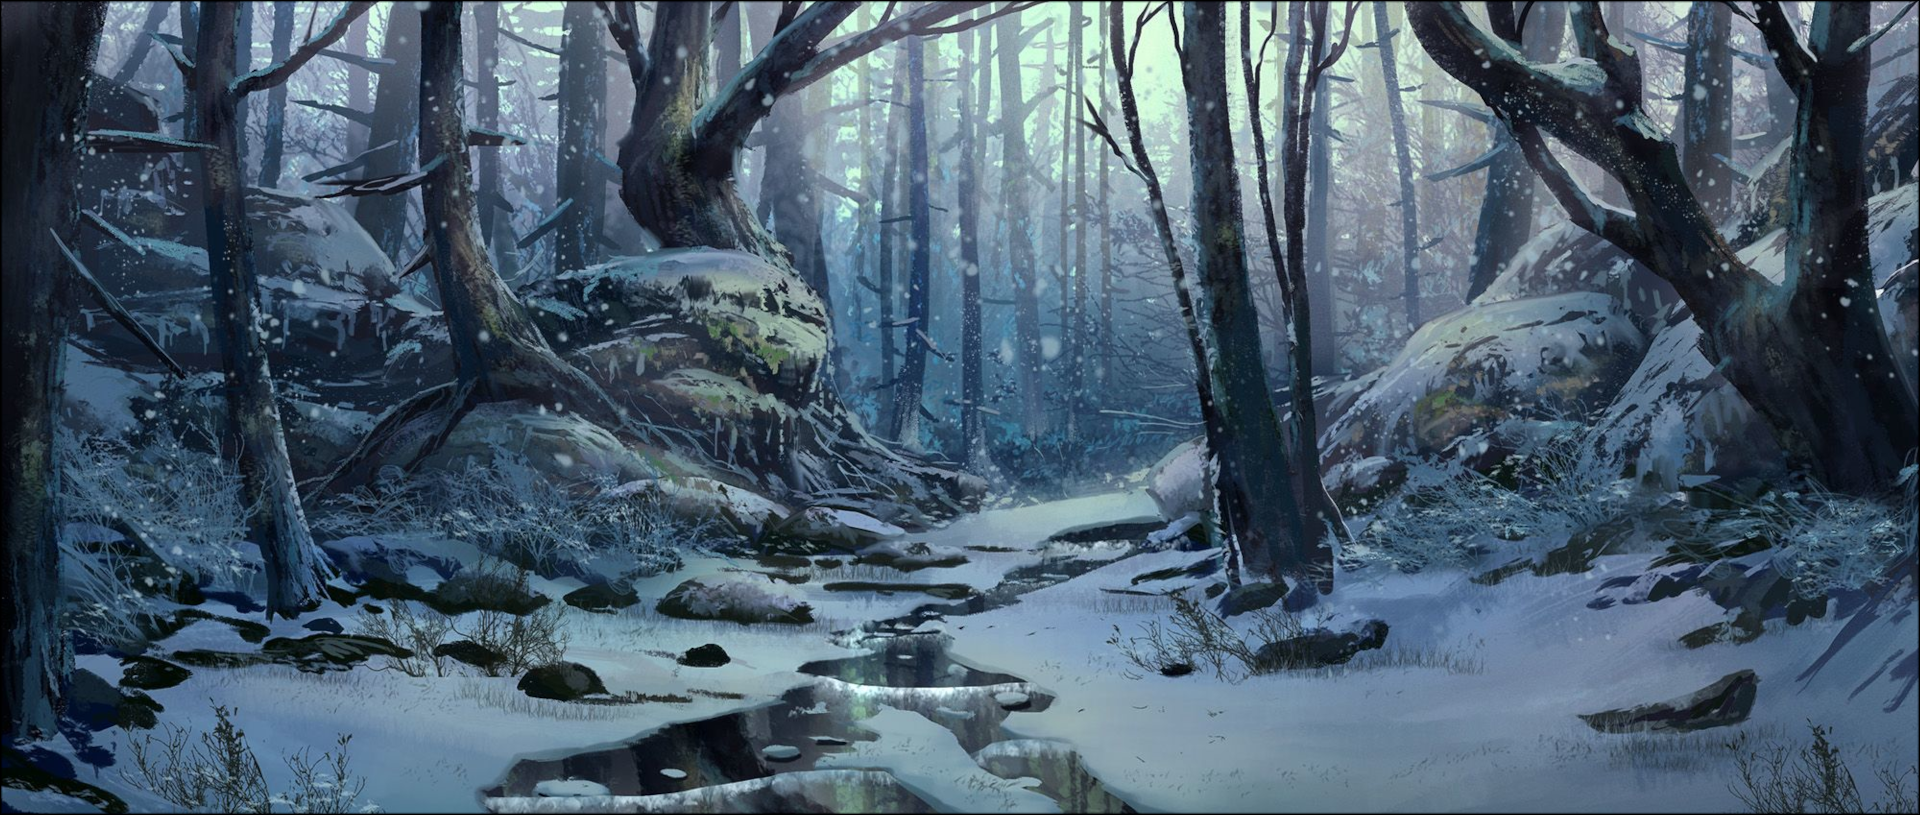
\includegraphics[width=0.95\textwidth]{01yuadrem/img/11tallwoods.png} \
        \centering \large{\textbf{The Tallwoods}}
    \end{DndTable}
\end{table*}

\subsection*{Northern Territories} \label{ssec::northernterritories}
The northmost region of Yuadrem, the Northern Territories are comprised by the Whitenorth, the Red Islands, the Tallwoods, the Blank Fields, and the Sulfur Lake.
The region is split by the Wall of Ice and Stone, a colossal mountain range that spans from coast to coast.

North of the wall is Whitenorth, an area split between the ancient ird kingdom of Krudzal and the territorial giants of Jatuunsa.
Its few inhabitants are beings of extreme resilience and fierceness, acclimated to the harsh habitat.
First among these are the giants, mountain-sized creature of stone, ever locked in war with Krudzal.

The middle of the region is characterized by the endless mists.
The area coincides with the north pole, and is inexplicably warm and misty despite its location.

To the west of Whitenorth is the Red Fjord, named so by its most common tree, the red maple.
The are is regarded sacred by the Krudzalians, who believe it to be the resting place of the sun god, Jua\~nanisz.
The fjord is currently occupied by Ribinhep, a uman nation ever standing up against the northerner irds.

Below the Wall of Ice and Stone are the Tallwoods and the Blank Fields.
The Tallwoods are an association of pine and redwood forest, using the mountains to hide from the cold winds.
The forests are devoid of civilized life, and the stone trolls who inhabit them make sure that they stay that way.

The Blank Fields are a vast, freezing tundra.
The low temperatures and strong winds in the area prohibit the growth of any vegetation.

The west of the fields are known as the Wurmlands, and they are solely inhabited by wurms.
Wurms are large reptile-like creatures that attack all foolish enough to approach their subterranean colonies.
The eastern portion of the land is filled to the brim with a variety of bughna gat tribes, ever in conflict for the large reserves of copper and coal in the mountains.

East to the fields is the Arctic Archipelago.
This cluster of islands separate the Whaler's Sea from the frigid ocean up north.
Mostly bare and desolate, the islets equally house ird, gat, uman, and zaloth settlements.

The strongest force in the archipelago is the Kaldrathal nation.
Having the only vessels strong enough to withstand the ship-sinking idzels, they regulate commerce in the entire archipelago.
% idzels or idzelal are inspired on Illhevi (https://abookofcreatures.com/category/iceland/page/2/).

% !TEX root = ../main.tex

% \begin{table*}[b]%
%     \begin{DndTable}[width=\linewidth]{X}
%         \centering
%         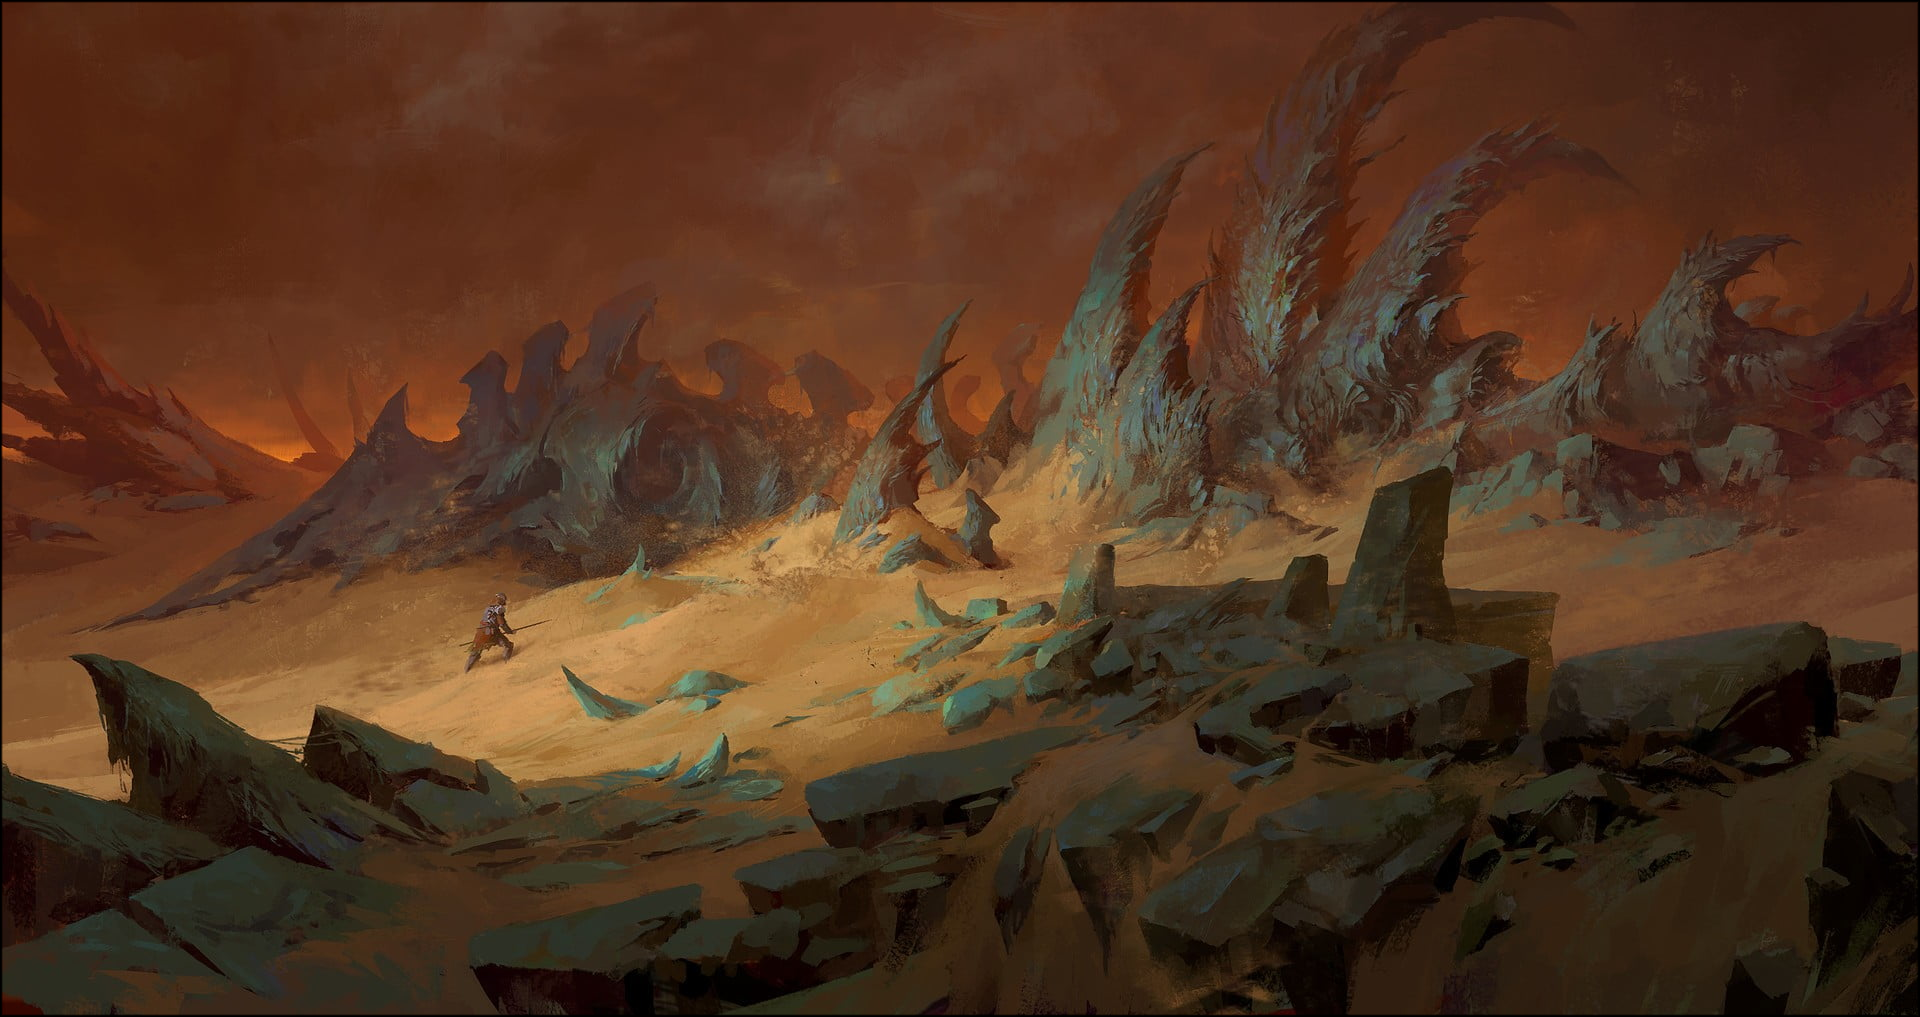
\includegraphics[width=0.95\textwidth]{01yuadrem/img/12dead_sea.png} \
%         \centering \large{\textbf{The Bone Cliffs of the Dead Sea}}
%     \end{DndTable}
% \end{table*}

\subsection*{The Three Deserts} \label{ssec::threedeserts}
Effectively splitting Yuadrem in half are the three deserts: Zoedrem, Zashlath, and the Dead Sea.

Zoedrem is a large expanse of yellow sands the embraces the waves of both the Whaler's Sea and the Teal Ocean.
The desert runs undisturbed from the Sulfur Lake down to the Defiled River.
It is commonly regarded as the most forgiving of the three deserts.

More fearsome than the sands are its inhabitants, the five dratl ird houses of Zoedrem.
Descendants of the fallen empire of Hulnar, they hide their settlements along the stone cliffs.
They are constantly in search of prey, robbing and murdering any traveler foolish enough to travel in their territories.

At the easternmost point of Zoedrem is the Sylvan Canyon, the only area in the desert able to host life.
The gorge is the home of the independent nation of Viphoger.
Apart from its inhabitants, the canyon's soil has rich natural deposits of oil, salt, and gemstones.
These resources grant Viphoger a strong economy despite its young age.

Southeast of Zoedrem and across the Ichor Mountains lie the Dead Sea, an artificial desert created by the tall kin's folly.
The desert's sands are of a sickly gray color, and any creature that inhabit the land for too long suffer particular mutations.
Its inhabitants, the treb gats and the cursed umans are perhaps the best examples of this.

The sands become blacker the more you approach the spire, the largest mountain in Yuadrem.
The et city of Jan'krug stands atop it, where the ritual that caused the Schism took place.
A long chasm divides the eastern region of the Dead Sea, remnants of the passage of the breathing island, Cabb Goem-Rlamesh.
Surrounded by hill, mountain, and river, the desert naturally prohibits passage to it, almost as if it's protecting a twisted secret.

Apart from the kins that call this desert home, the Dead Sea is infested with other monstrosities.
These are categorized into two: The Nyxborn and the children of Cabb.
The former are giant insect-like creatures that can be as large as an elephant and as precise as a mosquito.
The latter are tormented amalgamates that dislodged from Cabb Goem-Rlamesh, ever haunted by insatiable hunger and unending pain.

% Along with the tortles, grungs, and umans, the Schism brought forth terrible creatures known as the Nyxborn.
% These insect-like monstrosities can be as huge as the Mirmekolon, a colossal ant-lion hybrid, or as precise as the Khanokoladtes, a palm-sized moth that pierces skulls with its sharp dart-like mouth.

South, through the Hammerfall canyon, is the Zashlath desert, the driest of the three.
Featureless and white, only the hardy sunstruck oths have been able to call the desert home, and even they are wise enough to only establish by the neighboring mountains.

Zashlath practically receives no precipitation, and its white-colored sands reflect the scorching sunlight to deadly effect.
Truth is the desert remains largely unexplored to this date, and only rumors exist about the horrors that might hide among its sands.
Famous among these is the Haimorrois, a red horned snake whose bite forces the blood out of one's body.

% !TEX root = ../main.tex

\begin{figure}[t]
    \centering
    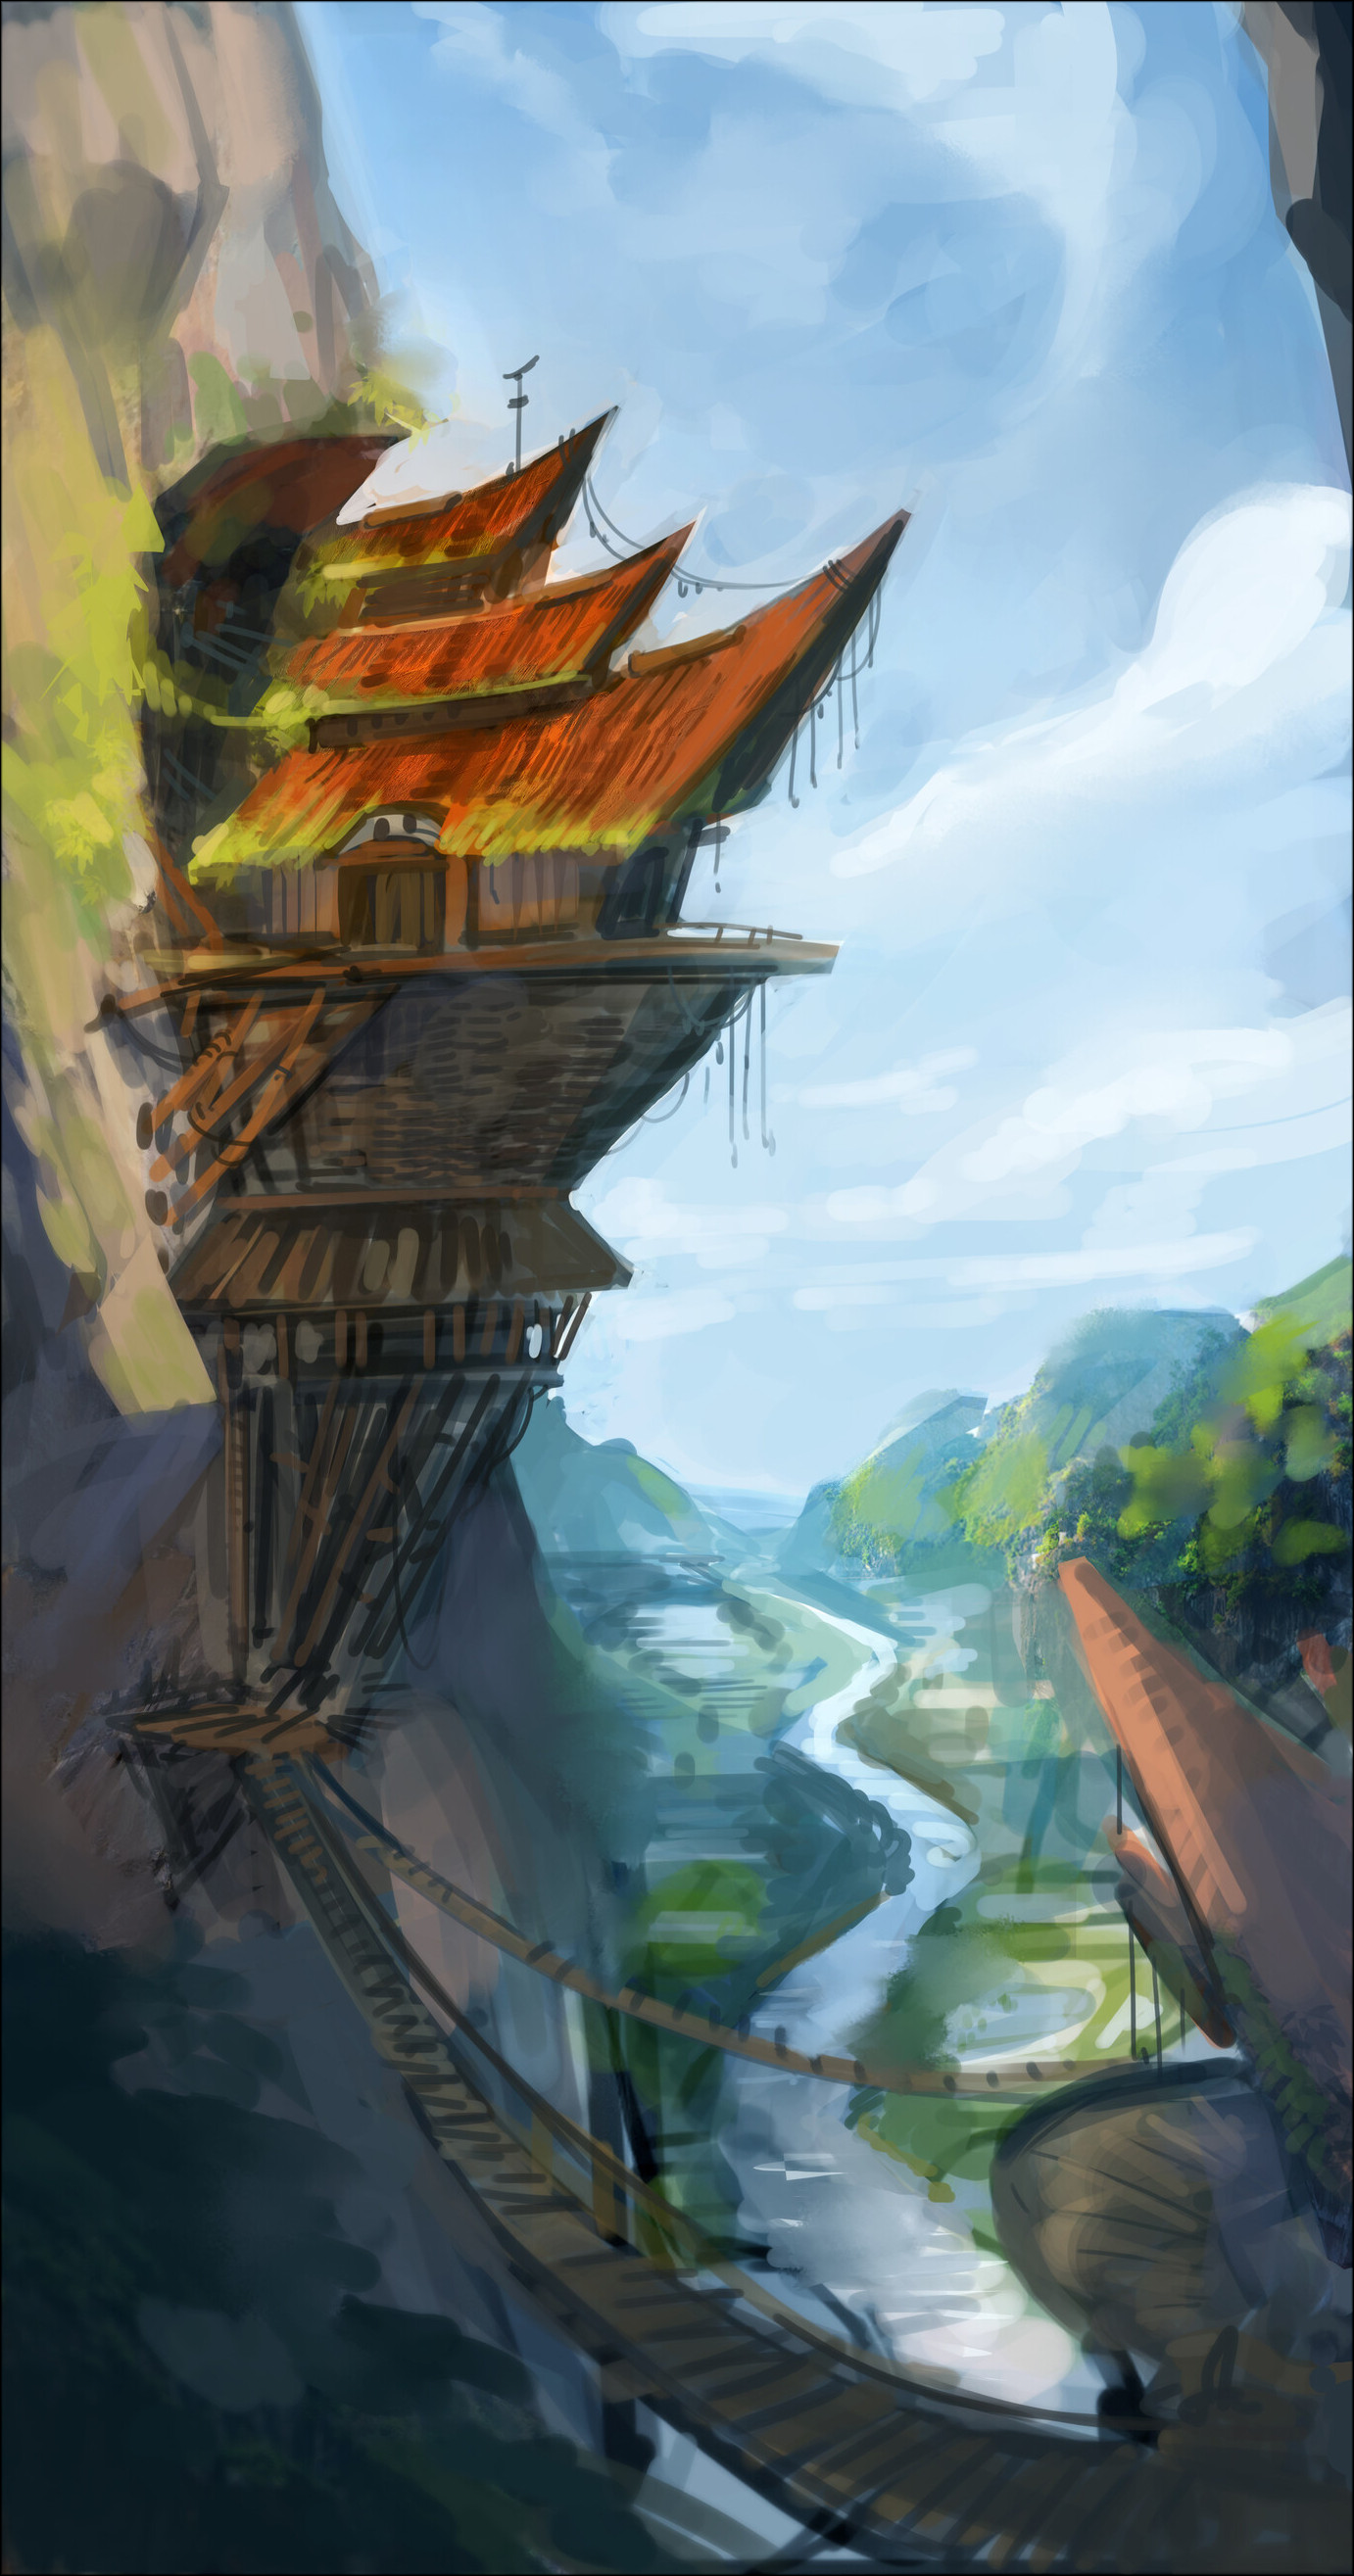
\includegraphics[width=0.46\textwidth]{01yuadrem/img/13siszgoel.png}
    \caption*{\centering \large{\textbf{Siszgoel, Kaldrathal's Capital}}} % TODO: Check if I can change the font of the caption
\end{figure}

\subsection*{Whaler's Sea} \label{ssec::whalerssea}

% intro
The cradle of modern civilization, the Whaler's Sea is home to both well-established and blooming countries.
Its coasts protected from harsh winds by mountain ranges and its cold waters supplied with both whale and idzel, the region couldn't be a better location to develop the modern world.
Idzels are large whale-like creatures known for their ship-sinking fury and their large supply of the valuable ambergris, the main ingredient in artificial qualars.

% Krejek and Kaljek
Sitting at the middle of the sea are the two southernmost islands of the Arctic Archipelago, Krejek and Kaljek.
The first is a large island covered by mountains, rocks plains, and deciduous forests.
It serves as the mainland for the independent nation of Kaldrathal.
%, who competes with Sulia as the main exporter of nitrate.

Starting out as a Krudzalian colony, they merged the quench-hardened steel of the thulkraka irds with their natural supply of nitrate.
This combination produces resilient steel firearms, including cannons, muskets, and flintlock handguns.
They remain the only exporter of these valuable weapons.

Kaljek, the smaller of the two islands, is a desolate land, with only few pine and birch forests.
It is separated by four nations inhabited by gat and ird alike.
While historically peaceful towards each other, they have recently been divided by conflict, all over the recently discovered gold veins that hide under their land.
% 661 AS: gold veins found under the ground.

% southern coast
South of both islands are the Horned Shores and the Fesh Peninsula.
The first is known for its calm, dry mediterranean climate, its sparse forests, and the great concrete gat city-states that rise from its ground.
Most of the land is devoid of natural resources, with scarce mines and low-quality wood.

% eastern coasts
East to these lands is the Fesh peninsula, an area inhabited mainly by gats, tortles and thulkraka irds.
A humid subtropical climate permeates the cape, and it is known for its harsh, capricious waters and frequent storms.
Also well-known are the tortles inhabiting the small island of Mbeat, for it is the only place where they have met safety after their arrival in Yuadrem.

In both regions lie the oldest nations of Yuadrem, the Seven kingdoms of the Sea.
Historically renowned raiders and pillagers, they are now famous for their passivity --- focusing on enterprise and artisanship.
What they offer is their expert craftgatship, and among them are the only bonecarvers capable of manufacturing qualars.

% western coast
Finally, to the west of Krejek one can find the two daughters of Palegna, the countries of Sulia and Drer.
The two nations were in a sense ``commisioned'' by the oth nation of Palegna.
Sulia was born to control the worrying growth of the Sulfur Lake, and Drer to restrict the growth of the bughna gat tribes of the Blank Fields.
% Both countries also served as an experiment of sorts for the word-obsessed oths, since the official language in both nations is the artificial Standard Language created by them.

Sulia benefited greatly from what would originally be their burden, and have developed a refined industry based on sulfur.
Their sulfur-based fertilizer is the basis of modern agriculture, their fiery blackpowder is only matched by Kaldrathal's, and their self-preserving wines are a taste craved all around the continent.
% They also have great sulfur-inlaid furniture!

Drer, in stark contrast with its sister, is a nation whose economy solely depends on pillage.
Re-imagining Sulia's blackpowder, they use their fire-bearing weapons to push back and raid their northern neighbors.

% !TEX root = ../main.tex
\subsection*{Beryl Sea} \label{ssec::berylsea}

The Beryl Sea is a searing, tropical region, ever battered by violent winds and waters.
The region is tapered in rainforests, and it houses two of the largest nations in Yuadrem: the warring Jenkashian empire and the mysterious Gannag.
The coasts see few other countries, and seldom do ships sail in these lands.
% Apart from the two, the coasts are also inhabited by a somewhat limited variety of countries, including the ancient Edede, the resilient Voskferm, and the strange Na'ane.

% Drejeck
Westernmost of Yuadrem is the thick, dark, and moist jungle of Drejeck.
Drejeck is the birthplace of the savage naenks and the ceremonial tsaneks, and is now entirely occupied by their nation, Gannag.
Despite being born even before the Schism, the beings of Gannag are primitive and untamed, and keep their tribal ways despite regular contact with more sophisticated cultures.
The jungle is also inhabited by large and dangerous beasts that threaten the unprepared explorer, like the aggressive nadubis or the silent whowie.
% And the bulettes and the Yara-ma-yha-who.

% Fog Gorge
East to Drejeck is the Fog Gorge, a well-forested canyon island ever enveloped in fog.
While primitive, the tribes of Gannag are far from free-living, and are bound by strong shackles to their superiors.
While naenks are used to this hierarchical system, many of the more intelligent tsaneks grow tired of it over time.
A hundred and fifty years ago, a group of tsaneks went as far as to establish their own independent tribe of Na'ane in the misty island, abandoning their brethren in favor of an unrestrained lifestyle.
Freely they carry on with their ceremonies and rituals, protected from their neighbors by mist and stone.

% Qul archipelago
Further east one finds the Qul archipelago, a clump of islands that collectively served as the birth bed of the Jenkashian empire.
Jenkash is a coalition of tribes that only managed to unite after cutting down the last tree in their mountainous islands.
This led to an explosive expansion of their empire, and they swiftly conquered the neighboring lands.
Their territories now span most of the coasts of the Beryl Sea.

The archipelago itself is absolutely desolate, with barely any tree or foliage growing atop its igneous rock.
Perhaps the only bright side of this uncontrolled deforestation is the fact that it brought to light the iron and diamond veins in the eastern side of the archipelago.
These resources are heavily exploited by the qulbaba irds, and led to their signature diamond daggers.

% Dratl'fal savanna
North of the archipelago is the Dratl'fal savanna, occupied entirely by Jenkash.
The only plant that freely grows in the savanna is bafarmat, a purple moss covering its entire southeastern coast.
This plant is the primary food source of the cavernous species that live under the ichor mountains.
Its spread has allowed the hornbeetles to move into the area, a strong species of giant blue beetles that served as companions to the now ruined nation of Phrisht.

In oldentimes, the dry lands served as the birth bed for many gat city-states, of which only Dzorvepem and Jorea remain standing, now part of Jenkash.
Despite its lack of resources, the whole area was sought after by the now divided empire of Hulnar, who battled against the blooming nation of Phrisht for more than 300 years for it.
This everlasting conflict was only stopped by Jenkash, who in their thirst for conquest ended up dissolving the untiring countries.

% \begin{figure}[t]
%     \centering
%     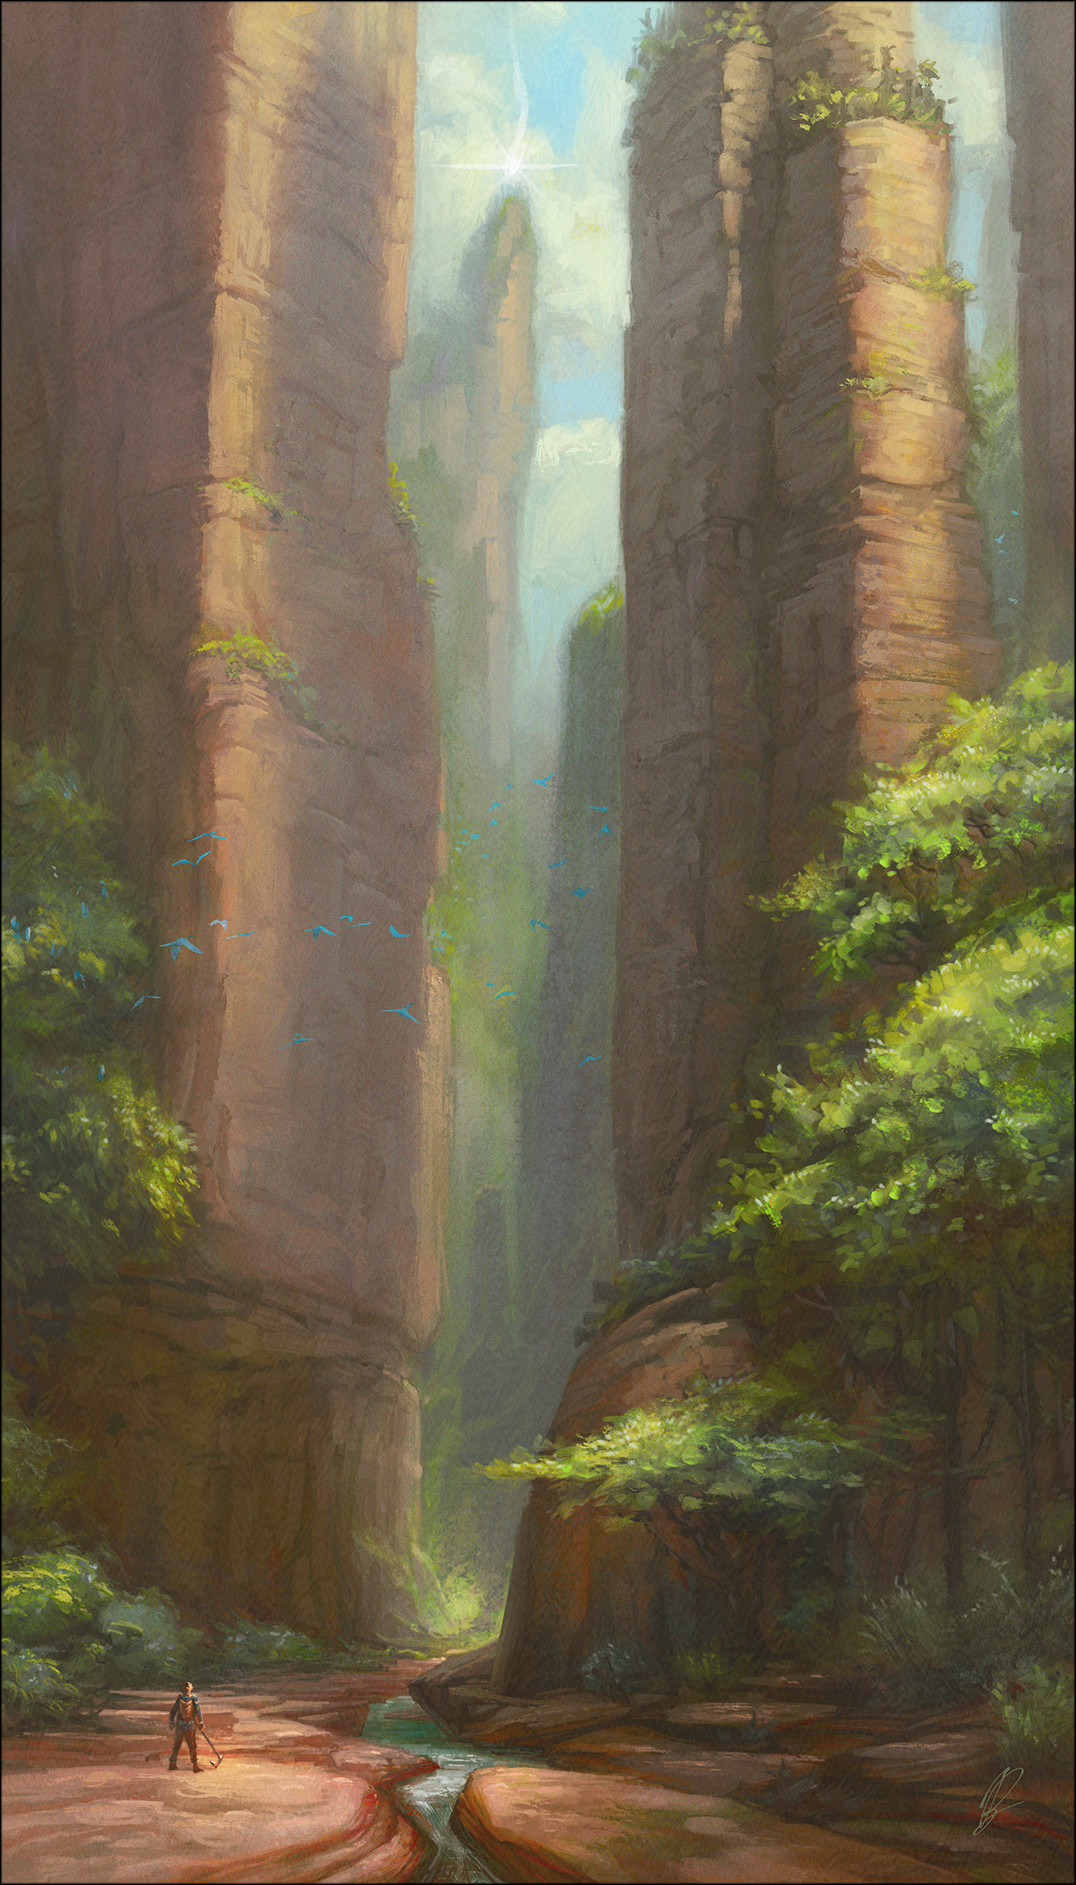
\includegraphics[width=0.46\textwidth]{01yuadrem/img/14fog_gorge.png}
%     \caption*{\centering \large{\textbf{The Fog Gorge}}}
% \end{figure}

% Ironlakes Island & Zashlath savanna
Moving to the easternmost portion of the sea one can find the Ironlakes Island and the Zashlath savanna.
The former is a large island full of forests and lakes.
It was historically a part of the peaceful marset nation of Edede, but most of it now belongs to the warring empire.
The Zashlath savanna is the area west of the desert, protected from its dry air by the moisture of the cerulean waters.

% !TEX root = ../main.tex

\begin{table*}[b]%
    \begin{DndTable}[width=\linewidth]{X}
        \centering
        \includegraphics[width=0.98\textwidth]{01yuadrem/img/15om.png} \
        \centering \large{\textbf{Om, Isken's Capital}}
    \end{DndTable}
\end{table*}

\subsection*{Barbaric Territories} \label{ssec::barbaricterritories}

To the east of Yuadrem are the Barbaric Territories, a region defined by the brutality of war and the greed of an empire.
From north to south, the land can be divided into five areas, each with its own distinct characteristics: the Drylands, Cabb Goem-Rlamesh, the Shield Sea, the Chirping Wilds, and the Xuam Peninsula.

% Drylands
Northernmost are the Drylands, a field devoid of trees or any sort of tall flora.
The area is plain and parched, dried over the years for its lack of rains or rivers.
The northernmost area of the savanna remains bare to date, and is the most tortuous stretch between the Fesh Peninsula and the southern nations.

% Mzavit river and southern savanna
Down across the Mzavit River, the savanna becomes humid and with this water comes civilization.
A wide array of gat city-states have been established here.
Able to withstand the thunderous force of the Jenkashian and Iskenese armies and the hulking chimeras from the Next, these states are noteworthy for their fortitude.
Of special note is the adamant country of Byurev, who have halted the growth of Isken for almost three centuries.

% Cabb Goem-Rlamesh
% NOTE: In the whole island of Cabb Goem-Rlamesh a faint crying sound can be heard.
Off the coast of the Drylands lies a place known as the breathing island, Cabb Goem-Rlamesh.
A harrowing immensity, the landmass is constructed entirely of flesh and bone, and is believed to be what remains of the ets.
Not much is known about the island, and none of the few explorers who have travelled to it retain their sanity.
The mad tell tales of a mortifying city of flesh, and of strange, shape-shifting inhabitants.

% Shield Sea & The Nest
% Wrong information - geomancy was invented by an ancient civilization that warred with the tall kin eons ago, but was erased from history by the victors. There are ruins from this civilization at the basin of the lake, and Fo is the last remaining member from it.
Southwest of the Drylands rest the Shield Sea, an enormous body of water fed by a wide array of tributaries from the Forking Peaks.
In antiquity, the ruined ird civilization of Hairuus invented the art of geomancy in its coasts, raising from the basin the island of ``The Nest'' at its center.
The island currently hosts only one being, Fo.
Fo is a strange creature, rumored to be out of this world.
It welcomes visitors with a variety of fierce chimeras.

% Chirping Wilds
Southeast from the Drylands and passing through the Do Nana swamp are the Chirping Wilds, a vast and largely untamed rainforest.
The jungle is inhabited only by the Iskenese empire, a large grung nation that expelled the original ird and marset population.
The only territories currently not held by the grungs' military might are the strong qulbaba irds of Harual to the west, and the marsets of Uzuz from the Xuam peninsula.

The Xuam Peninsula is the southermost point of the Barbaric Territories, and is located just south of the Grasping Gulf.
The region has facilitated the development of Uzuz due to the heavy presence of wurmroot, a white-leaf poplar tree that is conveniently toxic to all foreigner kins, specially to grungs.

% !TEX root = ../main.tex

% \begin{table*}[t]%
%     \begin{DndTable}[width=\linewidth]{X}
%         \centering
%         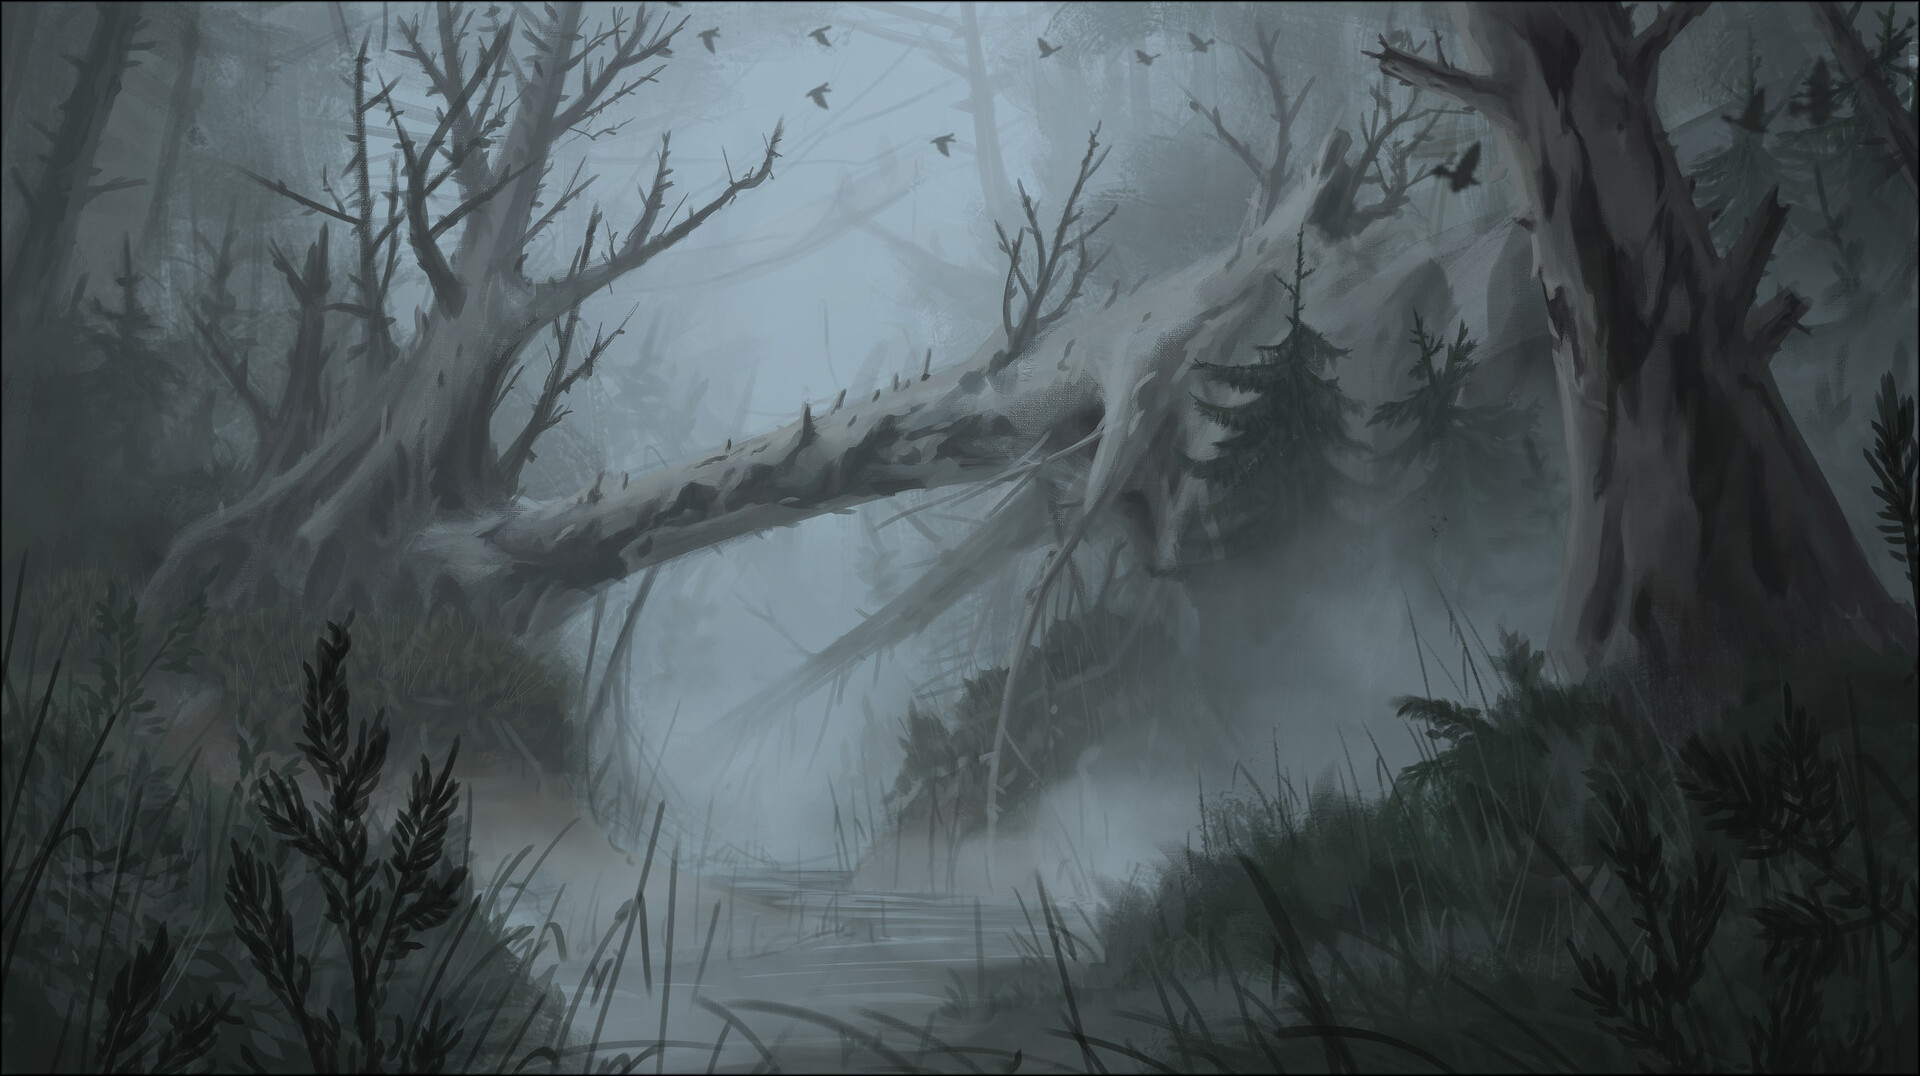
\includegraphics[width=0.98\textwidth]{01yuadrem/img/16pale_blemish.png} \
%         \centering \large{\textbf{Forests Surrounding the Pale Blemish}}
%     \end{DndTable}
% \end{table*}

\subsection*{Wildlands} \label{ssec::wildlands}

% intro
The southernmost region of Yuadrem is aptly named the Wildlands, for it is a large expanse of untamed fields, forests, and lakes.
Starting at the bottom-most part of the forking peaks, the area has seen very little intervention from the civilized world.
This is attributed to the fact that the Wildlands are infested with both deadly creatures and strange tide-altering illnesses.

% Savage Plains
Just below the forking peaks and the Beal river is the northmost point of the Wildlands, the Savage Plains.
They are a humid subtropical area covered by marshes and plains, with few patches of forest in-between.
Fed by many rivers from the mountains, the lands define the southern territories of the Iskenese empire, expanding thorough the whole region.

However, Isken's grip on the Savage Plains is tenuous at best, as the region is as much controlled by the grungs as it is by the local wildlife.
Just as in the forest below, a great variety of foul beasts and creatures can be found in these swamps.
Of special note among these are the giant mole-like jinshus, beasts unique to region who suffocate the unprepared by sinking them beneath the earth.

% Everwoods
As dangerous as these plains are the Everwoods, the forest that grows south of them.
This ancient woodland used to be a place of respite after the harsh swamps, but all that swiftly changed about 400 years ago.
In an attempt to manipulate the tides, the Rashiist school of thought from Ignelli summoned The Sorrow into Yuadrem.
The Sorrow is an entity of unknown origin, who seeped into Yuadrem due to the Rashiists folly.
On arrival, it swiftly slayed all members of the school of thought, and brought fourth with it strange creatures and diseases that now plague the once peaceful forest.
This event came to be known as the Tidal Sway.

% Pale Blemish
Not only bringing forth pain and disease, the Tidal Sway also ravaged the land around Ignelli, area now known as the pale blemish.
All flora was destroyed, and the ground turned into badlands.
The field now serves as a grim reminder to all of the dangers of manipulating the tides.

Despite the destruction, the scholars from the Igneist school continue to work in their temple, studying the tides and The Sorrow.
Perhaps one day they'll achieve their goal and undo their sister school's sins, expelling the Sorrow and healing their lands.

% Niknek Peninsula
West of the Everwoods is the Niknek peninsula, a thin, elongated stretch of land filled with volcanoes and gorges.
The cape was spared from most of the effects of the Tidal Sway.
Niknek and the nearby Vuvu Isles now house the refuge marsets from the Ironlakes Island.

% Elderberry Wilds
At the southern tip of Yuadrem are the Elderberry Wilds and the Ironwoods, a set of pine and spruce forest surrounding the Manta Sea.
The area is partly occupied by Gronselar, an old and forgotten colony of Krudzal.
% Not much is known about these forests due to their remote location.
% Not much is known about the area due to its remote location, but even here a semblance of civilization exists. in the form of the ird nation of Gronselar, and the regions of Froibias, Glameas, and Visilias.


% !TEX root = ../main.tex
\section{Cultures} \label{sec::cultures}

\DndDropCapLine{U}{pon their abandonment, the kins were}
quick to travel to the far reaches of Yuadrem, carrying civilization with them.
Over the years, languages, religions, and rites of different natures spreaded far and wide to create the complex network of cultures we see today.

% !TEX root = ../main.tex
\subsection*{Religions} \label{ssec::religions}

\DndDropCapLine{R}{eligion is an important part of life}
of the many cultures of Yuadrem.
Some worship specific pantheons of gods, others praise unpersonified concepts, and a selected few worship nature itself.
% In the times before the schism there was a wide belief that the tall kin could answer prayers, but their worship is now forbidden in most of the continent.

% The true existence of these divinities is a widely discussed subject, but their worship is undeniable.
From the nature-worshiping folk of Jenkash to the god-birds of Krudzal, each culture performs a set of rituals in the name of their deities, and some even claim to be able to channel their divine power.
While it might be hard to pinpoint the exact number of religions in Yuadrem, a few are built into the fabric of civilizations, and are easy to tell apart.

\subsubsection{Igneism}
The oth scholars hailing from Ignelli were the first to conceptualize the tides.
They learned that the tides are intrinsically woven into sentience.
As tightly tied threads between sentient creatures, a change in the tidal alignment in one has profound effects in that of those nearby.
% Each tide was then assosiated with a symbol and an entity, to give a more concrete face to it and facilitate its worship.

The blue tide is represented by a blue unfinished book, representing the eternal pursuit of knowledge.
The gold tide is symbolized as a seed or an egg, telling of the coming of future life with proper nourishment.
Indicated by a torch, the indigo tide tells of the truth revealed under light, and the punishment exerted upon those who hide it.
A broken compass represents the red tide, representing the roaming of those who walk without roads.
The silver tide's symbol is a bell, denoting the attention obtained by those who seek fame.

Nearing the year 174 AS, the knowledge of the tides split the Ignelli school in two - The Igneists and the Rashiists.
% The Zelseists, who simply sought to further understand this new discovery, and the Rashiists, who attempted to wield and manipulate them.
The latter created a system of magic known as Rashid, with which they could potentiate the tidal alignment of others.
Despite the warnings issued by their sister school, the Rashiists honed their craft to its maximal potency, and suffered severely from it.
Their actions awoke a strange an antique and mysterious creature: The Sorrow.

% The Sorrow is a being of indescribable shape who was summoned to Yuadrem by the Rashiists' folly.
Breaking the mind of any who lay their eyes upon it, it swiftly took the lives of all who corrupted the balance of the tides, thus ending the Rashiist school's folly.
Its presence caused the pale blemish, and with it came horrid creatures known now as the xuagra.
Seeing the destruction caused by their sister school, the Igenists hid the knowledge of their former brethren, forbidding Rashid in any shape or form.
% Finally, they changed their own name to Igneists in an attempt to bury the other school in anonymity.

Igneism is the worship of the tides as a concept, and the active pursuit of keeping the five balanced.
Igneists recognize that sentience cannot exist without the tides, and praise them as thanks for the capacity of independent thought.

\subsubsection{Tanethism}
Across the long history of the Seven Kingdoms, varied deities were gradually associated with many different concepts, and any gat would pray to different gods at different times and circumstances.
For example, one might say a prayer to the Traveler for luck, make an offering to Tamaz before going to the market, and pray to appease Matevos when a severe storm blows in --- all in the same day.

Independent to any institution, the gat scholar Taneth officially published ``The Rituals and Gods of the Gats'' in 511 AS.
The book was an exhaustive compilation of the more than a thousand deities that were praised by the different kins of the Seven Kingdoms, and proposed a reduced pantheon of 15, distilling the chaotic pantheon into the main gods.
Taneth's work was barely known during their life, and they died without due recognition.

Later, in the year 577 AS, the king of Khedrat Olag the Immortal sought a method to reduce the religious disparity among their people.
Either by divine will or happenstance, they came upon this book by Taneth, and established Tanethism as the official religion of Khedrat, imitating the well-established creed of other nations.
By command of the government, many churches were erected in the name of each god, and the many gods of the gats coalesced into a more sober pantheon of 15.

Many have a favorite among the gods, one whose ideals and teaching they make their own.
A few even dedicate entirely to a single deity, serving as a priest, acolyte, or champion of that god's image.
Famous among these devout beings are the nimrod, an organization of zealous hunters of Phusinhe who pursue all who disturb the balance of Yuadrem.
Well-known as well are the followers of Havetish, a group of gats in golden robes whose goal is to distribute wealth and food to the impoverished hamlets of the inner regions of the Seven Kingdoms.

\begin{table*}[b]%
    \begin{DndTable}[width=\linewidth, header=The Gods of Yuadrem]{p{2cm}p{0.8cm}p{3cm}p{1.8cm}X}
        \textbf{Name} & \textbf{Tides} & \textbf{Domains} & \textbf{Religion} & \textbf{Symbol} \\
        The Scholar  & B  & Reason, Knowledge     & Igneism   & A many-armed blue oth reading multiple books. \\
        The Zealous  & R  & Passion, Zeal         & Igneism   & A red dratl ird standing over a sand dune. \\
        The Star     & S  & Admiration, Fame      & Igneism   & A naked tall one, sometimes replaced by a shadow or a uman. \\
        The Equalist & I  & Justice, Equity       & Igneism   & An indigo gat holding a spear and a coin. \\
        The Altruist & G  & Empathy, Compassion   & Igneism   & A furtive golden marset carrying a basket full of eggs. \\
        The Sorrow   & -  & Balance, Punishment   & Igneism   & An indistinct cloaked figure holding a bloody heart. \\
        Changing God & -  & Secrecy, Manipulation & Rashiism  & A robed oth with a featureless bronze mask. \\
        Febrid       & B  & Intellect, Wood       & Tanethism & A gat forming a crescent moon with its horns. \\
        The Traveler & BR & Luck, Beer            & Tanethism & An indistinct figure cloaked in light brown robes. \\
        Vugar        & BG & Family, Fertility     & Tanethism & A gat prince dressed in a simple silver toga. \\
        Vahagn       & R  & Mountains, Fire       & Tanethism & A red quies holding a colossal mace. \\
        Genadi       & RI & Bravery, Love         & Tanethism & A grung warrior carrying a sword and a lute. \\
        Sakris       & RS & Fun, Wine             & Tanethism & A uman servant carrying cups and wine. \\
        Matevos      & S  & Glory, Water          & Tanethism & An ice zaloth holding a bident and a shield. \\
        Hanutsh      & SB & Teaching, Books       & Tanethism & A tsanek dressed in scrolls and paper. \\
        Tamaz        & SG & Wealth, Silver        & Tanethism & A gray ird eternally flying towards the sun. \\
        Phusinhe     & I  & The Stars, Metal      & Tanethism & A giant tortle with the visage of stars in its shell. \\
        Nadzim       & IB & Justice, the Sky      & Tanethism & A purple oth holding an abacus and a spyglass. \\
        Gathoz       & IS & Secrecy, Murder       & Tanethism & A kinless being with shifting body and face. \\
        Bagrat       & G  & Farming, Earth        & Tanethism & A gat farmer with tools made of gold. \\
        Havetish     & GI & Leadership, Tyranny   & Tanethism & A naenk holding a golden and an indigo spear. \\
        Mziva        & GR & Self Sacrifice        & Tanethism & A blonde marset with a flowered back. \\
        Jua\~nansiz  & G  & Day, Sunlight         & Tsalemism & A rainbow-colored heron followed by northern lights. \\
        Dzadsiz      & R  & Night, Darkness       & Tsalemism & A black raven surrounded by never-dispersing mists. \\
        The Observer & -  & Cosmos, the Unknown   & Cosmism   & A titanic three-eyed slug ridden with tentacles and appendages.
    \end{DndTable}
\end{table*}

\subsubsection{Tsalemism}
It is indubitable that astral concepts are commonly associated to divinities, and no religion reflects this as clearly as Tsalemism.
Tsalemism is a belief that originally gained popularity in the coasts of Krudzal, quickly becoming the official religion of the nation and of many thulkraka irds.
Due to its proximity to the north pole, Krudzal experiences long polar days and nights every year, and this irregular schedule naturally led to the personification of night and day.

Day is associated to Jua\~nansiz, a rainbow-colored heron that brings daylight and colors to the entirety of the polar region.
Jua\~nansiz eternally hunts Dzadsiz, a black raven who in turn seeks to tire the heron and finally feast on its exhausted body.
The birds' duel is unending, and the wreckage of their battle is used to explain the chaotic fjords in the Northern Territories.

The boreal lights seen near the pole are Jua\~nansiz's trail.
The mountainous landscape of the Whitenorth are the places where Dzadsiz fell, struck by the heron.
% The endless mists were created by the raven in an attempt to hide from Jua\~nansiz.
These and many other natural phenomena of the Northern Territories are explained by the birds and their eternal duel.

The two birds are not worshiped equally, but their wrath is feared by all.
A sailor may produce a small temple to appease Dzadsiz before sailing, and a cartographer may sing a praise to Jua\~nansiz before taking flight.

\subsubsection{Cosmism}
While the worship of the tall ones is forbidden, their own religious ideas persist in the form of Cosmism.
Cosmism is related to the search of one's place in the larger scheme of things, dubbed the ``cosmos''.
The Observer is the manifestation of the elusive concept of this cosmos, an omnipresent god observing all of Yuadrem at once.

The ideas behind the doctrine were originally conceived by the ets in time immemorial, and cosmists are generally met with disdain and criticism.
Due to this, many acolytes of the religion practice their rituals in the protection of the darkness, and it's very rare to see a church openly dedicated to cosmism.

Cosmism explains some of the strange phenomena of Yuadrem as the whims and thoughts of The Observer.
The tides are the reactions of The Observer to the actions of each being.
Qualars are the medium by which people can commune with The Observer, granting them some of Their wisdom.

% Cosmists fear the cosmos, and carry strange and surreptitious rituals to appease The Observer or gain its favor.

However, what may be shunned in the surface can always find its place underground.
There seems to be a deep connection between the search of oneself in the larger scheme of things and the ego death experienced in the tsanek melds.
Many temples and ritual places exist in the mushroom cities of the cave-dwelling fungal kin, and cosmism is the official religion of the tsanek nation of Na'ane.
% Tsaneks view the cosmos with curiosity, and seek to understanding through observation and hypotheses.

% !TEX root = ../main.tex
\subsection{Languages} \label{ssec::languages}

\begin{table*}[b]%
    \begin{DndTable}[width=\linewidth]{X}
        \centering
        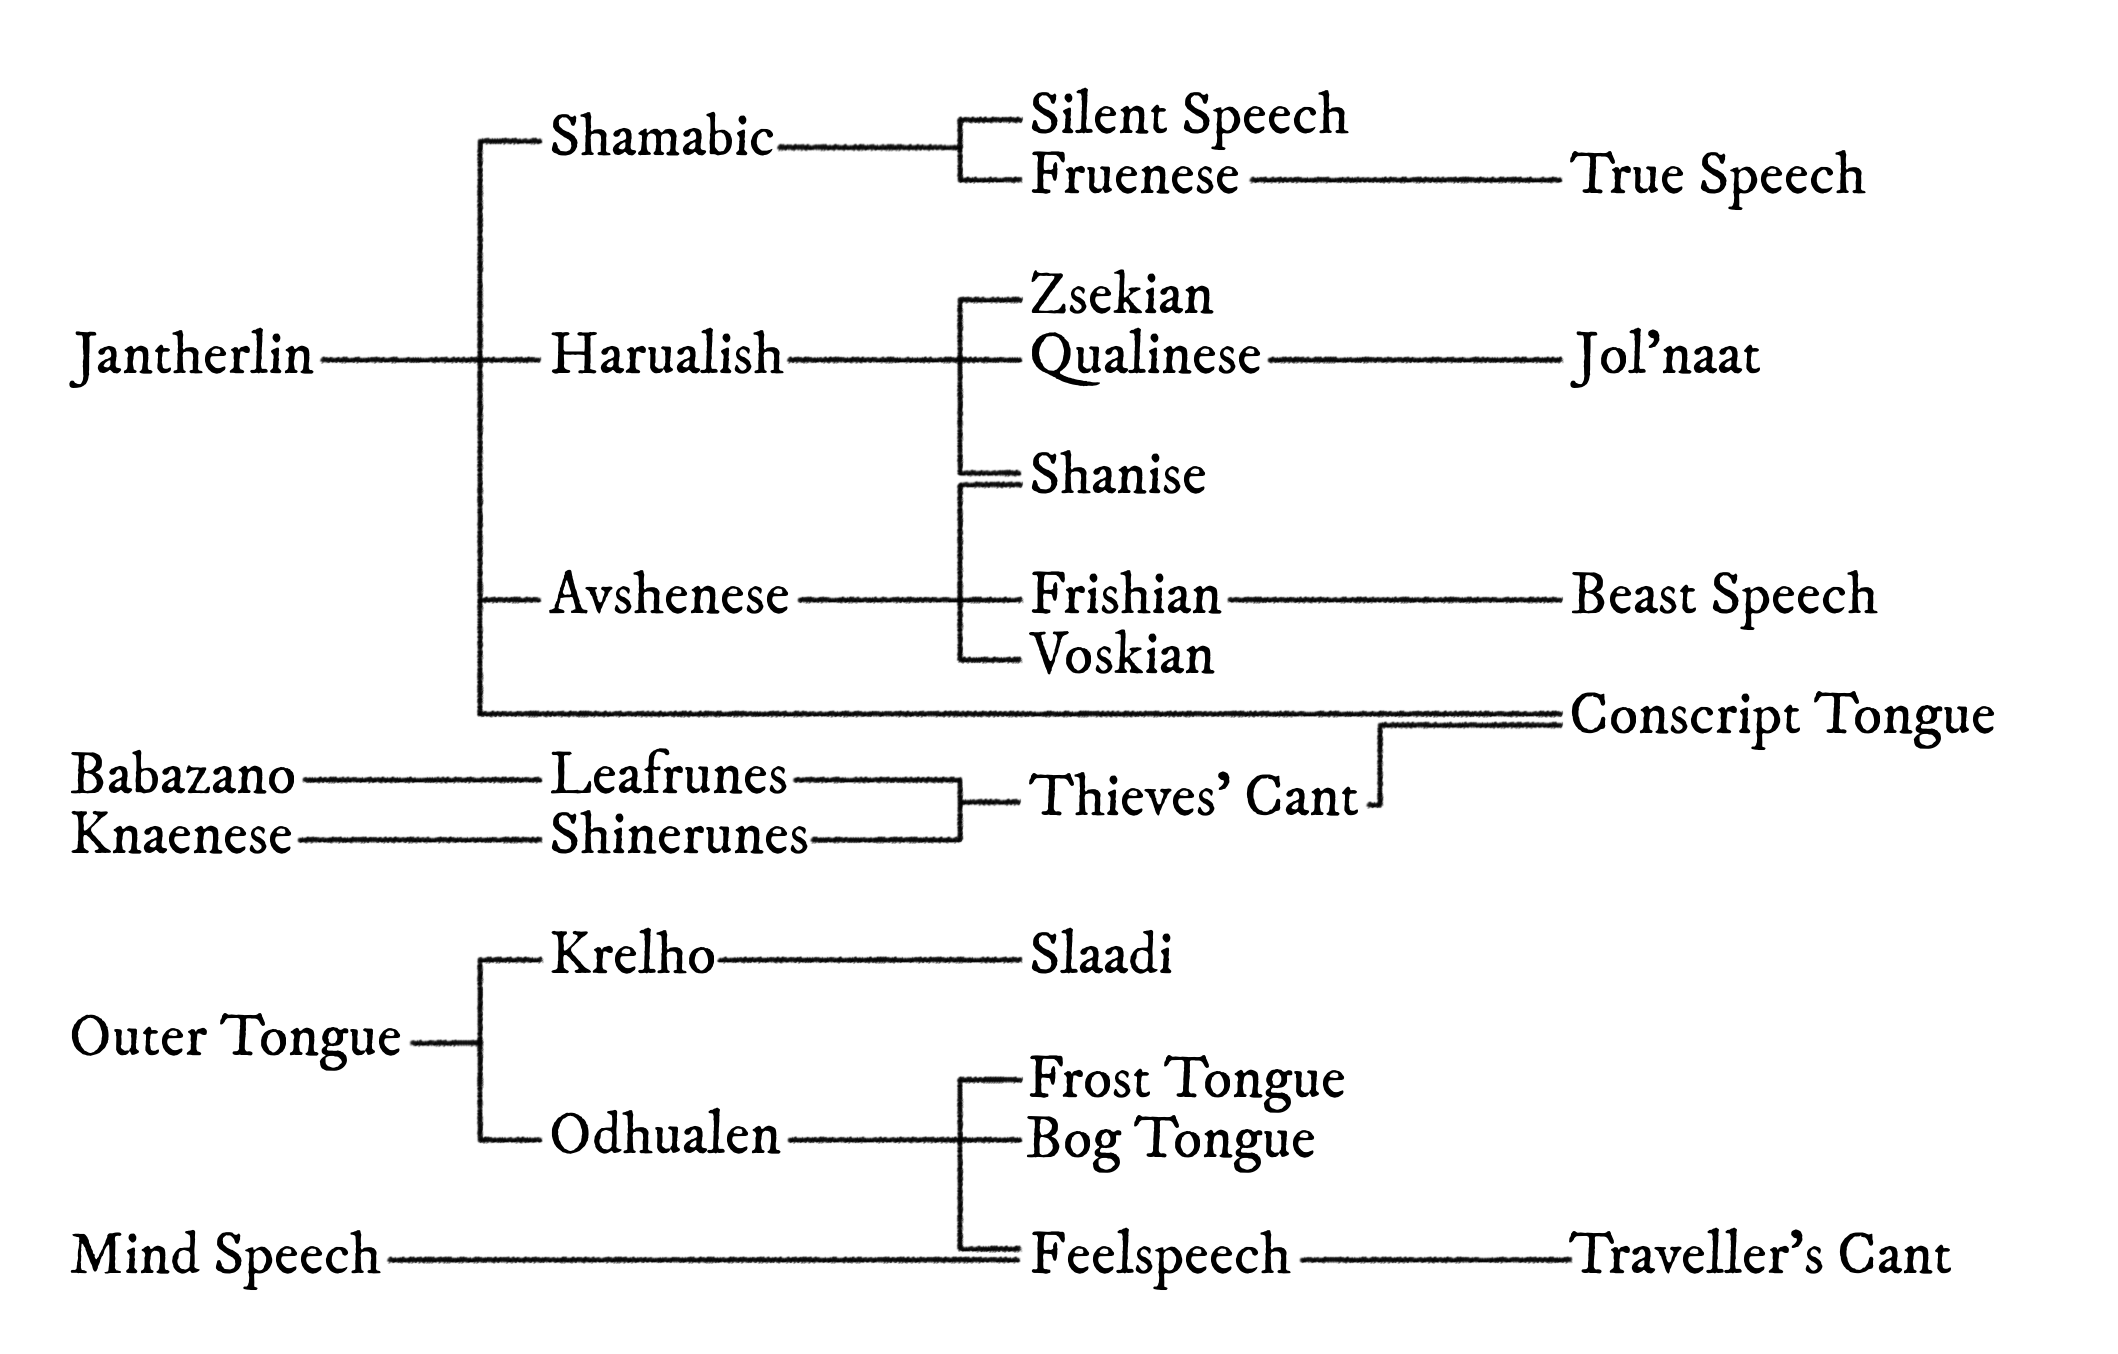
\includegraphics[width=0.99\textwidth]{01yuadrem/img/22languages_map.png}
    \end{DndTable}
\end{table*}

A great variety of languages permeate Yuadrem, both of natural spawn and artificial design.
While it is impossible to identify each tongue and its variations, many efforts have been done over the years to classify the common ones.

Based on lexical and grammatical similarities, languages are separated into four generations, and five distinct families.
The following tables classify these languages, pointing to their script and original speakers.

% As is discussed in the following pages, your country of origin determines your language more than your kin.
% Despite this, some languages are indeed associated to certain kins, as they were the original speakers.

\begin{DndTable}[width=\linewidth, header=First Generation]{p{2.6cm}p{2.6cm}p{2cm}}
    \textbf{Language}  & \textbf{Original Speakers} & \textbf{Script} \\
    Jantherlin         & Ets                        & Varies \\
    Babazano           & Marsets                    & - \\
    Knaenese           & Naenks \& Tsaneks          & Knaenese \\
    Outer Tongue       & -                          & Outer Tongue \\
    Mind Speech        & Zaloths                    & -
\end{DndTable}

\begin{DndTable}[width=\linewidth, header=Second Generation]{p{2.6cm}p{2.6cm}p{2cm}}
    \textbf{Language}  & \textbf{Original Speakers} & \textbf{Script} \\
    Shamabic           & Oths                       & Shamabic \\
    Harualish          & Irds                       & Harualish \\
    Avshenese          & Gats                       & Avshenese \\
    Leafrunes          & Marsets                    & Leafrunes \\
    Shinerunes         & Naenks \& Tsaneks          & Shinerunes \\
    Seedspeech         & Gannagian Tsaneks          & - \\
    Krelho             & Tortles \& Grungs          & Krelho \\
    Odhualen           & Umans                      & Outer Tongue
\end{DndTable}

\begin{DndTable}[width=\linewidth, header=Third Generation]{p{2.6cm}p{3.2cm}p{2.2cm}}
    \textbf{Language}  & \textbf{Original Speakers} & \textbf{Script} \\
    Silent Speech      & Oths                       & - \\
    Fruenese           & Sulian Oths                & Fruenese \\
    Zsekian            & Zsek Irds                  & Harualish \\
    Qualinese          & Jenkashian Irds            & Harualish \\
    Shanise            & Northern Irds \& Gats      & Shanise \\
    Frishian           & Jorea \& Dzorvepem         & Avshenese \\
    Voskian            & Voskferm \& Voskgrit       & Avshenese \\
    Thieves' Cant      & Rogues \& Thieves          & Thieves' Cant \\
    Slaadi             & Slaads                     & Krelho \\
    Feelspeech         & Zaloths \& Umans           & -
\end{DndTable}

\begin{DndTable}[width=\linewidth, header=Fourth Generation]{p{2.6cm}p{3.2cm}p{2.2cm}}
    \textbf{Language}  & \textbf{Original Speakers} & \textbf{Script} \\
    True Speech        & Palegna \& Sulia           & - \\
    Jol'naat           & Jenkash                    & - \\
    Beast Speech       & Jorea                      & - \\
    Conscript Tongue   & Cabb Goem-Rlamesh          & - \\
    Traveller's Cant   & Zaloths \& Umans           & Traveller's Cant
\end{DndTable}

% \subsubsection{First Generation}
% \paragraph{Old Tongue} A very complicated and intricate language spoken by the tall kin, the original settlers of Yuadrem.
% It's spoken form involves various complex articulations and the definition of a word can vary greatly based on the context.
% Additionally, each tall one had their own personal version of the written form, and others would understand it as much as they understood the individual.
% % This makes the reading of the old tongue extremely difficult for the kin that remain in the world, since understanding a particular tall one's scribbles essentially requires understanding their own version of the language.
% % Nowadays, only scholars and archaeologists understand the language, and it is not normally used anywhere.
% \paragraph{Marset Tongue} Every marset is already able to speak this strange, repetitive language.
% The marset tongue only has ten consonants, and ten verbs.
% % The rest of their vocabulary is built up from there, making their language very difficult to speak or understand by kins other than the marsets.
% Marset tongue can be spoken in one of two ways: soundlessly, through lip reading, or screamed as loud as possible, with no middle ground.
% The language cannot be written down.
% \paragraph{Naenk Tongue} Short words and strong consonants define the naenk tongue.
% Lacking lips and teeth, naenks make heavy use of their alveolar ridge and hard palate to produce syllables.
% The written form of the language involves carving lines and holes onto bark or stone.
% \paragraph{Outer Tongue}
% \paragraph{Mind Speech}

% \subsubsection{Second Generation}
% \paragraph{Dust Tongue}
% \paragraph{Ird Tongue}
% \paragraph{Gat Tongue}
% \paragraph{Leafrunes} Very easy to learn, but kept secret by the archer kin.
% A marset will teach this set of runes only to creatures that it deeply trusts, and only if it's strictly necessary.
% Ten leafrunes exist, all of which are used individually and to convey very simple meaning.
% % \textit{colony}, \textit{danger}, \textit{fun place}, \textit{hiding spot}, \textit{observation point}, \textit{predators}, \textit{road}, \textit{sacred place}, \textit{source of food}, and \textit{source of materials}.
% \paragraph{Shinerunes}
% \paragraph{Krelho}
% \paragraph{Nomad Tongue}

% \subsubsection{Third Generation}
% \paragraph{Silent Speech}
% \paragraph{Standard Language}
% \paragraph{Zsek Tongue}
% \paragraph{Qul Tongue}
% \paragraph{North Tongue}
% \paragraph{Beetle Tongue}
% \paragraph{Gilded Tongue}
% \paragraph{Thieves' Cant}
% \paragraph{Slaadi}
% \paragraph{Frost Tongue}
% \paragraph{Bog Tongue}
% \paragraph{Feelspeech}

% \subsubsection{Fourth Generation}
% \paragraph{True Speech}
% \paragraph{Jol'naat}
% \paragraph{Beast Speech}
% \paragraph{Conscript Language}
% \paragraph{Traveller's Cant}

% !TEX root = ../main.tex
\subsection*{Schools of Magic} \label{ssec::schoolsofmagic}
% TODO. The whole magic system is being updated. See to it that this subsection reflects that.

\subsubsection{Bonereading\\ \small{Mevthan}}
Long before Tanethism became the official religion of Khedrat, the art of bonereading was already a common practice among its populace.
By using the bones of marine creatures as catalysts, witch doctors of antique were able to listen to the wisdom of their divinities.
After hearing the plights of the common gats, the gods could influence events to help - or punish - those who deserved it, and witch doctors were of high regard in society thanks to this ability.

As the art developed over time, new spells and incantations have appeared.
The bones are now used for more than divination, but as ways to directly influence the reader's surroundings in more direct manners.
Nowadays, bonereading remains an important part of Khedrat's culture, and is still practiced both by the farmer to ask for a good harvest, by the sailor to attain a safe voyage, and by priests exert the gods' will.

% Some maintain the argument that bonereading is not a form of communication with the gods, but that the magic lies in the bones themselves.
% Such words fall on deaf ears in the common gat, and are considered heresy by the church, punishable by exile.

\begin{table*}[b]%
    \begin{DndTable}[width=\linewidth]{X}
        \centering
        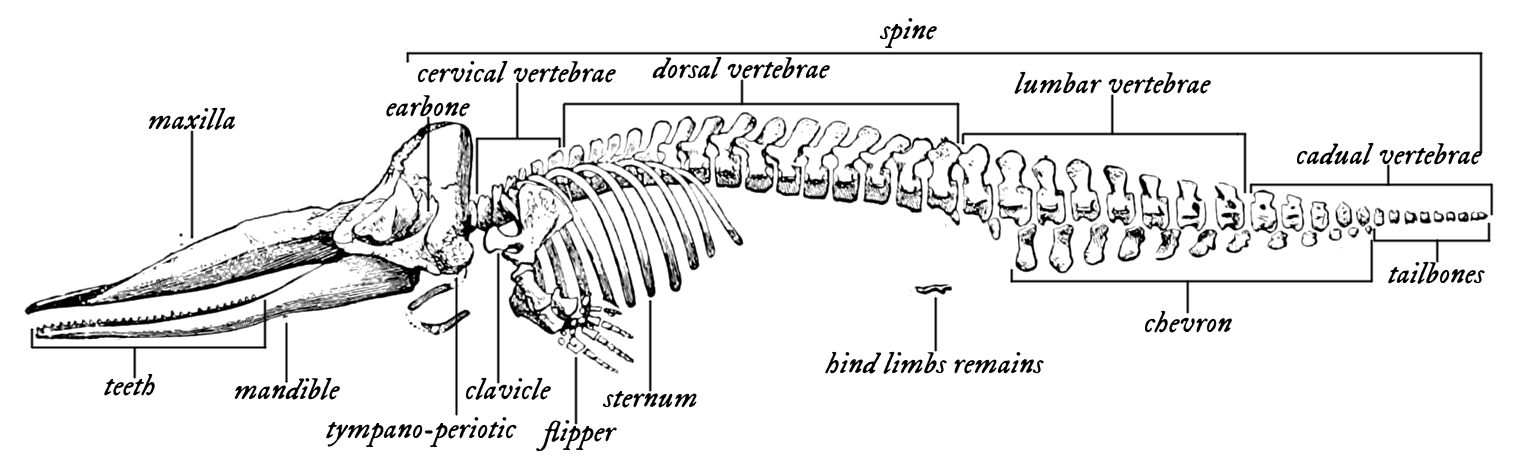
\includegraphics[width=0.99\textwidth]{01yuadrem/img/23sperm_whale_skeleton.png}
    \end{DndTable}
\end{table*}

\subsubsection{Wordbinding\\ \small{Dremshamad}}
Well known is the obsession of the many houses of Palegna with words, names, and languages, and evidence of this is wordbinding.
Wordbinding, or Dremshamad in dust tongue, is the art of giving strength to words so that, no matter the medium, their mere utterance conveys an tangible effect in the world.
Its spells are many and varied, like saving effects in scrolls or books to be invoked later, binding the will of creatures by using their true names, and speaking command words that can't be disobeyed by any mean.

Perhaps the most meaningful product of wordbinding are reflexive contracts.
These agreements bind through the strength of words alone, enforcing their terms upon the signing parties by tying harsh effects to the rights and duties specified.
Always produced in triplicate with each requiring three signatures per party, reflexive contracts are practically unvoidable, thus regarded as the perfect mean to ensure cooperation between beings, houses, or even entire nations.

% Crafting a document with words of power:
% * List of effects that can be produced (more are unlocked as expertise increases)
% * Interaction with words that produce such effect (spoken out loud, whispered, listened to, read)

% All contracts must have a clause that can void the contract by design. Most usually it is being burned by the fire of a wyrm, since this act is neigh impossible without dying.

\subsubsection{Windherding\\ \small{Dentrala}}
Perilous are the winds from the southern ocean, relentlessly tearing apart any ship that dares sail it's turbulent waters.
Many forget that the many tribes from the Qul archipelago had to deal with these strong winds and storms in their daily lives.
To face this, they slowly developed a complex system of sympathetic magic.

By standing atop large poles within eyesight of each other, ird witches from the dentralin tribe managed to stop the wind simply by holding their breath.
This practice gave rise to a wide array of wind-based spells that the tribe wise to use to their advantage during the tunsal wars, and eventually led to the establishing of Jenkash.

\subsubsection{Sigaldry\\ \small{Guen Tsue}}
Unlike other languages, the naenk tongue is deeply rooted in nature itself, and can be used to even directly talk to it, with seedspeech being the clear example.
This quality of the language led to Gannag's shamans to develop a writing system that can evoke effects when interacted with, called shinerunes.

The tsaneks of Gannag use this method to create self-triggering traps, which are set about villages to catch prey and ward off would-be invaders.
Apart from this, intricate shinerunes are used to many different effects, such as a silent bell alerting of the presence of a stranger in a dwelling, a self-heating plate to boil water in, or clothes that spontaneously heat up as a reaction to bad weather.
Truly, the capabilities of shinerunes are only limited by the creativity and skill of their author.

\begin{table*}[t]%
    \begin{DndTable}[width=\linewidth, header=\centering Knaenese Alphabet]{X}
        \centering
        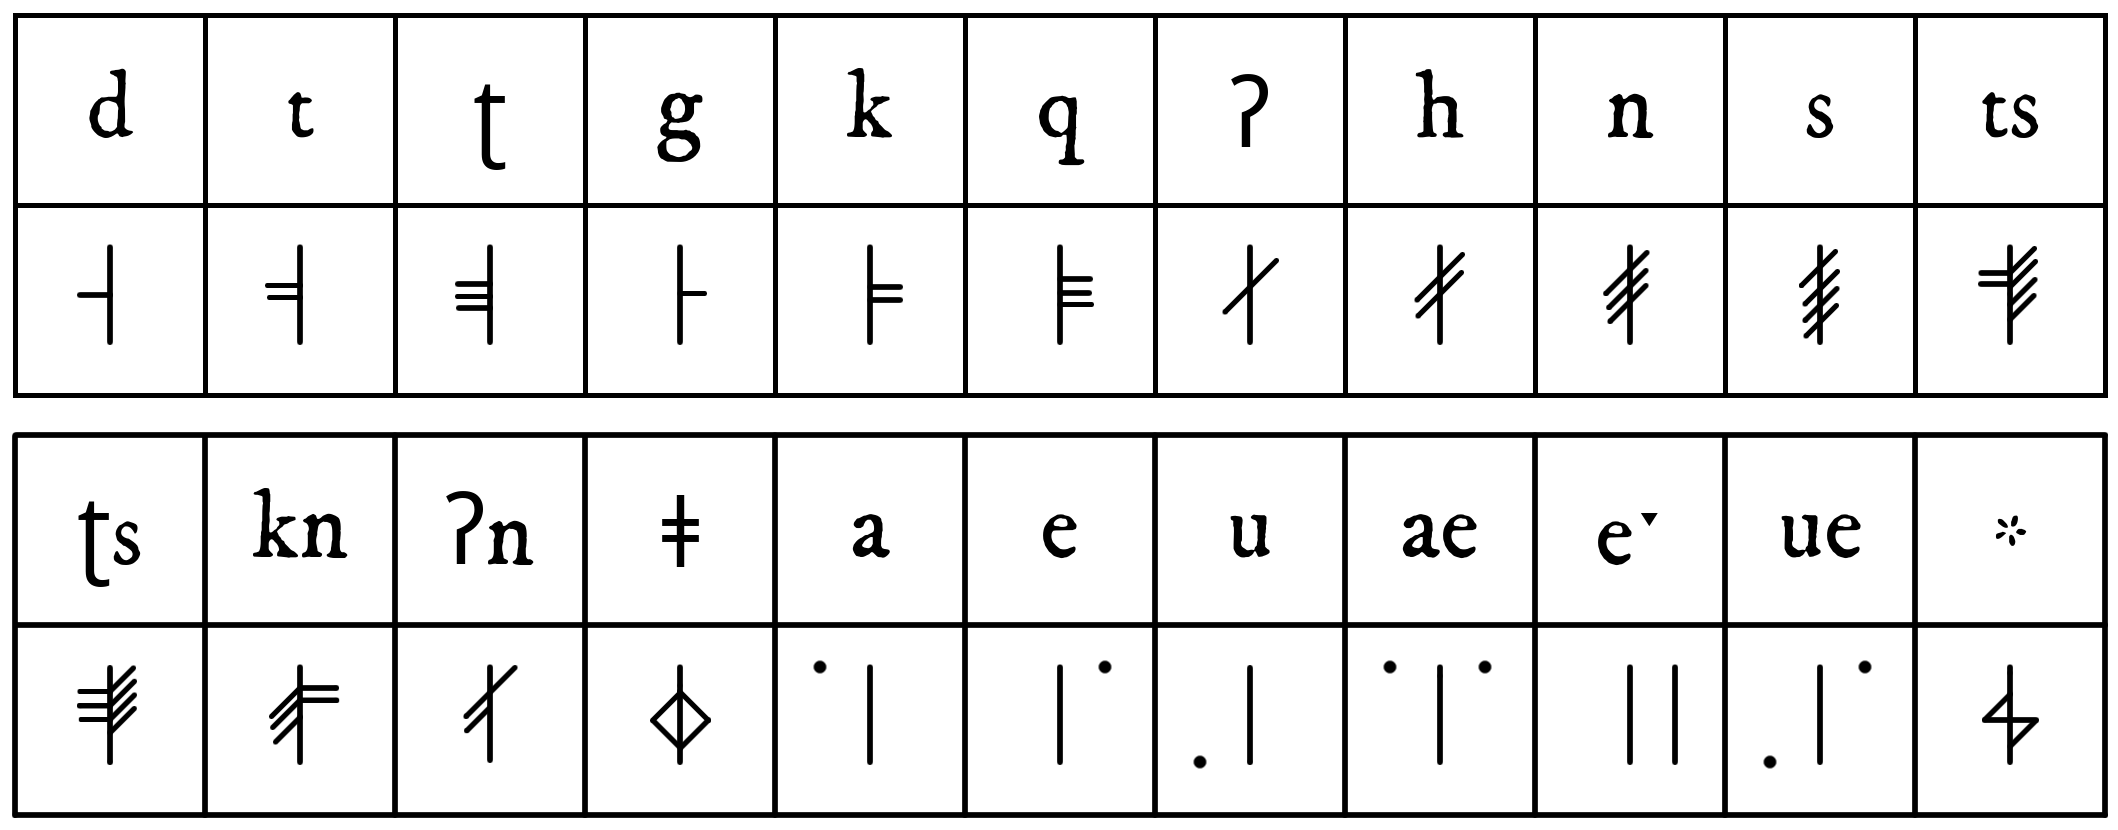
\includegraphics[width=0.99\textwidth]{01yuadrem/img/23knaenese_sample.png}
    \end{DndTable}
\end{table*}

\subsubsection{Psionics} % NOTE. I don't like the name but it's not that bad I guess.
Perhaps the strangest part of the zaloths is the fact that they do not speak through a mouth, but directly into other beings' minds.
This ability is only made possible by the special nature of the zaloths themselves, and is very rarely seen in the other kins, in peculiar gifted individuals.
Not limited to telepathy however, the art developed into a plethora of mind-based abilities known as psionics.

Psionics are fueled by one's own mind without external sources of energy, meaning that the art exerts a great effort from the author.
The zaloths have elaborated varied psionic effects to date, expanding their original telepathy to more tangible effects, like clairvoyance, telepathy, and many mind-altering effects.

\subsubsection{Similarity Sympathy}
% Blink (quantum teleport): Cantrip to teleport, only usable if being perceived by no sentient being when moving to an area not perceived by any sentient being. Hard to use in most cases yet extremely powerful in certain scenarios. (Mechanically it's a cantrip but using it is actually tiring, so it can't really be used as a reliable method of transportation).
% The best thaumaturges are blind FUCK YES!!

No one can deny that Yuadrem completely changed after the schism.
The ash storm ravaged the land and caused the 9 year famine, tens of thousands of strange creatures poured in, and new, alien kins settled into the land.
For better or for worse, the event transformed the fabric of reality.
Soon after the schism the witches and shamans of the early world started to experiment with a new and strange form of magic: the Similarity Link.

This link is a strange form of sorcery which seems to follow different rules than the other schools.
It affects directly the physical properties of objects and creatures, like making rocks weight as little as feathers, or changing the size of other creatures.
Perhaps the strangest part of this is that it seems to behave differently depending on if it's being perceived or not.%, and thaumaturges take advantage of this by covering their eyes when casting certain spells.

\subsubsection{Tidal Manipulation\\ \small{Rashid}} % !!
Rashid involves manipulating the tides in the air or in others to attain one's goals.
Originally taught by the sole survivor of the Rashiist school of thought, it ranges from simple charms and illusions to potent spells with effects that vary depending on the caster's or target's tidal alignment.

Every Rashid user knows that they must exercise their magic in secrecy, since the practice is severely punished due to Rashiism's dark history.
The most experienced in the art however know that the one they truly have to fear is the Sorrow.
The Sorrow is the being that destroyed the Rashiist school of thought, leaving the pale blemish as a warning to any who dares follow their teachings.

\subsubsection{Fleshshaping\\ \small{Cthai'khas}} % !!
Recently reborn in the breathing city of Cabb Goem-Rlamesh is the almost lost art of Ukarilth: fleshshaping.
An everyday act of the tall kin, fleshshaping is a kind of magic that involves transfiguring the flesh of the caster or of others nearby, be them alive or dead.

While most fleshshapers remain in their putrid island, some have started to show up in the eastern parts of Yuadrem, and the art is slowly being spread by concealed mages.
A strange attribute of fleshshaping that sets it apart from the other schools is that its effect vary depending on the species of the caster.
For example, while a gat can mold its flesh to temporarily use its bones as weapons, a naenk can grow roots into the floor to catch prey, and a quies can reinforce its wooden exterior in preparation for an attack.


% !TEX root = ../main.tex
\begin{figure}[H]
    \centering 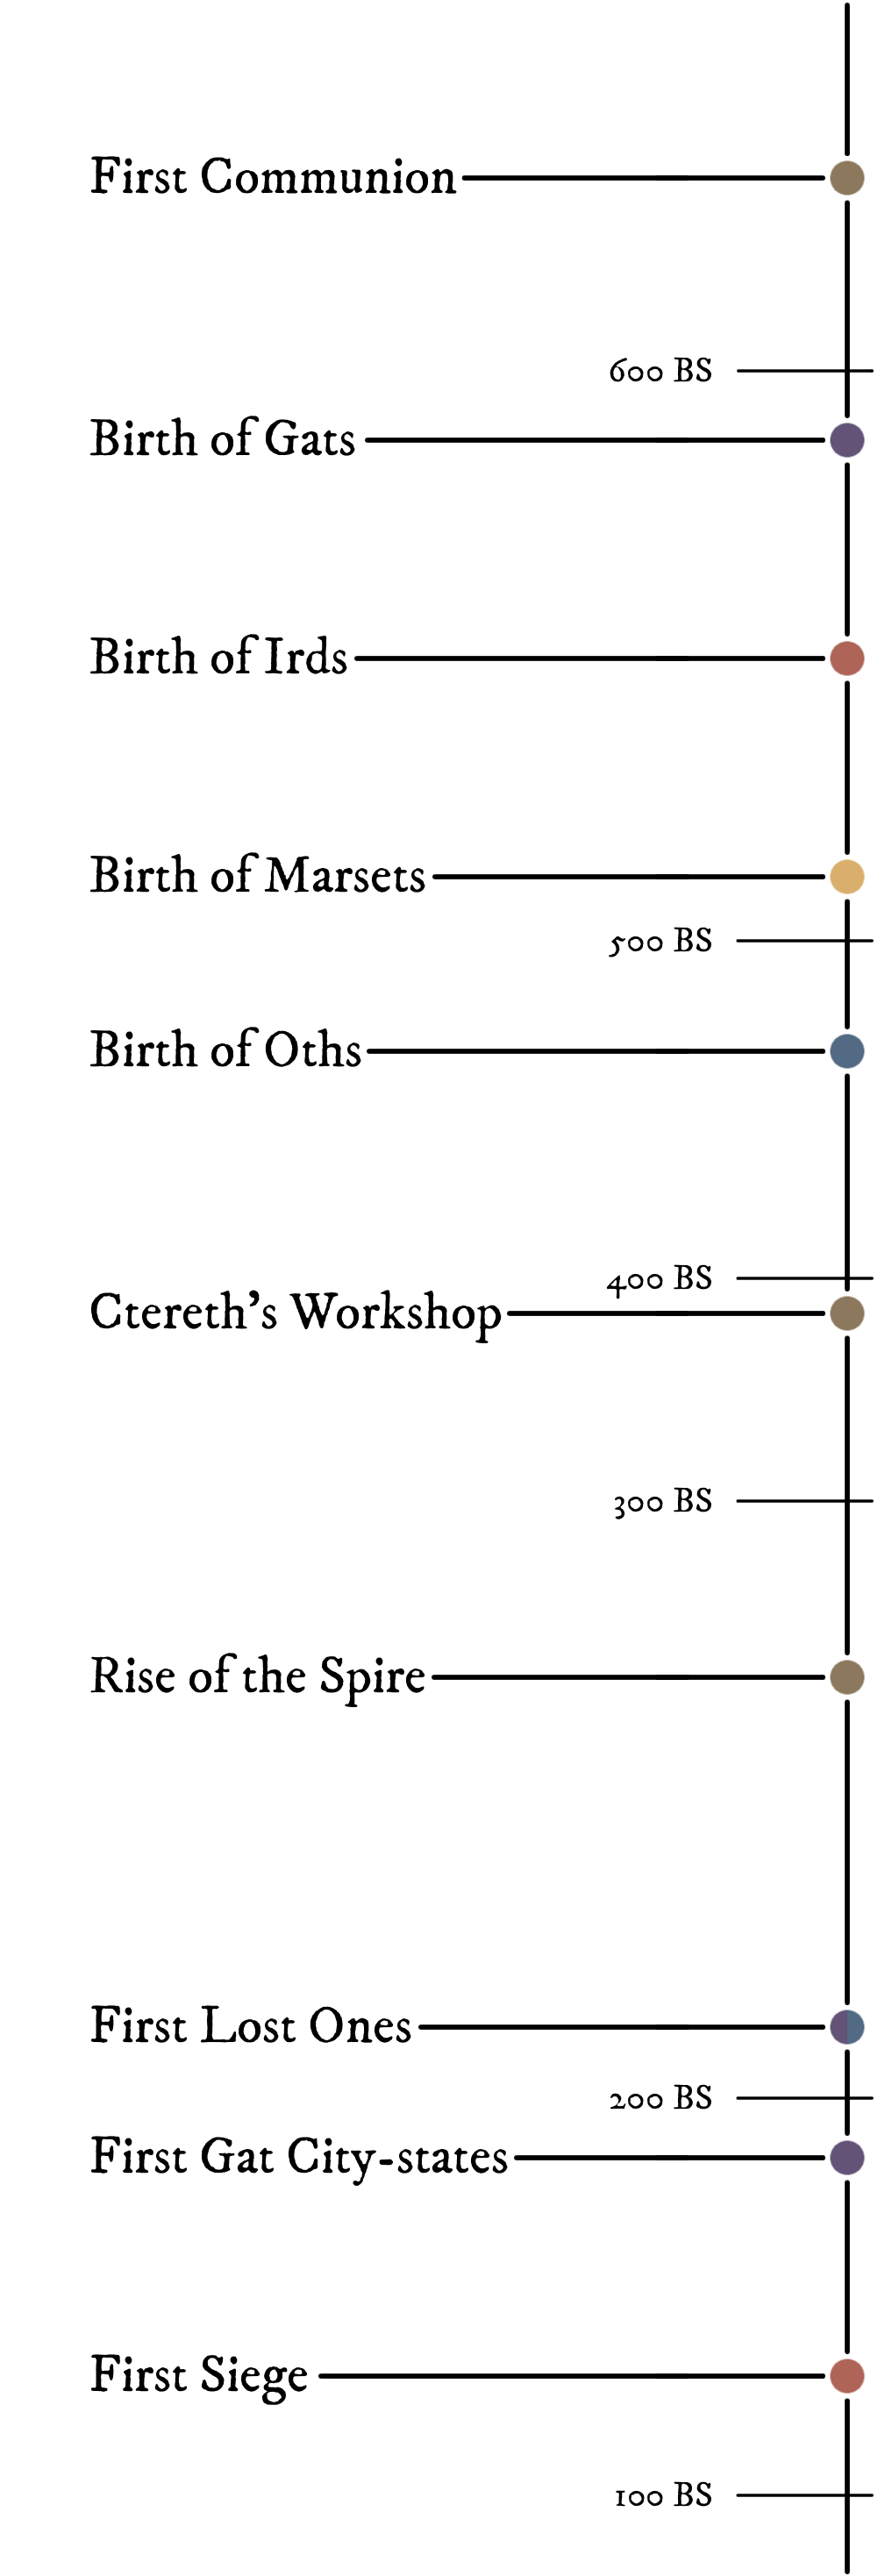
\includegraphics{01yuadrem/img/30history_i.png}
\end{figure}

\section{History} \label{sec::history}
% History is known in detail thanks to the dutiful oths that recorded it under Tol's guidance.
% TODO: Capitalise all the location names, like Arctic Archipelago, Sylvan Canyon, etc.
% TODO: Take a look at the whole cultures and Yuadrem pages and fix years and nation names!

\subsection*{Ancient History}
\subparagraph{682 BS --- First Communion} In the middle of the dead sea, the et E'ukarilth merges with a deceased higher one embryo.
This transforms the tall one into an insane visage of their former self.
The church of E'ukarilth is later founded to attempt communication with the et.

\subparagraph{592 BS --- Birth of Gats} The search for the Lung of Ur begins, an artifact of great value to the tall kin.
The indigo school of the et Thul-yharch creates the hardy gats, believing the relic is below the surface.

\subparagraph{547 BS --- Birth of Irds} With underground search proving unsuccessful, the red school of Zyl'rech births the mobile irds.
Taking to the skies, they survey land and ocean, hoping to find clues of Lung's location.

\subparagraph{523 BS --- Birth of Marsets} The gold school of Tosh-drieln produces the arboreal marsets.
They explore the thick and dark jungles of Yuadrem with ease.

\subparagraph{451 BS --- Birth of Oths} Under mysterious circumstances, oths are created by the et Tol.
Before disappearing, the tall one teaches them writing, and they begin recording history and compiling the findings of the ets and their progeny with great care and detail.

\subparagraph{397 BS --- Ctereth's Workshop} To cope with the uncontrolled population growth of the new kins, the et Ctereth digs a deep cavern in the middle of the dead sea.
Inside it, the tall one builds a workshop and tirelessly crafts qualar to gift the newborns sentience.

\subsection*{Nadir}
\subparagraph{217 BS --- The Rise of the Spire} The tall kin, apparently done with their search, create the spire at the place where E'ukarilth found the higher one.
They build the stone city of Jan'krug atop the mountain.
The progeny kins, now left alone, are forbidden from accessing the dead sea and, incapable of producing qualar, are forced to fight among themselves.

\subparagraph{209 BS --- First Lost Ones} The first plains gats and chu'ash oths are born, separated from their kins by their lack of qualar.
% While ird and marset lost ones also exist, the lack of a qualars doesn't affect these kins as much as their siblings, perhaps due to their wilder nature.

\subparagraph{179 BS --- First Gat City-states} The gats, always fighting adversity, establish the three city-states of Fiele, Avshen, and Alagyaz.
With careful birth control techniques, they manage to maintain a stable population.

\subparagraph{144 BS --- First Siege} A group of three irds known as ``the feathered sunrise'' infiltrates the dead sea and steal tens of thousands of qualar from Ctereth.
The nations of Krudzal, Harual, and Hulnar are later established by their descendants.

\begin{figure}[H]
    \centering 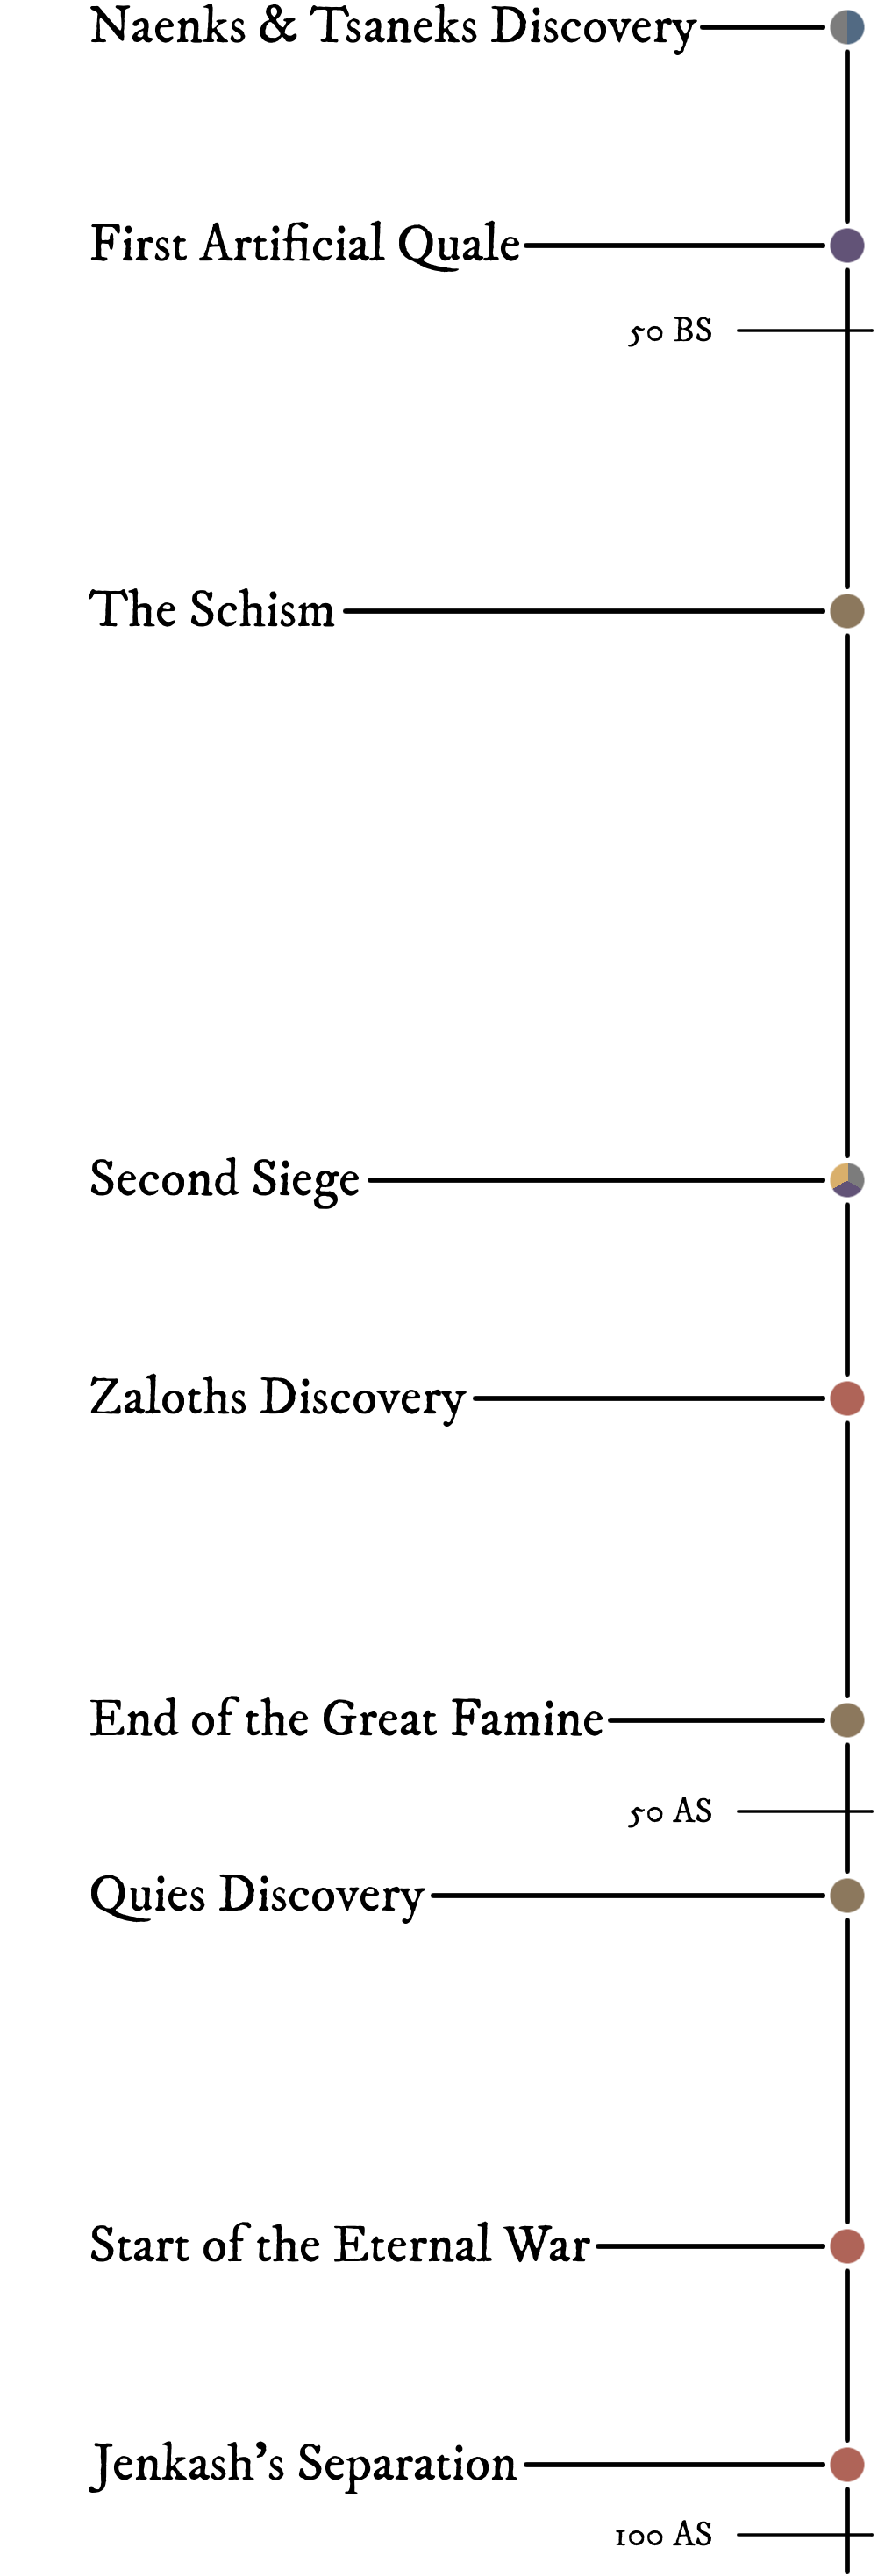
\includegraphics{01yuadrem/img/30history_ii.png}
\end{figure}

\subparagraph{92 BS --- Naenks \& Tsaneks Discovery} Trying to find a home, a group of stray marsets known as the Ovovians, stumble upon the naenks and tsaneks of Drejeck.
These two are inexplicable kins born from mold and fungi respectively.

\subparagraph{51 BS --- First Artificial Qualars} The gat Jirar the bonecarver creates a technique to craft rough qualars imitations.
By passing the practice to the gat's disciples, Jirar unshackles the population number of the kins, and boosts Alagyaz's economy to unprecedented levels.
% To date, only gat master bonecarvers have managed to use the technique. One bonecarver's qualar count usually doesn't go above the thousands, but as populations grow so does the need for qualar.

\subsection*{Great Famine}
\subparagraph{0 --- The Schism} The tall kin's folly causes the schism.
The spire, now revealed to be a dormant volcano, catastrophically erupts.
The event destroys Jan'krug and most of the ets.
The spewed ash blocks off sunlight for four decades, starting the age known as the great famine.

The explosion causes a portal known as the sizzling gate to be opened in a cave inside of the spire.
This door leads to the outer lands, a strange and primal plane that exists outside of Yuadrem.
From the portal spew forth the foreigner kins: the adventurous tortles, the violent grungs, and the ingenious umans, along with the blueblood beasts.

\subparagraph{1 AS --- Second Siege} The foreigner's horde, a great army of tortles, grungs, and umans, siege Ctereth's workshop.
They're successful, and the great number of qualar stolen is used to start their own settlements in Yuadrem.

\subparagraph{4 AS --- Zaloths Discovery} The zaloths, a kin made of fire, ash, thunder, and hail, walk down from the ruins of Jan'krug.
They freely roam Yuadrem, following a nomadic lifestyle that keeps most away from civilized society.

\subsection*{Age of Heroes}
\subparagraph{38 AS --- End of the Great Famine} Satisfied with a death toll in the tens of millions, the ash clouds from the spire disperse, finally ending the great famine.

\subparagraph{57 AS --- Quies Discovery} A group of gat voyagers from Avshen rise up to Jan'krug, finding the city ruined beyond repair, covered by solidified lava.
However, what they do find beneath the ruins are the quies, a new kin.
Quies are the last kin created by the ets, and are brought back to Avshen.
They easily integrate into gat society, despite their physical differences.

\subparagraph{71 AS --- Start of the Eternal War} The newly born kingdom of Krudzal in the north begins a war against the stone giants of the northern territories.
The war rages to this day, with little obtained by the thul'kraka irds.

\subparagraph{99 AS --- Jenkash's Separation} A blossoming nation of qulbaba irds is split into forty-five separate tribes by ideological differences.

\begin{figure}[H]
    \centering 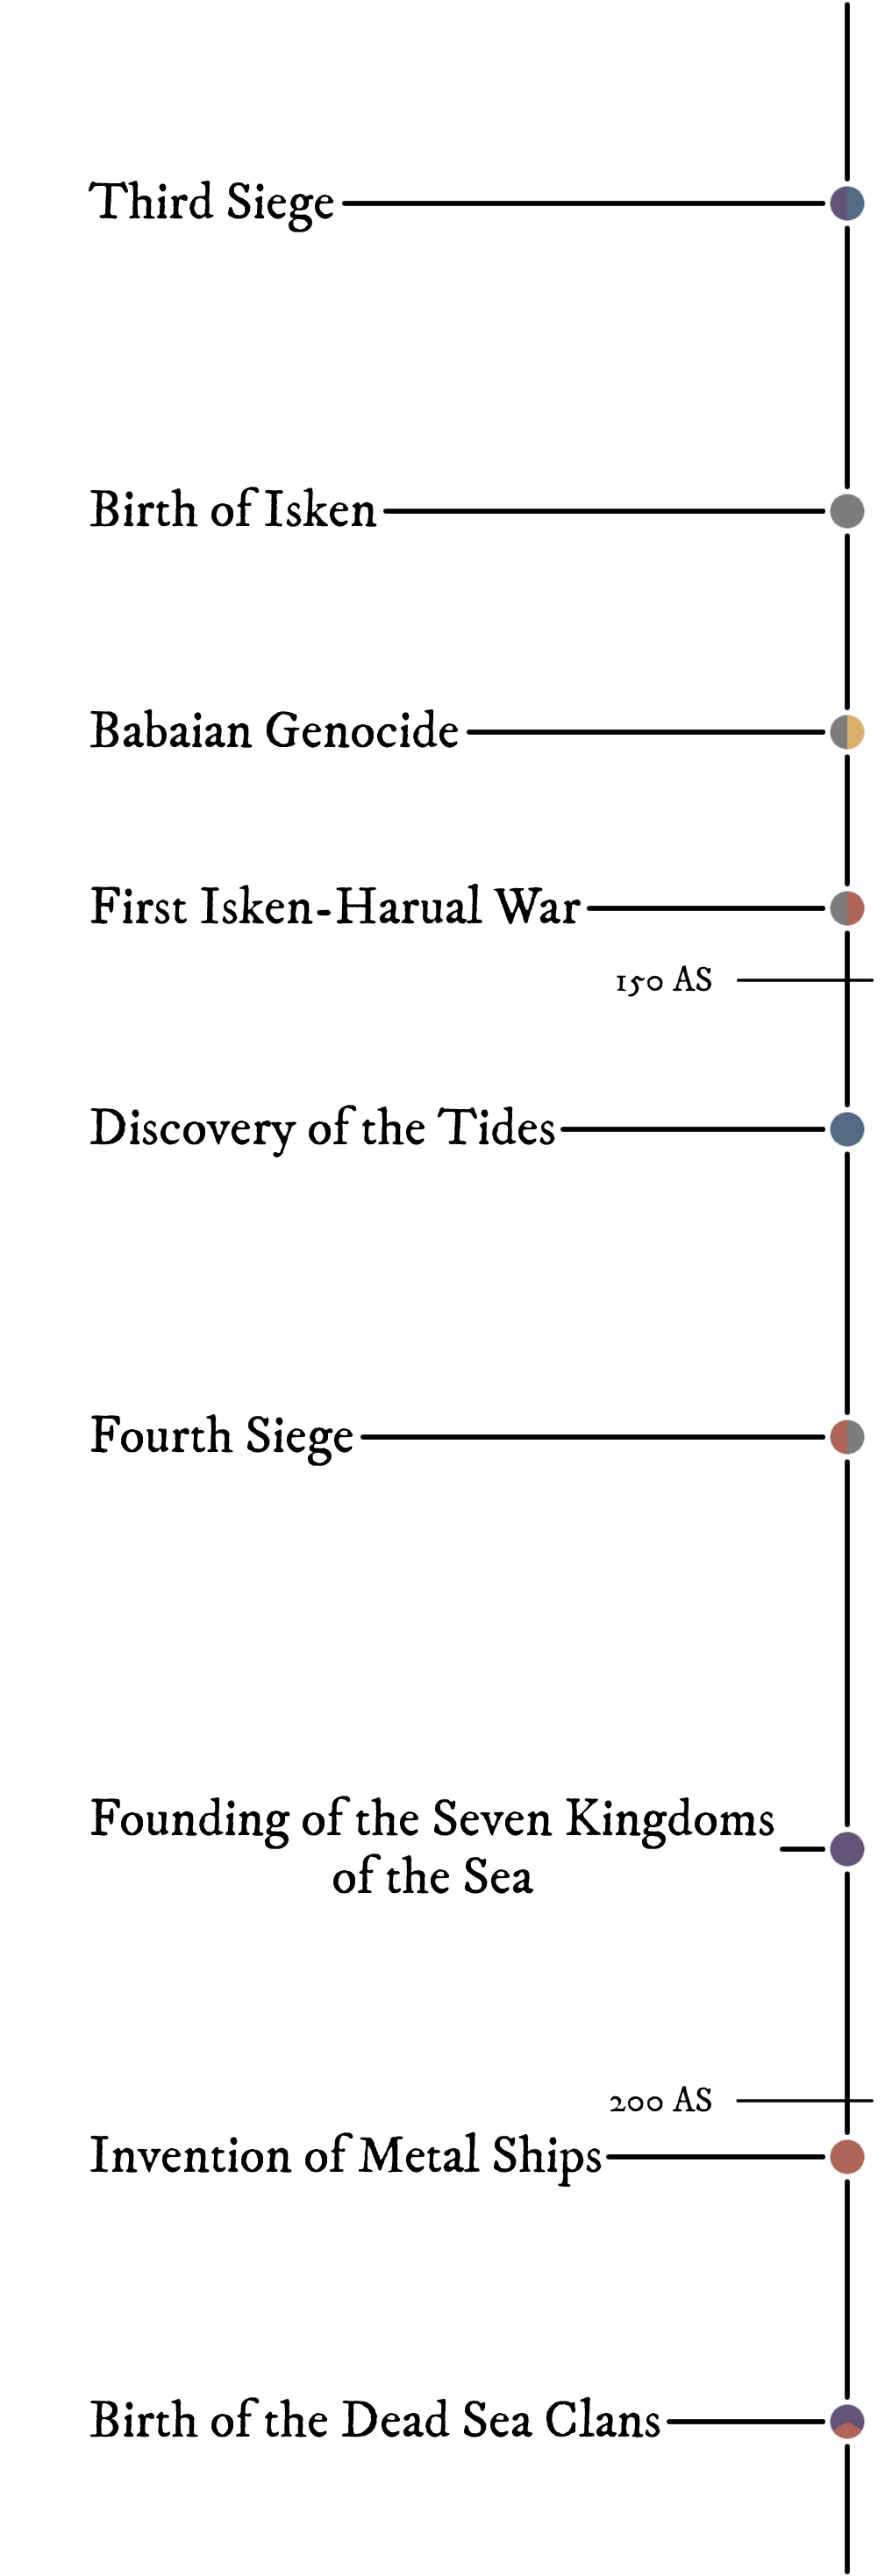
\includegraphics{01yuadrem/img/30history_iii.png}
\end{figure}

The tribes that will eventually become Jenkash are bound to constant conflict, unable to establish a unified government for more than a hundred years.

\subparagraph{102 AS --- Third Siege} Inspired by their siblings lost three centuries ago, the army of healing is formed.
Mainly composed of gats and oths, they successfully invade Ctereth's dwellings, then personally bringing the stolen qualar to the bughna gats and the chu'ash oths, re-integrating them into civilized society.

\subparagraph{141 AS --- Birth of Isken} Among the dark forests of the Chirping Wilds, the grung empire of Isken is formed.
Initially secretive, they will soon become one of the most fearsome forces in Yuadrem.

\subparagraph{143 AS --- Babaian Genocide} The grungs of Isken easily crush the marset nation of Baba, systematically killing the marsets until very few are left.

\subparagraph{144 AS --- First Isken-Harual War} Ever hungry for power and land, the Iskean empire attacks the Harualish tribes of the Chirping Wilds.
This is the start of a long sequence of slow and bloody wars that will last for more than two centuries.

\subparagraph{174 AS --- Discovery of the Tides} The oths from the temple of Ignelli, led by Hashim, unearth the phenomenon of the tides, learning of its influence on the kins of Yuadrem.
The discovery revolutionizes the way the kins perceive their own feelings and motivations, and leads to them questioning the nature of sentience itself.

\subparagraph{189 AS --- Fourth Siege} To cope with their ever-growing populations, a temporary alliance is formed between the dratl ird houses of the west and the grung empire of the east.
Their union leads to the fourth and final successful siege of Ctereth, enabling a great growth for the Hulnar and Iskean empires.

\subsection*{Age of Nations}
\subparagraph{195 AS --- Founding of the Seven Kingdoms of the Sea} Ever-growing in numbers, the gat city-states coasting the whaler's sea coalesce into nations, each under its own king.
With all the events happening in one year, the formation of the seven kingdoms of the sea initiate an age of prosperity for the horned and retainer kins.

\subparagraph{201 AS --- Invention of Metal Ships} Edren, a thul'kraka ird from Krudzal, designs and invents the first ironclad ship.
The design, named after the ird's son, Durkin, boosts Krudzal's trading capabilities and kick-starts a great colonization campaign.

\subparagraph{212 AS --- Birth of the Dead Sea Clans} Imitating their neighbors to the north, many uman, dratl ird, and plains gat clans are established in the dead sea.

% These clans however are very different from the civilized kingdoms of the north.
% Warlords are elected by strength, and their territories are as shifting as the erratic sandstorms.

\begin{figure}[H]
    \centering 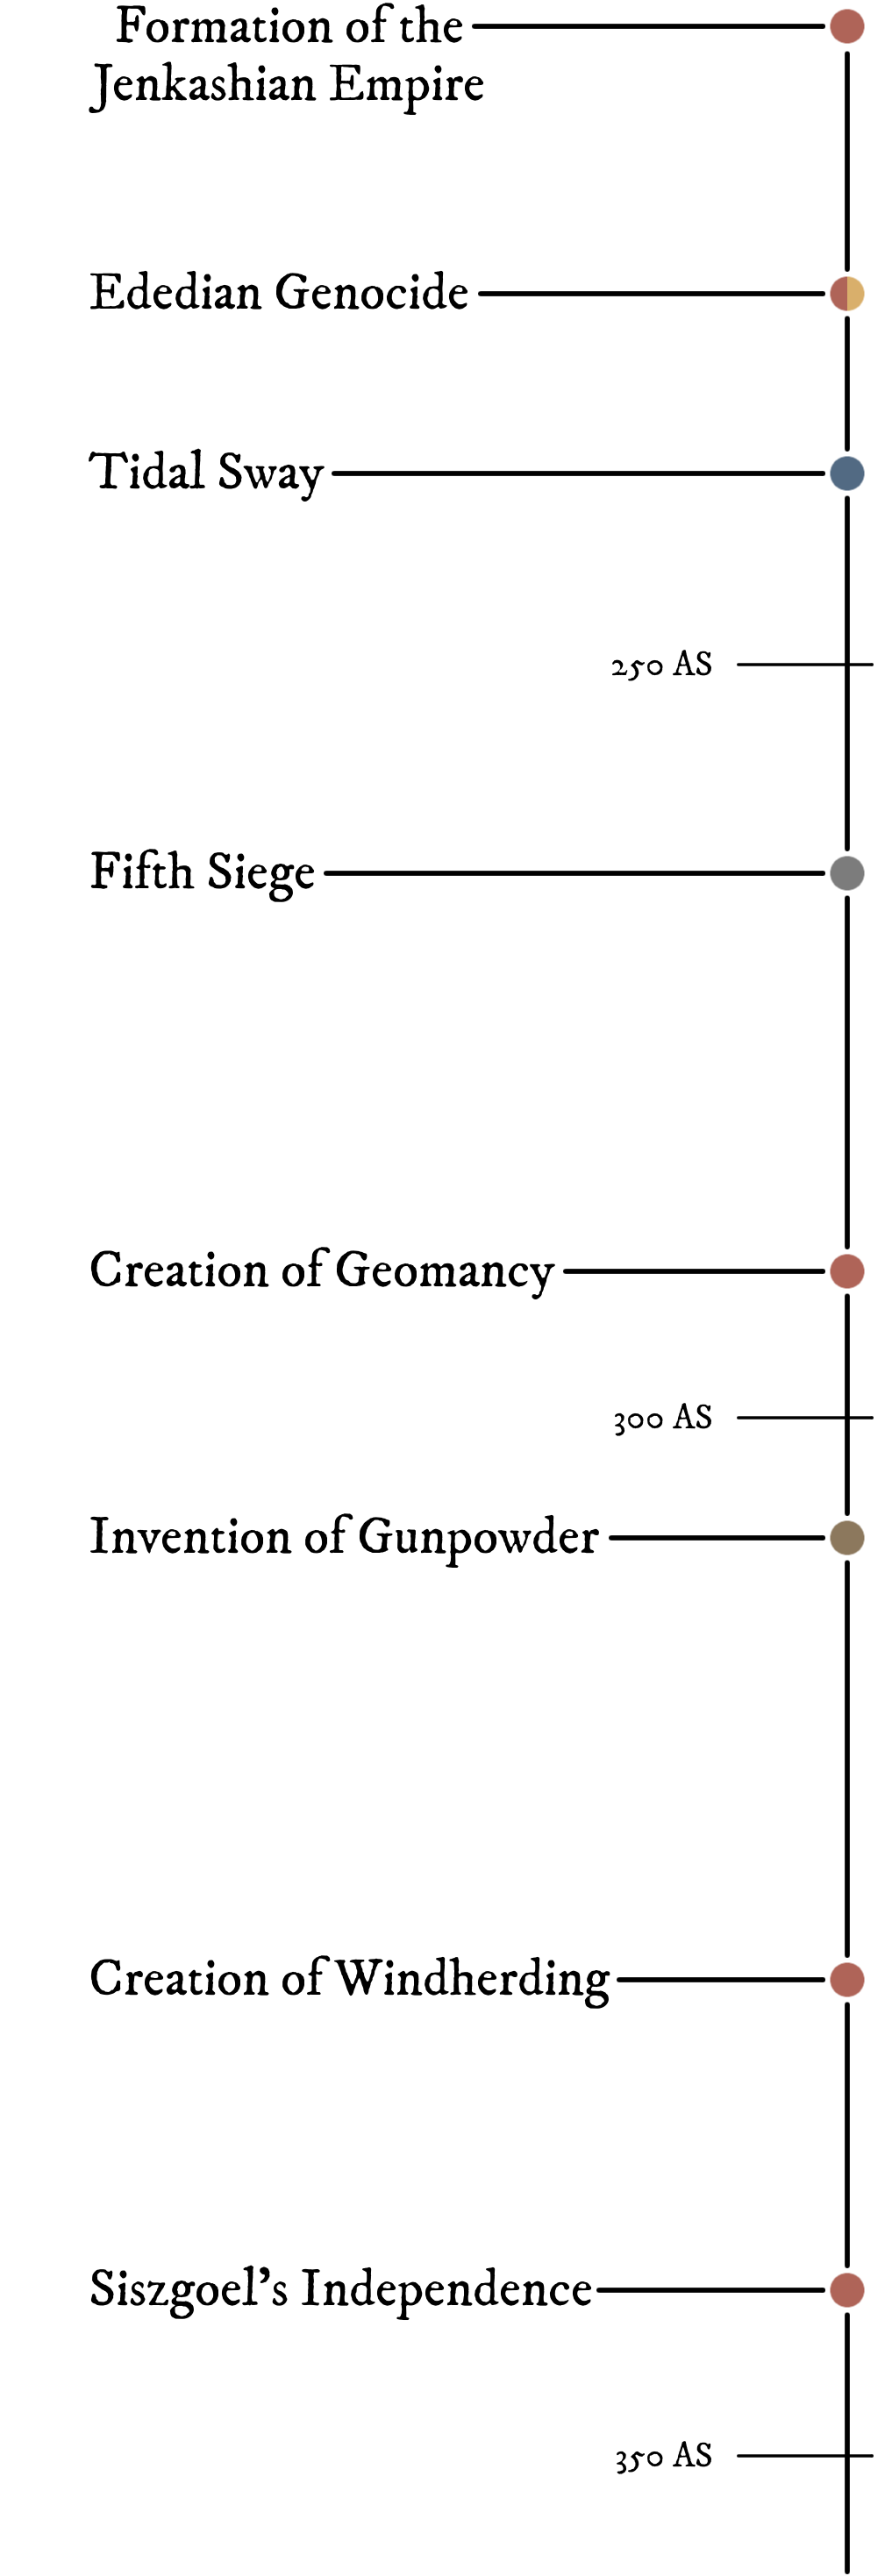
\includegraphics{01yuadrem/img/30history_iv.png}
\end{figure}

\subparagraph{229 AS --- Formation of the Jenkashian Empire} Driven by inner conflict, the irds of the qul archipelago exhaust their natural resources.
This forces them to prematurely end their quarrels, and begin invading and pillaging the surrounding territories.

\subparagraph{231 AS --- Ededian Genocide} The Springwater island is almost completely overtaken by Jenkash, decimating the marset population and forcing most into exile.

\subparagraph{247 AS --- Tidal Sway} Hailing from Ignelli, the oth Narr from the Rashiist school of thought performs an uncanny ritual to harness the power of the tides.
This accidentally triggers the tidal sway.

The oth summons the Sorrow into Yuadrem, ending the life of most Rashiists and ravaging the wildlands entirely, blocking access by land to the southern regions of Yuadrem.

\subparagraph{272 AS --- Fifth Siege} The Iskean grungs, banned from buying artificial qualar from Khedrat, attempt a new siege upon Ctereth's workshop.
This time however they fail, stopped by an unsuspected force: the newly formed dead sea clan of Dzarog.
Dzarog is a clan of umans and gats that live in dens around the spire, and protect Ctereth's caverns for yet unknown reasons.

\subparagraph{281 AS --- Creation of Geomancy} The ird nation of Hairuus, protected from Isken by the splitting mountain range, develop the art of geomancy.
As a test of their mastery of it, they elevate an island at the middle of the shield lake, where their capital, the Nest, is built.

\subparagraph{304 AS --- Invention of Gunpowder} Hailing from the young nation of Sulia, the oth Karmin discovers gunpowder.
With this new firepower, many engineers from Sulia design and build varied weapons, like fire spears, hand-cannons, and muskets.
These new weapons give them a proper combat advantage, allowing them to defend themselves from the savage nomadic tribes of the blank plains, and slowly expand their territories to the east.

\subparagraph{331 AS --- Creation of Windherding} The uncommonly peaceful irds from the Dentrala tribe in Jenkash develop the art of windherding.
The other tribes quickly adapt this art for combat, leading to the Drejeck wars against the naenks of Gannag and the Dratl'fal wars against the declining empire of Hulnar.

\subparagraph{340 AS --- Siszgoel's Independence} Siszgoel, a long-standing colony of Krudzal, declares independence.
The nation of Kaldrathal is born, under the rule of the warrior queen Ialul.
The natural deposits of nitrate in the country's island of residence, Krejek, boosts a powerful gunpowder industry, quickly matching that of Sulia.

\begin{figure}[H]
    \centering 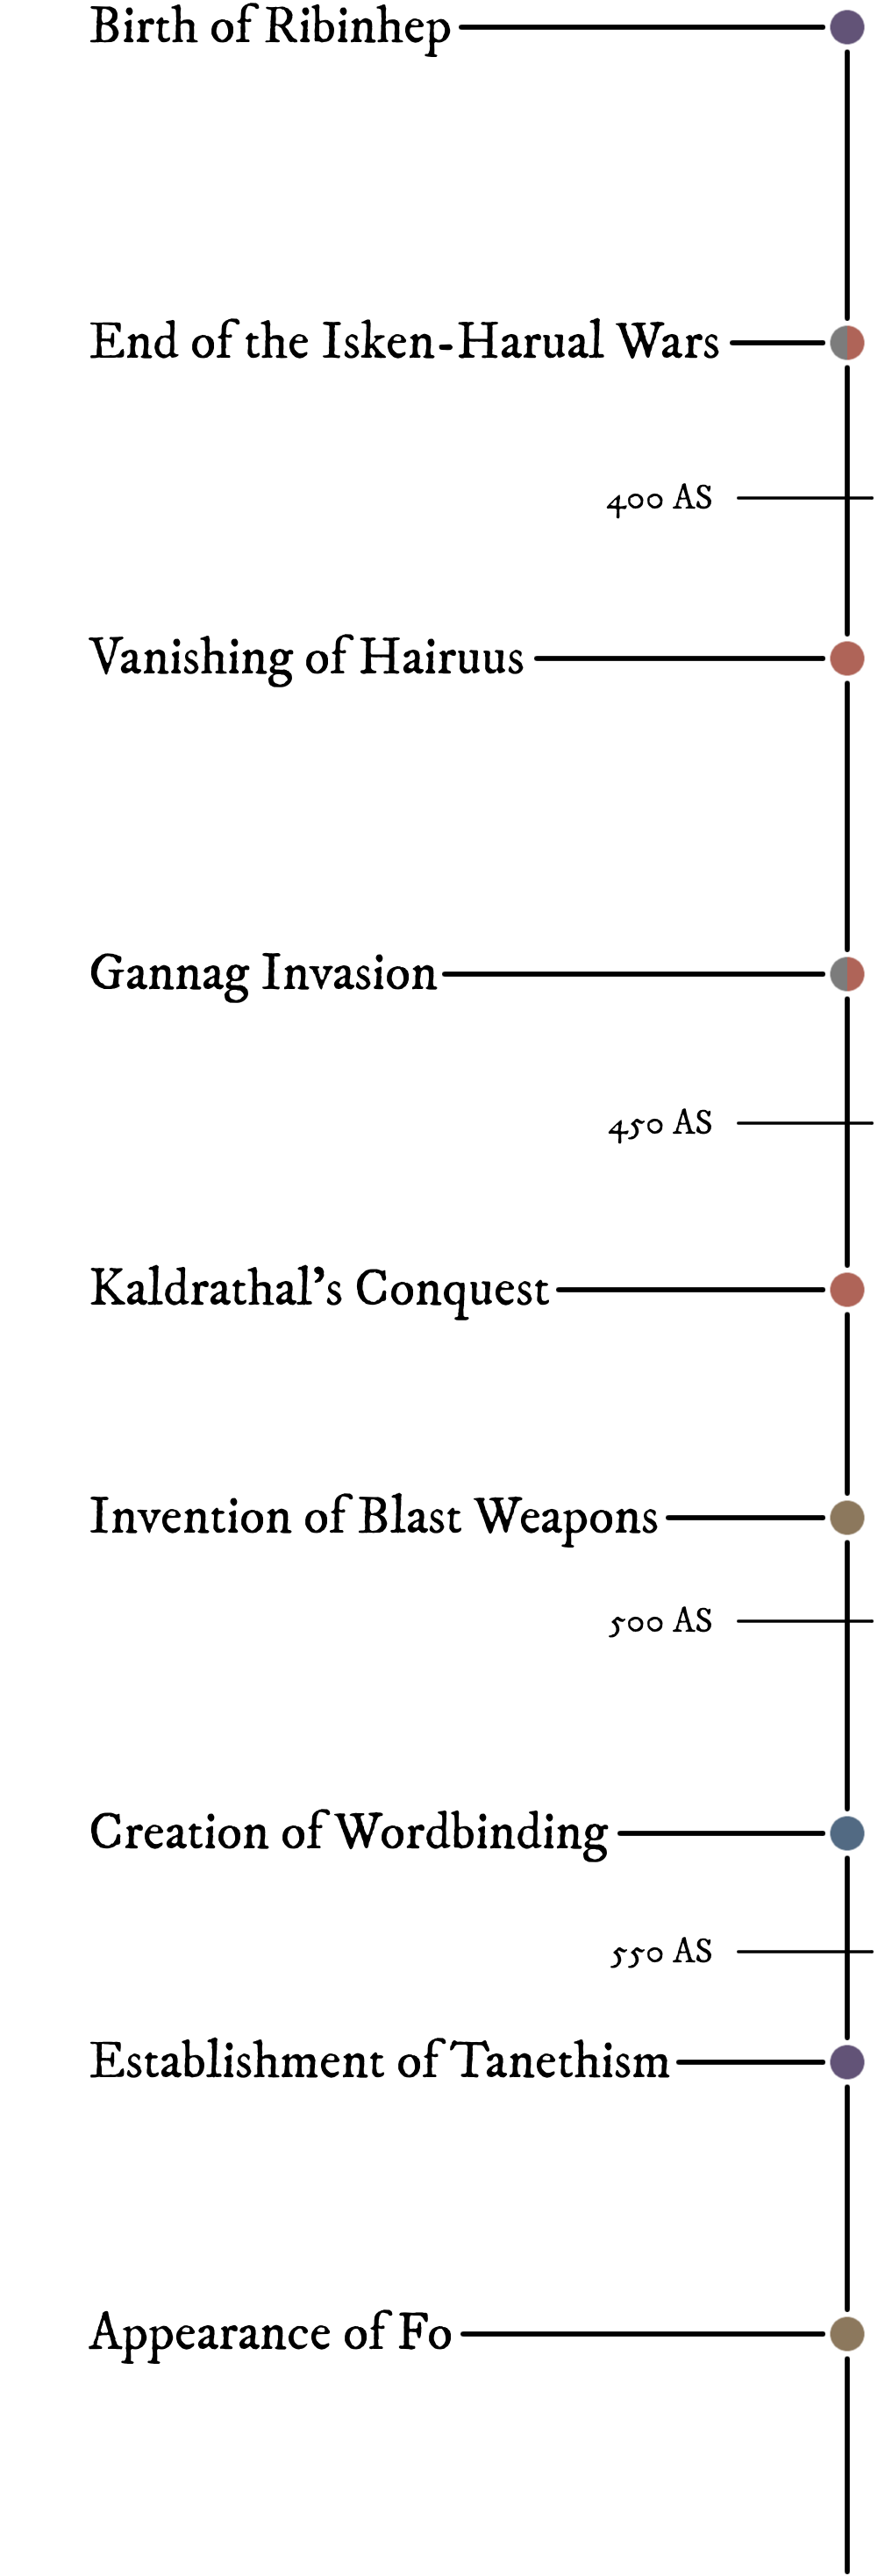
\includegraphics{01yuadrem/img/30history_v.png}
\end{figure}

\subparagraph{354 AS --- Birth of Ribinhep} Umans, a kin commonly hunted an enslaved, manage to establish permanent settlement in the isle of rust.
Naming themselves Ribinhep, they start conquering the northern fjords using their unique mercury weapons, fighting under the rule of the frostburn king Kuin.

\subparagraph{389 AS --- End of the Isken-Harual Wars} After 248 years, the Isken-Harual wars end, with Isken crushing almost all of the ird tribes.
The grung empire quickly proceeds to attack the Byurev nation, attempting to conquer territories up north.
They are however stopped by the gats, prepared for such an invasion decades ago.

\subparagraph{411 AS --- Vanishing of Hairuus} The lake-based country of Hairuus suddenly vanishes, soon after elevating new land for their growing capital.
Rumors that the lake is haunted begin spreading, and nations avoid claiming the empty territories and abandoned cities for fear of this mysterious curse.

\subparagraph{440 AS --- Gannag Invasion} Seeing that the Jenkashian forces are focused on conquering the mainland, the armies of Gannag suddenly invades the qul archipelago under the command of Kutsa the sharp.
In few weeks they manage to conquer half of Jenkash's homeland, taking prisoner irds as sacrifices to use as birth corpses.

\subparagraph{461 AS --- Kaldrathal's Conquest} Most of the islands of the arctic archipelago are claimed by Kaldrathal, who establishes a new form of government that tries to represent the taken territories.

\subparagraph{498 AS --- Invention of Blast Weapons} Reut, an engineer from Drer, invents a new use of Sulia's gunpowder: Blast weapons.
Used for close-quarters combat, blast weapons aim to both surprise and immolate the enemy.
Among the most famous examples are the flame vent, the firecrackers and the flaming pole-arms.

\subparagraph{533 AS --- Creation of Wordbinding} In collaboration, the many oth houses of Palegna create the art of wordbinding.
The technique quickly gains traction, as it adds a method for trustless trade between peoples and nations.

% \subparagraph{553 AS --- Na'ane's Founding} A large circle of tsaneks led by Tsehant, tired of their class-based society, made a pilgrimage to the fog gorge.
% They establish in it, and form the independent nation of Na'ane.

\subparagraph{577 AS --- Establishment of Tanethism} The king of Khedrat, Grigor the Old, establishes the recently born Tanethism as the official religion of the nation.
The other kingdoms of the sea follow soon after, and Tanethism is quickly adopted by most gats.
% Here is when bonereading becomes accepted in the seven kingdoms.

\subparagraph{589 AS --- Appearance of Fo} Strange, twisted creatures start attacking any village coasting the shield lake, causing havoc.
Fo, the kinless inhabitant of the nest is quickly blamed for the creation of this creatures, but all attempts to reach the being have failed.

\begin{figure}[H]
    \centering 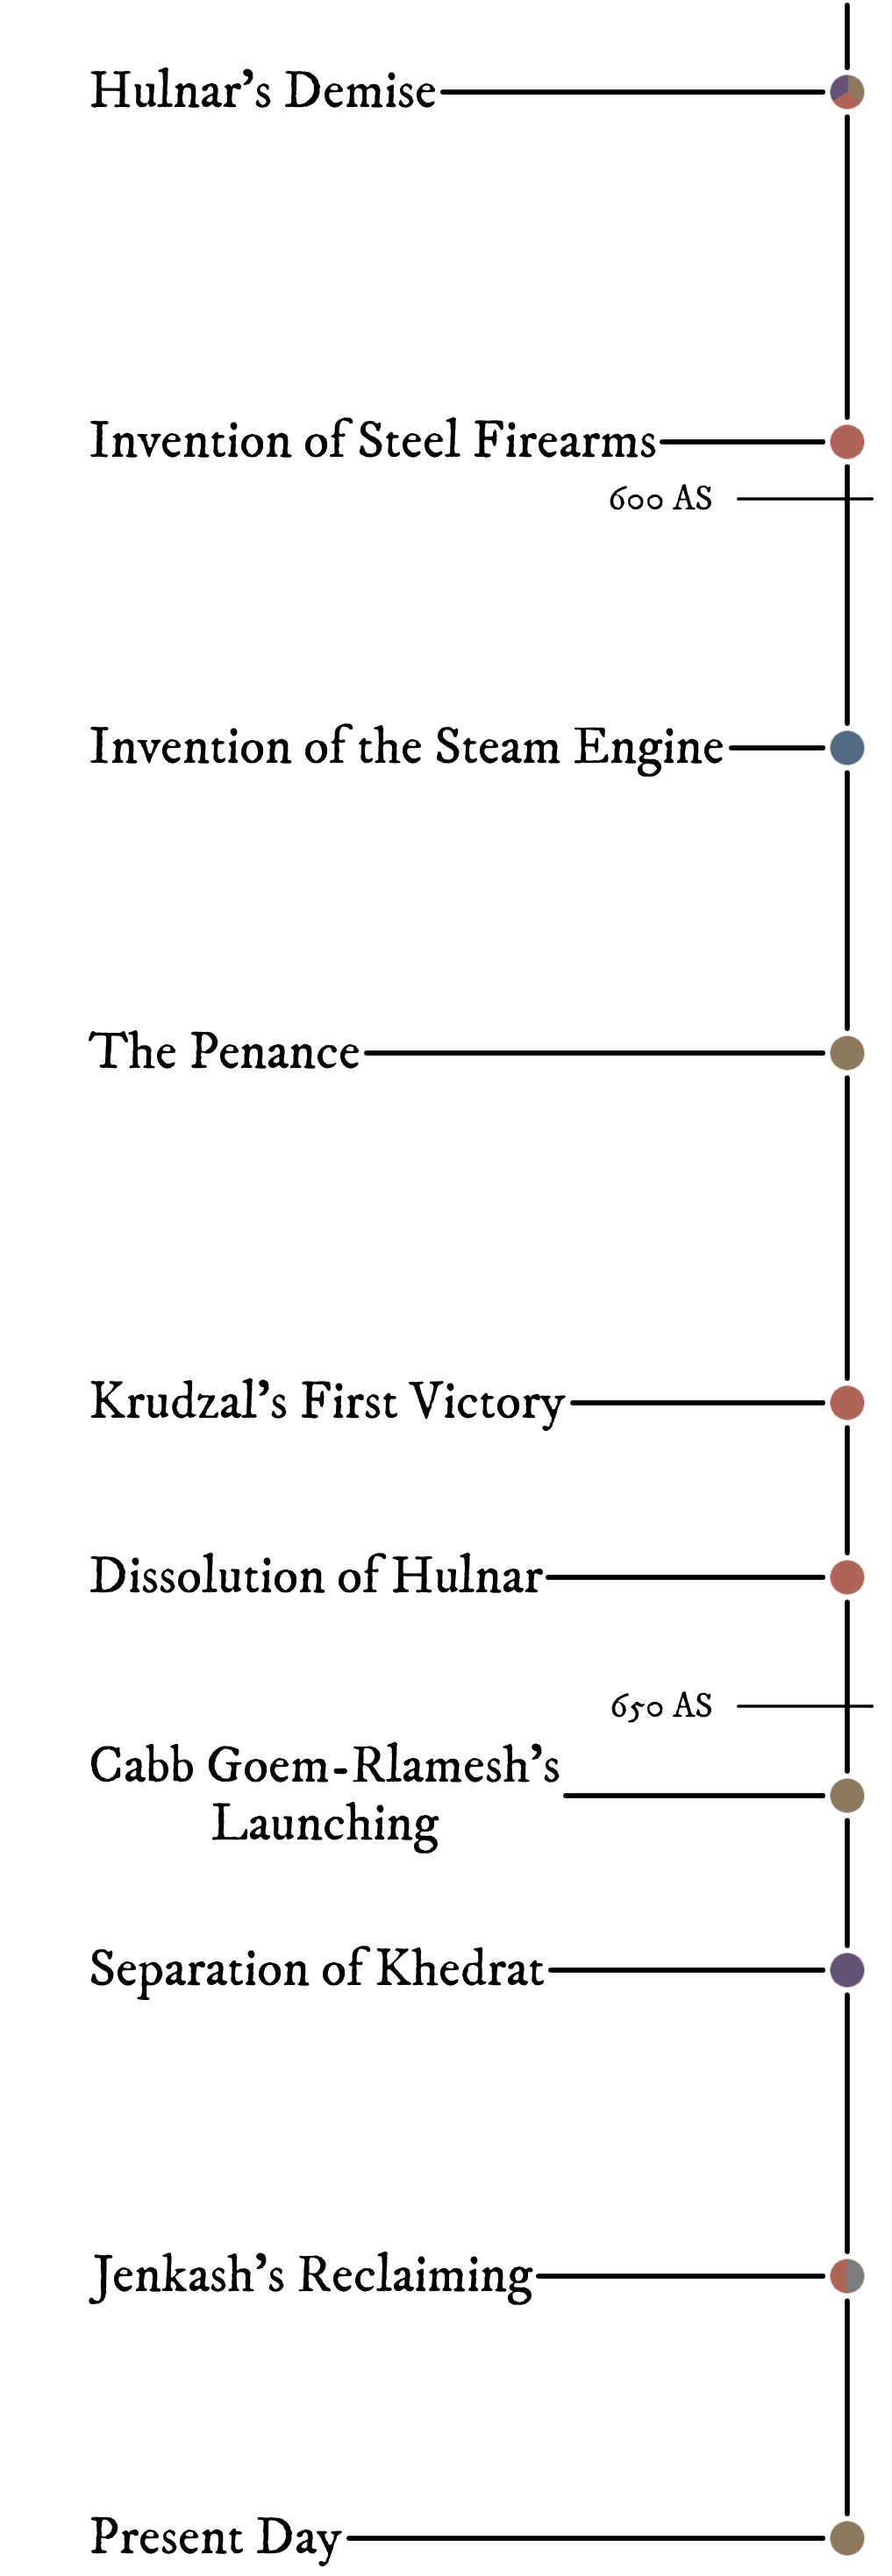
\includegraphics{01yuadrem/img/30history_vi.png}
\end{figure}

\subsection*{Golden Age}
\subparagraph{591 AS --- Hulnar's Demise} The strong alliance between the nations of Khedrat and Sulia defeats Hulnar in the Sylvan wars, allowing both nations to occupy a segment of the Ichor mountains and the entirety of the Sylvan canyon.
This act helps mitigate the pirates' presence in the Whaler's Sea, kick-starting an era of peace and trade for the coastal nations.

\subparagraph{599 AS --- Invention of Steel Firearms} The inventive Kaldrathian engineer Seja combines Krudzal's quench-hardened steel with her new refined gunpowder.
The explosive mix leads to the development of fierce steel-based weapons, including long-range cannons, wheel-lock pistols and sophisticated rifles.

\subparagraph{607 AS --- Invention of the Steam Engine} Away from the economic center of Yuadrem, the Na'anian tsanek Nugut invents the steam engine.
Originally used simply to drain the Na'anian coal mines, the tsaneks were quick to notice its potential and found hundreds of applications for the engine over time.

\subparagraph{621 AS --- The Penance} A surreptitious ritual known only as ``The Penance'' is carried by the citizens of Dzarog.
From the top of the spire, they summon a horrible being known as Cabb Goem-Rlamesh into Yuadrem.
The colossal amalgamate of flesh slowly drags itself towards the east, ferociously protected by the Dzarogian armies.

\subparagraph{628 AS --- Krudzal's First Victory} Using modified Kaldrathal cannons, Krudzal finally manages to kill a stone giant, claiming their first victory in the Eternal War.
% The event strikes fear on the giants, and Krudzal manages to claim their first territories in the mainland.

\subparagraph{635 AS --- Dissolution of Hulnar} Heirless, the king Sul'rech of Hulnar suddenly dies at a young age.
The dwindling kingdom is split into smaller houses, weak ghosts of Hulnar's old glory.

\subparagraph{655 AS --- Cabb Goem-Rlamesh's Launching} The harrowing immensity, Cabb Goem-Rlamesh, reaches the Burnt Ocean and settles some kilometers off the coast of the dry savanna.
% It becomes known as the breathing city.
% All expeditions to the island have ended poorly.

\subparagraph{659 AS --- Separation of Khedrat} The newly-conquered westernmost territories of Khedrat quickly become tired of monarchy, and peacefully claim independence.
Abandoning old traditions, the new countries of Viphogher and Dnomit embrace democracy: a new, king-less form of government.

\subparagraph{671 AS --- Jenkash's Reclaiming} Forced by Gannag to halt their conquest, the Jenkashian empire focused entirely on re-taking the qul archipelago.
Savage battles are fought, and to date they've managed to reclaim most of their lost homeland.

\subparagraph{672 AS --- Present Day}
\newpage

% !TEX root = ../main.tex
% \begin{figure}[H]
%     \centering 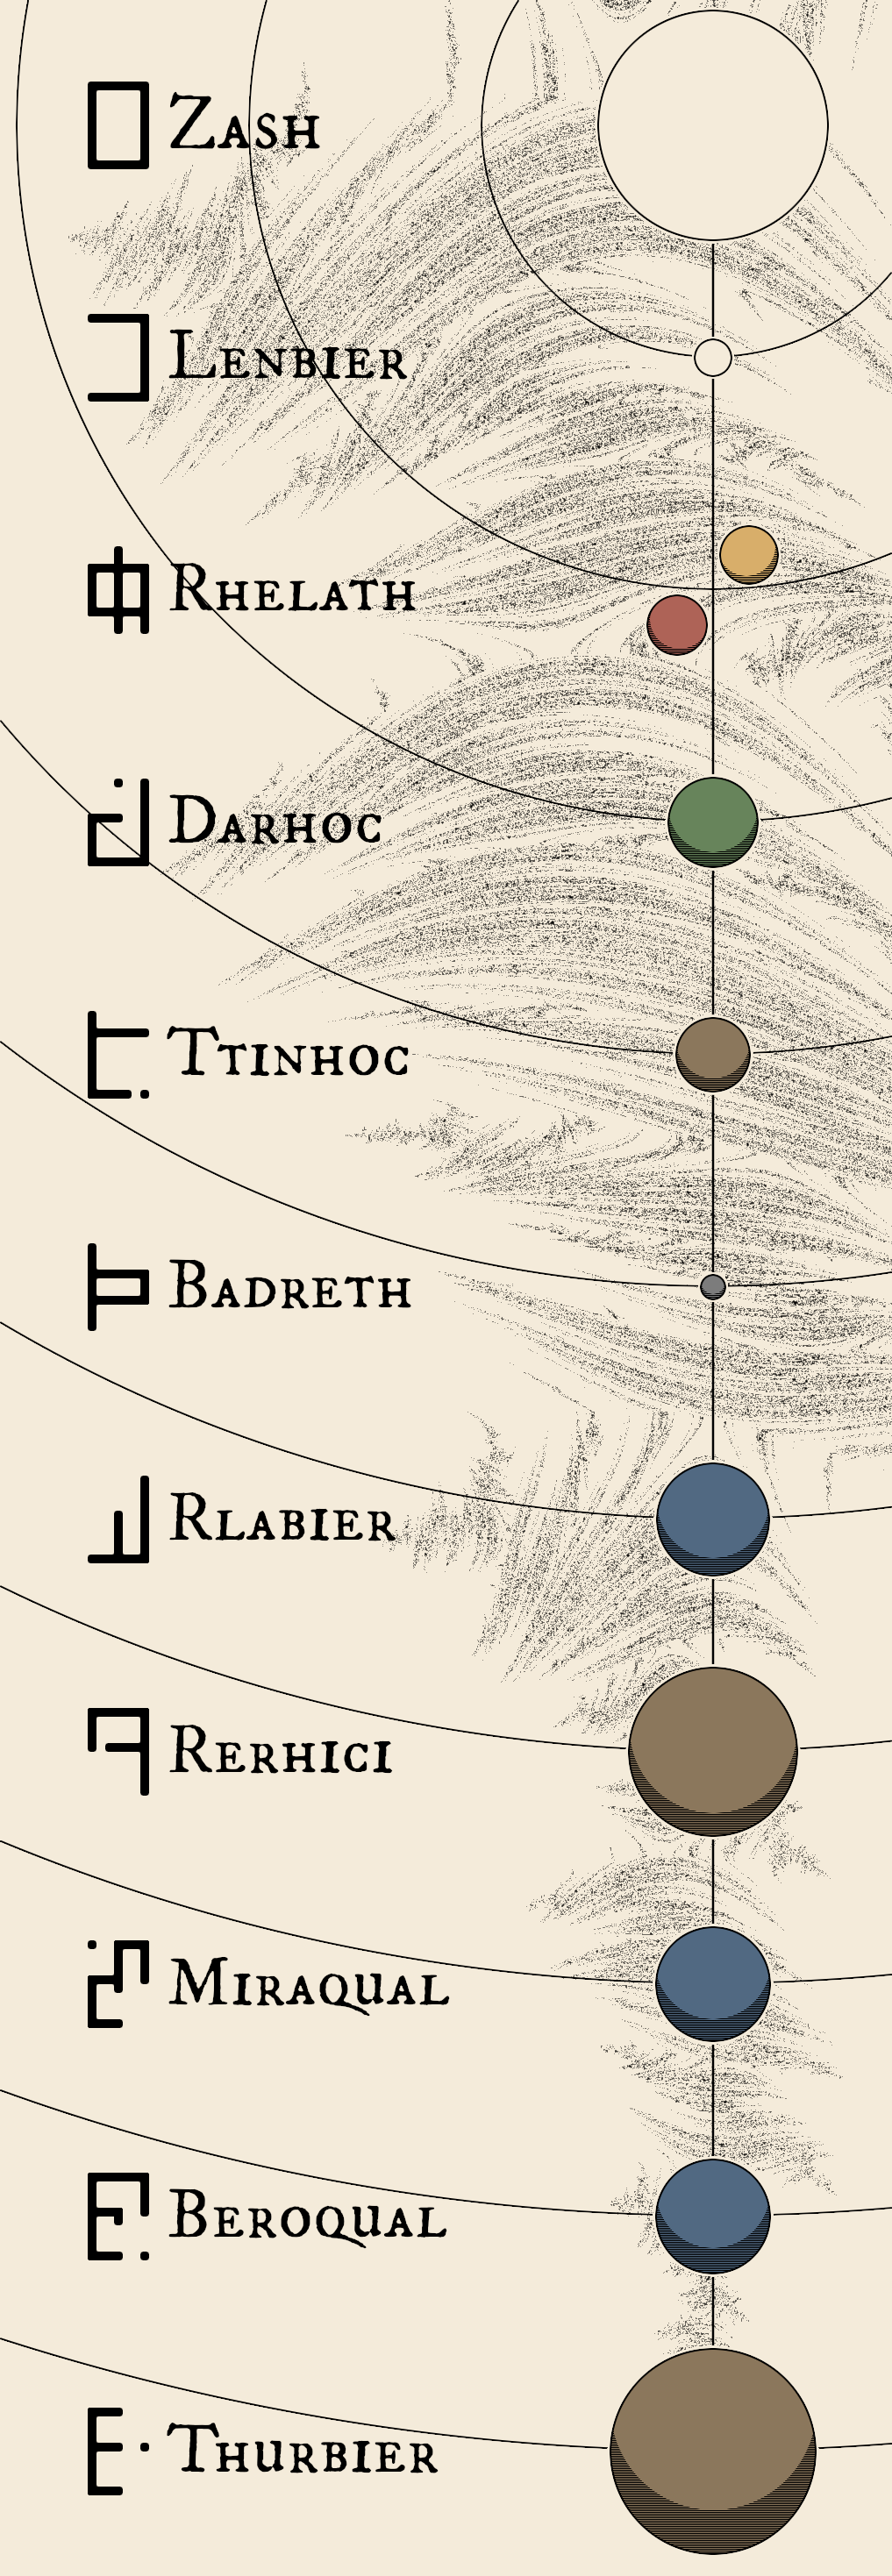
\includegraphics{01yuadrem/img/41solarsystem.png}
% \end{figure}

\section{Outer Planes}
Historically, the perception of the heavens in Yuadrem was inherited from the ets to the original oth scholars.
Despite this early rationalization, most religions still associated the heavens to divine beings or objects of mystical wonder.

% !TEX root = ../main.tex
\subsection*{Cosmology}

\newpage

% !TEX root = ../main.tex
\subsection*{The Five Moons}

\begin{table*}[b]%
    \begin{DndTable}[width=\linewidth]{X}
        \centering
        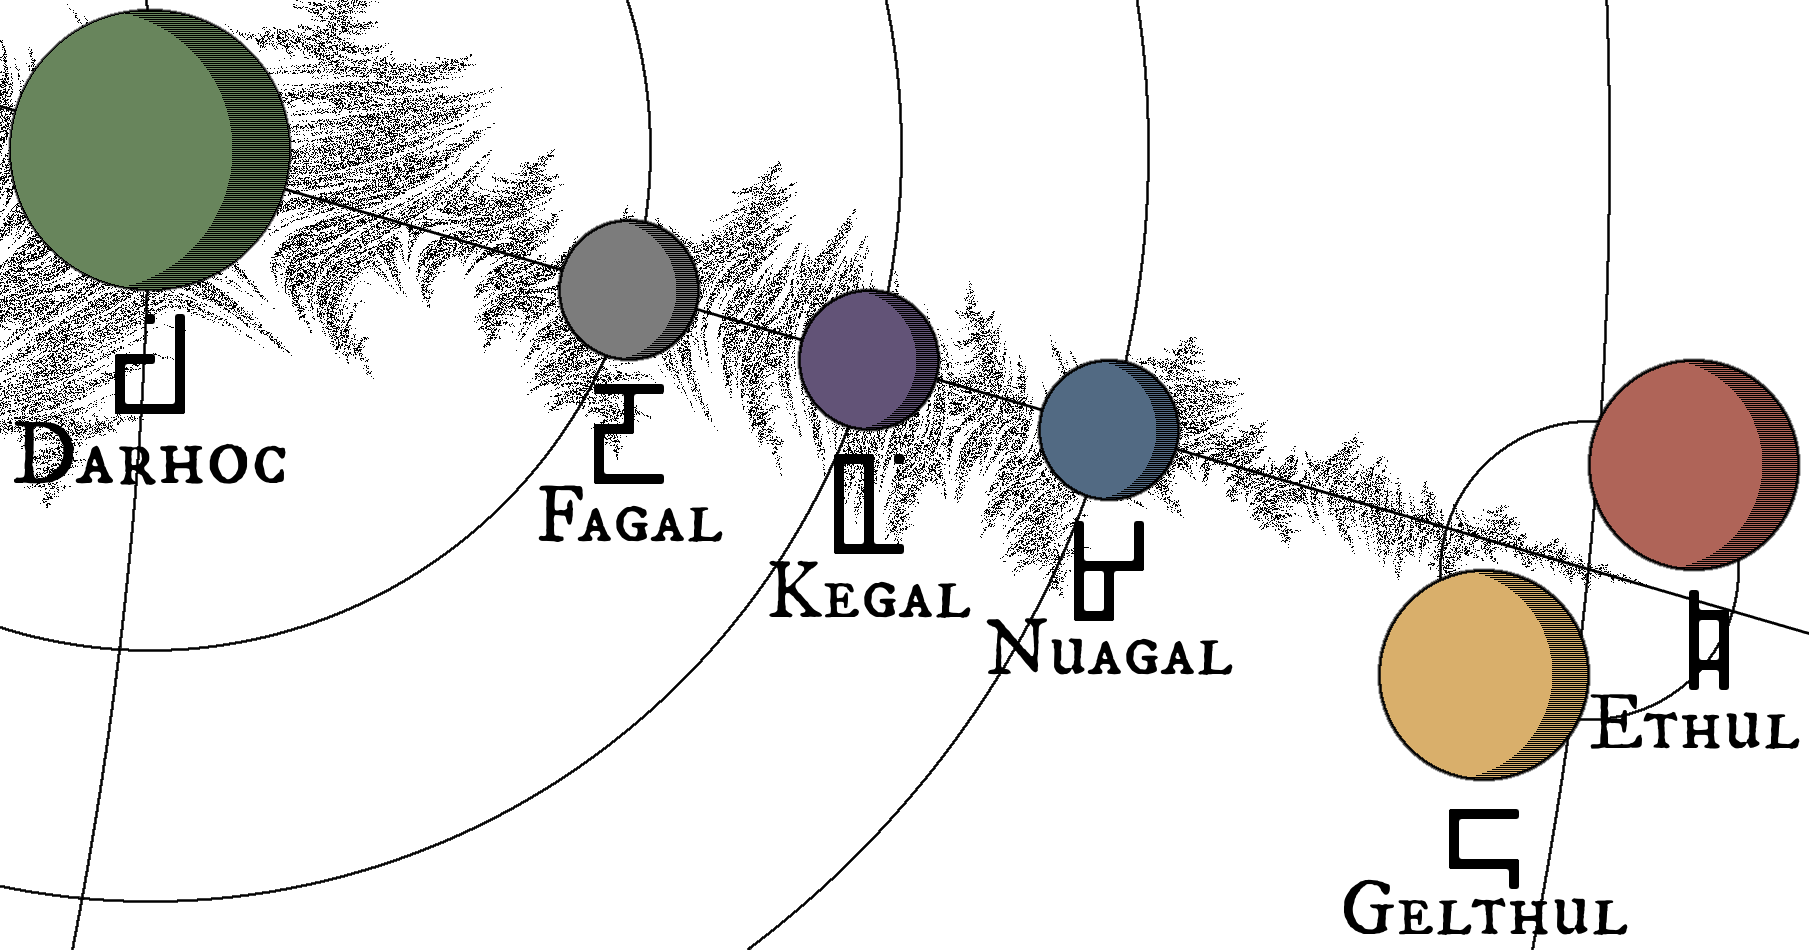
\includegraphics[width=0.99\textwidth]{01yuadrem/img/42moons.png}
    \end{DndTable}
\end{table*}

It is an undeniable fact of nature that moons have a strong effect over the tides.
In Yuadrem, this effect acts both on the ocean's tides and on the inviolate tides of the sentient mind.
Any religion or theory that attempts to explain the tides has to take the moons into consideration, for the two are intrinsecally linked.

The presence of three moons has interesting effects on the ocean tides.
Additionally, the ocassional influence of the twin planets of Rhelath adds more chaos to the system.
For centuries the tides were thought to be unpredictable, as impulsive and erratic as the whims of the mind.

This was until the then unknown oths of Abipolash designed the Nuagalian calendar.
Setting a year to two full translations of Nuagal, it predicts with astonishing accuracy the ocean's tides.
The ability to predict the tides enabled sailors to minimize risk in their journeys.
Some claim that only thanks to this calendar has the Whaler's Sea become the hub of commerce it is today.

There are some who claim to have visited the moons, supposedly through roads paved by the ets of yore.
While there is no substantial evidence to any of these claims, the vivid tales told by these explorers have left many to wonder.

While technically Yuadrem has three moons, the influence of the twin planets of Rhelath over the tides has made history count them as two additional moons.
A list of the moons along with a short description of each is provided.

\pagebreak

\subparagraph{Fagal} The largest and brightest object of the night sky, it is clear that Fagal seeks to be known by all people.
The patron moon of the Silver Tide, Fagal has the strongest influence over Yuadrem's tides, the water rising to kiss its gleaming face.
Its translation period is of 24 days, and its new moon marks the beginning of each month in the Fagalian calendar --- the most common calendar in Yuadrem.

\subparagraph{Kegal} Taking its place behind Fagal, Kegal takes its time to orbit Darhoc, observing even the loneliest commoner.
The patron moon of the Magenta Tide, Kegal's ever watchful eye is always attentive --- and judging --- of mortal lives.
Its translation period is of 48 days, and it is tidally locked to Yuadrem.

\subparagraph{Nuagal} The last of Darhoc's natural moons, Nuagal seems to mind its own business.
Intronspective and absorved, the patron moon of the Blue Tide holds no concern over mortal toil.
Its translation period is of 72 days, rotating freely and independant of Darhoc.

\subparagraph{Rhelath} The patron moons of the Gold and Red Tides respectively, Gelthul and Ethul are two planets locked in an eternal --- and deadly --- dance.
Some say that this dance represents the fiery fight inside oneself, the pull towards helping yourself against helping others.
% Roughly completing an orbit around each other twice a day, each moment that passes these two giants come closer to their eventual crash.

Gelthul and Ethul have orbitted each other for as long as sentience has existed in Yuadrem.%, and all predictions point to this continuing for the countless millenia to come.
The twin planets complete an orbit around Zash every 115 days, and approaches Darhoc every \textbf{TODO} years, wrecking havoc during their visit.

\pagebreak

% !TEX root = ../main.tex
\begin{tikzpicture}[remember picture,overlay]
    \node[anchor=north, yshift=0.10cm] at (current page.north) {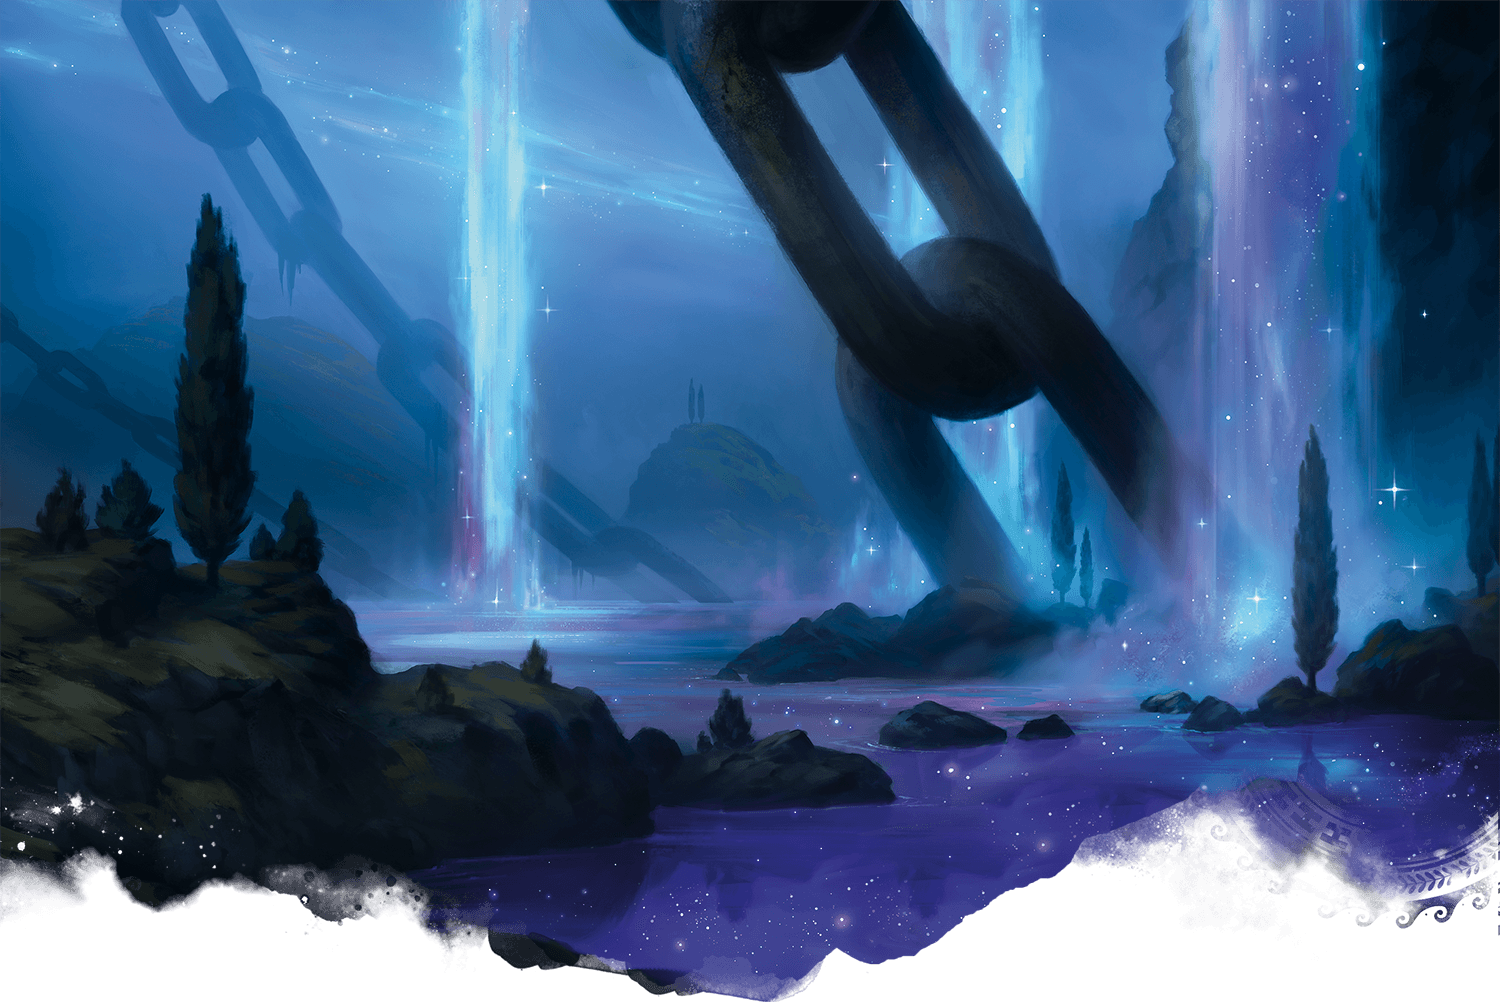
\includegraphics[width=\pdfpagewidth]{01yuadrem/img/43nyx.png}};
\end{tikzpicture}

\vspace{12.0cm}

\subsection*{Nyx}
% \DndDropCapLine{I}{f ever you find yourself beaten and}
% broke.
% And can't feel the wind for the weight of the yoke.
% And fear that the night will not turn into day.
% Remember the darkness will show you the way.
The Schism marked the beginning of an era, and with it came the opening of the Sizzling Gate.
% Through this gate spewed forth the foreigner kins, tortles, grungs, and umans.
On the other side of the portal is a strange realm, thought to be even farther from Darhoc than Thurbier.
Some even claim that this land is not even a planet at all, but an incarnation of the Cosmos itself.
This strange plane is known only as Nyx.

Nyx's topography is similar to that of Yuadrem's, its landscapes characterized by mountains, plains, ridges, etc.
Vast oceans of stars characterize the plane, fed by everflowing waterfalls of nebula.
Thick forests and fields of dark flora cover the shores, grazed by alien creatures known as the Nyxborn.

Titanic ruins and great, algae-slick chains rise out of the sea, as do the weathered remains of forgotten civilizations.
The sky is a misty blur of color that hangs over water as still as glass.
Mighty storms often arise from nowhere, casting souls into waves and whirlpools by the scores.

On especially dark new moons and eclypses, Nyx shows itself in the night sky, its ever-changing brilliance marked by consetellations and cosmic phenomena.
Some claim that during these nights the souls of the recently dead join their anscestors in this strange land.

\pagebreak~
\vspace{13.0cm}

While Nyx is impossible to map, distinct regions do exist, and some travelers have returned to the mortal realm with tales of these incredible locations.
Each of these regions is known as a ward, and is vast beyond understanding.
Most imagine these wards as being stacked atop one another, but their actual relationships defy mortal understanding.

\subsubsection{The Tartyx River}
There is one location however that all who have travelled to Nyx claim to have seen: The Tartyx River.
The Tartyx is vast, with one far shore impossible to see from the other.
Known as the Rivers That Ring the World, it is formed from the confluence of countless tributaries from unnumbered realms.

Countless drifting islands dot the river, some forested by leafless trees, others heaped with crumpling ruins.
Still others are the domains of strange entities that death proves not quite able to claim.
None of these tiny lands are hospitable to either the living or the dead.
The waters of the Tartyx hold their own threats, both mysterious creatures that slither beneath its rippling waters, and their own infamous power to wash away memories and all sense of identity.



    % !TEX root = ../main.tex
\chapter{Viphoger} \label{ch::viphoger}
\DndDropCapLine{A}{s a new nation, Viphoger is small. Its}
poleis are minuscule in comparison to the wilderness beyond, but their inhabitants live joyfully in their newly earned independence.

\begin{table*}[b]
\begin{DndTable}[width=\linewidth, header=Fagalian Calendar]{cXXX}
    \textbf{Month} & \textbf{Name} & \textbf{Tide} & \textbf{God} \\
    1              & Amion         & Blue          & Heliod, God of the Sun \\
    2              & Sianion       & Gold          & Ephara, God of the Polis \\
    3              & Granion       & Magenta       & Iroas, God of Victory \\
    4              & Zmivion       & Silver        & Phenax, God of Deception \\
    5              & Skenion       & Red           & Mogis, God of Slaughter \\
    6              & Danion        & Blue          & Kruphix, God of Horizons \\
    7              & Dibinion      & Gold          & Purphoros, God of the Forge \\
    8              & Ranion        & Magenta       & Athreos, God of Passage \\
    9              & Amelamion     & Silver        & Thassa, God of the Sea \\
    10             & Amelsion      & Red           & Erebos, God of the Dead \\
    11             & Amelgranion   & Blue          & Pharika, God of Affliction \\
    12             & Amelzvion     & Gold          & Nylea, God of the Hunt \\
    13             & Amelskenion   & Magenta       & Klothys, God of Destiny \\
    14             & Ameldanion    & Silver        & Karametra, God of Harvests \\
    15             & Ameldibinion  & Red           & Keranos, God of Storms \\
    16*            & Fisimmas      & White         & The Sorrow
\end{DndTable}
\end{table*}
% * This day only occurs once every ten years.

Viphoger consists of a peninsula forming the south-western edge of the vast Whaler's Sea.
South from the sea, the land rises up to a ridge of mountains.
The lofty peaks of this ridge forms a barrier that few cross, so only rumors of the vast Dead Sea describe the land beyond.

To the west, the coastal lands become small pockets of forests crossed by a labyrinth of arid canyons, with the Zoedrem desert beyond.

The Siren's inlet to the north is studded with islands large and small.
The largest cluster near the mainland, called the Dakra Isles, is poorly charted, and even those sailors who attempt to explore the isles return with contradictory information.
Eastward from Viphoger, the old nations of Yuadrem trade in the Whaler's Sea. % , regulated by the strong influence of the Seven Kingdoms of the Sea.

The heart of Viphoger lies in and around three poleis—cities and their surrounding territories.
Together the three poleis, Akhosh, Mephetis, and Setesh, encompass most of the population of Viphoger.
Mephetis covers the whole territory of the northeastern peninsula, Akhosh forms the frontier to the desert, and Setesh lies at the northern edge of the wild Nessian Wood.

The bands of the Uqhardu, the Vahagha, and the Pheres, roam the hills and badlands between the three poleis.
Remnants of the once great empire of Hulnar, now reduced to bandits and traders.
The mysterious leonin hunt in the valley of Oreskos, nestled between Mt. Kure and Winter's Heart.
Bughna gats and marsets dwell around the Stola Vale and the larger Nessian Wood.
And tortles live primarily in the coastal shallows of the Siren Inlet, though some manage to make comfortable homes among the gats of Mephetis.

The canyon of Katajthon, south of Akhosh, is the frontier where Akhoshian soldiers clash with Treb gats.
Farther south-west is the city of Kofos, little known to Viphogerians.

The necropoleis of Asphodel and Odunos are home to the Returned --- zombie-like beings who have contracted the Illness.
Access to these lands is strictly forbidden, and is punishable by death in all three poleis.
The lands around these cities are bleak and barren, as if the Returned brought the pall of the underworld out with them into the mortal realm.

% !TEX root = ../main.tex
\subsection*{The Fagalian Calendar} \label{ssec::thefagaliancalendar}
The oth astronomers and philosophers from oldentimes established a calendar that has found massive adoption in the rest of Yuadrem.
It divides the year into fifteen months of twenty-four days, each beginning after the new Fagal.
Every ten years, an extra day is added at the end of the calendar to keep it aligned with the solar year.

The beginning of the year is considered the end of spring, so the new year begins with the summer.
Each month is associated to a tide, and is holy to a specific god.
A major festival in honor of that god is celebrated in Mephetis.
The fifth month (Skenion in Mephetis) is called Iroagonion in Akhosh, after the Iroan Games, which are held in that month every year.

% The Fagalian Calendar table summarizes the months, their lengths, and the god each is associated with.

% !TEX root = ../main.tex
\subsection*{Life in the Poleis} \label{ssec::lifeinthepoleis}
Civilization in Viphoger is centered in three poleis: Akhosh, Mephetis, and Setesh.
These poleis exemplify the kins' drive to settle the land, to shape nature according to their needs, and to organize into political structures that can withstand the changing fortunes of the passing centuries.

Each polis is centered in a city but includes a wide region of surrounding territory, and each one has its own distinct society and culture.
To the people of Viphoger, ``Mephetis'' is more or less synonymous with ``Mephetians'' --- the polis isn't just the people who live in the city of Mephetis or even those who dwell in nearby villages; it is the people who follow the Mephetian way of life, wherever they might be found.

\subsubsection{Citizenship and Government}
In every polis, civic responsibility and full protection are afforded only to citizens.
Citizenship is limited to those whose parents were both citizens of the polis.
Citizens of other poleis, and their children, aren't permitted to participate in the government of the polis.
In Akhosh, citizens must meet one additional requirement: they must serve in the army.

The three poleis have different political structures, but each one has a council elected by popular vote of the citizenry.
The Twelve, Mephetis's council of philosophers, is the democratically elected ruling body of the polis.
Akhosh is ruled by a hereditary monarch who is advised by a council of elders elected by and from among the citizenry.
Similarly, Setesh's Ruling Council is formed by popular vote, and they govern the polis while its queen --- the goddess Karametra --- is absent.

\subsubsection{Trade and Currency}
Trade between Akhosh and Mephetis is constant and productive.
Caravans make the two-week journey between the poleis twice a month, aided by the Tsher river.
They carry fine Akhoshian metalwork and pottery to Mephetis, and Mephetian fabric, stonework, and fish westward.
Both poleis mint coins of copper, silver, and gold, with equivalent value.

Setesh trades with the other poleis as well, but less extensively.
Its Abora Market, just inside the city gates, is open to outsiders only on certain days, and Seteshan merchants prefer to barter goods rather than accept currency.
Despite these restrictions, Seteshan food, woodwork, and trained falcons are highly valued in the other poleis.

Aside from the other poleis, Mephetis and Setesh both trade with the dratl irds of the Vahagha band.
The irds don't work metal, so they trade woodwork, the produce of the plains, and woven blankets to the human poleis in exchange for weapons and armor.

\subsubsection{Recreation}
The people of the poleis enjoy the opportunity for some recreation, as time and money allow.

Gymnasia are popular gathering places, offering athletic training as well as space for philosophical discussion and friendly socializing.
A resident of the city might visit a gymnasium one day to exercise, the next to view a wrestling match between celebrated competitors, and the next to hear a renowned philosopher give a lecture on ethics.

Another important venue for recreation is the theater.
The works of celebrated playwrights, past and present, are regularly produced by casts of professional actors.
On occasion, a storyteller, accompanied by a small orchestra, draws crowds to a theater for a recitation of one of the great epics, such as The Sylvan Wars, The Theriad, or The Callapheia.
Such a performance might stretch over two or three days.


\incgraph[documentpaper,][width=\paperwidth,height=\paperheight]{02viphoger/img/00map.png}
\newpage~

    \DndSetThemeColor[DmgCoral]
    % !TEX root = ../main.tex
\chapter{Mechanic Changes} \label{ch::mechanicchanges}

\DndDropCapLine{S}{trands may break alone, but twisted}
\textit{make a braid.
Together on their own, the journey shall be made.}

\hspace*{\fill} --- Anonymous song.

This book includes major mechanical changes.
These mostly focus on allowing players to embrace the worldbuilding aspects of Yuadrem by freeing up their character building options.
These changes are of course optional, but most of the rules in the book were designed with them in mind.

Then, optional rules are included.
Yuadrem is a harsh continent, and these rules help set the atmosphere to reflect this.
They are completely optional, and a healthy gaming table should discuss which should be included or excluded in their game.

\begin{DndComment}[float=h]{Help Wanted!}
    This entire book was designed with the major mechanical changes considered, yet the author realizes that this can alienate a large part of the community.
    You may want to play in Yuadrem without these changes.
    If this is the case, many other mechanics need to be changed accordingly to acommodate this.

    If for some insane reason you want to take on this challenge, you are encouraged to contact the book's author.
    We could work together on this, discussing appropiate retribution and co-authorship terms.
\end{DndComment}

% !TEX root = ../main.tex
\section{3-Action System} \label{sec::3actionsystem}
Instead of the movement, action, and bonus action system of D\&D 5e, this book uses Pathfinder 2e's 3-action system.
Simply put, you can use up to three Action Points (AP) in a turn.
Additionally, one free action and one reaction per round are available.

The number of AP used by an action is denoted by the $\circ$ symbol.
Reactions are denoted by the $\otimes$ symbol.

The standard actions and reactions available to you are:

\subsubsection{Attack $\circ$} \label{act::attack}
    \textit{Perform a melee or ranged attack with your weapon.}

    You can use more than one Attack action on your turn, but each additional attack after the first becomes less accurate.
    This is reflected by a multiple attack penalty that starts at -5 on the second attack, increases to -10 on the third, -15 on the fourth, etc.
    This penalty resets at the end of your turn.

    Some conditions give advantage on the attack: attacks against blinded, paralyzed, petrified, restrained, stunned, or unconscious targets; melee attacks against prone targets; attacks by invisible or hidden attackers.

    Some conditions give disadvantage on the attack: attacks against invisible or hidden targets; ranged attacks against prone targets; attacks by blinded, frightened, poisoned, or restrained attackers.
\subsubsection{Cast a Spell $\ast$} \label{act::castaspell}
    \textit{Cast a spell with a casting time of 1 or more actions.}

    The target of a spell must be within the spell's range.
    To target something, you must have a clear path to it, so it can't be behind total cover.

    Spells with material components do not consume the material unless explicitly stated.
    Unless the cost of a material is given, you can assume that the cost is negligible and the material is simply available in a component pouch.

    Some spells require you to maintain concentration in order to keep their magic active.
    If you lose concentration, such a spell ends.
    You lose concentration on a spell if you cast another spell that requires concentration or when you are incapacitated.
    Each time you take damage, you must make a Constitution saving throw to maintain your concentration.
    The DC equals 10 or half the damage you take, whichever number is higher.
\subsubsection{Climb onto a Bigger Creature $\circ\circ$}  \label{act::climbontoabiggercreature}
    \textit{Hop atop your target.}

    You can treat a suitably large opponent as terrain for the purpose of jumping onto its back or clinging to a limb.
    After making any ability checks necessary to get into position and onto the larger creature, you use an action to make a Strength (Athletics) or Dexterity (Acrobatics) check contested by the target's Dexterity (Acrobatics) check.
    If you win the contest, you successfully move into the target creature's space.
    You move with the target and have advantage on attack rolls against it.

    You can move around within the larger creature's space, treating it as difficult terrain.
    The larger creature's ability to attack you depends on your location, and is left to the DMs discretion.
    The larger creature can dislodge you as an action—knocking you off, scraping you against a wall, or grabbing and throwing you—by making a Strength (Athletics) check contested by the your Strength (Athletics) or Dexterity (Acrobatics) check.
    You choose which ability to use.

\pagebreak

\subsubsection{Disarm $\circ\circ$} \label{act::disarm}
    \textit{Force your opponent to unequip their weapon.}

    You can use an action to knock a weapon or another item from a target's grasp.
    You make an attack roll contested by the target's Strength (Athletics) check or Dexterity (Acrobatics) check.
    If you win the contest, the attack causes no damage or other ill effect, but the defender drops the item.

    You have disadvantage on the attack roll if your target is holding the item with two or more hands.
    The target has advantage on its ability check if it is larger than you, or disadvantage if it is smaller.
\subsubsection{Disengage $\circ\circ$} \label{act::disengage}
    \textit{Your movement doesn't provoke opportunity attacks for the rest of the turn.}
\subsubsection{Dodge $\circ\circ$} \label{act::dodge}
    \textit{Focus entirely on avoiding attacks.}

    Until the start of your next turn, any attack roll made against you has disadvantage if you can see the attacker, and you make Dexterity saving throws with advantage.

    You lose this benefit if you are incapacitated or if your speed drops to 0.
\subsubsection{Equip Shield $\circ\circ$} \label{act::equipshield}
    \textit{Equip or unequip a shield.}

    A shield takes two actions to equip or unequip.

    Armor takes several minutes to equip or unequip.
\subsubsection{Escape $\circ$} \label{act::escape}
    \textit{Escape a grapple.}

    To escape a grapple, you must succeed on a Strength (Athletics) or Dexterity (Acrobatics) check contested by the grappler's Strength (Athletics) check.

    Escaping other conditions that restrain you (such as manacles) may require a Dexterity or Strength check, as specified by the condition.
\subsubsection{Grapple $\circ$} \label{act::grapple}
    \textit{Attempt to grab a creature or wrestle with it.}

    The target of your grapple must be no more than one size larger than you, and it must be within your reach.

    Using at least one free hand, you try to seize the target by making a grapple check, a Strength (Athletics) check contested by the target's Strength (Athletics) or Dexterity (Acrobatics) check (the target chooses the ability to use).

    If you succeed, you subject the target to the grappled condition (its speed is set to 0).
\subsubsection{Help $\circ$} \label{act::help}
    \textit{Grant an ally within 1 meter advantage on an ability check or attack.}

    The target gains advantage on the next ability check it makes to perform the task you are helping with.
    Alternatively, the target gains advantage on the next attack roll against against a creature within 1 meter of you.

    The advantage lasts until the start of your next turn, and you can use this action only once per turn.
\subsubsection{Hide $\circ\circ$} \label{act::hide}
    \textit{Attempt to hide.}

    You can't hide from a creature that can see you.
    You must have total cover, be in a heavily obscured area, be invisible, or otherwise block the enemy's vision.

    If you make noise (such as shouting a warning or knocking over a vase), you give away your position.

    When you try to hide, make a Dexterity (Stealth) check and note the result.
    Until you are discovered or you stop hiding, that check's total is contested by the Wisdom (Perception) check of any creature that actively searches for signs of your presence.

    A creature notices you even if it isn't searching unless your Stealth check is higher than its Passive Perception.

    Out of combat, you may also use a Dexterity (Stealth) check for acts like concealing yourself from enemies, slinking past guards, slipping away without being noticed, or sneaking up on someone without being seen or heard.
\subsubsection{Identify a Spell $\circ/\otimes$} \label{act::identifyaspell}
    \textit{Attempt to understand a cast spell.}

    Sometimes you may want to identify a spell that someone else is casting or that was already cast.
    To do so, you can use your reaction to identify a spell as it's being cast, or use an action on your turn to identify a spell by its effect after it is cast.

    If you perceived the casting, the spell's effect, or both, you can make an Intelligence (Arcana) check with the reaction or action.
    The DC equals 10 + the spell's level.
    If the spell cast is from a school of magic in which you have competence, the check is made with advantage.
    Some spells aren't associated with any school, such as when a monster uses its Innate Spellcasting trait.

    This Intelligence (Arcana) check represents the fact that identifying a spell requires a quick mind and familiarity with the theory and practice of casting.
    This is true even for a character whose spellcasting ability is Wisdom or Charisma.
    Being able to cast spells doesn't by itself make you adept at deducing exactly what others are doing when they cast their spells.
\subsubsection{Improvise $\circ$} \label{act::improvise}
    \textit{Perform any action you can imagine.}

    When you describe an action not detailed elsewhere in the rules, the DM tells you whether that action is possible and what kind of roll you need to make, if any, to determine success or failure.
\subsubsection{Move $\circ$} \label{act::move}
    \textit{Move up to your movement speed.}

    You can interrupt the move action to take another action, continuing your move afterwards.

    If you have more than one speed, such as your walking speed and a flying speed, you can switch back and forth between your speeds during your move.
    Whenever you switch, subtract the distance you've already moved from the new speed.

    You can move through a nonhostile creature's space.
    You can move through a hostile creature's space only if the creature is at least two sizes larger or smaller than you.
    Another creature's space is difficult terrain for you.
    Whether a creature is a friend or an enemy, you can't willingly end your move in its space.

    Climbing, swimming, and crawling cost an additional 1 m per 1 m traveled, unless you have an specific climbing or swimming speed.

    This movement can include a high jump and/or a long jump, following the normal rules for each.
\subsubsection{Overrun $\circ$} \label{act::overrun}
    \textit{Force your way through a creature's space.}

    When you try to move through a hostile creature's space, you try to force your way through by overrunning the hostile creature.
    As an action, you make a Strength (Athletics) check contested by the hostile creature's Strength (Athletics) check.
    You have advantage on this check if you are larger than the hostile creature, or disadvantage if you are smaller.
    If you win the contest, you can move through the hostile creature's space once this turn.
\subsubsection{Ready $\ast$} \label{act::ready}
    \textit{Choose a trigger and a response reaction.}

    First, you decide what perceivable circumstance will trigger your reaction.

    Then, you choose the action you will take in response to that trigger, or you choose to move up to your speed in response to it.

    When the trigger occurs, you can either take your reaction right after the trigger finishes or ignore the trigger.

    When you ready a spell, you cast it as normal but hold its energy, which you release with your reaction when the trigger occurs.
    Holding onto the spell's magic requires concentration.

    The cost of this action is equal to the cost of the readied action, so 1 for the attack action, 2 for the Search action, etc.
\subsubsection{Reload $\circ$} \label{act::reload}
    \textit{Reload a crossbow or firearm.}

    Some weapons require more than one action to reload.
    This is specified in the weapon itself.
\subsubsection{Search $\circ\circ$} \label{act::search}
    \textit{Devote your attention to finding something.}

    Depending on the nature of your search, the DM might have you make a Wisdom (Perception) check or an Intelligence (Investigation) check.
\subsubsection{Shove $\circ$} \label{act::shove}
    \textit{Shove a creature, either to knock it prone or push it to the side.}

    The target of your shove must be no more than one size larger than you, and it must be within your reach.

    You make a Strength (Athletics) check contested by the target's Strength (Athletics) or Dexterity (Acrobatics) check (the target chooses the ability to use).

    If you win the contest, you either knock the target prone or push it 1 meter to the side (your choice).
\subsubsection{Stabilize a Creature $\circ\circ$} \label{act::stabilizeacreature}
    \textit{Stop a dying creature from needing to make death saving throws.}

    Make a Wisdom (Medicine) check with DC 10.

    On a success, the creature is stable and no longer needs to make death saving throws.

    A stable creature regains 1 hit point after 1d4 hours.
\subsubsection{Stand Up $\circ$} \label{act::standup}
    \textit{End the prone condition on yourself by standing up.}
\subsubsection{Tumble $\circ$} \label{act::tumble}
    \textit{Weave past a hostile creature.}

    You can try to tumble through a hostile creature's space, ducking and weaving past the opponent.
    As an action, you make a Dexterity (Acrobatics) check contested by the hostile creature's Dexterity (Acrobatics) check.
    If you win the contest, you can move through the hostile creature's space once this turn.
\subsubsection{Use Object $\circ\circ$} \label{act::useobject}
    \textit{Interact with a second object or use special object abilities.}

    You can interact with one object for free during your turn (such as drawing a weapon or opening a door).
    If you want to interact with a second object, use this action.

    When an object requires your action for its use, you also take this action.
\subsubsection{Cast a Spell $\otimes$} \label{act::castaspellreact}
    \textit{Cast a spell with a casting time of 1 reaction.}

    Trigger: specified by the spell.

    For further details, see the Cast a spell action.
\subsubsection{Readied Action $\otimes$} \label{act::readiedaction}
    \textit{Execute the reaction specified by your Ready action.}

    Trigger: specified by your Ready action.
\subsubsection{Opportunity Attack $\otimes$} \label{act::opportunityattack}
    \textit{You can rarely move heedlessly past your foes without putting yourself in danger.}

    Trigger: enemy creature leaves your reach.

    Make one melee attack against the provoking creature.

    The attack interrupts the provoking creature's movement, occurring right before the creature leaves your reach.

    Creatures don't provoke an opportunity attack when they teleport or when someone or something moves them without using their movement, action, or reaction.

    Additional conditions for opportunity attacks are included as an optional rule in page \pageref{rule::opportunityattacks}.

\subsection*{Learnable Actions} \label{ssec::learnableableactions}
    Some actions are not available by default, but instead require learning a feat to be obtained.
    These are listed in this subsection, along with links to the feats required to learn them.
    The \textbf{Adaptable Fighter} (page \pageref{feat::adaptablefighter}) and \textbf{Dynamic Fighter} (page \pageref{feat::dynamicfighter}) feats allow you to learn an action of your choice.

    \subsubsection{Aim $\circ$} \label{act::aim}
        You give yourself advantage on your next attack roll, which can be made until the end of your next turn.

        This action can be obtained from the \textbf{Deadly Precision} (page \pageref{feat::deadlyprecision}) and the \textbf{Eye for Weakness} (page \pageref{feat::eyeforweakness}) feats.
    \subsubsection{Block $\otimes$} \label{act::block}
        You can use your reaction to prepare yourself against one melee or ranged attack.
        You increase your AC by 1d6 against the attack.
        If the attack does hit you, you take half damage from it (rounded down).

        This reaction can be obtained from the \textbf{Stalwart Stance} feat (page \pageref{feat::stalwartstance}).
    \subsubsection{Distracting Strike $\circ\circ$} \label{act::distractingstrike}
        You use your action to distract a creature with an attack, giving your allies an opening.
        You roll damage normally, and the next attack roll against the target by an creature other than you has advantage if the attack is made before the start of your next turn.

        This action can be obtained from the \textbf{Flourished Duelist} (page \pageref{feat::flourishedduelist}) feat.
    \subsubsection{Quick Draw $\otimes$} \label{act::quickdraw}
        You can make an attack of opportunity with an equipped thrown or ranged weapon when a creature moves out of a 9-meter radius around you.

        This reaction can be obtained from the \textbf{Quick Draw} (page \pageref{feat::quickdraw}) and the \textbf{Quick Shot} (page \pageref{feat::quickshot}) feats.
    \subsubsection{Mark $\circ\circ$} \label{act::mark}
        You choose a creature you can see within 18 meters and mark it as your quarry.
        For up to one hour, you deal an extra 1d6 damage to the target whenever you hit it with a weapon attack, and you have advantage on any Intelligence (Investigation), Wisdom (Perception), and Wisdom (Survival) checks you make to find it.
        You can use this action a number of times equal to your Wisdom modifier, and you restore all expended uses on a short rest.

        This action can be obtained from the \textbf{Tracker} (page \pageref{feat::tracker}) and the \textbf{Mark} (page \pageref{feat::mark}) feats.
    \subsubsection{Parry $\otimes$} \label{act::parry}
        When another creature attacks you with a melee attack, you can use your reaction to increase your AC by 1d6 + your Dexterity modifier against the attack.

        This reaction can be obtained from the \textbf{Parrying Stance} (page \pageref{feat::parryingstance}), the \textbf{Swift Deflection} (page \pageref{feat::swiftdeflection}), and the \textbf{Sword Breaker} (page \pageref{feat::swordbreaker}) feats.
    \subsubsection{Push $\circ$} \label{act::push}
        You try to push a target back.
        The target must be no more than one size larger than you and be within 1 meter of you.
        You make a Strength (Athletics) check contested by the target's Strength (Athletics) or Dexterity (Acrobatics) check (the target chooses the ability to use).
        If you win, you push the target up to 3 meters away from you.
        If you win by 10 or more, the target is also knocked prone.

        This action can be obtained from the \textbf{Forest Defender} (page \pageref{feat::forestdefender}) and \textbf{Stalwart Shield} (page \pageref{feat::stalwartshield}) feats.
    \subsubsection{Reckless Attack $\circ$} \label{act::recklessattack}
        You make a special melee weapon attack against a creature using a weapon with the heavy property.
        Apply a -5 penalty to the attack roll.
        If the attack hits, you add +10 to the attack's damage.

        This action can be obtained from the \textbf{Giant Slayer} (page \pageref{feat::giantslayer}), the \textbf{Heavy Hitter} (page \pageref{feat::heavyhitter}), and the \textbf{Reckless Attack} (page \pageref{feat::recklessattack}) feats.
    \subsubsection{Reckless Shot $\circ$} \label{act::recklessshot}
        You make a special ranged weapon attack against a creature with a ranged weapon.
        Apply a -5 penalty to the attack roll.
        If the attack hits, you add +10 to the attack's damage.

        This action can be obtained from the \textbf{Reckless Shot} (page \pageref{feat::recklessshot}) feat.
    \subsubsection{Riposte $\otimes$} \label{act::riposte}
        When a creature misses you with a melee attack, you can use your reaction to make a melee weapon attack against the creature.

        This action can be obtained from the \textbf{Appropiate Response} (page \pageref{feat::appropiateresponse}) feat.
    \subsubsection{Sneak Attack $\circ\circ$} \label{act::sneakattack}
        You know how to strike subtly and exploit a foe's distraction.
        You do an attack that deal an extra 2d6 damage to one creature you hit with an attack if you have advantage on the attack roll.
        The attack must use a finesse or a ranged weapon.

        You don't need advantage on the attack roll if another enemy of the target is within 5 feet of it, that enemy isn't incapacitated, and you don't have disadvantage on the attack roll.
        You can use this action only once per turn.

        You can take this action various times.
        Each time after the first increases the number of d6s rolled by one.

        This action can be learned and improved from the \textbf{Hidden Striker} (page \pageref{feat::hiddenstriker}), the \textbf{Purposeful Strike} (page \pageref{feat::purposefulstrike}) and the \textbf{Stab-a-Lung} (page \pageref{feat::stabalung}) feats.
    \subsubsection{Steal $\circ\circ$} \label{act::steal}
        As an action, you can make a Dexterity (Sleight of Hand) check contested by a creature's Wisdom (Perception) to plant something on someone else, conceal an object on a creature, lift a purse, or take something from a pocket.
        You can do this in the middle of an encounter.

        This action can be learned from the \textbf{Poacher} (page \pageref{feat::poacher}) feat.
    % === UNUSED ============================================================ %
    % \subsubsection{Careless Deflect} \label{tec::carelessdeflect}
    %     When a creature misses you with a melee attack roll, you can use your reaction to cause that attack to hit one creature of your choice, other than the attacker, that you can see within 1 meter of you.
    %
    % \subsubsection{Commander's Strike} \label{tec::commandersstrike}
    %     When you take the Attack action on your turn, you can choose to attack only once and use a bonus action to direct one of your companions to strike.
    %     When you do so, choose a friendly creature who can see or hear you.
    %     That creature can immediately use its reaction to make one weapon attack, adding a d8 to the attack's damage roll.
    %
    % \subsubsection{Disarming Attack} \label{tec::disarmingattack}
    %     You use your action to attempt to disarm the target with an attack, forcing it to drop one item of your choice that it's holding.
    %     The target must make a Strength saving throw with a DC of 8 + your proficiency bonus + your Strength modifier.
    %     On a failed save, it drops the object you choose.
    %     The object lands at its feet.
    %
    % \subsubsection{Evasive Footwork} \label{tec::evasivefootwork}
    %     When you move, you can use a bonus action to add a d6 to your AC until you stop moving.
    %
    % \subsubsection{Goading Attack} \label{tec::goadingattack}
    %     You use your action to attack a creature and goad it into attacking you.
    %     The target must make a Wisdom saving throw with a DC of 8 + your proficiency bonus + your Charisma modifier.
    %     On a failed save, the target has disadvantage on all attack rolls against targets other than you until the end of your next turn.
    %
    % \subsubsection{Injure} \label{tec::injure}
    %     As an action, you can attack with the sole purpose of injuring a creature.
    %     Roll your weapon attack normally.
    %     On a hit, you deal only half damage, but the creature rolls on the minor injury chart.
    %     If the attack is a critical hit, the creature rolls on the major injury chart.
    %
    % \subsubsection{Maneuvering Attack} \label{tec::maneuveringattack}
    %     When you hit a creature with a melee attack, you can use your bonus action to maneuver one of your comrades into a more advantageous position.
    %     You choose a friendly creature who can see or hear you.
    %     That creature can use its reaction to move up to half its speed without provoking opportunity attacks from the target of your attack.
    %
    % \subsubsection{Menacing Attack} \label{tec::menacingattack}
    %     When you hit a creature with a weapon attack, you can use your bonus action to attempt to frighten the target.
    %     The target must make a Wisdom saving throw of a DC of 8 + your proficiency bonus + your Charisma modifier.
    %     On a failed save, it is frightened of you until the end of your next turn.
    %
    % \subsubsection{Precise Attack} \label{tec::preciseattack}
    %     When you make a weapon attack roll against a creature, you can use your bonus action to add a d8 to the attack roll.
    %     You can use this technique before or after making the attack roll, but before any effects of the attack are applied.
    %
    % \subsubsection{Rapid Repair} \label{tec::rapidrepair}
    %     You can attempt to repair a misfired (but not broken) firearm as a bonus action.
    %
    % \subsubsection{Violent Shot} \label{tec::violentshot}
    %     When you make a firearm attack against a creature, you can tune your weapon to enhance the volatility of the attack.
    %     The attack gains a +2 to the firearm's misfire score.
    %     If the attack hits, you can roll one additional weapon damage die.
    % \subsubsection{Predetermined Fate} \label{mtec::predeterminedfate}
    %     Whenever you make a saving throw and fail, you can reroll it and take the second result.
    %
    % \subsubsection{Quivering Palm} \label{mtec::quiveringpalm}
    %     This is the ultimate technique of the SCHOOL school, and can only be learned after you learn all other martial arts techniques.
    %     When you hit a creature with an unarmed strike, you can use the quivering palm technique.
    %     The creature must make a Constitution saving throw or take 10d10 bludgeoning damage, taking half damage on a success.
    %     You can use this technique only once per short rest.

\newpage~\newpage

% !TEX root = ../main.tex
\section{Classless D\&D} \label{sec::classlessdnd}

Due to the major differences in both style and setting between Yuadrem and other D\&D settings, most classes don't fit very well into it.
Instead of designing new classes, a classless system is introduced.
This system is inspired by many different, well-tested sources (Credits in addenda).

The details of this system are described in detail in its own chaper at page \pageref{ch::classlessdnd}.

% !TEX root = ../main.tex
\section{Feats}
For simplicity, feats are separated into six categories: feats related to kin, background, skills, proficiencies, combat, and spellcasting.
Each category is listed in the following pages.
Categories are ordered alfabetically, but each is listed in an easy to follow fashion in their respective sections.

Unless specified otherwise, a feat can only be learned once.

% !TEX root = ../main.tex
\addcontentsline{toc}{section}{Kin Feats}
\subsection*{Kin Feats}
\begin{DndTable}[width=\linewidth, header=Kin Feat List 1/3]{ll}
    \textbf{Kin or Subrace} & \textbf{Feat} \\
    Gat           & \textbf{Efficient Craftsgat} (page \pageref{feat::efficientcraftsgat})   \\
    Gat           & \textbf{Force of Will} (page \pageref{feat::forceofwill})                \\
    Gat           & \textbf{Goat's Strength} (page \pageref{feat::goatsstrength})            \\
    Gat           & \textbf{Legendary Craftsgat} (page \pageref{feat::legendarycraftsgat})   \\
    Gat           & \textbf{Powerful Build} (page \pageref{feat::powerfulbuild_kin})         \\
    Gat           & \textbf{Relentless Endurance} (page \pageref{feat::relentlessendurance}) \\
    Gat           & \textbf{Stonecutting} (page \pageref{feat::stonecutting})                \\
    Noves Gat     & \textbf{Gat Resilience} (page \pageref{feat::gatresilience})             \\
    Noves Gat     & \textbf{Mountainborn} (page \pageref{feat::mountainborn})                \\
    Noves Gat     & \textbf{Stone's Endurance} (page \pageref{feat::stonesendurance})        \\
    Bughna Gat    & \textbf{Exercised Mind} (page \pageref{feat::exercisedmind})             \\
    Bughna Gat    & \textbf{Hardy} (page \pageref{feat::hardy})                              \\
    Bughna Gat    & \textbf{Mirthful Leaps} (page \pageref{feat::mirthfulleaps})             \\
    Treb Gat      & \textbf{Goring Rush} (page \pageref{feat::goringrush})                   \\
    Treb Gat      & \textbf{Imposing Presence} (page \pageref{feat::imposingpresence})       \\
    Treb Gat      & \textbf{Relentless Striker} (page \pageref{feat::relentlessstriker})     \\

    Ird           & \textbf{Aerial Defense} (page \pageref{feat::aerialdefense})              \\
    Ird           & \textbf{Deadly Grip} (page \pageref{feat::deadlygrip})                    \\
    Ird           & \textbf{Graceful Pass} (page \pageref{feat::gracefulpass})                \\
    Ird           & \textbf{Nimble Step} (page \pageref{feat::nimblestep})                    \\
    Ird           & \textbf{Perfect Landing} (page \pageref{feat::perfectlanding})            \\
    Ird           & \textbf{Songbird} (page \pageref{feat::songbird})                         \\
    Ird           & \textbf{Wing-Assisted Running} (page \pageref{feat::wingassistedrunning}) \\
    Qulbaba Ird   & \textbf{Forest Defender} (page \pageref{feat::forestdefender})            \\
    Qulbaba Ird   & \textbf{Keenest Senses} (page \pageref{feat::keenestsenses})              \\
    Qulbaba Ird   & \textbf{Woodland Hunter} (page \pageref{feat::woodlandhunter})            \\
    thulkraka Ird & \textbf{Giant Slayer} (page \pageref{feat::giantslayer})                  \\
    thulkraka Ird & \textbf{Mountain Born} (page \pageref{feat::mountainborn})                \\
    thulkraka Ird & \textbf{thulkraka Steel} (page \pageref{feat::thulkrakasteel})            \\
    Dratl Ird     & \textbf{Deadly Precision} (page \pageref{feat::deadlyprecision})          \\
    Dratl Ird     & \textbf{Patient} (page \pageref{feat::patient})                           \\
    Dratl Ird     & \textbf{Savage Attacks} (page \pageref{feat::savageattacks})              \\

    Marset        & \textbf{Acid Spit} (page \pageref{feat::acidspit})                 \\
    Marset        & \textbf{Born Climber} (page \pageref{feat::bornclimber})           \\
    Marset        & \textbf{Communal} (page \pageref{feat::communal})                  \\
    Marset        & \textbf{Curl Up} (page \pageref{feat::curlup})                     \\
    Marset        & \textbf{Forest Defender} (page \pageref{feat::forestdefender})     \\
    Marset        & \textbf{Impaling Carapace} (page \pageref{feat::impalingcarapace}) \\
    Marset        & \textbf{Lip Reading} (page \pageref{feat::lipreading})             \\
    Marset        & \textbf{Natural Forager} (page \pageref{feat::naturalforager})     \\
    Marset        & \textbf{Nimble and Deadly} (page \pageref{feat::nimbleanddeadly})  \\
    Marset        & \textbf{Seedspeech} (page \pageref{feat::seedspeech})              \\

    Oth           & \textbf{Graceful Pass} (page \pageref{feat::gracefulpass})       \\
    Oth           & \textbf{Keen Mind} (page \pageref{feat::keenmind})               \\
    Oth           & \textbf{Predenstined} (page \pageref{feat::predenstined})        \\
    Oth           & \textbf{Born Grappler} (page \pageref{feat::borngrappler})       %\\
\end{DndTable}
\begin{DndTable}[width=\linewidth, header=Kin Feat List 2/3]{ll}
    \textbf{Kin or Subrace} & \textbf{Feat} \\
    Oth           & \textbf{Silent Speech} (page \pageref{feat::silentspeech})       \\
    Oth           & \textbf{Silkspinning} (page \pageref{feat::silkspinning})        \\
    Oth           & \textbf{Third Weapon} (page \pageref{feat::thirdweapon})         \\
    Moonborn Oth  & \textbf{Linguist} (page \pageref{feat::linguist})                \\
    Moonborn Oth  & \textbf{Magic Initiate} (page \pageref{feat::magicinitiate})     \\
    Moonborn Oth  & \textbf{Observant} (page \pageref{feat::observant})              \\
    Chu'ash Oth   & \textbf{Bountiful Luck} (page \pageref{feat::bountifulluck})     \\
    Chu'ash Oth   & \textbf{Fey Touched} (page \pageref{feat::feytouched})           \\
    Chu'ash Oth   & \textbf{Lucky} (page \pageref{feat::lucky})                      \\
    Sunstruck Oth & \textbf{Bone Breaker} (page \pageref{feat::bonebreaker})         \\
    Sunstruck Oth & \textbf{Deadly Precision} (page \pageref{feat::deadlyprecision}) \\
    Sunstruck Oth & \textbf{Sun-powered} (page \pageref{feat::sunpowered})           \\

    Naenk              & \textbf{Automatic Nutrition} (page \pageref{feat::automaticnutrition})            \\
    Naenk              & \textbf{Cellular Regeneration} (page \pageref{feat::cellularregeneration})        \\
    Naenk              & \textbf{Enhanced Claws} (page \pageref{feat::enhancedclaws})                      \\
    Naenk              & \textbf{Moss Armor} (page \pageref{feat::mossarmor})                              \\
    Naenk              & \textbf{Nature's Sanctuary} (page \pageref{feat::naturessanctuary})               \\
    Naenk              & \textbf{Primeval Awareness} (page \pageref{feat::primevalawareness})              \\
    Naenk              & \textbf{Take Root} (page \pageref{feat::takeroot})                                \\
    Gannagian Warrior  & \textbf{Hardy} (page \pageref{feat::hardy})                                       \\
    Gannagian Warrior  & \textbf{Improved Nuen} (page \pageref{feat::improvednuen})                        \\
    Gannagian Warrior  & \textbf{Poisoned Claws} (page \pageref{feat::poisonedclaws})                      \\
    Gannagian Hunter   & \textbf{Improved Plant Camouflage} (page \pageref{feat::improvedplantcamouflage}) \\
    Gannagian Hunter   & \textbf{Tireless} (page \pageref{feat::tireless})                                 \\
    Gannagian Hunter   & \textbf{Woodland Hunter} (page \pageref{feat::woodlandhunter})                    \\
    Gannagian Gatherer & \textbf{Master Gatherer} (page \pageref{feat::mastergatherer})                    \\
    Gannagian Gatherer & \textbf{Natural Forager} (page \pageref{feat::naturalforager})                    \\
    Gannagian Gatherer & \textbf{Smell the Danger} (page \pageref{feat::smellthedanger})                   \\
    Na'anian Naenk     & \textbf{Fungal Abode} (page \pageref{feat::fungalabode})                          \\
    Na'anian Naenk     & \textbf{Halo of Spores} (page \pageref{feat::haloofspores})                       \\
    Na'anian Naenk     & \textbf{Symbiotic Entity} (page \pageref{feat::symbioticentity})                  \\

    Tsanek           & \textbf{Enhanced Spores} (page \pageref{feat::enhancedspores})             \\
    Tsanek           & \textbf{Fungal Abode} (page \pageref{feat::fungalabode})                   \\
    Tsanek           & \textbf{Fungal Body} (page \pageref{feat::fungalbody})                     \\
    Tsanek           & \textbf{Mycelium Connection} (page \pageref{feat::myceliumconnection})     \\
    Tsanek           & \textbf{Nature's Sanctuary} (page \pageref{feat::naturessanctuary})        \\
    Tsanek           & \textbf{Symbiotic Entity} (page \pageref{feat::symbioticentity})           \\
    Tsanek           & \textbf{Strong Telepathy} (page \pageref{feat::strongtelepathy})           \\
    Gannagian Tsanek & \textbf{Balm of Dreams} (page \pageref{feat::balmofdreams})                \\
    Gannagian Tsanek & \textbf{Fungal Infestation} (page \pageref{feat::fungalinfestation})       \\
    Gannagian Tsanek & \textbf{Narcotic Empowerement} (page \pageref{feat::narcoticempowerement}) \\
    Na'anian Tsanek  & \textbf{Benign Growths} (page \pageref{feat::benigngrowths})               \\
    Na'anian Tsanek  & \textbf{Halo of Spores} (page \pageref{feat::haloofspores})                \\
    Na'anian Tsanek  & \textbf{Observant} (page \pageref{feat::observant})                        \\

    Tortle & \textbf{Cower} (page \pageref{feat::cower})                                   \\
    Tortle & \textbf{Impaling Carapace} (page \pageref{feat::impalingcarapace})            \\
    Tortle & \textbf{Lucky} (page \pageref{feat::lucky})                                   \\
    Tortle & \textbf{Powerful Build} (page \pageref{feat::powerfulbuild_kin})              \\
    Tortle & \textbf{Protected but Dangerous} (page \pageref{feat::protectedbutdangerous}) \\
    Tortle & \textbf{Purity of Body} (page \pageref{feat::purityofbody})                   \\
    Tortle & \textbf{Reptile Claws} (page \pageref{feat::reptileclaws})                    \\
    Tortle & \textbf{Reveler} (page \pageref{feat::reveler})                               \\
    Tortle & \textbf{Steam Breath} (page \pageref{feat::steambreath})                      \\
    Tortle & \textbf{Stillness of Mind} (page \pageref{feat::stillnessofmind})             \\

    Grung & \textbf{Arboreal Alertness} (page \pageref{feat::arborealalertness}) \\
    Grung & \textbf{Gold Toxin} (page \pageref{feat::goldtoxin})                 \\
    Grung & \textbf{Hardy} (page \pageref{feat::hardy})                          \\
    Grung & \textbf{Mesmerizing Chirr} (page \pageref{feat::mesmerizingchirr})   \\
    Grung & \textbf{Mirthful Leaps} (page \pageref{feat::mirthfulleaps})         \\
    Grung & \textbf{Moist Skin} (page \pageref{feat::moistskin})                 \\
    Grung & \textbf{Poison Immunity} (page \pageref{feat::poisonimmunity})       %\\
\end{DndTable}
\begin{DndTable}[width=\linewidth, header=Kin Feat List 3/3]{ll}
    \textbf{Kin or Subrace} & \textbf{Feat} \\
    Grung & \textbf{Slippery Skin} (page \pageref{feat::slipperyskin})           \\
    Grung & \textbf{Toxic Skin} (page \pageref{feat::toxicskin})                 \\
    Grung & \textbf{Waterbound} (page \pageref{feat::waterbound})                \\

    Uman            & \textbf{Alert} (page \pageref{feat::alert})                          \\
    Uman            & \textbf{Danger Sense} (page \pageref{feat::dangersense})             \\
    Uman            & \textbf{Fleet of Foot} (page \pageref{feat::fleetoffoot})            \\
    Uman            & \textbf{Last Resort} (page \pageref{feat::lastresort})               \\
    Uman            & \textbf{Shadow Touched} (page \pageref{feat::shadowtouched})         \\
    Uman            & \textbf{Tireless} (page \pageref{feat::tireless})                    \\
    Uman            & \textbf{Uman Determination} (page \pageref{feat::umandetermination}) \\
    Common Uman     & \textbf{Adaptable} (page \pageref{feat::adaptable})                  \\
    Common Uman     & \textbf{Deft Hands} (page \pageref{feat::defthands})                 \\
    Common Uman     & \textbf{Prodigy} (page \pageref{feat::prodigy})                      \\
    Frostburn Nomad & \textbf{Depths of Nerono} (page \pageref{feat::depthsofnerono})      \\
    Frostburn Nomad & \textbf{Impaling Carapace} (page \pageref{feat::impalingcarapace})   \\
    Frostburn Nomad & \textbf{Thicker Skin} (page \pageref{feat::thickerskin})             \\
    Boggart         & \textbf{Arboreal Alertness} (page \pageref{feat::arborealalertness}) \\
    Boggart         & \textbf{Keenest Senses} (page \pageref{feat::keenestsenses})         \\
    Boggart         & \textbf{Primeval Awareness} (page \pageref{feat::primevalawareness}) \\
    Cursed Kin      & \textbf{Horned Fury} (page \pageref{feat::hornedfury})               \\
    Cursed Kin      & \textbf{Imposing Presence} (page \pageref{feat::imposingpresence})   \\
    Cursed Kin      & \textbf{Savage Attacks} (page \pageref{feat::savageattacks})         \\

    Zaloth         & \textbf{Cosmic Omen} (page \pageref{feat::cosmicomen})                       \\
    Zaloth         & \textbf{Shadow Touched} (page \pageref{feat::shadowtouched})                 \\
    Zaloth         & \textbf{Starry Form} (page \pageref{feat::starryform})                       \\
    Zaloth         & \textbf{Stillness of Mind} (page \pageref{feat::stillnessofmind})            \\
    Zaloth         & \textbf{Telekinetic} (page \pageref{feat::telekinetic})                      \\
    Zaloth         & \textbf{Strong Telepathy} (page \pageref{feat::strongtelepathy})             \\
    Zaloth         & \textbf{Zaloth Cunning} (page \pageref{feat::zalothcunning})                 \\
    Gale Zaloth    & \textbf{Fade Out} (page \pageref{feat::fadeout})                             \\
    Gale Zaloth    & \textbf{Nimble Step} (page \pageref{feat::nimblestep})                       \\
    Gale Zaloth    & \textbf{One with the Wind} (page \pageref{feat::onewiththewind})             \\
    Thunder Zaloth & \textbf{Displace Teleportation} (page \pageref{feat::displaceteleportation}) \\
    Thunder Zaloth & \textbf{Fast as Lightning} (page \pageref{feat::fastaslightning})            \\
    Thunder Zaloth & \textbf{Supercharged} (page \pageref{feat::supercharged})                    \\
    Ash Zaloth     & \textbf{Fade Out} (page \pageref{feat::fadeout})                             \\
    Ash Zaloth     & \textbf{Flames of Tizerus} (page \pageref{feat::flamesoftizerus})            \\
    Ash Zaloth     & \textbf{Superheated} (page \pageref{feat::superheated})                      \\
    Hail Zaloth    & \textbf{Arctic Temperature} (page \pageref{feat::arctictemperature})         \\
    Hail Zaloth    & \textbf{Depths of Nerono} (page \pageref{feat::depthsofnerono})              \\
    Hail Zaloth    & \textbf{Gelid Aura} (page \pageref{feat::gelidaura})                         \\

    Quies             & \textbf{Adaptable} (page \pageref{feat::adaptable})                          \\
    Quies             & \textbf{Automatic Cleansing} (page \pageref{feat::automaticcleansing})       \\
    Quies             & \textbf{Force of Will} (page \pageref{feat::forceofwill})                    \\
    Quies             & \textbf{Immutable Form} (page \pageref{feat::immutableform})                 \\
    Quies             & \textbf{Integrated Weapon} (page \pageref{feat::integratedweapon})           \\
    Quies             & \textbf{Long Limbed} (page \pageref{feat::longlimbed})                       \\
    Quies             & \textbf{Relentless Endurance} (page \pageref{feat::relentlessendurance})     \\
    Quies Operative   & \textbf{Deft Hands} (page \pageref{feat::defthands})                         \\
    Quies Operative   & \textbf{Designed with a Purpose} (page \pageref{feat::designedwithapurpose}) \\
    Quies Operative   & \textbf{Fleet of Foot} (page \pageref{feat::fleetoffoot})                    \\
    Quies Juggernaut  & \textbf{Overpressure} (page \pageref{feat::overpressure})                    \\
    Quies Juggernaut  & \textbf{Stone's Endurance} (page \pageref{feat::stonesendurance})            \\
    Quies Juggernaut  & \textbf{Thermal Manipulation} (page \pageref{feat::thermalmanipulation})     \\
    Quies Slag Worker & \textbf{Flames of Tizerus} (page \pageref{feat::flamesoftizerus})            \\
    Quies Slag Worker & \textbf{Overheating} (page \pageref{feat::overheating})                      \\
    Quies Slag Worker & \textbf{Rugged Aspect} (page \pageref{feat::ruggedaspect})                   %\\
\end{DndTable}

% A
\subsubsection{Acid Spit} \label{feat::acidspit}
    By repeatedly feeding on toxic tree leaves, your saliva has become as vile as its poison.
    You can use two actions to spit a 1 by 6 meters line of acid.
    Every target in the area must make a Dexterity saving throw, with a DC of 8 + your Constitution modifier.
    A creature takes 2d6 acid damage on a failed save, or half as much damage on a successful one.
    The acid damage increases to 3d6 with your 6th level, 4d6 with your 11th, and 5d6 with your 16th.
    You can use this trait a number of times equal to your Constitution modifier (Minimum of 1) per short rest.

    You can take this feat three additional times, increasing the DC by 2 each time.
    \paragraph{Requirements} Marset kin.
\subsubsection{Adaptable} \label{feat::adaptable}
    You gain one feat that costs 1 FP from any background.
    \paragraph{Requirements} Quies kin or Common Uman subrace.
\subsubsection{Aerial Defense (2 FP)} \label{feat::aerialdefense}
    Creatures who attack you while you're falling, flying, gliding, or jumping have disadvantage on their attack roll.
    \paragraph{Requirements} Ird kin.
\subsubsection{Alert} \label{feat::alert}
    Always in the lookout for danger, you gain a +5 bonus to initiative and you can't be surprised while conscious.
    \paragraph{Requirements} Uman kin.
\subsubsection{Arboreal Alertness} \label{feat::arborealalertness}
    As long as you are not already an Expert, you increase your level of competence in the Perception skill.
    Additionally, you gain a +5 bonus to your passive Wisdom (Perception) and passive Wisdom (Insight) when in forested areas.
    \paragraph{Requirements} Grung kin or Boggart subrace.
\subsubsection{Arctic Temperature (2 FP)} \label{feat::arctictemperature}
    You are immune to cold damage.
    In addition, after receiving an attack that would have dealt cold damage you can use your \textbf{Cryogenic Stillness} trait without expending a use as a reaction, but you can only remain cold until the end of your next turn.
    \paragraph{Requirements} Hail Zaloth subrace.
\subsubsection{Automatic Cleansing} \label{feat::automaticcleansing}
    Your body automatically processes the harshest of poisons.
    You are immune to poison damage and the poisoned condition.
    \paragraph{Requirements} Quies kin.
\subsubsection{Automatic Nutrition} \label{feat::automaticnutrition}
    When in fertile land, you don't need to eat.

    Additionally, you can enter a state of hibernation as part of a short rest, becoming indistinguishable from a large plant.
    While hibernating you don't age, and are aware of your surroundings.
    You cannot use any actions, except to take an action to wake up at will.
    \paragraph{Requirements} Naenk kin.
% B
\subsubsection{Balm of Dreams} \label{feat::balmofdreams}
    You learn how to excrete a healing balm from your fungal growths.
    You have a pool of balm represented by a number of d4s equal to your level.

    As an action, you can choose one creature you can see within 1 meters of you and spend a number of those dice equal to half your level or less.
    Roll the spent dice and add them together.
    The target regains a number of hit points equal to the total.
    The target also gains 1 temporary hit point per die spent.

    This balm is uneffective on tsaneks.
    You regain all expended dice when you finish a short rest.
    \paragraph{Requirements} Gannagian Tsanek subrace.
\subsubsection{Benign Growths (2 FP)} \label{feat::benigngrowths}
    As part of a short rest, you can grow a fungal cornucopia on your back.
    The growths correspond to 3 doses, each of which can be consumed by expending 2 actions.
    Each growth has a random special effect, which is decided randomly by rolling a d6 during the short rest taken:
    \begin{DndTable}[width=\linewidth, header=Benign Growths]{cX}
        \textbf{d6} & \textbf{Effect} \\
        1  & \textbf{Healing}. The creature's regains a number of hit points equal to 2d4 + your Constitution modifier. \\
        2  & \textbf{Swiftness}. The creature's walking speed increases by 2 meters for 10 minutes. \\
        3  & \textbf{Resilience}. The creature gains a +1 bonus to AC for 10 minutes. \\
        4  & \textbf{Boldness}. The creature can roll a d4 and add the number rolled to every attack roll and saving throw they make for the next minute. \\
        5  & \textbf{Sporing} The creature gains the \textbf{Pacifying Spores} trait (see page \pageref{kin::tsanek.pacifyingspores}) for 10 minutes. \\
        5  & \textbf{Melding}. The creature can meld with you on your next short rest.
        You both gain the effect associated to melding (see page \pageref{kin::tsanek.meld}).
    \end{DndTable}
    Apart from their effect, each growth comfortably feeds a creature for a day.
    \paragraph{Requirements} Na'anian Tsanek subrace.
\subsubsection{Bone Breaker} \label{feat::bonebreaker}
    While gliding, you can attempt to attack a creature with an eviscerating attack.
    Using two actions, you can swoop down up to your movement speed towards a creature you can see, and make a melee weapon attack roll against it.
    If the attack hits, it's a critical hit.
    The attack is tiring, and you can use this feat only once per combat encounter.
    \paragraph{Requirements} Sunstruck Oth subrace.
\subsubsection{Born Climber} \label{feat::bornclimber}
    You can use your tail to grab onto branches, and don't require to pass any ability checks to climb.
    Additionally, you are able to freely use your hands while climbing, and you increase your climbing speed by 2 meters.
    \paragraph{Requirements} Marset kin.
\subsubsection{Born Grappler} \label{feat::borngrappler}
    You don't need to have a hand free to grapple, using both your extra arms to do so.
    If you do have a free arm, you roll for the grapple check with advantage.
    You cannot use this feat if you are holding something in one or both of your extra arms.
    \paragraph{Requirements} Oth kin.
\subsubsection{Bountiful Luck (2 FP)} \label{feat::bountifulluck}
    Your people have extraordinary luck, which you have learned to lend to your companions when you see them falter.
    You're not sure how you do it; you just wish it, and it happens.
    Surely a sign of fortune's favor!

    When an ally you can see within 6 meters of you rolls a 1 on the d20 for an attack roll, an ability check, or a saving throw, you can use your reaction to let the ally reroll the die.
    The ally must use the new roll.

    When you use this ability, you can't use your Fated trait before the end of your next turn.
    \paragraph{Requirements} Chu'ash Oth subrace.
% C
\subsubsection{Cellular Regeneration} \label{feat::cellularregeneration}
    As an action, you can stimulate your plant cells to rapidly multiply to quickly regenerate wounds.
    You regain 1 hit point, and regain 1 hit point at the start of each of your turns after, until you've restored an amount equal to twice your level.
    After using this trait, you must take a long rest before using it again.
    If you suffer cold, fire, or necrotic damage, this regeneration is cancelled.
    You are also able to regenerate lost limbs, albeit at a very slow pace: it takes you 1d4+2 months to fully recover a lost arm or leg.
    \paragraph{Requirements} Naenk kin.
\subsubsection{Communal} \label{feat::communal}
    Whenever you make an Intelligence (History) check related to the history of your kin, culture, or community, you are considered of Legendary proficiency in the History skill, adding a proficiency bonus of +12 to the check instead of your normal proficiency bonus in the skill.
    \paragraph{Requirements} Marset kin.
\subsubsection{Cosmic Omen} \label{feat::cosmicomen}
    It is said that zaloths have a special connection to the cosmos.
    As part of a short rest, you can consult the stars for omens.
    When you do so, roll a die.
    Until you finish your next short rest, you gain access to a special reaction based on whether you rolled an even or an odd number on the die:
    \begin{itemize}
        \item \textbf{Weal (even).} Whenever a creature you can see within 6 meters of you is about to make an attack roll, a saving throw, or an ability check, you can use your reaction to roll a d6 and add the number rolled to the total.
        \item \textbf{Woe (odd).} Whenever a creature you can see within 6 meters of you is about to make an attack roll, a saving throw, or an ability check, you can use your reaction to roll a d6 and subtract the number rolled from the total.
    \end{itemize}
    You can use this ability a number of times equal to your Charisma modifier (minimum of once), and regain all expended uses on a short rest.
    \paragraph{Requirements} Zaloth kin.
\subsubsection{Cower!} \label{feat::cower}
    As a reaction, you can quickly cower into your shell, activating your \textbf{Shell Defense} trait.
    If you use this trait when you are subjected to an effect that allows you to make a Dexterity saving throw to take only half damage, you automatically succeed on the saving throw.
    \paragraph{Requirements} Tortle kin.
\subsubsection{Curl Up (2 FP)} \label{feat::curlup}
    You can use one action to curl up, exposing attackers to a wall of your toughened quills.
    While curled up in this way you cannot move, attack, or cast spells with somatic components, and your base armor class becomes 19.
    You cannot benefit from any Dexterity bonus to armor class while curled up, but you can still use shields.

    Any creature that misses you with a melee attack while you are curled up takes 2d8 + your Dexterity modifier piercing damage from your sharp spines.
    You may uncurl as a free action at any point during your turn.
    \paragraph{Requirements} Marset kin.
% D
\subsubsection{Danger Sense} \label{feat::dangersense}
    Accustomed to being hunted, you gain an uncanny sense of when things nearby aren't as they should be, giving you an edge when you dodge away from danger.
    You have advantage on Dexterity saving throws against effects that you can see, such as traps and spells.
    To gain this benefit, you can't be blinded, deafened, or incapacitated.
    \paragraph{Requirements} Uman kin.
\subsubsection{Deadly Grip} \label{feat::deadlygrip}
    While flying, you have advantage on Grapple checks made with your talons.
    \paragraph{Requirements} Ird kin.
\subsubsection{Deadly Precision (2 FP)} \label{feat::deadlyprecision}
    Whenever you have advantage on an attack roll using Dexterity, Intelligence, Wisdom, or Charisma, you can reroll one of the dice once.
    Additionally, you learn the Aim action.
    \paragraph{Requirements} Dratl Ird or Sunstruck Oth subrace.
\subsubsection{Deft Hands} \label{feat::defthands}
    Any Dexterity (Sleight of Hand) check or check with any set of tools you make gains a +1 bonus.
    \paragraph{Requirements} Common Uman or Quies Operative subrace.
\subsubsection{Depths of Nerono} \label{feat::depthsofnerono}
    % NOTE. Nerono is the ``ocean'' plane of Nyx.
    When you roll cold damage for a spell you cast, you can reroll any roll of 1 on the cold damage dice, but you must use the new roll, even if it is another 1.

    In addition, whenever you cast a spell that deals cold damage, you can cause ice to envelop you until the end of your next turn.
    While the ice is present, you gain a +2 bonus to AC, and creatures within 1 meters of you (including you) are affected by the \textbf{Slow} spell.
    \paragraph{Requirements} Frostburn Nomad or Hail Zaloth subrace.
\subsubsection{Designed with a Purpose (2 FP)} \label{feat::designedwithapurpose}
    Following your creator's design, your competence at a particular skill is unparalleled.
    Your proficiency with a skill is increased to Legendary, increasing your proficiency bonus to +12 with it.
    \paragraph{Requirements} Quies Operative subrace. Expert proficiency with a skill.
\subsubsection{Displace Teleportation} \label{feat::displaceteleportation}
    As a reaction, when a creature within 12 meters of you attempts to teleport, you can foil the teleportation attempt.
    The target reappears in an empty space within 1 meters of your, and takes 1d12 thunder damage.
    \paragraph{Requirements} Thunder Zaloth subrace.
% E
\subsubsection{Efficient Craftsgat} \label{feat::efficientcraftsgat}
    They say that a gat is born with tools in their hands.
    Crafting times with the artisan's tools related to your craftgatship trait are halved for you.
    \paragraph{Requirements} Gat kin.
\subsubsection{Enhanced Claws} \label{feat::enhancedclaws}
    By manipulating your biology, you can improve your claws to become deadly weapons.
    You change the damage die from your claws to the following one, so that a d4 changes into a d6, a d6 into a d8, a d8 into a d10, or a d10 into a d12.

    You can take this feat three times, improving the damage die by the described amount.
    \paragraph{Requirements} Naenk kin.
\subsubsection{Enhanced Spores} \label{feat::enhancedspores}
    You can add a +2 bonus to all of your spore effects' spell save DC.
    % Alternatively, you can add your spellcasting modifier if you have one.

    You can take this feat three times.
    \paragraph{Requirements} Tsanek kin.
\subsubsection{Exercised Mind (2 FP)} \label{feat::exercisedmind}
    Generational learning has taught you that a qualar is only as strong as your will is.
    You are naturally good staving off dementia.
    You can choose to change the Dementia saving throw (see page \pageref{ssec::dementia}) from Intelligence to Wisdom, and its DC is 12 for you.
    Additionally, if you succeed on the saving throw, you reduce your dementia level by 1.
    \paragraph{Requirements} Bughna Gat subrace.
% F
\subsubsection{Fade Out} \label{feat::fadeout}
    As an action or reaction, you can disperse into a 1.5-meter cloud of smoke until the end of your next turn.
    While in this form you cannot take damage, and the only action you can take is to move up to your moving speed.
    You can pass through creatures while in this shape, and if you do so the creature must succeed on a DC 12 Constitution saving throw, becoming incapacitated until the end of their next turn on a failure.

    While in this shape, you are forced to move with the wind, and any spell that controls it (such as \textbf{Gust of Wind}) can move you against your will.

    Once you use this ability, you cannot use it again until you finish a short rest.
    \paragraph{Requirements} Gale Zaloth or Ash Zaloth subrace.
\subsubsection{Fast as Lightning} \label{feat::fastaslightning}
    As an action on your turn, you can teleport up to 12 meters to an unoccupied space you can see.
    Alternatively, you can use this action to teleport one willing creature you touch up to 6 meters to an unoccupied space you can see.
    This movement is accompanied by the roaring sound of thunder that can be heard up to a distance of 24 meters.

    You can use this feature a number of times equal to your Charisma modifier (Minimum of once), and you regain all expended uses of it when you finish a short rest.
    \paragraph{Requirements} Thunder Zaloth subrace.
\subsubsection{Fey Touched} \label{feat::feytouched}
    You learn the misty step (see page \pageref{spell::mistystep}) and one 1st-level spell of your choice.
    The spell must be from the Sympathy doctrine.
    You can cast each of these spells without expending a spell slot.
    Once you cast either of these spells in this way, you can't cast that spell in this way again until you finish a short rest.
    You can also cast these spells using spell slots you have of the appropriate level.
    The spells' spellcasting ability is Intelligence.
    \paragraph{Requirements} Chu'ash Oth subrace.
\subsubsection{Flames of Tizerus} \label{feat::flamesoftizerus}
    % NOTE. Tizerus is the ``hellish'' plane of Nyx.
    When you roll fire damage for a spell you cast, you can reroll any roll of 1 on the fire damage dice, but you must use the new roll, even if it is another 1.

    In addition, whenever you cast a spell that deals fire damage, you can cause flames to wreathe you until the end of your next turn.
    The flames don't harm you or your possessions, and they shed bright light out to 6 meters and dim light for an additional 6 meters.
    While the flames are present, any creature within 1 meter of you that hits you with a melee attack takes 1d4 fire damage.
    \paragraph{Requirements} Ash Zaloth or Quies Slag Worker subrace.
\subsubsection{Fleet of Foot} \label{feat::fleetoffoot}
    Your base walking speed increases by 1 meter.
    \paragraph{Requirements} Uman kin or Quies Operative subrace.
\subsubsection{Force of Will} \label{feat::forceofwill}
    You can plant yourself in place with all your weight, making you very difficult to move.
    As long as your feet are on the ground, you have advantage on any ability checks or saving throws made to move you or force you to fall prone.
    \paragraph{Requirements} Gat or Quies kin.
\subsubsection{Forest Defender} \label{feat::forestdefender}
    You have received martial training to fight among the branches, and are extremely dangerous to climbing opponents.
    You know the Push action (See page \pageref{act::push}), and the target rolls the saving throw with disadvantage if you climbed, glided, or flew at least 2 meters this turn.
    \paragraph{Requirements} Qulbaba Ird or Marset kin.
\subsubsection{Fungal Abode} \label{feat::fungalabode}
    Spending a minute to communicate with the ground, you bring forth a 3 meter dome-shaped hollow fungus from mycelium.
    Nine creatures of Medium size or smaller can fit inside the dome with you.
    The atmosphere inside the fungus is humid, making it slightly uncomfortable for most creatures.
    The interior is dimly lit.

    The dome has an AC of 8 and an HP of 15, and lasts for 8 hours.
    After this time or if the dome is destroyed, it returns to the mycelium.
    \paragraph{Requirements} Tsanek kin or Na'anian Naenk subrace.
\subsubsection{Fungal Body} \label{feat::fungalbody}
    Your normal sight and hearing are extended by the spores around you.
    You gain truesight to a range of 2 meters, and become immune to the blinded and deafened conditions.
    \paragraph{Requirements} Tsanek kin.
\subsubsection{Fungal Infestation (2 FP)} \label{feat::fungalinfestation}
    Your spores gain the ability to infest a corpse and animate it.
    If a beast or a humanoid that is Small or Medium dies within 2 meters of you, you can use your reaction to animate it, causing it to stand up immediately with 1 hit point.
    The creature uses the zombie stat block in the Monster Manual.
    It remains animate for 1 hour, after which time it collapses and dies.

    In combat, the zombie's turn comes immediately after yours.
    It obeys your mental commands, and the only action it can take is the Attack action, making one melee attack.

    You can use this feature a number of times equal to your Wisdom modifier (minimum of once), and you regain all expended uses of it when you finish a short rest.
    \paragraph{Requirements} Gannagian Tsanek subrace.
% G
\subsubsection{Gat Resilience (2 FP)} \label{feat::gatresilience}
    The horned kin possesses an almost otherwordly hardiness.
    You have advantage on saving throws against poison and disease.
    In addition, you are resistant against poison damage.
    \paragraph{Requirements} Noves Gat subrace.
\subsubsection{Gelid Aura} \label{feat::gelidaura}
    As an action, you can choose to activate a gelid aura around you, replacing your natural radiance for a minute or until you decide to end the effect as an action.
    At the end of each of your turns for that duration, each creature within 1 meter of you takes cold damage equal to 1d6 + half your level (rounded down).
    \paragraph{Requirements} Hail Zaloth subrace.
\subsubsection{Giant Slayer (2 FP)} \label{feat::giantslayer}
    An apprentice of the giant slayers from the north, your skill with heavy weapons is unparalleled.
    You gain a +2 bonus to attack rolls made with heavy weapons, and learn the Reckless Attack action (see page \pageref{act::recklessattack}).
    \paragraph{Requirements} thulkraka ird subrace.
\subsubsection{Goat's Strength} \label{feat::goatsstrength}
    You complement your natural strengths with hard training.
    You gain a +2 bonus on your contest roll related to the Push action.
    Additionally, any attack made with your horns gains a +2 to its attack rolls.

    You can take this feat three times.
    \paragraph{Requirements} Gat kin.
\subsubsection{Gold Toxin} \label{feat::goldtoxin}
    You learn how to excrete the rarest of grung poisons, the gold toxin.
    Once per long rest, you can choose to use a gold toxin when you use your poisonous skin trait.
    The DC from your \textbf{Poisonous Skin} trait increases by 2, and on a failure the creature is charmed for a minute.
    The creature can repeat this saving throw at the end of its turns.
    Additionally, it permanently learns how to speak basic krehlo.
    \paragraph{Requirements} Grung kin.
\subsubsection{Goring Rush} \label{feat::goringrush}
    If you move at least 4 meters towards a creature, you can make one melee attack or use the Push action with your horns against the creature as a free action.
    \paragraph{Requirements} Treb Gat subrace.
\subsubsection{Graceful Pass} \label{feat::gracefulpass}
    Using your wings to aid your movement, difficult terrain doesn't cost you extra movement.
    \paragraph{Requirements} Ird or Oth kin.
% H
\subsubsection{Hardy} \label{feat::hardy}
    Resilience comes as natural to you as breathing.
    As long as you are not already an expert, you increase your proficiency in the Survival skill.
    Additionally, you can choose to add your Constitution modifier to Survival ability checks instead of your Wisdom modifier.
    \paragraph{Requirements} Bughna Gat or Gannagian Warrior subrace or Grung kin.
\subsubsection{Halo of Spores} \label{feat::haloofspores}
    You are surrounded by invisible, necrotic spores that are harmless until you unleash them on a creature nearby.
    When a creature you can see moves into a space within 2 meters of you or starts its turn there, you can use your reaction to deal 1d4 necrotic damage to that creature unless it succeeds on a Constitution saving throw against a DC of 8 + your Constitution modifier.
    The necrotic damage increases to 1d6 at 6th level, 1d8 at 10th level, and 1d10 at 14th level.
    \paragraph{Requirements} Na'anian Naenk or Na'anian Tsanek subrace.
\subsubsection{Horned Fury} \label{feat::hornedfury}
    Your fury burns tirelessly.
    You gain the following benefits:
    \begin{itemize}
        \item When you hit with an attack using a melee weapon or unarmed strike, you can roll one of the weapon's damage dice an additional time and add it as extra damage of the weapon's damage type.
        Once you use this ability, you can't use it again until you finish a short rest.
        \item Immediately after you use your Relentless Endurance trait, you can use your reaction to make one weapon attack.
    \end{itemize}
    \paragraph{Requirements} Cursed Uman subrace.
% I
\subsubsection{Immutable Form} \label{feat::immutableform}
    Embracing your origin, you become protected by the strange designs of the tall kin.
    You are immune to any effect that would alter your form.
    \paragraph{Requirements} Quies kin.
\subsubsection{Impaling Carapace} \label{feat::impalingcarapace}
    Through careful training, you know how to position your natural armor for deadly effect in combat.
    When you grapple a creature, the target takes 3 piercing damage if your grapple check succeeds.
    If another creature grapples you, it takes 3 piercing damage.
    If you start your turn grappling or being grappled by a creature, it takes 3 piercing damage.
    \paragraph{Requirements} Marset or Tortle kin or Frostburn Nomad subrace.
\subsubsection{Imposing Presence (2 FP)} \label{feat::imposingpresence}
    You increase your proficiency level in Intimidation or Persuasion to Legendary, increasing your proficiency bonus to +12.
    \paragraph{Requirements} Treb Gat or Cursed Uman subrace. Expert proficiency in the chosen skill.
\subsubsection{Improved Nuen (2 FP)} \label{feat::improvednuen}
    Your nuens are stronger than average, and you do not half the creature's hit points or hit dice when you raise one.
    Additionally, your nuen grows a thick layer of thorns, gaining the \textbf{Impaling Carapace} feat (see page \pageref{feat::impalingcarapace}).
    \paragraph{Requirements} Gannagian Warrior subrace.
\subsubsection{Improved Plant Camouflage} \label{feat::improvedplantcamouflage}
    You have advantage in Dexterity (Stealth) checks you make, using your mutable form to mimic an object in the environment.
    \paragraph{Requirements} Gannagian Hunter subrace.
\subsubsection{Integrated Weapon} \label{feat::integratedweapon}
    Your understanding of your own body allows you to modify it with ease.
    As part of a short rest, you can integrate a weapon into your form.
    You can only have one weapon integrated at a time, and you can separate from it as part of a short rest.

    You can equip and unequip your integrated weapon as a free action, and don't provoke opportunity attacks when equipping it.
    When inactive, the weapon is effectively invisible, requiring no check of any kind to conceal.

    You can take this feat two additional times.
    The second time gives you a +1 bonus to damage rolls made with the weapon.
    The third time allows you to make a melee attack as part of the free action used to equip your weapon.
    This attack increases the multiple attack penalty as normal.
    \paragraph{Requirements} Quies kin.
% J
% K
\subsubsection{Keenest Senses (2 FP)} \label{feat::keenestsenses}
    You increase your proficiency level with Insight, Investigation, or Perception from Expert to Legendary, increasing your proficiency bonus with the skill to +12.
    \paragraph{Requirements} Qulbaba Ird or Boggart subrace.
% L
\subsubsection{Last Resort} \label{feat::lastresort}
    Immediately after you use your \textbf{Relentless Endurance} trait, you can use your reaction to move up to your movement speed in a mad rush for survival.
    This movement doesn't provoke opportunity attacks.
    \paragraph{Requirements} Uman kin.
\subsubsection{Legendary Craftsgat (2 FP)} \label{feat::legendarycraftsgat}
    Above the average gat, you are legendary at the use of your tools.
    Your proficiency with the artisan's tools related to your craftgatship trait is increased to Legendary, incresing your proficiency bonus to +12 with them.
    \paragraph{Requirements} Gat kin. Expert proficiency with a set of artisan's tools.
\subsubsection{Linguist} \label{feat::linguist}
    You have studied languages and codes, gaining the following benefits:
    \begin{itemize}
        \item You learn a language of your choice.
        \item You can ably create written ciphers.
        Others can't decipher a code you create unless you teach them, or they succeed on an Intelligence check (DC equal to 8 + your Intelligence score).
    \end{itemize}
    \paragraph{Requirements} Moonborn Oth subrace.
\subsubsection{Lip Reading} \label{feat::lipreading}
    If you can see a creature's mouth while it is speaking a language you understand, you can understand what it's saying by reading its lips.
    \paragraph{Requirements} Marset kin.
\subsubsection{Long-Limbed (2 FP)} \label{feat::longlimbed}
    You harness your inherited adaptability, learning how to alter your proportions at will.
    When you make a melee attack on your turn, your reach for it is 1 meter greater than normal.
    \paragraph{Requirements} Quies kin.
\subsubsection{Lucky} \label{feat::lucky}
    When you roll a 1 on an attack roll, ability check, or saving throw, you can reroll the die and must use the new roll.
    This doesn't count as a use of the Fated trait.

    You can use this ability an amount of times equal to your Charisma modifier (minimum of 1), regaining uses at the end of a long rest.
    \paragraph{Requirements} Tortle kin or Chu'ash Oth subrace.
% M
\subsubsection{Magic Initiate (2 FP)} \label{feat::magicinitiate}
    Your learn two cantrips of your choice from one spellcasting doctrine of your choice.
    In addition, choose one 1st-level spell from the same doctrine.
    You learn that spell and can cast it at its lowest level.
    Once you cast it, you must finish a long rest before you can cast it again using this feat.
    Your spellcasting ability for these spells is Intelligence.
    \paragraph{Requirements} Moonborn Oth subrace.
\subsubsection{Master Gatherer (2 FP)} \label{feat::mastergatherer}
    You increase your proficiency with a herbalism kit to Legendary, increasing your proficiency bonus with it to +12.
    \paragraph{Requirements} Gannagian Gatherer subrace. Expert proficiency with a herbalism kit.
\subsubsection{Mesmerizing Chirr (2 FP)} \label{feat::mesmerizingchirr}
    You make a chirring noise to which grungs are immune.
    Each humanoid or beast that is within 3 meters of you and able to hear you must succeed on a DC 10 + your Constitution modifier Wisdom saving throw or be stunned until the end of your next turn.
    You can use this ability a number of times equal to your Constitution modifier (minimum of 1), and recover all expended uses at the end of a short rest.
    \paragraph{Requirements} Grung kin.
\subsubsection{Mirthful Leaps} \label{feat::mirthfulleaps}
    Whenever you make a long or high jump, you can roll a d4 and add the number rolled to the number of meters you cover, even when making a standing jump.
    This extra distance costs movement as normal.
    \paragraph{Requirements} Bughna Gat or Grung kin.
\subsubsection{Moist Skin} \label{feat::moistskin}
    As an action or reaction, you can choose to rapidly excrete a large amount of water from your skin.
    When you do this, you gain resistance to fire damage and vulnerability to cold damage for until the end of your next turn.
    You can use this ability a number of times equal to your Constitution modifier (Minimum of one).
    \paragraph{Requirements} Grung kin.
\subsubsection{Moss Armor} \label{feat::mossarmor}
    Your plant-based framework provides you with unique resilience.
    You have resistance against lightning damage.
    % You have advantage on saving throws against paralysis and are resistant to lightning damage.
    \paragraph{Requirements} Naenk kin.
\subsubsection{Mountain Born} \label{feat::mountainborn}
    You are acclimated to high altitude.
    You don't suffer the effects associated to the cold or lack of oxygen of any elevation up to 10,000 meters.
    You also have a climbing speed of 4 meters.
    \paragraph{Requirements} Noves Gat or thulkraka Ird subrace.
\subsubsection{Mycelium Connection} \label{feat::myceliumconnection}
    As an action, you can establish a connection with a creature within 6 meters of you.
    Roll a Wisdom (Insight) check contested by the creature's Wisdom (Insight).
    The creature can choose to fail on this save on purpose.
    If you succeed, you know the location of the creature and can telepathically communicate with it for 24 hours.
    The creature knows that it is connected to you, as it feels your presence pulsating in its head, but it cannot end this connection.

    This ability only works while the creature is touching the ground.
    \paragraph{Requirements} Tsanek kin.
% N
\subsubsection{Narcotic Empowerement} \label{feat::narcoticempowerement}
    From your training as a shaman, you are able to release special chemicals as part of your meditation.
    With an hour of rest, you choose expended spell slots to recover.
    The spell slots can have a combined level that is equal to or less than half your level (rounded up), and none of the slots can be 6th level or higher.
    You can't use this feature again until you finish a short rest.

    For example, when you are 4th-level, you can recover up to two levels worth of spell slots.
    You can recover either a 2nd-level slot or two 1st-level slots.
    \paragraph{Requirements} Gannagian Tsanek subrace.
\subsubsection{Natural Forager} \label{feat::naturalforager}
    Due to your nature as a gatherer, all foraging DCs are reduced by 5 for you.
    You can also feed on tree gum, but cannot cook meals for other species with this material.
    \paragraph{Requirements} Marset or Gannagian Gatherer kin.
\subsubsection{Nature's Sanctuary} \label{feat::naturessanctuary}
    Creatures of the natural world sense your connection to nature and become hesitant to attack you.
    When a beast or plant creature attacks you, that creature must make a Wisdom saving throw with a DC of 12.
    On a failed save, the creature must choose a different target, or the attack automatically misses.
    On a successful save, the creature is immune to this effect for 24 hours.

    The creature is aware of this effect before it makes its attack against you.
    \paragraph{Requirements} Naenk or Tsanek kin.
\subsubsection{Nimble and Deadly (2 FP)} \label{feat::nimbleanddeadly}
    You can move through the space of any creaturee that is of a size larger than you.
    When you do so, the creature takes 3 piercing damage.
    \paragraph{Requirements} Marset kin.
\subsubsection{Nimble Step} \label{feat::nimblestep}
    Opportunity attacks made against you are rolled with disadvantage.
    \paragraph{Requirements} Ird Kin or Gale Zaloth subrace.
% O
\subsubsection{Observant} \label{feat::observant}
    You gain a +5 bonus to your passive Wisdom (Perception) and passive Intelligence (Investigation) scores.
    \paragraph{Requirements} Moonborn Oth or Na'anian Tsanek subrace.
\subsubsection{One with the Wind (2 FP)} \label{feat::onewiththewind}
    You increase your movement speed by 2 meters.
    Additionally, you double your movement speed when moving in the direction of a spell that controls wind, such a \textbf{Gale}.
    \paragraph{Requirements} Gale Zaloth subrace.
\subsubsection{Overheating (2 FP)} \label{feat::overheating}
    You are immune to fire damage.
    Additionally, You can radiate excess heat around you as an action.
    For 1 minute, all creature that start their turn within 1 meter of you take 1d6 fire damage from this heat.

    You can use this ability a number of times equal to your Constitution modifier (minimum of 1), and regain all expended uses on a short rest.
    \paragraph{Requirements} Quies Slag Worker subrace.
\subsubsection{Overpressure (2 FP)} \label{feat::overpressure}
    You gain immunity to fire damage and vulnerability to cold damage.
    Using two actions, you can switch these, gaining immunity to cold damage and vulnerability to fire damage or the other way around.
    \paragraph{Requirements} Quies Juggernaut subrace.
% P
\subsubsection{Patient} \label{feat::patient}
    When you react with a readied action, you have advantage on the first die roll you make as part of that action.
    \paragraph{Requirements} Dratl Ird subrace.
\subsubsection{Perfect Landing} \label{feat::perfectlanding}
    Furthering your natural falling skills, you are trained to handle any fall with ease.
    As long as you are conscious and can freely use your wings, you are immune to fall damage.
    \paragraph{Requirements} Ird kin.
\subsubsection{Poison Immunity} \label{feat::poisonimmunity}
    You've developed your poison resistance from constant exposure to poisons in your environment and from your own skin.
    You are immune to poison damage and the poisoned condition.
    \paragraph{Requirements} Grung kin.
\subsubsection{Poisoned Claws} \label{feat::poisonedclaws}
    When you hit a creature with an unarmed strike using your claws, the creature must roll on a DC 12 Constitution saving throw.
    On a failed save, the creature is poisoned.
    The creature can repeat this saving throw at the end of its turns, ending the poisoned conditions on a successful save.
    \paragraph{Requirements} Gannagian Warrior subrace.
\subsubsection{Powerful Build} \label{feat::powerfulbuild_kin}
    You count as one size larger when determining your carrying capacity and the weight you can push, drag, or lift.
    \paragraph{Requirements} Gat or Tortle kin.
\subsubsection{Predestined} \label{feat::predenstined}
    Once per day you can choose to reroll an attack, skill check, or saving throw.
    You can decide to do this after the roll, but before the outcome of the roll has been determined.
    If you are a Chu'ash oth, consider your Fated trait as one additional use of this feat.

    You can learn this trait 3 times, increasing the number of times you can use this feat per day by one each time.
    On the third time, you gain the ability to use this trait to force an enemy to reroll an attack roll made against you.
    \paragraph{Requirements} Oth kin.
\subsubsection{Primeval Awareness} \label{feat::primevalawareness}
    You can use an action to focus your awareness on the region around you.
    For 1 minute, you can sense all creatures that aren't plants or beasts present within 1 kilometer of you.
    This feat doesn't reveal the creatures' exact location or number, but it gives you a hint of their position in relation to you.

    You can use this feature a number of times equal to your Wisdom modifier (minimum of once).
    \paragraph{Requirements} Naenk kin or Boggart subrace.
\subsubsection{Prodigy (2 FP)} \label{feat::prodigy}
    Choose one skill in which you are an Expert.
    You increase your proficiency in that skill to Legendary, increasing your proficiency bonus to +12.
    \paragraph{Requirements} Common Uman subrace. Expert proficiency in the selected skill.
\subsubsection{Protected but Dangerous (2 FP)} \label{feat::protectedbutdangerous}
    While using your \textbf{Shell Defense} trait, you can perform any action that doesn't involve your hands or legs.
    For example, you can cast spells without somatic components, or use the \textbf{Steam Breath} action if you know it.
    \paragraph{Requirements} Tortle kin.
\subsubsection{Purity of Body} \label{feat::purityofbody}
    Tortle culture involves a strong culinary tradition, enhancing your body's natural healing ability.
    You have advantage on saving throws against poison and disease.
    \paragraph{Requirements} Tortle kin.
% Q
% R
\subsubsection{Relentless Endurance} \label{feat::relentlessendurance}
    When you are reduced to 0 hit points but not killed outright, you can drop to 1 hit point instead.
    You can't use this feature again until you finish a long rest.
    \paragraph{Requirements} Gat or Quies kin.
\subsubsection{Relentless Striker} \label{feat::relentlessstriker}
    Your hammering horns are your most valuable weapons, and you are trained to use them as a normal part of your arsenal.
    Melee attack rolls made with your horns don't add to your multiple attack penalty.
    \paragraph{Requirements} Treb Gat subrace.
\subsubsection{Reptile Claws} \label{feat::reptileclaws}
    Your claws are natural weapons, which you can use to make unarmed strikes.
    If you hit with them, you deal slashing damage equal to 1d4 + your Strength modifier, instead of the bludgeoning damage normal for an unarmed strike.
    \paragraph{Requirements} Tortle kin.
\subsubsection{Reveler (2 FP)} \label{feat::reveler}
    You increase your proficiency level in Performance or Persuasion to Legendary, increasing your proficiency bonus to +12.
    \paragraph{Requirements} Tortle kin. Expert proficiency in the chosen skill.
\subsubsection{Rugged Aspect} \label{feat::ruggedaspect}
    By manipulating the composition of your natural armor, you are able to better shift into specific environments.
    You have advantage on Stealth checks made to hide in rocky and similar terrain.
    \paragraph{Requirements} Quies Slag Worker subrace.
% S
\subsubsection{Savage Attacks} \label{feat::savageattacks}
    When you score a critical hit with a melee weapon attack or unarmed strike, you can roll one of the weapon's damage dice one additional time and add it to the extra damage of the critical hit.
    \paragraph{Requirements} Cursed Uman or Dratl Ird subrace.
\subsubsection{Seedspeech} \label{feat::seedspeech}
    Through sounds and touch, you can communicate simple ideas to living plants, and are able to interpret their responses as simple language.
    Plants do not perceive the world in terms of sight, but most can feel differences in temperature, describe things that have touched them, as well as hear vibrations that happened around them (including speech).
    \paragraph{Requirements} Marset kin.
\subsubsection{Shadow Touched} \label{feat::shadowtouched}
    You learn the invisibility (see page \pageref{spell::invisibility}) spell and and once 1st-level spell of your choice.
    The spell must be from the Uldammy doctrine.
    You can cast each of these spells without expending a spell slot.
    Once you cast either of these spells in this way, you can't cast that spell in this way again until you finish a short rest.
    You can also cast these spells using spell slots you have of the appropriate level.
    The spells' spellcasting ability is Charisma.
    \paragraph{Requirements} Uman or Zaloth kin.
\subsubsection{Silent Speech} \label{feat::silentspeech}
    You can communicate with other oths, thri-kreen, and other insectoids using Silent Speech.
    This language can only communicate simple ideas, and it does so via a combination of pheromones and thrumming sounds made with antennae.
    \paragraph{Requirements} Oth kin.
\subsubsection{Silk Spinning} \label{feat::silkspinning}
    Dust kin's silk is known for its beauty and strength, and oth's know how to craft clothes and various items with it.
    Your silk counts as a cloth material, and armor made with it has a +1 bonus to its AC.
    You can produce up to one kg of silk per long rest, which you can store for future use.
    \paragraph{Requirements} Oth kin. At least Competent proficiency with weaver's tools.
\subsubsection{Slippery Skin} \label{feat::slipperyskin}
    % You increase your proficiency level in the Acrobatics or Athletics skill by one.
    Additionally, you have advantage on any Strength (Athletics) or Dexterity (Acrobatics) check you make to escape from being grappled.
    \paragraph{Requirements} Grung kin.
\subsubsection{Smell the Danger} \label{feat::smellthedanger}
    % As long as you are not already a master, you increase your proficiency with the herbalism kit.
    You do not need to roll anything to tell if a plant is poisonous, even if you've never encountered it before.
    \paragraph{Requirements} Gannagian Gatherer subrace.
\subsubsection{Songbird} \label{feat::songbird}
    Every so often, you can demonstrate the innate power of your Charisma.
    You may cast the charm person spell (see page \pageref{spell::charmperson}) a number of times equal to your Charisma modifier (Minimum of one) per short rest.
    This spell does not require any somatic components to cast.

    The DC of this spell is equal to 10 + your Charisma modifier, but you can increase this by 2 twice by taking this feat again a second and third time.

    Additionally, you have advantage in any Charisma (Performance) check that involves whistling.
    \paragraph{Requirements} Ird kin.
\subsubsection{Starry Form} \label{feat::starryform}
    As an action, you take on a starry form.
    While in this form, your body becomes luminous and your joints glimmer like stars.
    This form lasts until the end of your next turn.
    You become partially incorporeal, giving you resistance to bludgeoning, piercing, and slashing damage while in this form.

    You can use this action once per short rest.
    \paragraph{Requirements} Zaloth kin.
\subsubsection{Steam Breath} \label{feat::steambreath}
    Some tortles are born with special abilities, which some say hail from the great dragon turtles of old.
    You can use two actions to exhale a 6 meter cone of scalding steam.
    Every target in the area must make a Dexterity saving throw, with a DC of 8 + your Constitution modifier.
    A creature takes 2d6 fire damage on a failed save, or half as much damage on a successful one.
    The fire damage increases to 3d6 with your 6th level, 4d6 with your 11th, and 5d6 with your 16th.
    You can use this trait a number of times equal to your Constitution modifier (Minimum of 1) per short rest.
    Being underwater doesn't grant resistance to this damage.

    You can take this feat 3 additional times, increasing the DC by 2 each time.
    \paragraph{Requirements} Tortle kin.
\subsubsection{Stillness of Mind} \label{feat::stillnessofmind}
    You can use two actions on your turn to end one effect on yourself that is causing you to be charmed or frightened.
    \paragraph{Requirements} Tortle or Zaloth kin.
\subsubsection{Stone's Endurance} \label{feat::stonesendurance}
    You can focus yourself to occasionally shrug off injury.
    When you take damage, you can use your reaction to roll a d12.
    Add your Constitution modifier to the number rolled, and reduce the damage by that total.
    After you use this trait, you can't use it again until you finish a short rest.
    \paragraph{Requirements} Noves Gat or Quies Juggernaut subrace.
\subsubsection{Stonecutting} \label{feat::stonecutting}
    Originally designed as miners, all gats have a history in stonecutting.
    Whenever you make an Intelligence (History) check related to the origin of stonework, you are considered of Legendary proficiency in the History skill, adding a proficiency bonus of +12 to the check instead of your normal proficiency bonus in the skill.
\subsubsection{Strong Telepathy} \label{feat::strongtelepathy}
    You can speak telepathically to any creature you can see within 12 meters of you.
    Your telepathic utterances are in a language you know, and the creature understands you only if it knows that language.
    Your communication doesn't give the creature the ability to respond to you telepathically.

    Additionally, you can cast the detect thoughts (see page \pageref{spell::detectthoughts}) spell, requiring no spell slot or components, and you must finish a short rest before you can cast it this way again.
    Your spellcasting ability for the spell is your choice between Intelligence and Wisdom.
    \paragraph{Requirements} Tsanek or Zaloth kin.
\subsubsection{Sun-powered} \label{feat::sunpowered}
    By reabsorbing your sweat and taking in dew, you do not need to drink water to survive.
    You gain full sustenance when you use your \textbf{Photosynthesis} trait, including both food and water.
    Additionally, you only need to keep your hindwings for one hour exposed to sunlight or two hours exposed to moonlight to be properly well fed.
    \paragraph{Requirements} Sunstruck Oth subrace.
\subsubsection{Supercharged (2 FP)} \label{feat::supercharged}
    You are immune to lightning damage.
    In addition, when you receive an attack that would have dealt lightning damage, you can use your \textbf{Instant Step} trait without consuming an use of the trait as a reaction.
    \paragraph{Requirements} Thunder Zaloth subrace.
\subsubsection{Superheated (2 FP)} \label{feat::superheated}
    You are immune to fire damage.
    In addition, after receiving an attack that would have dealt fire damage, the damage die of your \textbf{Storm Conduit} trait increases to a d8, and you can use the trait any number of times until the end of your next turn.
    \paragraph{Requirements} Ash Zaloth subrace.
\subsubsection{Symbiotic Entity (2 FP)} \label{feat::symbioticentity}
    You gain the ability to channel magic into your spores.
    As 2 actions, you can awaken those spores, and you gain 4 temporary hit points for each level you have.
    While this feature is active, you gain the following benefits:
    \begin{itemize}
        \item Your melee weapon attacks deal an extra 1d6 necrotic damage to any target they hit.
        \item Roll the damage die of any attack involving spores an additional time.
    \end{itemize}
    These benefits last for 10 minutes, or until you lose all these temporary hit points.
    \paragraph{Requirements} Na'anian Naenk or Tsanek kin.
% T
\subsubsection{Take Root (2 FP)} \label{feat::takeroot}
    As an action, you can plant your feet on the ground, making you impossible to move.
    Any check to move you or knock you prone in any way automatically fails, and you cannot take the move action.
    You can deplant your feet from the ground by expending a second action.

    You can use this ability when riding a Nuen or standing over any plant-based creature.
    \paragraph{Requirements} Naenk kin.
\subsubsection{Telekinetic} \label{feat::telekinetic}
    You learn the \textbf{Telekinesis} (see page \pageref{spell::telekinesis}) spell.
    You can cast it without verbal or somatic components, and you can make the spectral hand invisible.
    If you already know this spell, its range increases by 6 meters when you cast it.
    Its spellcasting ability is the ability increased by this feat.

    You can use the Disarm, Grapple, Help, Search, Shove, and Use Object actions using the hand.
    For the Disarm and Shove actions, you roll Intelligence (Arcana) instead of Strength (Athletics) for the contest.

    You can learn this feat two additional times.
    The second time allows you to use the Grapple action with the hand, rolling Intelligence (Arcana) instead of Strength (Athletics).
    The third time allows you to use the Attack action with the hand, using your Arcana skill as your attack bonus.
    On a hit, the hand's damage is 1d4 + your Intelligence modifier force damage, and this attack is affected from all the normal effects of a melee attack.
    \paragraph{Requirements} Zaloth kin.
\subsubsection{Thermal Manipulation} \label{feat::thermalmanipulation}
    The years of hard work have taught you how to manipulate your obsidian extensions, modifying their hardness and properties at will.
    The damage die of your unarmed strikes is increased to a d6.
    Additionally, you can change their damage type to bludgeoning, slashing, fire, or cold as a free action.
    \paragraph{Requirements} Quies Juggernaut subrace.
\subsubsection{Thicker Skin (2 FP)} \label{feat::thickerskin}
    Your skin grows thicker than what is average for your subrace.
    You are naturally acclimated to cold environments and don't need sources of heat to survive in the cold.
    In addition, you are immune to cold damage.

    \paragraph{Requirements} Frostburn Nomad subrace.
\subsubsection{Third Weapon (2 FP)} \label{feat::thirdweapon}
    You can use your two extra arms to hold a weapon with the light property.
    You can attack with this weapon as a free action after you make a melee weapon attack, reducing the attack roll by the apropiate multiple attack penalty.
    \paragraph{Requirements} Oth kin.
\subsubsection{thulkraka Steel} \label{feat::thulkrakasteel}
    You are specially skilled with a set of smith's tools.
    You can craft any metal item for half the normal cost.

    Additionally, if you have access to a forge at an altitude of at least 3,000 meters, you can use the quench-hardening technique unique to your people and craft the item for a quarter its normal cost.
    \paragraph{Requirements} thulkraka Ird subrace.
\subsubsection{Tireless (2 FP)} \label{feat::tireless}
    As an action, you can give yourself a number of temporary hit points equal to 1d8 + your Constitution modifier.
    You can use this ability a number of times equal to your level, and you regain all expended uses when you finish a long rest.

    In addition, you can decrease one level of exhaustion by resting for an hour.
    \paragraph{Requirements} Gannagian Hunter subrace or Uman kin.
\subsubsection{Toxic Skin} \label{feat::toxicskin}
    Your poisonous skin becomes toxic, becoming even more dangerous.
    Increase the DC associated to your \textbf{Poisonous Skin} trait by +2, and you can use your special toxin one additional time before you need to take a short rest.

    You can take this feat three times.
    \paragraph{Requirements} Grung kin.
% U
\subsubsection{Uman Determination} \label{feat::umandetermination}
    Once per short rest you can give yourself advantage on an attack roll, ability check, or saving throw.

    You can take this feat three times, increasing the number of times you can use this ability by 1 each time.
    \paragraph{Requirements} Uman kin.
% V
% W
\subsubsection{Waterbound (2 FP)} \label{feat::waterbound}
    Increase your swimming speed to 8 meters.
    In addition, you have advantage on any melee attack roll with a piercing weapon you make while underwater.
    \paragraph{Requirements} Grung kin.
\subsubsection{Wing-Assisted Running} \label{feat::wingassistedrunning}
    You increase your base walking speed by 1 meter.
    Additionally, you gain a climbing speed equal to half your flying speed.
    \paragraph{Requirements} Ird kin.
\subsubsection{Woodland Hunter} \label{feat::woodlandhunter}
    Your accuracy allows you to treat three-quarters cover as half cover and half cover as no cover.
    \paragraph{Requirements} Qulbaba Ird or Gannagian Hunter subrace.
% X
% Y
% Z
\subsubsection{Zaloth Cunning (2 FP)} \label{feat::zalothcunning}
    You have advantage on Intelligence, Wisdom, and Charisma saving throws against magic.
    \paragraph{Requirements} Zaloth kin.

\newpage~
\newpage

% !TEX root = ../main.tex
\addcontentsline{toc}{section}{Background Feats}
\subsection*{Background Feats}
\begin{DndTable}[width=\linewidth, header=Background Feat List 1/2]{ll}
    \textbf{Background} & \textbf{Feat} \\
    Acolyte & \textbf{Divine Healing} (page \pageref{feat::divinehealing})                 \\
    Acolyte & \textbf{Divine Inspiration} (page \pageref{feat::divineinspiration})         \\
    Acolyte & \textbf{Guidance} (page \pageref{feat::guidance})                            \\
    Acolyte & \textbf{Incite Respect} (page \pageref{feat::inciterespect})                 \\
    Acolyte & \textbf{Inspiring Leader} (page \pageref{feat::inspiringleader})             \\
    Acolyte & \textbf{Shelter of the Faithful} (page \pageref{feat::shelterofthefaithful}) \\

    Artisan & \textbf{Artificer's Infusions} (page \pageref{feat::artificersinfusion})         \\
    Artisan & \textbf{Beyond Mastery} (page \pageref{feat::beyondmastery})                     \\
    Artisan & \textbf{Flash of Genius} (page \pageref{feat::flashofgenius})                    \\
    Artisan & \textbf{Guild Membership} (page \pageref{feat::guildmembership})                 \\
    Artisan & \textbf{Known Crafter} (page \pageref{feat::knowncrafter})                       \\
    Artisan & \textbf{Improvised Tools} (page \pageref{feat::improvisedtools})                 \\

    Criminal & \textbf{Cunning Action} (page \pageref{feat::cunningaction})             \\
    Criminal & \textbf{Criminal Contact} (page \pageref{feat::criminalcontact})         \\
    Criminal & \textbf{Down Low} (page \pageref{feat::downlow})                         \\
    Criminal & \textbf{Dual Personalities} (page \pageref{feat::dualpersonalities})     \\
    Criminal & \textbf{Undecity Paths} (page \pageref{feat::undercitypaths})            \\
    Criminal & \textbf{Urban Infrastructure} (page \pageref{feat::urbaninfrastructure}) \\

    Entertainer & \textbf{Bardic Inspiration} (page \pageref{feat::bardicinspiration}) \\
    Entertainer & \textbf{Courtier} (page \pageref{feat::courtier})                    \\
    Entertainer & \textbf{Jack of All Trades} (page \pageref{feat::jackofalltrades})   \\
    Entertainer & \textbf{Rakish Audacity} (page \pageref{feat::rakishaudacity})       \\
    Entertainer & \textbf{Rustic Hospitality} (page \pageref{feat::rustichospitality}) \\
    Entertainer & \textbf{Song of Rest} (page \pageref{feat::songofrest})              \\

    Laborer & \textbf{Commoner's Toughness} (page \pageref{feat::commonerstoughness})  \\
    Laborer & \textbf{Deep Miner} (page \pageref{feat::deepminer})                     \\
    Laborer & \textbf{Powerful Build} (page \pageref{feat::powerfulbuild_bg})             \\
    Laborer & \textbf{Resilient} (page \pageref{feat::resilient})                      \\
    Laborer & \textbf{Rustic Hospitality} (page \pageref{feat::rustichospitality})     \\
    Laborer & \textbf{Urban Infrastructure} (page \pageref{feat::urbaninfrastructure}) \\

    Merchant & \textbf{Down Low} (page \pageref{feat::downlow})                           \\
    Merchant & \textbf{Guild Membership} (page \pageref{feat::guildmembership})           \\
    Merchant & \textbf{Master Negotiator} (page \pageref{feat::masternegotiator})         \\
    Merchant & \textbf{Never Tell Met the Odds} (page \pageref{feat::nevertellmetheodds}) \\
    Merchant & \textbf{Silver Tongue} (page \pageref{feat::silvertongue})                 \\
    Merchant & \textbf{Unsettling Words} (page \pageref{feat::unsettlingwords})           \\

    Noble & \textbf{Courtier} (page \pageref{feat::courtier})                 \\
    Noble & \textbf{Early Training} (page \pageref{feat::earlytraining})      \\
    Noble & \textbf{Kept in Style} (page \pageref{feat::keptinstyle})         \\
    Noble & \textbf{Legalese} (page \pageref{feat::legalese})                 \\
    Noble & \textbf{Promise of Status} (page \pageref{feat::promiseofstatus}) \\
    Noble & \textbf{Retainers} (page \pageref{feat::retainers})               \\

    Sailor & \textbf{Drunken Resilience} (page \pageref{feat::drunkenresilience}) \\
    Sailor & \textbf{Expert Stirrer} (page \pageref{feat::expertstirrer})         \\
    Sailor & \textbf{Harvest the Water} (page \pageref{feat::harvestthewater})    \\
    Sailor & \textbf{I'll Patch It} (page \pageref{feat::illpatchit})             \\
    Sailor & \textbf{Sailor's Balance} (page \pageref{feat::sailorsbalance})      \\
    Sailor & \textbf{Wisdom of the Wilds} (page \pageref{feat::wisdomofthewilds}) \\

    Scholar & \textbf{Adept Linguist} (page \pageref{feat::adeptlinguist})             \\
    Scholar & \textbf{Flash of Genius} (page \pageref{feat::flashofgenius})            \\
    Scholar & \textbf{Historical Knowledge} (page \pageref{feat::historicalknowledge}) \\
    Scholar & \textbf{Legalese} (page \pageref{feat::legalese})                        \\
    Scholar & \textbf{Metamagic Adept} (page \pageref{feat::metamagicadept})           \\
    Scholar & \textbf{Skill Versatility} (page \pageref{feat::skillversatility})       %\\
\end{DndTable}

\begin{DndTable}[width=\linewidth, header=Background Feat List 2/2]{ll}
    \textbf{Background} & \textbf{Feat} \\
    Soldier & \textbf{Inspiring Leader} (page \pageref{feat::inspiringleader})      \\
    Soldier & \textbf{Know your Enemy} (page \pageref{feat::knowyourenemy})         \\
    Soldier & \textbf{Martial Adept} (page \pageref{feat::martialadept})            \\
    Soldier & \textbf{Official Inquiry} (page \pageref{feat::officialinquiry})      \\
    Soldier & \textbf{Soldier's Fortitude} (page \pageref{feat::soldiersfortitude}) \\
    Soldier & \textbf{Steady} (page \pageref{feat::steady})                         \\

    Outlander & \textbf{All Eyes on You} (page \pageref{feat::alleyesonyou})         \\
    Outlander & \textbf{Land's Stride} (page \pageref{feat::landsstride})            \\
    Outlander & \textbf{Nature's Heritage} (page \pageref{feat::naturesheritage})    \\
    Outlander & \textbf{Roving} (page \pageref{feat::roving})                        \\
    Outlander & \textbf{Steady} (page \pageref{feat::steady})                        \\
    Outlander & \textbf{Wisdom of the Wilds} (page \pageref{feat::wisdomofthewilds}) %\\
\end{DndTable}

% A
\subsubsection{All Eyes on You} \label{feat::alleyesonyou}
    Your accent, mannerisms, figures of speech, and perhaps even your appearance all mark you as foreign.
    You gain the friendly interest of scholars and others intrigued by far-removed lands, to say nothing of everyday folk who are eager to hear stories of your origin.

    You can parley this attention into access to people and places you might not otherwise have, for you and your traveling companions.
    Noble lords, scholars, and merchant princes, to name a few, might be interested in hearing about your homeland.
    \paragraph{Requirements} Outlander background.
\subsubsection{Adept Linguist} \label{feat::adeptlinguist}
    You can communicate with people who don't speak any language you know.
    You must observe the people interacting with one another for at least 1 day, after which you learn a handful of important words, expressions, and gestures --- enough to communicate on a rudimentary level.
    \paragraph{Requirements} Scholar background.
\subsubsection{Artificer's Infusion} \label{feat::artificersinfusion}
    You gain the ability to imbue mundane items with infusions.

    When you gain this feature, pick an infusion to learn.
    The description of each of the following infusions details the type of item that can receive it, along with whether the resulting magic item requires attunement.
    Unless an infusion's description says otherwise, you can't learn an infusion more than once.

    Whenever you finish a long rest, you can touch a nonmagical object and imbue it with one of your artificer infusions.
    An infusion works on only certain kinds of objects, as specified in the infusion's description.
    If the item requires attunement, you can attune yourself to it the instant you infuse the item.
    If you decide to attune to the item later, you must do so using the normal process for attunement (see ``Attunement'' in chapter 7 of the Dungeon Master's Guide).

    Your infusion remains in an item indefinitely, but only one object can be infused at a time.
    If you try to exceed your maximum number of infusions, the oldest infusion immediately ends, and then the new infusion applies.

    You can learn this feat 3 times.
    The second and third time, you learn an additional infusion, and increase the number of objects that can be infused at the same time by one.

    \begin{itemize}
        \item \textbf{Armor of Strength}
            \textit{Prerequisite: A suit of armor (requires attunement)}.

            This armor has 6 charges. The wearer can expend the armor's charges in the following ways:
            \begin{itemize}
                \item When the wearer makes a Strength check or a Strength saving throw, it can expend 1 charge to add a bonus to the roll equal to its Intelligence modifier.
                \item If the creature would be knocked prone, it can use its reaction to expend 1 charge to avoid being knocked prone.
            \end{itemize}
            The armor regains 1d6 expended charges daily at dawn.
        \item \textbf{Enhanced Focus}
            \textit{Prerequisite: An arcane focus (requires attunement)}.

            While holding this item, a creature gains a +1 bonus to spell attack rolls.
            In addition, the creature ignores half cover when making a spell attack.

            The bonus increases to +2 when you reach 10th level.
        \item \textbf{Enhanced Defense}
            \textit{Prerequisite: A suit of armor or a shield}.

            A creature gains a +1 bonus to Armor Class while wearing (armor) or wielding (shield) the infused item.

            The bonus increases to +2 when you reach 10th level.
        \item \textbf{Enhanced Weapon}
            \textit{Prerequisite: A simple or martial weapon}.

            This weapon grants a +1 bonus to attack and damage rolls made with it.

            The bonus increases to +2 when you reach 10th level.
        \item \textbf{Mind Sharpener}
            \textit{Prerequisite: A suit of armor or robes}.

            The infused item can send a jolt to the wearer to refocus their mind.
            The item has 4 charges.
            When the wearer fails a Constitution saving throw to maintain concentration on a spell, the wearer can use its reaction to expend 1 of the item's charges to succeed instead.
            The item regains 1d4 expended charges daily at dawn.
        \item \textbf{Repeating Shot}
            \textit{Prerequisite: A simple or martial weapon with the ammunition property (requires attunement)}.

            This weapon grants a +1 bonus to attack and damage rolls made with it when it's used to make a ranged attack, and it ignores the loading property if it has it.

            If you load no ammunition in the weapon, it produces its own, automatically creating one piece of ammunition when you make a ranged attack with it.
            The ammunition created by the weapon vanishes the instant after it hits or misses a target.
        \item \textbf{Returning Weapon}
            \textit{Prerequisite: A simple or martial weapon with the thrown property}.

            This weapon grants a +1 bonus to attack and damage rolls made with it, and it returns to the wielder's hand immediately after it is used to make a ranged attack.
    \end{itemize}
    \paragraph{Requirements} Artisan background or Skilled proficiency with tinker's tools.

% B
\subsubsection{Bardic Inspiration} \label{feat::bardicinspiration}
    You can inspire others through stirring words, actions, or music.
    To do so, you use an action on your turn to choose one creature other than yourself within 12 meters of you who can hear you.
    That creature gains one Bardic Inspiration die, a d6.

    Once within the next 10 minutes, the creature can roll the die and add the number rolled to one ability check, attack roll, or saving throw it makes.
    The creature can wait until after it rolls the d20 before deciding to use the Bardic Inspiration die, but must decide before the DM says whether the roll succeeds or fails.
    Once the Bardic Inspiration die is rolled, it is lost.
    A creature can have only one Bardic Inspiration die at a time.

    You can use this feature a number of times equal to your Charisma modifier (a minimum of once).
    You regain any expended uses when you finish a short rest.

    You can take this feat additional times to improve your Bardic Inspiration die.
    On a second time it becomes a d8, on a third a d10, and on a fourth a d12.

    \paragraph{Requirements} Entertainer background.
\subsubsection{Beyond Mastery (2 FP)} \label{feat::beyondmastery}
    Practicing for your whole life, you can take your skill as an artisan further than most mortals.
    You increase your proficiency with a set of artisan's tools from Expert to Legendary, increasing your proficiency bonus to +12.
    \paragraph{Requirements} Artisan background, Expert proficiency with a set of artisan's tools.
% C
\subsubsection{Commoner's Toughness (2 FP)} \label{feat::commonerstoughness}
    Your hit point maximum increases by an amount equal to your level when you take this feat.
    Whenever you gain a level thereafter, your hit point maximum increases by an additional hit point.
    \paragraph{Requirements} Laborer background.
\subsubsection{Courtier} \label{feat::courtier}
    Your knowledge of how bureaucracies function lets you gain access to the records and inner workings of any noble court or government you encounter.
    You know who the movers and shakers are, whom to go to for the favors you seek, and what the current intrigues of interest in the group are.
    When encountering a new court, you need to spend at least a short rest among their ranks to map their inner workings, which you may do by performing for them or using your status to gain an invitation to their dwellings.
    \paragraph{Requirements} Entertainer or Noble background.
\subsubsection{Criminal Contact} \label{feat::criminalcontact}
    Based on your connections, you can gain a criminal contact in a settlement as part of a long rest.
    This contact is reliable and trustworthy, and acts as your liaison to a network of other criminals.
    You know how to get messages to and from your contacts, even over great distances; specifically, you know the local messengers, corrupt caravan masters, and seedy sailors who can deliver messages for you.
    \paragraph{Requirements} Criminal background.
\subsubsection{Cunning Action} \label{feat::cunningaction}
    Your quick thinking and agility allow you to move and act quickly.
    Choose an action between Disengage, Hide, or Search.
    The chosen action only costs you one action to perform instead of two.

    You can take this feat up to three times, selecting a different action each time.
    \paragraph{Requirements} Criminal background.
% D
\subsubsection{Deep Miner} \label{feat::deepminer}
    You are used to navigating the deep places of the earth.
    You never get lost in caves or mines if you have either seen an accurate map of them or have been through them before.
    Furthermore, you are able to scrounge fresh water and food for yourself and as many as five other people each day if you are in a mine or natural caves.
    \paragraph{Requirements} Laborer background.
\subsubsection{Divine Healing (2 FP)} \label{feat::divinehealing}
    When you roll a 1 or 2 on a die related to healing or giving temporary hit points to one or more creatures, you can reroll the die and must use the new roll, even if the new is a 1 or a 2.
    Additionally, whenever you heal a creature (including yourself) you heal yourself by 1.
    \paragraph{Requirements} Acolyte background.
\subsubsection{Divine Inspiration} \label{feat::divineinspiration}
    As an action, you can touch your holy symbol, utter a prayer, and regain one expended spell slot, the level of which can be no higher than 1/5th your level, rounded up.
    You can use this feat once per short rest.
    \paragraph{Requirements} Acolyte background.
\subsubsection{Down Low} \label{feat::downlow}
    After spending a short rest in a settlement, you acquaint yourself with a network of smugglers who are willing to help you out of tight situations.
    While in a town or larger community, you and your companions can stay for free in safe houses.
    Safe houses provide a poor lifestyle.
    While staying at a safe house, you can choose to keep your presence (and that of your companions) a secret.
    \paragraph{Requirements} Criminal or Merchant background.
\subsubsection{Drunken Resilience (2 FP)} \label{feat::drunkenresilience}
    You can drink enough alcohol to knock an elephant.
    You have advantage on saving throws against poison, and you have resistance against poison damage.
    \paragraph{Requirements} Sailor background.
\subsubsection{Dual Personalities (2 FP)} \label{feat::dualpersonalities}
    By carefully managing your connections and your appearance, you have effectively created a second persona for yourself.
    Roll on the Faceless Persona table to determine your persona, or work with the DM to create a persona that's unique to your character and suits the tone of your game.

    \begin{DndTable}[width=\linewidth, header=Persona]{cX}
        \textbf{d10} & \textbf{Faceless Persona}                \\
        1  & A flamboyant spy or brigand.                       \\
        2  & The incarnation of a nation or people.             \\
        3  & A scoundrel with a masked guise.                   \\
        4  & A vengeful spirit.                                 \\
        5  & The manifestation of a deity of your faith.        \\
        6  & One whose beauty is greatly accented using makeup. \\
        7  & An impersonation of another hero.                  \\
        8  & The embodiment of a school of magic.               \\
        9  & A warrior with distinctive armor.                  \\
        10 & A disguise with animalistic or monstrous characteristics, meant to inspire fear.
    \end{DndTable}

    Most of the people who know you do so as your persona.
    Those who seek to learn more about you --- your weaknesses, your origins, your purpose --- find themselves stymied by your disguise.
    Upon donning a disguise and behaving as your persona, you are unidentifiable as your true self.
    By removing your disguise and revealing your true face, you are no longer identifiable as your persona.
    This allows you to change appearances between your two personalities as often as you wish, using one to hide the other or serve as convenient camouflage.
    However, should someone realize the connection between your persona and your true self, your deception might lose its effectiveness.
    \paragraph{Requirements} Criminal background.
% E
\subsubsection{Early Training} \label{feat::earlytraining}
    From an early age, your family procured only the best education for you.
    You learn one Fighting Style (see page \pageref{ssec::fightingstyles}) of your choice.
    If you already have a style, the one you choose must be different.
    \paragraph{Requirements} Noble background.
\subsubsection{Expert Stirrer} \label{feat::expertstirrer}
    Years of arguing and interacting at seas have made your insults extraordinarily effective.
    As an action, you can hurl a terrible insult to a creature within 12 meters of you who can hear you and understand your language.
    The creature must roll a DC 12 Wisdom saving throw.
    On a failure, the creature has disadvantage on attack rolls against targets other than you and can't make opportunity attacks against targets other than you.
    This effect lasts for 1 minute, until one of your companions attacks the target or affects it with a spell, or until you and the target are more than 12 meters apart.

    You can use this ability a number of times per short rest equal to your Charisma modifier (Minimum of one).

    You can learn this feat a total of three times, increasing the DC to 15 the second time and to 18 the third.
    \paragraph{Requirements} Sailor background.
% F
\subsubsection{Flash of Genius} \label{feat::flashofgenius}
    You gain the ability to come up with solutions under pressure.
    When you or another creature you can see within 6 meters of you makes an ability check or a saving throw, you can use an action or your reaction to add your Intelligence modifier to the roll.

    You can use this feature a number of times equal to your Intelligence modifier (minimum of once).
    You regain all expended uses when you finish a short rest.
    \paragraph{Requirements} Artisan or Scholar background.
% G
\subsubsection{Guidance} \label{feat::guidance}
    As an action, you give words of encouragement to one willing creature.
    Once during the next minute, the target can roll a d4 and add the number rolled to one ability check of its choice.
    It can roll the die before or after making the ability check.

    Only one creature can be affected by this ability at a time.
    \paragraph{Requirements} Acolyte background
\subsubsection{Guild Membership} \label{feat::guildmembership}
    As an known figure of your trade, you can become a member of a guild associated to it.
    This membership provides you with certain benefits.
    Your fellow guild members will provide you with lodging and food if necessary, and pay for your funeral if needed.
    In some cities and towns, a guildhall offers a central place to meet other members of your profession, which can be a good place to meet potential patrons, allies, or hirelings.

    Guilds often wield tremendous political power.
    If you are accused of a crime, your guild will support you if a good case can be made for your innocence or the crime is justifiable.
    You can also gain access to powerful political figures through the guild, if you are a member in good standing.
    Such connections might require the donation to the guild's coffers.

    To maintain your membership, you must pay dues of 5 agnomas per month to the guild.
    If you miss payments, you must make up back dues to remain in the guild's good graces.
    \paragraph{Requirements} Artisan or Merchant background.
% H
\subsubsection{Harvest the Water} \label{feat::harvestthewater}
    You gain advantage on ability checks made using fishing tackle.
    If you have access to a body of water that sustains marine life, you can maintain a moderate lifestyle while working as a fisher, and you can catch enough food to feed yourself and up to ten other people each day.
    \paragraph{Requirements} Sailor background.
\subsubsection{Historical Knowledge} \label{feat::historicalknowledge}
    When you enter a ruin or dungeon, you can correctly ascertain its original purpose and determine its builders, whether those were gats, oths, ets, thri-kreen, or some other known kin.
    In addition, you can determine the monetary value of art objects more than a century old.
    \paragraph{Requirements} Scholar background.
% I
\subsubsection{I'll Patch It!} \label{feat::illpatchit}
    Provided you have carpenter's tools and wood, you can perform repairs on a water vehicle.
    You don't need to be competent with carpenter's tools to gain this feat.
    When you use this ability, you restore a number of hit points to the hull of a water vehicle equal to twice your level.
    A vehicle cannot be patched by you in this way again until you finish a short rest.
    \paragraph{Requirements} Sailor background.
\subsubsection{Incite Respect} \label{feat::inciterespect}
    Using two actions, you present your holy symbol, and each creature of your choice that can see or hear you within 6 meters of you must succeed on a Wisdom saving throw of DC 12 or be charmed by you until the end of your next turn or until the charmed creature takes any damage.
    You can also cause any of the charmed creatures to drop what they are holding when they fail the saving throw.

    You can use this ability a number of times per short rest equal to your Wisdom modifier (Minimum of one).

    You can learn this feat a total of three times, increasing the DC to 15 the second time and to 18 the third.
    \paragraph{Requirements} Acolyte background
\subsubsection{Inspiring Leader} \label{feat::inspiringleader}
    You can spend 10 minutes inspiring your companions, shoring up their resolve to fight.
    When you do so, choose up to six friendly creatures (which can include yourself) within 6 meters of you who can see or hear you and who can understand you.
    Each creature can gain temporary hit points equal to your level + your Charisma modifier.
    A creature can't gain temporary hit points from this feat again until it has finished a short rest.
    \paragraph{Requirements} Acolyte or Soldier background.
% \subsubsection{Inheritance} \label{feat::inheritance}
%     Choose or randomly determine your inheritance from the possibilities in the table below.
%     Work with your Dungeon Master to come up with details: Why is your inheritance so important, and what is its full story?
%     You might prefer for the DM to invent these details as part of the game, allowing you to learn more about your inheritance as your character does.
%
%     The Dungeon Master is free to use your inheritance as a story hook, sending you on quests to learn more about its history or true nature, or confronting you with foes who want to claim it for themselves or prevent you from learning what you seek.
%     The DM also determines the properties of your inheritance and how they figure into the item's history and importance.
%     For instance, the object might be a minor magic item, or one that begins with a modest ability and increases in potency with the passage of time.
%     Or, the true nature of your inheritance might not be apparent at first and is revealed only when certain conditions are met.
%
%     You can decide whether or when to tell your companions about your inheritance.
%     Rather than attracting attention to yourself, you might want to keep your inheritance a secret until you learn more about what it means to you and what it can do for you.
%
%     \begin{DndTable}[width=\linewidth, header=Inheritance]{cX}
%         \textbf{d8} & \textbf{Object or item}                                  \\
%         1   & A document such as a map, a letter, or a journal                 \\
%         2-3 & a trinket (see "Trinkets" in chapter 5 of the Player's Handbook) \\
%         4   & an article of clothing                                           \\
%         5   & a piece of jewelry                                               \\
%         6   & an arcane book or formulary                                      \\
%         7   & a written story, song, poem, or secret                           \\
%         8   & a tattoo or other body marking
%     \end{DndTable}
%     \paragraph{Requirements} Noble background.
% J
\subsubsection{Jack of All Trades (2 FP)} \label{feat::jackofalltrades}
    You can add a bonus equal to 1/10th of your level, rounded up, to any ability check with which you are not already proficient.
    \paragraph{Requirements} Entertainer background.
% K
\subsubsection{Kept in Style (2 FP)} \label{feat::keptinstyle}
    Your family is known across the realm, and your attitude reflects this.
    Your name and signet are sufficient to cover most of your expenses, since everyone would prefer to be in your family's good graces.

    This advantage enables you and your companions to receive most services for free, as long as the cost doesn't rise above 10 agnomas.
    For services up to 50 agnomas, roll a Charisma (Persuasion) check contested by the target's Wisdom (Insight).
    On a success, you can enjoy the service for free.

    At the DM discretion, this feat may be used for more expensive or rarer services, perhaps with disadvantage on the roll or by promising a reward to the service provider.
    \paragraph{Requirements} Noble background.
\subsubsection{Know your Enemy} \label{feat::knowyourenemy}
    If you spend at least 1 minute observing or interacting with another creature outside combat, you can learn certain information about its capabilities compared to your own.
    The DM tells you if the creature is your equal, superior, or inferior in regard to two of the following characteristics of your choice:
    \begin{itemize}
        \item Strength score
        \item Dexterity score
        \item Constitution score
        \item Armor Class
        \item Current hit points
        \item Total levels
    \end{itemize}
    \paragraph{Requirements} Soldier background.
\subsubsection{Known Crafter} \label{feat::knowncrafter}
    Knowing the local trade like the back of your hand, you know where to find the best ingredients for the cheapest prices in a settlement in which you are familiar.
    You can buy components and ingredients related to your craft for half their normal price, and you can tell the quality of a raw material just by looking at it.
    To use this feat you must first gain familiarity with a settlement as part of a long rest.
    \paragraph{Requirements} Artisan background.
% L
\subsubsection{Land's Stride (2 FP)} \label{feat::landsstride}
    Moving through difficult terrain costs you no extra movement.
    You can also pass through plants without being slowed by them and without taking damage from them if they have thorns, spines, or a similar hazard.

    In addition, you have advantage on saving throws against plants that are magically created or manipulated to impede movement, such those created by the entangle spell.
    \paragraph{Requirements} Outlander background.
\subsubsection{Legalese} \label{feat::legalese}
    Your experience with your local legal system has given you a firm knowledge of the ins and outs of that system.
    Even when the law is not on your side, you can use complex terms like ``ex injuria jus non oritur'' and ``cogitationis poenam nemo patitur'' to frighten people into thinking you know what you're talking about.
    With common folks who don't know any better, you might be able to intimidate or deceive to get favors or special treatment.
    \paragraph{Requirements} Noble or Scholar background.
% \subsubsection{Library Access} \label{feat::libraryaccess}
%     You are a well-known scholar (or good enough at pretending to be one), and have free and easy access to the majority of libraries.
%     This doesn't give you access to repositories of lore that are too valuable or secret to permit anyone immediate access.
%
%     Additionally, you are likely to gain preferential treatment at libraries and universities accross Yuadrem, as professional courtesy to a fellow scholar.
%     \paragraph{Requirements} Scholar background.
% M
\subsubsection{Martial Adept} \label{feat::martialadept}
    You have martial training that allows you to learn advanced combat techniques.
    You learn one feat of your choice from any fighting style that you don't already have.
    The FP cost of the feat for you is increased by 1.

    You can take this feat 3 times, learning a new feat the second and third time.
    \paragraph{Requirements} Soldier background.
\subsubsection{Master Negotiator (2 FP)} \label{feat::masternegotiator}
    An expert trader, haggling is your second nature.
    When you interact with a fellow merchant, you can roll a Charisma (Persuasion) check contested by the merchant's Charisma (Persuasion).
    If you succeed, the price for any item you buy from them is reduced by 25\%.
    \paragraph{Requirements} Merchant background.
% \subsubsection{Mercenary Life} \label{feat::mercenarylife}
%     You know local mercenaries as only someone who has worked with them can.
%     You are able to identify mercenary companies by their emblems, and you know a little about any such company, including who has hired them recently.
%     You can find the taverns and festhalls where mercenaries abide in any area, as long as you speak the language.
%     You can find mercenary work between adventures sufficient to maintain a comfortable lifestyle.
%     \paragraph{Requirements} Soldier background.
\subsubsection{Metamagic Adept} \label{feat::metamagicadept}
    By understanding the relation between a variety of doctrines, you've learned how to exert your will on your spells to alter how they function.
    You learn one spellcasting feat that requires an ability score different than your chosen spellcasting ability score.
    The FP cost of the feat for you is increased by 1.

    You can take this feat 3 times, learning a new feat the second and third time.
    \paragraph{Requirements} Scholar background and Spellcasting feat.
% N
\subsubsection{Nature's Heritage} \label{feat::naturesheritage}
    You are familiar enough with any wilderness area that you can find twice as much food and water as you normally would when you forage.
    \paragraph{Requirements} Outlander background.
\subsubsection{Never Tell Me the Odds} \label{feat::nevertellmetheodds}
    Odds and probability are your bread and butter.
    During downtime activities that involve games of chance or figuring odds on the best plan, you can get a solid sense of which choice is likely the best one and which opportunities seem too good to be true, at the DM's determination.
    \paragraph{Requirements} Merchant background.
% O
\subsubsection{Official Inquiry} \label{feat::officialinquiry}
    You're experienced at gaining access to people and places to get the information you need.
    Through a combination of fast-talking, determination, and official-looking documentation, you can gain access to a place or an individual related to a something you're investigating.
    Those who aren't involved in your investigation avoid impeding you or pass along your requests.
    \paragraph{Requirements} Soldier background.
% P
\subsubsection{Powerful Build} \label{feat::powerfulbuild_bg}
    Hardened by work, you count as one size larger when determining your carrying capacity and the weight you can push, drag, or lift.
    \paragraph{Requirements} Laborer background.
\subsubsection{Promise of Status} \label{feat::promiseofstatus}
    Using two actions, you shout your family name to inspire fear from your enemies.
    Each creature that can hear and understand you within 6 meters of you must succeed on a DC 12 Charisma saving throw.
    On a failure, the creature is frightened of you until the end of your next turn.
    At the DM's discretion, a creature might alternatively cease fighting altogether or even join your cause, expecting retribution from your family afterwards.

    You can use this ability a number of times per short rest equal to your Charisma modifier (Minimum of one).

    You can learn this feat a total of three times, increasing the DC to 15 the second time and to 18 the third.
    \paragraph{Requirements} Noble background
% Q
% R
\subsubsection{Rakish Audacity} \label{feat::rakishaudacity}
    Your confidence propels you into battle.
    You can give yourself a bonus to your initiative rolls equal to your Charisma modifier.
    \paragraph{Requirements} Entertainer background.
\subsubsection{Resilient} \label{feat::resilient}
    Stout beyond belief, you are living proof of the hardiness of the common folk.
    Choose an ability score.
    You gain competence in saving throws using the chosen ability.

    You can take this feat 3 times, improving your proficiency level with the saving throws of the chosen ability each time.
    \paragraph{Requirements} Laborer background.
\subsubsection{Retainers} \label{feat::retainers}
    You gain the service of three retainers loyal to your family.
    These retainers can be attendants or messengers, and one might be a majordomo.
    One of your retainers can serve as your squire, aiding you in exchange for training on their own path to knighthood.
    Another retainer might be a groom to care for your horse or a servant who polishes your armor and helps you put it on.

    Your retainers can perform mundane tasks for you, but they do not fight for you, follow you into obviously dangerous areas (such as dungeons).
    Your retainers will leave if they are frequently endangered or abused, and it will take your family 1d6 weeks to send you a new group.
    \paragraph{Requirements} Noble background.
\subsubsection{Roving} \label{feat::roving}
    A deft explorer, your movement is unimpeded by water or mountain.
    You can take this feat three times, gaining different abilities each time:
    \begin{itemize}
        \item The first time, you gain a swimming speed equal to your walking speed.
        \item The second time, you can a climbing speed equal to your walking speed.
        \item The third time, your walking speed is increased by 1 meter.
    \end{itemize}
    After gaining the first or second abilities from this feat, Any effect that increases your movement speed also increases your swimming and climbing speed by the same amount.
    \paragraph{Requirements} Outlander background.
\subsubsection{Rustic Hospitality} \label{feat::rustichospitality}
    You've spent your life in company of the masses, and the common folk thank you for it.
    You can find a place to hide, rest, or recuperate among other commoners, unless you have shown yourself to be a danger to them.
    They will shield you from the law or anyone else searching for you, though they will not risk their lives for you.
    For this feat to work, you need to have worked or performed in the settlement at least once.
    \paragraph{Requirements} Entertainer or Laborer background.
% S
\subsubsection{Sailor's Balance} \label{feat::sailorsbalance}
    Used to the ever-present swing of a ship, you have advantage on any ability checks and saving throws made to avoid being moved or being knocked prone.
    \paragraph{Requirements} Sailor background.
\subsubsection{Shelter of the Faithful} \label{feat::shelterofthefaithful}
    Your piety inspires the respect of those who share your faith.
    After performing a religious ceremony of your deity, you and your companions can expect to receive free healing and care at a temple, shrine, or other established presence of your faith, though you must provide any material components needed for spells.
    Those who share your religion will support you (but only you) at a modest lifestyle.

    Additionally, your devotion might rouse members from other religions to look kindly to you.
    After performing a religious ceremony or act of kindness, you can roll an Intelligence (Religion) check contested by the creature's Intelligence (Religion).
    On a success, you gain the benefits from this feat from the creature's creed.
    This check is made with advantage if yours and the target deity share tide, and automatically fails if they are enemy deities from the same pantheon.

    % You might also have ties to a specific temple dedicated to your chosen deity or pantheon, and you have a residence there.
    % This could be the temple where you used to serve, if you remain on good terms with it, or a temple where you have found a new home.
    % While near your temple, you can call upon the priests for assistance, provided the assistance you ask for is not hazardous and you remain in good standing with your temple.
    \paragraph{Requirements} Acolyte background.
\subsubsection{Silver Tongue} \label{feat::silvertongue}
    You are a master at saying the right thing at the right time.
    When you make a Charisma (Persuasion) or Charisma (Deception) check, you can treat a d20 roll of 9 or lower as a 10.
    \paragraph{Requirements} Merchant background.
\subsubsection{Skill Versatility (2 FP)} \label{feat::skillversatility}
    Your life of studies has given you the capacity to quickly learn new subjects.
    You gain two proficiency levels on a skill of your choice.
    This skill must be related to Intelligence or Wisdom.

    After a long rest, you can chance this proficiency to another skill, also related to Intelligence or Wisdom.
    \paragraph{Requirements} Scholar background.
\subsubsection{Soldier's Fortitude (2 FP)} \label{feat::soldiersfortitude}
    Whenever you take the Dodge action in combat, you can spend one hit die to heal yourself.
    Roll the die, add your Constitution modifier, and regain a number of hit points equal to the total (minimum of 1).
    \paragraph{Requirements} Soldier background.
\subsubsection{Song of Rest} \label{feat::songofrest}
    You can use soothing music, oration, or a performance to help revitalize your wounded allies during a short rest.
    If you or any friendly creatures who can see or hear your performance regain hit points by spending Hit Dice at the end of the short rest, each of those creatures regains an extra 1d6 hit points.

    The extra hit points increase when you reach certain levels: to 1d8 at 6th level, to 1d10 at 11th level, and to 1d12 at 16th level.
    \paragraph{Requirements} Entertainer background.
\subsubsection{Steady} \label{feat::steady}
    You can move twice the normal amount of time (up to 16 hours) each day before being subject to the effect of a forced march (see ``Travel Pace'' in chapter 8 of the Player's Handbook).
    \paragraph{Requirements} Outlander or Soldier background.
% T
\subsubsection{Improvised Tools} \label{feat::improvisedtools}
    In times of need, your vast experience allows you to improvise solutions, adapt to any adversity, and overcome insurmountable challenges.
    You learn how to produce exactly the tool you need.
    By gathering resources from any environment, you can create one set of artisan's tools with which you are already competent with.
    This creation requires 1 hour of uninterrupted work, which can coincide with a short or long rest.
    Tools conjured via this feat are flimsy at best, and no reasonable person would buy them.
    \paragraph{Requirements} Artisan background.
% U
\subsubsection{Undercity Paths} \label{feat::undercitypaths}
    You know hidden, underground pathways that you can use to bypass crowds, obstacles, and observation as you move through the city.
    When you aren't in combat, you and companions you lead can travel between any two locations in the city twice as fast as your speed would normally allow.
    The paths of the undercity are haunted by dangers that rarely brave the light of the surface world, so your journey isn't guaranteed to be safe.
    \paragraph{Requirements} Criminal background.
\subsubsection{Unsettling Words} \label{feat::unsettlingwords}
    You can spin words laced with malice that unsettle a creature and cause it to doubt itself.
    Using one action, you can choose one creature you can see within 12 meters of you.
    Roll a d6.
    The creature must subtract the number rolled from the next saving throw it makes before the start of your next turn.
    A creature can only be affected by this once per round.

    You can use this feature a number of times equal to your Charisma modifier (a minimum of once).
    You regain any expended uses when you finish a short rest.

    You can take this feat additional times to improve the die.
    On a second time it becomes a d8, on a third a d10, and on a fourth a d12.
    \paragraph{Requirements} Merchant background.
\subsubsection{Urban Infrastructure} \label{feat::urbaninfrastructure}
    You have a basic knowledge of the structure of buildings, including the stuff behind the walls.
    You can also find blueprints of a specific building in order to learn the details of its construction.
    Such blueprints might provide knowledge of entry points, structural weaknesses, or secret spaces.
    Your access to such information isn't unlimited, and obtaining it can sometimes get you in trouble with the law.
    \paragraph{Requirements} Criminal or Laborer background.
% V
% W
% \subsubsection{Watcher's Eye} \label{feat::watcherseye}
%     Your experience in enforcing the law, and dealing with lawbreakers, gives you a feel for local laws and criminals.
%     You can easily find the local outpost of the watch or a similar organization, and just as easily pick out the dens of criminal activity in a community, although you're more likely to be welcome in the former locations rather than the latter.
%     \paragraph{Requirements} Soldier background.
\subsubsection{Wisdom of the Wilds} \label{feat::wisdomofthewilds}
    Your extended travels have given you a special appreciation for the stillness of the world.
    After finishing a short rest, you gain temporary hit points equal to your level + your Wisdom modifier, and you have advantage on the first ability check you make during the day.
    \paragraph{Requirements} Sailor or Outlander background.
% X
% Y
% Z

\newpage~\newpage

% !TEX root = ../main.tex
\addcontentsline{toc}{section}{Skill Feats}
\subsection*{Skill Feats}
\begin{DndTable}[width=\linewidth, header=Skill Feat List 1/2]{ll}
    \textbf{Ability Score or Skill} & \textbf{Feat}                                               \\
    Strength & \textbf{Brute} (page \pageref{feat::brute})                                        \\
    Strength & \textbf{Chair Juggler} (page \pageref{feat::chairjuggler})                         \\
    Strength & \textbf{Feeble} (page \pageref{feat::feeble})                                      \\
    Strength & \textbf{Powerful Build} (page \pageref{feat::powerfulbuild_skill})                 \\
    Strength & \textbf{Powerhouse} (page \pageref{feat::powerhouse})                              \\

    Dexterity & \textbf{Clumsy Reflex} (page \pageref{feat::clumsyreflex}                         \\
    Dexterity & \textbf{Evasion} (page \pageref{feat::evasion}                                    \\
    Dexterity & \textbf{Nimble} (page \pageref{feat::nimble}                                      \\
    Dexterity & \textbf{Otherwordly Agility} (page \pageref{feat::otherwordlyagility}             \\
    Dexterity & \textbf{Quick Dodge} (page \pageref{feat::quickdodge}                             \\

    Constitution & \textbf{Brawny Defense} (page \pageref{feat::brawnydefense})                   \\
    Constitution & \textbf{Cling to Life} (page \pageref{feat::clingtolife})                      \\
    Constitution & \textbf{Hit Die Improvement} (page \pageref{feat::hitdieimprovement})          \\
    Constitution & \textbf{Pitiful} (page \pageref{feat::pitiful})                                \\
    Constitution & \textbf{Second Wind} (page \pageref{feat::secondwind})                         \\

    Intelligence & \textbf{Above and Beyond} (page \pageref{feat::aboveandbeyond})                \\
    Intelligence & \textbf{Knowledgeable Craft} (page \pageref{feat::knowledgeablecraft})         \\
    Intelligence & \textbf{Let Me Try!} (page \pageref{feat::letmetry})                           \\
    Intelligence & \textbf{Quick Wit} (page \pageref{feat::quickwit})                             \\
    Intelligence & \textbf{Smart Remark} (page \pageref{feat::smartremark})                       \\

    Wisdom & \textbf{Astute Defense} (page \pageref{feat::astutedefense})                         \\
    Wisdom & \textbf{Eye for the Opportunity} (page \pageref{feat::eyefortheopportunity})         \\
    Wisdom & \textbf{Insightful Fighter} (page \pageref{feat::insightfulfighter})                 \\
    Wisdom & \textbf{Unwise Decision} (page \pageref{feat::unwisedecision})                       \\
    Wisdom & \textbf{Wizened by Experience} (page \pageref{feat::wizenedbyexperience})            \\

    Charisma & \textbf{Anticharm} (page \pageref{feat::anticharm})                                \\
    Charisma & \textbf{Emboldening Visage} (page \pageref{feat::emboldeningvisage})               \\
    Charisma & \textbf{Enamoring Face} (page \pageref{feat::enamoringface})                       \\
    Charisma & \textbf{Force of Inspiration} (page \pageref{feat::forceofinspiration})            \\
    Charisma & \textbf{Saving Face} (page \pageref{feat::savingface})                             \\

    \textbf{Acrobatics} & \textbf{Acrobat} (page \pageref{feat::acrobat})                         \\
    Acrobatics & \textbf{Aerialist} (page \pageref{feat::aerialist})                              \\
    Acrobatics & \textbf{All-Terrain} (page \pageref{feat::allterrain})                           \\
    Acrobatics & \textbf{Fleet Footed} (page \pageref{feat::fleetfooted})                         \\
    Acrobatics & \textbf{Mobile} (page \pageref{feat::mobile})                                    \\

    \textbf{Animal Handling} & \textbf{Animal Handler} (page \pageref{feat::animalhandler})       \\
    Animal Handling & \textbf{Animal Companion} (page \pageref{feat::animalcompanion})            \\
    Animal Handling & \textbf{Sympathetic} (page \pageref{feat::sympathetic})                     \\
    Animal Handling & \textbf{Tamer} (page \pageref{feat::tamer})                                 \\
    Animal Handling & \textbf{Zoophilist} (page \pageref{feat::zoophilist})                       \\

    \textbf{Arcana} & \textbf{Arcanist} (page \pageref{feat::arcanist})                           \\
    Arcana & \textbf{Countercaster} (page \pageref{feat::countercaster})                          \\
    Arcana & \textbf{Gifted} (page \pageref{feat::gifted})                                        \\
    Arcana & \textbf{Identify} (page \pageref{feat::identify})                                    \\
    Arcana & \textbf{Metamagic Initiate} (page \pageref{feat::metamagicinitiate})                 \\

    \textbf{Athletics} & \textbf{Athlete} (page \pageref{feat::athlete})                          \\
    Athletics & \textbf{Always Ready} (page \pageref{feat::alwaysready})                          \\
    Athletics & \textbf{Jogger} (page \pageref{feat::jogger})                                     \\
    Athletics & \textbf{Robust} (page \pageref{feat::robust})                                     \\
    Athletics & \textbf{Strong Body} (page \pageref{feat::strongbody})                            \\

    \textbf{Deception} & \textbf{Deceiver} (page \pageref{feat::deceiver})                        \\
    Deception & \textbf{Convincing Speech} (page \pageref{feat::convincingspeech})                \\
    Deception & \textbf{Feign Innocence} (page \pageref{feat::feigninnocence})                    \\
    Deception & \textbf{Liar} (page \pageref{feat::liar})                                         \\
    Deception & \textbf{Taunt} (page \pageref{feat::taunt})                                       \\

    \textbf{History} & \textbf{Historian} (page \pageref{feat::historian})                        \\
    History & \textbf{Advisor} (page \pageref{feat::advisor})                                     \\
    History & \textbf{Cognizant} (page \pageref{feat::cognizant})                                 %\\
\end{DndTable}
\begin{DndTable}[width=\linewidth, header=Skill Feat List 2/2]{ll}
    History & \textbf{Sharpened Mind} (page \pageref{feat::sharpenedmind})                        \\
    History & \textbf{Wizened Advice} (page \pageref{feat::wizenedadvice})                        \\

    \textbf{Insight} & \textbf{Insightful} (page \pageref{feat::insightful})                      \\
    Insight & \textbf{Awesome Alertness} (page \pageref{feat::awesomealertness})                  \\
    Insight & \textbf{Incredible Intuition} (page \pageref{feat::incredibleintuition})            \\
    Insight & \textbf{Keen Mind} (page \pageref{feat::keenmind})                                  \\
    Insight & \textbf{Uncanny Insight} (page \pageref{feat::uncannyinsight})                      \\

    \textbf{Intimidation} & \textbf{Intimidating} (page \pageref{feat::intimidating})             \\
    Intimidation & \textbf{Demoralize} (page \pageref{feat::demoralize})                          \\
    Intimidation & \textbf{Frightful Presence} (page \pageref{feat::frightfulpresence})           \\
    Intimidation & \textbf{Inspire Fear} (page \pageref{feat::inspirefear})                       \\
    Intimidation & \textbf{Menacing} (page \pageref{feat::menacing})                              \\

    \textbf{Investigation} & \textbf{Investigative} (page \pageref{feat::investigative})          \\
    Investigation & \textbf{Detective} (page \pageref{feat::detective})                           \\
    Investigation & \textbf{Eye for Weakness} (page \pageref{feat::eyeforweakness})               \\
    Investigation & \textbf{Inquisitive} (page \pageref{feat::inquisitive})                       \\
    Investigation & \textbf{Unerring Eye} (page \pageref{feat::unerringeye})                      \\

    \textbf{Medicine} & \textbf{Medic} (page \pageref{feat::medic})                               \\
    Medicine & \textbf{Guardian Angel} (page \pageref{feat::guardianangel})                       \\
    Medicine & \textbf{Healer's Insight} (page \pageref{feat::healersinsight})                    \\
    Medicine & \textbf{Refined Healing} (page \pageref{feat::refinedhealing})                     \\
    Medicine & \textbf{Restoring Rest} (page \pageref{feat::restoringrest})                       \\

    \textbf{Nature} & \textbf{Naturalist} (page \pageref{feat::naturalist})                       \\
    Nature & \textbf{Deft Explorer} (page \pageref{feat::deftexplorer})                           \\
    Nature & \textbf{Experienced Traveler} (page \pageref{feat::experiencedtraveler})             \\
    Nature & \textbf{Hide in Plain Sight} (page \pageref{feat::hideinplainsight})                 \\
    Nature & \textbf{Natural Awareness} (page \pageref{feat::naturalawareness})                   \\

    \textbf{Perception} & \textbf{Perceptive} (page \pageref{feat::perceptive})                   \\
    Perception & \textbf{Blindsense} (page \pageref{feat::blindsense})                            \\
    Perception & \textbf{Hawk-eyed} (page \pageref{feat::hawkeyed})                               \\
    Perception & \textbf{Refined Sight} (page \pageref{feat::refinedsight})                       \\
    Perception & \textbf{Reliable Sight} (page \pageref{feat::reliablesight})                     \\

    \textbf{Performance} & \textbf{Performer} (page \pageref{feat::performer})                    \\
    Performance & \textbf{Actor} (page \pageref{feat::actor})                                     \\
    Performance & \textbf{Enthralling Performance} (page \pageref{feat::enthrallingperformance})  \\
    Performance & \textbf{Flourished Duelist} (page \pageref{feat::flourishedduelist})            \\
    Performance & \textbf{Soothing Presence} (page \pageref{feat::soothingpresence})              \\

    \textbf{Persuasion} & \textbf{Persuasive} (page \pageref{feat::persuasive})                   \\
    Persuasion & \textbf{Eloquent} (page \pageref{feat::eloquent})                                \\
    Persuasion & \textbf{Haggler} (page \pageref{feat::haggler})                                  \\
    Persuasion & \textbf{Reliever} (page \pageref{feat::reliever})                                \\
    Persuasion & \textbf{Therapist} (page \pageref{feat::therapist})                              \\

    \textbf{Religion} & \textbf{Theologian} (page \pageref{feat::theologian})                     \\
    Religion & \textbf{Holy Fortitude} (page \pageref{feat::holyfortitude})                       \\
    Religion & \textbf{Peace of Mind} (page \pageref{feat::peaceofmind})                          \\
    Religion & \textbf{Pious} (page \pageref{feat::pious})                                        \\
    Religion & \textbf{Student of the Tides} (page \pageref{feat::studentofthetides})             \\

    \textbf{Sleight of Hand} & \textbf{Quick Fingers} (page \pageref{feat::quickfingers})         \\
    Sleight of Hand & \textbf{Fast Hands} (page \pageref{feat::fasthands})                        \\
    Sleight of Hand & \textbf{Phantom} (page \pageref{feat::phantom})                             \\
    Sleight of Hand & \textbf{Pickpocket} (page \pageref{feat::pickpocket})                       \\
    Sleight of Hand & \textbf{Poacher} (page \pageref{feat::poacher})                             \\

    \textbf{Stealth} & \textbf{Sneak} (page \pageref{feat::sneak})                                \\
    Stealth & \textbf{Ghost} (page \pageref{feat::ghost})                                         \\
    Stealth & \textbf{Hidden Striker} (page \pageref{feat::hiddenstriker})                        \\
    Stealth & \textbf{Skulker} (page \pageref{feat::skulker})                                     \\
    Stealth & \textbf{Sly} (page \pageref{feat::sly})                                             \\

    \textbf{Survival} & \textbf{Survivor} (page \pageref{feat::survivor})                         \\
    Survival & \textbf{Always on Track} (page \pageref{feat::alwaysontrack})                      \\
    Survival & \textbf{Hunter's Sense} (page \pageref{feat::hunterssense})                        \\
    Survival & \textbf{Trained by Nature} (page \pageref{feat::trainedbynature})                  \\
    Survival & \textbf{Tracker} (page \pageref{feat::tracker})                                    %\\
\end{DndTable}

% A
\subsubsection{Above and Beyond (2 FP)} \label{feat::aboveandbeyond}
    Your intelligence puts you above common mortals.
    Increase your proficiency with a skill or tool proficiency with which you are an Expert to Legendary, increasing your proficiency bonus with it to +12.
    \paragraph{Requirements} Intelligence 21. Expert proficiency in the relevant skill.
\subsubsection{Acrobat} \label{feat::acrobat}
    You increase your proficiency level in the Acrobatics skill.
    This feat can be taken three times, or until you reach Expert proficiency on the skill.
\subsubsection{Actor} \label{feat::actor}
    A natural performer, you've never failed to impress with your refined acting skills.
    % You have an easy time imitating the demeanor of others, especially of those that you know well.
    You can take this feat three times, gaining different effects each time:
    \begin{itemize}
        \item You have advantage on ability checks trying to pass off as another member of your kin, even without a disguise.
        \item You have advantage on Charisma (Deception) and Charisma (Performance) checks when trying to pass yourself off as a different person of any kin.
        If you are wearing a good quality outfit, you can pass these checks automatically.
        \item You can mimic the speech of another person or the sounds made by other creatures.
        You must have heard the person speaking, or heard the creature make the sound, for at least 1 minute.
        A successful Wisdom (Insight) check contested by your Charisma (Deception) or Charisma (Performance) check allows a listener to determine that the effect is faked.
    \end{itemize}
    \paragraph{Requirements} Skilled proficiency in the Performance skill.
\subsubsection{Advisor (2 FP)} \label{feat::advisor}
    As an action, you can give a creature a bonus equal to your proficiency bonus with the History skill to any ability check or saving throw.
    The creature must be able to hear and understand you.

    You can use this ability a number of times equal to your Intelligence modifier (Minimum of one).
    \paragraph{Requirements} Expert proficiency in the History skill.
\subsubsection{Aerialist} \label{feat::aerialist}
    You've had an exceptional flexibility from a very young age.
    You can make a running long jump or a running high jump after moving only 1 meter or foot, rather than 2 meters.
    \paragraph{Requirements} Competent proficiency in the Acrobatics skill.
\subsubsection{All-Terrain} \label{feat::allterrain}
    Moving through difficult terrain costs you no extra movement.
    \paragraph{Requirements} Skilled proficiency in the Acrobatics skill.
\subsubsection{Always on Track} \label{feat::alwaysontrack}
    You make Wisdom (Survival) ability checks to find your way with advantage.
    % and your group can't become lost except by magical means.
    \paragraph{Requirements} Competent proficiency in the Survival skill.
\subsubsection{Always Ready} \label{feat::alwaysready}
    Your physical prowess is a marvel to most.
    When you are prone, standing up doesn't provoke attacks of opportunity.
    \paragraph{Requirements} Competent proficiency in the Athletics skill.
\subsubsection{Animal Companion (2 FP)} \label{feat::animalcompanion}
    You can try to bond with a wild creature that is not violent towards you and has a number of hit dice equal or lower than yours.
    Make a Wisdom (Animal Handling) check contested by the creature's Wisdom (Insight).
    The creature's roll gains a bonus equal to half its number of hit dice (rounded down).
    If you succeed, you can spend 8 hours bonding with the beast, after which it becomes your animal companion.

    The beast rolls initiative as normal and acts on its own volition during its turns.
    On its turns, it will defend itself and you against aggressors.
    You can issue commands to it as an action without needing to make an ability check, and when you do so you can control the beast during its next turn.
    It never requires your command to use its reaction, such as when making an opportunity attack.

    If you are incapacitated or absent, your beast companion will act on its own, focusing on protecting you and itself.

    If you fail on the check, you fail to bond and you cannot try to bond with the same beast again.
    \paragraph{Requirements} Expert proficiency in the Animal Handling skill.
\subsubsection{Animal Handler} \label{feat::animalhandler}
    You increase your proficiency level in the Animal Handling skill.
    This feat can be taken three times, or until you reach Expert proficiency on the skill.
\subsubsection{Anticharm} \label{feat::anticharm}
    As an action, you can try to charm a creature.
    The creature must roll a Wisdom saving throw with a DC equal to 12 + your Charisma modifier.
    On a success, you disgust the creature so much that it has disadvantage on attack rolls against creatures other than you, and you have disadvantage on any ability check to interact socially with it.
    This effect lasts until the end of your next turn.
    On a failure, nothing happens.

    If your Charisma score increases above 9 through any means you lose the benefits of this feat.
    You can only regain them by lowering your Charisma score back to 9 or lower.
    \paragraph{Requirements} Wisdom of 9 or lower.
\subsubsection{Arcanist} \label{feat::arcanist}
    You increase your proficiency level in the Arcana skill.
    This feat can be taken three times, or until you reach Expert proficiency on the skill.
\subsubsection{Astute Defense} \label{feat::astutedefense}
    If you are unarmored, your AC equals your Dexterity ability modifier + your Wisdom ability modifier.
    \paragraph{Requirements} Wisdom 15.
\subsubsection{Athlete} \label{feat::athlete}
    You increase your proficiency level in the Athletics skill.
    This feat can be taken three times, or until you reach Expert proficiency on the skill.
\subsubsection{Awesome Alertness (2 FP)} \label{feat::awesomealertness}
    You are permanently aware of danger, and have advantage on initiative rolls.

    In addition, you and any of your companions within 6 meters of you can't be surprised, except when incapacitated by something other than nonmagical sleep.
    You instantly awaken if you are sleeping naturally when combat begins.
    \paragraph{Requirements} Expert proficiency in the Insight skill.
% B
\subsubsection{Blindsense (2 FP)} \label{feat::blindsense}
    Unnaturally perceptive, you gain tremorsense with a radius of 2 meters and blindsight with a radius of 6 meters.
    Tremorsense allows you to perceive anything on the ground or below, while blindsight allows you to perceive your surroundings without reyling on sight.
    \paragraph{Requirements} Expert proficiency in the Perception skill.
\subsubsection{Brawny Defense} \label{feat::brawnydefense}
    If you are unarmored, your AC equals your Dexterity ability modifier + your Constitution ability modifier.
    \paragraph{Requirements} Constitution 15.
\subsubsection{Brute} \label{feat::brute}
    You can take the Overrun action (see page \pageref{act::overrun}) as part of your movement.
    \paragraph{Requirements} Strength 12.
% C
\subsubsection{Cling to Life (2 FP)} \label{feat::clingtolife}
    Resilient even in the face of death, you roll death saving throws with advantage.

    In addition, if you are attacked while unconscious, you can roll a Constitution saving throw with a DC equal to 10 or half the damage done, whichever's higher.
    If you succeed, you don't suffer a death saving throw failure.
    \paragraph{Requirements} Constitution 21.
\subsubsection{Clumsy Reflex} \label{feat::clumsyreflex}
    You use your clumsiness to your advantage, and can use your reaction to gain advantage on a Dexterity saving throw.
    As you flail about, any creature (friend or foe) within 1 meter of you that makes a Dexterity saving throw does so with disadvantage.

    You can use this ability two times, and you regain all expended uses on a short rest.

    If your Dexterity score increases above 9 through any means you lose the benefits of this feat.
    You can only regain them by lowering your Dexterity score back to 9 or lower.
    \paragraph{Requirements} Dexterity of 9 or lower.
\subsubsection{Cognizant} \label{feat::cognizant}
    From background or perchance you've been given a privileged access to books and teaching thorough your life.
    You have advantage on Intelligence (History) checks to recall any information of your kin and your country of origin.
    \paragraph{Requirements} Competent proficiency in the History skill.
\subsubsection{Convincing Speech} \label{feat::convincingspeech}
    You can take this feat three times, gaining different effects each time:
    \begin{itemize}
        \item You don't gain disadvantage on Charisma (Deception) or Charisma (Persuasion) checks made in the middle of combat.
        \item Using two actions, you can attempt to deceive one person you can see within 6 meters of you who can see and hear you.
        Make a Charisma (Deception) check contested by the target's Wisdom (Insight) check.
        If your check succeeds, your movement doesn't provoke opportunity attacks from the target and your attack rolls against it have advantage; both benefits last until the end of your next turn or until you use this ability on a different target.
        If your check fails, the target can't be deceived by you in this way for one hour.
        \item If nor you or your allies attack the deceived person, it becomes convinced that you are their allies and will stop attacking you and your companions for a minute.
        The creature rolls a Wisdom saving throw with a DC equal to the number you rolled in your Charisma (Deception) check at the end of its turns.
        Its allies can help it so that it makes this roll with advantage.
        The target can't be deceived by you in this way for 1 hour after winning or failing the contest.
    \end{itemize}
    \paragraph{Requirements} Skilled proficiency in the Deception skill.
\subsubsection{Countercaster (2 FP)} \label{feat::countercaster}
    Educated in all sorts of doctrines, you have advantage in the Identify a Spell action.
    In addition, when you identify a spell you can try to prevent it from being casted.
    If the casting creature is no more than 12 meters away from you, you can roll another Intelligence (Arcana) check with a DC equal to 15 + the spell's level using the same reaction.
    On a success, the creature's spell fails and has no effect.
    \paragraph{Requirements} Expert proficiency in the Arcana skill.
% D
\subsubsection{Deceiver} \label{feat::deceiver}
    You increase your proficiency level in the Deception skill.
    This feat can be taken three times, or until you reach Expert proficiency on the skill.
\subsubsection{Deft Explorer} \label{feat::deftexplorer}
    Your appreciation for nature has led you to attain an extensive categorical knowledge of plants and animals, giving you a great feat at recognizing and identifying them.

    Provided you are familiar with the local flora and fauna from experience or a guide, you don't need to make an ability check to identify common plants, fungi, animals, and insects.
    You gain familiarity with a region by taking a long rest in it.
    \paragraph{Requirements} Competent proficiency in the Nature skill.
\subsubsection{Demoralize} \label{feat::demoralize}
    You can use two actions to attempt to demoralize one creature within 6 meters of you that can see and hear you.
    Make a Charisma (Intimidation) check contested by the target's Wisdom (Insight) check.
    If you succeed, the target is frightened of you for a minute.
    In addition, it makes all attack rolls with disadvantage for that duration.
    The creature can make a Wisdom saving throw at the end of its turns with a DC equal to the number you rolled to end this effect.

    If you fail, the target can't be frightened by you in this way for one hour.
    \paragraph{Requirements} Skilled proficiency in the Intimidation skill.
\subsubsection{Detective} \label{feat::detective}
    You reduce the action cost of the Search action to one action.
    \paragraph{Requirements} Skilled proficiency in the Investigation skill.
% E
\subsubsection{Eloquent} \label{feat::eloquent}
    A skilled negotiator and a master of diplomacy, you have an easy time convincing people to do what you need.
    You can take this feat three times, gaining different benefits each time:
    \begin{itemize}
        \item You gain advantage on Charisma (Persuasion) ability checks and contests made against creatures that do not see you as a threat or an enemy in any way.
        \item If you spend one minute talking to someone who can understand what you say, you can make a Charisma (Persuasion) check contested by the creature's Wisdom (Insight).
        If you or your companions are fighting the creature, the check automatically fails.
        If you succeed, the target is charmed by you as long as it remains within 12 meters of you and for 5 minutes thereafter.
        If you or your companions attack the creature, the charm ends.
        \item Your otherwordly charisma is hard to forget.
        Any creature that you have charmed in the past remembers you and can offer you favors as long as they're reasonable.
    \end{itemize}
    \paragraph{Requirements} Skilled proficiency in the Persuasion skill.
\subsubsection{Emboldening Visage} \label{feat::emboldeningvisage}
    All friendly creatures (excluding yourself) that are within 3 meters of you gain a bonus to all saving throws equal to half your Charisma modifier (rounded down).
    \paragraph{Requirements} Charisma 18.
\subsubsection{Enamoring Face (2 FP)} \label{feat::enamoringface}
    When any creature forces you to roll a saving throw or become charmed, you can counter-charm them as a reaction, even if you fail the saving throw.
    The creature must roll a Wisdom saving throw with a DC equal to 10 + your Charisma modifier.
    Upon failure, the creatured is charmed by you for a minute or until you do anything harmful to it.
    \paragraph{Requirements} Charisma 21.
\subsubsection{Enthralling Performance (2 FP)} \label{feat::enthrallingperformance}
    While performing, you can try to distract anyone who can see and hear you.
    Make a Charisma (Performance) check contested by the each person's Wisdom (Insight) check.
    If you check succeeds, you grab the person's attention enough that it automatically fails on Wisdom (Perception) and Intelligence (Investigation).
    You can tell which people have failed and succeeded on the contest.

    Any person enthralled by your performance will remember it for a lifetime.
    They will remember you and can offer you favors as long as they are reasonable.
    \paragraph{Requirements} Expert proficiency in the Performance skill.
\subsubsection{Evasion} \label{feat::evasion}
    You can nimbly dodge out of the way of certain area effects, such as a wyvern's acid breath or an ice storm spell.
    When you are subjected to an effect that allows you to make a Dexterity saving throw to take only half damage, you instead take no damage if you succeed on the saving throw, and only half damage if you fail.
    \paragraph{Requirements} Dexterity 18.
\subsubsection{Experienced Traveler} \label{feat::experiencedtraveler}
    You are an unsurpassed explorer, using your uncanny knowledge of nature to understand and survive in any environment.
    You can take this feat multiple times, obtaining different effects each time:
    \begin{itemize}
        \item Difficult Terrain doesn't slow your group's travel.
        \item When you forage, you find twice as much food as you normally would.
        \item While tracking down creatures, you also learn their exact number, their sizes, and how long ago they passed through the area.
    \end{itemize}
    \paragraph{Requirements} Skilled proficiency in the Nature skill.
\subsubsection{Eye for the Opportunity (2 FP)} \label{feat::eyefortheopportunity}
    Always attentive of your surroundings, you can use your reaction to make opportunity attacks against creatures when they enter your reach.
    In addition, you score critical hits with opportunity attacks on a roll of 19 or 20 on the d20.
    If you have the Improved Critical feat (see page \pageref{feat::improvedcritical}), this range is extended to rolls between 18 and 20 on the d20.
    Additionally, if you have that feat and the Superior Critical feat (see page \pageref{feat::superiorcritical}), this range is further extended to rolls between 17 and 20.
    \paragraph{Requirements} Wisdom 21.
\subsubsection{Eye for Weakness (2 FP)} \label{feat::eyeforweakness}
    You learn to exploit a creature's weaknesses by carefully studying its tactics and movement.
    You learn the Aim action.
    When you successfully attack a creature after using this action, you roll the weapon's damage die one additional time.
    \paragraph{Requirements} Expert proficiency in the Investigation skill.
% F
\subsubsection{Fast Hands} \label{feat::fasthands}
    You can learn this feat three times:
    \begin{itemize}
        \item The first, you reduce the action cost of the Use an Object action to one.
        \item The second, you reduce the action cost of the Search action to one.
        \item The last, you reduce the action cost of the Steal action to one.
    \end{itemize}
    \paragraph{Requirements} Skilled proficiency in the Sleight of Hand skill.
\subsubsection{Feeble} \label{feat::feeble}
    Thanks to your meek looks, people tend to think that you're not a threat.
    You have advantage on Charisma (Deception) and Charisma (Persuasion) checks made to convince others that you're not dangerous.

    If your Strength score increases above 9 through any means you lose the benefits of this feat.
    You can only regain them by lowering your Strength score back to 9 or lower.
    \paragraph{Requirements} Strength of 9 or lower.
\subsubsection{Feign Innocence (2 FP)} \label{feat::feigninnocence}
    You are an expert at convincing people even at the worst of circumstances.
    When you fail a Charisma (Deception) check, you can convince your target that you didn't intend to trick them --- it was just an honest mistake!

    You can use this ability a number of times equal to your Charisma modifier, and restore all expended uses on a short rest.
    \paragraph{Requirements} Expert proficiency in the Deception skill.
\subsubsection{Fleet-Footed (2 FP)} \label{feat::fleetfooted}
    You reduce the cost of the Disengage action to one action.
    In addition, opportunity attacks made against you are made with disadvantage.
    % In addition, if an attack of opportunity against you misses, you can use your reaction to make a melee attack against the attacker.
    \paragraph{Requirements} Expert proficiency in the Acrobatics skill.
\subsubsection{Flourished Duelist} \label{feat::flourishedduelist}
    You learn the Distracting Strike action (see page \pageref{act::distractingstrike}).
    \paragraph{Requirements} Skilled proficiency in the Performance skill.
\subsubsection{Force of Inspiration} \label{feat::forceofinspiration}
    You can use the Help action as a reaction.
    You can do this a number of times equal to your Charisma modifier, regaining all expended uses on a short rest.
    \paragraph{Requirements} Charisma 15.
\subsubsection{Frightful Presence (2 FP)} \label{feat::frightfulpresence}
    When you make a critical hit, your target becomes frightened of you until the end of your next turn.
    In addition, any hostile creature within 6 meters that can see you make this attack must roll a DC 12 Wisdom saving throw.
    On a failure, they become frightened of you until the end of your next turn too.
    \paragraph{Requirements} Expert proficiency in the Intimidation skill.
% G
\subsubsection{Ghost (2 FP)} \label{feat::ghost}
    You reduce the action cost of the Hide action to one action.
    In addition, when you make a ranged attack against a creature while hidden, roll Dexterity (Stealth) contested against the creaute's Wisdom (Perception).
    If you win, the attack doesn't immediately reveal your position.
    \paragraph{Requirements} Expert proficiency in the Stealth skill.
\subsubsection{Gifted} \label{feat::gifted}
    By chance or mysterious circumstance, you've gained a special attunement with the arcane arts of the world.
    You learn one harmless cantrip of your choice that doesn't belong to any magic school.
    \paragraph{Requirements} Competent proficiency in the Arcana skill.
\subsubsection{Guardian Angel} \label{feat::guardianangel}
    When you successfully stabilize a dying creature, that creature also regains 1 hit point.
    \paragraph{Requirements} Competent proficiency in the Medicine skill.
% H
\subsubsection{Haggler} \label{feat::haggler}
    Your well-honed haggling skills give you advantage on Charisma (Persuasion) checks made when trading with a creature.
    In addition, you can always reduce the price of an item by a quarter of its price, even if you fail a Charisma (Persuasion) check.
    % NOTE. PRICE REDUCTIONS ARE NOT CUMULATIVE!
    \paragraph{Requirements} Skilled proficiency in the Persuasion.
\subsubsection{Healer's Insight} \label{feat::healersinsight}
    You can tell whether a creature is suffering from a wound or injury, where this injury is located, and how severe it is without rolling an ability check.
    \paragraph{Requirements} Skilled proficiency in the Medicine skill.
\subsubsection{Hidden Striker} \label{feat::hiddenstriker}
    You learn or improve the Sneak Attack action (see page \pageref{act::sneakattack}).
    You can take this feat three times, adding a d6 to the action's damage each time.
    \paragraph{Requirements} Skilled proficiency in the Stealth skill.
\subsubsection{Hide in Plain Sight (2 FP)} \label{feat::hideinplainsight}
    While in the wilds, your proficiency bonus with Intelligence (Nature) and Wisdom (Survival) are doubled.

    In addition, you can spend 1 minute creating camouflage for yourself.
    You must have access to fresh mud, dirt, plants, soot, and other naturally occurring materials with which to create your camouflage.

    Once you are camouflaged in this way, you can try to hide by pressing yourself up against a solid surface, such as a tree or wall, that is at least as tall and wide as you are.
    You gain a +10 bonus to Dexterity (Stealth) checks as long as you remain there without moving or taking actions.
    \paragraph{Requirements} Expert proficiency in the Nature skill.
\subsubsection{Historian} \label{feat::historian}
    You increase your proficiency level in the History skill.
    This feat can be taken three times, or until you reach Expert proficiency on the skill.
\subsubsection{Hit die Improvement} \label{feat::hitdieimprovement}
    You increase your hit die from a d6 to a d8, a d8 to a d10, or a d10 to a d12.
    Additionally, you gain a number of hit points equal to your level when you take this feat.
    \paragraph{Requirements} Constitution 18.
\subsubsection{Holy Fortitude (2 FP)} \label{feat::holyfortitude}
    Your piousness provides you with an extreme mental fortitude.
    You roll Constitution saving throws made to maintain concentration on a spell with advantage.

    In addition, you can naturally tell when you are affected by an illusion, but don't know the exact nature of it.
    You have advantage on any Intelligence (Investigation) checks made to identify the illusion.
    \paragraph{Requirements} Expert proficiency in the Religion skill.
\subsubsection{Hunter's Sense (2 FP)} \label{feat::hunterssense}
    You gain the ability to peer at a creature and discern how best to hurt it.
    As an action, choose one creature you can see within 12 meters of you.
    You immediately learn whether the creature has any damage immunities, resistances, or vulnerabilities and what they are.
    % If the creature is hidden from divination magic, you sense that it has no damage immunities, resistances, or vulnerabilities.

    You can use this ability a number of times equal to your Wisdom modifier (minimum of once)
     You regain all expended uses of it when you finish a short rest.
    \paragraph{Requirements} Expert proficiency in the Survival skill.
% I
\subsubsection{Identify} \label{feat::identify}
    % NOTE. Normally, a magic can only be identified by paying an arcanist. This is the feat they use for that.
    You can take this feat multiple times, gaining a different effect each times:
    \begin{itemize}
        \item You choose one object you are holding or can touch.
        After analyzing it for a minute, you learn its properties and how to use it.
        \item As part of the same action, you learn whether any spells are affecting the item and what they are.
        If the item was created by a spell, you learn which spell created it.
        \item As part of a long rest, you can identify magic items without consuming any materials.
        At the DM's discretion, you might not be able to use this ability on a very rare item or lost artifact.
        In this case, you learn the origin of the item and know where you can go to get more information.
    \end{itemize}
    \paragraph{Requirements} Skilled proficiency in the Arcana skill.
\subsubsection{Incredible Intuition} \label{feat::incredibleintuition}
    Either by primal intuition or extensive knowledge, you are always in complete awareness of your surroundings.
    You can learn this feat three times, gaining different effects each time:
    \begin{itemize}
        \item You have advantage on any Wisdom (Perception) or Intelligence (Investigation) checks made to detect the presence of secret doors and traps.
        \item You gain a +5 bonus to your passive Wisdom (Insight) score.
        \item It is nigh-impossible to lie to you.
        You make Wisdom (Insight) checks to determine whether a creature is lying with advantage, and you can treat a roll of 9 or lower on the d20 as a 10.
    \end{itemize}
    \paragraph{Requirements} Skilled proficiency in the Insight skill.
\subsubsection{Inquisitive} \label{feat::inquisitive}
    No detail can miss your analytical mind.
    Your extensive experience and awareness means you can always tell when something's amiss.

    Your inquisitiveness allows you to tell when you are missing a detail or clue in a situation, even after a failed roll.
    This doesn't allow you to roll again, but the lingering uneasiness stays in your mind.
    \paragraph{Requirements} Competent proficiency in the Investigation skill.
\subsubsection{Insightful} \label{feat::insightful}
    You increase your proficiency level in the Insight skill.
    This feat can be taken three times, or until you reach Expert proficiency on the skill.
\subsubsection{Insightful Fighter} \label{feat::insightfulfighter}
    When a creature attack you with disadvantage, you can use your reaction to make an opportunity attack against it.
    \paragraph{Requirements} Wisdom 12.
\subsubsection{Inspire Fear} \label{feat::inspirefear}
    Your mear sight inspires fear upon others.
    As a reaction, you can glance at a creature right before it makes a melee attack against you.
    The creature rolls the attack with disadvantage.

    You can use this ability a number of times equal to your Charisma modifier (minimum of one).

    You can take this feat three times.
    The second time, you can use this ability on any creature within 6 meters of you that is targetting you or an ally.
    The third, the affected creature rolls all saving throws with disadvantage until the end of its next turn.
    \paragraph{Requirements} Skilled proficiency in the Intimidation skill.
\subsubsection{Intimidating} \label{feat::intimidating}
    You increase your proficiency level in the Intimidation skill.
    This feat can be taken three times, or until you reach Expert proficiency on the skill.
\subsubsection{Investigative} \label{feat::investigative}
    You increase your proficiency level in the Investigation skill.
    This feat can be taken three times, or until you reach Expert proficiency on the skill.
% J
\subsubsection{Jogger} \label{feat::jogger}
    Your movement speed is increased by 1 meter.
    You can take this feat three times, increasing your speed by the same amount each time.

    The second time you take this feat you also gain a swimming speed equal to your moving speed.

    The third time you gain the ability to move twice the normal amount of time (up to 16 hours) each day before being subject to the effect of a forced march (see ``Travel Pace'' in chapter 8 of the Player's Handbook).
    \paragraph{Requirements} Skilled proficiency in the Athletics skill.
% K
\subsubsection{Keen Mind} \label{feat::keenmind}
    You always know which way is north, and you always know the number of hours left before the next sunrise or sunset.
    \paragraph{Requirements} Competent proficiency in the Insight skill or Oth kin.
\subsubsection{Knowledgeable Craft} \label{feat::knowledgeablecraft}
    You can add half your Intelligence modifier (rounded down) to any ability check that involves instruments, kits, and tools.
    \paragraph{Requirements} Intelligence 18.
% L
\subsubsection{Let Me Try!} \label{feat::letmetry}
    When an ally makes an ability check and fails, you get advantage on the same ability check if you roll for it right after them.
    You only get this advantage if your proficiency bonus with the relevant skill is zero or negative.

    If your Intelligence score increases above 9 through any means you lose the benefits of this feat.
    You can only regain them by lowering your Intelligence score back to 9 or lower.
    \paragraph{Requirements} Intelligence of 9 or lower.
\subsubsection{Liar} \label{feat::liar}
    You can easily lie to someone to their face without batting an eye.
    While you might not always be proud of this skill, you can't deny that it's saved you in countless situations.

    When you fail to convince someone with a lie, it'll still take them two turns to realize you're lying, provided the lie isn't completely absurd.
    \paragraph{Requirements} Competent proficiency in the Deception skill.
% M
\subsubsection{Medic} \label{feat::medic}
    You increase your proficiency level in the Medicine skill.
    This feat can be taken three times, or until you reach Expert proficiency on the skill.
\subsubsection{Menacing} \label{feat::menacing}
    Your menacing appearance has permitted you to bypass consequence in many situations, allowing you to lead a carefree lifestyle.
    People are naturally more careful around you, and you can get away with petty crimes without repercussion from the law.
    \paragraph{Requirements} Competent proficiency in the Intimidation skill.
\subsubsection{Metamagic Initiate} \label{feat::metamagicinitiate}
    You learn one spellcasting feat that requires an ability modifier different to your spellcasting ability modifier.
    \paragraph{Requirements} Skilled proficiency in the Arcana skill.
\subsubsection{Mobile} \label{feat::mobile}
    Your movement speed is increased by 1 meter.
    You can take this feat three times, increasing your speed by the same amount each time.

    The second time you take this feat you also gain a climbing speed equal to your moving speed.

    The third time you gain the ability to run along vertical surfaces, falling to the ground if you don't finish your move in a horizontal surface.
    \paragraph{Requirements} Skilled proficiency in the Acrobatics skill.
% N
\subsubsection{Natural Awareness} \label{feat::naturalawareness}
    By almost supernatural perception, you can sense the presence of poisons and poisonous creatures within 6 meters of you.

    \paragraph{Requirements} Skilled proficiency in the Nature skill.
\subsubsection{Naturalist} \label{feat::naturalist}
    You increase your proficiency level in the Nature skill.
    This feat can be taken three times, or until you reach Expert proficiency on the skill.
\subsubsection{Nimble} \label{feat::nimble}
    You can take the Tumble action (see page \pageref{act::tumble}) as part of your movement.
    \paragraph{Requirements} Dexterity 12.
% O
\subsubsection{Hawk-eyed} \label{feat::hawkeyed}
    Based on memory or description alone, you can easily spot a person in a crowd or an object among many.
    \paragraph{Requirements} Skilled proficiency in the Perception skill.
\subsubsection{Otherworldly Agility (2 FP)} \label{feat::otherwordlyagility}
    Increase your moving speed by 2 meters.

    In addition, you double the bonus granted from your Dexterity modifier to your initiative rolls.
    \paragraph{Requirements} Dexterity 21.
% P
\subsubsection{Peace of Mind} \label{feat::peaceofmind}
    By sharing a prayer with a creature during a minute, you both reduce your stress levels by 1.
    If you and the creature share the same religion, the stress level reduction is increased to 2.
    You can use this ability once per short rest.
    \paragraph{Requirements} Skilled proficiency in the Religion skill.
\subsubsection{Perceptive} \label{feat::perceptive}
    You increase your proficiency level in the Perception skill.
    This feat can be taken three times, or until you reach Expert proficiency on the skill.
\subsubsection{Performer} \label{feat::performer}
    You increase your proficiency level in the Performance skill.
    This feat can be taken three times, or until you reach Expert proficiency on the skill.
\subsubsection{Persuasive} \label{feat::persuasive}
    You increase your proficiency level in the Persuasion skill.
    This feat can be taken three times, or until you reach Expert proficiency on the skill.
\subsubsection{Phantom (2 FP)} \label{feat::phantom} % NOTE. Consider renaming at some point.
    You have taken the time to hone your larcenous skills, making you an accomplished thief.
    If you spend at least one minute observing or interacting with another creature outside combat, you learn about anything valuable the creature has that can be stolen.
    In addition, any Dexterity (Sleight of Hand) checks you make to steal from the creature are made with advantage.
    \paragraph{Requirements} Expert proficiency in the Sleight of Hand skill.
\subsubsection{Pickpocket} \label{feat::pickpocket}
    Other creatures have disadvantage on Intelligence (Investigation) and Wisdom (Perception) checks to see you stealing or notice an object you have stolen.
    \paragraph{Requirements} Competent proficiency in the Sleight of Hand skill.
\subsubsection{Pious} \label{feat::pious}
    You're a zealot when it comes to your faith.
    Your devotion has led to an incredible understanding of your religion and its history, and no connoted figure goes unnoticed in your prayers.
    You can recall the name and description of every deity and important figure related to a religion of your choice without needing to succeed on any ability check.

    In addition, you have advantage on Charisma (Persuasion) and Charisma (Deception) checks against creatures that share your faith.
    \paragraph{Requirements} Competent proficiency in the Religion skill.
\subsubsection{Pitiful} \label{feat::pitiful}
    Your weak appearance causes others to pity you.
    If there is any creature with an Intelligence score higher than 6 within 6 meters of you when you fall to 0 hit points, roll a Charisma (Deception) or Charisma (Persuasion) check contested by their Wisdom (Insight).
    If you succeed, the creature must move towards you and try to stabilize you during its next turn.

    If more than one creature is in range when fall to 0 hit points, you choose which one is affected by this ability.

    You can once this ability only once, and regain all expended uses on a short rest.

    If your Constitution score increases above 9 through any means you lose the benefits of this feat.
    You can only regain them by lowering your Constitution score back to 9 or lower.
    \paragraph{Requirements} Constitution of 9 or lower.
\subsubsection{Powerful Build} \label{feat::powerfulbuild_skill}
    You count as one size larger when determining your carrying capacity and the weight you can push, drag, or lift.
    \paragraph{Requirements} Strength 15.
\subsubsection{Powerhouse (2 FP)} \label{feat::powerhouse}
    For actions that are restricted by the target's size (like the Grapple or Shove actions), you can use them for targets of one size larger than what is defined by the action.
    \paragraph{Requirements} Strength 21.
% Q
\subsubsection{Quick Fingers} \label{feat::quickfingers}
    You increase your proficiency level in the Sleight of Hand skill.
    This feat can be taken three times, or until you reach Expert proficiency on the skill.
\subsubsection{Quick Wit} \label{feat::quickwit}
    You can add your Intelligence modifier to your initiative rolls.

    In addition, during the first round of combat, if you are not surprised, your AC is increased by an amount equal to your Intelligence modifier against the first attack that targets you.
    \paragraph{Requirements} Intelligence 12.
% R
\subsubsection{Refined Healing (2 FP)} \label{feat::refinedhealing}
    You mastered the physician's arts, and are able to heal any wound or bruise with ease.
    When you heal a creature by any means, the creature regains additional hit points equal to your proficiency bonus with the Medicine skill.
    \paragraph{Requirements} Expert proficiency in the Medicine skill.
\subsubsection{Refined Sight} \label{feat::refinedsight}
    When you focus your mind on something, you are able to quickly perceive even the smallest details and imperfections.
    You can learn this feat three times, gaining different effects each time:
    \begin{itemize}
        \item You have advantage on any Wisdom (Perception) or Intelligence (Investigation) checks made to detect the presence of creatures.
        \item You gain a +5 bonus to your passive Wisdom (Perception) score.
        \item You can add half your proficiency bonus in Perception (rounded down) to your initiative.
    \end{itemize}
    \paragraph{Requirements} Skilled proficiency in the Perception skill.
\subsubsection{Reliable Sight} \label{feat::reliablesight}
    Being in a lightly obscured area doesn't impose disadvantage on your Intelligence (Investigation) and Wisdom (Perception) checks if you can see or hear.
    \paragraph{Requirements} Competent proficiency in the Perception skill.
\subsubsection{Reliever} \label{feat::reliever}
    You are able to motivate and relieve the most stressed of folks.
    As part of a short rest, you can reduce an ally's stress by one point.
    You can only use this feat once per short rest, and cannot reduce your own stress via this manner.
    \paragraph{Requirements} Competent proficiency in the Persuasion skill.
\subsubsection{Restoring Rest} \label{feat::restoringrest}
    During a short rest, you can clean and bind the wounds of up to six willing beasts and humanoids (including yourself).
    On a success, if a creature spends a hit die during this rest, that creature can forgo the roll and instead regain the maximum number of hit points the die can restore.
    A creature can do so only for one die per rest, regardless of how many hit dice it spends.

    You can take this feat two more times, increasing the number of hit dice affected by this ability by one each time.
    \paragraph{Requirements} Skilled proficiency in the Medicine skill.
\subsubsection{Robust (2 FP)} \label{feat::robust}
    Your hit point maximum increases by an amount equal to your level when you take this feat.
    Whenever you gain a level thereafter, your hit point maximum increases by an additional hit point.
    \paragraph{Requirements} Expert proficiency in the Athletics skill.
% S
\subsubsection{Saving Face} \label{feat::savingface}
    You are careful not to show weakness in front of their allies, for fear of losing status.
    If you miss with an attack roll or fail an ability check or a saving throw, you can gain a bonus to the roll equal to the number of allies you can see within 6 meters of you (maximum bonus of +5).
    Once you use this trait, you can't use it again until you finish a short rest.
    \paragraph{Requirements} Charisma 12
\subsubsection{Second Wind} \label{feat::secondwind}
    You have a limited well of stamina that you can draw on to protect yourself from harm.
    On your turn, you can use an action to regain hit points equal to 1d10 + your Constitution modifier.

    Once you use this ability, you must finish a short rest before you can use it again.
    \paragraph{Requirements} Constitution 12.
\subsubsection{Sharpened Mind} \label{feat::sharpenedmind}
    You can accurately recall anything you have seen or heard within the past month.
    \paragraph{Requirements} Skilled proficiency in the History skill.
\subsubsection{Skulker} \label{feat::skulker}
    You are an expert at slinking through shadows.
    Missing a ranged attack against a target doesn't alert your target.
    In addition, you can try to hide when you are lightly obscured from the creature from which you are hiding.
    \paragraph{Requirements} Skilled proficiency in the Stealth skill.
\subsubsection{Sly} \label{feat::sly}
    One with shadows, you can always escape from the most unfavorable situations.
    You have a natural ease melding with the dark, and intuitively know how to avoid making any noise.
    You have advantage on any Dexterity (Stealth) check if you move no more than half your speed on the same turn.
    \paragraph{Requirements} Competent proficiency in the Stealth skill.
\subsubsection{Smart Remark} \label{feat::smartremark}
    When you use the Help action, the creature also gains a bonus to the roll equal to half your Intelligence modifier.
    \paragraph{Requirements} Intelligence 15.
\subsubsection{Sneak} \label{feat::sneak}
    You increase your proficiency level in the Stealth skill.
    This feat can be taken three times, or until you reach Expert proficiency on the skill.
\subsubsection{Soothing Presence} \label{feat::soothingpresence}
    A favorite of the masses, you are an expert at making people laugh and relax.
    During a long rest, you and your allies reduce their stress by one additional level.
    \paragraph{Requirements} Competent proficiency in the Performance skill.
\subsubsection{Strong Body} \label{feat::strongbody}
    You count as if you were one size larger for the purpose of determining your carrying capacity.
    \paragraph{Requirements} Skilled proficiency in the Athletics skill.
\subsubsection{Student of the Tides} \label{feat::studentofthetides}
    You can take this feat three times, gaining different benefits each time:
    \begin{itemize}
        \item You can make an ability check with your Intelligence (Religion) modifier contested against a creature's Charisma (Deception) to tell its tidal alignment.
        You must be able to see the creature to use this ability.
        \item You have advantage on Charisma checks against creatures that shares your tidal alignment, and roll on any attempt made to charm such creature with advantage.
        You must know the tidal alignment of the creature to get this benefit.
        \item By knowing its tidal alignment you have a basic understanding of a creature's goals and ideals.
        As an action, you can roll a Charisma (Persuasion) or Intelligence (Religion) check contested with the creature's Wisdom (Insight).
        On a failure, the creature is charmed by you for a minute.
        This charm ends early if you or your companions attack the creature.
    \end{itemize}
    \paragraph{Requirements} Skilled proficiency in the Religion skill.
\subsubsection{Survivor} \label{feat::survivor}
    You increase your proficiency level in the Survival skill.
    This feat can be taken three times, or until you reach Expert proficiency on the skill.
\subsubsection{Sympathetic} \label{feat::sympathetic}
    You can intuit what an animal is feeling and what its intentions are without making a Wisdom (Animal Handling) check.
    \paragraph{Requirements} Competent proficiency in the Animal Handling skill.
% T
\subsubsection{Tamer} \label{feat::tamer}
    You can learn this feat three times, gaining different abilities each time:
    \begin{itemize}
        \item Using two actions, you can issue a command to a beast within 12 meters of you that can hear you and you haven't attacked or damaged in any way.
        Make a Wisdom (Animal Handling) check contested by the creature's Wisdom (Insight).
        If you succeed, you can issue a general command that the creature will follow during its next turn.
        \item You gain an increased insight when issuing commands to creatures, and decide the actions that the creature will take during its next turn.
        \item After succeeding on the ability check, you can issue subsequent commands to the creature for the next minute by expending one action per turn.
        The effect ends if you or your companions attack the creature.
        You cannot have more than one creature affected by this ability at once.
    \end{itemize}
    \paragraph{Requirements} Skilled proficiency in the Animal Handling skill.
\subsubsection{Taunt} \label{feat::taunt}
    As an action, you make a Charisma (Deception) or Charisma (Persuasion) check contested by a creature's Wisdom (Insight) check.
    The creature must be able to hear and understand you.

    If you succeed on the check, the creature has disadvantage on attack rolls against targets other than you and can't make opportunity attacks against targets other than you.
    This effect lasts for 1 minute, until one of your companions attacks the target or affects it with a spell, or until you and the target are more than 12 meters apart.
    \paragraph{Requirements} Skilled proficiency in Deception.
\subsubsection{Theologian} \label{feat::theologian}
    You increase your proficiency level in the Religion skill.
    This feat can be taken three times, or until you reach Expert proficiency on the skill.
\subsubsection{Therapist (2 FP)} \label{feat::therapist}
    A keen healer and convincing persuader, you can heal a creature's insanity as part of a long rest.
    The creature must succeed on a DC 12 Intelligence saving throw for the treatment to work.

    Upon losing an insanity, the creature becomes stalwart, giving them advantage on attack rolls and saving throws until they take a short rest.
    \paragraph{Requirements} Expert proficiency in the Persuasion skill.
\subsubsection{Poacher} \label{feat::poacher}
    While they've given you problems in the past, your quick and sticky fingers have awarded you with many a treasure thorough your life.
    You learn the Steal action (see page \pageref{act::steal}).
    \paragraph{Requirements} Skilled proficiency in the Sleight of Hand skill.
\subsubsection{Chair Juggler} \label{feat::chairjuggler}
    In addition, all weapons and objects that weigh less than you have the thrown property for you, and you can throw them up to a range equal to your Strength modifier in meters and double that distance with disadvantage.
    \paragraph{Requirements} Strength 18.
\subsubsection{Tracker} \label{feat::tracker}
    You have spent enough time hunting to hone your skill to a venerable level.
    You can take this feat three times, gaining a different effect each time
    \begin{itemize}
        \item You have advantage on Wisdom (Survival) checks made to track creatures.
        \item You learn the Mark action.
        \item You increase the duration of the Mark action to 8 hours, and you automatically succeed on Wisdom (Survival) checks made to track the marked creature.
    \end{itemize}
    \paragraph{Requirements} Skilled proficiency in the Survival skill.
\subsubsection{Trained by Nature} \label{feat::trainedbynature}
    As if raised by wolves, you are a natural survivor in the most harsh of circumstances.
    Your enviable endurance and experience allows you to be particularly effective at building shelter, purifying water, and foraging food.
    When you forage, you find twice as much food as you normally would, and you are always able to find a shelter to rest protected from the elements.
    \paragraph{Requirements} Skilled proficiency in the Survival skill.
% U
\subsubsection{Quick Dodge} \label{feat::quickdodge}
    The action cost of the Dodge action (see page \pageref{act::dodge}) is reduced to 1 action for you.
    \paragraph{Requirements} Dexterity 15.
\subsubsection{Uncanny Understanding} \label{feat::uncannyinsight}
    You can use one action to try to get uncanny insight about one humanoid you can see within 6 meters of you.
    Make a Wisdom (Insight) check contested by the target's Charisma (Deception) check.
    If your check succeeds, you have advantage on attack rolls and ability checks against the target until the end of your next turn.
    \paragraph{Requirements} Skilled proficiency in the Insight skill.
\subsubsection{Unerring Eye} \label{feat::unerringeye}
    You excel at rooting out secrets and unraveling mysteries.
    You can take this feat three times, obtaining different benefits each time:
    \begin{itemize}
        \item You have advantage on any Wisdom (Perception) or Intelligence (Investigation) check if you move no more than half your speed on the same turn.
        \item You gain a +5 bonus to your passive Intelligence (Investigation) score.
        \item Your senses are almost impossible to foil.
        You sense the presence of illusions, any creature not in their original form, and other magic designed to deceive the senses within 6 meters of you, provided you aren't blinded or deafened.
        You sense that an effect is attempting to trick you, but you gain no insight into what is hidden or into its true nature.
    \end{itemize}
    \paragraph{Requirements} Skilled proficiency in the Investigation skill.
\subsubsection{Unwise Decision} \label{feat::unwisedecision}
    When you do anything that put you or friendly creatures directly in harm's way (at the DM's discretion), you gain advantage on the next ability check or saving throw you make.

    If your Wisdom score increases above 9 through any means you lose the benefits of this feat.
    You can only regain them by lowering your Wisdom score back to 9 or lower.
    \paragraph{Requirements} Wisdom of 9 or lower.
% V
% \subsubsection{Vicious Mockery} \label{feat::viciousmockery}
%     Using two actions, you can unleash a string of insults at a creature you can see within 12 meters of you.
%     If the target can hear and understand you, it must succeed on a Wisdom saving throw with DC 8 + your Charisma modifier or take 1d4 psychic damage and have disadvantage on the next attack roll it makes before the end of its next turn.
%
%     The creature knows you insulted it but doesn't noticed that you damaged it.
%
%     This damage increases by 1d4 when you reach 5th level (2d4), 11th level (3d4), and 17th level (4d4).
%
%     You cannot use this ability on the same creature more than once before you take a short rest.
%     \paragraph{Requirements} Skilled proficiency in the Deception skill.
% W
\subsubsection{Wizened Advice} \label{feat::wizenedadvice}
    You can take this feat three times, obtaining different effects each time:
    \begin{itemize}
        \item You increase the range of the Help action to 6 meters, but you can only use the action in this way if the creature can hear and understand you.
        \item When you use the Help action to aid a creature's attack roll, you can make a DC 15 Intelligence (History) check.
        On a success, the creature gains a bonus on the attack roll equal to your proficiency bonus in History, as you share pertinent advice and historical examples.
        \item Emboldened by your words, the creature also gains a bonus equal to half your proficiency bonus in History (rounded down).
    \end{itemize}
    \paragraph{Requirements} Skilled proficiency in the History skill.
\subsubsection{Wizened by Experience} \label{feat::wizenedbyexperience}
    You can add half your Wisdom modifier (rounded down) to all saving throws.
    \paragraph{Requirements} Wisdom 18.
% X
% Y
% Z
\subsubsection{Zoophilist} \label{feat::zoophilist}
    Ever since you were a kid, you've always surrounded yourself with animals, pets or otherwise.
    Animals are calmer when they're around you, and you yourself get the same feeling when around them.

    Animals naturally trust you, and you don't need to perform any check to calm an animal or monster that is not already violent toward you.
    \paragraph{Requirements} Skilled proficiency in the Animal Handling skill.

\newpage

% !TEX root = ../main.tex
\addcontentsline{toc}{section}{Proficiency Feats}
\subsection*{Proficiency Feats}
    You can use a set of Artisan's Tools to craft items as part of a long rest.
    Make an ordered list of the items you want to make.
    The items you have access to depend on your proficiency level with the tools, and are detailed in each tools' associated proficiency feat.
    Each item in the list has an associated DC and cost, which is equal to its DC and cost plus these values for all the previous items on the list.

    The DC of an item depends on its rarity and its associated proficiency.
    They are listed in the tools' proficiency feat.
    Common items have a DC of 6, Uncommon items have a DC of 9, Rare items a DC of 12, Very Rare a DC of 15, and legendary a DC of 20.

    After you finish the list, make an ability check with the relevant toolset.
    The number you roll determines how far down the list you are able to craft, and the cost you need to pay for components.

\begin{DndTable}[width=\linewidth, header=Proficiency Feat List 1/3]{ll}
    \textbf{Proficiency} & \textbf{Feat}                                                                                \\
    \textbf{Alchemist's Supplies}    & \textbf{Alchemist} (page \pageref{feat::alchemist})                              \\
    Alchemist's Supplies             & \textbf{Experimental Elixir} (page \pageref{feat::experimentalelixir})           \\
    Alchemist's Supplies             & \textbf{From Great to Best} (page \pageref{feat::fromgreattobest})               \\
    Alchemist's Supplies             & \textbf{Potion Peruser} (page \pageref{feat::potionperuser})                     \\
    Alchemist's Supplies             & \textbf{Restorative Reagents} (page \pageref{feat::restorativereagents})         \\

    \textbf{Brewer's Supplies}       & \textbf{Brewer} (page \pageref{feat::brewer})                                    \\
    Brewer's Supplies                & \textbf{Chug!} (page \pageref{feat::chug})                                       \\
    Brewer's Supplies                & \textbf{Mixed Drinks} (page \pageref{feat::mixeddrinks})                         \\
    Brewer's Supplies                & \textbf{Purify} (page \pageref{feat::purify})                                    \\
    Brewer's Supplies                & \textbf{The Enhancer} (page \pageref{feat::theenhancer})                         \\

    \textbf{Calligrapher's Supplies} & \textbf{Calligrapher} (page \pageref{feat::calligrapher}                         \\
    Calligrapher's Supplies          & \textbf{Book-minded} (page \pageref{feat::bookminded}                            \\
    Calligrapher's Supplies          & \textbf{Encripted Writing} (page \pageref{feat::encriptedwriting}                \\
    Calligrapher's Supplies          & \textbf{Guen Tsue Tattoos} (page \pageref{feat::guentsuetattoos}                 \\
    Calligrapher's Supplies          & \textbf{Forger} (page \pageref{feat::forger}                                     \\

    \textbf{Carpenter's Tools}       & \textbf{Carpenter} (page \pageref{feat::carpenter})                              \\
    Carpenter's Tools                & \textbf{Fortify} (page \pageref{feat::fortify})                                  \\
    Carpenter's Tools                & \textbf{Instant Fortress} (page \pageref{feat::instantfortress})                 \\
    Carpenter's Tools                & \textbf{Laminar Armor} (page \pageref{feat::laminararmor})                       \\

    \textbf{Cartographer's Supplies} & \textbf{Cartographer} (page \pageref{feat::cartographer})                        \\
    Cartographer's Supplies          & \textbf{Copyist} (page \pageref{feat::copyist})                                  \\
    Cartographer's Supplies          & \textbf{Ever-present} (page \pageref{feat::everpresent})                         \\
    Cartographer's Supplies          & \textbf{Proliferator} (page \pageref{feat::proliferator})                        \\

    \textbf{Cobbler's Tools}         & \textbf{Cobbler} (page \pageref{feat::cobbler})                                  \\
    Cobbler's Tools                  & \textbf{Boot Enhancements} (page \pageref{feat::bootenhancements})               \\
    Cobbler's Tools                  & \textbf{Reinforced Sole} (page \pageref{feat::reinforcedsole})                   \\
    Cobbler's Tools                  & \textbf{Travelling Shoes} (page \pageref{feat::travellingshoes})                 \\

    \textbf{Cooking Utensils}        & \textbf{Gourmand} (page \pageref{feat::gourmand})                                \\
    Cooking Utensils                 & \textbf{Chef} (page \pageref{feat::chef})                                        \\
    Cooking Utensils                 & \textbf{Sweet Treat} (page \pageref{feat::sweettreat})                           \\
    Cooking Utensils                 & \textbf{Warm Meal} (page \pageref{feat::warmmeal})                               \\

    \textbf{Gaming Kit}              & \textbf{Player} (page \pageref{feat::player})                                    \\

    \textbf{Glassblower's Tools}     & \textbf{Glassblower} (page \pageref{feat::glassblower})                          \\
    Glassblower's Tools              & \textbf{Fine Flask} (page \pageref{feat::fineflask})                             \\
    Glassblower's Tools              & \textbf{Glass Enhancement} (page \pageref{feat::glassenhancement})               \\
    Glassblower's Tools              & \textbf{Glass Grenade} (page \pageref{feat::glassgrenade})                       %\\
\end{DndTable}
\begin{DndTable}[width=\linewidth, header=Proficiency Feat List 2/3]{ll}
    \textbf{Proficiency} & \textbf{Feat}                                                                                \\
    \textbf{Healer's Kit}            & \textbf{Healer} (page \pageref{feat::healer})                                    \\
    Healer's Kit                     & \textbf{Combat Medic} (page \pageref{feat::combatmedic})                         \\
    Healer's Kit                     & \textbf{Physician} (page \pageref{feat::physician})                              \\
    Healer's Kit                     & \textbf{Quick Mender} (page \pageref{feat::quickmender})                         \\
    Healer's Kit                     & \textbf{Travelling Doctor} (page \pageref{feat::travellingdoctor})               \\

    \textbf{Herbalism Kit}           & \textbf{Herbalist} (page \pageref{feat::herbalist})                              \\
    Herbalism Kit                    & \textbf{Adept Poisoner} (page \pageref{feat::adeptpoisoner})                     \\
    Herbalism Kit                    & \textbf{Healing Oinments} (page \pageref{feat::healingoinments})                 \\
    Herbalism Kit                    & \textbf{Natural Remedies} (page \pageref{feat::naturalremedies})                 \\

    \textbf{Jeweler's Tools}         & \textbf{Jeweler} (page \pageref{feat::jeweler})                                  \\
    Jeweler's Tools                  & \textbf{Adorned Garments} (page \pageref{feat::adornedgarments})                 \\
    Jeweler's Tools                  & \textbf{Fake Jewels} (page \pageref{feat::fakejewels})                           \\
    Jeweler's Tools                  & \textbf{Shatter Point} (page \pageref{feat::shatterpoint})                       \\

    \textbf{Leatherworker's Tools}   & \textbf{Leatherworker} (page \pageref{feat::leatherworker})                      \\
    Leatherworker's Tools            & \textbf{Hard Patches} (page \pageref{feat::hardpatches})                         \\
    Leatherworker's Tools            & \textbf{Silenced Joints} (page \pageref{feat::silencedjoints})                   \\
    Leatherworker's Tools            & \textbf{Slay and Skin} (page \pageref{feat::slayandskin})                        \\

    \textbf{Language}                & \textbf{Polyglot} (page \pageref{feat::polyglot})                                \\

    \textbf{Mason's Tools}           & \textbf{Mason} (page \pageref{feat::mason})                                      \\
    Mason's Tools                    & \textbf{Breaking Point} (page \pageref{feat::breakingpoint})                     \\
    Mason's Tools                    & \textbf{Miner} (page \pageref{feat::miner})                                      \\
    Mason's Tools                    & \textbf{Reinforced Equipment} (page \pageref{feat::reinforcedequipment})         \\

    \textbf{Musical Instrument}      & \textbf{Musician} (page \pageref{feat::musician})                                \\

    \textbf{Navigator's Tools}       & \textbf{Navigator} (page \pageref{feat::navigator}                               \\
    Navigator's Tools                & \textbf{Versatile Navigator} (page \pageref{feat::versatilenavigator}            \\
    Navigator's Tools                & \textbf{Improvised Charter} (page \pageref{feat::improvisedcharter}              \\
    Navigator's Tools                & \textbf{Perfect Guide} (page \pageref{feat::perfectguide}                        \\

    \textbf{Painter's Supplies}      & \textbf{Painter} (page \pageref{feat::painter})                                  \\
    Painter's Supplies               & \textbf{Master Artist} (page \pageref{feat::masterartist})                       \\
    Painter's Supplies               & \textbf{Painted Scrolls} (page \pageref{feat::paintedscrolls})                   \\
    Painter's Supplies               & \textbf{Precise Hands} (page \pageref{feat::precisehands})                       \\

    \textbf{Poisoner's Kit}          & \textbf{Poisoner} (page \pageref{feat::poisoner})                                \\
    Poisoner's Kit                   & \textbf{Mixed Poisons} (page \pageref{feat::mixedpoisons})                       \\
    Poisoner's Kit                   & \textbf{Perfected Poison} (page \pageref{feat::perfectedpoison})                 \\
    Poisoner's Kit                   & \textbf{Quick Application} (page \pageref{feat::quickapplication})               \\

    \textbf{Potter's Tools}          & \textbf{Potter} (page \pageref{feat::potter})                                    \\
    Potter's Tools                   & \textbf{Augmenting Pottery} (page \pageref{feat::augmentingpottery})             \\
    Potter's Tools                   & \textbf{Ceramic Weapons} (page \pageref{feat::ceramicweapons})                   \\
    Potter's Tools                   & \textbf{Quick Sharpening} (page \pageref{feat::quicksharpening})                 \\

    \textbf{Smith's Tools}           & \textbf{Blacksmith} (page \pageref{feat::blacksmith})                            \\
    Smith's Tools                    & \textbf{Hardened Metal} (page \pageref{feat::hardenedmetal})                     \\
    Smith's Tools                    & \textbf{Patcher} (page \pageref{feat::patcher})                                  \\
    Smith's Tools                    & \textbf{Weak Point} (page \pageref{feat::weakpoint})                             \\

    \textbf{Thieves' Tools}          & \textbf{Thief} (page \pageref{feat::thief})                                      \\
    Thieves' Tools                   & \textbf{Play it by Ear} (page \pageref{feat::playitbyear})                       \\
    Thieves' Tools                   & \textbf{Quick Hands} (page \pageref{feat::quickhands})                           \\
    Thieves' Tools                   & \textbf{Thieves' Cant} (page \pageref{feat::thievescant})                        \\

    \textbf{Tinker's Tools}          & \textbf{Tinkerer} (page \pageref{feat::tinkerer})                                \\
    Tinker's Tools                   & \textbf{Artificer's Infusion} (page \pageref{feat::artificersinfusion})          \\
    Tinker's Tools                   & \textbf{Fixer} (page \pageref{feat::fixer})                                      \\
    Tinker's Tools                   & \textbf{The Right Tool for the Job} (page \pageref{feat::therighttoolforthejob}) \\
    Tinker's Tools                   & \textbf{Unconventional Crafter} (page \pageref{feat::unconventionalcrafter})     \\

    \textbf{Land Vehicles}           & \textbf{Rider} (page \pageref{feat::rider})                                      \\
    Land Vehicles                    & \textbf{Exotic Rider} (page \pageref{feat::exoticrider})                         \\
    Land Vehicles                    & \textbf{Not my Steed} (page \pageref{feat::notmysteed})                          \\
    Land Vehicles                    & \textbf{Shielded Mount} (page \pageref{feat::shieldedmount})                     \\

    \textbf{Water Vehicles}          & \textbf{Captain} (page \pageref{feat::captain})                                  \\
    Water Vehicles                   & \textbf{Cared-for Ship} (page \pageref{feat::caredforship})                      \\
    Water Vehicles                   & \textbf{Loud Voice} (page \pageref{feat::loudvoice})                             \\
    Water Vehicles                   & \textbf{Speedy Sailor} (page \pageref{feat::speedysailor})                       %\\
\end{DndTable}
\begin{DndTable}[width=\linewidth, header=Proficiency Feat List 3/3]{ll}
    \textbf{Proficiency} & \textbf{Feat}                                                                                \\
    \textbf{Weaver's Tools}          & \textbf{Weaver} (page \pageref{feat::weaver})                                    \\
    Weaver's Tools                   & \textbf{Salvaged Clothing} (page \pageref{feat::salvagedclothing})               \\
    Weaver's Tools                   & \textbf{Soft Patches} (page \pageref{feat::softpatches})                         \\
    Weaver's Tools                   & \textbf{Steady Hands} (page \pageref{feat::steadyhands})                         \\

    \textbf{Woodcarver's Tools}      & \textbf{Woodcarver} (page \pageref{feat::woodcarver})                            \\
    Woodcarver's Tools               & \textbf{Ad-hoc Weaponry} (page \pageref{feat::adhocweaponry})                    \\
    Woodcarver's Tools               & \textbf{Bonecarver} (page \pageref{feat::bonecarver})                            \\
    Woodcarver's Tools               & \textbf{Chiseled Handle} (page \pageref{feat::chiseledhandle})                   %\\
\end{DndTable}

% A
\subsubsection{Ad-hoc Weaponry} \label{feat::adhocweaponry}
    Taking an hour of work, you can create a number of improvised weapons equal to your proficiency bonus with woodcarver's tools.
    The weapons available to you are clubs, daggers, greatclubs, javelins, light hammers, maces, quarterstaves, and spears.
    The weapons quickly lose their effectivity, and can only be used for one combat encounter.

    To use this feat, you must have your woodcarver tools at hand and enough wood to make all the weapons.
    \paragraph{Requirements} Competent proficiency with Woodcarver's Tools.
\subsubsection{Adept Poisoner} \label{feat::adeptpoisoner}
    You can make basic poison (see page \pageref{item::basicpoison} using your herbalism kit as part of a long rest.
    If you gather the reagents yourself, you only need half the normal amount of materials to make the poison, and can make it as part of the long rest you used to gather them.
    \paragraph{Requirements} Competent proficiency with herbalism kit.
\subsubsection{Adorned Garments} \label{feat::adornedgarments}
    As part of a long rest, you can use one material worth of jewels to adorn an item of your choice.
    The jewels' rarity must be of at least the same rarity as the item.
    The value of the item is increased by the double of the cost of the added jewels.
    \paragraph{Requirements} Competent proficiency with jeweler's tools.
\subsubsection{Alchemist} \label{feat::alchemist}
    Increase your level of proficiency with alchemist's supplies.
    This feat can be re-taken until you are an expert with the toolset.

    You add your Intelligence modifier to checks with Alchemists' Supplies.

    The cost and DC of potions relates to one vial or flask of the substance, as is detailed in the corresponding section.
\subsubsection{Versatile Navigator} \label{feat::versatilenavigator}
    You can use navigator's tools to plot a course or to determine your location on land just as well as you can at sea.
    \paragraph{Requirements} Competent proficiency with navigator's tools.
\subsubsection{Augmenting Pottery (2 FP)} \label{feat::augmentingpottery}
    As part of a long rest, you can make a ceramic vial, flask, or tankard using one piece of material of at least uncommon rarity.
    Any dice roll related to the brew, poison, or potion drank from this container gains a bonus equal to half your proficiency bonus with potter's tools (rounded down).
    \paragraph{Requirements} Expert proficiency with potter's tools.
% B
\subsubsection{Blacksmith} \label{feat::blacksmith}
    Increase your level of proficiency with smith's tools.
    This feat can be re-taken until you are an expert with the toolset.

    You add your Strength modifier to checks with smith's tools.
\subsubsection{Brewer} \label{feat::brewer}
    Increase your level of proficiency with brewer's supplies.
    This feat can be re-taken until you are an expert with the toolset.

    You add your Constitution modifier to checks with brewer's supplies.

    The cost associated to each item only accounts for the required reagents, not the barrels used to contain the liquid or the tankard used to drink it.
    Unless specified otherwise in the item's name, the DC of a brew relates to one small keg of the stuff, which fills 8 tankards before being drained.
\subsubsection{Breaking Point} \label{feat::breakingpoint}
    Your knowledge of masonry allows you to spot weak points in any stone construction, rather than just brick walls.
    You deal double damage to objects and structures made from brick or stone and creatures made from these materials.
    \paragraph{Requirements} Skilled proficiency with mason's tools.
\subsubsection{Bonecarver (2 FP)} \label{feat::bonecarver}
    You can use your woodcarving tools to work with bone.
    Provided you can get the raw materials, you can craft bone charms and qualars as you would craft wooden charms.
    \paragraph{Requirements} Expert proficiency with Woodcarver's Tools.
\subsubsection{Book-Minded} \label{feat::bookminded}
    You have advantage on any check made to identify someone's handwriting or the source of a document, paper, or ink.
    \paragraph{Requirements} Competent proficiency with caligrapher's supplies.
\subsubsection{Boot Enhancements (2 FP)} \label{feat::bootenhancements}
    As part of a long rest, you can work on a pair of boots or shoes to add the following effects to them:
    \subparagraph{Comfortable Soles} If the creature travels for more than 8 hours in one day, they roll the Constitution saving throw against exhaustion with advantage.
    \subparagraph{Padded Soles} The creature's steps don't produce any sound, and they cannot be found from the sounds of their walking alone.
    In addition, rolls to identify tracks left by these shoes are made with disadvantage.
    \subparagraph{Spiked Soles} The creature has advantage on any saving throw made to avoid being pushed or being knocked prone.

    A weapon can only have one of these effects applied at the same time.
    \paragraph{Requirements} Expert proficiency with cobbler's tools.
% C
\subsubsection{Calligrapher} \label{feat::calligrapher}
    Increase your level of proficiency with calligrapher's supplies.
    This feat can be re-taken until you are an expert with the toolset.

    You add your Intelligence modifier to checks with calligrapher's supplies.
\subsubsection{Captain} \label{feat::captain}
    Increase your level of proficiency with water vehicles.
    This feat can be re-taken until you are an expert with the proficiency.

    You add your Wisdom modifier to checks with water vehicles.
\subsubsection{Cared-for Ship} \label{feat::caredforship}
    A master captain, any maintenance cost for a ship you own or otherwise command is reduced to half its normal value.
    \paragraph{Requirements} Skilled proficiency with water vehicles.
\subsubsection{Carpenter} \label{feat::carpenter}
    Increase your level of proficiency with carpenter's tools.
    This feat can be re-taken until you are an expert with the toolset.

    You add your Strength modifier to checks with carpenter's tools.

    From mastery with these tools, you have access to large items made of wood, like barrels, battering rams, boats, etc.
    The cost associated to each item only accounts for the required wood.
\subsubsection{Cartographer} \label{feat::cartographer}
    Increase your level of proficiency with cartographer's supplies.
    This feat can be re-taken until you are an expert with the toolset.

    You add your Intelligence modifier to checks with cartographer's supplies.

    While you travel, you can draw a map as you go in addition engaging in other activity.
\subsubsection{Ceramic Weapons} \label{feat::ceramicweapons}
    You can craft any slashing weapon using your set of potter's tools and enough materials related to your profession.
    Ceramic weapons made in this way deal an extra 1d4 slashing damage on each attack, but quickly lose sharpness.
    They have a total of 8d10 charges, and lose one charge for each successful hit made with them.
    Upon reaching zero charges they become too dull to be used and cannot be resharpened.
    \paragraph{Requirements} Skilled proficiency with potter's tools.
\subsubsection{Chiseled Handle} \label{feat::chiseledhandle}
    Using your woodcarver's tools, you can chisel the wooden handle of a weapon or shield as part of a short rest.
    Equipment worked in this way fits nicely into their user's hand, and any check that attempts to disarm them is made with disadvantage.
    \paragraph{Requirements} Skilled proficiency with Woodcarver's Tools.
\subsubsection{Chug!} \label{feat::chug}
    Instead of a minute, you can drink a brew using 3 actions, gaining the normal benefits associated to it.
    \paragraph{Requirements} Skilled proficiency with brewer's supplies.
\subsubsection{Chef (2 FP)} \label{feat::chef}
    As part of a short rest, you can cook special food, provided you have ingredients and cooking utensils on hand.
    You can prepare enough of this food for a number of creatures equal to 4 + your proficiency bonus with cooking utensils.
    At the end of the short rest, any creature who eats the food and spends one or more Hit Dice to regain hit points regains extra hit points equal to 2d8 + their Constitution modifier.
    \paragraph{Requirements} Expert proficiency with cooking utensils.
\subsubsection{Combat Medic} \label{feat::combatmedic}
    You are able to mend wounds quickly and get your allies back in the fight.
    Using two actions, you can spend one use of a healer's kit to tend to a creature and restore 1d6 + your proficiency modifier with the healer's kit hit points to it, plus additional hit points equal to the creature's maximum number of Hit Dice.
    The creature can't regain hit points from this feat again until it finishes a short rest.

    You can take this feat two additional times, increasing the number of dice rolled to 2d6 the second time and 3d6 the third.
    \paragraph{Requirements} Skilled proficiency with Healer's kit.
\subsubsection{Cobbler} \label{feat::cobbler}
    Increase your level of proficiency with cobbler's tools.
    This feat can be re-taken until you are an expert with the toolset.

    You add your Dexterity modifier to checks with cobbler's tools.
\subsubsection{Copyist} \label{feat::copyist}
    You gain the ability to copy another map as part of a long rest.
    To do this, you consume materials that cost half the cost of the map you're copying, and must succeed on an ability check using the Cartographer's Kit with a DC proportional to the scale and the level of detail of the map, at the DM's discretion.
    If you have spent a month of more exploring the region in the map, you make this ability check with advantage.
    \paragraph{Requirements} Competent proficiency with cartographer's supplies.
% D
\subsubsection{Disguise Maker} \label{feat::disguisemaker}
    You gain proficiency with disguise kits, using your proficiency bonus with weaver's tools for checks using them.
    You can take this feat two additional times, gaining different effects each time:
    \begin{itemize}
        \item The second, you learn to observe the most distinguishing attributes of a person.
        If you spend one hour observing or interacting with a creature, you can then craft a disguise that can be used to mimic that creature during a long rest.
        \item The third, you learn how to procure a convincing disguise with stuff you find around you.
        Taking an hour, you can make a disguise that makes sense with the materials you have around you (at the DM's discretion), which is as effective as one made with a disguise kit with similar materials.
    \end{itemize}
    \paragraph{Requirements} Skilled proficiency with weaver's tools.
% E
\subsubsection{Encripted Writing} \label{feat::encriptedwriting}
    A master of codes, you are able to create written ciphers.
    Other can't decipher a code you create unless you teach them, they succeed on an Intelligence check (DC equal to 8 + your proficiency bonus with caligrapher's supplies), or they use magic to decipher it.

    If you already have the ability to create ciphers from another feat, add a +2 to the DC required to decipher your codes.
    \paragraph{Requirements} Skilled proficiency with caligrapher's supplies.
\subsubsection{Ever-Present (2 FP)} \label{feat::everpresent}
    Your time studying maps has given you the ability to understand vantage points and points of interest even without having seen them before.
    You cannot become lost by any means, and you can always accurately tell where you are in the world as part of a short rest.
    \paragraph{Requirements} Expert proficiency with cartographer's supplies.
\subsubsection{Exotic Rider (2 FP)} \label{feat::exoticrider}
    You gain proficiency with air vehicles, using your proficiency bonus with land vehicles for checks using them.
    \paragraph{Requirements} Expert proficiency with land vehicles.
\subsubsection{Experimental Elixir (2 FP)} \label{feat::experimentalelixir}
    Whenever you finish a short rest, you can produce two experimental elixirs in an empty flask you touch.
    Roll on the Experimental Elixir table for the elixir's effect, which is triggered when someone drinks the elixir.
    Using two actions, a creature can drink the elixir or administer it to an incapacitated creature.

    Creating an experimental elixir requires you to have alchemist's supplies on your person, and any elixir you create with this feature lasts until it is drunk or until the end of your next short rest.

    If you gain Legendary proficiency with alchemist's supplies, can make one more elixir with this ability.

    \begin{DndTable}[width=\linewidth, header=Experimental Elixir]{lX}
        \textbf{d6} & \textbf{Effect} \\
        1 & \textbf{Healing.}
        The drinker regains a number of hit points equal to 2d4 + half your proficiency bonus with alchemist's supplies. \\
        2 & \textbf{Swiftness.}
        The drinker's walking speed increases by 2 meters for 1 hour. \\
        3 & \textbf{Resilience.}
        The drinker gains a +1 bonus to AC for 10 minutes. \\
        4 & \textbf{Boldness.}
        The drinker can roll a d4 and add the number rolled to every attack roll and saving throw they make for the next minute. \\
        5 & \textbf{Flight.}
        The drinker gains a flying speed of 2 meters for 10 minutes. \\
        6 & \textbf{Transformation.}
        The drinker's body is transformed as if by the alter self spell (see page \pageref{spell::alterself}).
        The drinker determines the transformation caused by the spell, the effects of which last for 10 minutes.
    \end{DndTable}
    \paragraph{Requirements} Expert proficiency with alchemist's supplies.
% F
\subsubsection{Fake Jewels (2 FP)} \label{feat::fakejewels}
    As part of a long rest, you can create one or more fake gemstones.
    When you create them, you can set a monetary value for them to appear to have; this value can't be more than your proficiency bonus with jeweler's tools times 100 (minimum of 300 agnomas).
    In addition, make an ability check using your jeweler's tools; the total of your check becomes the DC for someone else's attempt to identify the fake gems for what they are.
    \paragraph{Requirements} Expert proficiency with jeweler's tools.
\subsubsection{Fine Flask} \label{feat::fineflask}
    Flasks and vials you make are especially effective, making a great addition to an already fine liquid.
    Any potion drank from one flask or vial you make has its duration doubled.
    Bloodwell vials made in this fashion have their number of uses doubled.

    In addition, you learn how to make glass lining inside tankards, which adds this same effects to brews drank from them.
    \paragraph{Requirements} Skilled proficiency with Glassblower's Tools.
\subsubsection{Fixer} \label{feat::fixer}
    Repairing an item takes half as much time and only requires half as many raw materials.
    \paragraph{Requirements} Competent proficiency with tinker's tools.
\subsubsection{Forger} \label{feat::forger}
    You gain proficiency with a Forgery kit, using your proficiency bonus with caligrapher's supplies for checks using it.
    You can take this feat two additional times, gaining different effects each time:
    \begin{itemize}
        \item The second, you learn to protect yourself with multiple layers of identities and misdirection.
        When you forge a document, you can leave behind false clues that suggest a different person was the forger.
        When a reader spots that the document is forged, it also discovers these clues.
        Identifying that these clues are false requires an additional Intelligence (Investigation) check against the same DC used to identify the original forgery.
        \item The third, you can permanently commit a person's handwriting to memory if you spend a long rest studying it.
        You can imitate this handwriting to perfection, and it is impossible to discern it from the original.
        You can only have one handwriting commited to memory in this way.
    \end{itemize}
    \paragraph{Requirements} Skilled proficiency with caligrapher's supplies.
\subsubsection{Fortify} \label{feat::fortify}
    You can temporarily fortify a door, wall, or window using two actions.
    The DC needed to open or damage it in any way increases by 5.
    An object can be fortified in this way only once, and the fortifications fall apart 8 hours after being applied.
    \paragraph{Requirements} Competent proficiency with carpenter's tools.
\subsubsection{From Great to Best} \label{feat::fromgreattobest}
    Over the course of a short rest, you can temporarily improve the potency of one potion of any rarity.
    % To use this benefit, you must have alchemist's supplies with you, and the potion must be within reach.
    If the potion is drunk during the day after the short rest ends, ignore the potion's die roll (if it has any), automatically rolling the maximum possible number.

    You can take this feat three times, increasing the number of potions you can improve as part of the short rest by one each time.
    \paragraph{Requirements} Skilled proficiency with alchemist's supplies.
% G
\subsubsection{Glass Enhancements (2 FP)} \label{feat::glassenhancement}
    You can enhance a weapon's effect by adding glass into the mix.
    As part of a long rest, you can work with a weaponsmith to add one of the following effects to a slashing or piercing weapon:
    \subparagraph{Hollowed Weapon} When a poison is applied to the weapon, the time it remains applied is doubled, and it can apply one additional dose of the poison before being drained.
    \subparagraph{Grainy Edge} By adding glass grain to a weapons edge it becomes more effective.
    The weapon gains a +1 bonus to attack and damage rolls if it didn't already have a bonus.
    \subparagraph{Glass Shards} This weapon contains loosely glued shards of glass on its faces.
    On a successful hit, the target takes 1d4 damage on the beginning of each of its turns.
    Any creature can take two actions to staunch the wound with a successful DC 12 Wisdom (Medicine) check.
    This effect is not cummulative.

    A weapon can only have one of these effects applied at the same time.
    \paragraph{Requirements} Expert proficiency with Glassblower's Tools.
\subsubsection{Glass Grenade} \label{feat::glassgrenade}
    As part of a short rest, you can bundle up discarded glass dust in a bag to craft a makeshift ``glass grenade''.
    You can throw this glass grenade at a range of 4/12 mt., and it violently explodes out in a 1 mt. radius upon hitting the floor.
    All creatures in its radius must succeed on a DC 15 Dexterity saving throw or take 1d4 piercing damage.
    Furthermore, the target loses 1d4 hit points at the start of each of its turns due to the shattered glass in the wound.
    Any creature can take two actions to staunch the wound with a successful DC 12 Wisdom (Medicine) check.

    This effect is not cummulative.
    \paragraph{Requirements} Competent proficiency with Glassblower's Tools.
\subsubsection{Glassblower} \label{feat::glassblower}
    Increase your level of proficiency with Glassblower's Tools.
    This feat can be re-taken until you are an expert with the toolset.

    You add your Dexterity modifier to checks with Glassblower's Tools.

    From mastery with these tools, you have access to any item made with glass, like vials, cups, and flasks.
    The cost associated to each item only accounts for the required glass.

    % To work with your glassblowers tools you need access to a furnace capable of reaching temperatures of more than 1,500$\degree$ Celcius.
\subsubsection{Gourmand} \label{feat::gourmand}
    Increase your level of proficiency with cooking utensils.
    This feat can be re-taken until you are an expert with the toolset.

    You add your Constitution modifier to checks with cooking utensils.

    The cost associated to each item only accounts for the required reagents.
    Unless specified otherwise in the item's name, the DC of food relates to 8 rations worth of the stuff.
\subsubsection{Guen Tsue Tattoos (2 FP)} \label{feat::guentsuetattoos}
    Using your calligrapher's supplies, you are able to inscribe tattoos into a creature as part of a long rest.
    The tattoos are based on runes from the Guen Tsue school of magic, and contain awesome effects for the tattooed creature to invoke.
    A Guen Tsue tattoo requires attunement from the tattooed creature.

    The effects available to you creature:
    \begin{itemize}
        \item \textbf{Absorbing Tattoo}.
            This colored tattoo grants you resistance to one damage type between acid, cold, fire, force, lightning, necrotic, poison, psychic, radiant, and thunder.
            The damage type is chosen by the tattoo artist while applying it.
            When you take damage of the chosen type, you can use your reaction to gain immunity against that instance of the damage, and you regain a number of hit points equal to half the damage you would have taken.
            Once this reaction is used, it can't be used again until the next dawn.
        \item \textbf{Barrier Tattoo}.
            While you aren't wearing armor, this tattoo depicting liquid metal grants you an Armor Class of 12 + your dexterity bonus.
            You can use a shield and still gain this benefit.
        \item \textbf{Blood Fury Tattoo}.
            This tattoo evokes fury in its shape and color.
            The tattoo has 5 charges, and it regains all expended charges daily at dawn.
            When you hit a creature with a weapon attack, you can expend a charge to deal an extra 4d6 necrotic damage to the target, and you regain a number of hit points equal to half the necrotic damage dealt.

            In addition, When a creature you can see damages you, you can expend a charge and use your reaction to make a melee attack against that creature, with advantage on your attack roll.
        \item \textbf{Coiling Grasp Tattoo}.
            While this intertwining tattoo is on your skin, you can, as an action, cause the tattoo to extrude into inky tendrils, which reach for a creature you can see within 3 meters of you.
            The creature must succeed on a DC 14 Strength saving throw or take 3d6 force damage and be grappled by you.
            As an action, the creature can escape the grapple by succeeding on a DC 14 Strength (Athletics) or Dexterity (Acrobatics) check.
            The grapple also ends if you halt it (no action required), if the creature is ever more than 3 meters away from you, or if you use this tattoo on a different creature.
        \item \textbf{Eldritch Claw Tattoo}.
            While this jagged tattoo is on your skin, you gain a +1 bonus to attack and damage rolls with unarmed strikes.
            In addition, you can use an action to empower the tattoo for 1 minute.
            For the duration, each of your melee attacks with a weapon or an unarmed strike can reach a target up to 3 meters away from you, as inky tendrils launch toward the target.
            In addition, your melee attacks deal an extra 1d6 force damage on a hit.
            Once used, this action can't be used again until the next dawn.
        \item \textbf{Lifewell Tattoo}.
            When you would be reduced to 0 hit points, you drop to 1 hit point instead.
            Once used, this property can't be used again until the next dawn.
        \item \textbf{Spellwrought Tattoo}.
            This coin-sized tattoo contains a single spell, chosen by the tattoo artist while applying it.
            The spell can be chosen among \textbf{Charm Person} (\pageref{spell::charmperson}), \textbf{Detect Thoughts} (\pageref{spell::detectthoughts}), \textbf{Invisibility} (\pageref{spell::invisibility}), and \textbf{Telekinesis} (\pageref{spell::telekinesis}).
            You can cast this spell once per day.
            The ability modifier for this spell is +3, the save DC is 13 and the attack bonus is +5.
    \end{itemize}

    A creature can remove a tattoo from its body as part of a long rest, ending its attunement to it.
    \paragraph{Requirements} Expert proficiency with caligrapher's supplies.
% H
\subsubsection{Hard Patches (2 FP)} \label{feat::hardpatches}
    As part of a short rest, you can craft three patches and apply them to up to three armors with the Leather property.
    Patches retain potency during the day after they are applied or until their number of uses is exhausted.
    You can choose to apply multiple patches to one armor.
    \subparagraph{Padded Patch} This patch has three uses.
    When the wearer of this armor takes fall damage, that damage is calculated as if they fell 4 less meters (2 less dice) and it loses a use.
    \subparagraph{Slippery Patch} This patch has one use.
    When the wearer of this armor becomes grappled or restrained, the effect immediately ends.
    \subparagraph{Impact Patch} This patch has two uses.
    When the wearer takes bludgeoning damage from a weapon attack, the damage is reduced to 0.
    \paragraph{Requirements} Expert proficiency with leatherworker's tools.
\subsubsection{Hardened Metal (2 FP)} \label{feat::hardenedmetal}
    As part of a long rest, you can harden a number of metal items equal to half your proficiency bonus with smith's tools.
    All weapons and armor hardened in this way gain a bonus to their damage or AC equal to 1 until the end of the day.
    \paragraph{Requirements} Expert proficiency with smith's tools.
\subsubsection{Healer} \label{feat::healer}
    Increase your level of proficiency with the healer's kit.
    This feat can be re-taken until you are an expert with the kit.

    You add your Wisdom modifier to checks with the healer's kit.
\subsubsection{Healing Ointments} \label{feat::healingoinments}
    As part of a short rest, you can use one material worth of gathered reagents to cure one or more creatures' wounds.
    The amount healed depends on the rarity of the reagents, and is specified in the Healing Ointment table below.
    You add your Wisdom modifier to the healing applied.

    \begin{DndTable}[width=\linewidth, header=Healing Oinment]{lX}
        \textbf{Rarity} & \textbf{Healing} \\
        Mundane         & 1d4              \\
        Plain           & 1d6              \\
        Common          & 1d8              \\
        Uncommon        & 2d8              \\
        Rare            & 3d8              \\
        Very Rare       & 4d8              \\
        Legendary       & 5d8
    \end{DndTable}
    \paragraph{Requirements} Skilled proficiency with Herbalism Kit.
\subsubsection{Herbalist} \label{feat::herbalist}
    Increase your level of proficiency with herbalism kit.
    This feat can be re-taken until you are an expert with the toolset.

    You add your Wisdom modifier to checks with a the herbalism kit.

    You can use your proficiency with this kit to gather reagents from nature as part of a long rest.
    Make a list with the rarity of reagents you want to find during the short rest, then roll a skill check using the herbalism kit.
    The DC of one material is the same as the one for crafting an object of the same rarity.

    Reagents you gather can be used to craft brews, food, poisons, and potions.
% I
\subsubsection{Improvised Charter} \label{feat::improvisedcharter}
    As part of a short rest, you can use scavenged or acquired materials to build a temporary set of navigator's tools for when you lack access to a permanent one. This temporary set ceases to function after 1 hour.
    \paragraph{Requirements} Skilled proficiency with navigator's tools.
\subsubsection{Play it by Ear} \label{feat::playitbyear}
    As part of a short rest, you can use scavenged or acquired materials to build a temporary set of thieves' tools for when you lack access to a permanent one.
    This temporary set can be used 5 times before it breaks down into useless components.
    \paragraph{Requirements} Skilled proficiency with thieves' tools.
\subsubsection{Instant Fortress} \label{feat::instantfortress}
    With one minute of work and raw materials, you can create a wooden barrier no more than 2 meters in any dimension.
    The barrier has an AC equal to your proficiency with carpenter's tools and an HP equal to three times that.
    It is immune to poison and psychic damage, and is vulnerable to fire damage.
    The barrier works as full cover against projectiles, and if it measures less than 1 by 1 meters, it can be used as a tower shield.

    The barrier collapses 8 hours after being assembled.
    \paragraph{Requirements} Skilled proficiency with carpenter's tools.
% J
\subsubsection{Jeweler} \label{feat::jeweler}
    Increase your level of proficiency with jeweler's tools.
    This feat can be re-taken until you are an expert with the toolset.

    You add your Dexterity modifier to checks with a jeweler's tools.
% K
% L
\subsubsection{Laminar Armor (2 FP)} \label{feat::laminararmor}
    You gain access to craft all heavy armor and shields by yourself --- even if they would normally require other toolsets.
    All items you craft in this way are made of wood, and weigh twice their normal weight.

    In addition, all armor crafted in this way has the Composite and Noisy properties, overriding the properties they would normally have.
    \paragraph{Requirements} Expert proficiency with carpenter's tools.
\subsubsection{Leatherworker} \label{feat::leatherworker}
    Increase your level of proficiency with leatherworker's tools.
    This feat can be re-taken until you are an expert with the toolset.

    You add your Dexterity modifier to checks with a leatherworker's tools.
\subsubsection{Polyglot} \label{feat::polyglot}
    You learn a language of your choice, with the exception of Jantherlin.

    This feat can be re-taken any time, choosing a different language each time.
\subsubsection{Loud Voice} \label{feat::loudvoice}
    Any Charisma (Intimidation) and Charisma (Persuasion) check you perform while riding a ship is made with advantage.
    \paragraph{Requirements} Competent proficiency with water vehicles.
% M
\subsubsection{Mason} \label{feat::mason}
    Increase your level of proficiency with mason's tools.
    This feat can be re-taken until you are an expert with the toolset.

    You add your Strength modifier to checks with mason's tools.
\subsubsection{Master Artist (2 FP)} \label{feat::masterartist}
    As part of a long rest, you can paint a masterwork painting.
    When you do this, you can set the monetary value for it to have.
    This value can't be more than your proficiency bonus with painter's supplies times 200 (minimum of 600 agnomas).
    \paragraph{Requirements} Expert proficiency with painter's supplies.
\subsubsection{Miner} \label{feat::miner}
    You can use your proficiency with this kit to mine from a cliff face, mountain, or cavern as part of a long rest.
    Make a list with the rarity of reagents you want to find during the short rest, then roll a skill check using the mason's tools.
    The DC of one material is the same as the one for crafting an object of the same rarity.

    Materials gathered in this way can be used by jewelers, masons, and smiths.
    \paragraph{Requirements} Competent proficiency with mason's tools.
\subsubsection{Mixed Drinks (2 FP)} \label{feat::mixeddrinks}
    As part of a short rest, you can mix two brews to combine their effects.
    To do this, you must succeed on a DC 15 check with your brewer's supplies.
    On a successful check you combine the brews' effects, and are left with an amount of the combined brew equal to half the sum of the two brews --- the remainder is lost in the mixing process.
    \paragraph{Requirements} Expert proficiency with brewer's supplies.
\subsubsection{Mixed Poisons} \label{feat::mixedpoisons}
    You can combine two doses of poison of different varieties into one.
    You produce two doses of a new poison which combines the qualities of the two ingredientes.
    The damage done by the poison is equal to half the sum of the damage of the two poisons, and the duration of the effects inherited by the poison is halved.
    \paragraph{Requirements} Skilled proficiency with the poisoner's kit.
\subsubsection{Musician} \label{feat::musician}
    You become proficient with a musical instrument of your choice.
    You add a +4 bonus to any check related to the musical instrument.

    This feat can be re-taken any time, choosing a different instrument each time.
% N
\subsubsection{Natural Remedies (2 FP)} \label{feat::naturalremedies}
    You gain advantage on saving throws against poisons and diseases.

    In addition, you can use your herbalism kit to administer a herbal remedy to help a creature recover from their ailments as part of a short rest.
    The creature gains advantage on saving throws against poison and disease for the next day.
    \paragraph{Requirements} Expert proficiency with Herbalism Kit.
\subsubsection{Navigator} \label{feat::navigator}
    Increase your level of proficiency with navigator's tools.
    This feat can be re-taken until you are an expert with the toolset.

    You add your Wisdom modifier to checks with navigator's tools.

    You need the skies to be clear to use your set of navigator's tools.
\subsubsection{Not my Steed!} \label{feat::notmysteed}
    If a creature targets your mount with a melee attack, you can use your reaction to make an opportunity attack against the creature.
    This feat works even if you are able to redirect the attack to yourself via another feat.
    \paragraph{Requirements} Competent proficiency with land vehicles.
% O
% P
\subsubsection{Painted Scrolls} \label{feat::paintedscrolls}
    You can produce spell scrolls (see page \pageref{item::spellscroll}) as if you were proficient with calligrapher's supplies.
    Scrolls produced by you are picture-based, and thus do not need the reader to share a language with you.
    \paragraph{Requirements} Skilled proficiency with painter's supplies.
\subsubsection{Painter} \label{feat::painter}
    Increase your level of proficiency with painter's supplies.
    This feat can be re-taken until you are an expert with the toolset.

    You add your Dexterity modifier to checks with painter's supplies.
\subsubsection{Patcher} \label{feat::patcher}
    You can repair a number of weapons, shields, and armor equal to your proficiency bonus with smith's tools as part of a long rest.
    Any penalty the items suffer from damage or an object-targetting attack end at the end of the long rest.
    You don't need any materials to do this, just your set of smith's tools.
    \paragraph{Requirements} Competent proficiency with smith's tools.
\subsubsection{Perfect Guide (2 FP)} \label{feat::perfectguide}
    You don't need a clear sky to use your set of navigator's tools --- you can use them in any situation.
    \paragraph{Requirements} Expert proficiency with navigator's tools.
\subsubsection{Perfected Poison (2 FP)} \label{feat::perfectedpoison}
    The saving throws of the poisons you make are increased by half proficiency bonus with the poisoner's kit (rounded down).
    In addition, your poisons ignore resistance to poison damage.
    \paragraph{Requirements} Expert proficiency with the poisoner's kit.
\subsubsection{Physician} \label{feat::physician}
    As an avid physician, you can expend 3 uses of a healer's kit to heal a major injury as part of a long rest.
    The creature must succeed on a DC 12 Constitution saving throw for the treatment to work.

    A creature healed with this feat also gains a number of temporary hit points equal to double its Constitution modifier (minimum of two).
    \paragraph{Requirements} Skilled proficiency with healer's kit.
\subsubsection{Player} \label{feat::player}
    You become proficient with a gaming kit of your choice.
    You add a +4 bonus to any check related to the gaming kit.

    This feat can be re-taken any time, choosing a gaming kit each time.
\subsubsection{Precise Hands} \label{feat::precisehands}
    You have advantage on Dexterity (Sleight of Hand) checks that require the use of precise or gentle hand movements.
    \paragraph{Requirements} Competent proficiency with painter's supplies.
\subsubsection{Proliferator} \label{feat::proliferator}
    While drawing a map you can simultaneously draw a second copy of it without spending any additional time.
    \paragraph{Requirements} Skilled proficiency with cartographer's supplies.
\subsubsection{Poisoner} \label{feat::poisoner}
    Increase your level of proficiency with the poisoner's kit.
    This feat can be re-taken until you are an expert with the toolset.

    You add your Intelligence modifier to checks with the poisoner's kit.
\subsubsection{Potion Peruser} \label{feat::potionperuser}
    Using two actions, you can identify one potion within 1 meters of you, as if you had tasted it.
    You must see the liquid for this benefit to work.
    \paragraph{Requirements} Competent proficiency with alchemist's supplies.
\subsubsection{Potter} \label{feat::potter}
    Increase your level of proficiency with potter's tools.
    This feat can be re-taken until you are an expert with the toolset.

    You add your Dexterity modifier to checks with potter's tools.
\subsubsection{Purify} \label{feat::purify}
    Using brewing techniques you can purify dirty water with your brewer's supplies.
    As part of a short rest, you can purify doses of water equal to 4 + your proficiency bonus with brewer's supplies.
    \paragraph{Requirements} Competent proficiency with brewer's supplies.
% Q
\subsubsection{Quick Application} \label{feat::quickapplication}
    You can coat a weapon or three pieces of ammunition in poison using one action instead of two.
    \paragraph{Requirements} Competent proficiency with the poisoner's kit.
\subsubsection{Quick Hands (2 FP)} \label{feat::quickhands}
    The action cost of the Use an Object and the Search actions is reduced to one for you.
    \paragraph{Requirements} Expert proficiency with thieves' tools.
\subsubsection{Quick Mender} \label{feat::quickmender}
    Used to working in the field, you can heal minor injuries as part of a short rest expending one use of your healer's kit.

    A creature healed with this feat also gains a number of temporary hit points equal to its Constitution modifier (minimum of one).
    \paragraph{Requirements} Competent proficiency with healer's kit.
\subsubsection{Quick Sharpening} \label{feat::quicksharpening}
    Taking one minute, you can sharpen a piece of ceramic using a set of potter's tools.
    If used as a weapon, improvised or otherwise, it deals an additional 1d4 damage on hit.
    The object becomes dull after an hour, losing this benefit.
    \paragraph{Requirements} Competent proficiency with potter's tools.
% R
\subsubsection{Reinforced Equipment (2 FP)} \label{feat::reinforcedequipment}
    You can reinforce a heavy armor or bludgeoning weapon as part of a long rest.
    When you do so, you increase the AC of the piece of armor or the damage of the bludgeoning weapon by +1.
    A piece of equipment can be reinforced only once with this effect, and its weight is doubled.
    \paragraph{Requirements} Expert proficiency with mason's tools.
\subsubsection{Reinforced Sole} \label{feat::reinforcedsole}
    Any creature that wears shoes you have worked on take half damage (rounded down) from items and effect that specifically target their feet, such as the grease spell or a spread bag of caltrops.
    \paragraph{Requirements} Skilled proficiency with cobbler's tools.
\subsubsection{Rider} \label{feat::rider}
    Increase your level of proficiency with land vehicles.
    This feat can be re-taken until you are an expert with the proficiency.

    You add your Wisdom modifier to checks with land vehicles.

    Mounts act on the same initiative as you, but they can only take the Disengage, Dodge, and Move actions.
    Mounting or dismounting a creature requires two actions.
\subsubsection{Restorative Reagents} \label{feat::restorativereagents}
    Whenever a creature drinks a potion you created, the creature gains temporary hit points equal to 2d6 + your proficiency bonus with alchemist's supplies.
    \paragraph{Requirements} Skilled proficiency with alchemist's supplies.
% S
\subsubsection{Salvaged Clothing} \label{feat::salvagedclothing}
    You can repair any piece of clothing --- no matter the damage --- as part of a short rest, and using only residuals you keep available with your set of weaver's tools.
    \paragraph{Requirements} Skilled proficiency with weaver's tools.
\subsubsection{Shatter Point} \label{feat::shatterpoint}
    Your knowledge of gems and gem-based objects allows you to quickly identify their shatter points.
    You deal double damage to such objects and gem-based creatures with weapon attacks.
    \paragraph{Requirements} Skilled proficiency with jeweler's tools.
\subsubsection{Shielded Mount} \label{feat::shieldedmount}
    If you are wielding a shield, your mount gains a bonus to its AC equal to the shield's AC bonus.
    \paragraph{Requirements} Skilled proficiency with land vehicles.
\subsubsection{Silenced Joints} \label{feat::silencedjoints}
    As part of a short rest, you can add small leather pieces to the joints of medium or heavy armor.
    This armor loses the Noisy property until the end of the following day.
    \paragraph{Requirements} Skilled proficiency with leatherworker's tools.
\subsubsection{Slay \& Skin} \label{feat::slayandskin}
    You are particularly proficient at scavenging leather off a dead creature.
    No more than one minute after slaying a creature with the beast type, you can roll with your leatherworker's tools to skin it.
    With a minute of work, you produce a number of leatherworking materials equal to the roll divided by 10 (rounded down).
    You may obtain less or more based on the creature's size at the DMs discretion.

    The rarity of the materials gathered depend on the CR of the creature, as is given in the Leather Rarity table below.

    \begin{DndTable}[width=\linewidth, header=Leather Rarity]{lX}
        \textbf{CR} & \textbf{Rarity} \\
        < 1         & Plain           \\
         1          & Common          \\
         2 -  7     & Uncommon        \\
         8 - 13     & Rare            \\
        14 - 20     & Very Rare       \\
        21+         & Legendary
    \end{DndTable}
    \paragraph{Requirements} Competent proficiency with leatherworker's tools.
\subsubsection{Soft Patches (2 FP)} \label{feat::softpatches}
    As part of a short rest, you can craft three patches and apply them to up to three pieces of clothing or armors with the Cloth property.
    Patches retain potency during the day after they are applied or until their number of uses is exhausted.
    You can choose to apply multiple patches to one armor.
    \subparagraph{Padded Patch} This patch has three uses.
    When the wearer of this armor takes fall damage, that damage is calculated as if they fell 4 less meters (2 less dice) and it loses a use.
    \subparagraph{Slippery Patch} This patch has one use.
    When the wearer of this armor becomes grappled or restrained, the effect immediately ends.
    \subparagraph{Impact Patch} This patch has two uses.
    When the wearer takes bludgeoning damage from a weapon attack, the damage is reduced to 0.
    \paragraph{Requirements} Expert proficiency with weaver's tools.
\subsubsection{Speedy Sailor (2 FP)} \label{feat::speedysailor}
    Using modern sailing techniques, the speed of any vessel you command is increased by half its normal value.
    \paragraph{Requirements} Expert proficiency with water vehicles.
\subsubsection{Steady Hands} \label{feat::steadyhands}
    You have advantage on Dexterity (Sleight of Hand) checks that require the use of a steady or completely stationary hand.
    \paragraph{Requirements} Competent proficiency with weaver's tools.
\subsubsection{Sweet Treat} \label{feat::sweettreat}
    With one hour of work or as part of a short rest, you can cook a number of treats equal to your proficiency bonus with cooking utensils.
    These special treats last 8 hours after being made.
    A creature can use a bonus action to eat one of those treats to gain temporary hit points equal to your proficiency bonus with cooking utensils.
    \paragraph{Requirements} Skilled proficiency with cooking utensils.
% T
\subsubsection{The Enhancer} \label{feat::theenhancer}
    As part of a short rest, you can quickly brew a tankard worth of The Enhancer, a brew unique to master brewers.
    Upon drinking, the drinker gains the effect associated to the drink for an hour.

    The six variants of The Enhancer are listed.
    \paragraph{Bear's Endurance} The target has advantage on Constitution checks.
    It also gains 2d6 temporary hit points, which are lost when the effect ends.
    \paragraph{Bull's Strength} The target has advantage on Strength checks, and their carrying capacity doubles.
    \paragraph{Cat's Grace} The target has advantage on Dexterity checks.
    It also doesn't take damage from falling 4 meters or less if it isn't incapacitated.
    \paragraph{Eagle's Splendor} The target has advantage on Charisma checks.
    \paragraph{Fox's Cunning} The target has advantage on Intelligence checks.
    \paragraph{Owl's Wisdom} The target has advantage on Wisdom checks.

    You can take this feat two additional times.
    The second, you extend the duration of the effect to 8 hours.

    The third, you extend the duration of the effect to 24 hours, and can brew two tankards worth of The Enhancer per short rest.
    These tankards can be different variants of the brew.
    \paragraph{Requirements} Skilled proficiency with brewer's supplies.
\subsubsection{The Right Tool for the Job} \label{feat::therighttoolforthejob}
    With tinker's tools in hand, you can create one set of artisan's tools.
    This creation requires 1 hour of uninterrupted work, which can coincide with a short or long rest.
    The tools break down when you use this feature again.
    \paragraph{Requirements} Skilled proficiency with tinker's tools.
\subsubsection{Thief} \label{feat::thief}
    Increase your level of proficiency with thieves' tools.
    This feat can be re-taken until you are an expert with the toolset.

    You add your Strength modifier to checks with smith's tools.

    You can use your thieves' tools to make checks to open locks or disarm traps using two actions.
\subsubsection{Thieves' Cant} \label{feat::thievescant}
    You learn thieves' cant, a secret mix of dialect, jargon, and code that allows you to hide messages in seemingly normal conversation.
    Only another creature that knows thieves' cant understands such messages.
    It takes four times longer to convey such a message than it does to speak the same idea plainly.

    In addition, you understand a set of secret signs and symbols used to convey short, simple messages, such as whether an area is dangerous or the territory of a thieves' guild, whether loot is nearby, or whether the people in an area are easy marks or will provide a safe house for thieves on the run.
    \paragraph{Requirements} Competent proficiency with thieves' tools.
\subsubsection{Travelling Doctor (2 FP)} \label{feat::travellingdoctor}
    You keep your allies in top shape during your travels.
    The minimum number of hit points you and your allies regain from a hit die roll is equal to their Constitution modifier (minimum of 2).
    \paragraph{Requirements} Expert proficiency with Healer's kit.
\subsubsection{Travelling Shoes} \label{feat::travellingshoes}
    You can repair and prepare the party's footwear as part of a short rest.
    When you do so, the party is granted a bonus to their travel pace.
    They are able to use stealth while travelling at normal pace, and don't take a -5 penalty to passive perception when travelling at a fast pace.

    This bonus lasts for one week of travel.
    \paragraph{Requirements} Competent proficiency with cobbler's tools.
\subsubsection{Tinkerer} \label{feat::tinkerer}
    Increase your level of proficiency with tinker's tools.
    This feat can be re-taken until you are an expert with the toolset.

    You add your Intelligence modifier to checks with tinker's tools.
% U
\subsubsection{Unconventional Crafter (2 FP)} \label{feat::unconventionalcrafter}
    Using materials that you forage, store among your other possessions, or harvest from disassembled items, you can create any item of Common or less rarity.
    As part of a long rest, you can use these materials and your tinker's tools to create one or more items.
    The combined value of these items must be worth 100 agnomas or less.
    Items created using this feature cease to function and return to their base components in 3 days after the long rest.
    \paragraph{Requirements} Expert proficiency with tinker's tools.
% V
% W
\subsubsection{Warm Meal} \label{feat::warmmeal}
    By cooking them, you can make rations more effective.
    As part of a short rest, you can cook a number of rations equal to 4 + your proficiency bonus with cooking utensils.
    The number of cooked rations produced is equal to double the original number of rations, but spoil if left untouched for more than 24 hours.
    \paragraph{Requirements} Competent proficiency with cooking utensils.
\subsubsection{Weak Point} \label{feat::weakpoint}
    When you roll a 20 on a wepaon attack against a target that is wearing metal armor, the armor suffers a -1 penalty to AC.
    The lost AC can only be recovered under a smith's hand, process that costs a quarter of the armor's total cost.
    If an armor loses 4 AC in this way, it is broken beyond repair.
    \paragraph{Requirements} Skilled proficiency with smith's tools.
\subsubsection{Weaver} \label{feat::weaver}
    Increase your level of proficiency with weaver's tools.
    This feat can be re-taken until you are an expert with the toolset.

    You add your Dexterity modifier to checks with weaver's tools.
\subsubsection{Woodcarver} \label{feat::woodcarver}
    Increase your level of proficiency with woodcarver's tools.
    This feat can be re-taken until you are an expert with the toolset.

    You add your Dexterity modifier to checks with woodcarver's tools.

    From mastery with these tools, you have access to small items made with wood and to apply engravings on wooden items and surfaces.
    These items include arrows, bolts, rods, etc.
% X
% Y
% Z
\newpage~
\newpage

% !TEX root = ../main.tex
\addcontentsline{toc}{section}{Combat Feats}
\subsection*{Combat Feats}
For simplicity in searching, combat feats are separated into broad categories.
These categories pertain to what the feats involve, and are: Armor, Shield, Simple Weapons, Martial Weapons, Special Weapons, Damage Types, and Fighting Styles.

Special weapons are simple or martial weapons that require special training to be used effectively, and thus they have feats of their own to reflect this.

% TODO. Add proficiency with spears.

\begin{DndTable}[width=\linewidth, header=Armor]{ll}
    Unarmored    & \textbf{Fortitude of Body} (page \pageref{feat::fortitudeofbody}) \\
    Unarmored    & \textbf{Unarmored Agility} (page \pageref{feat::unarmoredagility}) \\
    Unarmored    & \textbf{Unarmored Master} (page \pageref{feat::unarmoredmaster}) \\
    Unarmored    & \textbf{Uncanny Dodge} (page \pageref{feat::uncannydodge}) \\

    \textbf{Light Armor} & \textbf{Lightly Armored} (page \pageref{feat::lightlyarmored}) \\
    Light Armor  & \textbf{Light Armor Master} (page \pageref{feat::lightarmormaster}) \\
    Light Armor  & \textbf{Light on your Feet} (page \pageref{feat::lightonyourfeet}) \\
    Light Armor  & \textbf{Uncanny Dodge} (page \pageref{feat::uncannydodge}) \\
    Light Armor  & \textbf{Uncertain Location} (page \pageref{feat::uncertainlocation}) \\

    \textbf{Medium Armor} & \textbf{Moderately Armored} (page \pageref{feat::moderatelyarmored}) \\
    Medium Armor & \textbf{Agile in a Suit} (page \pageref{feat::agileinasuit}) \\
    Medium Armor & \textbf{Balanced Defense} (page \pageref{feat::balanceddefense}) \\
    Medium Armor & \textbf{Silent Despite Everything} (page \pageref{feat::silentdespiteeverything}) \\
    Medium Armor & \textbf{Vital Protection} (page \pageref{feat::vitalprotection}) \\

    \textbf{Heavy Armor} & \textbf{Heavily Armored} (page \pageref{feat::heavilyarmored}) \\
    Heavy Armor  & \textbf{Heavy Armor Master} (page \pageref{feat::heavyarmormaster}) \\
    Heavy Armor  & \textbf{Heavy Weight} (page \pageref{feat::heavyweight}) \\
    Heavy Armor  & \textbf{Imposing Figure} (page \pageref{feat::imposingfigure}) \\
    Heavy Armor  & \textbf{Tough} (page \pageref{feat::tough})
\end{DndTable}
\begin{DndTable}[width=\linewidth, header=Shields]{ll}
    \textbf{Small Shields} & \textbf{Buckler Training} (page \pageref{feat::bucklertraining}) \\
    Small Shields  & \textbf{Defensive Duelist} (page \pageref{feat::defensiveduelist}) \\
    Small Shields  & \textbf{Quick Shielding} (page \pageref{feat::quickshielding}) \\
    Small Shields  & \textbf{Strapped and Secured} (page \pageref{feat::strappedandsecured}) \\
    Small Shields  & \textbf{Swift Deflection} (page \pageref{feat::swiftdeflection}) \\

    \textbf{Medium Shields} & \textbf{Shield Training} (page \pageref{feat::shieldtraining}) \\
    Medium Shields & \textbf{Blade and Board} (page \pageref{feat::bladeandboard}) \\
    Medium Shields & \textbf{Shield Master} (page \pageref{feat::shieldmaster}) \\
    Medium Shields & \textbf{Stalwart Shield} (page \pageref{feat::stalwartshield}) \\
    Medium Shields & \textbf{The Best Defense} (page \pageref{feat::thebestdefense}) \\

    \textbf{Heavy Shields} & \textbf{Heavy Shield Training} (page \pageref{feat::heavyshieldtraining}) \\
    Heavy Shields  & \textbf{Bulwark Training} (page \pageref{feat::bulwarktraining}) \\
    Heavy Shields  & \textbf{Consistent Defense} (page \pageref{feat::consistentdefense}) \\
    Heavy Shields  & \textbf{Immovable Object} (page \pageref{feat::immovableobject}) \\
    Heavy Shields  & \textbf{Take Cover} (page \pageref{feat::takecover})
\end{DndTable}
\begin{DndTable}[width=\linewidth, header=Simple Weapons]{ll}
    \textbf{Simple} \textbf{Weapons} & \textbf{Simple Fighter} (page \pageref{feat::simplefighter}) \\
    Simple Weapons & \textbf{Adaptable Fighter} (page \pageref{feat::adaptablefighter}) \\
    Simple Weapons & \textbf{Combat Improviser} (page \pageref{feat::combatimproviser}) \\
    Simple Weapons & \textbf{Cutthroat} (page \pageref{feat::cutthroat}) \\
    Simple Weapons & \textbf{Dexterous Hand} (page \pageref{feat::dexteroushand}) \\
    Simple Weapons & \textbf{Quick Action} (page \pageref{feat::quickaction}) \\
    Simple Weapons & \textbf{Solid Start} (page \pageref{feat::solidstart})
\end{DndTable}
\begin{DndTable}[width=\linewidth, header=Martial Weapons]{ll}
    \textbf{Axes}   & \textbf{Axemaster} (page \pageref{feat::axemaster}) \\
    Axes            & \textbf{Forceful Disarm} (page \pageref{feat::forcefuldisarm}) \\
    Axes            & \textbf{Griefer} (page \pageref{feat::griefer}) \\
    Axes            & \textbf{Maiming Strikes} (page \pageref{feat::maimingstrikes}) \\
    Axes            & \textbf{Murderous Intent} (page \pageref{feat::murderousintent}) \\
    Axes            & \textbf{Rush} (page \pageref{feat::rush}) \\
    Axes            & \textbf{Tree Feller} (page \pageref{feat::treefeller}) \\

    \textbf{Bows}   & \textbf{Bowmaster} (page \pageref{feat::bowmaster}) \\
    Bows            & \textbf{Covered Shooter} (page \pageref{feat::coveredshooter}) \\
    Bows            & \textbf{Horde Breaker} (page \pageref{feat::hordebreaker}) \\
    Bows            & \textbf{Quick Shot} (page \pageref{feat::quickshot}) \\
    Bows            & \textbf{Still Aim} (page \pageref{feat::stillaim}) \\
    Bows            & \textbf{Sudden Attack} (page \pageref{feat::suddenattack}) \\
    Bows            & \textbf{Volley} (page \pageref{feat::volley}) \\

    \textbf{Crossbows} & \textbf{Crossbow Enthusiast} (page \pageref{feat::crossbowenthusiast}) \\
    Crossbows       & \textbf{Modern Shooter} (page \pageref{feat::modernshooter}) \\
    Crossbows       & \textbf{Prepared Shot} (page \pageref{feat::preparedshot}) \\
    Crossbows       & \textbf{Puncture Wound} (page \pageref{feat::puncturewound}) \\
    Crossbows       & \textbf{Sudden Attack} (page \pageref{feat::suddenattack}) \\
    Crossbows       & \textbf{Quick Loading} (page \pageref{feat::quickloading}) \\
    Crossbows       & \textbf{Visceral Attack} (page \pageref{feat::visceralattack}) \\

    \textbf{Curved Swords} & \textbf{Bent Blade Master} (page \pageref{feat::bentblademaster}) \\
    Curved Swords   & \textbf{Graceful Disarm} (page \pageref{feat::gracefuldisarm}) \\
    Curved Swords   & \textbf{Impairing Attack} (page \pageref{feat::impairingattack}) \\
    Curved Swords   & \textbf{Minced Meat} (page \pageref{feat::mincedmeat}) \\
    Curved Swords   & \textbf{Parrying Stance} (page \pageref{feat::parryingstance}) \\
    Curved Swords   & \textbf{Shield Sweep} (page \pageref{feat::shieldsweep}) \\
    Curved Swords   & \textbf{Whirlwind Attack} (page \pageref{feat::whirlwindattack}) \\

    \textbf{Hammers} & \textbf{Blunt Fighter} (page \pageref{feat::bluntfighter}) \\
    Hammers         & \textbf{Armor Breaker} (page \pageref{feat::armorbreaker}) \\
    Hammers         & \textbf{Bend Metal} (page \pageref{feat::bendmetal}) \\
    Hammers         & \textbf{Rush} (page \pageref{feat::rush}) \\
    Hammers         & \textbf{Heavy Hitter} (page \pageref{feat::heavyhitter}) \\
    Hammers         & \textbf{Lower that Guard!} (page \pageref{feat::lowerthatguard}) \\
    Hammers         & \textbf{Mashed Brain} (page \pageref{feat::mashedbrain}) \\

    \textbf{Polearms} & \textbf{Polearm Master} (page \pageref{feat::polearmmaster}) \\
    Polearms        & \textbf{Far Thrusts} (page \pageref{feat::farthrusts}) \\
    Polearms        & \textbf{Not on my Watch} (page \pageref{feat::notonmywatch}) \\
    Polearms        & \textbf{Rondel Hit} (page \pageref{feat::rondelhit}) \\
    Polearms        & \textbf{Sweep} (page \pageref{feat::sweep}) \\
    Polearms        & \textbf{Trip} (page \pageref{feat::trip}) \\
    Polearms        & \textbf{Unapproachable} (page \pageref{feat::unapproachable}) \\

    \textbf{Rapiers} & \textbf{Fencer} (page \pageref{feat::fencer}) \\
    Rapiers         & \textbf{Appropiate Response} (page \pageref{feat::appropiateresponse}) \\
    Rapiers         & \textbf{Dignified Miss} (page \pageref{feat::dignifiedmiss}) \\
    Rapiers         & \textbf{Elegant Striker} (page \pageref{feat::elegantstriker}) \\
    Rapiers         & \textbf{Focus Attacks} (page \pageref{feat::focusattacks}) \\
    Rapiers         & \textbf{Impairing Attack} (page \pageref{feat::impairingattack}) \\

    \textbf{Spears} & \textbf{Spearmaster} (page \pageref{feat::spearmaster}) \\
    Spears          & \textbf{Charge Stopper} (page \pageref{feat::chargestopper}) \\
    Spears          & \textbf{Far Thrusts} (page \pageref{feat::farthrusts}) \\
    Spears          & \textbf{Staff Fighter} (page \pageref{feat::stafffighter}) \\
    Spears          & \textbf{Swordbreaker} (page \pageref{feat::swordbreaker}) \\
    Spears          & \textbf{Subtle Thrusts} (page \pageref{feat::subtlethrusts}) \\
    Spears          & \textbf{Unapproachable} (page \pageref{feat::unapproachable}) \\

    \textbf{Straight Swords} & \textbf{Swordmaster} (page \pageref{feat::swordmaster}) \\
    Straight Swords & \textbf{Classic Defense} (page \pageref{feat::classicdefense}) \\
    Straight Swords & \textbf{Deflection} (page \pageref{feat::deflection}) \\
    Straight Swords & \textbf{Frenzied Slashes} (page \pageref{feat::frenziedslashes}) \\
    Straight Swords & \textbf{Parrying Atance} (page \pageref{feat::parryingstance}) \\
    Straight Swords & \textbf{Revenant Blade} (page \pageref{feat::revenantblade}) \\
    Straight Swords & \textbf{Stalwart Stance} (page \pageref{feat::stalwartstance})
\end{DndTable}
\begin{DndTable}[width=\linewidth, header=Special Weapons]{ll}
    \textbf{Blowguns} & \textbf{Blowgun Master} (page \pageref{feat::blowgunmaster}) \\
    Blowguns & \textbf{Hidden Shooter} (page \pageref{feat::hiddenshooter}) \\
    Blowguns & \textbf{Poisoned Dart} (page \pageref{feat::poisoneddart}) \\
    Blowguns & \textbf{Strong Lungs} (page \pageref{feat::stronglungs}) \\

    \textbf{Flails} & \textbf{Flail Adept} (page \pageref{feat::flailadept}) \\
    Flails   & \textbf{Down You Go} (page \pageref{feat::downyougo}) \\
    Flails   & \textbf{Shield Sweep} (page \pageref{feat::shieldsweep}) \\
    Flails   & \textbf{Steel Resolve} (page \pageref{feat::steelresolve}) \\

    \textbf{Nets} & \textbf{Snatcher} (page \pageref{feat::snatcher}) \\
    Nets     & \textbf{Fisher} (page \pageref{feat::fisher}) \\
    Nets     & \textbf{Reel} (page \pageref{feat::reel}) \\
    Nets     & \textbf{Strengthened Nets} (page \pageref{feat::strengthenednets}) \\

    \textbf{Whips} & \textbf{Whip Master} (page \pageref{feat::whipmaster}) \\
    Whips    & \textbf{Extended Reach} (page \pageref{feat::extendedreach}) \\
    Whips    & \textbf{Flagellation} (page \pageref{feat::flagellation}) \\
    Whips    & \textbf{Wrap Around} (page \pageref{feat::wraparound})
\end{DndTable}
\begin{DndTable}[width=\linewidth, header=Damage Types]{ll}
    Bludgeoning & \textbf{Bonk} (page \pageref{feat::bonk}) \\
    Bludgeoning & \textbf{Crusher} (page \pageref{feat::crusher}) \\
    Bludgeoning & \textbf{Fell Hand} (page \pageref{feat::fellhand}) \\
    Bludgeoning & \textbf{Off-balance} (page \pageref{feat::offbalance}) \\

    Piercing    & \textbf{Critical Injury} (page \pageref{feat::criticalinjury}) \\
    Piercing    & \textbf{Effective Puncture} (page \pageref{feat::effectivepuncture}) \\
    Piercing    & \textbf{Piercer} (page \pageref{feat::piercer}) \\
    Piercing    & \textbf{Stab-a-Lung!} (page \pageref{feat::stabalung}) \\

    Slashing    & \textbf{Aimed Cut} (page \pageref{feat::aimedcut}) \\
    Slashing    & \textbf{Quick Slashes} (page \pageref{feat::quickslashes}) \\
    Slashing    & \textbf{Slasher} (page \pageref{feat::slasher}) \\
    Slashing    & \textbf{Sustained Impetus} (page \pageref{feat::sustainedimpetus})
\end{DndTable}
\begin{DndTable}[width=\linewidth, header=Fighting Styles]{ll}
    ---                    & \textbf{Fighting Initiate} (page \pageref{feat::fightinginitiate}) \\

    Archery                & \textbf{Bullseye} (page \pageref{feat::bullseye}) \\
    Archery                & \textbf{Mark} (page \pageref{feat::mark}) \\
    Archery                & \textbf{Reckless Shot} (page \pageref{feat::recklessshot}) \\
    Archery                & \textbf{Sharpshooter} (page \pageref{feat::sharpshooter}) \\
    Archery                & \textbf{Shooter} (page \pageref{feat::shooter}) \\
    Archery                & \textbf{Supernatural Accuracy} (page \pageref{feat::supernaturalaccuracy}) \\

    Battle Mastery         & \textbf{Action Surge} (page \pageref{feat::actionsurge}) \\
    Battle Mastery         & \textbf{Assess the Situation} (page \pageref{feat::assessthesituation}) \\
    Battle Mastery         & \textbf{Commander} (page \pageref{feat::commander}) \\
    Battle Mastery         & \textbf{Dynamic Fighter} (page \pageref{feat::dynamicfighter}) \\
    Battle Mastery         & \textbf{Fighting Spirit} (page \pageref{feat::fightingspirit}) \\
    Battle Mastery         & \textbf{Mage Slayer} (page \pageref{feat::mageslayer}) \\

    Dueling                & \textbf{Bastion} (page \pageref{feat::bastion}) \\
    Dueling                & \textbf{Execute} (page \pageref{feat::execute}) \\
    Dueling                & \textbf{Fighters Resilience} (page \pageref{feat::fightersresilience}) \\
    Dueling                & \textbf{Heightened Senses} (page \pageref{feat::heightenedsenses}) \\
    Dueling                & \textbf{Improved Critical} (page \pageref{feat::improvedcritical}) \\
    Dueling                & \textbf{Purposeful Strike} (page \pageref{feat::purposefulstrike}) \\

    Great Weapon Fighting  & \textbf{Cleaving} (page \pageref{feat::cleaving}) \\
    Great Weapon Fighting  & \textbf{Improved Critical} (page \pageref{feat::improvedcritical}) \\
    Great Weapon Fighting  & \textbf{Reckless Attack} (page \pageref{feat::recklessattack}) \\
    Great Weapon Fighting  & \textbf{Savage Attacker} (page \pageref{feat::savageattacker}) \\
    Great Weapon Fighting  & \textbf{Superior Critical} (page \pageref{feat::superiorcritical}) \\
    Great Weapon Fighting  & \textbf{Taken Aback} (page \pageref{feat::takenaback}) \\

    Monastic Fighting      & \textbf{Agile Grappler} (page \pageref{feat::agilegrappler}) \\
    Monastic Fighting      & \textbf{Blind Fighter} (page \pageref{feat::blindfighter}) \\
    Monastic Fighting      & \textbf{Flurry of Blows} (page \pageref{feat::flurryofblows}) \\
    Monastic Fighting      & \textbf{Martial Artist} (page \pageref{feat::martialartist}) \\
    Monastic Fighting      & \textbf{Monkey's Fist} (page \pageref{feat::monkeysfist}) \\
    Monastic Fighting      & \textbf{Quickened Healing} (page \pageref{feat::quickenedhealing}) \\

    Mounted Fighting       & \textbf{Charger} (page \pageref{feat::charger}) \\
    Mounted Fighting       & \textbf{Height Superiority} (page \pageref{feat::heightsuperiority}) \\
    Mounted Fighting       & \textbf{Protected Mount} (page \pageref{feat::protectedmount}) \\
    Mounted Fighting       & \textbf{Strike a Pose} (page \pageref{feat::strikeapose}) \\
    Mounted Fighting       & \textbf{Trained Mount} (page \pageref{feat::trainedmount}) \\
    Mounted Fighting       & \textbf{Trample} (page \pageref{feat::trample}) \\

    Protection             & \textbf{Aura of Protection} (page \pageref{feat::auraofprotection}) \\
    Protection             & \textbf{Courageous Visage} (page \pageref{feat::courageousvisage}) \\
    Protection             & \textbf{Durable} (page \pageref{feat::durable}) \\
    Protection             & \textbf{Interception} (page \pageref{feat::interception}) \\
    Protection             & \textbf{Protector} (page \pageref{feat::protector}) \\
    Protection             & \textbf{Sentinel} (page \pageref{feat::sentinel}) \\

    Thrown Weapon Fighting & \textbf{Bullseye} (page \pageref{feat::bullseye}) \\
    Thrown Weapon Fighting & \textbf{Deflect Missiles} (page \pageref{feat::deflectmissiles}) \\
    Thrown Weapon Fighting & \textbf{Fast Fingers} (page \pageref{feat::fastfingers}) \\
    Thrown Weapon Fighting & \textbf{Opportunist} (page \pageref{feat::opportunist}) \\
    Thrown Weapon Fighting & \textbf{Quick Draw} (page \pageref{feat::quickdraw}) \\
    Thrown Weapon Fighting & \textbf{Throwing Arm} (page \pageref{feat::throwingarm}) \\

    Two-Weapon Fighting    & \textbf{Crowd Breaker} (page \pageref{feat::crowdbreaker}) \\
    Two-Weapon Fighting    & \textbf{Dual Wielder} (page \pageref{feat::dualwielder}) \\
    Two-Weapon Fighting    & \textbf{Lock} (page \pageref{feat::lock}) \\
    Two-Weapon Fighting    & \textbf{Offense and Defense} (page \pageref{feat::offenseanddefense}) \\
    Two-Weapon Fighting    & \textbf{Ready for Action} (page \pageref{feat::readyforaction}) \\
    Two-Weapon Fighting    & \textbf{Two-weapon Master} (page \pageref{feat::twoweaponmaster}) \\

    Unarmed Fighting       & \textbf{Charger} (page \pageref{feat::charger}) \\
    Unarmed Fighting       & \textbf{Grappler} (page \pageref{feat::grappler}) \\
    Unarmed Fighting       & \textbf{Meat Hammer} (page \pageref{feat::meathammer}) \\
    Unarmed Fighting       & \textbf{Meat Shield} (page \pageref{feat::meatshield}) \\
    Unarmed Fighting       & \textbf{Pugilist} (page \pageref{feat::pugilist}) \\
    Unarmed Fighting       & \textbf{Unarmed Artist} (page \pageref{feat::unarmedartist})
\end{DndTable}


\subsubsection{Action Surge (2 FP)} \label{feat::actionsurge}
    Thanks to rigorous martial training, you can push yourself beyond your normal limits for a limited time.
    On your turn, you can take 3 additional actions.
    In addition, you can ignore the multiple attack penalty during this turn.
    \paragraph{Requirements} Fighting Style: Battle Mastery 1.
\subsubsection{Adaptable Fighter} \label{feat::adaptablefighter}
    You learn one action of your choice between the Aim, Block, Distracting Strike, Parry, Push, Reckless Attack, Reckless Shot, Riposte, and Steal actions.
    \paragraph{Requirements} Skilled proficiency with Simple Weapons.
\subsubsection{Agile Grappler} \label{feat::agilegrappler}
    You can take this feat three times, gaining different benefits each time:
    \begin{itemize}
        \item When you take the Grapple action, you can use a monastic die to roll on the contest using your Dexterity (Acrobatics) instead of your Strength (Athletics), adding the result of the die to the check.
        \item When you attempt to grapple a creature, you choose what the creature rolls in the contest between Strength (Athletics) and Dexterity (Acrobatics).
        \item When you successfully grapple a creature, you can use another monastic die to make one melee attack against the creature as a free action, adding the result of the die to the damage roll.
    \end{itemize}
    \paragraph{Requirements} Fighting Style: Monastic Fighting 1.
\subsubsection{Agile in a Suit} \label{feat::agileinasuit}
    When you wear medium armor, you can add 3, rather than 2, to your AC if you have a Dexterity of 16 or higher.
    \paragraph{Requirements} Proficiency with Medium Armor.
\subsubsection{Aimed Cut} \label{feat::aimedcut}
    You can take this feat three times, learning a different specialized cut each time:
    \begin{itemize}
        \item The first time you take this feat, you learn how to perform a leg cut.
        When you hit a creature with an attack that deals slashing damage, you halve the creature's movement speed until the start of your next turn.
        \item The second time, you learn how to perform an arm cut.
        Pick one of the creature's arms.
        You aim for that arm when you make an attack that deals slashing damage, and all attacks made with that hand are made with disadvantage until the start of your next turn.
        \item The third time, you learn how to cause a hemorrhage.
        For the next minute after being hit by your attack with a slashing weapon, the creature takes 1d4 slashing damage at the start of each of its turns.
        It can staunch this wound using two actions, ending the effect early.
        This effect is not cummulative.
    \end{itemize}

    You can only perform any of these cuts once per turn.
\subsubsection{Appropiate Response (2 FP)} \label{feat::appropiateresponse}
    You learn the Riposte reaction (see page \pageref{act::riposte}).

    In addition, when you use this reaction while wielding a rapier, you attack twice instead of once.
    \paragraph{Requirements} Skilled proficiency with Rapiers.
\subsubsection{Armor Breaker} \label{feat::armorbreaker}
    You add a +2 bonus on your attack damage made with hammers against creatures wearing armor with the Chain or Plate properties.
    \paragraph{Requirements} Competent proficiency with Hammers.
\subsubsection{Assess the Situation} \label{feat::assessthesituation}
    Right after rolling initiative, you can quickly assess a creature of your choice.
    Make an Intelligence (Investigation) check contested by a Charisma (Deception) check made by the creature.
    On a success, you learn the creature's vulnerabilities, resistances, and immunities, if it has any.

    You can take this feat three times, increasing the number of creature you can use this ability with by 1 the second and third times.
    \paragraph{Requirements} Fighting Style: Battle Mastery 1.
\subsubsection{Aura of Protection} \label{feat::auraofprotection}
    Allies around you are emboldened by your presence.
    Whenever a friendly creature (excluding you) within 2 meters of you must make a saving throw, the creature gains a bonus to the saving throw equal to your Charisma modifier (with a minimum bonus of +1).
    You must be conscious to grant this bonus.
    \paragraph{Requirements} Fighting Style: Protection 2.
\subsubsection{Axemaster} \label{feat::axemaster}
    More than a simple tool, you master the use of axes in combat.

    You increase your proficiency level with axes.
    This feat can be taken three times, or until you reach Expert proficiency with the weapon type.
\subsubsection{Balanced Defense (2 FP)} \label{feat::balanceddefense}
    While wearing medium armor, you can roll Dexterity and Strength saving throws using your proficiency on Strength or Dexterity saving throws respectively.
    \paragraph{Requirements} Proficiency with Medium Armor.
\subsubsection{Bend Metal (2 FP)} \label{feat::bendmetal}
    When you hit a creature with a hammer, you can choose to not damage it; instead focusing in its armor.
    If the creature is wearing armor with the Chain, Plate, or Natural property, it applies a -1 penalty to its AC.

    Damaged armor can be repaired by someone Skilled with Smith's tools, and it usually costs a quarter or half of the cost of the armor, to the DM's discretion.
    If you reduce the AC bonus given by the armor to 0, the armor is destroyed irreparably.

    Natural armor damaged by this feat heals over time, regaining its original AC over the course of a long rest.
    \paragraph{Requirements} Expert proficiency with Hammers.
\subsubsection{Bent Blade Master} \label{feat::bentblademaster}
    You increase your proficiency level with curved swords.
    This feat can be taken three times, or until you reach Expert proficiency with the weapon type.
\subsubsection{Blade \& Board} \label{feat::bladeandboard}
    While you're wielding a medium shield and a creature misses you with a melee attack, you can use your reaction to attack it with a melee attack.
    \paragraph{Requirements} Proficiency with Medium Shields.
\subsubsection{Blind Fighter} \label{feat::blindfighter}
    You have blindsight with a range of 2 meters.
    Within that range, you can effectively see anything that isn't behind total cover, even if you're blinded or in darkness.
    Moreover, you can see an invisible creature within that range, unless the creature successfully hides from you.
    \paragraph{Requirements} Fighting Style: Monastic Fighting 2.
\subsubsection{Blowgun Master} \label{feat::blowgunmaster}
    You increase your proficiency level with blowguns.
    This feat can be taken three times, or until you reach Expert proficiency with the weapon type.
\subsubsection{Blunt Fighter} \label{feat::bluntfighter}
    If a hammer will do, why complicate things?

    You increase your proficiency level with hammers.
    This feat can be taken three times, or until you reach Expert proficiency with the weapon type.
\subsubsection{Bonk} \label{feat::bonk}
    Using two actions, you can attempt to hit a creature directly in its head.
    Make a normal attack roll.
    On a successful hit, apart from taking damage, the creature must roll a Constitution saving throw with a DC equal to 8 + your proficiency bonus with the weapon you're wielding + your Strength modifier.
    On a failed save, the creature has disadvantage on all attack rolls and ability checks until the start of your next turn.

    To use this ability, you must be wielding a bludgeoning weapon and be able to reach the creature's head --- or one of them.
\subsubsection{Bowmaster} \label{feat::bowmaster}
    You increase your proficiency level with bows.
    This feat can be taken three times, or until you reach Expert proficiency with the weapon type.
\subsubsection{Bastion} \label{feat::bastion}
    When you are wielding a shield, you gain an additional +1 bonus to your AC.
    \paragraph{Requirements} Fighting Style: Dueling 1.
\subsubsection{Buckler Training} \label{feat::bucklertraining}
    You learn how to use small shields in combat.
\subsubsection{Bullseye} \label{feat::bullseye}
    By focusing your aim, you can choose to cause an additional effect when you hit a creature with a ranged attack.
    You learn one effect when learning this technique, but you can learn additional ones by taking it again:
    \begin{itemize}
        \item \textbf{Leg Shot.} The creature's movement speed is divided by half (rounded up) until the start of your next turn.
        \item \textbf{Hand Shot.} The creature has disatvantage on the first melee attack roll it makes during its next turn.
        \item \textbf{Slayer's Shot.} The creature takes an extra 1d8 damage if its below its hit point maximum.
    \end{itemize}

    You can use one of these effects only once per turn.
    \paragraph{Requirements} Fighting Style: Archery 1 or Thrown Weapons Fighting 1.
\subsubsection{Bulwark Training} \label{feat::bulwarktraining}
    You halve the movement debuff associated to heav shields.
    \paragraph{Requirements} Proficiency with Heavy Shields.
\subsubsection{Charge Stopper} \label{feat::chargestopper}
    You can set your spear to receive a charge.
    As an action, choose a creature you can see that is at least 4 meters away from you.
    If that creature moves within your spear's reach on its next turn, you can make a melee attack against it with your spear as a reaction.
    If the attack hits, the target takes an extra 1d8 piercing damage, or an extra 1d10 piercing damage if you wield the spear with two hands.
    You can't use this ability if the creature used the Disengage action before moving.
    \paragraph{Requirements} Skilled proficiency with spears.
\subsubsection{Charger} \label{feat::charger}
    Mounted or not, if you moved at least 2 meters in a straight line towards a creature during your turn, you have advantage on your next melee attack roll made against the creature.
    In addition, add a +5 to the attack's damage roll on a hit.
    \paragraph{Requirements} Fighting Style: Mounted Fighting 1 or Unarmed Fighting 1.
\subsubsection{Classic Defense} \label{feat::classicdefense}
    When you are wielding a straight sword and no other weapons, you can add a +1 bonus to your AC.
    \paragraph{Requirements} Expert proficiency with Straight Swords.
\subsubsection{Cleaving} \label{feat::cleaving}
    When fighting with a weapon with the heavy property, you can attack two creatures instead of one with a melee attack.
    You can attack in this way only once during your turn.

    You can take this feat two additional times, increasing the number of creatures you can hit with this attack by 1 each time.
    \paragraph{Requirements} Fighting Style: Great Weapon Fighting 1.
\subsubsection{Combat Improviser} \label{feat::combatimproviser}
    If you can grab it, you can swing it.

    You can apply your proficiency modifier with simple weapons to attacks made with improvised weapons.

    In addition, you have advantage on all attack rolls using improvised weapons during the first round of combat.
    \paragraph{Requirements} Competent proficiency with Simple Weapons.
\subsubsection{Commander} \label{feat::commander}
    You have advantage on all Charisma (Deception), Charisma (Intimidation), Charisma (Performance), and Charisma (Persuasion) checks while in combat.
    \paragraph{Requirements} Fighting Style: Battle Mastery 2.
\subsubsection{Consistent Defense} \label{feat::consistentdefense}
    You gain three-fourths cover instead of half cover against ranged attacks while using a heavy shield.
    \paragraph{Requirements} Proficiency with Heavy Shields.
\subsubsection{Courageous Visage} \label{feat::courageousvisage}
    You and friendly creatures within 2 meters of you have advantage on saving throws against being frightened while you are conscious.
    \paragraph{Requirements} Fighting Style: Protection 1.
\subsubsection{Covered Shooter} \label{feat::coveredshooter}
    If you miss with a ranged attack while hidden, the attack doesn't reveal your location, and you remain hidden.
    \paragraph{Requirements} Competent proficiency with Bows.
\subsubsection{Critical Injury} \label{feat::criticalinjury}
    When you score a critical hit that deals piercing damage to a creature, you can roll one additional damage die when determining the extra piercing damage the target takes.
\subsubsection{Crossbow Enthusiast} \label{feat::crossbowenthusiast}
    You increase your proficiency level with crossbows.
    This feat can be taken three times, or until you reach Expert proficiency with the weapon type.
\subsubsection{Crowd Breaker} \label{feat::crowdbreaker}
    Once on each of your turns when you make a melee weapon attack, you can make another attack against a different creature that is within 1 meter of you.

    You can take this feat two additional times.
    The second time you take it, you can make attack rolls against two creatures rather than one when you use this ability.
    The third, you can target three additional creatures.
    \paragraph{Requirements} Fighting Style: Two-Weapon Fighting 1.
\subsubsection{Crusher (2 FP)} \label{feat::crusher}
    Whenever you miss with a melee attack using a bludgeoning weapon, the target of your attack still takes bludgeoning damage equal to your Strength modifier (minimum of 2).

    A creature can take damage from this feat only once per round.
\subsubsection{Cutthroat} \label{feat::cutthroat}
    You have advantage on any check to conceal a small weapon on your person.
    \paragraph{Requirements} Competent proficiency with Simple Weapons.
\subsubsection{Defensive Duelist} \label{feat::defensiveduelist}
    When fighting with a one-handed melee weapon and a small shield, you can add half your shield's AC (rounded up) to the weapon's attack damage.
    \paragraph{Requirements} Proficiency with Small Shields.
\subsubsection{Deflect Missiles} \label{feat::deflectmissiles}
    You can use your reaction to deflect or catch the missile when you are hit by a ranged weapon attack.
    When you do so, the damage you take from the attack is reduced by 1d10 + your Dexterity modifier.

    If you reduce the damage to 0, you can catch the missile if it is small enough for you to hold in one hand and you have at least one hand free.
    On your turn, you can attack with the missile as a ranged weapon attack with an improvised thrown weapon.
    \paragraph{Requirements} Fighting Style: Thrown Weapons Fighting 2.
\subsubsection{Deflection} \label{feat::deflection}
    Whenever you are hit by an attack roll or an effect targeting only you that forces you to make a Dexterity saving throw, you can use your reaction to add your Strength or Dexterity modifier (your choce) to your AC or to the saving throw roll.
    \paragraph{Requirements} Skilled proficiency with Straight Swords.
\subsubsection{Dexterous Hand} \label{feat::dexteroushand}
    You can add the finesse property to any simple melee weapon that does not already have it.
    \paragraph{Requirements} Expert proficiency with Simple Weapons.
\subsubsection{Dignified Miss} \label{feat::dignifiedmiss}
    Whenever you miss with a melee weapon attack, you can use your reaction to make another melee weapon attack.
    The multiple attack penalty applies to this attack normally.
    \paragraph{Requirements} Skilled proficiency with Rapiers.
\subsubsection{Down You Go!} \label{feat::downyougo}
    When you hit a creature with an opportunity attack using a flail, the creature must succeed on a Strength saving throw with a DC equal to 8 + your proficiency bonus with flails + your Strength modifier.
    Upon failure, the creature is knocked prone.
    \paragraph{Requirements} Skilled proficiency with Flails.
\subsubsection{Dual Wielder} \label{feat::dualwielder}
    You can use two-weapon fighting even when the one-handed melee weapons you are wielding aren't light.
    \paragraph{Requirements} Fighting Style: Two-Weapon Fighting 2.
\subsubsection{Durable} \label{feat::durable}
    When you roll a hit die to regain hit points, the minimum number of hit points you can regain from the roll equals 1 + your Constitution modifier (minimum of 2).
    \paragraph{Requirements} Fighting Style: Protection 2.
\subsubsection{Dynamic Fighter} \label{feat::dynamicfighter}
    Adaptable to any weapon, you learn one action of your choice among the Aim, Block, Distracting Strike, Parry, Push, Quick Draw, Reckless Attack, Reckless Shot, and Riposte actions.
    \paragraph{Requirements} Fighting Style: Battle Mastery 2.
\subsubsection{Effective Puncture} \label{feat::effectivepuncture}
    Once per turn, when you hit a creature with an attack that deals piercing damage, you can reroll one of the attack's damage dice, and you must use the new roll.
\subsubsection{Elegant Striker} \label{feat::elegantstriker}
    You increase your proficiency level with rapiers.
    This feat can be taken three times, or until you reach Expert proficiency with the weapon type.
\subsubsection{Execute} \label{feat::execute}
    When a creature is knocked prone within 1 meter of you, you can use your reaction to make a melee attack against it.
    If the attack hits, you deal an additional 2d6 damage of your weapon's damage type.
    \paragraph{Requirements} Fighting Style: Dueling 2.
\subsubsection{Extended Reach} \label{feat::extendedreach}
    You can use your whip as an elongated appendage to perform actions that do not require fine motor skills.
    This includes object interactions, such as grabbing a sword or pulling a bag towards you, and ability checks, such as an acrobatics roll to grab a nearby support beam to swing from.
    \paragraph{Requirements} Skilled proficiency with Whips.
\subsubsection{Far Thrusts} \label{feat::farthrusts}
    As an action, you can extend the reach of a spear or polearm by 1 meter.
    \paragraph{Requirements} Expert proficiency with Polearms or Expert proficiency with spears.
\subsubsection{Fast Fingers (2 FP)} \label{feat::fastfingers}
    You don't attack with disadvantage with ranged attacks when a creature is within 1 meter of you.

    In addition, you don't provoke attacks of opportunity when unsheathing a weapon or attacking with a ranged weapon when you are within 1.5 of a creature.
    \paragraph{Requirements} Fighting Style: Thrown Weapons Fighting 1.
\subsubsection{Fell Hand} \label{feat::fellhand}
    When you score a critical hit that deals bludgeoning damage to a creature, attack rolls against that creature are made with advantage until the start of your next turn.
\subsubsection{Fencer} \label{feat::fencer}
    You gain a +1 bonus to melee attack rolls and your AC when only one creature is within 1 meter of you.
    \paragraph{Requirements} Expert proficiency with Rapiers.
\subsubsection{Fighter's Resilience (2 FP)} \label{feat::fightersresilience}
    If you aren't incapacitated, you can use your reaction to gain advantage on any Constitution saving throw you make.
    \paragraph{Requirements} Fighting Style: Dueling 2.
\subsubsection{Fighting Initiate (2 FP)} \label{feat::fightinginitiate}
    You learn one fighting style of your choice (see page \pageref{ssec::fightingstyles}).
    You can take this feat only once, but you can learn more fighting styles as a major character improvement.
\subsubsection{Fisher} \label{feat::fisher}
    You increase your range with nets to 4/8 meters.
    In addition, you can make an attack with a net more than once per turn.
    \paragraph{Requirements} Competent proficiency with Nets \& Bolas.
\subsubsection{Flagellation (2 FP)} \label{feat::flagellation}
    When you attack a creature with a whip, the next attack made against the creature is made with advantage.

    In addition, when you get a critical attack against a creature with a whip, the creature is stunned until the end of your next turn.
    \paragraph{Requirements} Expert proficiency with Whips.
\subsubsection{Flail Adept} \label{feat::flailadept}
    The flail is a tricky weapon to use, but the benefit that a simple ball and a chain provides is worth it.

    You increase your proficiency level with flails.
    This feat can be taken three times, or until you reach Expert proficiency with the weapon type.
\subsubsection{Flurry of Blows (2 FP)} \label{feat::flurryofblows}
    The multiple attack penalty related to your unarmed weapon attacks is reduced by 3.

    In addition, you can spend one use of your monastic die to make two unarmed weapon attacks instead of one using one action.
    You add the result of the die to the attack roll of both attacks.
    \paragraph{Requirements} Fighting Style: Monastic Fighting 1.
\subsubsection{Focus Attacks (2 FP)} \label{feat::focusattacks}
    Using an action, you can search your opponent for vulnerabilities.
    Choose a creature within 1 meter of you.
    Until the end of your next turn, your melee attack damage with rapiers against that creature gains a bonus equal to your proficiency modifier with rapiers.
    \paragraph{Requirements} Expert proficiency with Rapiers.
\subsubsection{Forceful Disarm} \label{feat::forcefuldisarm}
    You reduce the action cost of the Disarm action to one action.
    If you are holding an axe, you have advantage on your attack roll with the Disarm action to force a creature to drop its shield.
    \paragraph{Requirements} Skilled proficiency with Axes.
\subsubsection{Fortitude of Body} \label{feat::fortitudeofbody}
    As long as you are unarmored, you add a +2 bonus to all Strength, Dexterity, and Constitution saving throws.
\subsubsection{Frenzied Slashes} \label{feat::frenziedslashes}
    When you land a critical hit with a sword on a creature, you can choose to roll damage as normal.
    The creature is frightened of you until the start of your next turn.
    \paragraph{Requirements} Competent proficiency with Straight Swords.
\subsubsection{Graceful Disarm} \label{feat::gracefuldisarm}
    You reduce the action cost of the Disarm action to one action.
    If you are holding a curved sword, you have advantage on your attack roll with the Disarm action to force a creature to drop its shield.
    \paragraph{Requirements} Skilled proficiency with Curved Swords.
\subsubsection{Grappler} \label{feat::grappler}
    You can take this feat three times, learning different effects each time:
    \begin{itemize}
        \item The first time, when you hit a creature with an unarmed strike or an improvised weapon on your turn, you can attempt to grapple the target as a free action.
        \item The second time, you have advantage on attack rolls against creatures you are grappling.
        \item The third, you learn how to pin a creature your are grappling.
        To do so, make another grapple check.
        If you succeed, you and the creature are both restrained until the grapple ends.
    \end{itemize}
    \paragraph{Requirements} Fighting Style: Unarmed Fighting 1.
\subsubsection{Griefer} \label{feat::griefer}
    While wielding an axe, you deal double damage to structures and items.
    In addition, you can cut a rope as one action using your trusty axe.
    \paragraph{Requirements} Competent proficiency with Axes.
\subsubsection{Heavy Armor Master} \label{feat::heavyarmormaster}
    While you are wearing heavy armor, bludgeoning, piercing, and slashing damage that you take is reduced by 1.

    You can take this feat two additional times, increasing this defense by 1 each time.
    \paragraph{Requirements} Proficiency with Heavy Armor.
\subsubsection{Heavy Hitter (2 FP)} \label{feat::heavyhitter}
    You learn the Reckless Attack action (see page \pageref{act::recklessattack}).

    In addition, you can treat any hammer as if it had the Heavy property.
    \paragraph{Requirements} Skilled proficiency with Hammers.
\subsubsection{Heavily Armored} \label{feat::heavilyarmored}
    You learn how to wear heavy armor in combat.
\subsubsection{Heavy Shield Training} \label{feat::heavyshieldtraining}
    Prioritizing a solid defense above everything, you learn how to use heavy shields in combat.
\subsubsection{Heavy-Weight} \label{feat::heavyweight}
    While you are wearing heavy armor, you roll with advantage when you take the Shove action.
    You also roll Strength (Athletics) with advantage when you are targeted by the Shove action.
    \paragraph{Requirements} Proficiency with Heavy Armor.
\subsubsection{Height Superiority (2 FP)} \label{feat::heightsuperiority}
    You have advantage on melee attack rolls against any unmounted creature that is smaller than your mount.
    \paragraph{Requirements} Fighting Style: Mounted Fighting 2.
\subsubsection{Heightened Senses} \label{feat::heightenedsenses}
    At the start of your turn, you can choose to heighten your senses for combat.
    During the next two rounds, you gain a +1 bonus to AC and damage rolls, and you can take one extra action.

    You can use this ability only once between short rests.
    \paragraph{Requirements} Fighting Style: Dueling 2.
\subsubsection{Hidden Shooter} \label{feat::hiddenshooter}
    Making a ranged attack with a blowgun while hidden doesn't reveal your location, even if the attack is a hit.
    \paragraph{Requirements} Competent proficiency with Blowguns.
\subsubsection{Horde Breaker} \label{feat::hordebreaker}
    Once on each of your turns when you make a ranged weapon attack, you can make another attack with the same weapon against a different creature that is within 1 meter of the original target and within range of your weapon.
    \paragraph{Requirements} Skilled proficiency with Bows.
\subsubsection{Immovable Object (2 FP)} \label{feat::immovableobject}
    You are an obstacle.

    Creatures can't use a Tumble action to move through your space.

    In addition, you have advantage on Strength (Athletics) checks to prevent being moved or grappled if you have a heavy shield equipped.
    \paragraph{Requirements} Proficiency with Heavy Shields.
\subsubsection{Impairing Attack} \label{feat::impairingattack}
    During your turn, if you make a melee attack against a creature, that creature can't make opportunity attacks against you for the rest of your turn.
    \paragraph{Requirements} Competent proficiency with Curved Swords or Rapiers.
\subsubsection{Imposing Figure} \label{feat::imposingfigure}
    When you make a Charisma (Intimidation) check, you can add a +5 bonus if you are wearing heavy armor.
    \paragraph{Requirements} Proficiency with Heavy Armor.
\subsubsection{Improved Critical (2 FP)} \label{feat::improvedcritical}
    Your weapon attacks score a critical hit on a roll of 19 or 20.
    \paragraph{Requirements} Fighting Style: Dueling 1 or Great Weapon Fighting 1.
\subsubsection{Interception} \label{feat::interception}
    You can take this feat three times, gaining different benefits each time:
    \begin{itemize}
        \item When a creature you can see attacks a target other than you that is within 1 meter of you, you can use your reaction to impose disadvantage on the attack roll.
        \item If the attack hits the target, the damage the target takes is reduced by 1d10 + 3 (to a minimum of 0 damage).
        \item When you use this ability, you can make a melee weapon attack against the attacking creature.
    \end{itemize}
    You must be wearing a shield or a weapon to use this reaction.
    \paragraph{Requirements} Fighting Style: Protection 1.
\subsubsection{Light Armor Master (2 FP)} \label{feat::lightarmormaster}
    If you aren't incapacitated, you can use your reaction to gain advantage on any Dexterity saving throw you make against a spell or other harmful effect that targets only you.
    In addition, you can use the Dodge action even if your speed is 0.

    To gain the benefits of this feat, you must be wearing light armor.
    \paragraph{Requirements} Proficiency with Light Armor.
\subsubsection{Light on your Feet} \label{feat::lightonyourfeet}
    Equipped light armor and cloth accessories don't add to your encumbrance.
    \paragraph{Requirements} Proficiency with Light Armor.
\subsubsection{Lightly Armored} \label{feat::lightlyarmored}
    You learn how to wear light armor in combat.
\subsubsection{Lock (2 FP)} \label{feat::lock}
    As an action, you can attempt to lock a creature's weapon with yours to prevent it from attacking.
    Using one of your weapons, you try to seize one of your target's weapons by making a lock check, a Dexterity (Sleight of Hand) check contested by the target's Dexterity (Sleight of Hand) or Strength (Athletics) check (the target chooses the ability to use).
    If you succeed, the target can't make attack rolls with the locked weapon.

    At the end of the creature's turns, it can try to end this conditions by succeeding on a Dexterity (Sleight of Hand) or a Strength (Athletics) check contested by your Dexterity (Sleight of Hand) check at the start of its turn.
    The creature can also end the lock at any time by letting go of the weapon.

    In addition, the condition ends if you are incapacitated, if you are removed from the reach of the creature, or if you choose to end the effect (no action required).
    \paragraph{Requirements} Fighting Style: Two-Weapon Fighting 1.
\subsubsection{Lower that Guard!} \label{feat::lowerthatguard}
    If you use the Help action to aid an ally's melee attack while you're wielding a hammer, you knock the target's shield aside momentarily.
    In addition to the ally gaining advantage on the attack roll, the ally gains a bonus to the roll equal to the shield's AC bonus.
    \paragraph{Requirements} Skilled proficiency with Hammers.
\subsubsection{Mage Slayer (2 FP)} \label{feat::mageslayer}
    You have practiced techniques useful in melee combat against spellcaster, gaining the following benefits:
    \begin{itemize}
        \item When a creature within 1 meter of you casts a spell, you can use your reaction to make a melee weapon attack against that creature.
        \item When you damage a creature that is concentrating on a spell, that creature has disadvantage on the saving throw it makes to maintain its concentration.
        \item You have advantage on saving throws against spells cast by creatures within 1 meter of you.
    \end{itemize}
    \paragraph{Requirements} Fighting Style: Battle Mastery 2.
\subsubsection{Maiming Strikes (2 FP)} \label{feat::maimingstrikes}
    When you hit a creature with the attack action, the next attack against that creature before the end of your next turn is rolled with advantage.
    \paragraph{Requirements} Skilled proficiency with Axes.
\subsubsection{Mark} \label{feat::mark}
    You learn the Mark action (see page \pageref{act::mark}).
    \paragraph{Requirements} Fighting Style: Archery 2.
\subsubsection{Martial Artist} \label{feat::martialartist}
    When you take this feat, you learn one of the following abilities.
    You can take this feat three times, learning a different ability each time.
    \begin{itemize}
        \item \textbf{Deflect Missiles.} You can use your reaction to deflect or catch the missile when you are hit by a ranged weapon attack.
        When you do so, the damage you take from the attack is reduced by 1d10 + your Dexterity modifier.

        If you reduce the damage to 0, you can catch the missile if it is small enough for you to hold in one hand and you have at least one hand free.
        If you catch a missile in this way, you can spend 1 monastic die to make a ranged attack (range 4/12 meters) with the weapon or piece of ammunition you just caught, as part of the same reaction.
        You make this attack with proficiency, regardless of your weapon proficiencies.

        \item \textbf{Diamond Soul.} Whenever you make a saving throw and fail, you can spend one monastic die.
        You add a the number rolled to your saving throw, potentially turning a failure into a success.

        \item \textbf{Stunning Strike.} When you hit a creature with an unarmed attack, you can spend two monastic dice to attempt a stunning strike.
        The target must succeed on a Constitution Saving throw with DC equal to 8 + the result of your monastic dice roll or be stunned until the end of your next turn.
    \end{itemize}

    \paragraph{Requirements} Fighting Style: Monastic Fighting 2.
\subsubsection{Mashed Brain} \label{feat::mashedbrain}
    When you land a critical hit with a hammer against a creature, you can choose to roll damage normally.
    If you do this, the creature is stunned until the start of your next turn.
    \paragraph{Requirements} Competent proficiency with Hammers.
\subsubsection{Master Snatcher} \label{feat::snatcher}
    You increase your proficiency level with nets.
    This feat can be taken three times, or until you reach Expert proficiency with the weapon type.
\subsubsection{Meat Hammer (2 FP)} \label{feat::meathammer}
    You can use a grappled creature of a size equal or lower to yours as an improvised weapon.
    Use the stats for the greatclub for attacks with this creature.

    In addition, whenever you successfully hit another creature with a grappled creature, the latter takes half the damage done.
    \paragraph{Requirements} Fighting Style: Unarmed Fighting 2.
\subsubsection{Meat Shield (2 FP)} \label{feat::meatshield}
    You benefit from three-quarters cover while you grapple a creature of a size equal or greater than yours.

    In addition, if a ranged attack misses you while you are grappling a creature, the attack hits the creature you are grappling.
    \paragraph{Requirements} Fighting Style: Unarmed Fighting 1.
\subsubsection{Minced Meat} \label{feat::mincedmeat}
    You add a +2 bonus on your attack damage made with curved swords against unarmored creatures and creatures wearing armor with the Cloth property.
    \paragraph{Requirements} Competent proficiency with Curved Swords.
\subsubsection{Moderately Armored} \label{feat::moderatelyarmored}
    You learn how to wear medium armor in combat.
\subsubsection{Modern Shooter (2 FP)} \label{feat::modernshooter}
    You gain proficiency with firearms, using your proficiency bonus with crossbows for your attack rolls with them.
    \paragraph{Requirements} Skilled proficiency with Crossbows.
\subsubsection{Monkey's Fist} \label{feat::monkeysfist}
    The damage of your unarmed strikes is equal to d4 + your Dexterity modifier instead of the normal damage for an unarmed strike.

    In addition, when you use the attack action on your turn you can expend one use of your monastic die to make an unarmed attack as a free action, adding the result of the die to the damage roll.
    \paragraph{Requirements} Fighting Style: Monastic Fighting 1.
\subsubsection{Murderous Intent (2 FP)} \label{feat::murderousintent}
    When a creature rolls on the minor or major injury charts from one of your attacks made with an axe, it must roll the d20 twice and take the higher result.
    \paragraph{Requirements} Expert proficiency with Axes.
\subsubsection{Not on my Watch!} \label{feat::notonmywatch}
    When a creature within your opportunity attack range makes an attack against a target other than you, you can use your reaction to make a melee weapon attack against the creature.
    \paragraph{Requirements} Competent proficiency with Polearms.
\subsubsection{Offense \& Defense} \label{feat::offenseanddefense}
    You gain a +1 bonus to AC while you are wielding a separate melee weapon in each hand.
    \paragraph{Requirements} Fighting Style: Two-Weapon Fighting 2.
\subsubsection{Off-balance} \label{feat::offbalance}
    Once per turn, when you hit a creature with an attack that deals bludgeoning damage, you can move it 1 meter to an unoccupied space, provided that the target is no more than one size larger than you.

    You can take this feat two additional times, increasing the range you move the creature by 1 meter each time.
\subsubsection{Opportunist (2 FP)} \label{feat::opportunist}
    Whenever a creature is hit by an attack made by another creature other than you within range of your weapon, you can use your reaction to make an opportunity attack with a thrown weapon against it.

    On a hit, the creature has disadvantage on all subsequent attack rolls until the start of its next turn in addition to taking damage.
    \paragraph{Requirements} Fighting Style: Thrown Weapons Fighting 2.
\subsubsection{Parrying Stance (2 FP)} \label{feat::parryingstance}
    You learn the Parry reaction (see page \pageref{act::parry}).

    In addition, when you use the Dodge action you assume a parrying stance.
    When you do so, you can use the Parry reaction without expending your reaction until the start of your next turn.
    \paragraph{Requirements} Skilled proficiency with Curved Swords or Straight Swords.
\subsubsection{Piercer (2 FP)} \label{feat::piercer}
    When a creature rolls on the minor or major injury charts from one of your attacks made with a piercing weapon, it must roll the d20 twice and take the higher result.
\subsubsection{Poisoned Dart} \label{feat::poisoneddart}
    When you hit with a blowgun with a dart that has poison applied, the target has disadvantage on saving throws against the poison.
    \paragraph{Requirements} Skilled proficiency with Blowguns.
\subsubsection{Polearm Master} \label{feat::polearmmaster}
    You increase your proficiency level with polearms.
    This feat can be taken three times, or until you reach Expert proficiency with the weapon type.
\subsubsection{Prepared Shot} \label{feat::preparedshot}
    Right after rolling for initiative, you can don a crossbow or firearm and make one ranged attack with it.
    \paragraph{Requirements} Skilled proficiency with Crossbows.
\subsubsection{Protected Mount} \label{feat::protectedmount}
    While you are mounted and aren't incapacitated, you gain the following effects:
    \begin{itemize}
        \item You can force an attack targeted at your mount to target you instead.
        \item If your mount is subjected to an effect that allows it to make a Dexterity saving throw to take only half damage, it instead takes no damage if it succeeds on the saving throw, and only half damage if it fails.
    \end{itemize}
    \paragraph{Requirements} Fighting Style: Mounted Fighting 2.
\subsubsection{Protector (2 FP)} \label{feat::protector}
    You impose disadvantage on all melee attack rolls made against a friendly creature within 1 meter of you.
    \paragraph{Requirements} Fighting Style: Protection 2.
\subsubsection{Pugilist} \label{feat::pugilist}
    Once per turn when you roll damage for an unarmed melee attack, you can reroll the damage dice and use either total.
    \paragraph{Requirements} Fighting Style: Unarmed Fighting 2.
\subsubsection{Puncture Wound} \label{feat::puncturewound}
    When you get a critical hit on a creature using a ranged weapon, all attacks against that creature are made with advantage until the start of your next turn.
    \paragraph{Requirements} Expert proficiency with Crossbows.
\subsubsection{Purposeful Strike} \label{feat::purposefulstrike}
    You learn or improve the Sneak Attack action (see page \pageref{act::sneakattack}).
    You can take this feat three times, adding a d6 to the action's damage each time.

    You can only add these d6s to your Sneak Attack if you are holding a melee weapon on one hand and no other weapons.
    \paragraph{Requirements} Fighting Style: Dueling 1.
\subsubsection{Quickened Healing (2 FP)} \label{feat::quickenedhealing}
    Using an actions, you can spend a monastic die to heal yourself.
    You regain a number of hit points equal to the number rolled + your Wisdom modifier.
    \paragraph{Requirements} Fighting Style: Monastic Fighting 2.
\subsubsection{Quick Action (2 FP)} \label{feat::quickaction}
    You can make one melee weapon attack with a simple weapon with the light property as part of a Grapple, Escape a Grapple, Overrun, or Tumble action.

    You can use this ability only once per turn.
    \paragraph{Requirements} Skilled proficiency with Simple Weapons.
\subsubsection{Quick Draw} \label{feat::quickdraw}
    You learn the Quick Draw reaction (see page \pageref{act::quickdraw}).
    \paragraph{Requirements} Fighting Style: Thrown Weapons Fighting 1.
\subsubsection{Quick Loading} \label{feat::quickloading}
    You ignore the loading property of crossbows.
    % In addition, you can load or reload a one-handed ranged weapon without having a free hand.
    \paragraph{Requirements} Competent proficiency with Crossbows.
\subsubsection{Quick Shielding} \label{feat::quickshielding}
    You can don or doff a light shield as a free object interaction.
    \paragraph{Requirements} Proficiency with Small Shields.
\subsubsection{Quick Shot (2 FP)} \label{feat::quickshot}
    You learn the Quick Draw reaction (see page \pageref{act::quickdraw}).

    In addition, when you hit a creature with an opportunity attack with a bow, the creature cannot continue moving during that turn.
    \paragraph{Requirements} Skilled proficiency with Bows.
\subsubsection{Quick Slashes} \label{feat::quickslashes}
    When you make an opportunity attack with a slashing weapon, you have advantage on the attack roll.
\subsubsection{Quick Stabs} \label{feat::quickstabs}
    You reduce the multiple attack penalty by 2 with rapiers.
    \paragraph{Requirements} Competent proficiency with Rapiers.
\subsubsection{Ready for Action} \label{feat::readyforaction}
    You can draw or stow two one-handed weapons when you would normally be able to draw or stow only one.
    \paragraph{Requirements} Fighting Style: Two-Weapon Fighting 1.
\subsubsection{Reckless Attack} \label{feat::recklessattack}
    You learn the Reckless Attack action (see page \pageref{act::recklessattack}).
    \paragraph{Requirements} Fighting Style: Great Weapon Fighting 2.
\subsubsection{Reckless Shot} \label{feat::recklessshot}
    You learn the Reckless Shot action (see page \pageref{act::recklessshot}).
    \paragraph{Requirements} Fighting Style: Archery 2.
\subsubsection{Reel} \label{feat::reel}
    When you successfully have restrained another creature in your net, you may reel them up to 2 meters closer to you, costing no action on your part.

    You can also retrieve your net after a failed throw as an action.
    \paragraph{Requirements} Skilled proficiency with Nets \& Bolas.
\subsubsection{Revenant Blade} \label{feat::revenantblade}
    All straigth swords have the finesse property when you wield them.
    \paragraph{Requirements} Competent proficiency with Straight Swords.
\subsubsection{Rondel Hit} \label{feat::rondelhit}
    When you take the Attack action and attack with a polearm, you can use another action to make a melee attack with the opposite end of the weapon, using the same ability modifier as the main attack.
    The weapon's damage die for this attack is a d4, and the attack deals bludgeoning damage.

    This attack is unaffected by your multiple attack penalty, and doesn't count toward it.
    \paragraph{Requirements} Competent proficiency with Polearms.
\subsubsection{Rush} \label{feat::rush}
    As part of your attack, you can move up to half your movement speed towards the target of your attack.
    You can use this ability only once per turn.
    \paragraph{Requirements} Expert proficiency with Axes or Hammers.
\subsubsection{Savage Attacker} \label{feat::savageattacker}
    On your turn, when you score a critical hit with a melee weapon or reduce a creature to 0 hit points with one, you can make one melee weapon attack as a free action.
    \paragraph{Requirements} Fighting Style: Great Weapon Fighting 1.
\subsubsection{Fighting Spirit} \label{feat::fightingspirit}
    On your turn, you can use an action to regain hit points equal to 1d10 + your level.

    Once you use this ability, you must finish a short rest before you can use it again.
    \paragraph{Requirements} Fighting Style: Battle Mastery 1.
\subsubsection{Sentinel (2 FP)} \label{feat::sentinel}
    When you hit a creature with an opportunity attack, the creature's speed becomes 0 for the rest of its turn.

    In addition, creatures provoke opportunity attacks from you even if they take the Disengage action before leaving your reach.
    \paragraph{Requirements} Fighting Style: Protection 1.
\subsubsection{Sharpshooter} \label{feat::sharpshooter}
    Attacking at long range doesn't impose disadvantage on your ranged weapon attack rolls.
    \paragraph{Requirements} Fighting Style: Archery 1.
\subsubsection{Shield Training} \label{feat::shieldtraining}
    Always balanced in combat, you learn how to use medium shields in combat.
\subsubsection{Shield Master} \label{feat::shieldmaster}
    You can take this feat three times, gaining an additional effect each time:
    \begin{itemize}
        \item The first time, you gain half cover against ranged attacks while using a medium shield.
        \item The second time, you can add your shield's AC bonus to any Dexterity saving throw you make against a spell or other harmful effect that targets only you.
        \item The third time, if you are subjected to an effect that allows you to make a Dexterity saving throw to take only half damage, you can use your reaction to take no damage if you succeed on the saving throw, interposing your shield between yourself and the source of the effect.
    \end{itemize}
    \paragraph{Requirements} Proficiency with Medium Shields.
\subsubsection{Shield Sweep (2 FP)} \label{feat::shieldsweep}
    Your melee attacks with curved swords or flails ignore the AC provided by shields.
    In addition, whenever you get a critical hit against a target wearing a shield, you can forfeit your brutal critical roll and injure the target's shield-bearing arm as if you had rolled a 4 in the Minor Injury chart (see page \pageref{ssec::injuriesandinsanity}).
    \paragraph{Requirements} Expert proficiency with Curved Swords or Flails.
\subsubsection{Shooter (2 FP)} \label{feat::shooter}
    Your ranged weapon attacks ignore half cover and three-quarters cover.

    In addition, you had advantage on attack rolls with ranged weapons against any creature that is not behind cover and doesn't have any other creature within 1 meter of it.
    \paragraph{Requirements} Fighting Style: Archery 2.
\subsubsection{Silent Despite Everything} \label{feat::silentdespiteeverything}
    Wearing medium armor doesn't impose disadvantage on your Dexterity (Stealth) checks.
    \paragraph{Requirements} Proficiency with Medium Armor.
\subsubsection{Simple Fighter} \label{feat::simplefighter}
    No one learned how to use a sword without first swinging a stick.

    You increase your proficiency level with simple weapons.
    This feat can be taken three times, or until you reach Expert proficiency with the weapon type.
\subsubsection{Slasher (2 FP)} \label{feat::slasher}
    Your vicious aim allows you to always aim for weak spots.
    Whenever you hit a creature with a weapon attack using a slashing weapon, that creature takes an additional 1d4 slashing damage.
\subsubsection{Solid Start (2 FP)} \label{feat::solidstart}
    You roll for initiative with advantage.

    In addition, any hit you score against a creature that hasn't taken any actions in combat is a critical hit.
    \paragraph{Requirements} Expert proficiency with Simple Weapons.
\subsubsection{Spearmaster} \label{feat::spearmaster}
    You increase your proficiency level with spears.
    This feat can be taken three times, or until you reach Expert proficiency with the weapon type.
\subsubsection{Stab-a-Lung!} \label{feat::stabalung}
    You learn or improve the Sneak Attack action (see page \pageref{act::sneakattack}).
    You can take this feat three times, adding a d6 to the action's damage each time.

    You can only add these d6s to your Sneak Attack if you attack with a piercing weapon.
\subsubsection{Staff Fighter} \label{feat::stafffighter}
    You can use your proficiency with spears for making attacks with quarterstaves.
    Any feat that requires proficiency with spears applies for staves too for you, changing any piercing damage to bludgeoning.

    In addition, when you knock a creature unconscious with a quarterstaff, you can choose to leave the creature stable.
    \paragraph{Requirements} Competent proficiency with spears.
\subsubsection{Stalwart Shield (2 FP)} \label{feat::stalwartshield}
    You learn the Push action.

    In addition, you can use this action as a free action after making an attack with a melee weapon against it.
    You must be wielding a medium shield to use the action in this way.
    \paragraph{Requirements} Proficiency with Medium Shields.
\subsubsection{Stalwart Stance (2 FP)} \label{feat::stalwartstance}
    You learn the Block reaction (see page \pageref{act::block}).

    If an attack misses you after using this reaction, you can make an melee weapon attack against the attacking creature if you are wielding a straight sword.
    \paragraph{Requirements} Expert proficiency with Straight Swords.
\subsubsection{Steel Resolve} \label{feat::steelresolve}
    Creatures provoke opportunity attacks from you when you when they enter your reach while you have a flail equipped.
    \paragraph{Requirements} Competent proficiency with Flails.
\subsubsection{Strapped and Secured (2 FP)} \label{feat::strappedandsecured}
    By attaching a leather strap to a light shield, you can carry it without using your off-hand.
    Due to the shield you still cannot carry a weapon in that hand, but your hand is free to use items, hold spellcasting focus, reload a crossbow, etc.

    In addition, your shield cannot be removed by the Disarm action.
    \paragraph{Requirements} Proficiency with Small Shields.
\subsubsection{Strengthened Nets (2 FP)} \label{feat::strengthenednets}
    The escape DC and AC of your nets are increased to 18.
    In addition, a creature that fails on a Strength (Athletics) to escape from your net takes 1d4 slashing damage.
    \paragraph{Requirements} Expert proficiency with Nets \& Bolas.
\subsubsection{Strike a Pose (2 FP)} \label{feat::strikeapose}
    You have advantage in all Charisma (Intimidation) and Charisma (Performance) checks while mounted.

    In addition, you can strike an intimidating pose as an action during your turn.
    Each creature of your choice within 6 meters of you must make a Wisdom saving throw with DC equal to 8 + your proficiency with land vehicles + your Charisma modifier.
    On a failed save, a target becomes frightened of you for 1 minute.
    If the frightened creature takes any damage, it can repeat the saving throw, ending the effect on itself on a success.

    You can only use this ability while mounted.
    \paragraph{Requirements} Fighting Style: Mounted Fighting 1.
\subsubsection{Strong Lungs (2 FP)} \label{feat::stronglungs}
    Your blowgun deals 1d4 piercing damage instead of 1.

    In addition, attacking with a blowgun at long range doesn't impose disadvantage on your ranged weapon attack rolls.
    \paragraph{Requirements} Expert proficiency with Blowguns.
\subsubsection{Still Aim} \label{feat::stillaim}
    You gain a bonus equal to half your proficiency bonus with bows to damage rolls with a bow if you don't move during your turn or are riding a mount.
    \paragraph{Requirements} Expert proficiency with Bows.
\subsubsection{Subtle Thrusts} \label{feat::subtlethrusts}
    When you use a spear with two hands, it gains the finesse property.
    \paragraph{Requirements} Competent proficiency with spears.
\subsubsection{Sudden Attack} \label{feat::suddenattack}
    You can use your bow to make melee weapon attacks.
    Melee attacks with your bow deal 1d4 bludgeoning damage plus your Strength modifier.

    When you hit with a melee attack with your bow, the attacked creature can't make opportunity attacks against you until the start of your next turn.
    \paragraph{Requirements} Competent proficiency with Bows or Crossbows.
\subsubsection{Superior Critical (2 FP)} \label{feat::superiorcritical}
    Your weapon attacks with two-handed or versatile weapons score a critical hit on a roll of 19 or 20.

    If you already have taken the Improved Critical feat (see page \pageref{feat::improvedcritical}), this range is extended to rolls of 18-20.
    \paragraph{Requirements} Fighting Style: Great Weapon Fighting 2.
\subsubsection{Supernatural Accuracy (2 FP)} \label{feat::supernaturalaccuracy}
    Whenever you have advantage on a ranged attack roll using Dexterity, Intelligence, Wisdom, or Charisma, you can reroll one of the dice once.
    \paragraph{Requirements} Fighting Style: Archery 1.
\subsubsection{Sustained Impetus} \label{feat::sustainedimpetus}
    Whenever you miss with a melee weapon attack using a slashing weapon, you ignore the multiple attack penalty caused by that attack.
\subsubsection{Sweep (2 FP)} \label{feat::sweep}
    Using two actions, you can choose to attack all creatures in a 180$\degree$ arc in front of you within the range of your equipped weapon.
    You make a melee attack roll once, hitting all creatures with an AC lower than the number rolled.
    You roll damage once, which is applied on all the struck creatures.
    \paragraph{Requirements} Skilled proficiency with Polearms.
\subsubsection{Swift Deflection} \label{feat::swiftdeflection}
    You learn the Parry reaction (see page \pageref{act::parry}).

    You can take this feat two additional times.
    Each time you increase the bonus to your AC by one die, so a d6 turns into a d8, and a d8 into a d10.
    \paragraph{Requirements} Proficiency with Small Shields.
\subsubsection{Swordbreaker} \label{feat::swordbreaker}
    You learn the Parry action (see page \pageref{act::parry}), and you can take the Disarm action as an opportunity attack.

    In addition, you have advantage on the Disarm and the Parry actions against creatures wielding a sword.
    \paragraph{Requirements} Skilled proficiency with spears.
\subsubsection{Swordmaster} \label{feat::swordmaster}
    You increase your proficiency level with straight swords.
    This feat can be taken three times, or until you reach Expert proficiency with the weapon type.
\subsubsection{Take Cover!} \label{feat::takecover}
    You can duck behind a heavy shield as an action, granting you full cover against ranged attacks until the start of your next turn.

    You can take this feat two additional times, granting you a new bonus each time:
    The second time, creatures standing behind you from the attacker's perspective have three-fourths cover against ranged attacks.

    The third time, you have advantage on Strength and Dexterity saving throws while you are ducking behind your shield.
    \paragraph{Requirements} Proficiency with Heavy Shields.
\subsubsection{Taken Aback} \label{feat::takenaback}
    When you hit a creature with an opportunity attack using two-handed or versatile weapons, the creature cannot take reactions until the start of its next turn.
    \paragraph{Requirements} Fighting Style: Great Weapon Fighting 2.
\subsubsection{The Best Defense...} \label{feat::thebestdefense}
    As an action, you can bash a creature with your shield.
    Your attack bonus for this attack is equal to the shield's AC bonus + your Strength modifier.
    On a hit, the creature takes 1d4 + your Strength modifier in bludgeoning damage.

    You can use this attack only once per turn, and it doesn't count towards your multiple attack penalty.

    In addition, if you hit a creature with this action using a medium shield, your next melee attack on this turn to the creature is made with advantage.
    \paragraph{Requirements} Proficiency with Medium Shields.
\subsubsection{Throwing Arm} \label{feat::throwingarm}
    Attacking at long range doesn't impose disadvantage on your thrown weapon attack rolls.
    \paragraph{Requirements} Fighting Style: Thrown Weapons Fighting 2.
\subsubsection{Tough (2 FP)} \label{feat::tough}
    Your hit point maximum increases by an amount equal to your level when you take this feat.
    Whenever you gain a level thereafter, your hit point maximum increases by an additional hit point.
    \paragraph{Requirements} Proficiency with Heavy Armor.
\subsubsection{Trained Mount} \label{feat::trainedmount}
    As an action, you can issue commands to your mount --- even if you are not mounting it.
    You can take this feat three times, improving the commands you can issue to your mount:
    \begin{itemize}
        \item The first time you take this feat, you can issue a general command to your mount, which it will follow to the best of its ability.
        \item The second time, you can issue your mount to make the Attack, Overrun, or Shove actions during its turn.
        \item The third, you gain full control of your mount during its turn after issuing a command.
    \end{itemize}
    \paragraph{Requirements} Fighting Style: Mounted Fighting 1.
\subsubsection{Trample} \label{feat::trample}
    While mounted, you can try to move through a creature's space by having your mount take the Overrun action.
    Your mount makes its Strength (Athletics) roll with advantage if it has moved at least 2 meters before making this roll.

    If your mount succeeds, the target is knocked prone, and it takes 1d8 + your mount's Strength modifier bludgeoning damage.
    \paragraph{Requirements} Fighting Style: Mounted Fighting 2.
\subsubsection{Tree Feller} \label{feat::treefeller}
    Nature is your foe, and you use your axe to fell both trees and enemies.
    You have advantage on attack rolls against plant-based creatures and any structure made of wood.
    \paragraph{Requirements} Competent proficiency with Axes.
\subsubsection{Trip} \label{feat::trip}
    Using two actions, you can attack a creature with the intention of knocking it down.
    Make a normal attack roll against the creature.
    On a hit, the creature must make a Strength saving throw of a DC equal to 8 + your proficiency bonus with polearms + your Strength modifier in addition to taking damage.
    On a failed save, you knock the target prone.

    The creature has advantage on this roll if it is at least 2 size categories larger than you.
    \paragraph{Requirements} Skilled proficiency with Polearms.
\subsubsection{Two-weapon Master (2 FP)} \label{feat::twoweaponmaster}
    You can make a melee attack as a free action on your turn.

    In addition, when you are fighting with one weapon in each hand, all multiple attack penalties are reduced by 1 for you.
    \paragraph{Requirements} Fighting Style: Two-Weapon Fighting 2.
\subsubsection{Unapproachable (2 FP)} \label{feat::unapproachable}
    While you are wielding a spear or polearm, other creatures provoke an opportunity attack from you when they enter your reach.

    In addition, your reach for opportunity attacks with spears and polearms is extended to the reach of your weapon.
    \paragraph{Requirements} Expert proficiency with Polearms, Expert proficiency with spears.
\subsubsection{Unarmed Artist} \label{feat::unarmedartist}
    You are a painter.
    Your brush is your fist, and your canvas is that guy's face.

    When you get a critical hit with an unarmed strike, you can take the Disarm, Disengage, or Shove action as a free action.
    \paragraph{Requirements} Fighting Style: Unarmed Fighting 2.
\subsubsection{Unarmored Agility} \label{feat::unarmoredagility}
    As long as you are not wearing any armor, your movement speed increases by 1 meter.

    You can take this feat three times, increasing your movement speed while unarmored by 1 meter each time.
\subsubsection{Unarmored Master (2 FP)} \label{feat::unarmoredmaster}
    If you are subjected to an effect that allows you to make a Dexterity saving throw to take only half damage, you can use your reaction to take no damage if you succeed on the saving throw, and half damage if you fail.
    You only get this bonus while wearing no armor or light armor.
\subsubsection{Uncanny Dodge} \label{feat::uncannydodge}
    When an attacker that you can see hits you with an attack, you can use your reaction to halve the attack's damage against you.

    To gain the benefits of this feat, you must be wearing either no armor or light armor.
    \paragraph{Requirements} Proficiency with Light Armor.
\subsubsection{Uncertain Location} \label{feat::uncertainlocation}
    Using the looseness of your light armor to your advantage, you gain a +1 bonus to your AC against ranged attack while wearing light armor.

    You can take this feat three times, increasing this AC bonus to +2 and +3 the second and third time respectively.
    \paragraph{Requirements} Proficiency with Light Armor.
\subsubsection{Visceral Attack (2 FP)} \label{feat::visceralattack}
    Being within 1.5 meters of a hostile creature doesn't impose disadvantage on your ranged attack rolls, and you don't provoke attacks of opportunity when using the Attack action with a ranged weapon when within the reach of a creature.

    In addition, when you successfully hit a creature with a crossbow or firearm while within 1 meter of it, your next melee attack against the creature is made with advantage.
    \paragraph{Requirements} Expert proficiency with Crossbows.
\subsubsection{Vital Protection} \label{feat::vitalprotection}
    While wearing medium armor, you may add a +1 to Strength, Dexterity, and Constitution saving throws.

    You can take this feat two additional times, increasing this bonus by +1 each time.
    \paragraph{Requirements} Proficiency with Medium Armor.
\subsubsection{Volley (2 FP)} \label{feat::volley}
    Using two actions, you can make a ranged attack with a bow against any number of creatures within 2 meters of a point you can see within your bow's range.
    You must have ammunition for each target, as normal, and you make a separate attack roll for each target.
    \paragraph{Requirements} Expert proficiency with Bows.
\subsubsection{Whip Master} \label{feat::whipmaster}
    You increase your proficiency level with whips.
    This feat can be taken three times, or until you reach Expert proficiency with the weapon type.
\subsubsection{Whirlwind Attack} \label{feat::whirlwindattack}
    Using two actions, you can make a melee weapon attack against any number of creatures within 1 meter of you, with a separate attack roll for each target.
    \paragraph{Requirements} Expert proficiency with Curved Swords.
\subsubsection{Wrap Around} \label{feat::wraparound}
    You can use a whip to extend the range of the Grapple and Shove actions to the range of the whip.
    \paragraph{Requirements} Competent proficiency with Whips.

% === UNUSED FEATS ========================================================== %
% \subsubsection{Bullet Tinkerer} \label{feat::bullettinkerer}
%     \paragraph{RANK 1} You can craft ammunition using a set of Tinker's Tools at half the cost.
%     \paragraph{RANK 2} If you roll a misfire, you can use your reaction to roll a d20 with disadvantage.
%     If the number rolled is higher than the weapon's misfire score, the weapon does not misfire.
%     \paragraph{RANK 3} You learn the Violent Shot technique.
%
% \subsubsection{Firearm Specialist} \label{feat::firearmspecialist}
%     \paragraph{RANK 1} You can reload any weapon as a bonus action.
%     \paragraph{RANK 2} If you are using a pistol in one hand and nothing on the other, you get a +2 bonus to your ranged weapon attacks with it.
%     \paragraph{RANK 3} You learn the Rapid Repair technique.
%
% \subsubsection{Gunner} \label{feat::gunner}
%     \paragraph{RANK 1} As long as you can examine the weapon for 30 seconds, you are proficient with any kind of firearm, even if it is new or experimental.
%     \paragraph{RANK 2} Your firearm attacks score a critical hit on a roll of 19-20.
%
% \subsubsection{Kama Master} \label{feat::kamamaster}
%     \paragraph{RANK 1} When you use a kama, its damage die changes from a d6 to a d8
%     \paragraph{RANK 2} When you successfully attack a foe with a piercing attack using your kama, you also deal 1d4 slashing damage, unmodified by your dexterity.
%     \paragraph{RANK 3} You can use the Trip technique as part of an opportunity attack.
%
% \subsubsection{Pick Adept} \label{feat::pickadept}
%     \paragraph{RANK 1} You are proficient with picks.
%     \paragraph{RANK 2} All picks have the versatile property for you.
%     When you wield a pick with two hands, increase its damage die by one (d6 to d8, d8 to d10, etc), and have the heavy property.
%     \paragraph{RANK 3} You learn the Trip technique.
%
% \subsubsection{Revenant Blade} \label{feat::revenantblade}
%     \paragraph{RANK 1} A double-bladed scimitar has the finesse property when you wield it.
%     \paragraph{RANK 2} While you are holding a double-bladed scimitar with two hands, you gain a +1 bonus to Armor Class.
%     \paragraph{RANK 3} Instead of dealing 1d4 slashing damage, the extra attack you can do with a double-bladed scimitar deals 2d4 slashing damage.
%
% \subsubsection{Stone Piercer} \label{feat::stonepiercer}
%     \paragraph{RANK 1} You double your damage dice against objects and structures while attacking with a pick.
%     Additionally, you have advantage on checks made with a climber's kit and pitons.
%     \paragraph{RANK 2} When you score a critical hit that deals piercing damage to a creature, you can roll one additional damage die when determining the extra piercing damage the target takes.
%     \paragraph{RANK 3} You learn the Injure technique.
% === ARMOR PROPERTIES =============================================================================
% BULWARK
% \subsubsection{Virtuous Defender} \label{feat::virtuousdefender}
%     You learn to fend off strikes directed at you, or other creatures nearby.
%     If you or a creature you can see within 1 meter of you is hit by an attack, you use your reaction to switch places with the creature, receiving the attack instead.
%
%     To gain the benefits of this feat, you must be wearing armor with the Bulwark property.
% \subsubsection{NAME} \label{feat::name}
%     DESCRIPTION
%
%     To gain the benefits of this feat, you must be wearing armor with the Bulwark property.
% \subsubsection{NAME (2 FP)} \label{feat::name}
%     DESCRIPTION
%
%     To gain the benefits of this feat, you must be wearing armor with the Bulwark property.
% % CHAIN
% \subsubsection{NAME} \label{feat::name}
%     DESCRIPTION
%
%     To gain the benefits of this feat, you must be wearing armor with the Chain property.
% \subsubsection{NAME} \label{feat::name}
%     DESCRIPTION
%
%     To gain the benefits of this feat, you must be wearing armor with the Chain property.
% \subsubsection{NAME (2 FP)} \label{feat::name}
%     DESCRIPTION
%
%     To gain the benefits of this feat, you must be wearing armor with the Chain property.
%     % use noise of chains to distract nearby creatures?
% % CLOTH
% \subsubsection{NAME} \label{feat::name}
%     DESCRIPTION
%
%     To gain the benefits of this feat, you must be wearing armor with the Cloth property.
% \subsubsection{NAME} \label{feat::name}
%     DESCRIPTION
%
%     To gain the benefits of this feat, you must be wearing armor with the Cloth property.
% \subsubsection{NAME (2 FP)} \label{feat::name}
%     DESCRIPTION
%
%     To gain the benefits of this feat, you must be wearing armor with the Cloth property.
% % COMPOSITE
% \subsubsection{NAME} \label{feat::name}
%     DESCRIPTION
%
%     To gain the benefits of this feat, you must be wearing armor with the Composite property.
% \subsubsection{NAME} \label{feat::name}
%     DESCRIPTION
%
%     To gain the benefits of this feat, you must be wearing armor with the Composite property.
% \subsubsection{NAME (2 FP)} \label{feat::name}
%     DESCRIPTION
%
%     To gain the benefits of this feat, you must be wearing armor with the Composite property.
% % LEATHER
% \subsubsection{NAME} \label{feat::name}
%     DESCRIPTION
%
%     To gain the benefits of this feat, you must be wearing armor with the Leather property.
% \subsubsection{NAME} \label{feat::name}
%     DESCRIPTION
%
%     To gain the benefits of this feat, you must be wearing armor with the Leather property.
% \subsubsection{NAME (2 FP)} \label{feat::name}
%     DESCRIPTION
%
%     To gain the benefits of this feat, you must be wearing armor with the Leather property.
% % PLATE
% \subsubsection{Armor-Assisted Punches} \label{feat::armorassistedpunches}
%     If you are wearing plate gauntlets, add a +2 bonus to your damage rolls with unarmed attacks.
% \subsubsection{NAME} \label{feat::name}
%     DESCRIPTION
%
%     To gain the benefits of this feat, you must be wearing armor with the Plate property.
% \subsubsection{NAME (2 FP)} \label{feat::name}
%     DESCRIPTION
%
%     To gain the benefits of this feat, you must be wearing armor with the Plate property.
% Insofar unused special weapons: spears, staves.

\newpage~\newpage

% !TEX root = ../main.tex
\addcontentsline{toc}{section}{Spellcasting Feats}
\subsection*{Spellcasting Feats}
All feats in this section require the \textbf{Spellcaster} feat (see page \pageref{feat::spellcaster}), except naturally for the feat itself.

% === MAGIC SCHOOLS ============================================================ %
% All schools of magic require at least one rank in SPELLCASTING and one rank in a skill or tool (depends on the school).
% Spellcasting
% Bonereading (bonecarving tools)
% Wordbinding (two ranks in standard language - second is basic true speech)
% Windherding (acrobatics)
% Sigaldry (two ranks in naenk tongue - first to learn language, second to learn shinerunes)
% Psionics (two ranks in mind speech - first is listening to zaloths that don't necessarily want to be heard, second is feelspeech, and third is actual mind speech)
% Thaumaturgy (science)
% Tidal Manipulation (religion)
% Fleshshaping (nature)

\begin{DndTable}[width=\linewidth, header=General Spellcasting Feat List]{ll}
    \textbf{Spellcasting Ability} & \textbf{Feat}                                                                \\
    \textbf{---}                  & \textbf{Spellcaster}            (page \pageref{feat::spellcaster})           \\
    \textbf{---}                  & \textbf{Avid Caster}            (page \pageref{feat::avidcaster})            \\
    Intelligence                  & \textbf{Careful Spell}          (page \pageref{feat::carefulspell})          \\
    Intelligence                  & \textbf{Heedful Aim}            (page \pageref{feat::heedfulaim})            \\
    Intelligence                  & \textbf{Seeking Spell}          (page \pageref{feat::seekingspell})          \\
    Intelligence                  & \textbf{Spell Sniper}           (page \pageref{feat::spellsniper})           \\
    Intelligence                  & \textbf{Tactical Wit}           (page \pageref{feat::tacticalwit})           \\
    Wisdom                        & \textbf{Durable Magic}          (page \pageref{feat::durablemagic})          \\
    Wisdom                        & \textbf{Extended Spell}         (page \pageref{feat::extendedspell})         \\
    Wisdom                        & \textbf{Focused Casting}        (page \pageref{feat::focusedcasting})        \\
    Wisdom                        & \textbf{Numerous Mediums}       (page \pageref{feat::numerousmediums})       \\
    Wisdom                        & \textbf{Twinned Spell}          (page \pageref{feat::twinnedspell})          \\
    Charisma                      & \textbf{Empowered Spell}        (page \pageref{feat::empoweredspell})        \\
    Charisma                      & \textbf{Heightened Spell}       (page \pageref{feat::heightenedspell})       \\
    Charisma                      & \textbf{Quick Casting}          (page \pageref{feat::quickcasting})          \\
    Charisma                      & \textbf{Spontaneous Deflection} (page \pageref{feat::spontaneousdeflection}) \\
    Charisma                      & \textbf{Subtle Spell}           (page \pageref{feat::subtlespell})
\end{DndTable}

\begin{DndTable}[width=\linewidth, header=School Spellcasting Feat List]{ll}
    \textbf{Doctrine or School} & \textbf{Feat}                                                                \\
    Sympathy 1                  & \textbf{Comforting Flame}       (page \pageref{feat::comfortingflame})       \\
    Sympathy 1                  & \textbf{Emboldening Connection} (page \pageref{feat::emboldeningconnection}) \\
    Sympathy 1                  & \textbf{Forced Disattachment}   (page \pageref{feat::forceddisattachment})   \\
    Sympathy 1                  & \textbf{Scalding Ember}         (page \pageref{feat::scaldingember})         \\
    Sympathy 1                  & \textbf{Tamed Lightning}        (page \pageref{feat::tamedlightning})        \\
    Sympathy 1                  & \textbf{Violent Discharge}      (page \pageref{feat::violentdischarge})      \\
    Sympathy 2                  & \textbf{Overexertion}           (page \pageref{feat::overexertion})          \\
    Sympathy 2                  & \textbf{Stored Energy}          (page \pageref{feat::storedenergy})          \\
    Sympathy 2                  & \textbf{Storm Arteries}         (page \pageref{feat::stormarteries})         \\
    Sympathy 2                  & \textbf{Sympathist's Fuel}      (page \pageref{feat::sympathistsfuel})       \\
    Flamespeaking               & \textbf{Guiding Spark}          (page \pageref{feat::guidingspark})          \\
    Flamespeaking               & \textbf{Message in the Ash}     (page \pageref{feat::messageintheash})       \\
    Flamespeaking               & \textbf{Prophetic Smoke}        (page \pageref{feat::propheticsmoke})        \\
    Flamespeaking               & \textbf{Stored Fuel}            (page \pageref{feat::storedfuel})            \\
    Flamespeaking               & \textbf{Twist the Lines}        (page \pageref{feat::twistthelines})         \\
    Flamespeaking               & \textbf{Vigorous Scream}        (page \pageref{feat::vigorousscream})
\end{DndTable}

\subsubsection{Avid Caster (3 FP)} \label{feat::avidcaster}
    You increase your spellcasting ability bonus by 2.
    You can take this feat two times.
\subsubsection{Careful Spell} \label{feat::carefulspell}
    When you cast a spell that forces other creatures to make a saving throw, you can protect one of those creatures from the spell's full force.

    You can take this feat two additional times.
    The first, you increase the number of creatures you can protect to 3.
    The second, the number of creatures you can protect is equal to your Intelligence modifier (minimum of 3).
    \paragraph{Requirements} Ability Modifier: Intelligence.
\subsubsection{Comforting Flame} \label{feat::comfortingflame}
    All allied creatures within 3 meters of at least one ember gain a +1 bonus to their AC.
    \paragraph{Requirements} Doctrine: Sympathy.
\subsubsection{Durable Magic} \label{feat::durablemagic}
    When you cast a spell that requires concentration, you can spend an additional action to still yourself while casting.
    While you maintain concentration on the spell, you have a +2 bonus to AC and all saving throws.
    \paragraph{Requirements} Ability Modifier: Wisdom.
\subsubsection{Emboldening Connection} \label{feat::emboldeningconnection}
    All creatures connected via a similarity link gain a +1 bonus to all saving throws for each other creature attached through the link.
    \paragraph{Requirements} Doctrine: Sympathy.
\subsubsection{Empowered Spell (2FP)} \label{feat::empoweredspell}
    When you roll damage for a spell, you can spend a spell point to reroll a number of the damage dice up to your Charisma modifier (minimum of one).
    You must use the new rolls.
    \paragraph{Requirements} Ability Modifier: Charisma.
\subsubsection{Extended Spell} \label{feat::extendedspell}
    When you cast a spell that has a duration of 1 minute or longer, you can spend a spell point to double its duration, to a maximum of 24 hours.
    \paragraph{Requirements} Ability Modifier: Wisdom.
\subsubsection{Focused Casting (2FP)} \label{feat::focusedcasting}
    You gain a bonus to any Constitution saving throws you make to maintain concentration on a spell.
    The bonus equals your Wisdom modifier (minimum of +1).
    \paragraph{Requirements} Ability Modifier: Wisdom.
\subsubsection{Forced Disattachment} \label{feat::forceddisattachment}
    Whenever a sympathetic link is broken, all linked creatures are affected by a wave of lethargy.
    Until the end of your next turn, they can only take 2 actions per turn, their movement speed is reduced by 2 meters, and their AC is reduced by 2.
    \paragraph{Requirements} Doctrine: Sympathy.
\subsubsection{Guiding Spark} \label{feat::guidingspark}
    When you cast a spell that deals fire damage, you can expend one spell point to look into the trail of sparks and predict the creature's movements.
    Any ally that attacks the creature before the start of your next turn can roll a d4 and add the number rolled to the attack roll.
    \paragraph{Requirements} School: Flamespeaking, Competent proficiency with Glassblower's Tools.
\subsubsection{Heedful Aim (2FP)} \label{feat::heedfulaim}
    Your ranged spell attacks ignore half cover and three-quarters cover.
    \paragraph{Requirements} Ability Modifier: Intelligence.
\subsubsection{Heightened Spell} \label{feat::heightenedspell}
    When you cast a spell that forces a creature to make a saving throw to resist its effects, you can spend 3 spell points to give one target of the spell disadvantage
    \paragraph{Requirements} Ability Modifier: Charisma.
\subsubsection{Message in the Ash (2 FP)} \label{feat::messageintheash}
    You can call on Purphoros to intervene on your behalf when your need is great.

    Describe the assistance you seek, and roll percentile dice.
    If you roll a number equal to or lower than your level, Purphoros intervenes.
    The DM chooses the nature of the intervention.
    If the deity intervenes, you can't use this feat again for a week.
    Otherwise, you can use it again after you finish a short rest.

    At 20th level, your call for intervention succeeds automatically, no roll required.
    \paragraph{Requirements} School: Flamespeaking, Expert proficiency with Glassblower's Tools.
\subsubsection{Numerous Mediums} \label{feat::numerousmediums}
    The maximum number of mediums of the same type you can maintain is increased by one.

    You can take this feat two additional times, increasing the maximum number of mediums by one each time.
    \paragraph{Requirements} Ability Modifier: Wisdom.
\subsubsection{Overexertion (2FP)} \label{feat::overexertion}
    As a free action, you can choose to gain a number of spell points equal to a third of your total spell points.
    When you do this, you gain one level of exhaustion, and gain vulnerability to cold damage until you take a short rest.
    \paragraph{Requirements} Doctrine: Sympathy, MCA: Upgraded Spellcasting.
\subsubsection{Prophetic Smoke} \label{feat::propheticsmoke}
    When you deal fire damage to a creature, you can expend one spell point to look into the pattern of smoke and foresee the creature's movements.
    The next attack the creature does against you is made with disadvantage.
    \paragraph{Requirements} School: Flamespeaking, Competent proficiency with Glassblower's Tools.
\subsubsection{Quick Casting (2FP)} \label{feat::quickcasting}
    When you cast a spell that has a casting time of 2 or more actions, you can spend 3 spell points to reduce the casting time by 1 action for this casting.
    \paragraph{Requirements} Ability Modifier: Charisma.
\subsubsection{Scalding Ember} \label{feat::scaldingember}
    Upon starting its turn within a meter of at least one ember, a creature takes 1d6 fire damage.
    \paragraph{Requirements} Doctrine: Sympathy.
\subsubsection{Seeking Spell} \label{feat::seekingspell}
    If you make an attack roll for a spell and miss, you can spend 2 spell points to reroll the d20, and you must use the new roll.
    \paragraph{Requirements} Ability Modifier: Intelligence.
\subsubsection{Spell Sniper (2FP)} \label{feat::spellsniper}
    When you cast a spell hat has a range of 1 meter or greater, you can spend one spell point to double the range of the spell.

    When you cast a spell that has a range of touch, you can spend 1 spell point to make the range of the spell 6 meters.
    \paragraph{Requirements} Ability Modifier: Intelligence.
\subsubsection{Spellcaster (2 FP)} \label{feat::spellcaster}
    By joining one spellcasting school of your choice, you learn how to cast spells.
    Pick a spellcasting school from the Spellcasting chapter (page \pageref{ch::spellcasting}).
    The benefits associated to each school are denoted on their respective sections.
    For the rules of spellcasting, see page \pageref{sec::spellcastingrules}.
\subsubsection{Spontaneous Deflection} \label{feat::spontaneousdeflection}
    You can weave your magic to fortify yourself against harm.
    When you are hit by an attack or you fail a saving throw, you can consume one spell point and use your reaction to gain a +2 bonus to your AC against that attack or a +4 bonus to that saving throw.
    \paragraph{Requirements} Ability Modifier: Charisma.
\subsubsection{Stored Energy (2FP)} \label{feat::storedenergy}
    Whenever one of your embers fades, a creature is completely discharged, or a similarity link is broken, you feel a surge in energy.
    Once when you deal damage to a creature through any mean before the end of your next turn, it takes an additional 1d6 force damage.
    This damage increases by 1d6 when you reach 5th level (2d6), 11th level (3d6), and 17th level (4d6).
    \paragraph{Requirements} Doctrine: Sympathy, MCA: Upgraded Spellcasting.
\subsubsection{Stored Fuel} \label{feat::storedfuel}
    As part of a short rest, you can store a number of unspent spell points equal to your spellcasting ability modifier in a firetrap you are carrying.
    You can recover any number of these spell points at any point as a free action as long as you carry the firetrap.

    The maximum number of spell points that a firetrap can carry is equal to your spellcasting ability modifier.

    You can take this feat two additional times, multiplying the maximum number of points stored per short rest and the maximum number of spell points a firetrap can carry by two each time.
    \paragraph{Requirements} School: Flamespeaking, Skilled proficiency with Glassblower's Tools.
\subsubsection{Storm Arteries} \label{feat::stormarteries}
    Whenever you take fire or lightning damage, you gain one spell point.

    You can take this feat two additional times, increasing the number of spell points gained in this way by one for each time.
    \paragraph{Requirements} Doctrine: Sympathy, MCA: Upgraded Spellcasting.
\subsubsection{Subtle Spell} \label{feat::subtlespell}
    When you cast a spell, you can spend 1 additional spell point to cast it without any somatic or verbal components.
    \paragraph{Requirements} Ability Modifier: Charisma.
\subsubsection{Sympathist's Fuel} \label{feat::sympathistsfuel}
    When you make a Constitution saving throw to stave off the effects of extreme cold, you can choose to spend one spell point and automatically succeed.

    In addition, when you take cold damage, you can spend a number of spell points equal to half the number of damage dice of the attack (rounded down) to reduce the damage dealt by half.
    \paragraph{Requirements} Doctrine: Sympathy, MCA: Upgraded Spellcasting.
\subsubsection{Tactical Wit} \label{feat::tacticalwit}
    You gain a bonus to your initiative rolls equal to your Intelligence modifier.
    In addition, you can spend two spell points at the beginning of combat to roll initiative with advantage.
    \paragraph{Requirements} Ability Modifier: Intelligence.
\subsubsection{Tamed Lightning} \label{feat::tamedlightning}
    All creatures charged by you deal thunder damage equal to half the number of charges they have (rounded down) on all melee attacks.
    \paragraph{Requirements} Doctrine: Sympathy.
\subsubsection{Twinned Spell (2FP)} \label{feat::twinnedspell}
    When you cast a spell that targets only one creature and doesn't have a range of self, you can spend a number of spell points equal to half the total cost of the spell (rounded up) to target a second creature in range with the same spell (1 spell point if the spell has a cost of 0).

    To be eligible, a spell must be incapable of targeting more than one creature.
    \paragraph{Requirements} Ability Modifier: Wisdom.
\subsubsection{Twist the Lines (2FP)} \label{feat::twistthelines}
    As a reaction, you can expend two spell points to force a creature to reroll an attack roll.
    \paragraph{Requirements} School: Flamespeaking, Skilled proficiency with Glassblower's Tools.
\subsubsection{Vigorous Scream} \label{feat::vigorousscream}
    The radius of the \textbf{Screaming Bead} spell (see page \pageref{spell::screamingbead}) is extended to 6 meters.

    In addition, its range is extended to 12/18 mt.
    \paragraph{Requirements} School: Flamespeaking, Expert proficiency with Glassblower's Tools.
\subsubsection{Violent Discharge} \label{feat::violentdischarge}
    When a creature loses a charge via any means, it takes 1d6 thunder damage.
    \paragraph{Requirements} Doctrine: Sympathy.

\subsubsection{Quenching Smoke} \label{feat::quenchingsmoke}
    As an action, you can choose to consume a number of blue alignment points of your choice to emit thick smoke from your zuan.
    The smoke spreads out to a range equal to 2 times the number of points consumed, spreading around corners.
    It remains in position until the start of your next turn or until a strong wind disperses it.
    The smoke's area is heavily obscured for the duration, and all fires and flames inside it subside, even those created by spells.
    \paragraph{Requirements} Doctrine: Alchemy.
\subsubsection{Fogs of Nuagal} \label{feat::fogsofnuagal}
    Whenever you consume a blue alignment point, you can cause zuan to emit harmless steam out to a range of a meter.
    All creatures in range must succeed on a Dexterity saving throw or they use their reactions to cover from the steam.
    \paragraph{Requirements} Doctrine: Alchemy.
\subsubsection{Slippery Surface} \label{feat::slipperysurface}
    As an action, you can choose to consume a number of indigo alignment points of your choice to exhude a slippery liquid from your zuan.
    The liquid extends out to a circle with a radius equal to twice the number of points consumed, and evaporates at the start of your next turn.

    Any creature that is standing in the liquid when you cast the spell, starts their turn there, or enters the area must succeed on a Dexterity saving throw or fall prone.
    If a creature tries to stand up, it must succeed on another Dexterity saving throw or fall prone again.
    \paragraph{Requirements} Doctrine: Alchemy.
\subsubsection{NAME} \label{feat::name}
    DESCRIPTION - Kegal alignment, effect when using indigo alignment points.
    \paragraph{Requirements} Doctrine: Alchemy.
\subsubsection{NAME} \label{feat::name}
    DESCRIPTION - Fagal alignment, extra damage to random creature
    \paragraph{Requirements} Doctrine: Alchemy.
\subsubsection{Magic Surge} \label{feat::magicsurge}
    Your spellcasting can unleash surges of untamed magic.
    Immediately after your zuan loses any amount of silver alignment points, roll a d100.
    If the roll is equal or less than the amount of points lost, roll on the Magic Surge table to create a random effect.

    If a Wild Magic effect is a spell, you cannot control it in any way.
    If it normally requires concentration, it doesn't require concentration in this case; the spell lasts for its full duration.

    \begin{DndTable}[width=\linewidth, header=Magic Surge]{ll}
        \textbf{d20}     & \textbf{Effect} \\
        01 & You gain vulnerability to all damage for the next minute. \\
        02 & All creatures within 6 meters of your zuan gain vulnerability to piercing damage for the next minute. \\
        03 & The creature closest to your zuan levitates for a minute.
        While levitating, it can move up to 4 meters in any direction when it uses the move action.
        When the minute ends, the creature falls to the ground. \\
        04 & Each creature within 6 meters of your zuan takes 1d10 necrotic damage.
        You regain hit points equal to the sum of the necrotic damage dealt. \\
        05 & You teleport up to 12 meters to an unoccupied space of your choice that you can see. \\
        06 & You regain a number of spell points equal to half your level (rounded down). \\
        07 & You regain 2d10 hit points. \\
        08 & A protective barrier appears around you for the next minute, granting you a +2 bonus to AC. \\
        09 & Creatures have disadvantage on saving throws against the next spell you cast in the next minute that involves a saving throw. \\
        10 & Maximize the damage of the next damaging spell you cast within the next minute. \\
        11 & You can take one additional action immediately. \\
        12 & If you die within the next minute, you immediately come back to life with 1 hit point. \\
        13 & A random creature within 12 meters of your zuan becomes poisoned for 1d4 hours. \\
        14 & You cast \textbf{Fireball} (see page \pageref{spell::fireball}) centered on your zuan. \\
        15 & You cast \textbf{Grease} (see page \pageref{spell::grease}) centered on your zuan. \\
        16 & You cast \textbf{Fog Cloud} (see page \pageref{spell::fogcloud}) centered on your zuan. \\
        17 & Your zuan glows with bright light in a 6-meter radius for the next minute.
        Any creature that ends its turn within a meter of it is blinded until the end of its next turn. \\
        18 & Up to three creatures you choose within 6 meters of your zuan take 4d10 lightning damage. \\
        19 & A confused frithling is teleported a meter from your zuan. \\
        20 & You cast \textbf{Freezing Sphere} (see page \pageref{spell::spell::freezingsphere}) centered on your zuan.
    \end{DndTable}
    \paragraph{Requirements} Doctrine: Alchemy.
\subsubsection{NAME} \label{feat::name}
    DESCRIPTION
    \paragraph{Requirements} Doctrine: Alchemy, MCA: Upgraded Spellcasting.
\subsubsection{NAME} \label{feat::name}
    DESCRIPTION - UPGRADABLE
    \paragraph{Requirements} Doctrine: Alchemy, MCA: Upgraded Spellcasting.
\subsubsection{NAME (2 FP)} \label{feat::name}
    DESCRIPTION - ACTION
    \paragraph{Requirements} Doctrine: Alchemy, MCA: Upgraded Spellcasting.
\subsubsection{NAME (2 FP)} \label{feat::name}
    DESCRIPTION
    \paragraph{Requirements} Doctrine: Alchemy, MCA: Upgraded Spellcasting.

\subsubsection{NAME} \label{feat::name}
    DESCRIPTION
    \paragraph{Requirements} School: Warchanting, Competent proficiency with Brewer's Supplies.
\subsubsection{NAME} \label{feat::name}
    DESCRIPTION
    \paragraph{Requirements} School: Warchanting, Competent proficiency with Brewer's Supplies.
\subsubsection{NAME} \label{feat::name}
    DESCRIPTION - UPGRADABLE
    \paragraph{Requirements} School: Warchanting, Skilled proficiency with Brewer's Supplies.
\subsubsection{NAME (2 FP)} \label{feat::name}
    DESCRIPTION
    \paragraph{Requirements} School: Warchanting, Skilled proficiency with Brewer's Supplies.
\subsubsection{NAME} \label{feat::name}
    DESCRIPTION - SIGNATURE SPELL UPGRADE
    \paragraph{Requirements} School: Warchanting, Expert proficiency with Brewer's Supplies.
\subsubsection{NAME (2 FP)} \label{feat::name}
    DESCRIPTION
    \paragraph{Requirements} School: Warchanting, Expert proficiency with Brewer's Supplies.

\newpage


% !TEX root = ../main.tex
\section{Optional Rules} \label{sec::optionalrules}
\subsection*{Equipment Properties} \label{ssec::equipmentproperties1}
    Apart from their weight class, armors have specific properties.
    These carry with them beneficial and detrimental effects.
    Additionally, some feats have effects that apply to armor with certain properties, or are restricted by them.

    As usual, weapons also have properties.
    A small amount of new properties are added to the ones in the PHB.

    A list of the different armor properties is included in the equipment chapter (see page \pageref{ssec::armorproperties}).

% !TEX root = ../main.tex
\subsection*{Brutal Criticals} \label{ssec::brutalcriticals}

Presented here are optional rules that expand the scope of critical hits.
Introducing a series of critical hit charts that vary based on the damage type of the attack, this module adds an additional element of uncertainty, suspense, and surprise to combat.

\subsubsection{Revisions to Critical Hits}
    \begin{itemize}
        \item When you land a critical hit on a creature, roll the damage dice twice and add them together as normal.
        Then, roll a d20 and use the corresponding result on the critical hit chart determined by the damage type of your attack.
        \item When you score a critical hit with an attack that does two or more types of damage, choose one of those damage types and roll on that critical chart.
        \item Traits and feats like Savage Attacks and Brutal Critical continue to work as written.
    \end{itemize}

\begin{figure}[t]
    \centering
    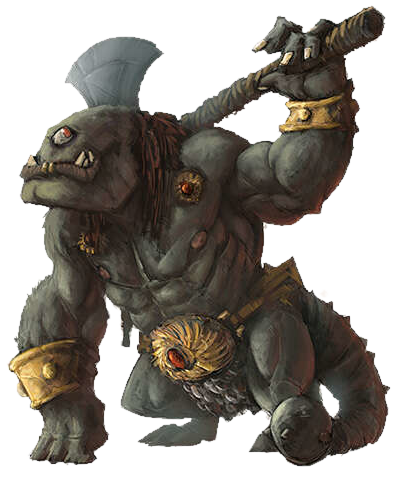
\includegraphics[width=0.47\textwidth]{03mechanics/img/31cyclops.png}
\end{figure}

\subsubsection{Damage Charts}
    \begin{DndTable}[width=\linewidth, header=Bludgeoning]{cX}
        \textbf{d20} & \textbf{Effect} \\
        1     & Roll damage as normal. \\
        2-3   & The next attack against the creature has advantage. \\
        4-6   & Push the creature up to 1.5 meters in any direction. \\
        7-8   & Push the creature up to 4.5 meters in any direction. \\
        9-11  & Attacks against the creature are made with advantage until the start of your next turn. \\
        12-13 & The creature is knocked prone. \\
        14-16 & Push the creature up to 4.5 meters away, and the creature is knocked prone. \\
        17-18 & Roll on the Minor Injury chart.
        If the creature is wearing heavy armor roll on the Major Injury chart instead. \\
        19    & Deal the twice maximum result of your damage dice and roll on the major injury chart. \\
        20    & Deal the maximum result of your damage dice twice, the creature is stunned until the end of your next turn, and roll on the major injury chart.
    \end{DndTable}

    \pagebreak

    \begin{DndTable}[width=\linewidth, header=Piercing]{cX}
        \textbf{d20} & \textbf{Effect} \\
        1     & Roll damage as normal. \\
        2-3   & The creature may only move half its movement speed on its next turn. \\
        4-6   & Roll damage dice twice and use the higher result. \\
        7-8   & The creature's movement speed is zero until the end of its next turn. \\
        9-11  & You can roll one of the weapon's damage dice one additional time and add it to the extra damage of the critical hit. \\
        12-13 & Roll on the minor injury chart with disadvantage. \\
        14-16 & Roll on the minor injury chart. \\
        17-18 & Roll on the major injury chart. \\
        19    & Roll on the major injury chart. \\
        20    & Roll on the minor injury chart, and roll on the major injury chart.
    \end{DndTable}

    \begin{DndTable}[width=\linewidth, header=Slashing]{cX}
        \textbf{d20} & \textbf{Effect} \\
        1     & Roll damage as normal. \\
        2-3   & The creature loses 1d6 hit points at the start of its next turn. \\
        4-6   & Choose one of the creature's arms or legs.
        If you slash one of its legs, its movement speed is halved until the end of its next turn.
        If you slash one of its arms, its attack rolls are made with disadvantage until the end of its next turn. \\
        7-8   & The creature is bleeding.
        For the next minute the creature loses 1d4 damage at the start of each of its turns until it uses two actions to staunch this wound. \\
        9-11  & Wounded, the creature has disadvantage on weapon attack rolls for a minute.
        The creature can roll a Constitution saving throw (DC 15) at the end of each of its turns.
        On a success, it ends this effect. \\
        12-13 & The creature is bleeding.
        For the next minute the creature loses 1d8 hit points at the start of each of its turns until it uses two actions to staunch this wound. \\
        14-16 & The creature is bleeding.
        For the next minute the creature loses 1d12 hit points at the start of each of its turns until it uses two actions to staunch this wound. \\
        17-18 & Roll on the minor injury chart.
        If the creature is wearing light or no armor roll on the major injury chart instead. \\
        19    & Roll on the major injury chart. \\
        20    & Roll on the major injury chart, and the creature is bleeding.
        For the next minute the creature loses 2d8 hit points at the start of each of its turns until it uses two actions to staunch this wound.
    \end{DndTable}

    \newpage

    \begin{DndTable}[width=\linewidth, header=Acid]{cX}
        \textbf{d20} & \textbf{Effect} \\
        1     & Roll damage as normal. \\
        2-3   & You induce temporary anosmia on the creature.
        While in this state, the creature has disadvantage on all Wisdom (Perception) checks that rely on smell.
        This counts as a minor injury. \\
        4-6   & The creature is scarred.
        While scarred the creature has disadvantage on all Charisma ability checks except Charisma (Intimidation).
        This counts as a minor injury. \\
        7-8   & You induce anosmia on the creature.
        While in this state, the creature automatically fails on all Wisdom (Perception) checks that rely on smell.
        Additionally, the creature has disadvantage on checks with Cooking Utensils.
        This counts as a major injury. \\
        9-11  & The creature is disfigured.
        While disfigured the creature has disadvantage on all Charisma ability checks except Charisma (Intimidation).
        This counts as a major injury. \\
        12-13 & The creature's AC is reduced by 1.
        If the creature is wearing armor, it must be repaired for 1/4th of the price of a new armor of the same type to regain its AC modifier.
        If not, this counts as a minor injury. \\
        14-16 & Roll on the minor injury chart.
        Additionally, the creature is disfigured.
        While disfigured the creature has disadvantage on all Charisma ability checks except Charisma (Intimidation).
        This counts as a major injury. \\
        17-18 & The creature's AC is reduced by 2.
        If the creature is wearing armor, it must be repaired for half of the price of a new armor of the same type to regain its AC modifier.
        If not, this counts as a minor injury. \\
        19    & Roll on the major injury chart. \\
        20    & If the creature is wearing armor, the armor is destroyed and roll on the major injury chart.
        If the creature is not wearing armor, roll on the major injury chart and the creature is disfigured.
        While disfigured the creature has disadvantage on all Charisma ability checks except Charisma (Intimidation).
        This counts as a major injury.
    \end{DndTable}

    \thispagestyle{empty} % Remove footer so that it doesn't clash with the image.
    \begin{tikzpicture}[remember picture,overlay]
        \node[anchor=south east, xshift=0.10cm, yshift=-0.10cm] at (current page.south east) {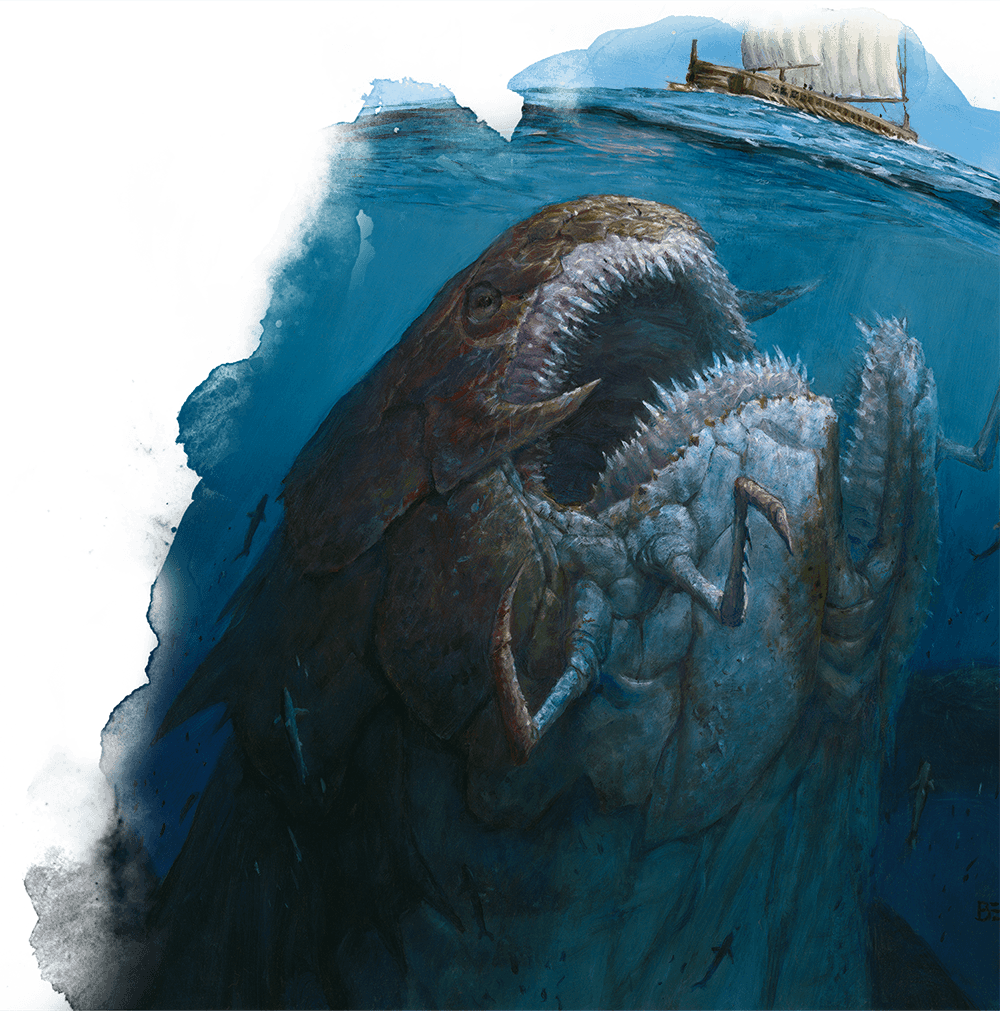
\includegraphics[width=0.5\pdfpagewidth]{03mechanics/img/31friendlyillhevi.png}};
    \end{tikzpicture}

    \newpage

    \begin{DndTable}[width=\linewidth, header=Cold]{cX}
        \textbf{d20} & \textbf{Effect} \\
        1     & Roll damage as normal. \\
        2-3   & The creature may only move half its movement speed on its next turn. \\
        4-6   & The creature has disadvantage on attack rolls until the end of its next turn. \\
        7-8   & The creature’s movement speed is 0 until the end of its next turn. \\
        9-11  & The creature gains vulnerability to bludgeoning damage for a minute. \\
        12-13 & The creature is paralyzed until the end of its next turn. \\
        14-16 & The creature is paralyzed until the end of its next turn.
        If the creature takes damage before the end of its next turn, roll on the minor injury chart. \\
        17-18 & The creature is paralyzed until the end of its next turn and rolls on the minor injury chart. \\
        19    & Roll on the major injury chart. \\
        20    & Roll on the major injury chart, and the creature is paralyzed for the next minute.
        The creature may attempt a Constitution saving throw at the end of each of its turns (DC 15) to end this effect.
        If it fails this saving throw three times it is frozen solid and becomes petrified, but frozen solid rather than turned to stone.
    \end{DndTable}

    \begin{DndTable}[width=\linewidth, header=Fire]{cX}
        \textbf{d20} & \textbf{Effect} \\
        1     & Roll damage as normal. \\
        2-3   & Attack rolls for attacks that deal fire damage have advantage against the creature until the end of its next turn. \\
        4-6   & You burn the creature's hands.
        The creature drops any objects it is holding. \\
        7-8   & The creature is on fire.
        While the creature is on fire it takes 2d4 fire damage at the start of each of its turns.
        The creature can end this condition by dropping prone and using 1.5 meters of movement to roll on the ground. \\
        9-11  &  \\
        12-13 & The creature is on fire.
        While the creature is on fire it takes 2d6 fire damage at the start of each of its turns.
        The creature can end this condition by dropping prone and using 1.5 meters of movement to roll on the ground. \\
        14-16 & The creature is charred.
        If the creature has resistance to fire, it loses that resistance.
        If the creature does not have resistance to fire, it gains vulnerability to fire.
        Both of these effects are considered a minor injury. \\
        17-18 & Roll on the minor injury chart.
        Additionally, the creature is on fire.
        While on fire it takes 2d6 fire damage at the start of each of its turns.
        The creature can end this condition by dropping prone and using 1.5 meters of movement to roll on the ground. \\
        19    & Roll on the major injury chart. \\
        20    & Roll on the major injury chart.
        Additionally, the creature is on fire.
        While the creature is on fire it takes 2d8 fire damage at the start of each of its turns.
        The creature can end this condition by dropping prone and using 1.5 meters of movement to roll on the ground.
    \end{DndTable}

    \begin{DndTable}[width=\linewidth, header=Force]{cX}
        % TODO: Check back here after done with spells. Dunno if we're keeping Force damage.
        \textbf{d20} & \textbf{Effect} \\
        1     & Roll damage as normal. \\
        2-3   & The creature has disadvantage on saving throws against spells until the end of its next turn. \\
        4-6   & The creature is pushed 4.5 meters away from you. \\
        7-8   & Spell attack rolls against the creature have advantage until the end of its next turn. \\
        9-11  & The creature is knocked prone. \\
        12-13 & The creature is spellbound until the end of its next turn.
        While spellbound it makes saving throws against spells with disadvantage and spell attack rolls against it have advantage. \\
        14-16 & The creature is spellbound for the next minute.
        While spellbound it makes saving throws against spells with disadvantage and spell attack rolls against it have advantage.
        At the end of each of the creature’s turns it can make an Intelligence saving throw (DC 12) to end this effect. \\
        17-18 & Roll on the minor injury chart.
        Additionally, the creature is spellbound for the next minute.
        While spellbound it makes saving throws against spells with disadvantage and spell attack rolls against it have advantage.
        At the end of each of the creature’s turns it can make an Intelligence saving throw (DC 15) to end this effect. \\
        19    & Roll on the major injury chart. \\
        20    & Roll on the major injury chart.
        Additionally, the creature is spellbound for the next minute.
        While spellbound it makes saving throws against spells with disadvantage and spell attack rolls against it have advantage.
        At the end of each of the creature’s turns it can make an Intelligence saving throw (DC 18) to end this effect.
    \end{DndTable}

    \begin{DndTable}[width=\linewidth, header=Lightning]{cX}
        \textbf{d20} & \textbf{Effect} \\
        1     & Roll damage as normal. \\
        2-3   & The creature cannot use reactions until the end of its next turn. \\
        4-6   & If the creature willingly moves before the start of your next turn, it takes 1d8 lightning damage. \\
        7-8   & You may choose one other creature within 4.5 m. of the victim.
        That creature must succeed on a Dexterity saving throw (DC 12) or take half as much damage. \\
        9-11  & The creature is paralyzed until the start of your next turn. \\
        12-13 & You may choose one other creature within 4.5 m. of the victim.
        That creature must succeed on a Dexterity saving throw (DC 15) or take half as much damage. \\
        14-16 & Roll on the minor injury chart.
        If the creature is wearing metal armor roll on the major injury chart instead. \\
        17-18 & The creature and all creatures within 4.5 m. of it cannot take reactions until the end of their next turn.
        Then roll on the minor injury chart. \\
        19    & Roll on the major injury chart. \\
        20    & All creatures within 4.5 m. of the victim must succeed on a Dexterity saving throw (DC 18) or take half as much damage.
        Then roll on the major injury chart.
    \end{DndTable}

    \begin{DndTable}[width=\linewidth, header=Necrotic]{cX}
        \textbf{d20} & \textbf{Effect} \\
        1     & Roll damage as normal. \\
        2-3   & The creature cannot regain hit points until the end of its next turn. \\
        4-6   & Choose an ability.
        The creature has disadvantage on ability checks made with the chosen ability for a minute. \\
        7-8   & The creature’s maximum hit points are reduced by an amount equal to the damage dealt.
        This lasts until the creature takes a short rest. \\
        9-11  & You heal yourself an amount equal to half of the damage dealt. \\
        12-13 & The creature’s maximum hit points are reduced by an amount equal to the damage dealt.
        This is considered a minor injury. \\
        14-16 & The creature cannot regain hit points for the next minute.
        It may make a Constitution saving throw (DC 15) at the end of each of its turns to end this effect. \\
        17-18 & The creature’s maximum hit points are reduced by an amount equal to the damage dealt.
        This is considered a major injury.
        Then roll on the minor injury chart. \\
        19    & Roll on the major injury chart. \\
        20    & The creature cannot regain hit points for the next minute.
        It may make a Constitution saving throw (DC 18) at the end of each of its turns to end this effect.
        Then roll on the major injury chart.
    \end{DndTable}

    \begin{DndTable}[width=\linewidth, header=Poison]{cX}
        \textbf{d20} & \textbf{Effect} \\
        1     & Roll damage as normal. \\
        2-3   & The creature has disadvantage on its next ability check, attack roll, or saving throw. \\
        4-6   & The creature stinks.
        It has disadvantage on all Charisma checks except Charisma (Intimidation) and Perception checks that rely on smell.
        This lasts until the creature bathes. \\
        7-8   & The creature has disadvantage on all ability checks, attack rolls, and saving throws until the end of its next turn. \\
        9-11  & Any creature in a radius of 3 meters around the target must roll a Constitution saving throw.
        On a failure, they take half the damage dealt. \\
        12-13 & The creature is poisoned for the next minute.
        The creature may attempt a Constitution saving throw at the end of each of its turns (DC 12) to end this effect. \\
        14-16 & The creature is poisoned for the next minute.
        The creature may attempt a Constitution saving throw at the end of each of its turns (DC 15) to end this effect. \\
        17-18 & Roll on the minor injury chart and the creature is poisoned for the next minute.
        The creature may attempt a Constitution saving throw at the end of each of its turns (DC 18) to end this effect. \\
        19    & Roll on the major injury chart. \\
        20    & Roll on the major injury chart, and the creature is poisoned for the next minute.
        The creature may attempt a saving throw at the end of each of its turns (DC 18) to end this effect.
    \end{DndTable}

    \begin{DndTable}[width=\linewidth, header=Psychic]{cX}
        \textbf{d20} & \textbf{Effect} \\
        1     & Roll damage as normal. \\
        2-3   & You control the creature’s movement on its next turn. \\
        4-6   & The creature cannot differentiate friend from foe until the end of its next turn. \\
        7-8   & Attacks against the creature are made with advantage until the start of your next turn. \\
        9-11  & You control the creature’s actions on its next turn. \\
        12-13 & The creature's mind is broken.
        If the creature has resistance to psychic damage, it loses that resistance.
        If the creature does not have resistance to psychic damage, it gains vulnerability to it.
        Both of these effects are considered a minor injury. \\
        14-16 & You control the creature during its next turn. \\
        17-18 & Roll on the Insanity chart with disadvantage. \\
        19    & Roll on the Insanity chart. \\
        20    & Roll on the Insanity chart with advantage.
    \end{DndTable}

    \begin{DndTable}[width=\linewidth, header=Radiant]{cX}
        \textbf{d20} & \textbf{Effect} \\
        1     & Roll damage as normal. \\
        2-3   & The has disadvantage on any Perception checks that rely on sight.
        This is considered a minor injury. \\
        4-6   & The creature's attack rolls are made with disadvantage. \\
        7-8   & The creature is blinded until the end of its next turn. \\
        9-11  & The creature is blinded for a minute.
        It can make a Constitution saving throw (DC 12) at the end of each of its turns to end this effect. \\
        12-13 & The creature glows for the next minute.
        While glowing it produces bright light up 3 meters and dim light up to 9 meters and all successful attacks against the creature deal an additional 1 radiant damage. \\
        14-16 & The creature is frightened of you for the next minute.
        It can make a Wisdom saving throw (DC 15) at the end of each of its turns to end this effect. \\
        17-18 & Roll on the minor injury chart.
        Additionally, the creature glows for the next minute.
        While glowing it produces bright light up 3 meters and dim light up to 9 meters and all successful attacks against the creature deal an additional 1d4 radiant damage. \\
        19    & Roll on the major injury chart. \\
        20    & Roll on the major injury chart.
        Additionally, the creature glows for the next minute.
        While glowing it produces bright light up 3 meters and dim light up to 9 meters and all successful attacks against the creature deal an additional 1d6 radiant damage.
    \end{DndTable}

    \pagebreak~
    \begin{tikzpicture}[remember picture,overlay]
        \node[anchor=north, yshift=0.10cm] at (current page.north) {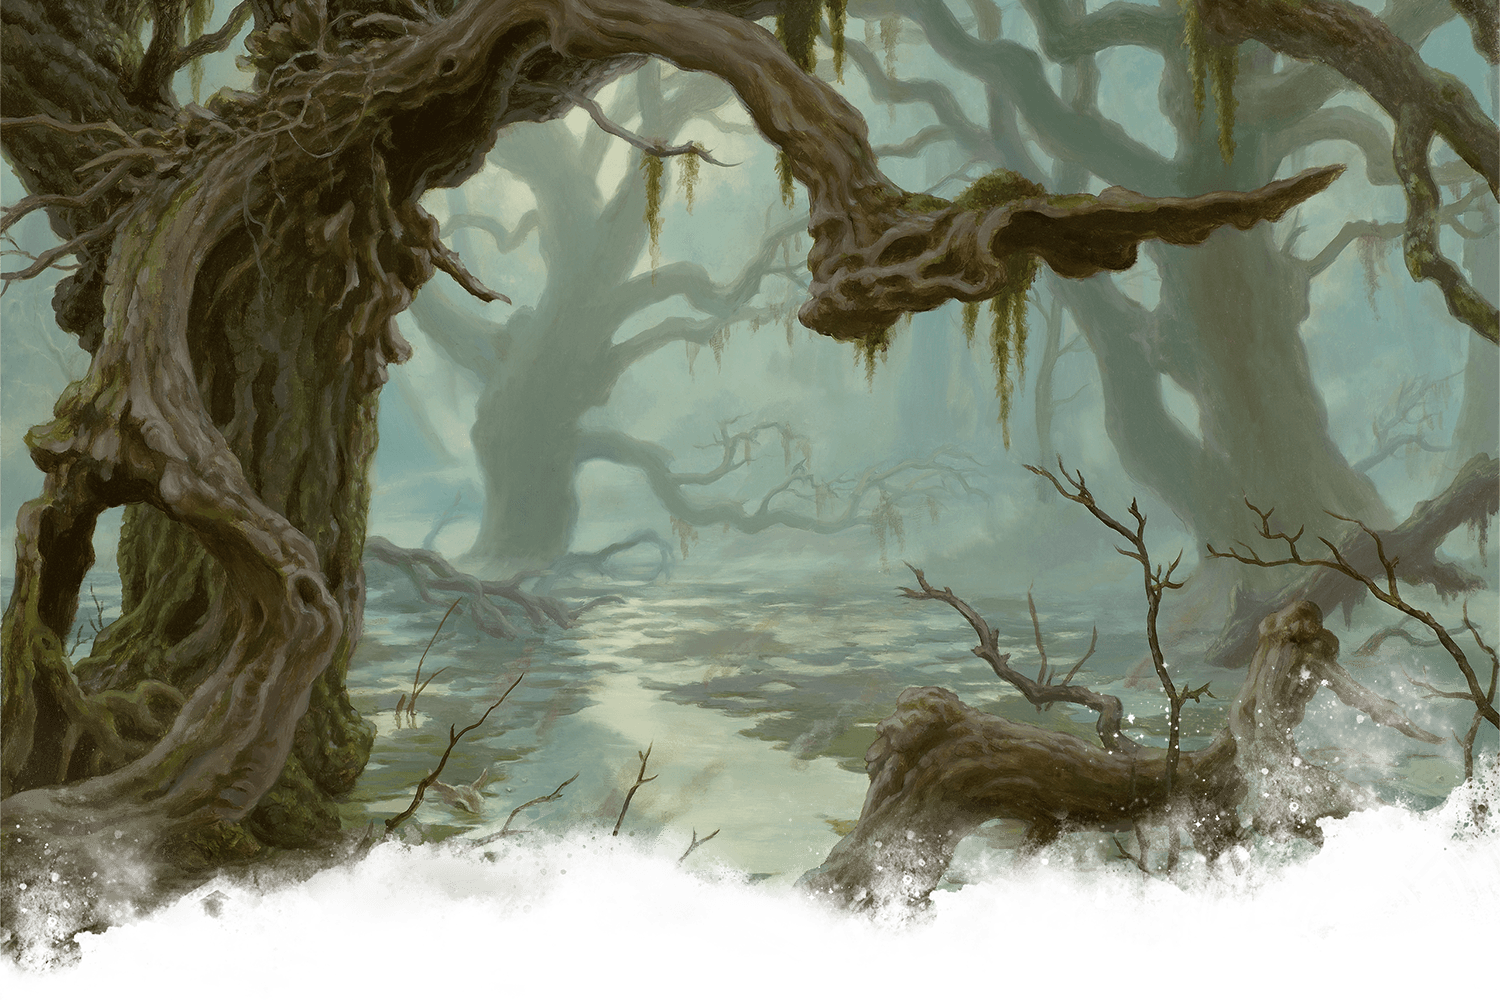
\includegraphics[width=\pdfpagewidth]{03mechanics/img/31arastas_domain.png}};
    \end{tikzpicture}

    \vspace{12.0cm}

    \begin{DndTable}[width=\linewidth, header=Thunder]{cX}
        \textbf{d20} & \textbf{Effect} \\
        1     & Roll damage as normal. \\
        2-3   & The creature has disadvantage on any Perception checks that rely on hearing.
        This is considered a minor injury. \\
        4-6   & The creature is deafened until the end of its next turn. \\
        7-8   & The creature is confused until the end of its next turn.
        While confused, the creature moves in a random direction determined by the DM. \\
        9-11  & The creature is deafened for one minute. \\
        12-13 & The creature is stunned until the start of its next turn and is deafened for one minute. \\
        14-16 & The creature is deafened permanently.
        This is considered a major injury. \\
        17-18 & The creature is stunned until the end of its next turn and is deafened for one minute.
        Then roll on the minor injury chart. \\
        19    & Roll on the major injury chart. \\
        20    & The creature is stunned until the end of its next round and is deafened for one minute.
        Then roll on the major injury chart.
    \end{DndTable}

% !TEX root = ../main.tex

\pagebreak~
\vspace{11.5cm}

\subsection*{Dementia} \label{ssec::dementia}
\DndDropCapLine{H}{arsh is the process that awaits the}
foolish or unlucky enough to lose their qualar.
Their sentience slips away slowly as they lose their mental capacities.
Perhaps the worst part is that inward awareness is one of the last attributes lost, forcing them to be fully conscious of the process.

The road towards dementia comes in seven stages, each roughly lasting a week.
At the moment when you lose your qualar, you enter the first stage of dementia.
After a week, you roll a DC 15 Intelligence saving throw.
On a fail, you enter the next stage of dementia.
On a success, you stay on your current stage and roll again at the start of the next week.
Dementia is unavoidable, and the DC increases by 1 after every successful roll.

\subsubsection{First Stage}
    No obvious signs of dementia, only minor short-memory loss occurs.
    The main symptoms are associated to the anxiety from the loss of the qualar.
    You start focusing more on your past, often drifting away into daydreams.

    You suffer the following effects:
    \subparagraph{Decreased Awareness} You roll for initiative and Dexterity saving throws with disadvantage.
    \subparagraph{Restlessness} Roll an DC 12 intelligence saving throw right after a short rest.
    On a success, you recover your hit points normally.
    On a failure, you only recover half of the hit dice rolled (rounded down).

\subsubsection{Second Stage}
    The self realization and awareness that something is wrong settles in.
    You refuse to accept that your mind is slipping away.
    The more effort you put on remembering the more deterioration your memory suffers.
    Confusion starts setting in.

    In addition to the effects of the first stage, you suffer the following effects:
    \subparagraph{Lack of Recollection} Any ability check made to remember or recollect a memory is done with disadvantage.
    All Intelligence (History) checks are made with disadvantage.
    \subparagraph{Mood Swings} All Charisma ability checks and saving throws are made with disadvantage.

\subsubsection{Third Stage}
    You experience increased forgetfulness and might find concentrating difficult.
    You are presented with some of the last coherent memories before confusion fully rolls in.
    Some singular memories become more disturbed, isolated, broken, and distant.
    These are the last embers of awareness.

    In addition to the effects of the last stages, you suffer the following effects:
    \subparagraph{Decreased Concentration} All Constitution saving throws made to maintain concentration are made with disadvantage.
    \subparagraph{Vagrant Mind} Intelligence and Wisdom ability checks and saving throws are rolled with disadvantage.

\subsubsection{Fourth Stage}
    Grey mists form and fade away in your memory.
    The ability to recall singular memories gives way to confusion and horror.
    You struggle with daily tasks, presenting clear cognitive problems.

    In addition to the effects of the last stages, you suffer the following effects:
    \subparagraph{Motor Difficulties} Strength and Dexterity ability checks and saving throws are rolled with disadvantage.
    Attack rolls are made with disadvantage.
    \subparagraph{Drifting Conscience} In combat, roll a DC 8 Intelligence saving throw at the start of every turn.
    On a failure, you forget where you are, and cannot take any actions during the turn.

\subsubsection{Fifth Stage}
    You have major memory deficiencies.
    The few lapses of consciousness you get are filled with dread, as you realize your mind has mostly left you.
    The repetition and rupture gives way to calmer moments, as the unfamiliar becomes familiar.

    In addition to the effects of the last stages, you suffer the following effects:
    \subparagraph{Loss of Fortitude} All rolls are made with disadvantage.
    \subparagraph{Complete Unawareness} All Intelligence (Investigation), Wisdom (Insight), and Wisdom (Perception) automatically fail.
    Your passive investigation, insight, and perception become 0.

\subsubsection{Sixth Stage}
    Your mental state is beyond description.
    You struggle to remember your early life, even forgetting the names of your family and fellows.
    Your capacity of speech is severely impaired, and you suffer sudden and radical personality and emotional changes.

    In addition to the effects of the last stages, you suffer the following effects:
    \subparagraph{Declining Speech} You automatically fail all Charisma ability checks and saving throws, and have a very hard time communicating verbally.
    \subparagraph{Hope Lost} As your conscious mind fights your natural tendencies, you automatically fail death saving throws.

\subsubsection{Final Stage}
    Everywhere, an empty bliss.

    You make what will most likely be your last die roll.
    Nothing can give you advantage or disadvantage on this roll.
    Roll a d20 on the post-dementia table.
    You suffer the effect rolled.

    \begin{DndTable}[width=\linewidth, header=Post-dementia Effects]{lX}
        \textbf{Roll} & \textbf{Effect} \\
        1 & Your last emotion is rage.
        You become mindless and violent, attacking your companions without reason. \\
        2-5 & Your last emotion is apathy.
        You mindlessly stare to the east until you die of natural causes. \\
        6-18 & Even after brain death, you seek survival.
        You wander off, attacking any who try to stop you.
        You become a lost one. \\
        19 & With memories gone, your mind is fully pulled by its tidal impulses.
        You lose control of your character, who becomes a servant of The Sorrow. \\
        20 & Recovery from dementia is very rare, but not impossible.
        You recover from all effects associated to dementia, and gain the \textbf{Demented Insight} feat at page \pageref{feat::dementedinsight}.
    \end{DndTable}

    The only conventional way to remove dementia is to obtain a qualar again.
    When this happens, you quickly recover your sentience.
    Each morning, you reduce your stage of dementia by one, and don't need to roll the Intelligence saving throw associated to the status.


% \subsection*{Encumbrance} \label{ssec::encumbrance}
%     \textbf{TODO.}
% NOTE: We can stay with vanilla's system, it's good enough tbh.

\pagebreak~
\begin{tikzpicture}[remember picture,overlay]
    \node[anchor=north, yshift=0.10cm] at (current page.north) {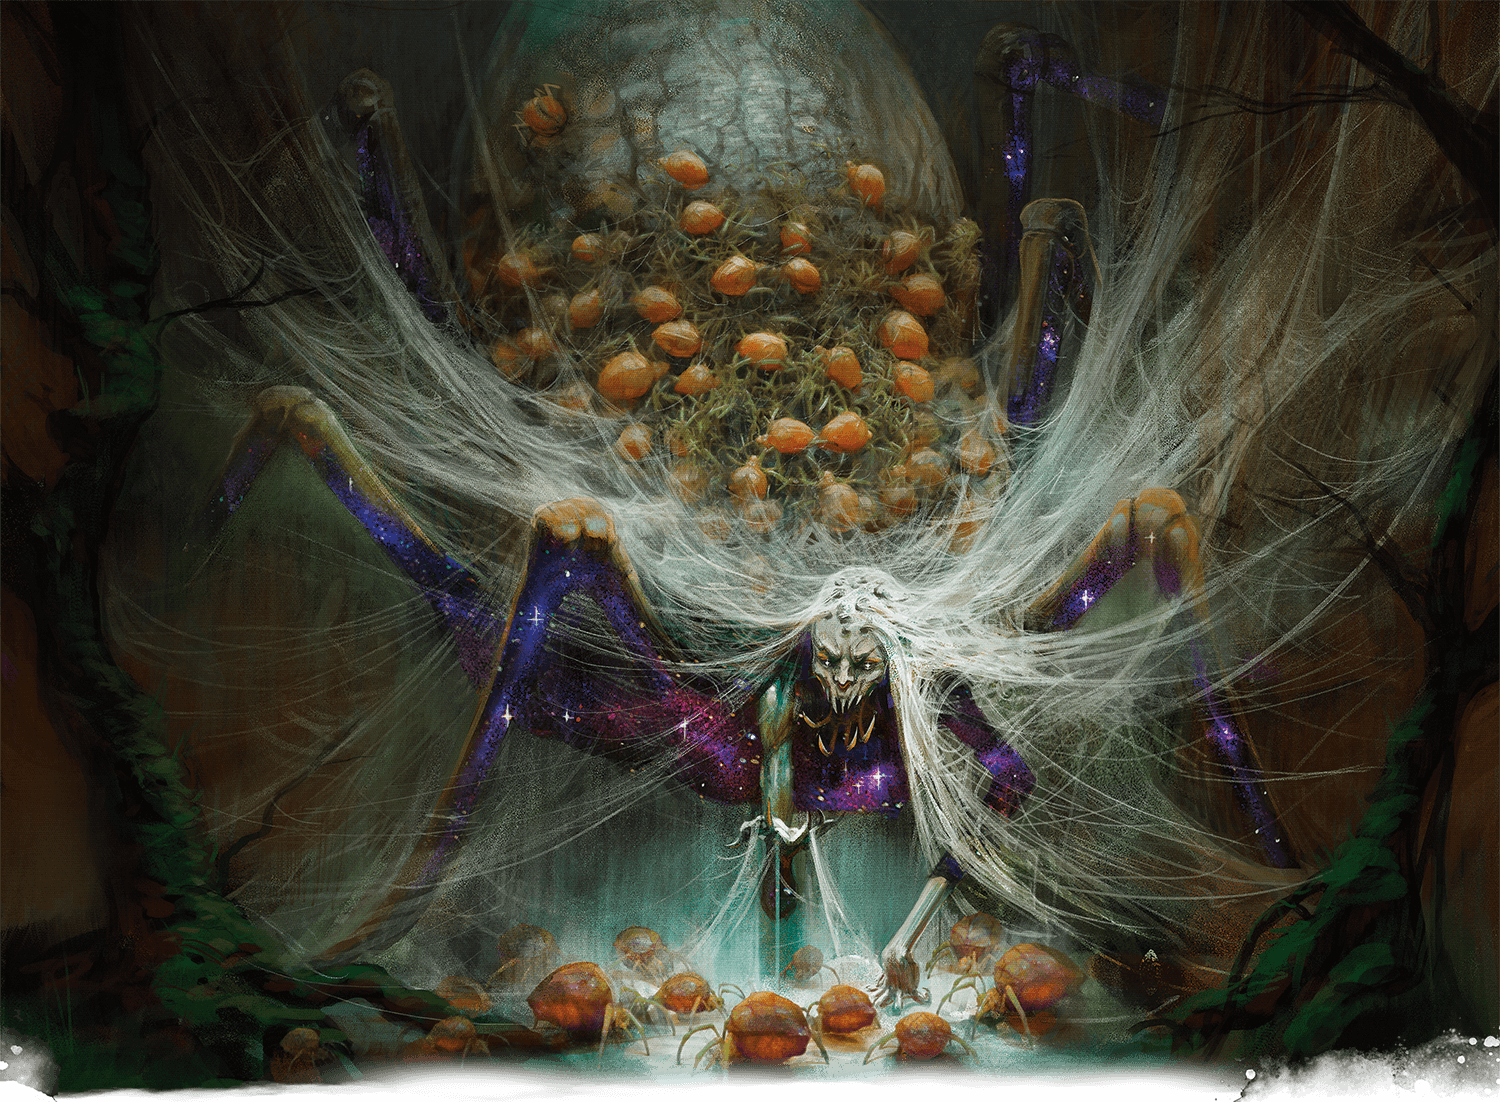
\includegraphics[width=\pdfpagewidth]{03mechanics/img/30arastaoftheendlessweb.png}};
\end{tikzpicture}

\vspace{14.0cm}

\subsection*{Flaws} \label{ssec::flaws}
    As you travel through treacherous lands and fight dangerous creatures, it is natural to acquire permanent wounds or fears.
    These new flaws don't need to be entirely bad --- they reflect a changing point in your life, and can be beneficial in their own way.

    When you suffer a major injury, fear, or insanity, you can choose to accept this effect as a flaw.
    When you do so, it becomes permanent.
    For example, a crippled arm might need to be severed off, or your character might get used to their insanity and learn to live with it instead of treating it.

    While this effect may prove as a permanent hindrance to you, you are rewarded with FP for taking it.
    This extra FP does not count towards your level.
    The number of FP awarded by effects is specified in the effect's description.

% \subsection*{Hunger and Thirst} \label{ssec::hungerandthirst}
%     \textbf{TODO.}
% NOTE: We can stay with vanilla's system, it's good enough tbh.

\pagebreak~
\vspace{11.5cm}

\subsection*{Injuries \& Insanity} \label{ssec::injuriesandinsanity}
    Critical hits or especially severe events can cause injuries or insanity.
    When a creature suffers a minor injury it can be healed by someone competent with a healer's kit over the course of a long rest.
    Major injuries and Insanities require assistance from a dedicated healer, or someone with the relevant feat (see page \pageref{feat::physician} and \pageref{feat::therapist}).

    Alternatively, you can decide to keep an injury or insanity as a new Flaw (see page \pageref{ssec::flaws}) during a short rest after it is applied.
    Minor injuries and insanities award you 2 FP, while major injuries award you 3 FP.
    Acquiring a flaw from a major injury related to a minor injury you already have (such as Crippled Leg and Injured Leg) only awards 1 FP --- one more than what you already had gained.
    % The text of certain injuries will specify other ways this injuries might resolve.

    \pagebreak

    \begin{table*}[t]
        \begin{DndTable}[width=\linewidth, header=Minor and Major Injuries]{cXX}
            \textbf{d20} & \textbf{Minor Injury} & \textbf{Major Injury} \\
            1-3 &
            \textbf{Injured leg}.
            Your movement speed is reduced by 2 meters. &
            \textbf{Crippled leg}.
            Your movement speed is reduced by 2 meters, and you have disadvantage on Dexterity saving throws. \\
            4-8 &
            \textbf{Injured arm}.
            One of your arms (randomly determined) cannot be used to hold a shield, and you have disadvantage on any rolls involving the use of that arm. &
            \textbf{Crippled arm}.
            One of your arms (randomly determined) cannot be used to hold an item, and any ability check or attack roll requiring that arm automatically fails. \\
            9-11 &
            \textbf{Multiple injuries}.
            Your maximum hitpoints are reduced by an amount equal to half of the damage dealt by the attack. &
            \textbf{Severely wounded}.
            Your maximum hit points are reduced by an amount equal to the damage dealt by the attack. \\
            12-16 &
            \textbf{Badly beaten}.
            You have disadvantage on Constitution saving throws. &
            \textbf{Edge of death}.
            You have disadvantage on Constitution and death saving throws. \\
            17-19 &
            \textbf{Ringing blow}.
            You are stunned until the end of your next turn, and you are deafened. &
            \textbf{Blinding blow}.
            You are blinded. \\
            20    &
            \textbf{Blow to the head}
            You are unconscious for 2d12 hours. &
            \textbf{Decapitated}.
            You are dead.
        \end{DndTable}
    \end{table*}

    \thispagestyle{empty} % Remove footer so that it doesn't clash with the image.
    \begin{tikzpicture}[remember picture,overlay]
        \node[anchor=south west, xshift=-0.10cm, yshift=-0.10cm] at (current page.south west) {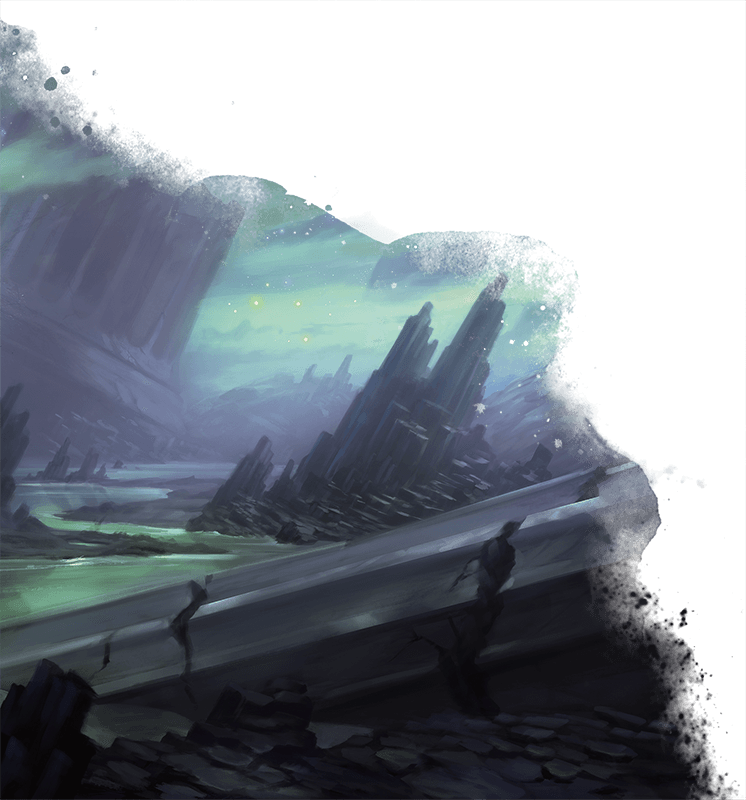
\includegraphics[width=0.5\pdfpagewidth]{03mechanics/img/30outerlands.png}};
    \end{tikzpicture}

\subsection*{Only One Chance} \label{ssec::onlyonechance}
    As a rule, you only have one chance to succeed in any action.
    Once you have rolled the dice, you many not roll again to achieve the same goal.
    You need to try something different or wait until the circumstances have changed in a substantial way.
    Or, you know, let another PC try.

    This rule does not apply to combat, where you can attack the same enemy until it becomes a bloody pulp.

\subsection*{Opportunity Attacks} \label{rule::opportunityattacks}
    In a fight, everyone is constantly watching for enemies to drop their guard.
    While heedless movement is easily punished, any lack of concentration or unplanned action can have devastating consequences.
    Various actions provoke opportunity attacks from a creature:
    \begin{itemize}
        \item Moving out of the creature's reach.
        This doesn't apply when someone or something moves you without using your movement, action, or reaction.

        \newpage

        \item Picking up an item from the floor while in the creature's reach.
        \item Unsheathing a weapon while in the creature's reach.
        \item Donning or doffing a shield while in the creature's reach.
        \item Using the Attack action with a ranged weapon or spell attack in a creature's reach.
    \end{itemize}
    You can avoid opportunity attacks during your turn by taking the Disengage action.

\subsection*{Short and Long Rests} \label{ssec::shortandlongrests}
    The gritty campaigns in Yuadrem benefit from longer rest times.
    Short rests last for 8 hours, and long rests for 3 days --- half a week in the Fagalian calendar.
    This puts the brakes on the campaign, requiring the players to carefully judge the benefits and drawbacks of combat.
    % Characters can't afford to engage in too many battles in a row, and all adventuring requires careful planning.

    Complementing this optional rule is the fact that all spell slots are recovered during short rests, and a short rest removes one level of exhaustion.
    Additionally, all the systems in this book are designed with this optional rule in mind, so some things need to be re-balanced if a group is to play without this rule.

    \begin{table*}[h]
        \begin{DndTable}[width=\linewidth, header=Insanity]{cX}
            \textbf{d20} & \textbf{Insanity} \\
            1  & \textbf{Synesthesia}.
            You can hear colors, smell sounds, or taste textures. Regardless of the specific manifestation, you have disadvantage on all Perception and Investigation skill checks. \\
            2  & \textbf{Kleptomania}.
            Once per day when you are in a personal residence or marketplace, the DM can call on you to succeed on a Wisdom saving throw (DC 12) or attempt to steal an item of insignificant practical and monetary value. \\
            3  & \textbf{Paranoia}.
            Once per day following an interaction with another creature (including other PCs) the DM can call on you to succeed on a Wisdom saving throw (DC 12) or you suspect that creature is secretly plotting against you. \\
            4  & \textbf{Obsession}.
            Choose a person or personal interest you are obsessed with. Once per day, when you are presented with an opportunity to interact with or learn more about the subject of your obsession the DM can call on you to succeed on a Wisdom saving throw (DC 14) or ignore everything else to obsess over the object of your fascination. \\
            5  & \textbf{Addiction}.
            Choose a behavior or substance you have used. Once per day, when you are presented with an opportunity to do the behavior or use the substance the DM can call on you to succeed on a Wisdom saving throw (DC 14) or ignore everything else to indulge in your vice. \\
            6  & \textbf{Odd Thinking}.
            Once per day when you hear a rational explanation for an event or occurrence, your DM may call on you to succeed on a Wisdom saving throw (DC 12) or you reject the rational explanation for a conspiratorial or fantastical explanation. \\
            7  & \textbf{Narcissism}.
            When you take an action or series of action that doesn’t directly benefit you, you must pass a Wisdom saving throw (DC 11) or you can’t take that action / series of actions.
            If any self-sacrifice on your part would be required the DC of the saving throw is increased to 16. \\
            8  & \textbf{Delusional}.
            When you gain this insanity the DM will tell you a belief that you have. No matter what evidence is presented to the contrary so long as you have this insanity you cannot be persuaded that this belief is not true. \\
            9  & \textbf{Pica}.
            Once per day the DM can call on you to pass a Wisdom saving throw (DC 14) or immediately eat one non-food object (such as dirt, napkins, or a small piece of jewelry) of the DM’s choice. \\
            10 & \textbf{Retrograde amnesia}.
            You forget everything about your personal life prior to the moment you received this insanity. \\
            11 & \textbf{Overwhelmed}.
            If you do not have immunity or resistance to psychic damage, you gain vulnerability to psychic damage.
            If you have resistance to psychic damage, you lose it.
            If you have immunity to psychic damage, you lose it but gain resistance to psychic damage. \\
            12 & \textbf{Anterograde amnesia}.
            Whenever you try to recall a fact you learned since you received this insanity, make a Intelligence saving throw (DC 12).
            If you fail you cannot recall the fact. \\
            13 & \textbf{Dependence}.
            You must pass a Wisdom saving throw (DC 14) to take an action that one or more of your allies disapprove of. \\
            14 & \textbf{Anxious}.
            You have disadvantage on saving throws against being frightened.
            Additionally, once per day the DM can call on you to succeed a Wisdom saving throw (DC 14) or be frightened by a creature of the DM’s choosing for the next minute. \\
            15 & \textbf{Mute}.
            Whenever you wish to speak allowed (including casting a spell that has verbal components) you must succeed on a Wisdom saving throw (DC 13) to do so. \\
            16 & \textbf{Narcolepsy}.
            You have disadvantage on saving throws against sleeping or unconsciousness.
            Once per day the DM may call on you to succeed on a Constitution saving throw (DC 12) or fall unconscious for one minute or until you take damage or another creature spends their action trying to rouse you. \\
            17 & \textbf{Insomnia}.
            You cannot take long rests and your short rests take 8 hours to complete. \\
            18 & \textbf{Homicidal}.
            After each long rest you must pass a Wisdom saving throw (DC 14) or be overcome with the urge to end the life of a humanoid creature and you cannot benefit from another long rest until you do so. \\
            19 & \textbf{Suicidal}.
            After each long rest you must pass a Wisdom saving throw (DC 12) or make an attempt to end your own life. \\
            20 & \textbf{Catatonia}.
            You are unconscious for 10d10 years.
        \end{DndTable}
    \end{table*}

\subsection*{Stress} \label{ssec::stress}
    Adventuring is dangerous, and no matter the amount of heroic deeds in your past you are bound to accumulate stress over time.
    As a mechanic, stress adds long-term consequences to traumatic experiences and tense situations.

    Whenever you drop to 0 hit points, add a point to your stress meter.
    % Some specific attacks directly produce stress on a creature.
    When you reach 4 stress points, you roll on the Afflictions table and acquire the specified affliction, reducing your stress meter back to 2.
    % Afflictions are detrimental conditions that have short or long-term consequences for you.

    Taking a long rest or engaging in downtime activities reduces your stress meter by 1.
    Additionally, some feats like Soothing Presence (see page \pageref{feat::soothingpresence}) and Reliever (see page \pageref{feat::reliever}) add the capacity to reduce stress in different scenarios.

    \newpage~\newpage~\newpage

    \begin{table*}[t]
    \begin{DndTable}[width=\linewidth, header=Affliction]{cX}
        \textbf{d20} & \textbf{Affliction} \\
        1     & \textbf{Insanity}.
        Your mind collapses and you fall into insanity.
        Roll on the Insanity table (see page \pageref{ssec::injuriesandinsanity}) and acquire the rolled insanity. \\
        2-5   & \textbf{Phobia}.
        Powerless at the face of death, you can only watch as your foe strikes its final blow against you.
        You add to your flaws the phobia of the type of creature who put you unconscious.
        Any time you encounter this type of creature, roll a DC 16 Wisdom saving throw at the beginning of each of your turns.
        On a failure, you become frightened of the creature.
        This flaw is permanent, and awards you 1 FP. \\
        6-7   & \textbf{Fearful}.
        % Scared of death, you become fearful and meek.
        Whenever you take damage, roll a DC 12 Wisdom saving throw.
        On a failure, you become frightened of the attacking creature.
        You can repeat this saving throw at the end of each turn.
        This effect lasts until you finish a short rest. \\
        8-9   & \textbf{Paranoid}.
        Whenever you are targetted by a friendly creature for any effect, roll a DC 12 Wisdom saving throw.
        On a failure, you refuse what your ally is offering, be it healing, aid, etc.
        If you ally spent any resource or action on this effect, they are spent anyway.
        This effect lasts until you finish a short rest. \\
        10-11 & \textbf{Selfish}.
        You cannot heal or aid an ally in any way.
        This effect lasts until you finish a short rest. \\
        12-13 & \textbf{Masochistic}.
        Your AC is reduced by 2, and you cannot take the Dodge or Disengage actions.
        This effect lasts until you finish a short rest. \\
        14-15 & \textbf{Abusive}.
        You cannot heal or aid an ally in any way, and you refuse to receive any healing or aid from any creature.
        This effect lasts until you finish a short rest. \\
        16-17 & \textbf{Hopeless}.
        Attacks against you are made with advantage, and you roll saving throws with disadvantage.
        This effect lasts until you finish a short rest. \\
        18-19 & \textbf{Irrational}.
        At the beginning of each of your turns, roll a DC 15 Wisdom saving throw.
        On a failure, you cannot take any action during your turn.
        This effect lasts until you finish a short rest. \\
        20    & \textbf{Virtuous}.
        Stalwart against adversity, your time at death's door only enhances your resolution.
        Your stress meter is reduced to 0, and any ally that can see or hear you has their stress meter reduced by 1.
        Additionally, you have advantage on attack rolls and saving throws for one hour.
    \end{DndTable}
    \end{table*}

    \thispagestyle{empty}
    \begin{tikzpicture}[remember picture,overlay]
        \node[anchor=south, yshift=-0.10cm] at (current page.south) {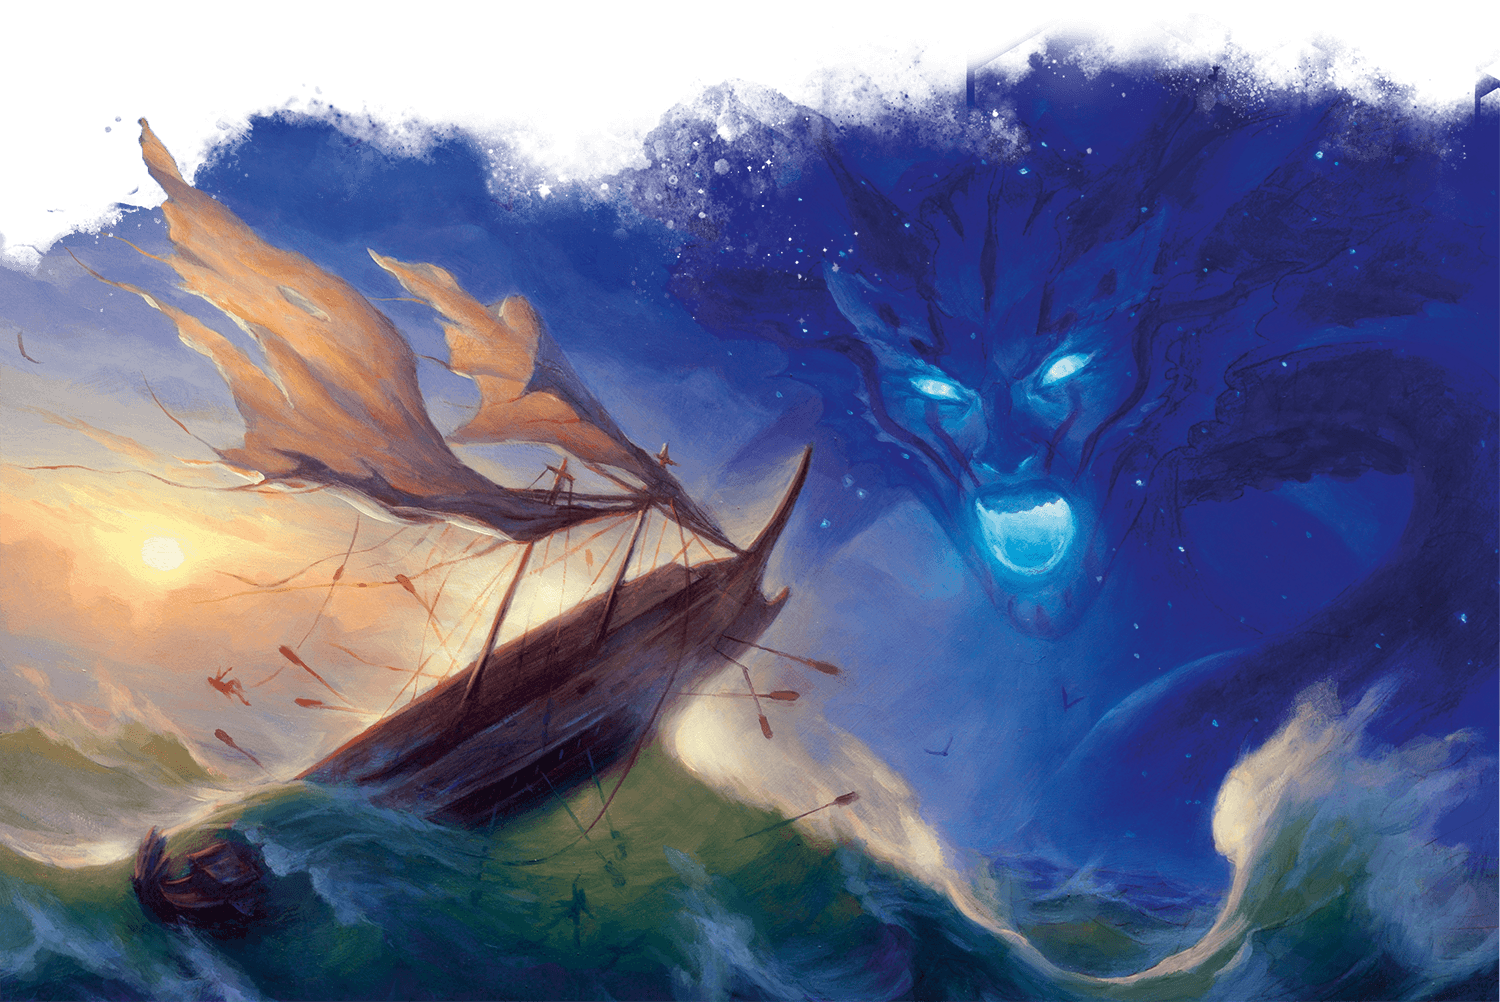
\includegraphics[width=\pdfpagewidth]{03mechanics/img/30thassaangry.png}};
    \end{tikzpicture}


    % !TEX root = ../main.tex
\chapter{Kins} \label{ch::kins}
\DndDropCapLine{C}{ountless millennia before any of the}
modern kins were born, the ets were born into the land of Yuadrem.
% They were named by the other kins, their creations, due to their impressive size.
They were commonly known as the tall kin, for they usually stood well beyond 3 meters.
Their skin was of a pallid, almost bluish white color, and their eyes were as black as the abyss.
% Most ets didn't have any hair.

The species greatly developed their technology, which was biological in nature.
Free from aging and illness, they developed astonishing physical capabilities despite their apparent frailty.
Each et was indeed capable of shaping their own flesh, causing a great variety of characteristics in the many members of the kin.

Ets were obsessed with their individuality, and it was common for them to change their own appearance, molding their flesh to reflect their personality and philosophy.
Despite their longevity however, it was rare for new ets to be born, and the kin never grew to more than a few thousand members.

\subsubsection{Schools of Thought}
Their longing for longevity led them to study the cosmos, trying to find meaning in the stars.
These studies manifested in the form of the schools of thought, large organizations representing different ways of thinking about the cosmos and oneself.
These schools were their main form of government.%, where individuals were represented by their schools.

Among these organizations, the church of Ukarilth was of special significance.
More than a thousand years ago, an event known as the first communion took place.
During a pilgrimage to the dead sea, the et Ukarilth found the deceased embryo of a species yet unknown to its kin, which the tall one dubbed ``the higher kin''.

In an attempt to understand this newfound race, the tall one fused their body with that of the higher one.
The ritual was successful, but it transformed Ukarilth to an insane, shapeless blob.
Later, the church of Ukarilth was born to attempt communication with the mad et.

As the gospel of Ukarilth spread, the kin became convinced that they were utterly insignificant to the cosmos.
The fear caused by this thought elevated their pursuit of individuality.
They believed that the higher kin held a method to become significant, and their schools of thought shifted their studies to focus solely on this strange species.
They believed that with this study they would attain something they called ``the rapture'', described as an ascension to a higher plane of existence.

Their unwavering pursuance eventually led to the schism.
The schism is the most devastating event in Yuadrem's history, causing a 40 year long famine and scarring the land itself for the centuries to come.

\subsubsection{Language}
The tall kin spoke a very sophisticated language, known as jan-theth rlin, simplified as jantherlin.
This language allowed for a very profound expression of one's emotions and inner state, and is still used in poetry to this date.
For when deeper communication is needed, ets could meld their bodies and share thought, but the practice was only used in special rituals or to express especially complex abstract concepts.

As for written word, it was customary for the tall kin to chisel the stone, commonly carving a great variety of images alongside the text.
While this written language originates from jantherlin, each tall one had its own personal version of it.
Other ets could only comprehend one's writing as much as they understood the writer.
This makes the study of jantherlin extremely difficult to modern archaeologists.
% This makes the reading of the jantherlin extremely difficult for the kin that remain in the world, since understanding a particular tall one's scribbles essentially requires understanding their own version of the language.

\begin{figure}[t]
    \centering
    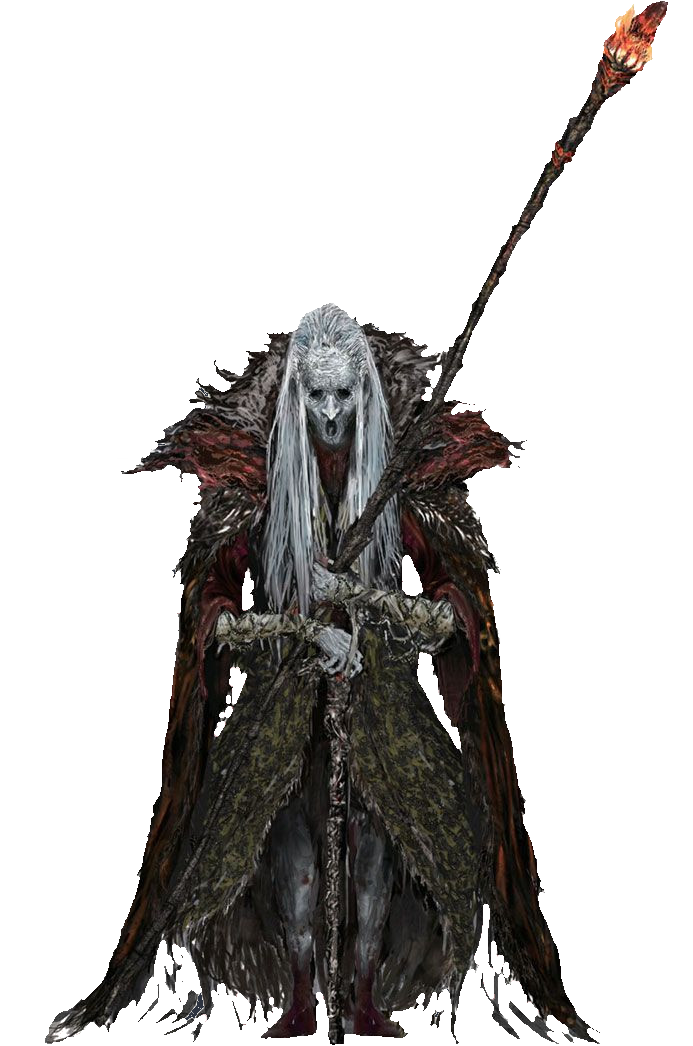
\includegraphics[width=0.45\textwidth]{04kins/img/10et_cleric.png}
\end{figure}

% \subsubsection{Relationships}
% Either by accident or by conscious decision, the tall kin created many of the modern peoples in experiments and studies.
% Most of these held a very high regard for the ets, with some even building entire churches to them.
% However, after it was learned that the they were responsible for the schism, all churches were forcibly shut down, and any adoration is severely punished.


% !TEX root = ../main.tex
\section{Horned Kin} \label{kin::gat}
\DndDropCapLine{W}{hen you contract a horned one, be}
\textit{sure to pay them double.
Fulfill all their needs as they seclude into their workshop, and pay no mind to their uncanny silence.
Most of all, be sure to avoid interrupting them.
Just wait.
The prize that will arrive after they're done working is sure to outshine all your other possessions, and hold a special place in your collection for you and your descendants.}

\hspace*{\fill} --- Orr, Vesjen's master smith.

Citadels carved into the highest of cliff faces.
Mines hidden inside the deepest of ravines.
Workshops rumbling with the sound of hard labor until the darkest of hours.
These are the traits that define the gat.

The gat, marheth'llal rlue, or horned kin are the oldest among the sentient races created by the ets.
Molded as diggers and laborers, their passion for work is ingrained into their very blood.
To date they are known as master miners, builders, and artisans.

Being the first of the kins, they are established and well-developed.
Gats are the builders of the Seven Kingdoms of the Coast, the oldest active nations in Yuadrem.

\subsection*{Beard and Horns}
    The horned kin was designed in the image of goats, and share their horns, facial features, and digitigrade feet.
    They stand in a hunched manner and are generally slender.
    Gats are covered by a thick layer of fur ranging in hues from light blonde to absolute black.
    Many enjoy growing a beard.

    Gats' eyes are of strong colors, usually light blue, yellow, orange, or light brown.
    Like goats, their pupils are rectangular and elongated.
    The manner in which each gat's beard and horns grow is unique, and most take pride in these features, showing them off whenever possible.

    Gats are genderless creatures.
    All gats are born with a pair of seeds hidden in a small sack between their legs.
    Around the age of 30, a gat reaches physical maturity.
    This is signalled by a slight swelling in these seeds, which they can now cut and plant under a thick layer of rich soil.

    While underground, the seed will grow by leeching nutrients off the earth.
    After a gestation period of around 2 years, the gat will dig their way up from the ground and emerge as a somewhat competent infant.
    A gat would-be-parent must always be careful about where to plant their seed, for if a newborn sees the sun or any strong light during their first days, they run the risk of being permanently blinded.

\subsection*{Adaptable and Hardy}
    Gat share many traits with the common goat.
    They dwell on bleak mountaintops, deep ravines, rocky hills, and open plains.
    While adult gats are not sensitive to sunlight, most prefer dark places.
    These predilections lead to gat towns and cities being built underground or in harsh cliff faces.

    Never satisfied with their homes, the horned kin's hubris leads to their cities to reach depth and size.
    Raids against smaller gat city-state are common, and the gats take them as a chance to test their impenetrable defenses, complex traps, and combat-hardened military skills.

\subsection*{Peaceful Demeanor}
    The horned kin are peaceful creatures and mostly shun external conflict.
    They are very sociable creatures, and all city-states have one large marketplace in their center for merchants and caravans to settle in.
    Surrounded by inns and taverns, these markets act as the commerce hubs of the city.

    Community lifestyle is very important to gats, and most wouldn't flinch to give their lives for their city-state.
    Due to the gats' slow reproductive cycle, their cities are very welcoming to other species.
    It's common to find cities and towns where less than half of the total population is gat.
    They treat other species as kin, but high political and military ranks are exclusive to gats.

\subsection*{Impulse towards Greatness}
    It is rare for a gat to willingly leave their home, and most spend their entire lives in one city-state.
    However, some do feel the call to adventure, and most follow it to gather rare crafting materials or to fulfill a task needed by their community.

    Gats are meticulous individuals, and this naturally extends to adventurers.
    They won't step into the wilderness unprepared, sparing no expense in armor, weapons, utilities, and the training to use all of this.

    Gats are naturally family-oriented, and its very rare for one gat to abandon their progeny.
    In the rare occasion that a gat does decide to leave their community behind, it is written law to leave one child or seed planted back home.

    This tradition serves a double purpose.
    First, the child acts as a magnet to their parent.
    Second, in the event that the child is orphaned, their mere presence at least maintains a steady population number.
    These gats are the ``Children of the Collective'', and it is tradition that they are taken care of by the whole city, thus nurturing a strong sense of community.

\subsection*{Gat Names}
    All gat tongues are simple and practical languages, and the horned ones have a tendency towards easy to pronounce names.
    A parent gives their child their name once they gain independence, and its rare for a gat to change it.
    Gats don't use family names, preferring instead to wear their main profession as a surname.

    \paragraph{Names}
    Adrevik, Ani, Anush, Armen, Avag, Gagik, Garen, Gevog, Gohar, Grigor, Hak, Harig, Hovsep, Jirar, Kevon, Khadzak, Marim, Narek, Pagran, Poghos, Ruben, Sivadr, Sona, Vahagn, Vefan.

    \paragraph{Surnames}
    Axgat, Bonecarver, Bowyer, Caretaker, Cook, Dyer, Engraver, Farmer, Fishergat, Glassblower, Gemcutter, Guard, Mason, Metalsmith, Miner, Speargat, Trader, Trapper, Weaponsmith, Woodworker.

\subsection*{Traits}
    Your gat character's hardiness and tendency towards craftsmanship gives them the following set of skills:

    \subparagraph{Ability Score Increase} Your Constitution score increases by 2.

    \subparagraph{Age} Gats mature slowly, but they live very long lives.
    You are sexually mature at around 30 years, and live to around 350 years.

    \subparagraph{Alignment} Industrious and strong, gats focus more on getting things done rather than morals or ethics.
    They have a tendency towards fairness and justice, and therefore are inclined towards the indigo tide.

    \subparagraph{Size} Gats typically range from 1.2 to 1.5 meters.
    Your size is medium.
    They aren't too slender or stout for their size, weighing on average 50 kg.

    \subparagraph{Speed} Your base walking speed is 6 meters.

    \subparagraph{Stable Footing} You are not slowed by difficult terrain caused by rocks, gravel, sheer faces, and other such obstacles.

    \subparagraph{Keratin Horns} You know the Push action (See page \pageref{act::push}), using your strong horns to shove your target.

    Additionally, your horns are a melee weapon that deals 1d4 plus your Strength modifier in bludgeoning damage.

    \subparagraph{Craftsgatship} You are competent with a set of artisan's tools of your choice.

    \subparagraph{Strange Mood} Periodically, individual gat are struck with an idea for a masterwork artifact and enter a strange mood.
    Only with a great force of will can a gat ignore this pull, and not even the strongest can fully stop the craving.

    If you are at least 30 years old, roll a d100 whenever you take a long rest.
    % You can choose to roll this twice.
    On a 100, you are struck by a strange mood.
    The materials required for your masterwork item can either be chosen by you or by the DM.
    They must be related to the proficiency given by your Craftsgatship trait and at least one of them must be either hard to find or very expensive.

    At the start of every subsequent long rest, you must succeed on a Wisdom saving throw of a DC equal to 8 + the number of months since your strange mood started.
    On a fail, the need to work on your craft consumes you.
    If you fail to work on the object in any way during the long rest, your restlessness prevent you from gaining its benefits.

    It takes you a month of work in total to craft the artifact, which can be paused between

    It takes you 2 months of work to craft the artifact, but after you start you can indefinitely pause the production as long as you can properly secure it.
    The masterwork item produced has a value of 100,000 GP, but it's very rare to see a gat willingly part with it.
    These items are usually declared as family heirlooms, personal keepsake, or an offering to a king, leader, or deity.

    Weapons, armor, or similar objects crafted in a strange mood are +2, and are of specially exquisite quality.

    \subparagraph{Languages} You know how to speak, write, and read Avshenese and one additional language of your choice.

\begin{figure}[!b]
    \centering
    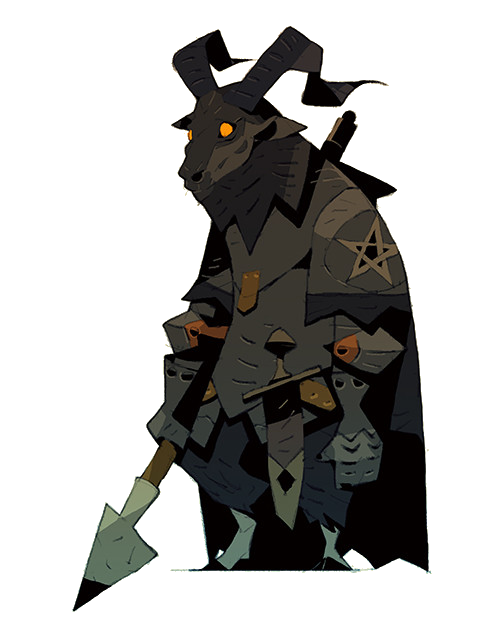
\includegraphics[width=0.47\textwidth]{04kins/img/11gat_knight.png}
\end{figure}

\newpage

\subsubsection{Noves Gat}
    Acclimated to the highest mountains and deepest ravines, cliff gats are the most common of the horned kin.
    Builders of the immense gat city-states, it's very rare to see a cliff gat not actively pursuing their craft.

    \subparagraph{Ability Score Increase} Your time spent in civilization has given you a profound common sense and a general grasp on almost any subject.
    Your Intelligence score is increased by 1.

    \subparagraph{Gat Toughness} Your hit point maximum increases by 1, and it increases by 1 every time you gain a level.

    \subparagraph{Expert Craftsgatship} Noves gats are renowned worldwide for their crafts, and even the untrained eye can recognize an item made by one.
    You are an expert with the artisan's tools associated to your Craftsgatship trait.

    The value of the item you produce in a strange mood is increased to 250,000 GP.
    If you make a weapon, armor, or similar item, it is a +3 item.
    Additionally, you must roll your Strange Mood wisdom saving throw twice at the beginning of every month.

\subsubsection{Bughna Gat}
    In the year 102 AS, the army of healing invaded Ctereth's dwellings and plundered a great haul of qualars.
    These restored the minds of many gats, who became known as the bughna gats.
    % While their minds were recovered, the habits they learned as lost ones have never truly been abandoned.

    Bughna gats feel constrained in cities, and tend to abandon city-states at a young age, freely exploring the outside world.
    % Despite their nature, gats are never truly free of their sense of community.
    Bughna gats tend to travel in packs comprised by varied kins and ethnic groups.

    \subparagraph{Ability Score Increase} Your balance and ability to walk on the steepest of hills is unmatched, and your Dexterity score is increased by 1.

    \subparagraph{Fleet of Foot} Your base walking speed increases by 2 meters.

    \subparagraph{See Them Coming} You have advantage on initiative rolls while in plains, grasslands, and any other open natural environment.

\subsubsection{Treb Gat}
    While many of the gat lost ones were recovered, most of those who wandered off to the dead sea could never be found due to the toxic mist.
    % Here they became the Treb Gat, and eventually acquired qualar back via unknown means.
    These gats are far removed from their calm origins, having to survive the harsh and hostile environment.
    Treb gats have large and muscular bodies, large horns, and dirty, patchy hair.

    \subparagraph{Ability Score Increase} Your restlessness knows no bounds.
    Your Strength score is increased by 1.

    \subparagraph{Size} Treb gats tend to be much larger than their common brethren, measuring between 160 and 200 cm and weighting between 90 and 120 kg.
    Your size is still medium.

    \subparagraph{Uncanny Brutality} While in combat, you are absorbed by a primal rage.
    You have disadvantage on any attacks made with finesse, martial weapons without the heavy property, and ranged weapons.

    \subparagraph{Hammering Horns} You are never unarmed.
    The damage die of your horns is increased to a d6.

    \subparagraph{Savage Attacks} When you score a critical hit with a melee weapon attack, you can roll one of the weapon's damage die one additional time and add it to the extra damage of the critical hit.

    \subparagraph{Fell Mood} When you are struck by a strange mood, the need to craft an exquisite artifact is replaced by an unrelenting urge to kill.
    You have to choose your prey from either a renowned hero, an ancient being, or a forgotten beast.

    After the deed is done, you can craft a disquieting artifact from the creature's remains, following the normal rules of a strange mood.
    All the other conditions of the trait remain the same.%, replacing the need to gather materials with the insatiable craving to hunt said creature.

\begin{figure}[!b]
    \centering
    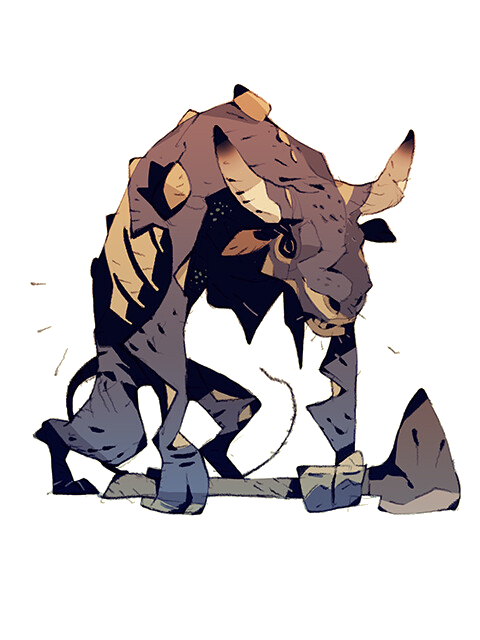
\includegraphics[width=0.48\textwidth]{04kins/img/11gat_treb.png}
\end{figure}

\newpage

% !TEX root = ../main.tex
\section{Winged Kin} \label{kin::ird}
\DndDropCapLine{Y}{es, sure, you can create a machine to}
\textit{glide.
You can even ride a creature to stay aloft.
But you will never truly fly.
No kin can tame the sky with such grace as the irds.
Trust me, if they weren't so humble as to live among us, constrained to the ground, we'd be building temples to venerate their graciousness.}

\hspace*{\fill} --- Josiah, priest from the church of Rhekesh.

Sequestered in high mountains, deep jungles, and hot deserts, the irds, sisz rlue, or winged kin are known to survive some of the harshest environments all around Yuadrem.

\subsection*{Beak and Feather}
    From below, irds look much like large birds.
    Only when they descend to roost or walk in the ground does their humanoid appearance reveal itself.
    Standing upright, an ird might reach 2 meters tall.
    They have long, narrow legs that taper to sharp talons.

    Feathers cover their bodies, with their plumage typically reflecting the environment they develop in.
    Their heads complete the avian appearance, being that of a parrot, hawk, or vulture.
    Irds' arms have very long feathers, which allow them to fly with ease.
    The three subraces of the irds are very distinct from each other.
    This is due to the fact that they were created by three different ets, all in pursuit of a same goal, yet for different environments.

    The winged kin are the only gendered species created by the tall kin.
    Some time after reproduction, a female will lay one to three eggs and the couple will refrain from contact with others in their tribe, becoming extremely protective of their children until they reach maturity.

\subsection*{Sky Wardens}
    Nowhere are the irds more comfortable than in the sky.
    They can spend hours in the air, and some go as long as days, locking their wings in place and letting the thermals hold them aloft.
    In battle, they prove dynamic and acrobatic fliers, moving with remarkable speed and grace, diving to lash opponents with weapons or talons before turning and flying away.

    Once airborne, an ird leaves the sky with reluctance.
    They sometimes forget or ignore vertical distances, and they have nothing but pity for those earthbound kins forced to live and toil constrained to the ground.

    The ird are a tribal species, and its rare for a tribe to hold more than a hundred irds at once.
    The only exceptions to this rule are the Krudzal and Kaldrathal, both large countries in the northern reaches of Yuadrem.
    They are welcoming to traders and visitors in general, but generally don't allow members from other kins to be permanent residents within their territory, and frown upon guests who overstay their welcome.

    Once tribes of irds settle in an area, they share a hunting territory that extends across an area up to 150 km on a side, with each tribe hunting in the lands nearest to their colony, ranging farther should game become scarce.
    A typical colony consists of one large, open-roofed nest made of woven vines.
    The eldest acts as leader with the support of a shaman.

\subsection*{Avian Mannerisms}
    The resemblance of ird to birds isn't limited to physical features.
    Irds display many of the same mannerisms as ordinary birds.
    They are fastidious about their plumage, frequently tending their feathers, cleaning and scratching away any tiny passengers they might have picked up.
    When they deign to descend from the sky, they often do so near pools where they can catch fish and bathe themselves.
    Even when perched on a high branch or at rest in their mountaintop homes, they appear alert, with eyes moving and bodies ready to take flight.

    Many winged kin punctuate their speech with chirps, sounds they use to convey emphasis and to shade meaning.
    An ird might become frustrated with people who fail to pick up on the nuances; an ird's threat might be taken as a jest and vice versa.
    Confinement terrifies the winged kin.
    To be imprisoned by the cold, unyielding earth is a torment few ird can withstand.

\subsection*{Innate Curiosity}
    Irds are naturally curious which, summed with their freedom of movement, leads to them being the ideal explorers and adventurers.
    They use their large wings to travel to almost any place in the entirety of Yuadrem, and as such they've become a common sight in all its reaches.
    Outside of their tribes, irds do enjoy living within other civilizations, and its rare to see a city or large settlement without at least one ird inhabitant.

    % Winged kin tribes are accepting of their members leaving for indefinite amounts of time, and this is even encouraged in many communities.
    % In fact, the population of a tribe is ever-changing, with the only constants being the eldest members and the shaman.
    % This means that neighboring tribes have strong and healthy relations, each coming to aid the ones in need without question.
    % Another consequence of their tendency to travel is the versatility of ird artisans, who integrate techniques from all around Yuadrem into their craft.

\subsection*{Ird Names}
    Ird names separate into two main categories.
    The first resemble their original language, Harualish, and include clicks, trills, and whistles to the point that other kins have a difficult time pronouncing them.
    When interacting with other races, they may use nicknames gained from people they meet or shortened forms of their full names.

    On the other hands, irds from Krudzal, Kaldrathal, and other civilized lands tend to speak Shanise.
    Shanise is a language formed from the interaction of Harualish-speaking irds and Avshenese-speaking gats in the north.

    An ird last name is usually simply ``son/daughter of'' followed by one of their parent's name.
    Most irds admire their parents, and wear their last names with pride.

    \paragraph{Harualish Ird Names}
    Aera, Aial, Aur, Deekek, Errk, Heehk, Ikki, Kleeck, Oorr, Ouss, Quaf, Quierk, Salleek, Urreek, Zeed.

    \paragraph{Male Shanise Ird Names}
    Aden, Azat, Daneal, Dirkir, Eastean, Goker, Idrahin, Jakod, Jaldor, Jasin, Kuneit, Lutdzu, Nuretin, Nutlar, Rezat, Semir, Shasar, Tajik, Tenel, Tshasin, Unut.

    \paragraph{Female Shanise Ird Names}
    Aise, Asutshan, De\~na, Dilsad, Dorun, Drinja, Eda, Gudlag, Gulden, Hazal, Iris, Katrin, Kisnet, Naina, Nerhe, Sehil, Selna, Sher, Solveag, Tedziye, Zainej.

\subsection*{Traits}
    Your ird character has access to different abilities common to all subraces:

    \subparagraph{Ability Score Increase} Your Dexterity score increases by 1, and your Wisdom score increases by 1.

    \subparagraph{Age} Ird reach maturity by age 14, and don't usually live much longer than 150 years.

    \subparagraph{Alignment} Ird have an inclination towards the red tide, which is supported by their adventurous lifestyle.

    \subparagraph{Size} Ird are tall, and range from 1.70 to 2 meters.
    They have thin bodies and hollow bones, weighing between 40 and 50 kilograms.
    Your size is medium.

    \subparagraph{Speed} You have a walking speed of 5 meters, and a flying speed of 10 meters.
    To fly, you can't wear medium or heavy armor, carry heavy weapons, wield a shield or be encumbered.
    Since you flap your arms to fly, you cannot use them to attack while flying.
    You can use your versatile talons to hold and use simple weapons or spellcasting foci.

    If you are hit while flying, roll a Concentration check.
    You have disadvantage on this check if you have a roof above you.
    On a failure, you fall to the ground at a rate of 100 meters per round, taking falling damage when hitting the ground.
    If you haven't landed at the beginning of your next turn, you can continue flying normally, albeit 100 meters below where you were before.

    \subparagraph{Graceful Landing} Your years of living at great heights have taught you how to fall more gracefully.
    You reduce the damage die for fall damage from a d6 to a d4, and you do not fall prone after taking falling damage, unless you are unconscious.

    \subparagraph{Keen Senses} You are competent in the Perception skill.

\subsubsection{Qulbaba Ird}
    Many irds can be found living in isolated tribes inside the jungles of Yuadrem.
    In the east they live in Harual, and in the west in the Jenkashian empire.
    Qulbaba ird have a face resembling that of a parrot, and their feathers' coloration depends on their gender.
    Males usually have very brightly colored feathers, showing any combination of colors.
    Females mostly have dull gray, brown, and dark green feathers, aiding their ability to hide in the jungle.

    \subparagraph{Ability Score Increase} Your time gliding between branches and vines has augmented your flying capacity.
    Your Dexterity score increases by 1.

    \subparagraph{Bright Coloration} As a male, you are competent in the Performance skill.
    Additionally, you have advantage on Charisma (Intimidation) checks made against creatures with an Intelligence score of 5 or less.

    \subparagraph{Dark Feathers} As a female, you have advantage in Dexterity (Stealth) checks made in dim or dark light or in heavily forested areas.

    \subparagraph{Strong Talons} You are competent with unarmed strikes, which deal 1d4 plus your Dexterity modifier as slashing damage on a hit.
    Additionally, you have advantage of Strength (Athletics) checks made to climb any surface your talons could reasonably grip.

    \subparagraph{Language} You know how to speak, read, and write Qualinese and one additional language of your choice.

\begin{figure}[!b]
    \centering
    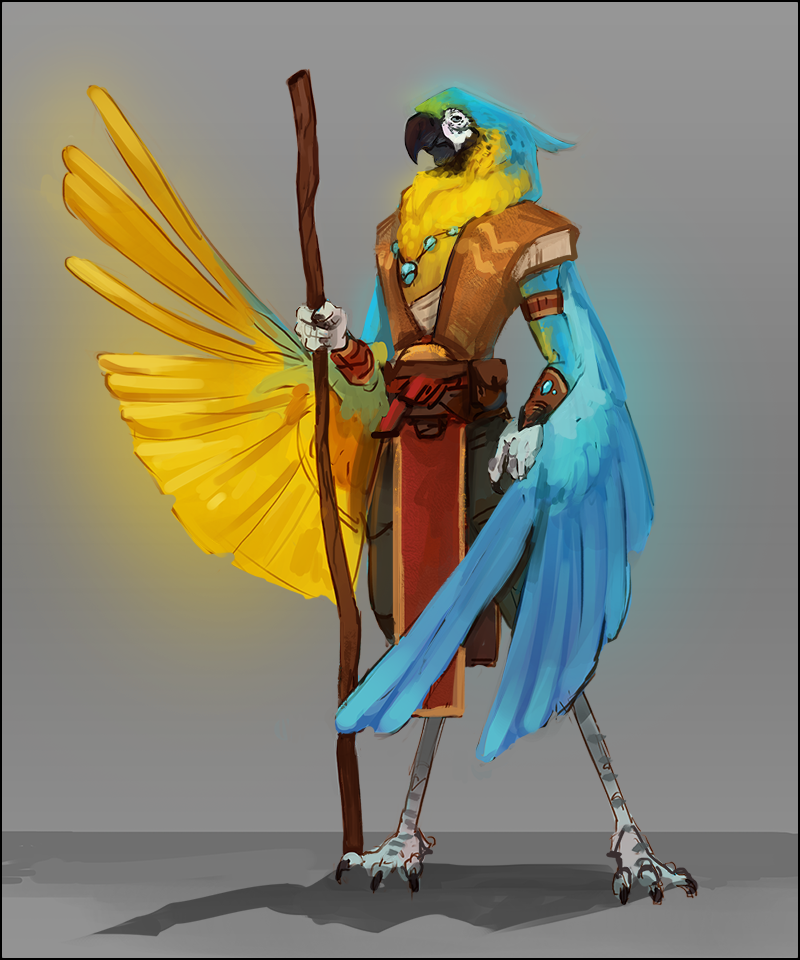
\includegraphics[width=0.48\textwidth]{04kins/img/12ird_qulbaba.png}
\end{figure}

\subsubsection{Thulkraka Ird}
    Unlike their brethren, the Thulkraka tribes that settled on the many mountaintops of Yuadrem live their lives mostly constrained to the ground, and are only able to fly when the harsh mountain weather allows it.
    They are thus bulkier than the average ird, and commonly are clumsy fliers due to their lack of experience.
    Their faces are similar to that of hawks, and their feathers' coloration is bleak and cold, usually sporting white, gray, light blue, and brown colors.

    \subparagraph{Ability Score Increase} Isolated from other races, you have been able to take the time to truly appreciate the calmness of the mountains.
    Your Wisdom score is increased by 1.

    \subparagraph{Bulky Frame} Your flying speed is reduced to 7 meters, but you can fly while carrying heavy weapons and/or wearing medium armor.

    \subparagraph{Mountain Born} You're acclimated to altitudes up to 6,000 meters.
    You're also naturally adapted to cold climates.

    \subparagraph{Thulkrakan Descent} You are competent with smith's tools, as is tradition amongst your people.

    \subparagraph{Language} You know how to speak, read, and write Shanise and one additional language of your choice.

\begin{figure}[!t]
    \centering
    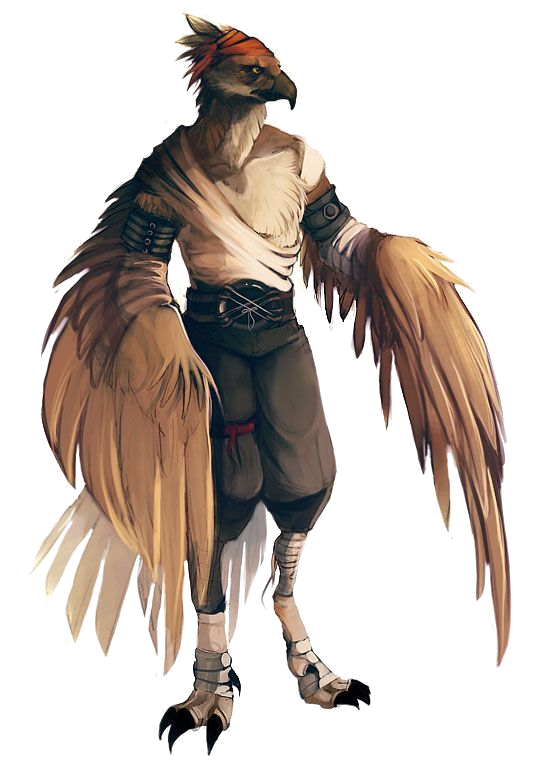
\includegraphics[width=0.47\textwidth]{04kins/img/12ird_thulkraka.png}
\end{figure}

\subsubsection{Dratl Ird}
    Irds from the Dratl houses are known as ruthless ruffians, and are pariahs to the other winged kin subspecies.
    They are known for constantly harassing the other ird tribes, as well as any who approach their territory.
    The are collectively banned from entering any tribe from the other subspecies, and are usually unwelcome in towns and cities due to their bad reputation.

    Nowadays, Dratl houses are scattered around the Zoedrem desert, mostly unorganized.
    These are the remnants of the once great empire of Hulnar, disbanded in 591 AS.
    Despite their lost grandness, they are still feared by the common people, and continue to fiercely protect their hunting grounds.

    A Dratl ird's beak resembles that of a vulture, and their feathers are generally black, white, and red.
    As a dratl ird grows up, their irises become noticeably white, while the sclera surrounding them turn into a bright red color.

    \subparagraph{Ability Score Increase} Your time surviving in the harsh climate of the desert has given you an increased robustness.
    Your Constitution score is increased by 1.

    \subparagraph{Wing Flap} When you use the disengage action, you can choose to use another action to propel yourself upward a distance equal to half your flying speed.

    \subparagraph{Bone Breaker} While flying, you can attempt to attack a creature with an eviscerating attack.
    Using two actions, you can swoop down up to your flying speed towards a creature you can see, and make a melee weapon attack roll against it.
    If the attack hits, it's a critical hit.
    The attack is tiring, and you can use this trait only once per combat encounter.
    % You can use this trait once per combat encounter.

    \subparagraph{Language} You know how to speak, read, and write Zsekian and one additional language of your choice.

% \begin{figure}[!b]
%     \centering
%     \includegraphics[width=0.47\textwidth]{04kins/img/12ird_dratl.png}
% \end{figure}

\newpage

\subsection*{Ird Feats}
    \begin{DndTable}[width=\linewidth, header=Ird Feats]{ll}
        \textbf{Kin or Subrace} & \textbf{Feat} \\
        Ird           & \textbf{Aerial Defense} (page \pageref{feat::aerialdefense})              \\
        Ird           & \textbf{Deadly Grip} (page \pageref{feat::deadlygrip})                    \\
        Ird           & \textbf{Graceful Pass} (page \pageref{feat::gracefulpass})                \\
        Ird           & \textbf{Nimble Step} (page \pageref{feat::nimblestep})                    \\
        Ird           & \textbf{Perfect Landing} (page \pageref{feat::perfectlanding})            \\
        Ird           & \textbf{Songbird} (page \pageref{feat::songbird})                         \\
        Ird           & \textbf{Wing-Assisted Running} (page \pageref{feat::wingassistedrunning}) \\
        Qulbaba Ird   & \textbf{Forest Defender} (page \pageref{feat::forestdefender})            \\
        Qulbaba Ird   & \textbf{Keenest Senses} (page \pageref{feat::keenestsenses})              \\
        Qulbaba Ird   & \textbf{Woodland Hunter} (page \pageref{feat::woodlandhunter})            \\
        Thulkraka Ird & \textbf{Giant Slayer} (page \pageref{feat::giantslayer})                  \\
        Thulkraka Ird & \textbf{Mountain Born} (page \pageref{feat::mountainborn})                \\
        Thulkraka Ird & \textbf{Thulkraka Steel} (page \pageref{feat::thulkrakasteel})            \\
        Dratl Ird     & \textbf{Deadly Precision} (page \pageref{feat::deadlyprecision})          \\
        Dratl Ird     & \textbf{Patient} (page \pageref{feat::patient})                           \\
        Dratl Ird     & \textbf{Savage Attacks} (page \pageref{feat::savageattacks})
    \end{DndTable}

    \subsubsection{Aerial Defense (2 FP)} \label{feat::aerialdefense}
        Creatures who attack you while you're falling, flying, gliding, or jumping have disadvantage on their attack roll.
        \paragraph{Requirements} Ird kin.
    \subsubsection{Deadly Grip} \label{feat::deadlygrip}
        While flying, you have advantage on Grapple checks made with your talons.
        \paragraph{Requirements} Ird kin.
    \subsubsection{Deadly Precision (2 FP)} \label{feat::deadlyprecision}
        Whenever you have advantage on an attack roll using Dexterity, Intelligence, Wisdom, or Charisma, you can reroll one of the dice once.
        Additionally, you learn the \textbf{Aim} action (see page \pageref{act::aim}).
        \paragraph{Requirements} Dratl Ird or Sunstruck Oth subrace.
    \subsubsection{Forest Defender} \label{feat::forestdefender}
        You have received martial training to fight among the branches, and are extremely dangerous to climbing opponents.
        You know the \textbf{Push} action (See page \pageref{act::push}), and the target rolls the saving throw with disadvantage if you climbed, glided, or flew at least 2 meters this turn.
        \paragraph{Requirements} Qulbaba Ird or Marset kin.
    \subsubsection{Giant Slayer (2 FP)} \label{feat::giantslayer}
        An apprentice of the giant slayers from the north, your skill with heavy weapons is unparalleled.
        You gain a +2 bonus to attack rolls made with heavy weapons, and learn the \textbf{Reckless Attack} action (see page \pageref{act::recklessattack}).
        \paragraph{Requirements} Thulkraka ird subrace.
    \subsubsection{Graceful Pass} \label{feat::gracefulpass}
        Using your wings to aid your movement, difficult terrain doesn't cost you extra movement.
        \paragraph{Requirements} Ird or Oth kin.
    \subsubsection{Keenest Senses (2 FP)} \label{feat::keenestsenses}
        You increase your proficiency level with Insight, Investigation, or Perception from Expert to Legendary, increasing your proficiency bonus with the skill to +12.
        \paragraph{Requirements} Qulbaba Ird or Boggart subrace.
    \subsubsection{Nimble Step} \label{feat::nimblestep}
        Opportunity attacks made against you are rolled with disadvantage.
        \paragraph{Requirements} Ird Kin or Gale Zaloth subrace.
    \subsubsection{Patient} \label{feat::patient}
        When you react with a readied action, you have advantage on the first die roll you make as part of that action.
        \paragraph{Requirements} Dratl Ird subrace.
    \subsubsection{Perfect Landing} \label{feat::perfectlanding}
        Furthering your natural falling skills, you are trained to handle any fall with ease.
        As long as you are conscious and can freely use your wings, you are immune to fall damage.
        \paragraph{Requirements} Ird kin.
    \subsubsection{Savage Attacks} \label{feat::savageattacks}
        When you score a critical hit with a melee weapon attack or unarmed strike, you can roll one of the weapon's damage dice one additional time and add it to the extra damage of the critical hit.
        \paragraph{Requirements} Cursed Uman or Dratl Ird subrace.
    \subsubsection{Songbird} \label{feat::songbird}
        Every so often, you can demonstrate the innate power of your Charisma.
        You may cast the charm person spell (see page \pageref{spell::charmperson}) a number of times equal to your Charisma modifier (Minimum of one) per short rest.
        This spell does not require any somatic components to cast.

        The DC of this spell is equal to 10 + your Charisma modifier, but you can increase this by 2 twice by taking this feat again a second and third time.

        Additionally, you have advantage in any Charisma (Performance) check that involves whistling.
        \paragraph{Requirements} Ird kin.
    \subsubsection{Thulkraka Steel} \label{feat::thulkrakasteel}
        You are specially skilled with a set of smith's tools.
        You can craft any metal item for half the normal cost.

        Additionally, if you have access to a forge at an altitude of at least 3,000 meters, you can use the quench-hardening technique unique to your people and craft the item for a quarter its normal cost.
        \paragraph{Requirements} Thulkraka Ird subrace.
    \subsubsection{Wing-Assisted Running} \label{feat::wingassistedrunning}
        You increase your base walking speed by 1 meter.
        Additionally, you gain a climbing speed equal to half your flying speed.
        \paragraph{Requirements} Ird kin.
    \subsubsection{Woodland Hunter} \label{feat::woodlandhunter}
        Your accuracy allows you to treat three-quarters cover as half cover and half cover as no cover.
        \paragraph{Requirements} Qulbaba Ird or Gannagian Hunter subrace.

\newpage~\newpage

% !TEX root = ../main.tex
\section{Archer Kin} \label{kin::marset}
\DndDropCapLine{W}{hile traversing the jungle, be very}
\textit{conscious of your surroundings.
If you stumble upon fiber nests in the trees.
If you hear childlike voices screaming.
Run.
Run as fast as you can.}

\hspace*{\fill} --- Hedwyn's guide to the Chirping Wilds.

The archer kin are a species that resemble large marmosets, barely reaching 90 cm of height.
They share the brown coloration, white ears, and striped tail.
They are small creatures that inhabit the rivers, forests, and jungles of Yuadrem.

They are also known as marsets, or yuathe tle'thal rlue in Jantherlin.
Apart from their size, the other difference from marmosets is their back, which is protected by elongated, pointed quills, used as arrows.

Marsets are an asexual species able to lay eggs at necessity via a ritual after reaching maturity, only limited by the amount of dwellings and social constraints.

\subsection*{Misleading Appearance}
    Marsets don't seem terribly intimidating at first glance.
    They however have an unusual defense mechanism for driving away threats, which includes any unfortunate creature that disturbs their large arboreal colonies.

    Each marset grows specialized quills from their back, with a smooth tip and a base with four flanges, like the fletching of an arrow.
    In additional to making the marsets quite painful to grab, these quills are used as projectiles.

    The little creatures construct their own bows, stripping bark from bendy twigs with their teeth to create the limbs, and harvesting spiderweb for the string.
    The strands are rubbed together with sand, which is done to thicken the bowstring and reduce stickiness in the middle, creating a sophisticated weapon to launch quills at unlucky foes.

    For shorter range, marsets also use hollow reeds to blow their quills as darts.
    It's common for the smarter marsets to apply manure or poison to their arrows and darts, improving their deadliness.

\begin{figure}[!b]
    \centering
    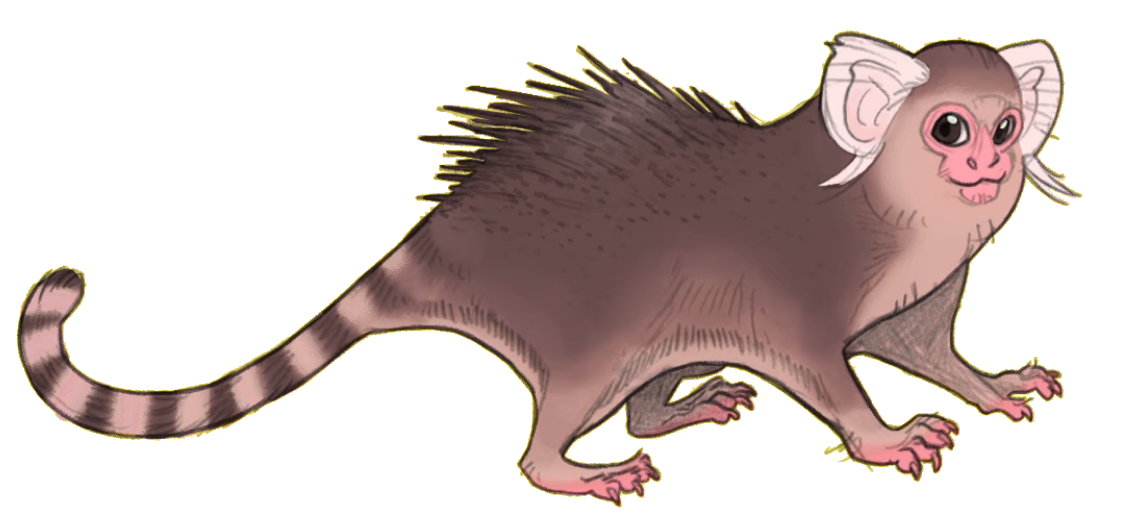
\includegraphics[width=0.48\textwidth]{04kins/img/13marset_brown.png}
\end{figure}

\subsection*{Arboreal Colonies}
    The colonies that the marsets protect are just as complex as their weapons.
    The structures are created from weaving grass and plant fibres around tree branches to create interconnected chambers.

    A single colony can have up to 100 rooms and even more individuals living in it.
    Rooms are assigned a specific function, and are passed down through related members of the colony.

    Nursery rooms are where marsets lay their eggs, which they hatch into fluffy yellow infants.
    Bedrooms are where the adults sleep.
    Storage rooms are where food and various items are stockpiled.

    In farming rooms they deposit a mixture of tough chewed leaves and bark, which then grows mushrooms.
    The little marsets use these rooms to turn otherwise inedible foraged material into something tender and tasty.

    While most marsets can be found in these colonies, some choose to live in cities and towns from other civilizations.
    Here, they usually build interconnected rooms in trees, creating microcosms of the larger colonies.
    Despite their fierceness in their natural environment, marsets are generally regarded as friendly creatures when encountered in urban settings.

\begin{figure}[!t]
    \centering
    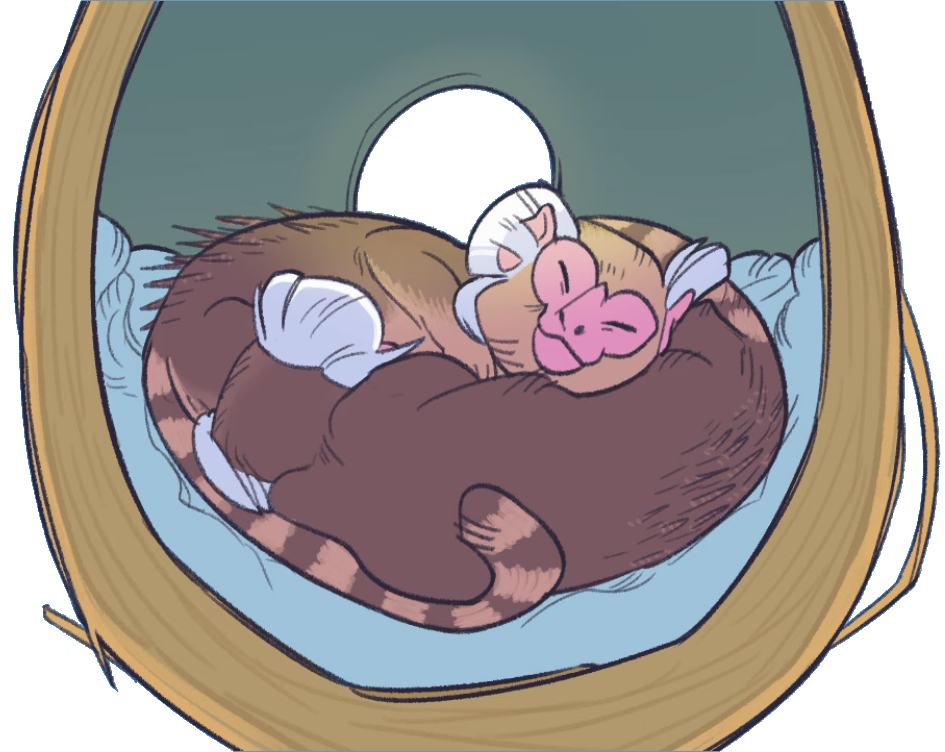
\includegraphics[width=0.48\textwidth]{04kins/img/13marset_room.png}
\end{figure}

\subsection*{Repetitive Language}
    Marsets hatch from their eggs already able to speak a strange repetitive language, which is entirely regular and does not evolve.
    This language --- known as Babazano --- can be spoken in one of two ways: soundlessly, with the communication happening through lip reading, or screamed as loud as possible, with no middle ground.
    Despite this, a marset can learn other languages and not constantly scream at the top of their lungs, but they do tend to be loud speakers.

    Babazano has only ten consonants.
    All verbs use a single consonant as their root, so there's only ten verbs.
    By repeating syllables they create new meanings, which makes their language very difficult to understand by the other kins, but for these little creatures it's no issue at all.
    They hear or lip-read a word and instinctively know which one it is.

\subsection*{Exploring Opportunities}
    Marsets don't usually set out on the adventurer's path for leisure, but rather out of necessity.
    They will only leave their colonies to defend their communities or support their friends.
    Only very few will set out to explore the wide world.
    % For them, adventuring is less a career than an opportunity and more of a necessity.

\begin{figure}[!t]
    \centering
    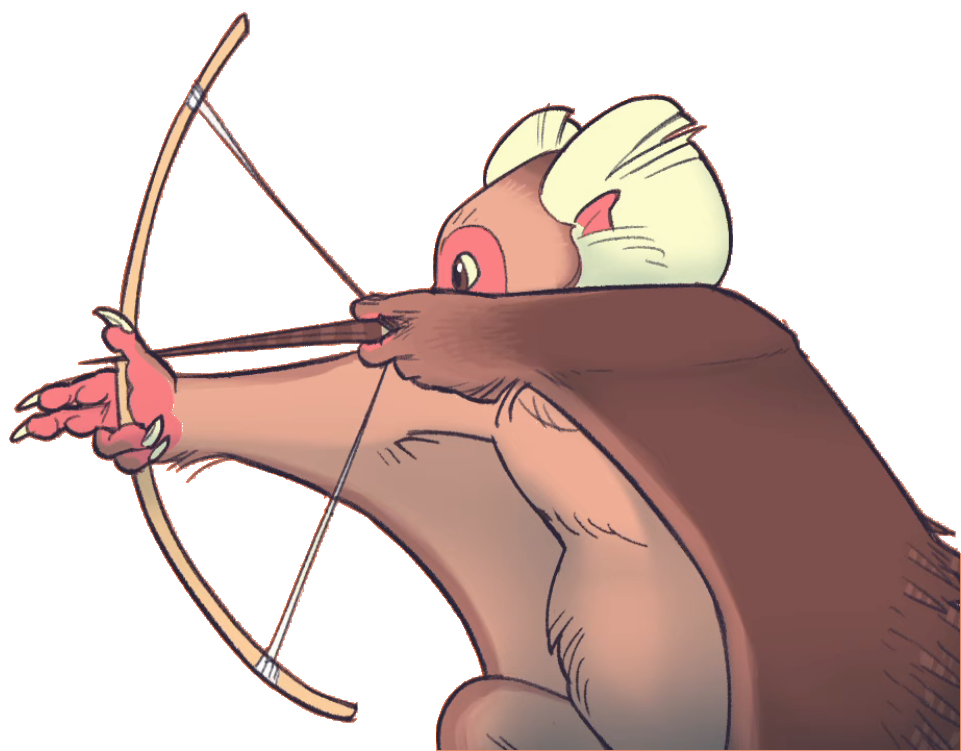
\includegraphics[width=0.48\textwidth]{04kins/img/13marset_bow.png}
\end{figure}

\subsection*{Marset Names}
    Marsets assign names to each other based on distinctive features and accomplishment.
    An individual marset will wear many names during their childhood, and when they settle on one is when they reach adulthood.
    Due to the peculiarity of Babazano, it is a common for the other kins to call them by simple monikers, practice that the marsets despise.
    % Most marsets don't particularly like this, and are very reluctant to accept a nickname given to them.

    \paragraph{Names}
    Do Anana, Do Baba, Do Badada, Do Ebebebebe, Do Ezeze, Do Nono, Do Odododo, Do Uvu, Do Veve, Do Vovovo.

\subsection*{Traits}
    Your marset character has a range of abilities based on its nature and community lifestyle.

    \subparagraph{Ability Score Increase} Your Charisma score is increased by 2, and your Dexterity score is increased by 1.

    \subparagraph{Age} Marsets has a short lifespan, reaching maturity by age 4 and not living much more than 50 years.

    \subparagraph{Alignment} Marsets have a tendency towards helping others, specially in their communities, and are inclined towards the gold tide.

    \subparagraph{Size} Marsets range from 75 to 90 cm.
    They usually have a slender and agile frame, weighing around 20 kg.
    Your size is small.

    \subparagraph{Speed} Your base walking speed is 9 meters, and you have a climbing speed of 9 meters.

    \subparagraph{Glider} You have loose flaps of furry skin between your arms and legs, which allow you to glide short distances at a speed of 9 meters per turn, as long as you are not wearing heavy armor.
    You fall at a rate of 6 meters per turn while gliding, and suffer no falling damage on landing.

    \subparagraph{Sneaky Nature} You have advantage on stealth checks in heavily forested areas.

    \subparagraph{Natural Weapons} You are proficient with shortbows and blowguns, and can use your own quills as arrows or cut them to be used as darts.
    Every day you can gather up to 10 quills from your back to be used in this fashion.

    \subparagraph{Community lifestyle} Despite their loudness, marsets can be very compelling talkers.
    You are competent in the Persuasion skill.

    \subparagraph{Languages} You can speak Babazano from birth, and can lip-read the language.
    You are also able to read and write Leafrunes, a special writing system designed to communicate simple messages to others of your kin.
    Additionally, you know how to speak a language of your choice, but you don't know how to read or write it.

\begin{figure}[!b]
    \centering
    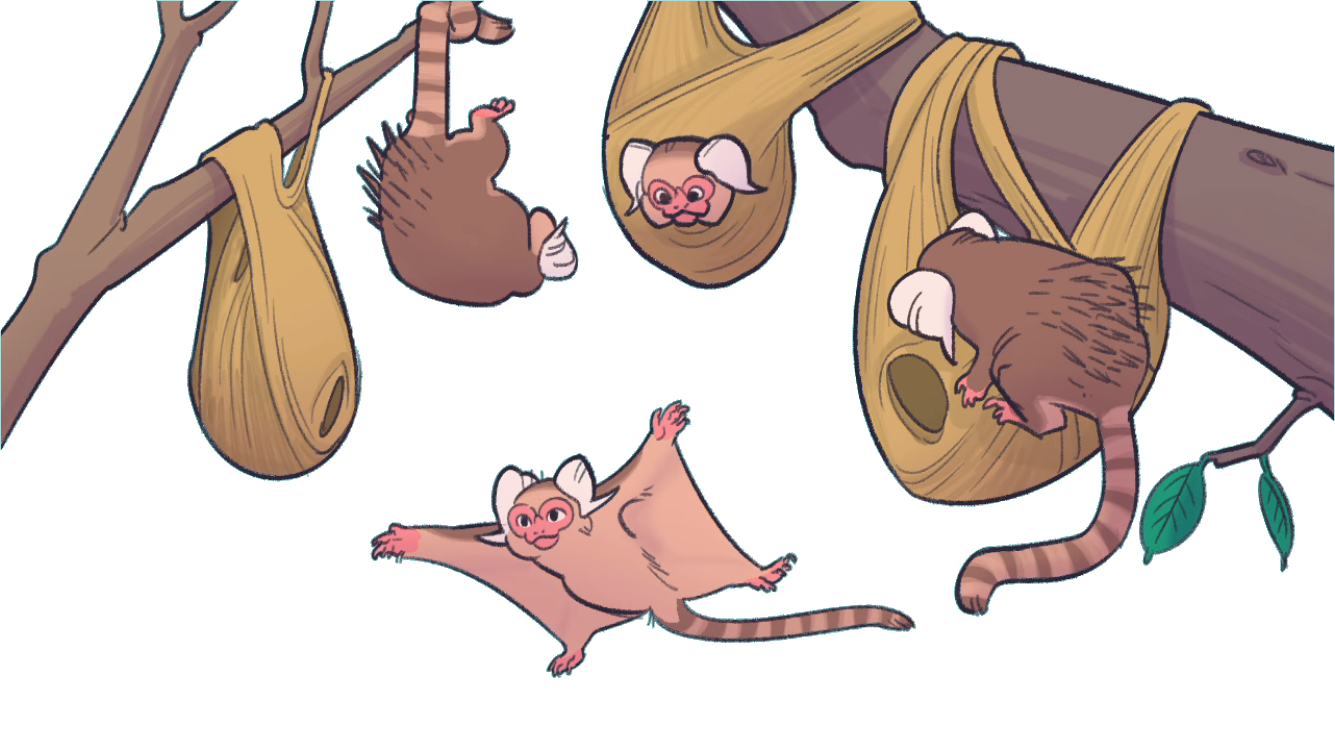
\includegraphics[width=0.48\textwidth]{04kins/img/13marset_colony.png}
\end{figure}

\newpage

% !TEX root = ../main.tex
\section{Dust Kin} \label{kin::oth}
\DndDropCapLine{T}{he light beckons, and you follow.}
\textit{As the light lead you once, now you are guided by enlightenment.
With each hidden truth you uncover, you learn more of what the world is, and how to secure your place in it.
Secrets are your power and your currency.
Seek them out, and guard them well.}

\hspace*{\fill} --- Ancient Moonborn saying.

Moody and perplexing.
Isolated and elegant.
Tough and passionate.
The ways in which one might describe the dust kin are many.
The dust kin, oths, or szua-tlekeloo rlue are a quiet species with a tendency towards nature and knowledge.
They're a solitary yet intimate creature with a penchant for nature and ritual.

\subsection*{Enigmatic and Uncanny}
    While oths can be see as much as gats or irds around civilized lands, they are far more mysterious and reclusive than the two.
    Often silent, oths have a reputation for being cryptic and thoughtful.
    They tend to follow their intuition on a whim.

    Oths usually travel with a large scroll in their backs made from their own fabric, which they protect with impermeable and resilient guards.
    This scroll is a compendium of knowledge passed down through generations, and they add to it in key moments in their life.

    The dust kin have large, heavy forewings that hang around their humanoid bodies like cloaks, which hide a shorter and more delicate set of hindwings behind them.
    They have two sets of arms, one above the other.
    The upper pair is strong and long, while the lower one is weak, and mostly left for secondary tasks.
    Their feet have three fingers and their arms have four, with one being an opposable thumb.
    They have an insectoid face with antennae and compound eyes.
    Their body is covered in a short, fluffy hair which is usually of a very pale brown color.

\subsection*{Long Tempers}
    Through generational learning, oths are wise and prudent creatures from a very early age.
    Many chase intellectual or mindful pursuits, becoming librarians and philosophers.
    They pontificate on the nature of life and knowledge.
    Most think that the oth are naturally intelligent, and take their opinions with very high regard.

    While most dedicate to cultivating their cognition, some decide to live their lives in adventure.
    They nurture their minds with experience, acquiring knowledge via facing the challenges of the world.

    A common thread throughout the race is that they are slow to anger.
    Regardless of culture, it is instilled in them as early as the larval stage.
    Life is too short to be spent in anger or frustration.

\subsection*{Cycle of Resurrection}
    An oth knows when their natural death approaches, and faces it peacefully.
    When they are near their death, they say their goodbyes and withdraws from civilized society.
    The oth then pilgrimages towards a cavern or secret place they designated during their lifetime.

    On arrival, the oth blocks all but one entrance to this sacred place, and lays ten to twenty eggs in a bed of silk during fall.
    They then spend their time gathering foodstuffs and lining the walls, floor, and roof with silk, providing a safe environment for their descendants to develop in.
    The oth also uses this time to finish writing their compendium of knowledge in their scroll, developing it until its ready to be passed on to their strongest descendant.

    At the last week before the break of summer, the oth closes the last entrance to its sacred place, engulfing it in total darkness.
    And they wait.

    At some point during summer, the eggs hatch for their parent to greet and nourish their newborn larvae.
    They dying oth hands qualars to their progeny, teaching them their language and the way of the world.
    Along with this they pass on the tenets of their culture.
    The parent eats no more than a grain of rice per day, and refrains almost completely from liquids.

    Six months after hatching, the younglings go through the process of pupation, remaining as pupa for a year.
    The parent uses this time to drink an embalming fluid, and mummifies themselves in silk.
    They slowly lose their sentience, peacefully drifting into non-existence.

    After hatching, the oths pay tribute to their now dead parent, and re-seal their cradle.
    The first place they see becomes their parent's final resting place.
    The oths then travel together, forming a small familiar tribe which lasts until they reach maturity.
    While the members of the family may part ways, the bond they share is never truly broken.

\subsection*{Educated by Experience}
    Due to the way the oths spend their youths, they are generally very wise from a very young age, blessed with the knowledge of the previous generations.
    However, it's in an oth's nature to cultivate this wisdom with a contemporary and personal viewpoint of the world.
    It's rare to see an oth not spending much of their youth travelling for knowledge and wisdom.
    % The dust kin is also very concerned about the preservation of nature, and are experts at recording its sights and dwellers in great detail.

\subsection*{Oth Names}
    In oth culture, the parent is assigned the task of naming each of their children in their larval stage.
    These names will often change at the whim of the parent, not becoming official until pupation.
    Their names are often difficult to pronounce by the other kins, and most don't mind being called by a nickname for simplicity.
    The dust kin doesn't use family names, recognizing their relatives by sight alone.

    \paragraph{Names}
    Adz'kt, Andle, Axa, Bixi, Chch, Chith, Daph, Fen'kt, Fl'ka, Fra, G'zigg, Gl'rik, Hadae, Iitus, J'llkx, Kl'il, Lenna, L'kpha, Mlf, N'kakt, Riz, Scelkt, Sud'kx, Thm, Timpth, Zkx.

% \begin{table*}[b]%
%     \begin{DndTable}[width=\linewidth, header=Oth Silk Armor]{lXXXX}
%         \textbf{Armor} & \textbf{AC} & \textbf{DC} & \textbf{Time taken} & \textbf{Cost} \\
%         Silk Armor                & 11 + Dex mod     & 10 & 1 week   &    -    \\
%         Reinforced Silk Armor     & 12 + Dex mod     & 15 & 2 weeks  &   10 GP \\
%         Exquisite Silk Armor (+1) & 12 + Dex mod + 1 & 20 & 1 month  &  100 GP \\
%         Excellent Silk Armor (+2) & 12 + Dex mod + 2 & 20 & 6 months & 1000 GP
%     \end{DndTable}
% \end{table*}

\subsection*{Traits}
    Your oth character has the following set of skills, based on its customs and ancestry.

    \subparagraph{Ability Score Increase} Your Intelligence score increases by 2.

    \subparagraph{Age} An oth will go through three stages of growth: eggs, larvae, and pupa.
    This development takes in total about two years.
    In terms of maturity, they emerge from their pupa as adults, but reach full size at about ten years of age.
    Oths live to be around 80 years old.

    \subparagraph{Alignment} Oth tend to stray from extremes, most often remaining neutral in conflicts as long as there is no direct danger to themselves or those close to them.
    The oths passion for wisdom leads them to the blue tide.

    \subparagraph{Size} Oth typically range from between 135 to just under 180 cm.
    Your size if Medium.
    You are impressively lightweight for your size, weighing around 45 kg.

    \subparagraph{Speed} Your base walking speed it 6 meters.

    \subparagraph{Clumsy Flight} Once per short rest, you can fly with a speed of 4 meters for a number of rounds equal to your Constitution modifier plus 2, with a minimum of 2 rounds.
    You cannot use this feature while you wear heavy armor or carry heavy weapons.

    \subparagraph{Darkvision} Due to your nocturnal heritage you have a good sense of vision in the dark.
    You can see in dim light within 12 meters of you as if it were bright light, and in darkness as if it were dim light.
    You can't discern color in darkness, only shades of gray.

\begin{figure}[!t]
    \centering
    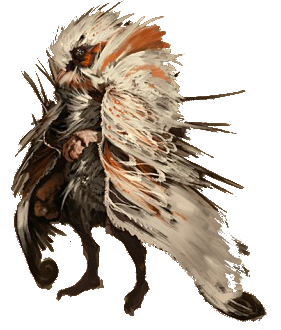
\includegraphics[width=0.48\textwidth]{04kins/img/14oth_white.png}
\end{figure}

    \subparagraph{Four-armed} You have a pair of weaker secondary arms that can be used to hold small objects and perform simple tasks.
    You cannot use these arms to wield weapons or shields and Strength checks using them are made with disadvantage.
    Due to your unique form, armor may need to be specially made, leading to additional costs.

    \subparagraph{Languages} You know how to speak, read, and write Shamabic and one other language of your choice.

\subsubsection{Moonborn}
    The moonborn are the most common of the oth.
    They prefer shady areas, and tend to live their lives in such places.
    They have been properly schooled under the light of Nuagal as oth tradition dictates, and many can be found in darkened libraries during daytime.

    As their name suggests, moonborn have a special affinity for Nuagal, and can even feed off its light.
    They travel at night and hide during the day, and most carry a specially designed tent that blocks all incoming sunlight.

    \subparagraph{Ability Score Increase} Your Wisdom score is increased by 1.

    \subparagraph{Light Sensitivity} Moonborn grow away from the sun.
    You are vulnerable against radiant damage.
    You have disadvantage on attack rolls and Wisdom (Perception) checks that rely on sight when you, the target of your attack, or what you are trying to perceive is under direct sunlight.

    \subparagraph{Sensitive Antennae} Using your specialized antennae, you have advantage on perception checks that rely on smell.

    \subparagraph{Lunar Studies} You are competent in the Religion and History skills.

    \subparagraph{Moon Magic} You know the \textbf{Light} spell (see page \pageref{spell::light}), which you can freely cast.
    When you reach third level, you learn the \textbf{Faerie Fire} spell (see page \pageref{spell::faeriefire}), which you can cast once per day.
    When you reach fifth level, you learn the \textbf{Glitterdust} spell (see page \pageref{spell::glitterdust}), which you can cast once per day.

    Intelligence is your spellcasting modifier for these spells.

\subsubsection{Chu'ash Kin}
    The chu'ash oths are a subculture that differentiate from the rest by their curious and reckless nature.
    Weaker than their siblings, they are born a summer too late, and never get to meet their parent.
    They are instead cared for by their older siblings, and are the younger members of their familiar tribes.

    To most, a chu'ash oth seems perpetually disorganized and distracted, which leads to the belief that they have a lower intelligence to the other of their kin.
    In truth, the chu'ash have a unique perception of the world.
    They are able to interpret information in a unique way, allowing them to see possibilities other cannot.
    Born with an untamed intelligence, the chu'ash oth has an affinity to find the hidden patterns of the world.

    \subparagraph{Ability Score Increase} Your Charisma score is increased by 1.

    \subparagraph{Fated} Whether luck of a guiding presence, you always seem to find your way.
    Once per day you can choose to reroll an attack, skill check, or saving throw.
    You can decide to do this after the roll, but before the outcome of the roll has been determined.

    \subparagraph{Touched} You know the \textbf{Dancing Lights} spell (see page \pageref{spell:dancinglights}), which you can freely cast.
    When you reach third level, you learn the \textbf{Color Spray} spell (see page \pageref{spell:colorspray}), which you can cast once per day.
    When you reach fifth level, you learn the \textbf{Blur} spell (see page \pageref{spell:blur}), which you can cast once per day.

    Charisma is your spellcasting modifier for these spells.

\subsubsection{Sunstruck Oth}
    While most oths follow the circle of resurrection to the letter, there are a few who choose to ignore it.
    They lay their eggs under direct sunlight, and their larvae quickly lose their fragile hindwings.
    Unrepairable, their wings stay atrophied and shriveled thorough their lives.

    These oths are known as the sunstruck, and they've earn a reputation of unpaired hardiness and resilience.
    The clans of Shief and Zmiva cherish this attribute, and consciously molt in lit areas to engender it.

    \subparagraph{Ability Score Increase} Due to your hardiness, your Constitution score is increased by 1.

    \subparagraph{Sunstruck Birth} You lose your \textbf{Clumsy Flight} and \textbf{Darkvision} traits.

    \subparagraph{Photosynthesis} While you need water like any other creature, you don't need to eat to gain sustenance.
    You can choose to instead collect light with your wings via photosynthesis.
    Each day, you must spend two hours with your hindwings exposed to sunlight, or four hours to moonlight to be properly well fed.

    \subparagraph{Sunstruck Resilience} You are competent in the Survival skill.

    \subparagraph{Vertical Takeoff} As an action, you can use your powerful frame and knowledge of thermals to propel yourself upward a distance equal to double your movement speed.
    This technique is used by the Shief scouts to survey the desert around them in search of food or predators.

    \subparagraph{Slow Fall} While useless for flight, your shriveled wings allow you to slow your fall.
    When falling, you can use an action or reaction to lift your wings using your second pair of arms to slow your descent.
    You continue to fall gently at a speed of 6 meters per round, taking no fall damage when you land.
    You cannot use this trait if you are wearing heavy armor or are encumbered.

\subsection*{Oth Feats}
    \begin{DndTable}[width=\linewidth, header=Oth Feats]{ll}
        Oth           & \textbf{Born Grappler} (page \pageref{feat::borngrappler})       \\
        Oth           & \textbf{Graceful Pass} (page \pageref{feat::gracefulpass})       \\
        Oth           & \textbf{Keen Mind} (page \pageref{feat::keenmind})               \\
        Oth           & \textbf{Predenstined} (page \pageref{feat::predenstined})        \\
        Oth           & \textbf{Silent Speech} (page \pageref{feat::silentspeech})       \\
        Oth           & \textbf{Silkspinning} (page \pageref{feat::silkspinning})        \\
        Oth           & \textbf{Third Weapon} (page \pageref{feat::thirdweapon})         \\
        Moonborn Oth  & \textbf{Linguist} (page \pageref{feat::linguist})                \\
        Moonborn Oth  & \textbf{Magic Initiate} (page \pageref{feat::magicinitiate})     \\
        Moonborn Oth  & \textbf{Observant} (page \pageref{feat::observant})              \\
        Chu'ash Oth   & \textbf{Bountiful Luck} (page \pageref{feat::bountifulluck})     \\
        Chu'ash Oth   & \textbf{Fey Touched} (page \pageref{feat::feytouched})           \\
        Chu'ash Oth   & \textbf{Lucky} (page \pageref{feat::lucky})                      \\
        Sunstruck Oth & \textbf{Bone Breaker} (page \pageref{feat::bonebreaker})         \\
        Sunstruck Oth & \textbf{Deadly Precision} (page \pageref{feat::deadlyprecision}) \\
        Sunstruck Oth & \textbf{Sun-powered} (page \pageref{feat::sunpowered})
    \end{DndTable}

    \subsubsection{Bone Breaker} \label{feat::bonebreaker}
        While gliding, you can attempt to attack a creature with an eviscerating attack.
        Using two actions, you can swoop down up to your movement speed towards a creature you can see, and make a melee weapon attack roll against it.
        If the attack hits, it's a critical hit.
        The attack is tiring, and you can use this feat only once per combat encounter.
        \paragraph{Requirements} Sunstruck Oth subrace.
    \subsubsection{Born Grappler} \label{feat::borngrappler}
        You don't need to have a hand free to grapple, using both your extra arms to do so.
        If you do have a free arm, you roll for the grapple check with advantage.
        You cannot use this feat if you are holding something in one or both of your extra arms.
        \paragraph{Requirements} Oth kin.
    \subsubsection{Bountiful Luck (2 FP)} \label{feat::bountifulluck}
        Your people have extraordinary luck, which you have learned to lend to your companions when you see them falter.
        You're not sure how you do it; you just wish it, and it happens.
        Surely a sign of fortune's favor!

        When an ally you can see within 6 meters of you rolls a 1 on the d20 for an attack roll, an ability check, or a saving throw, you can use your reaction to let the ally reroll the die.
        The ally must use the new roll.

        When you use this ability, you can't use your Fated trait before the end of your next turn.
        \paragraph{Requirements} Chu'ash Oth subrace.
    \subsubsection{Fey Touched} \label{feat::feytouched} % TODO. REWORK.
        You learn the misty step (see page \pageref{spell::mistystep}) and one 1st-level spell of your choice.
        The spell must be from the Sympathy doctrine.
        You can cast each of these spells without expending a spell slot.
        Once you cast either of these spells in this way, you can't cast that spell in this way again until you finish a short rest.
        You can also cast these spells using spell slots you have of the appropriate level.
        The spells' spellcasting ability is Intelligence.
        \paragraph{Requirements} Chu'ash Oth subrace.
    \subsubsection{Linguist} \label{feat::linguist}
        You have studied languages and codes, gaining the following benefits:
        \begin{itemize}
            \item You learn a language of your choice.
            \item You can ably create written ciphers.
            Others can't decipher a code you create unless you teach them, they succeed on an Intelligence check (DC equal to 8 + your Intelligence score), or they use magic to decipher it. % TODO: Figure out what spell (probably from Dremshamad) would be able to do this.
        \end{itemize}
        \paragraph{Requirements} Moonborn Oth subrace.
    \subsubsection{Lucky} \label{feat::lucky}
        When you roll a 1 on an attack roll, ability check, or saving throw, you can reroll the die and must use the new roll.
        This doesn't count as a use of the Fated trait.

        You can use this trait a number of times equal to your Charisma modifier (minimum of 1) per short rest.
        \paragraph{Requirements} Tortle kin or Chu'ash Oth subrace.
    \subsubsection{Magic Initiate (2 FP)} \label{feat::magicinitiate} % TODO. REWORK.
        Your learn two cantrips of your choice from one spellcasting doctrine of your choice.
        In addition, choose one 1st-level spell from the same doctrine.
        You learn that spell and can cast it at its lowest level.
        Once you cast it, you must finish a long rest before you can cast it again using this feat.
        Your spellcasting ability for these spells is Intelligence.
        \paragraph{Requirements} Moonborn Oth subrace.
    \subsubsection{Observant} \label{feat::observant}
        You gain a +5 bonus to your passive Wisdom (Perception) and passive Intelligence (Investigation) scores.
        \paragraph{Requirements} Moonborn Oth or Na'anian Tsanek subrace.
    \subsubsection{Predestined} \label{feat::predenstined}
        Once per day you can choose to reroll an attack, skill check, or saving throw.
        You can decide to do this after the roll, but before the outcome of the roll has been determined.
        If you are a Chu'ash oth, consider your Fated trait as one additional use of this feat.

        You can learn this trait 3 times, increasing the number of times you can use this feat per day by one each time.
        On the third time, you gain the ability to use this trait to force an enemy to reroll an attack roll made against you.
        \paragraph{Requirements} Oth kin.
    \subsubsection{Silent Speech} \label{feat::silentspeech}
        You can communicate with other oths, thri-kreen, and other insectoids using Silent Speech.
        This language can only communicate simple ideas, and it does so via a combination of pheromones and thrumming sounds made with antennae.
        \paragraph{Requirements} Oth kin.
    \subsubsection{Silk Spinning} \label{feat::silkspinning}
        Dust kin's silk is known for its beauty and strength, and oth's know how to craft clothes and various items with it.
        Your silk counts as a cloth material, and armor made with it has a +1 bonus to its AC.
        You can produce up to one kg of silk per long rest, which you can store for future use.
        \paragraph{Requirements} Oth kin. At least Competent proficiency with weaver's tools.
    \subsubsection{Sun-powered} \label{feat::sunpowered}
        By reabsorbing your sweat and taking in dew, you do not need to drink water to survive.
        You gain full sustenance when you use your \textbf{Photosynthesis} trait, including both food and water.
        Additionally, you only need to keep your hindwings for one hour exposed to sunlight or two hours exposed to moonlight to be properly well fed.
        \paragraph{Requirements} Sunstruck Oth subrace.
    \subsubsection{Third Weapon (2 FP)} \label{feat::thirdweapon}
        You can use your two extra arms to hold a weapon with the light property.
        You can attack with this weapon as a free action after you make a melee weapon attack, reducing the attack roll by the apropiate multiple attack penalty.
        \paragraph{Requirements} Oth kin.

\begin{figure}[!t]
    \centering
    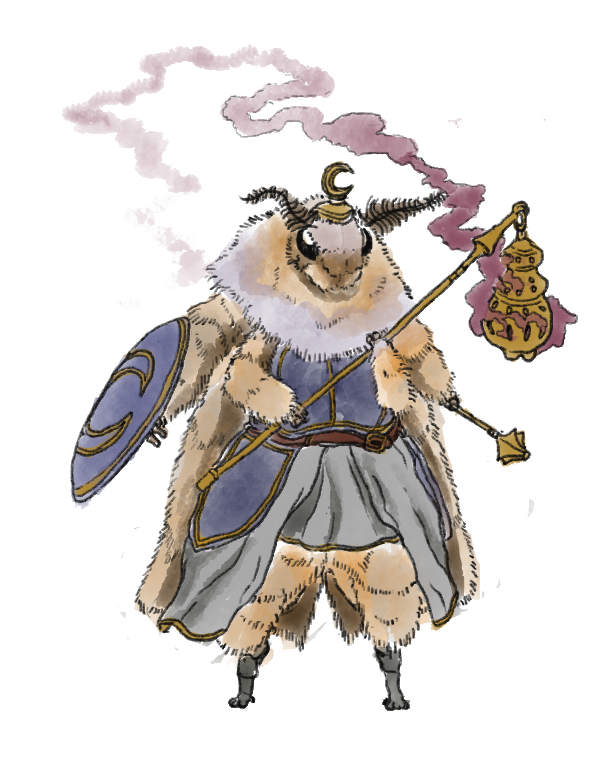
\includegraphics[width=0.48\textwidth]{04kins/img/14oth_cleric.png}
\end{figure}

\subsection*{Oth Spells}
    \DndSpellHeader{Blur \label{spell::blur}}
        {Chu'ash spell}
        {2 action}
        {Self}
        {S (forewings)}
        {Concentration, up to 1 minute}
        You flutter your forewings in a frantic manner, lifting a refracting golden dust around you.
        Your body becomes blurred, shifting and wavering to all who can see you.
        For the duration, any creature has disadvantage on attack rolls against you.
        An attacker is immune to this effect if it doesn't rely on sight, as with blindsight, or can see through illusions, as with truesight.
    \DndSpellHeader{Color Spray \label{spell::colorspray}}
        {Chu'ash spell}
        {2 actions}
        {Self (9-meter cone)}
        {S (hindwings)}
        {1 round}
        A dazzling array of flashing, pale-colored light springs from your hindwings.
        Roll a number of d10s equal to double your level; the total is how many hit points of creatures this spell can effect.
        Creatures in a 9-meter cone originating from you are affected in a ascending order of their current hit points (ignoring unconscious creatures and creatures that can't see).

        Starting with the creature that has the lowest current hit points, each creature affected by this spell is blinded until the end of your next turn.
        Subtract each creature's hit points from the total before moving on to the creature with the next lowest hit points.
        A creature's hit points must be equal to or less than the remaining total for that creature to be affected.
    \DndSpellHeader{Dancing Lights \label{spell::dancinglights}}
        {Chu'ash spell}
        {2 actions}
        {24 meters}
        {M (a firefly or a gram of silver moss)}
        {1 hour}
        You create up to four torch-sized pale blue orbs within range that hover in the air for the duration.
        You can also combine the four lights into one glowing object vaguely resembling a creature of Medium size.
        Each light sheds dim light in a 6-meter radius.

        As a bonus action on your turn, you can move the lights up to 12 meters to a new spot within range.
        A light must be within 4 meters of another light created by this spell, and a light winks out if it exceeds the spell's range.
    \DndSpellHeader{Faerie Fire \label{spell::faeriefire}}
        {Moonborn spell}
        {2 actions}
        {Self}
        {S (forewings)}
        {1 minute}
        You flutter your forewings, spreading a blue dust into the air.
        Each object in a 9-meter radius around you is outlined in a pale blue light.
        Any creature in the area when the spell is cast is also outlined in the light.
        For the duration, objects and affected creatures shed dim light in a 6-meter radius.

        Any attack roll against an affected creature or object has advantage if the attacker can see it, and the affected creature or object can't benefit from being invisible.

        A creature can try to shake off the dust as an action by succeeding on a Dexterity saving throw.
        The dust stops glowing after a minute.
    \DndSpellHeader{Glitterdust \label{spell::glitterdust}}
        {Moonborn spell}
        {2 action}
        {Self}
        {S (hindwings)}
        {1 minute}
        You flutter your hindwings, spreading a white dust into the air.
        A cloud of golden particles covers everyone and everything within a 3-meter radius around you.
        All creatures and objects within the area are covered by the dust, which cannot be removed and continues to sparkle until it fades.

        For the duration, any target covered by the dust has disadvantage on Dexterity (Stealth) checks, and gains no benefit from being invisible.

        Each creature affected by the spell must succeed on a Wisdom saving throw or become blinded for the duration.
        The creature can repeat its saving throw at the end of each of its turns, ending the blindness on a success.
    \DndSpellHeader{Light \label{spell::light}}
        {Moonborn spell}
        {2 actions}
        {Touch}
        {M (a firefly or a gram of silver moss)}
        {1 hour}
        You touch one object that is no larger than 2 meters in any dimension.
        Until the spell ends, the object sheds bright light in a 6-meter radius and dim light for an additional 6 meters.
        The light is of a pale blue color.
        Completely covering the object with something opaque blocks the light.
        The spell ends if you cast it again or dismiss it as an action.

        If you target an object held or worn by a hostile creature, that creature must succeed on a Dexterity saving throw to avoid the spell.

\newpage~\newpage

% !TEX root = ../main.tex
\section{Moss Kin} \label{kin::naenk}
\DndDropCapLine{W}{e thought they were mindless}
\textit{savages, but they know what they're doing.
They ain't hiding from us, they're preparing an attack.
They're studying our movement, figuring out our tactics.
They're hunting us.}

\hspace*{\fill} --- Phokrax, Drejeck expedition leader.

The moss kin, or naenks, are moss creatures that hunt in the dark, warm, and wet jungles of Drejeck.
They hunt for sustenance and to gather fresh corpses.

\subsection*{Short and tangled}
    The naenks are mostly known for their strange reproduction.
    They spawn from the corpses of hunted humanoids exposed to the nanust spores of the great tree Tekatsae.
    The spores grow into moss, merging with the corpse's muscle tissue and flesh.
    After a period of about two months, the corpse rises again, this time in the shape of a naenk.

    The moss kin are a thin race.
    Their height varies considerably, but they usually are slightly smaller than their birth corpse.
    Their bodies mock a humanoid shape, made up by a mix of bone, flesh, vine, and moss.
    They protect their fragile interior with thick layers of flora.

    Naenks typically have a healthy green coloration, but their skin can be of any mix of colors between moldy blue, dark orange, gray, and even white.
    Their eyes are of a white or yellow color, where a thick fluid hides their pupils from the eyes of others.

    Naenks naturally grow leaves and mossy tendrils at the top of their heads that resemble hair, which can be of a black, brown, or yellow color.
    They typically arrange this mock-up of hair in a simple topknot.

    % Due to the duality of their bodies, naenks follow a very particular diet.
    % They needs to regularly consume meat in order to maintain the corpse inside them.
    % They also feed off nutrients from the soil to feed the vines and plants that surround this corpse.

\subsection*{Tribal Communities}
    % A naenk also assists their communication with rhythmic tapping on their body and using a complex system of gestures.
    % Apart from these, they can also speak telepathically when close to tsaneks or sovereigns, aiding their communication.

    Naenks are organized in tribal units called bands.
    Each band is lead by the strongest naenk, the chief, who commands alongside a tsanek shaman.
    Naenk chiefs bear special spores that can be used to infect beasts in a manner similar to the Tekatsae tree.
    They spawn a bestial moss creature known as nuen with this spores, who acts as a pet or mount to the chief.
    When a naenk travels alone, it is usual for them to also grow these spores as well.

    Naenks build and craft very little.
    Their gear is simply what they loot, and they build simple structures by imitation.

    Due to their odd appearance and homicidal reproduction, naenks are seen as something to fear.
    They however are very bold, yet fear the strangest things due to superstition.

    Strangely, if they remain inside Drejeck, a naenk will not need to carry a qualar to remain sentient.
    This ability only works inside of the jungle however, and they quickly lose their sentience if they leave their home without a qualar.

\subsection*{History and Legends}
    To become part of a band, an infant naenk needs to go through a unique ritual.
    A tsanek shaman removes their thyroid cartilage, who then punctures an odd pattern of holes into it.
    After fitting small wooden tubes into these holes, the cartilage is put back into its original place.
    After healing, the naenk's voice becomes accompanied by an eerie whistling noise, which is used for communication and intimidation.

    Later, the naenk joins a group of other would-be-warriors.
    They leave the safety of the tribe to travel to the northern lakes of Drejeck.
    In there they must hunt a whowie, a huge frog-like beast that preys on the moss kin.

    While they are fierce beasts, whowies are very afraid of the naenks' whistling, aiding the latter in combat.
    If the group succeeds, the bravest of the group will cut the whowie's tongue.
    Upon returning to the village, the group becomes a new band, and the owner of the tongue becomes the band's chief.

\subsection*{Call to Adventure}
    A naenk rarely leaves the Drejeck jungle in which they are born.
    However, many reasons can spark the need for a naenk or an entire band to abandon their home.
    A band may leave engaging on a quest, as commanded by Tekatsae itself, or in shame after failing in one.
    The most common bands abandoning the tribe are those that failed on their initiation rite, culled by the vicious whowie.

    While in groups they may be savage, individual naenks are not completely insensitive people.
    It is not too rare for a naenk to abandon their tribe in search for a different life.
    Discontent with their chief, tiredness from their class system, or mere curiosity of the outside world count among the most common reasons for a naenk to travel by themselves.

    % Only known among the naenk and the tsanek is the fact that a huge qualar lies inside the tree itself, which imbues the colossal plant with sentience.
    % How this object ended up inside the tree is unknown, but it is thought among them that the tall one cter-rheth is looking to recover it.
    % Due to the fact that the kin can't reproduce by themselves, they protect the tree with their lives and, under normal circumstances, won't allow anyone to even approach it.

    There is an old legend of a courageous band that will one day sneak into Ctereth's lair and steal a huge bounty of qualars.
    These will be used to grow a second tree, brother to Tekatsae, improving the kin's survival by a large margin.
    Many groups have tried to become this band of legend, but none has returned thus far.

% \begin{figure}[!b]
%     \centering
%     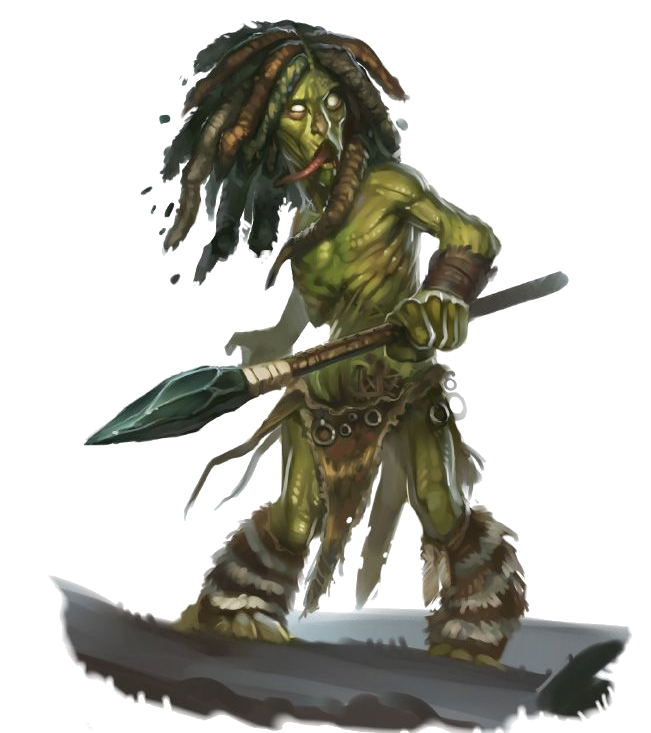
\includegraphics[width=0.48\textwidth]{04kins/img/15naenk_warrior.png}
% \end{figure}

\subsection*{Naenk Names}
    Naenks are born without names, and usually remain nameless most of their youth.
    They reach social adulthood by earning a name, which is done either by becoming a warrior or accomplishing a major deed.

    Many naenks live their whole lives unnamed.
    While most accept this reality and become gatherers, it is not uncommon for the nameless to self-exile out of shame or discontent.

    Knaenese is a very hard language to pronounce, so it's common for people of other kins to call naenks by a nickname or a simpler version of their name.

    \paragraph{Names}
    Gantauda, Gesunt, Gunsedant, Hanhant, Hanseek needa, Hantadage, Huntge, Keena, Kegunseeda, Knaetseeknan, Knandage, Knudu, Kueqan, Nade, Naekuntge, Nega, Nelati, Seetun, Tsaegae, Tsege, Tsehant, Ukena.

\subsection*{Traits}
    Your naenk character has an assortment of abilities, relating to their nature and surroundings.

    \subparagraph{Ability Score Increase} Your Dexterity score increases by 2.

    \subparagraph{Age} A naenk typically lives at most 30 years.
    They are naturally mature right after being born and usually take less than a month to adapt to their society.

    \subparagraph{Alignment} Naenks are organized creatures, used to following the rules of their communities.
    Most tend towards the silver tide, especially those who haven't gained a name yet.

    \subparagraph{Size} The moss kin come in very varied shapes and sizes.
    They stand a tiny bit smaller than their birth corpse, but weight about half.
    Your size and anatomy varies greatly depending on your birth corpse. \label{kin::naenk.size}

    \subparagraph{Speed} Your base walking speed is 6 meters.

    \subparagraph{Dual Nature} You are both humanoid and plant.

    \subparagraph{Naenk claws} Because of your sharp claws, you have a base climbing speed of 6 meters.
    In addition, your claws are natural weapons, which you can use to make unarmed strikes.
    If you hit with them, you deal slashing damage equal to 1d4 + your Strength modifier, instead of the bludgeoning damage normal for an unarmed strike.

    \subparagraph{Eat by Osmosis} While naenks prefer to eat meat by nature, you can mostly live off nutrients from the ground.
    When in fertile land, you only need to eat once per week.
    You can also eat more often if you choose to do so.

    \subparagraph{Languages} You can speak, read, and write knaenese.
    You can also speak, read, and write other language of your choice, but your pronunciation leaves much to be desired.

    % Despite their lack of lips, the moss kin does speak a language, which is named Knaenese.
    % Knaenese is a very simple, accommodating to their impaired speech.
    % While a naenk can learn other languages, their pronunciation usually leaves much to be desired.

    \subparagraph{Subraces} Naenks are most easily separated by their home - Gannag or Na'ane.

    The most common of their kin, Gannagian naenks are the members of the tribes that surround the Tekatsae tree.
    They have a very strong sense of community and an excellent capacity to work as a team.
    Any one naenk will easily give their life without second thought for their people and for their way of life.

    While all naenks are capable fighters, Gannagian naenk take on different jobs to fulfill different tasks.
    The most common of these are the warriors, the hunters, and the gatherers.
    Your subrace traits depend on which of these roles you take.

\subsubsection{Gannagian Warrior}
    \subparagraph{Ability Score Increase} Your Strength score increases by one.

    \subparagraph{Moldy Companion} As part of a long rest, you may contaminate a recently deceased beast with nanust spores.
    To do this, you must succeed on a medicine ability check of DC 8 + the creature's number of hit dice.
    If you succeed, the spores will settle into the beast, and the corpse rises as your nuen at the end of the long rest.

    The nuen has the stats, abilities, and actions of the original beast, but its hit points and hit dice are cut in half.
    It acts on its own volition and on its own initiative turn, but you can use an action to issue an order to it, which it follows to the best of its abilities.
    It also gains the Plant Camouflage trait (page \pageref{trait::plantcamouflage}).

    When travelling with one or more gannagian warriors, only the naenk with the highest Wisdom score can use this trait.

    \subparagraph{Combat Training} The damage die of your claws is increased from a d4 to a d6.
    Additionally, you can choose to add your Dexterity bonus rather than your Strength bonus to your attack and damage rolls.
    % Trained and proficient in combat, you know the first rank of the \textbf{Armed Fighter} feat (page \pageref{feat::armedfighter}).

\subsubsection{Gannagian Hunter}
    \subparagraph{Ability Score Increase} Your Constitution score increases by one.

    \subparagraph{Plant Camouflage} You have advantage on Dexterity (Stealth) checks you make while in any terrain with ample obscuring plant life. \label{trait::plantcamouflage}

    \subparagraph{Hunter's Guts} You are competent in the Survival skill.
    Additionally, your base climbing speed is increased to 9.

\subsubsection{Gannagian Gatherer}
    \subparagraph{Ability Score Increase} Your Intelligence score increases by one.

    \subparagraph{Darkvision} Gatherers spend most of their life recollecting fungus underground, which provides you with an increased awareness in the dark.
    You can see in dim light within 12 meters of you as if it were bright light, and in darkness as if it were dim light.
    You can't discern color in darkness, only shades of gray.

    \subparagraph{Seedspeech} Through sounds and touch, you can communicate simple ideas to living plants, and are able to interpret their responses as simple language.
    Plants do not perceive the world in terms of sight, but most can feel differences in temperature, describe things that have touched them, as well as hear vibrations that happened around them (including speech).

\subsubsection{Na'anian Naenk}
    Among the naenks that grow disillusioned with their tribes, many choose to pack their possessions and leave.
    Among these self-exiled naenks, most usually choose to join the neighboring nation of Na'ane to live with their tsanek brothers.

    These naenks drink a special beverage upon arrival known as nahan cooked by the nations sovereigns.
    % NOTE. Nahan literally means "I-water" in Knaenese.
    Nahan weakens the bond of the naenk with the Tekatsae tree, forcing them to attain a qualar to remain sentient.
    % As a side effect, it also extends the naenk's life, pushing it to about 50 years.

    \subparagraph{Ability Score Increase} You are learned the way of the tsaneks, and your Wisdom score increases by one.

    \subparagraph{Rapport Spores} Your time among the tsaneks has allowed your body to adapt, and fungal growths are found all around your body.
    You can extend rapport spores in a 4.5 meter radius as an action.
    These spores go around corners and affect any creatures with an Intelligence score of 2 or more that aren't undead, constructs, or elementals.
    Creatures affected by the spores realize the effect immediately, but those outside of range cannot notice it.
    Affected creatures can communicate telepathically with one another while they remain within 6 meters of each other.
    The effect lasts for 15 minutes.

    \subparagraph{Noxious Spores} When a creature touches or hits you with a melee attack, you can choose to secrete noxious spores as a reaction.
    The creature takes 1d6 poison damage if it isn't undead, construct, or elemental.
    You can use this skill a number of times equal to your Constitution modifier (minimum of 2).
    After expending all uses, you can't use this trait again until you complete a short rest.

% \begin{figure}[!b]
%     \centering
%     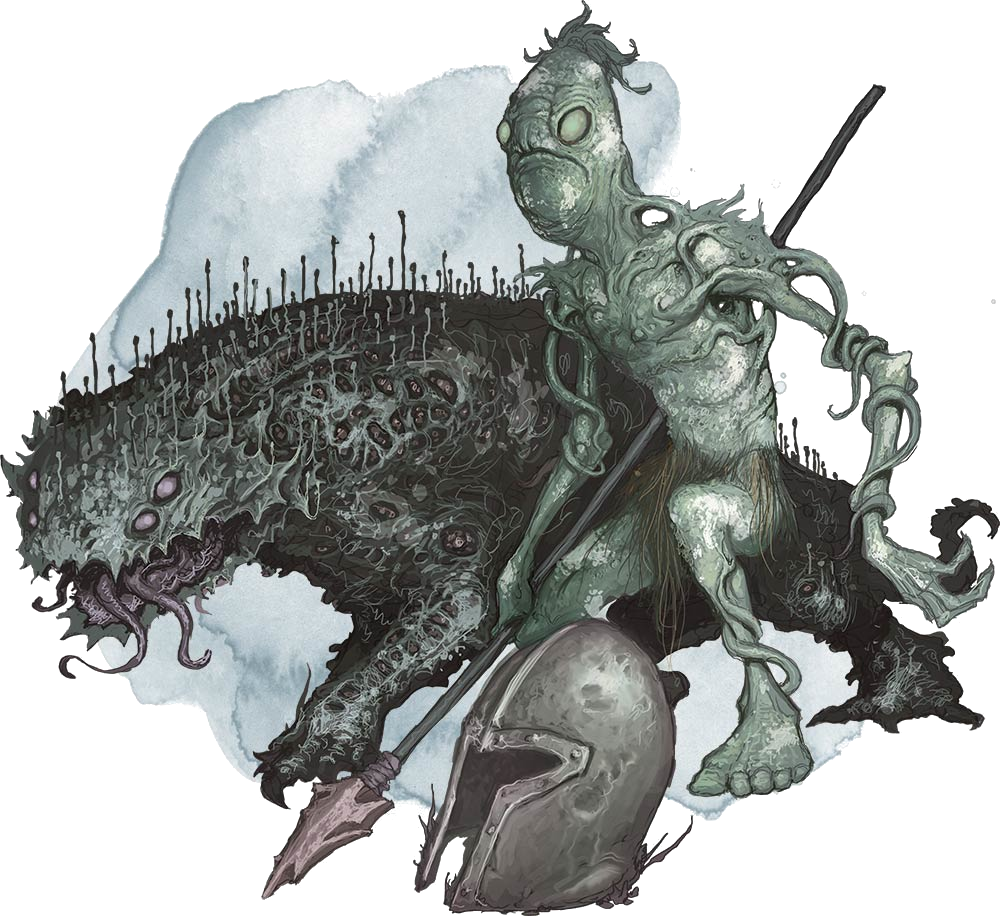
\includegraphics[width=0.48\textwidth]{04kins/img/15naenk_nuen.png}
% \end{figure}

\newpage~\newpage

% !TEX root = ../main.tex
\section{Fungal Kin} \label{kin::tsanek}
\DndDropCapLine{I}{ done seen some things down there.}
\textit{There be cities grander than any of gat's make, holdin' creatures stranger than the harrowing immensity isself.
There be ungodly abominations that weren't never meant to see the light o' day.
And there be... there be mushrooms! An entire city of mushrooms!}

\hspace*{\fill} --- Blim, the Na'anian chronicles.

% TODO: MOVE TO TSANEK SECTION!

% Apart from its chief, every unit has a designated tsanek shaman.
% This tsanek is mainly in charge of communicating with the other tsaneks in faraway places, aiding in the coordination of the tribe as a whole.
% Apart from this and other ceremonial tasks, the shaman acts as a normal member of the unit.

% The highest ranking members of their society are the sovereigns and elder sovereigns, who are tsaneks that reached their final stage of development.
% The former are huge mobile tsaneks that take root in strategic positions in Drejeck to establish their complex communication network.
% The latter are the eldest in the tribe, and merge with Tekatsae itself.
% They directly speak to the tree, communicating its wishes to the sovereigns and shamans via their root network.

Also known as tsaneks in the naenk tongue, the fungal kin is a species of intelligent fungi creature that inhabit swamps, forests, and caverns.
They are commonly seen in the jungle of Drejeck, as members of the tribes near the tekatsae tree.
Like the naenks, tsaneks grow from the tree itself, starting out as small russet-colored fungi in the tree's base and exposed roots, until they're able to grow legs and emerge.
Unlike the naenks, the fungal kin are capable of reproducing by themselves, and it's very common to find independent tsanek communities in the darker reaches of Yuadrem.

Tsaneks generally deplore violence, and only attack when provoked.
If approached peacefully, they gladly provide shelter or passage through their colonies.

\subsection*{Tribal Life}
    Most tsaneks belong to the tribes of Drejeck, filling the roles of shamans and diplomats that the naenks are less likely to fulfill due to their violent nature.
    They are considered above their mossy companions in their social circles, and are generally treated with respect among them.

    When a tsanek reaches 100 years, it is put through the rite of growth.
    The tsanek must ceremoniosly consume a mixture of the sap of tekatsae, wyvernroot, and water of the boiling river. % Wyvernroot is a strong poisonous plant native to Drejeck.
    Next, it must enter a chamber of awareness, which are small caverns below tekatsae.
    The tsanek is only left out after a month in isolation.
    Most of the tsaneks that go through this ritual die, and are consumed by tekatsae, bringing them back to the tree.
    The ones that don't become the highest ranking members of their tribal societies: Sovereigns.
    Tsanek sovereigns are large, malformed creatures that reign over the tribes.
    They are the only creatures capable of directly speaking with tekatsae, and thus are the only that can communicate its wishes to the tribes.

\subsection*{Circles and Melds}
    Many tsaneks, feeling unprepared, leave the tribes before this ritual.
    Usually many more of their species follow them to start independent communities as exiles.
    Over a timeframe of 300 to 400 years, the eldest from these colonies naturally grow to become sovereigns themselves, presiding over many social groups called circles.
    A circle consists of twenty or more fungal kin that work, live, and meld together.

    Melding is prohibited in the Drejeck tribal communities, but is a regular practice in these circles.
    A meld is a form of communal meditation that allows tsaneks to transcend their sometimes dull existence.
    Their rapport spores bind the participants into a group consciousness, inducing a shared dream that provides entertainment and social interaction.
    Tsaneks use melding in the pursuit of higher consciousness, collective union, and spiritual apotheosis.
    They can also use their rapport spores to communicate telepathically with other sentient creatures.

\subsection*{Tsanek Reproduction}
    Like other fungi, tsanek reproduce by mundane sporing.
    They are the only race that can retain their sentience without qualar, but if their spores grow without the influence of tekatsae or a particularly old sovereign, the sprouting quickly becomes feral, unable to retain sentience.
    Due to this, tsaneks carefully control their spores' release.

    Tsaneks are known to feel very little connection to their offspring.
    Among the tribal tsaneks, the children of their species are taken care of by a few tsanek designated as the spore-caretakers.
    Among the exiles, child rearing becomes a responsbility shared by the entire circle.
    It is rare if young tsaneks can even identify their parents.

\subsection*{Call to Adventure}
    While many tsanek are needed in the tribes near tekatsae for managerial tasks, it is not unusual for some to travel the globe to learn.
    Most focus their study on the qualar and cter'rheth, bringing this knowledge back to their tribes.

    Cavern tsaneks regularly travel the many caves below Yuadrem, and some even settle outside of their colonies, most usually in dark gat cities.
    Some have founded libraries, laboratories, and monasteries, usually along oths, and dedicate their lives to research and education.

\subsection*{Tsanek Names}
    Due to the fact that tsaneks have no verbal language, their names are most appropriately translated as physical descriptions of a particular individual.

    \paragraph{Names}
    Bolete, Brownback, Buttonhead, Greenfoot, Morel, Mossy, Portabelt, Puffball, Redstem, Soft-Step, Stinkhorn, Toad.

\begin{figure}[!t]
    \centering
    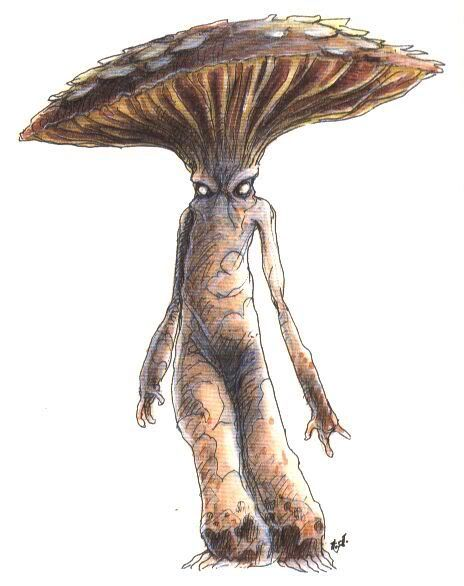
\includegraphics[width=0.48\textwidth]{04kins/img/16tsanek_individual.jpg}
\end{figure}

\subsection*{Traits}
    Your tsanek character has a diverse set of skills based on its nature and role on society.

    \subparagraph{Ability Score Increase} Your Wisdom score increases by 1, and your Constitution score increases by 1.

    \subparagraph{Size} A tsanek grows to a wide variety of heights and builds, with the most common being stocky and measuring about 1.9 meters in height, weighing around 65 kg.
    Your size is medium.

    \subparagraph{Speed} Your base walking speed is 9 meters.

    \subparagraph{Age} Individual tsanek are not known to die of old age, and the most elder can live to become a sovereign of one or more circles, living indefinitely longer.
    Sproutings take a long time to fully mature, but it's a continuous process and even the oldest tsaneks seem to continue growing, albeit slowly.

    \subparagraph{Alignment} Most often, a tsanek believes strongly in society and law.
    It is extremely uncommon for a tsanek to directly attack any creature that does not mean it, or its circle, harm.
    Most fungal kin groups and circles dedicate their lives to knowledge, and have a tendency towards the blue tide.

    \subparagraph{Nonverbal Magic} Though you have no conventional language, you can ignore the verbal component of spells.

    \subparagraph{Rapport Spores} All creatures within 4.5 meters of you with an Intelligence score of 6 or higher that aren't undead, constructs, or elementals can communicate telepathically with you and with each other if you speak at least one language in common.
    You can suppress this ability at will.
    Creatures affected by the spores realize the effect immediately, but those outside of range cannot notice them.
    Affected creatures can communicate telepathically with one another while they remain within 9 meters of each other.

    \subparagraph{Pacifying Spores} As two actions, you can eject spores at one creature you can see within 1.5 meters of you.
    The target must succeed on a Constitution saving throw or be stunned for 1 minute.
    The spell save DC for this effect is 8 + your Constitution modifier.
    Undead, constructs, and elementals automatically succeed on this save.
    The target can repeat the saving throw at the end of each of its turns, ending the effect on itself on a success.
    After using this trait, you cannot do so again until you finish a short rest.

    \subparagraph{Hallucination Spores} As an action, you can produce spores that affect all creatures within 9 meters of you that aren't undead, constructs, or elementals.
    These creatures are all affected as per the cantrip minor illusion while you concentrate on the effect, which you can do for up to 1 minute.
    The spell save DC is 8 + your Constitution modifier.

    \subparagraph{Languages} You can understand, read and write knaenese and one other language of your choice, but you cannot speak.

    \subparagraph{Feats} From your kin, the feats available to you are
    \textbf{} (page \pageref{feat::}),
    \textbf{} (page \pageref{feat::}),
    \textbf{} (page \pageref{feat::}),
    \textbf{} (page \pageref{feat::}),
    \textbf{} (page \pageref{feat::}),
    \textbf{} (page \pageref{feat::}), and
    \textbf{} (page \pageref{feat::}).

\begin{table*}[b]%
    \begin{DndTable}[width=\linewidth]{X}
        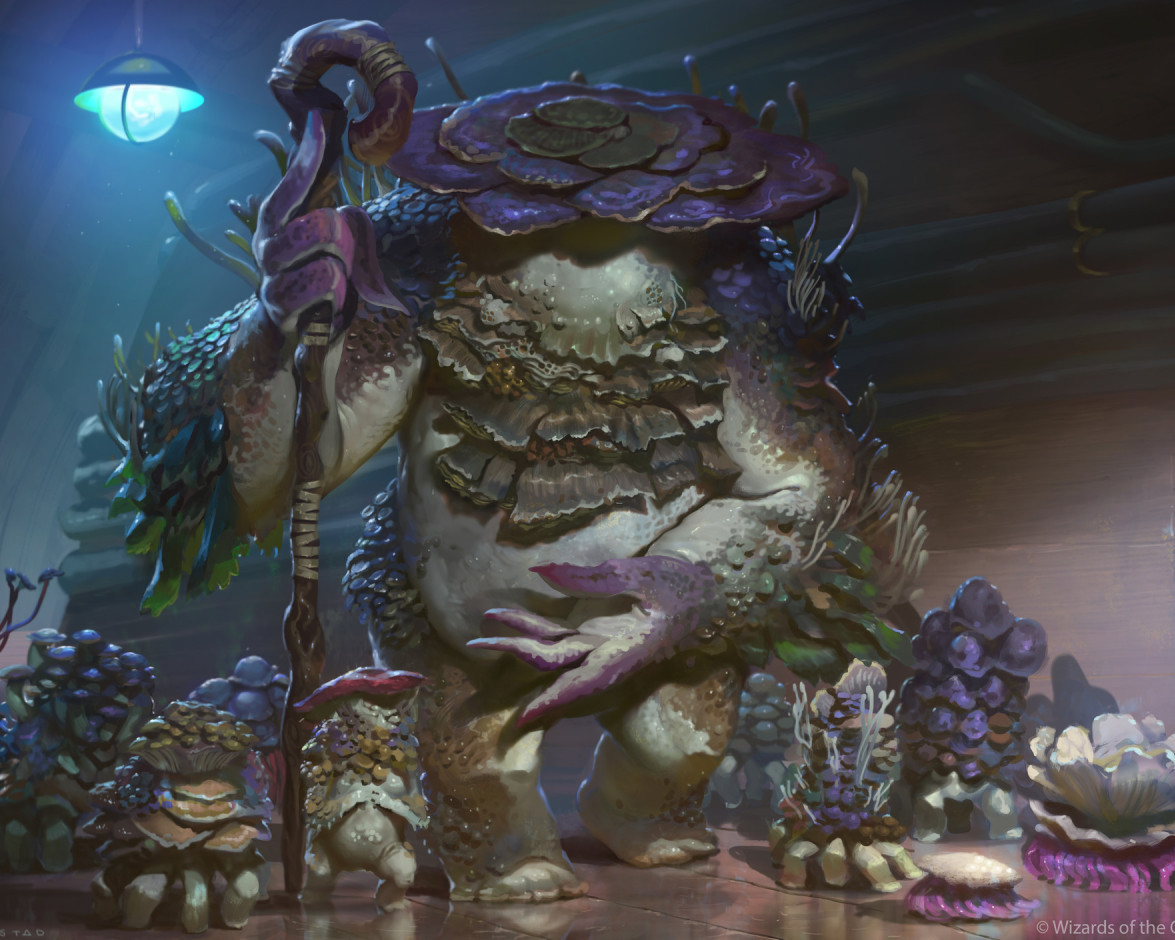
\includegraphics[width=0.98\textwidth]{04kins/img/16tsanek_sovereign.jpg}
    \end{DndTable}
\end{table*}

\subsubsection{Gannagian Tsanek}
    Fungal kin that are members of the tribes in Drejeck which surround tekatsae.
    Like their mold kin brothers, they have a very strong sense of community and devotion to their groups, the sovereigns and the tekatsae tree.
    They are the spiritual leaders of the different groups, and focus on coordinating the tribes and communicating with the sovereigns.

    \subparagraph{Ability Score Increase} You focused much of life in study, and your Wisdom score increases by 1.

    \subparagraph{Drug-enhanced Spores} Your Rapport Spores' range is increased to 9 meters.
    The spell save DC of all your spores is increased by 2.

    \subparagraph{Euphoria Spores} Accustomed to fighting with the naenk warriors, you can release a specialized cloud of spores in a 6-meter-radius sphere centered on yourself.
    Other creatures in the area must make a Constitution saving throw of a DC equal to 8 + your Constitution modifier or become poisoned for 1 minute.
    A creature can repeat this saving throw at the end of each of its turns, ending the effect early on itself on a success.
    When the effect ends, the creature gains one level of exhaustion.
    You can produce these spores a number of times equal to your Constitution modifier (minimum of 1) per long rest.

    \subparagraph{Feats} From your subrace, the feats available to you are
    \textbf{} (page \pageref{feat::}),
    \textbf{} (page \pageref{feat::}), and
    \textbf{} (page \pageref{feat::}).

\subsubsection{Na'anian Tsanek}
    Sometimes, a tsanek will decide to abandon the tribe and break its link with the tekatsae tree.
    These tsanek, unable to forgo their community lifestyles, tend to join or form fungus kin communities in the caverns of the world, sometimes spawning huge underground fungus cities.

    \subparagraph{Ability Score Increase} Your meandering in hostile environments has granted you increased resilience, and your Constitution score is increased by 1.

    \subparagraph{Sun Sickness} You become poisoned if you spend more than 1 minute in direct, unobstructed sunlight.
    This conditions ends when you spend 1 minute in dim or dark conditions.

    \subparagraph{Superior Darkvision} Accustomed to the darkness of the deepest of caverns, you have superior darkvision in dark and dim conditions.
    You can see in dim light within 36 meters of you as if it were bright light, and in darkness as if it were dim light.

    \subparagraph{Meld} When you take a short rest in the presence of one or more other tsaneks, you can meld with them.
    After melding, you and all melding tsaneks regain all expended Hit Dice and gain the following benefits:
    \begin{itemize}
        \item You have advantage on a saving throw you make in the next 24 hours.
        \item You can end one disease or condition affecting you, be it blinded, deafened, paralyzed, or poisoned.
    \end{itemize}

    \subparagraph{Communal Intellect} Your time spent melding with the others of your kin has granted you a deeper understanding of the world and yourself.
    You are competent in the Insight and Religion skills, and you have advantage on Wisdom (survival) checks made to find your way in caverns.

    \subparagraph{Feats} From your subrace, the feats available to you are
    \textbf{} (page \pageref{feat::}),
    \textbf{} (page \pageref{feat::}), and
    \textbf{} (page \pageref{feat::}).

\newpage

% !TEX root = ../main.tex
\section{Shelled Kin} \label{sec::shelledkin}

\textit{I caught a big fish.}

\textit{Now I search for a good friend}

\textit{To share my lunch with.}

\hspace*{\fill} --- Tortle haiku.

The shelled kin are a species native to the Underworld.
Also known as tortles, they have gracefully adapted to their lives in Yuadrem, able to start a new life in the land ravaged by the schism, and it is very common to see the rustic tortle villages in the coasts of the beryl sea and many of the eastern shores of the continent.
% The shelled kin or tortles are a species native to the Underworld which, unlike umans, don't seem to be hunted by the strange creatures from this place, and remain unaffected by the forbidden lands.

What many tortles consider a simple life, others might call a life of adventure.
Tortles are born near sandy coastlines, but as soon as they're able to walk on two legs, they turn into nomad survivalists eager to explore the wilderness, experience its many wonders, put their skills to the test, and make new acquaintances.

\begin{figure}[!b]
    \centering
    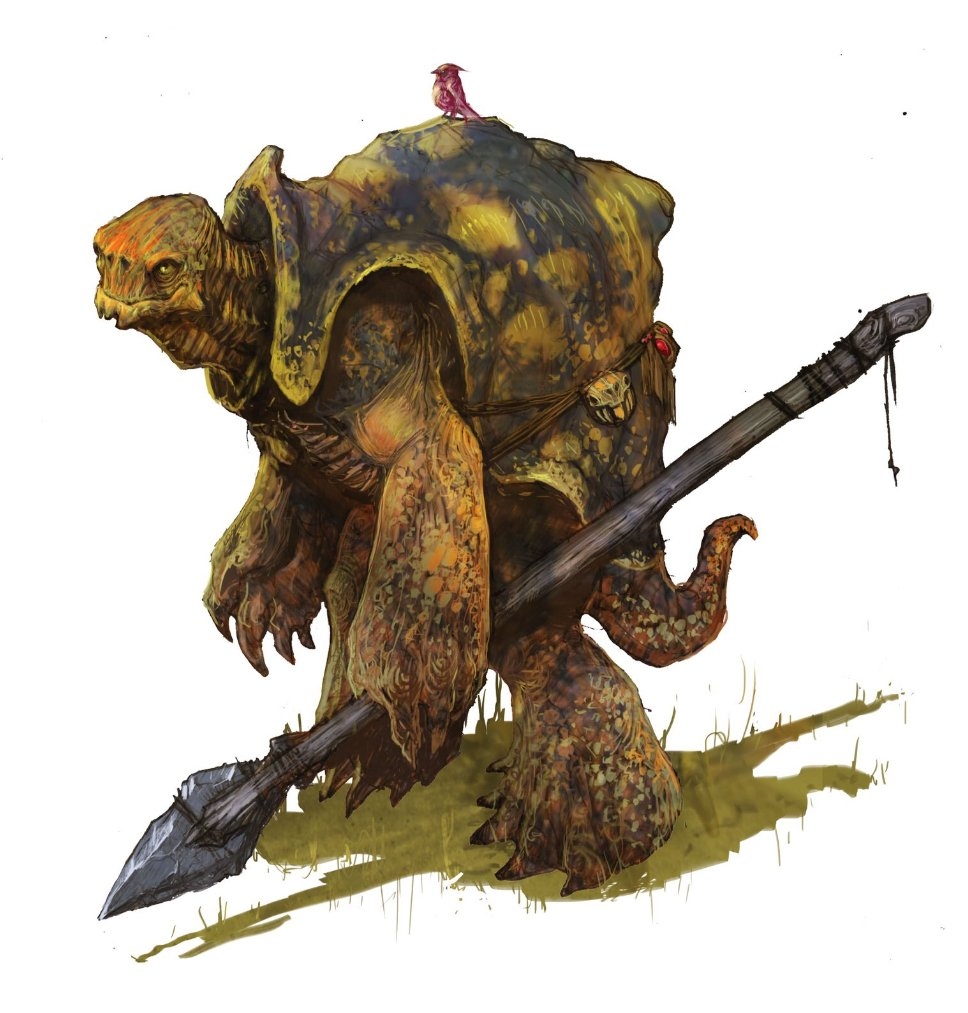
\includegraphics[width=0.48\textwidth]{04kins/img/17tortle_official.jpg}
\end{figure}

\subsection*{Life of a Tortle}
A tortle hatches from a thick-shelled egg and spends the first few weeks of its life crawling on all fours.
Its parents usually leave soon after its birth, but spend what little time they have telling stories to their offspring.
Within a year, the young tortle is abandoned and becomes an orphan, though not before it learns to speak and to survive on its own.

A young tortle and its siblings inherit whatever tools, weapons, and gifts their parents leave for them.
Each young tortle is expected to fend for itself.
It leaves the place of its birth and finds its own corner of the wilderness in which to hunt, catch fish, and get by.
With each passing year, a tortle hones its survival skills.
It forms friendships with its neighbors while also respecting their privacy.
At some point, a tortle feels an almost overwhelming urge to venture far away from home and see more of the world.
It gathers up its possessions and heads into the wilderness, returning months or years later with stories of its exploits and new skills.

Tortles are gendered creatures, and it is usual for them to seek out a mate and procreate when they return home from these travels.
Tortles lay their eggs (numbering as few as one or as many as a dozen) in a fortified compound enclosed by stone walls that are easily defensible.
If no such compound exists, they build one.
The parents spend the hatching time of their eggs guarding the compound and defending their offspring, and after they hatch they spend a year sharing their knowledge with the young ones.
The parents leave their children at this time, overburdened by their nomadic nature and confident that the older tortles of the village will care for them.
When the children are old enough to leave the compound, they pick up whatever weapons and tools their parents left behind and set out on their own.

\subsection*{Beliefs}
Tortles don't have a religion of their own, but they often worship the gods of other races.
It's not unusual for a tortle to hear stories or legends related to a god and choose to worship that deity.
Curious in nature, most tortles like to see how other creatures live and discover new customs and new ways of doing things.
Some tortles are also drawn to the many schools of thought, trying to learn from all of them instead of focusing on a single one.

Tortles believe that night and day watch over them and other creatures.
The moons are the eyes of night that watch over them in darkness, and the sun is the equally vigilant eye of day.
Tortles feel most at peace when these ``eyes'' are looking down on them.
They become more nervous and uneasy when no orb is visible in the sky.
Tortles tend to be most uncomfortable underground, where neither the sun nor the moons are visible to them.

Blessed are the days when many moons are visible in the sky at the same time.
Tortles often choose such days to leave their homes and begin a wilderness expedition, or perform some other task they know to be dangerous.

\subsection*{Inherent Mutualism}
Tortles have a special relationship to the anchelons.
Anchelons are colossal horned turtles that reside in Yuadrem's oceans, breeding fear among sailors and fishers alike.
They are generally fierce in nature but, while not sentient, they are oddly friendly toward tortles.
Anchelons lay their eggs in the beryl sea, and tortles allow thme to lay their eggs in their compounds.
It is not uncommon for baby anchelons to grow alongside tortles.
Anchelons in exchange protect the tortles' villages, and may even help tortles they encounter in the wilds.

\begin{table*}[b]%
    \begin{DndTable}[width=\linewidth]{X}
        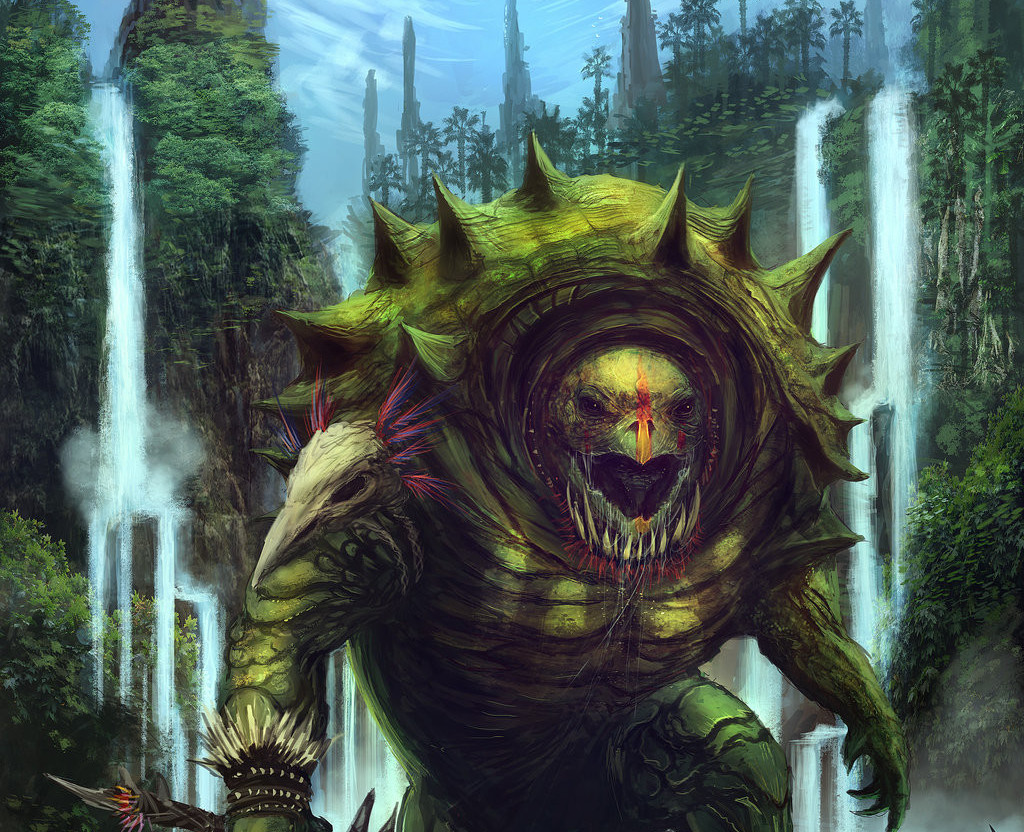
\includegraphics[width=0.98\textwidth]{04kins/img/17tortle_spiked.jpg}
    \end{DndTable}
\end{table*}

\subsection*{Adventurers at Heart}
Tortles have a saying: ``We wear our homes on our backs''.
The shells they carry around provide all the shelter they require.
Consequently, tortles don't feel the need to root themselves in one place for too long.
A tortle settlement is primarily used as a kind of moot, where tortles can socialize with one another, share useful information, and trade with strangers in the safety of greater numbers.
Tortles don't regard these settlements as places worth defending with their lives, and they will abandon a settlement when it no longer serves their needs.

Tortles embrace a simple view of the world.
It is a place of wonder, and tortles see beauty in the ordinary.
They live for the chance to hear a soft wind blowing through palm trees, to watch a frog croaking on a lily pad, or to stand in a crowded marketplace.

Tortles like to learn new skills.
They craft their own tools and weapons, and they are good at building structures and fortifications.
They marvel at the works of other kins, and can lose themselves for years in a city, studying its architectural wonders and learning skills they can put to use when building forts to contain their offspring.

Although they spend a considerable portion of their lives in isolation, tortles are social creatures that like to form meaningful friendships.
Being native to another world, they have no inbred animus toward any kin.
In fact, a tortle will often seek out friendships with non-tortles to learn new customs and new points of view.

% \begin{figure}[!htbp]
%     \centering
%     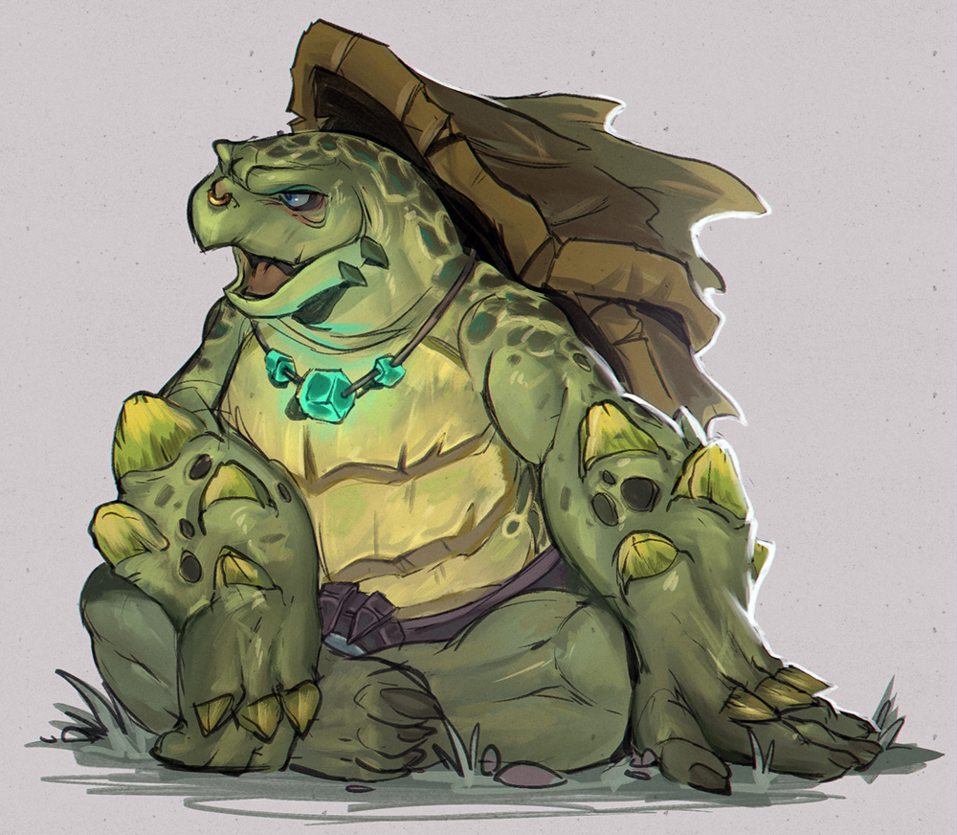
\includegraphics[width=0.48\textwidth]{04kins/img/tortle_chill.png}
% \end{figure}

\subsection*{Tortle Names}
Tortles prefer simple, non-gender-specific names that are usually no more than two syllables long.
If a tortle doesn't like its name for whatever reason, it can change it, and it might do this a dozen times in its life.

A tortle doesn't feel constrained by its name, which is designated only to refer to the tortle in contrast of its peers.
Tortles don't have surnames or family names.

\paragraph{Names}
Baka, Damu, Gar, Gura, Ini, Jappa, Kinlek, Krull, Lim, Lop, Nortle, Nulka, Olo, Ploqwat, Quee, Queg, Quott, Sunny, Tibor, Ubo, Uhok, Wabu, Xelbuk, Xopa, Yog

\subsection*{Traits}
Your tortle character gains traits that enable it to cope with the perils of a savage world.

\subparagraph{Ability Score Increase} Your Strength score increases by 2, and your Wisdom score increases by 1.

\subparagraph{Age} Young tortles crawl for a few weeks after birth before learning to walk on two legs.
They reach adulthood by the age of 15 and live an average of 500 years.

\subparagraph{Alignment} Tortles tend to lead orderly, ritualistic lives.
They develop customs and routines, becoming more set in their ways as they age.
Most follow a set of tenets that the kin brought with them from the Underworld, leading to lawfulness.
While most are good, a few can be selfish and greedy, but it's unusual for a tortle to shuck off order in favor of chaos.
Tortles tend towards the gold tide, always empathic and helping others.

\subparagraph{Size} Tortle adults stand 1.5 to 1.8 meters tall and average 230 kg.
Their shells account for roughly one-third of their weight.
Your size is Medium.

\subparagraph{Hold Breath} Tortles aren't natural swimmers, but they can remain underwater for some time before needing to come up for air.
You can hold your breath for up to 1 hour at a time.

\subparagraph{Natural Armor} Due to your shell and the shape of your body, you are ill-suited to wearing armor.
Your shell provides ample protection, however; it gives you a base AC of 17 (your Dexterity modifier doesn't affect this number).
You gain no benefit from wearing armor, but if you are using a shield, you can apply the shield's bonus as normal.

\subparagraph{Shell Defense} You can withdraw into your shell as an action.
Until you emerge, you gain a +4 bonus to AC, and you have advantage on Strength and Constitution saving throws.
While in your shell, you are prone, your speed is 0 and can't increase, you have disadvantage on Dexterity saving throws, you can't take reactions, and the only action you can take is to use an action to emerge from your shell.

% \subparagraph{Survival Instinct} Tortles have finely honed survival instincts.
% You gain competency in the Survival skill.

\subparagraph{Learned Tradition} You gain competency with either two weapons, two sets of artisan's tools, or one of each of your choice.
This ability comes from the time spent with your parents, and you feel a special connection with these types of items.

\subparagraph{Languages} You can speak the krehlo tongue and one additional language of your choice, but cannot write or read either.
The krehlo tongue doesn't have a written form, and the tortle tenets are passed on in oral tradition.



\newpage

% !TEX root = ../main.tex
\section{Poison Kin} \label{kin::poisonkin}
\DndDropCapLine{T}{hey're a poison spilled down onto}
\textit{ our world, I tell ya'!
Grungs're bad.
They real bad!
They tell ya' their skin be the worst part o'em, but they don't know!
The spears mon.
It's the spears!}

\hspace*{\fill} --- Kleeck recounts her brief visit to Mabela.

Also known as grungs, the poison kin are aggressive creatures that look similar to dart frogs.
The species quickly settled into the chirping wilds and the areas surrounding the rainforest after their arrival during the schism.
They are fiercely territorial and see themselves as superior to most other creatures.

\subsection*{Class Structure}
    Grung society is a caste system.
    Each caste lays eggs in a separate hatching pool, and juvenile grungs join their caste upon emergence from their hatchery.
    All grungs are a dull greenish gray when they are born, but each individual takes on the color of its caste as it grows to adulthood.
    From lowest to highest caste, grungs are green, blue, purple, red, orange, and gold.

    Green grungs are the tribe's warriors, hunters, and laborers, and blue grungs work as artisans and in other domestic roles.
    Supervising and guiding both groups are the purple grungs, which serve as administrators and commanders.
    Red grungs are the tribe's scholars and sorcerers.
    They are superior to purple, blue, and green grungs and given proper respect even by the grungs of higher status.
    Higher castes include orange grungs, which are elite warriors that have authority over all lesser grungs, and gold grungs, which hold the highest leadership positions.
    A tribe's sovereign is always a gold grung.

    A grung normally remains in its caste for life.
    On rare occasions, an individual that distinguishes itself with great deeds can earn an invitation to join a higher caste.
    A mixture of godsblood, seawater and poison is blessed by a red grung, and by drinking it the elevated grung changes color and is inducted into its new caste in the same way that a juvenile of the caste would be.
    From then on, the grung and its progeny are members of the higher caste.

\subsection*{Poisonous Skin}
    All grungs secrete a substance that is harmless to them but poisonous to other creatures.
    A grung can also use this secretion as venom to coat its weapons.
    Grungs are always on the lookout for creatures they can capture and enslave, and use slaves for all manner of menial tasks and hard labor.
    Slaves are fed mildly poisoned food to keep them lethargic and compliant.
    A creature afflicted in this way over a long period of time becomes a shell of its former self, and it seldom can be restored to normalcy.
    Being amphibious, grungs require water to live; any grung that fails to immerse itself in water for at least 1 hour during a day becomes quite exhausted.

\subsection*{Whistle Stick}
    All grungs are trained to use a musical instrument called the whistle-stick.
    This is a hollow wooden tube with holes cut throughout, much like a flute.
    Grungs play music with it for entertainment, but can also swing it about by a sturdy cord to create a sound recognizable by others of their kin, so they know each other's approximate location.
    Additionally, any creature that can speak the krehlo language can use a whistle stick in this manner to communicate over distance.

\subsection*{Outcast or Voyager}
    Since social advancement among grungs can only be achieved by a great deed, it is not unusual for a grung or a small group of them to travel around the coasts and rivers of Yuadrem.
    They attempt to obtain renown by murdering an enemy of their civilization, or by bringing a rare artifact or important strategic information.

    While a rare occurrence, sometimes an individual grung or even entire family-lines can grow disillusioned by the hardships of class advancements.
    Some of them decide to escape from their cities, leading lives of their own as independent colonies or as members of the rare cities or towns willing to accept them.
    Individuals from these groups are known to follow a life of adventure to help their communities or simply to satiate an internal need for excitement in the grung's heart.

\subsection*{Grung Names}
    Grungs usually have simple, non-gender-specific names with a strong consonant joined by a syllable with a glottal stop, but members of higher castes prefer longer, more elaborate names to reflect their status.
    Their names don't actually come from the krelho language, but are made based on what's easier to pronounce for the grung.
    Grungs also wear their city of origin as surname.

    \paragraph{Names}
    B'ang, B'leep, B'lip, B'loop, Bl'eg, Bl'myeek, Bl'ngiip, Ch'eg, Ch'rol, D'aht, D'khan, F'huu, Fl'aak, Fl'uup, G'lahp, Gh'rol, K'eet, K'riig, K'ung, R'ang, R'loo.

    \paragraph{Surnames}
    Bakagar, Bomqueeg, Gor, Int, Joppank, Kangaru, Limlim, Mabela, Obu, Om, Ploqlek, Queequio, Quott'nem, Uhok'moa, Wewat, Xilkoko, Zipqueg.

\begin{figure}[!t]
    \centering
    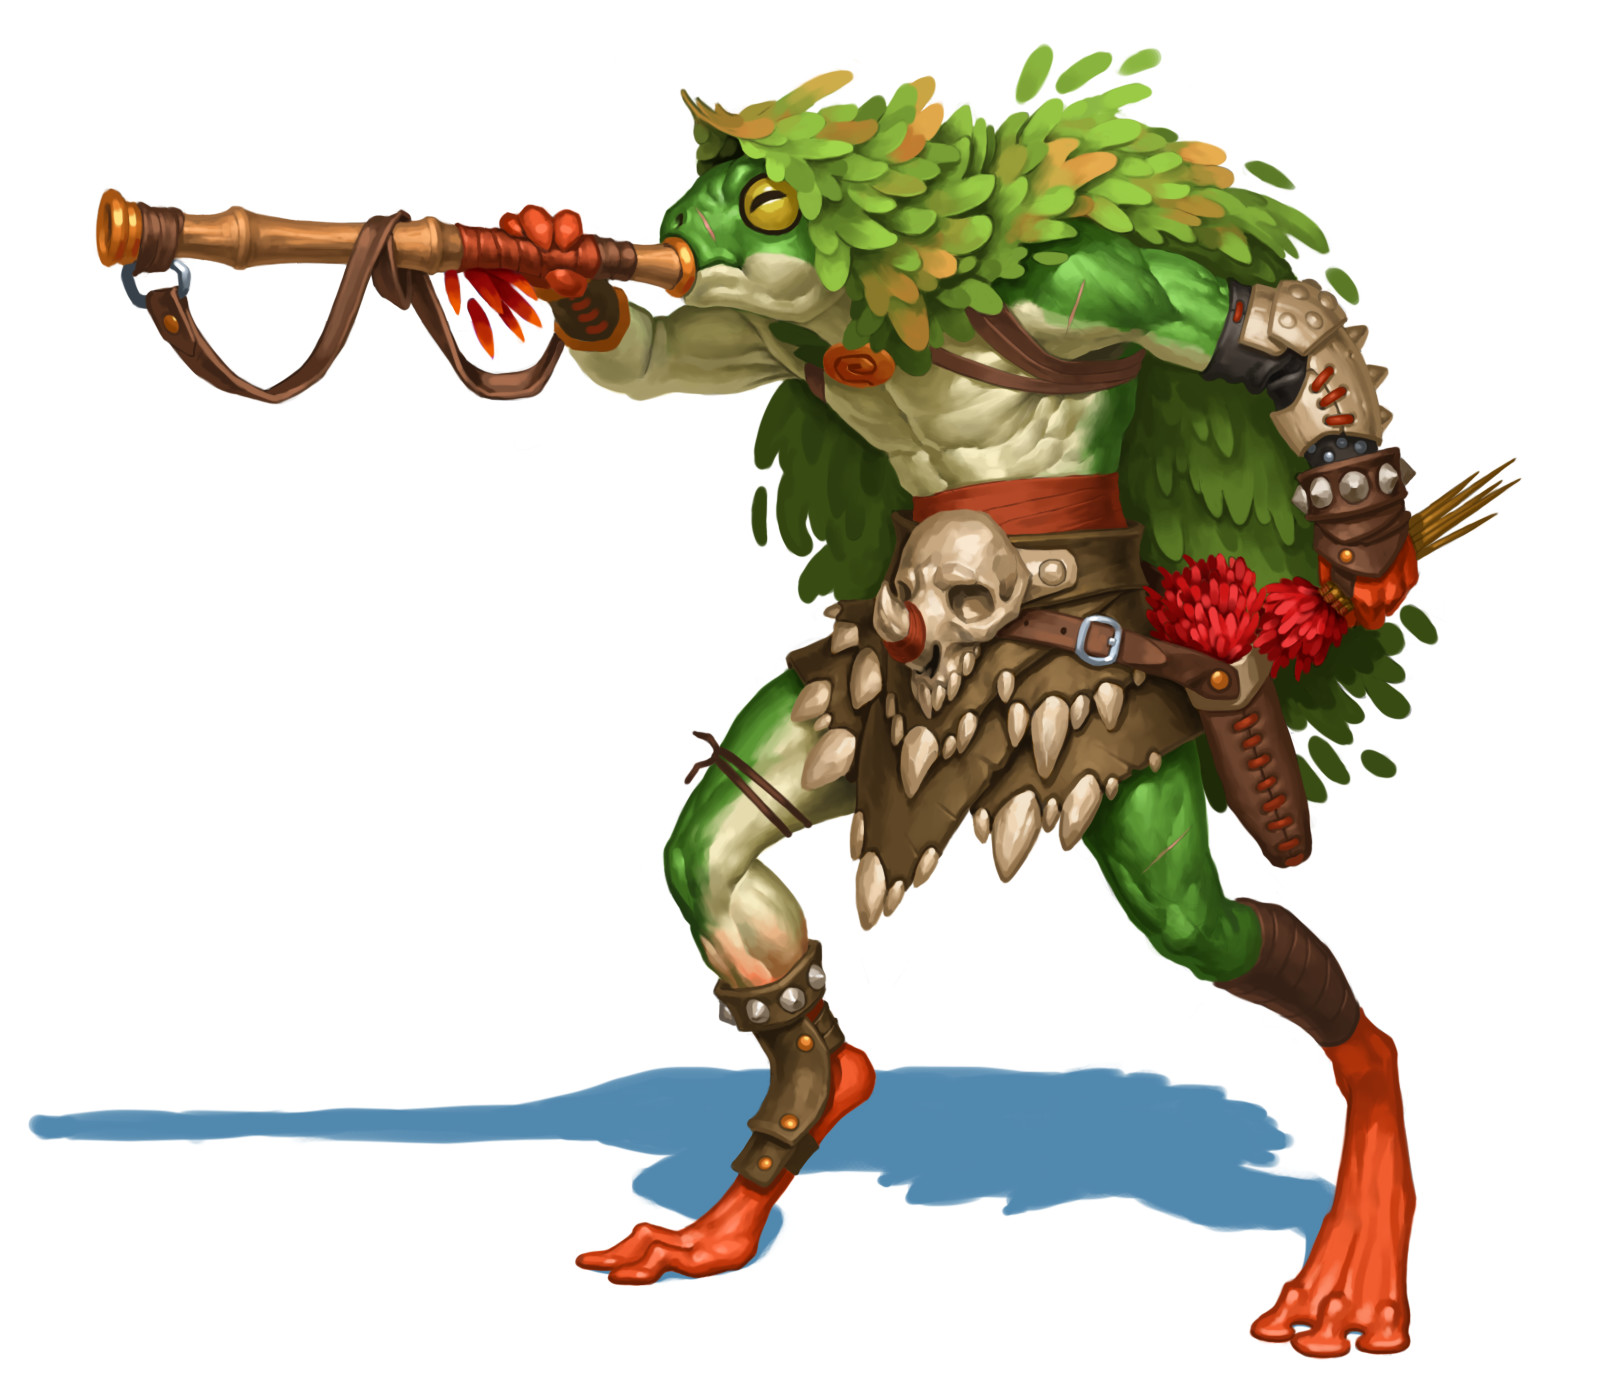
\includegraphics[width=0.48\textwidth]{04kins/img/18grung_blowgun.jpg}
\end{figure}

\subsection*{Traits}
    Your grung character has an assortment of inborn abilities, part and parcel of grung nature:

    \subparagraph{Ability Score Increase} Your Dexterity score increases by 2, and your Constitution score increases by 1.

    \subparagraph{Age} Grung reach adulthood in a single year, and can live for up to 80 years.

    \subparagraph{Alignment} % Most grungs are lawful, having been raised in a strict caste system.
    % Grung society is in constant search of power, and most individual grung look forward to very rare social advancement.
    Grungs are in constant search of power, and move along the silver tide.

    \subparagraph{Size} Grungs stand between 75 and 105 cm tall and average about 20 kg.
    Your size is small.

    \subparagraph{Speed} Your base walking speed is 5 meters, and you have a swimming speed of 5 meters.

    \subparagraph{Amphibious} You can breathe both air and water.

    \subparagraph{Poison Resistance} You are resistant to poison damage.

    \subparagraph{Poisonous Skin} Any creature that grapples you or otherwise comes into direct contact with your skin must succeed on a Constitution saving throw of DC 8 + your Constitution modifier, taking 2d4 poison damage and becoming poisoned for 1 minute on a fail.
    A poisoned creature no longer in direct contact with you can repeat the saving throw at the end of each of its turns, ending the effect on a success.

    You can also apply this poison to a slashing weapon, a piercing weapon, or three pieces of ammunition using two actions.
    % The target must succeed on the same saving throw or take 2d4 poison damage.
    A grung succeeds on these saving throws automatically.

    You can choose to add an additional effect that varies depending on your skin color.
    This effect lasts until the end of your next turn.

        \paragraph{Green Toxins} The poisoned creature can't move except to climb or make standing jumps.
        If the creature is flying, it can't take any actions or reactions unless it lands.

        \paragraph{Blue Toxins} The poisoned creature must shout loudly or otherwise make a loud noise at the start and end of its turns.

        \paragraph{Purple Toxins} The poisoned creature feels a desperate need to soak itself in liquid or mud.
        It can't take actions or move except to do so or to reach a body of liquid or mud, unless no such body can be found in a 18 meter radius.

        \paragraph{Red Toxins} The poisoned creature feels extreme hunger and must use its action to eat something or to move towards a source of food, unless no source of food can be found in a 18 meter radius.

        \paragraph{Orange Toxins} The poisoned creature becomes frightened of its allies.

    \subparagraph{Standing Leap} Your long jump is up to 5 meters and your high jump is up to 3 meters, with or without a running start.

    % \subparagraph{Grung Weapon Training} Due to combat training, you are proficient with spears, blowguns, and nets.

    \subparagraph{Inflatable Cheek Pouches} Due to your frog-like anatomy, you are able to shoot darts at incredible speed.
    You are competent with blowguns, and with it you can shoot darts to a range of 10/20 meters.
    Additionally, you can apply your poison to the darts as part of your attack with them.

    % \subparagraph{Water Dependency} If you fail to immerse yourself in water for at least 1 hour during a day, you suffer one level of exhaustion at the end of that day.
    % You can only recover from this exhaustion by immersing yourself in water for at least 1 hour.

    \subparagraph{Languages} You can speak the krehlo tongue and one additional language of your choice, but cannot write or read either.

\begin{figure}[!b]
    \centering
    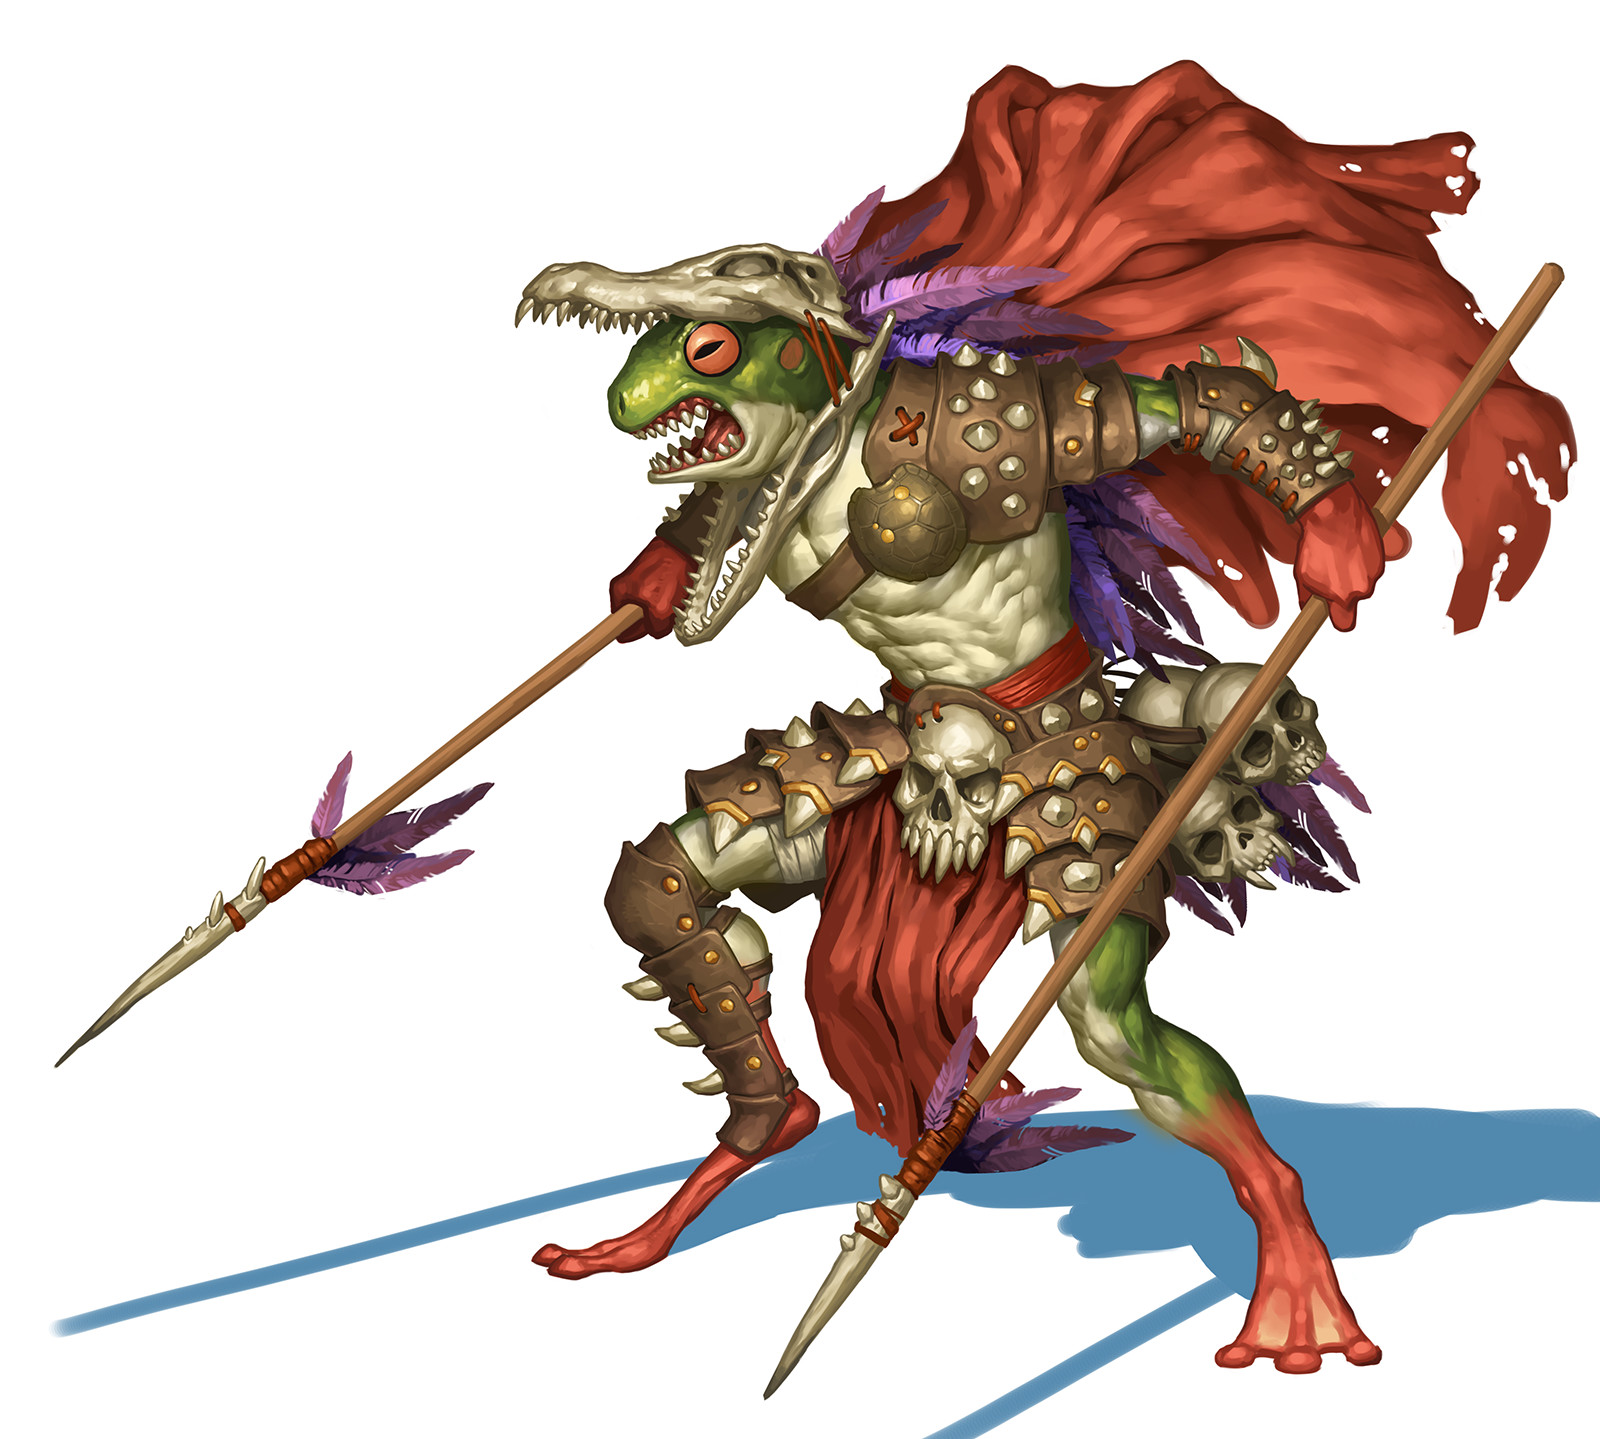
\includegraphics[width=0.48\textwidth]{04kins/img/18grung_warrior.jpg}
\end{figure}

\newpage

\subsection*{Grung Feats}
    \begin{DndTable}[width=\linewidth, header=Grung Feats]{ll}
        Grung & \textbf{Arboreal Alertness} (page \pageref{feat::arborealalertness}) \\
        Grung & \textbf{Gold Toxin} (page \pageref{feat::goldtoxin})                 \\
        Grung & \textbf{Hardy} (page \pageref{feat::hardy})                          \\
        Grung & \textbf{Mesmerizing Chirr} (page \pageref{feat::mesmerizingchirr})   \\
        Grung & \textbf{Mirthful Leaps} (page \pageref{feat::mirthfulleaps})         \\
        Grung & \textbf{Moist Skin} (page \pageref{feat::moistskin})                 \\
        Grung & \textbf{Poison Immunity} (page \pageref{feat::poisonimmunity})       \\
        Grung & \textbf{Slippery Skin} (page \pageref{feat::slipperyskin})           \\
        Grung & \textbf{Toxic Skin} (page \pageref{feat::toxicskin})                 \\
        Grung & \textbf{Waterbound} (page \pageref{feat::waterbound})
    \end{DndTable}

    \subsubsection{Arboreal Alertness} \label{feat::arborealalertness}
        As long as you are not already an Expert, you increase your level of competence in the Perception skill.
        Additionally, you gain a +5 bonus to your passive Wisdom (Perception) and passive Wisdom (Insight) when in forested areas.
        \paragraph{Requirements} Grung kin or Boggart subrace.
    \subsubsection{Gold Toxin} \label{feat::goldtoxin}
        You learn how to excrete the rarest of grung poisons, the gold toxin.
        Once per long rest, you can choose to use a gold toxin when you use your poisonous skin trait.
        The DC from your \textbf{Poisonous Skin} trait increases by 2, and on a failure the creature is charmed for a minute.
        The creature can repeat this saving throw at the end of its turns.
        Additionally, it permanently learns how to speak basic krehlo.
        \paragraph{Requirements} Grung kin.
    \subsubsection{Mesmerizing Chirr (2 FP)} \label{feat::mesmerizingchirr}
        You make a chirring noise to which grungs are immune.
        Each humanoid or beast that is within 3 meters of you and able to hear you must succeed on a DC 10 + your Constitution modifier Wisdom saving throw or be stunned until the end of your next turn.
        You can use this ability a number of times equal to your Constitution modifier (minimum of 1), and recover all expended uses at the end of a short rest.
        \paragraph{Requirements} Grung kin.
    \subsubsection{Moist Skin} \label{feat::moistskin}
        As an action or reaction, you can choose to rapidly excrete a large amount of water from your skin.
        When you do this, you gain resistance to fire damage and vulnerability to cold damage for until the end of your next turn.
        You can use this ability a number of times equal to your Constitution modifier (Minimum of one).
        \paragraph{Requirements} Grung kin.
    \subsubsection{Poison Immunity} \label{feat::poisonimmunity}
        You've developed your poison resistance from constant exposure to poisons in your environment and from your own skin.
        You are immune to poison damage and the poisoned condition.
        \paragraph{Requirements} Grung kin.
    \subsubsection{Slippery Skin} \label{feat::slipperyskin}
        You have advantage on any Strength (Athletics) or Dexterity (Acrobatics) check you make to escape from being grappled.
        \paragraph{Requirements} Grung kin.
    \subsubsection{Toxic Skin} \label{feat::toxicskin}
        Your poisonous skin becomes toxic, becoming even more dangerous.
        Increase the DC associated to your \textbf{Poisonous Skin} trait by +2, and you can use your special toxin one additional time before you need to take a short rest.

        You can take this feat three times.
        \paragraph{Requirements} Grung kin.
    \subsubsection{Waterbound (2 FP)} \label{feat::waterbound}
        Increase your swimming speed to 8 meters.
        In addition, you have advantage on any melee attack roll with a piercing weapon you make while underwater.
        \paragraph{Requirements} Grung kin.

\newpage

% !TEX root = ../main.tex
\section{Nomad Kin} \label{kin::uman}
\DndDropCapLine{O}{utsiders, the lot of them. Dragged}
\textit{into our world by an unnatural pull, ever unable to find stable footing.
No matter how much they beg and cry, do not allow them into your home.
Touched by a strange flame, whose brightness attracts equally as strange beasts into your door, into your hearth.
Get rid of them before they share their misfortune with you.}

\hspace*{\fill} --- Abneh, renowned nimrod.

Brought into this world with the Schism, the nomad kin are a strange race from Nyx.
Also known as umans, they have almost hairless bodies, and are similar in appearance to apes.

For an unknown reason, umans attract all kinds of predators from these lands.
Additionally, their blood has similar properties to the tall ones', and is used in many rituals.
Because of these reasons, umans are dispersed all around the world, and are nomadic in nature.

\subsection*{A Broad Spectrum}
    Hunted by all kinds of kin and creatures, the nomad kin are forced to perpetually migrate and adapt to different environments, making them more physically diverse than the common kins.

    There is no typical uman, with an individual standing from 1.5 meters to a little over 1.8 meters tall, and weighing from 60 to 125 kgs.
    Acclimating to even the most extreme environments, a uman's skin shades to any color from the darkest brown to the lightest hues.
    They also grow long hair in their scalps and faces, sporting a great variety of colors and thickness.
    Nomads reach adulthood at around 14, and rarely live a single century.

    Umans are a gendered kin, and usually have one child at a time.
    Families consist of a father, a mother, and their kid or children, but it is not uncommon for other members of the nomadic groups to care for parentless children.

\subsection*{Accursed Coldblood}
    Known as coldblood due to its cerulean tint, Umans' blood has special properties, and is very useful for spellcasters.
    It retains a sort of energy, and can be used as a source of spells.
    Umans know this, and regularly prepare blood vials for trade and to strengthen troupes' wizards.

    Umans pay dearly for this special blood, as it acts as a beacon for the predators from Nyx, the Nyxborn.
    These creatures hunt umans, and many of the kin are banned from villages for safety concerns.

    Spellcasters seek coldblood, and many try to attain it by any means available.
    Naturally, the murder of umans for their blood is illegal in most nations, but some carry the custom on nevertheless.
    The nimrods are a cult that specializes in gathering coldblood via any means available, and are commonly contracted by wizards and warlocks to attain the product.

\subsection*{Adaptable and Durable}
    Hunted by both beast and kin, umans have trouble trusting others and don't normally settle in communities of other kins.
    They live in troupes exclusive to their kin, where usually all members have some familiar relationship.
    Troupes travel together and care for each other, assigning specific roles to each member based on their skills.

    Far from vulnerable, most troupes are fierce and resilient, hardened by centuries of being preyed upon.
    Groups keep track of how they are treated by different cities and towns, and only do commerce where they are accepted.

    While uncommon, some uman communities have managed to settle in one place.
    These communities keep their locations secret, communicating it only to other umans via traveller's cant, a set of writings and symbols they brought from Nyx.

\subsection*{Life in Escapade}
    For a uman, a life of adventure is not a romantic desire but rather a fact of mundane life.
    Used to the hardships of survival, a uman is especially capable of fending off threats and surpassing hardships.

    It is very common to see lone uman adventurers, either as exiles or in a quest for their troupe.
    Whatever the motive, they naturally excel at voyages, and are a great fit on any adventuring party.

\subsection*{Uman Names}
    Umans most commonly wear names from other cultures.
    Even in Nyx, umans were known to have a great variety of names depending on each specific culture.
    Those who desire to conserve their roots choose old names from their history and legends to give their children.

    \paragraph{Common Names}
    (Male) Anton, Aseir, Diero, Dorn, Evendur, Grim, Haseid, Ivor, Khemed, Kosef, Marcon, Morn, Pavel, Pieron, Rimardo, Romero, Salazar, Sergor, Umbero, Zasheir;
    (female) Atala, Arveene, Balama, Ceidil, Chessail, Dona, Faila, Jasmal, Luisa, Lureene, Marta, Quara, Rowan, Seipora, Selise, Shandri, Vonda;
    (surnames) Agosto, Amblecrown, Astorio, Basha, Buckman, Calabra, Domine, Evenwood, Falone, Greycastle, Khalid, Kulenov, Marivaldi, Marsk, Nemetsk, Pashar, Pisacar, Ramondo, Rein, Starag.

    \paragraph{Frostburn Names}
    (Male) Ander, Blath, Bran, Frath, Geth, Lander, Luth, Malcer, Stor, Taman, Urth;
    (female) Amafrey, Betha, Cefrey, Kethra, Mara, Olga, Silifrey, Westra;
    (surnames) Brightwood, Helder, Hornraven, Lackman, Stormwind, Windrivver.

    \paragraph{Boggart Names}
    (Male) Aoth, Bareris, Ehput-Ki, Kethoth, Mumed, Ramas, So-Kehur, Thazar-De, Urhur;
    (female) Arizima, Chathi, Nephis, Nulara, Murithi, Sefris, Thola, Umara, Zolis;
    (surnames) Ankhalab, Anskuld, Fezim, Hahpet, Nathandem, Sepret, Uuthrakt.

\begin{figure}[!b]
    \centering
    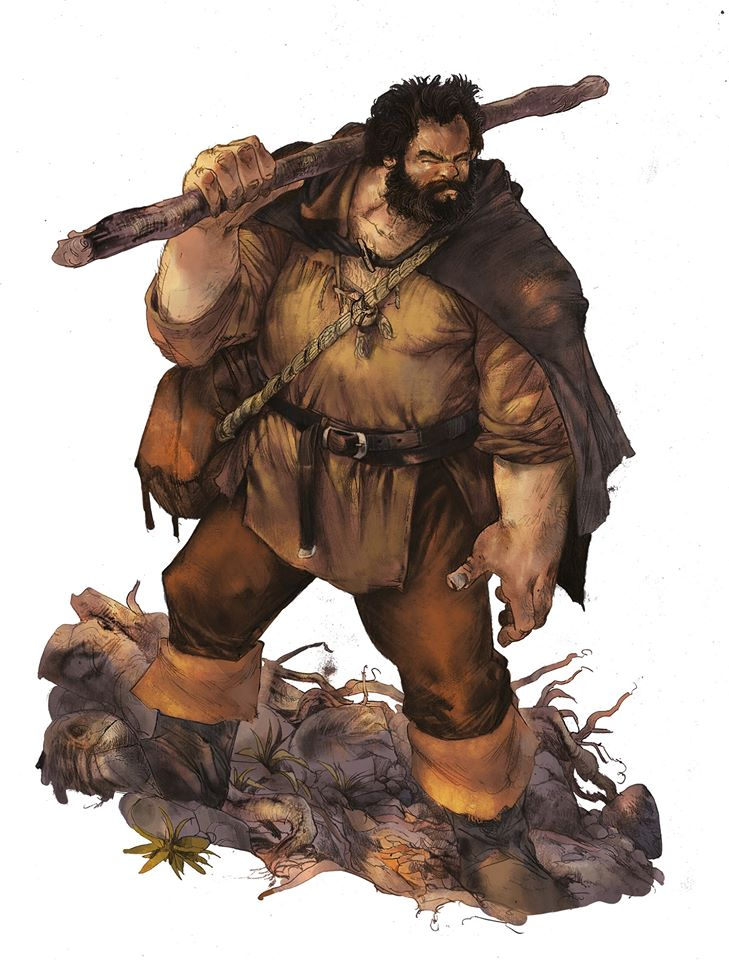
\includegraphics[width=0.48\textwidth]{04kins/img/19uman_monk.jpg}
\end{figure}

\subsection*{Traits}
    The nomad kin is known for their survival and adaptability, and your uman character receives the following traits:

    \subparagraph{Ability Score Increase} Two different ability scores of your choice are increased by 1.

    \subparagraph{Age} Umans reach adulthood in their late teens and live less than a century, if they manage to survive that long.

    \subparagraph{Alignment} Umans tend to no particular alignment, but they do have a penchant for community and justice, and tend to the indigo tide.

    \subparagraph{Size} Umans vary widely in height and build, from barely 1.5 meters to well over 1.8 meters tall.
    Regardless of your position in that range, your size is Medium.

    \subparagraph{Speed} Your base walking speed is 9 meters.

    \subparagraph{Languages} You can speak, read, and write the nomad tongue, and an additional language of your choice.
    You can also read and write the traveller's cant, a set of writings and symbols created by your kin to help and communicate with each other.

    \subparagraph{Learned Durability} You are competent in the Survival skill.

    \subparagraph{Relentless Endurance} When you are reduced to 0 hit points but not killed outright, you can drop to 1 hit points instead.
    You can't use this feature again until you finish a short rest.

    \subparagraph{Feats} From your kin, the feats available to you are
    \textbf{Alert} (page \pageref{feat::alert}),
    \textbf{Danger Sense} (page \pageref{feat::dangersense}),
    \textbf{Fleet of Foot} (page \pageref{feat::fleetoffoot}),
    \textbf{Last Resort} (page \pageref{feat::lastresort}),
    \textbf{Shadow Touched} (page \pageref{feat::shadowtouched}),
    \textbf{Tireless} (page \pageref{feat::tireless}), and
    \textbf{Uman Determination} (page \pageref{feat::umandetermination}).

\begin{figure}[!t]
    \centering
    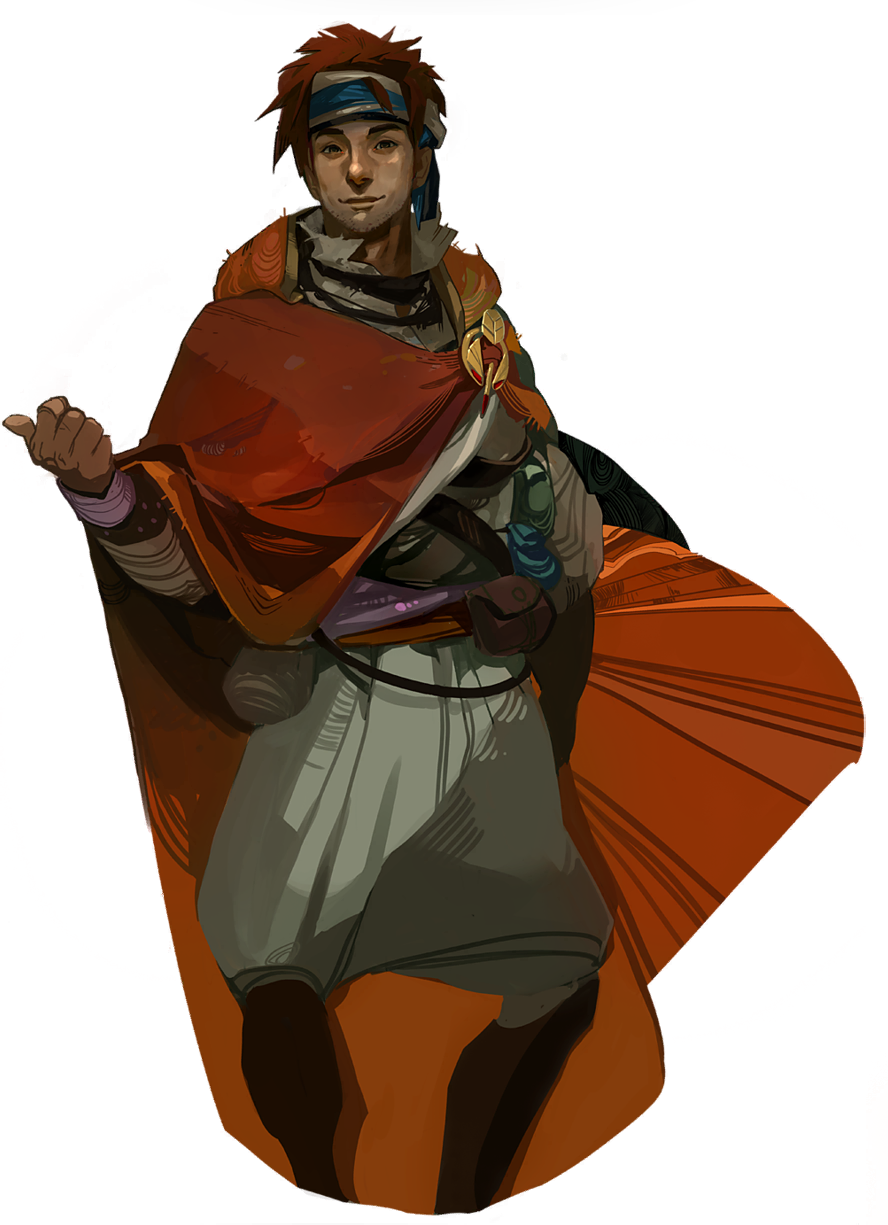
\includegraphics[width=0.48\textwidth]{04kins/img/19uman_nomad.png}
\end{figure}

\subsubsection{Common Uman}
    While umans are known to be extremely adaptable to extreme habitats, most don't stay at one place for enough time to acquire this specialty and remain, for lack of a better word, common.
    In stark contrast with their name, each of these umans is unique and as such your features are specially dynamic.

    \subparagraph{Languages} You can read, write and speak one additional language of your choice.

    \subparagraph{Skills} You are competent in one skill of your choice.

    \subparagraph{Trained} You are competent with simple weapons or one martial weapon type of your choice.

    \subparagraph{Handy} You are competent with a set of artisan's tools of your choice.

    \subparagraph{Feats} From your subrace, the feats available to you are
    \textbf{Adaptable} (page \pageref{feat::adaptable}),
    \textbf{Deft Hands} (page \pageref{feat::defthands}), and
    \textbf{Prodigy} (page \pageref{feat::prodigy}).

\subsubsection{Frostburn Nomad}
    With skins ranging from pale blue to light purple, and hair shades from the lightest of white to deep brown colors, the Frostburn are a kin that comes from a troupe of umans that managed to survive in the lands beyond the wall of ice and stone, and beyond the reach of most coldblood beasts and nimrods.
    % These umans tend to dress with the bones and furs of the creatures they hunt, using their inventiveness to craft clothing to intimidate and scare rather than protect against cold, since their thick skins already manage this task effortlessly.

    \subparagraph{Ability Score Increase} Your Constitution score is increased by 1.

    % \subparagraph{Menacing} You are competent in the Intimidation skill.

    \subparagraph{Born Hunter} You are competent with clubs, daggers, spears, and barbed weapons.
    During a long rest you can turn a dagger or spear into a barbed version of the weapon.
    When you succesfully attack a creature with a barbed weapon, the creature takes 1d4 necrotic damage at the beginning of its next turn.

    \subparagraph{Thick Skin} % You are naturally acclimated to cold environments and don't need sources of heat to survive in all but the most extreme cold.
    You are resistant to cold damage.%, and remain unaffected by cold environments.

    \subparagraph{Ice Shell} As two actions, you can grow a thick layer of ice around your body to protect you.
    You gain resistance to piercing and slashing damage and vulnerability to bludgeoning damage for a number of turns equal to your Constitution modifier (Minimum of 1).
    Additionally, any creature that attacks you with a melee attack during this time suffers 1d4 piercing damage.
    You can use this trait once per short rest.

    \subparagraph{Feats} From your subrace, the feats available to you are
    \textbf{Depths of Nerono} (page \pageref{feat::depthsofnerono}),
    \textbf{Impaling Carapace} (page \pageref{feat::impalingcarapace}), and
    \textbf{Thicker Skin} (page \pageref{feat::thickerskin}).

\subsubsection{Boggart}
    Boggarts are umans that live in the swamps and marshes of Yuadrem.
    Boggarts are generally tall, slim, and amber-skinned, with eyes of hazel or brown.
    Their hair ranges from black to dark brown, but most shave off all their hair.
    These umans are craftier than the average, and are known to prepare complex traps and mechanisms to protect their communities or alert them of imminent danger.

    \subparagraph{Ability Score Increase} Your Wisdom score is increased by 1.

    \subparagraph{Bog Swimmer} Boggart tactics usually include a good dose of swimming through less than cooperative waters.
    You have a swimming speed of 9 meters.

    \subparagraph{Swamp Life} You have advantage on saving throws against poison and diseases, and you have resistance against poison damage.

    \subparagraph{Stealthy Hunter} You are competent with blowguns, nets, and bolas.
    % You also are proficient with a Poisoner's kit.

    \subparagraph{Feats} From your subrace, the feats available to you are
    \textbf{Arboreal Alertness} (page \pageref{feat::arborealalertness}),
    \textbf{Keenest Senses} (page \pageref{feat::keenestsenses}), and
    \textbf{Primeval Awareness} (page \pageref{feat::primevalawareness}).

\subsubsection{Cursed Kin}
    It is said that the umans who remain in the place of their arrival start showing their true form.
    While the accuracy of this statement remains untested, it is true that those who stay in the forbidden lands do show strange changes to their appearance.
    Large, black horns grow on their heads, their skin and eyes turn into a very pale shade, and their bodies grow.
    While most cursed kin do act more menacing and violent than the average uman, it is likely that this is a side effect of their harsh homeland more than a natural development in their minds.

    \subparagraph{Size} Unlike most nomad kin, you stand between 2.1 and 2.4 meters tall and weight between 140 and 170 kg.
    Your size is medium.

    \subparagraph{Ability Score Increase} Your Strength score is increased by 1.

    % \subparagraph{Natural Athlete} You have proficiency in the Athletics skill.

    \subparagraph{Abyssal Resistance} You have resistance to fire damage.

    \subparagraph{Unholy Fortitude} Your hit point maximum increases by an amount equal to your level.

    \subparagraph{Ram} Your horns are a natural weapon, which you may use use to make unarmed strikes.
    If you hit with them, you deal bludgeoning damage equal to 1d4 + your Strength modifier, instead of the damage normal for an unarmed strike.

    \subparagraph{Powerful Build} You count as one size larger when determining your carrying capacity and the weight you can push, drag or lift.

    \subparagraph{Feats} From your subrace, the feats available to you are
    \textbf{Horned Fury} (page \pageref{feat::hornedfury}),
    \textbf{Imposing Presence} (page \pageref{feat::imposingpresence}), and
    \textbf{Savage Attacks} (page \pageref{feat::savageattacks}).

\begin{figure}[!b]
    \centering
    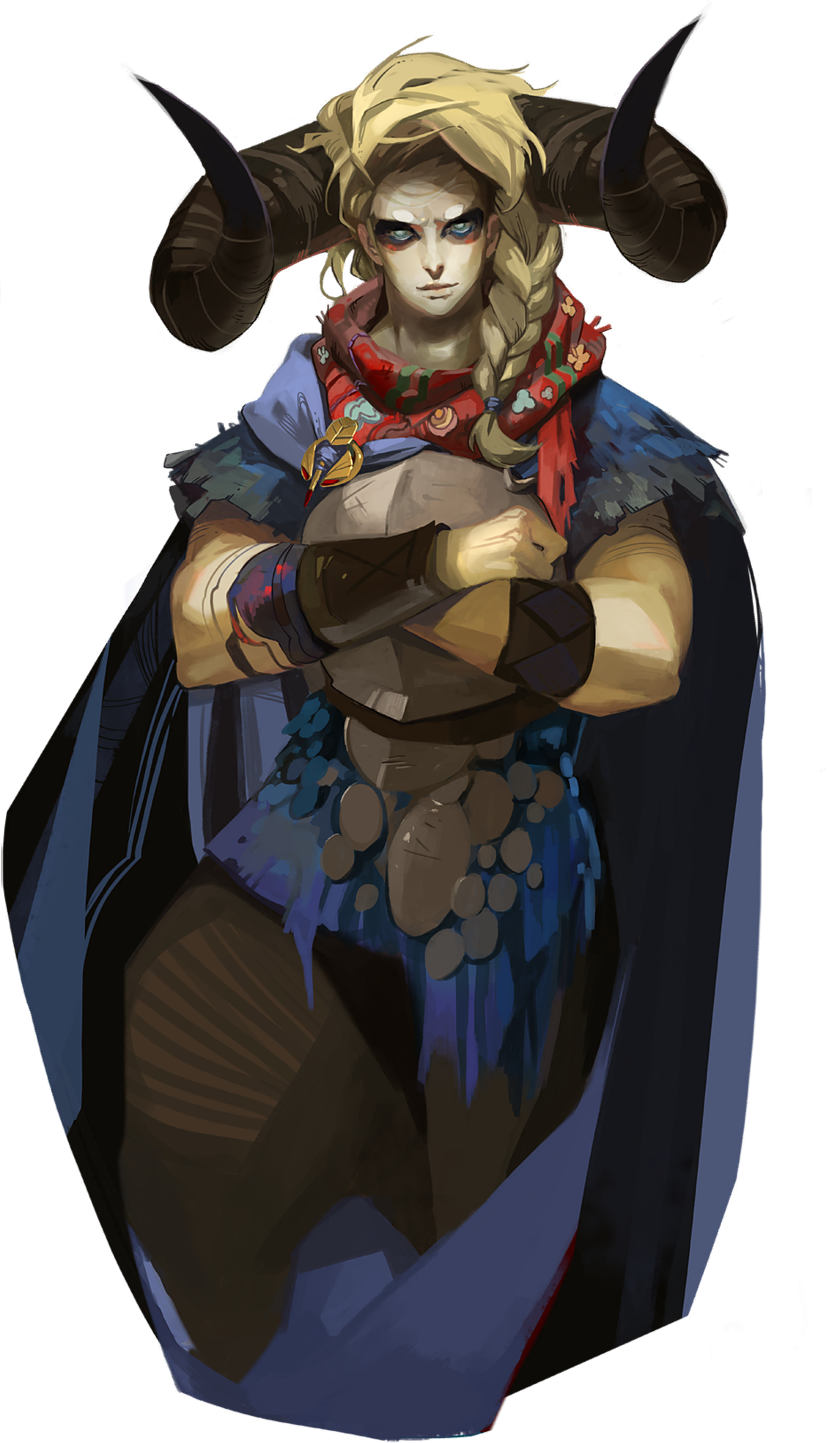
\includegraphics[width=0.48\textwidth]{04kins/img/19uman_cursed.png}
\end{figure}

% !TEX root = ../main.tex
\section{Storm Kin} \label{kin::zaloth}
\DndDropCapLine{A}{sk anyone anywhere and they will give}
\textit{you a list of the things and people they lost to the ash storm.
That blasted cloud covered the entirety of the continent, leaving none unscarred.}

\hspace*{\fill} --- Iitus the scholar, "Of War and Thunder".

As the schism progressed, when the spire started spewing forth smoke and lava into the world, an immense ash storm gathered around the volcano, discharging lightning into anyone foolish enough to approach it.
As the years passed, the storm slowly subsided, leaving behind a strange race of being composed of ash, smoke, and lightning.
These being were named the zaloths, or storm kin, who adapted surprisingly well to the many kins of Yuadrem, and quickly found their new place in the world.

\subsection*{Ethereal Appearance}
    The zaloths are tempests given physical shape, and their form reflects this.
    They are composed of ash smoke, with strange forces shaping them into humanoid form.
    Born from storm, they are in constant turmoil, and lightning sparks and cackles incessantly inside their bodies.

    It is social norm for zaloths to clothe themselves in linen wrappings to cover their bodies, and it is not unusual for them to wear clothes or armor over these wrappings.
    When they were formed, they also took the qualar of the unfortunate sentient creatures that were atop or near the spire, thus retaining their sentience.

    Zaloths are not known to age or reproduce, and as such it's hard to tell if they'll be able to survive too long as a species.
    They are thus extremely appreciative of their chance to experience life on Yuadrem, and are commonly known to be existentialists, looking to maximize their experiences in number and intensity.

    When a zaloth suffers a mortal wound it does not die in a traditional sense, but the matter composing its body coalesces into a zaloth quintessent, a small cloud of ash.
    This cloud does not retain its sentience, but it is somewhat able to keep its memories and experiences, and eventually merges into the atmosphere, becoming part of Yuadrem in a sense.

\subsection*{Distributed and Nomadic}
    While a small group of zaloths established themselves in the city of Jan'krug at the top of the spire, the vast majority of the storm kin immediately started roaming the world alone or in small groups, looking for experiences.
    Due to this, it is very rare to encounter an established zaloth community or zaloths living permanently in a city or town.
    Nowadays, they are found wondering the land in caravans, circuses or as lone adventurers, eternally seeking new experiences.

    When a wandering zaloth group meets another, it is common for them to celebrate this encounter by throwing a party in commemoration of their common heritage.
    During this event, the members of the different groups conduct a ritual known to them as the mingling, where they allow their bodies to fuse, and thus share with each other their memories and experiences.

\subsection*{Presence in the World}
    Due to their rarity, the other kins generally treat them with wonder and even admiration.
    Many schools of thought regard the zaloths as sages due to the wisdom obtained in their nomadic ways, and their unique viewpoint on life and the world is appreciated by any who seek knowledge.

    This however does not mean that all zaloths describe themselves as savant.
    On the contrary, some of them give in to their inherent chaotic nature and become agents of turmoil, seeking paramount experiences via extreme means.
    While their methods are frowned upon by more orthodox zaloths, they are far from being a pariah; they engage in mingling as commonly as any other zaloth.

\subsection*{Life of Adventure}
    Due to the existentialist nature of the zaloths, a life of adventure is the most natural lifestyle that comes to them.
    However, most zaloths are far from reckless, and while they can find dangers in their travels, they are careful to avoid mortal danger.
    To the storm kin, any zaloth's death is a tragedy, and they prioritize the life of any of their kin over that of all other creatures.

    A traveling zaloth will try all sorts of activities, independent of their nature and intensity.
    Ever seeking new experiences, it is equally likely to encounter a zaloth engaging in quiet appreciation of nature, martial combat against formidable enemies, or joining in on other species' religious rituals.
    Or even all of these activities on the same day.

\subsection*{Zaloth Names}
    Due to the special conditions to their coming into the world, zaloths are born without names.
    A zaloth usually chooses a name for itself after years, decades or even centuries of travel, and while it is nameless it is referred to using a feat or special characteristic that defines it.
    The names that a zaloth chooses are commonly taken from other cultures or carefully designed by it.

    \paragraph{Names}
    Basks-in-the-Sun, City-Swimmer, Dreams-of-Sleep, Dusk-Skin, Far-From-Water, Forest-Child, Has-no-Regrets, Head-in-Clouds, Iron-Fists, Mumbles-when-Speaks, Sees-All-Colors, Six-Coins, Somber-Mind, Sleeps-with-Open-eyes, Stands-in-Shallows, Swift-Legs, Takes-in-Light.

\begin{figure}[!t]
    \centering
    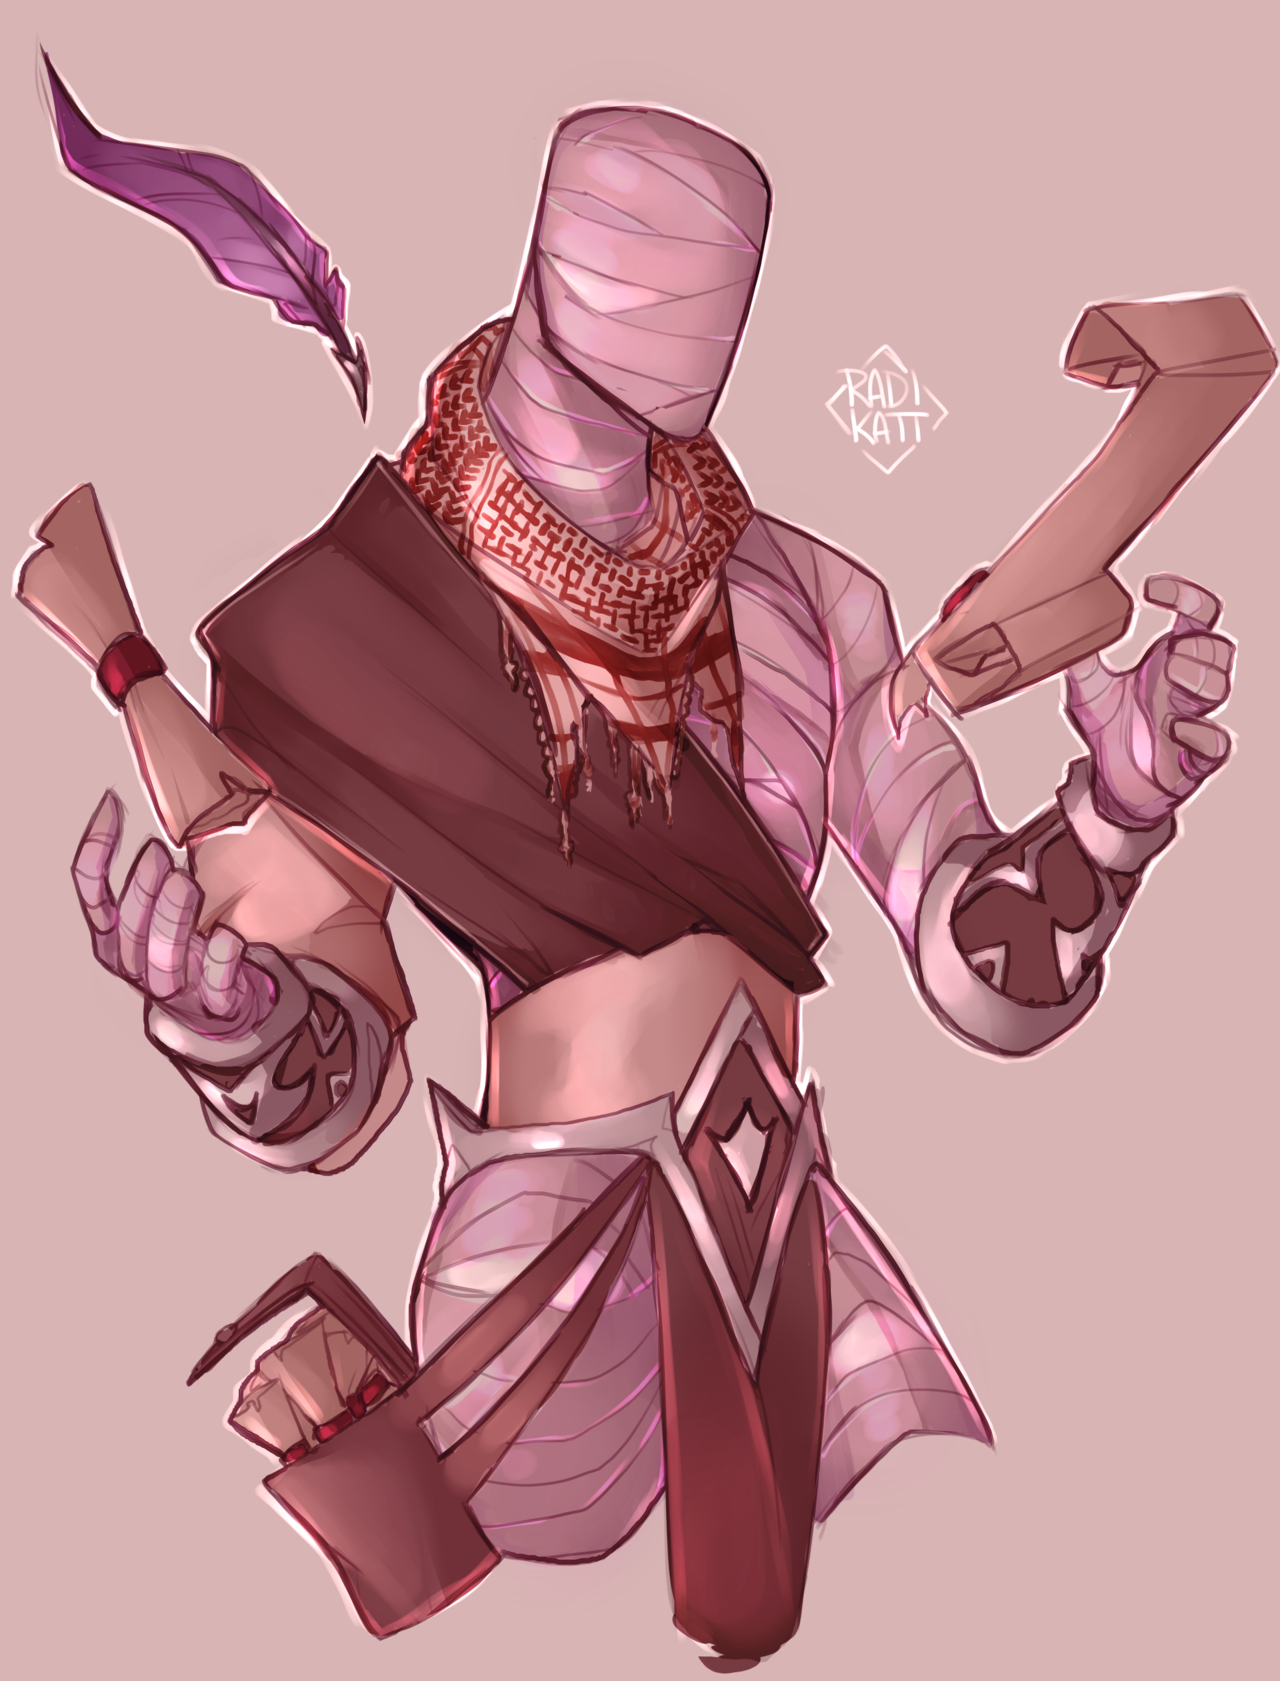
\includegraphics[width=0.48\textwidth]{04kins/img/20zaloth_scholar.png}
\end{figure}

\subsection*{Traits}
    Your zaloth character has an assortment of traits related to its unique nature and nomadic lifestyle.

    \subparagraph{Ability Score Increase} Your Charisma score increases by 1, and your Intelligence score increases by 1.

    \subparagraph{Age} Born from an ash storm, a zaloth is thrust into adulthood, retaining some of the memories of the tall one from which it acquired its qualar as a blurry image.
    Zaloths are not known to die from natural causes, and all of them are about 673 years old.

    \subparagraph{Alignment} Most zaloth tend toward chaos, with little regard for the affairs of civilizations.
    Due to their curious nature and lifestyle, zaloths move with the red tide.

    \subparagraph{Size} Zaloths stand between 1.5 and 1.8 meters, and are practically weightless due to their unique composition.

    \subparagraph{Speed} Your base walking speed is 9 meters.

    \subparagraph{Dual Nature} You are both humanoid and elemental.
    You can be affected by an effect if it works on either of these two creature types.

    \subparagraph{Incorporeal} You are immune to poison damage, and cannot be affected by poison or disease.
    Additionally, you don't need to eat or drink.

    % \subparagraph{Hover} Instead of walking, your can choose to hover up to 1 feet over the ground.
    % You can still be thrown into the ground if you are knocked prone, but you only need 5 feet of movement to stand up and don't provoke attacks of opportunity when you do so.

    \subparagraph{Radiant} You give off dim light in a 3-meter radius and have disadvantage on Dexterity (Stealth) checks.
    You cannot block this light with any clothing or armor.

    \subparagraph{Telepathic} You can speak telepathically to any creature you can see within 9 meters of you.
    Your telepathic utterances are in a language you know, and the creature understands you only if it knows that language.
    Your communication doesn't give the creature the ability to respond to you telepathically.

    \subparagraph{Silent Speaker} You can ignore the verbal components of spells.

    \subparagraph{Languages} You can understand, read and write two languages of your choice, but you are unable to speak.
    You can understand a very limited vocabulary of jantherlin, but your vocabulary consists of only individual words without context.

    \subparagraph{Feats} From your kin, the feats available to you are
    \textbf{Cosmic Omen} (page \pageref{feat::cosmicomen}),
    \textbf{Shadow Touched} (page \pageref{feat::shadowtouched}),
    \textbf{Starry Form} (page \pageref{feat::starryform}),
    \textbf{Stillness of Mind} (page \pageref{feat::stillnessofmind}),
    \textbf{Telekinetic} (page \pageref{feat::telekinetic}),
    \textbf{Telepathic} (page \pageref{feat::telepathic}), and
    \textbf{Zaloth Cunning} (page \pageref{feat::zalothcunning}).

\subsubsection{Gale Zaloth}
    Different zaloths have a stronger tendency towards different elements of the ash storm from which they were born.
    Gale zaloths are attuned to the shifting, violent winds of the storm, and they reflect this with their erratic movements and shifting conversation subjects.
    % A constant breeze can be felt around them, a grim reminder from the ash clouds.

    \subparagraph{Ability Score Improvement} Your Dexterity score increases by 1.

    \subparagraph{Stormbound} Wherever you go, you carry some of the storm with you.
    A light breeze can be permanently felt in a 3-meter radius around you, moving in a random direction every turn.
    The wind of this breeze displaces all smoke, gases, and very light objects inside its radius.
    You can choose to end or restart this effect as a free action.

    \subparagraph{Potent Quintessent} When you drop to 0 hit points, your desire to live manifests as a strong shockwave, sending any creature standing near you flying.
    All creatures that stands in a 3-meter radius around you must succeed on a DC of 12 + your Constitution modifier Strength saving throw.
    On a fail, a creature takes 1d6 force damage, is pushed 12 meters, and is knocked prone.
    On success, a creature only takes half the damage, and isn't pushed or knocked prone.
    You can use this ability once per short rest.

    \subparagraph{Wind Given Form} You know the gust cantrip.
    Once you gain your 3rd hit die, you can cast the feather fall spell.
    Once you gain your 5th hit die, you can cast the dust devil spell as a 2nd level spell, requiring no material components.
    Charisma is your spellcasting ability for these spells, and you can use each only once per short rest.

    \subparagraph{Feats} From your subrace, the feats available to you are
    \textbf{Fade Out} (page \pageref{feat::fadeout}),
    \textbf{Nimble Step} (page \pageref{feat::nimblestep}), and
    \textbf{One with the Wind} (page \pageref{feat::onewiththewind}).

\subsubsection{Thunder Zaloth}
    Thunder zaloths are attuned to the fleeting, fierce lightning.
    They reflect this relation with their quick movements and sparking personalities.

    \subparagraph{Ability Score Improvement} Your Charisma score increases by 1.

    \subparagraph{Instant Step} You can expend two actions to transport instantly to a location up to your movement speed away that you can see.
    Any creature standing in the straight line between the two positions must succeed on a DC 8 + your Constitution modifier Dexterity saving throw, taking 1d8 lightning damage on a failure.
    You can do this a number of times equal to your Charisma modifier (Minimum of 1), and regain all expended uses when you complete a short rest.

    \subparagraph{Elemental Resistance} You have resistance to lightning damage.

    \subparagraph{Electricity Given Form} You know the shocking grasp cantrip.
    Once you gain your 3rd hit die, you can cast the thunderwave spell as a 2nd level spell.
    Once you gain your 5th hit die, you can cast the shatter spell as a 2nd level spell.
    Charisma is your spellcasting ability for these spells, and you can use them only once per short rest.

    \subparagraph{Feats} From your subrace, the feats available to you are
    \textbf{Displace Teleportation} (page \pageref{feat::displaceteleportation}),
    \textbf{Fast as Lightning} (page \pageref{feat::fastaslightning}), and
    \textbf{Supercharged} (page \pageref{feat::supercharged}).

\subsubsection{Ash Zaloth}
    Ash zaloths are attuned to the destructive force of the spire, given form in the ash storm.
    They embody the violence of the storm, and have affinity towards inflicting and receiving pain.

    \subparagraph{Ability Score Improvement} Your Strength score increases by 1.

    \subparagraph{Storm Conduit} The chaos of combat stirs your inner storm.
    Once per round, you can deal an extra 1d4 fire damage to one creature you hit with an unarmed strike or an attack made with a metal weapon.
    At 11th level, this damage increases to 2d4.
    % You can do this a number of times equal to your Charisma modifier (Minimum of 1), and you regain all expended uses when you complete a short rest.

    \subparagraph{Elemental Resistance} You have resistance to fire damage.

    \subparagraph{Flame Given Form} You know the produce flame cantrip.
    Once you gain your 3rd hit die, you can cast the burning hands spell as a 2nd level spell.
    Once you gain your 5th hit die, you can cast the Aganazzar's scorcher spell as a 2nd level spell.
    Charisma is your spellcasting ability for these spells, and you can cast them once per short rest.

    \subparagraph{Feats} From your subrace, the feats available to you are
    \textbf{Fade Out} (page \pageref{feat::fadeout}),
    \textbf{Flames of Tizerus} (page \pageref{feat::flamesoftizerus}), and
    \textbf{Superheated} (page \pageref{feat::superheated}).

\subsubsection{Hail Zaloth}
    Rarest of their species, the hail zaloths are the youngest of the zaloth, embodying the freezing hail into which the ash storm eventually decanted.
    While still existentialist, they approach their curiosity in a calmer fashion, preferring the stillness of nature to the rowdiness of civilized society.

    \subparagraph{Ability Score Improvement} You Wisdom score increases by 1.

    \subparagraph{Cryogenic Stillness} You can choose to temporarily freeze your entire body, granting you extreme resilience.
    As an action or reaction, you can instantly freeze, granting you immunity to slashing, piercing, and bludgeoning damage, apart from resistance to acid, force, lightning, necrotic, and thunder damage.
    You also gain vulnerability to fire damage.
    You are also affected by the slow spell (see page \pageref{spell::slow}) for the duration of this trait without the possibility to roll saving throws.
    You can maintain this effect for a number of turns equal to your Charisma modifier (minimum of 1), and must finish a short rest in order to use this trait again.

    \subparagraph{Elemental Resistance} You have resistance to cold damage.

    \subparagraph{Ice Given Form} You know the frostbite cantrip.
    Once you gain your 3rd hit die, you can cast the ice knife spell as a 2nd level spell.
    Once you gain your 5th hit die, you can cast the icy surface spell as a 2nd level spell.
    Charisma is your spellcasting ability for these spells, and you can use them only once per short rest.

    \subparagraph{Feats} From your subrace, the feats available to you are
    \textbf{Arctic Temperature} (page \pageref{feat::arctictemperature}),
    \textbf{Depths of Nerono} (page \pageref{feat::depthsofnerono}), and
    \textbf{Gelid Aura} (page \pageref{feat::gelidaura}).

\begin{figure}[!b]
    \centering
    \includegraphics[width=0.48\textwidth]{04kins/img/20zaloth_thunder.jpg}
\end{figure}

\newpage

% !TEX root = ../main.tex
\section{Retainer Kin} \label{kin::quies}
\DndDropCapLine{T}{hey are the last kin made by our}
\textit{creators, and as such are related to us gats, irds, and oths.
It is our duty to provide them the nourishing that our shared parents denied them.
They are, after all, our younger siblings.}

\hspace*{\fill} --- Kosmael, founder of the church of Jismuah.

After the schism, as the storm that covered the tall kin's tiding dispersed, many dark secrets were revealed.
Among these sins, the existence of the quies, or retainer kin, was of special note.
The retainer kin is a fully sentient species which, unlike the other created by the tall kin, was forced into servitude, unable to comprehend what it is to roam free or even the existence of a world outside of Jan'krug.

At some point after the tall kin secluded themselves in their mountaintop city, they decided to create this slave race to focus solely on their studies and rituals.
The quies, not understanding what freedom is, remained immersed in their tasks for centuries, continuing even after the tall ones vanished.
They continued in this meaningless loop until a gat expedition found them, still locked into servitude to their dead masters, and showed them a life unbound by chains.

\subsection*{Designed with a Purpose}
    Such as gats, irds, oths, and marsets, the quies were created by the tall kin.
    Unlike them, the quies were formed from a blend of organic and inorganic materials.
    Their bodies are made from a blend of flesh and wood, with root-like cords infused with strange fluids serving as muscles, wrapped around a framework of bone and flesh.

    Armored plates form a protective outer shell and reinforce joints.
    Quies' faces are simply a collection of holes located where sensory organs would normally be, but each has a custom made qualar mask integrated into this outer shell.
    These masks usually contain very intricate detail, and seem to be made with an almost ardent passion.

\subsection*{Functionalist at Heart}
    The quies were built to serve.
    For the first centuries of their existence, the retainer kin had a clearly defined function and were encouraged to focus purely on that role.
    While they now might have freedom, many still struggle both to find a place in the world and to relate to the creatures of it.

    The typical quies show little emotion.
    Many of them embrace a concrete purpose-such as protecting allies, completing a contract, or exploring a land --- and embrace this task as they once did.
    However, there are quies who delight in exploring their feelings, their freedom, and their relationships with others.
    The race was first welcome to Yuadrem by the church of Jismuah, and many embraced faith and mysticism, seeking higher purpose and deeper meaning.

\subsection*{Life of Subservience}
    The quies are the sentient beings that spent the most time living alongside the tall kin, and as such they are highly sought after by scholars studying them.
    While a quies can describe in great detail the daily life of a tall one, their subservient nature inhibited their curiosity.
    Not one quies is known that can recall the rituals performed by the tall kin, and most can't even tell anything about their masters other done the tasks they performed for them.

    Like the zaloths, the quies are unable to reproduce by any mean, which is probably by design.
    This, combined with the fact that their creators have almost completely disappeared from Yuadrem, makes their chances of survival as a species look very grim.
    This is countered however by the fact that, as their creators, quies don't seem to age at all.

\subsection*{New Beginnings}
    After leaving Jan'krug, the retainer kin had a very hard time adapting to the world.
    Some dedicate themselves to continuing their skill under a new patron, failing to leave behind their lives as servants.
    Others managed to learn independence, but could not abandon their craft, and became renowned artisans or merchants, being compared by many even to gat artisans.

    The quies that managed to completely break free from their bindings are regarded as special by the other members of their species, and they are met with both reverence and jealousy.
    These quies usually become adventurers, where they can blend their newfound curiosity with their armored bodies.
    Some take the plight of their kin into their hearts, and spend their lives trying to find the last remaining tall ones, aiming to learn how to create more of their own.

\subsection*{Quies Names}
    As far as is known, no tall one ever gave a name to a quies.
    Most of the retainer kin simply refer to themselves by their job, or by a name given to them by others.
    However, the quies that manage to escape their shackles and take a life of wandering are very appreciative of being given the freedom to pick their own names.
    Once chosen, a quies will guard their name with great jealousy, only sharing it with whom they trust the most.

    \paragraph{Names}
    Ba, Bal, Dreth, Eth, Feather, Fish, Gakn, Green, I, Jan, Loth, Risz, Seed, Sekru, Stand, Swim, Tis, Tlekeloo, Tlos, When, Yu, Zash.

% \begin{figure}[!t]
%     \centering
%     \includegraphics[width=0.48\textwidth]{04kins/img/21quies_druid.png}
% \end{figure}

\subsection*{Traits}
    Designed for efficiency, your quies character has the following traits:

    \subparagraph{Ability Score Increase} Your Constitution and Strength scores increase by 1.

    \subparagraph{Age} Every quies is somewhere between 670 and 890 years old, but their memories before the schism are vague and unreliable.
    Since they've shown no sign of deterioration over time, quies are assumed to be impervious to aging.

    \subparagraph{Alignment} Most quies take comfort in order and discipline, tending toward law and neutrality, but some have chosen a new morality based on the experiences of their independent life.
    They came as a blank slate, and do not tend to any particular tide as a species.

    \subparagraph{Size} Quies are of formidable size, standing between 1.8 and 2.25 meters tall.
    Your build is determined by your subrace.
    Your size is medium.

    \subparagraph{Speed} Your base walking speed is 6 meters.

    \subparagraph{Dual Nature} Due to your manufactured nature, you are both humanoid and construct.
    You can be affected by an effect if it works on either of these two creature types.

    \subparagraph{Quies Resilience} You were created with fortitude in mind.
    You have advantage on saving throws against being poisoned, and you have resistance to poison damage.

    \subparagraph{Integrated Protection} Your body has built-in defensive layers, which can be enhanced with armor:

    \begin{itemize}
        \item You gain a passive +1 to Armor Class.
        \item You can only don armor with which you have proficiency.
        To don armor, you must incorporate it into your body as part of a short rest, during which you remain in contact with the armor.
        To doff armor, you must spend 1 hour removing it.
        \item While you live, your armor can't be removed from your body against your will.
    \end{itemize}

    \subparagraph{Mountain Built} You are impervious to all effects related to altitudes up to 20,000 meters, including cold and lack of oxygen.

\subsubsection{Operative}
    You were designed with a certain specialized function in mind.
    You might be a carpenter, a cartographer, or an entertainer, to name a few possibilities.

    Operatives are the most common of the quies, yet each is of unique design.
    Your build is dependent on the task you were designed for, and you can be as light as 70 kg to as heavy as 150 kg.

    \subparagraph{Ability Score Increase} Any ability score of your choice increases by 1.

    \subparagraph{Integrated Tool} You are competent with one set of artisan's tools or one instrument of your choice.
    This tool or instrument is integrated into your body, and is related to what was your purpose when you lived in Jan'krug.
    You must have your hands free to use this integrated tool.

    \subparagraph{Specialized Design} You are competent with one skill of your choice.

\subsubsection{Juggernaut}
    While many ets were more than capable of dealing with heavy lifting, they designed this branch of quies for fulfilling these tasks in conditions less ideal for them, or simply to work in cooperation with them.
    Juggernauts have a large frame and powerful build, and can weigh up to 230 kg.
    % While these quies were not specifically designed to fight, they usually prove more than capable of melee combat.

    \subparagraph{Ability Score Increase} Your Strength score increases by 1.

    \subparagraph{Hard Fists} Your arms and fists are lined with obsidian, a specially hard stone from the higher parts of the spire.
    When you hit with an unarmed strike, you can deal 1d4 + your Strength modifier bludgeoning damage, instead of the normal damage for an unarmed strike.

    \subparagraph{Powerful Build} You count as one size larger when determining your carrying capacity and the weight you can push, drag, or lift.

% \begin{table*}[b]%
%     \begin{DndTable}[width=\linewidth]{X}
%         \includegraphics[width=0.98\textwidth]{04kins/img/21quies_executioner.jpg}
%     \end{DndTable}
% \end{table*}

\subsubsection{Slag Worker}
    Even with the adaptable form of the tall kin, not even them can survive the extreme heat of lava for long.
    Consequently, they created the slag workers, quies designed specifically for working inside volcanoes.
    Built to work under extreme pressure, the carapace of the slag workers is a thick layer made from rhyolite.
    While the rock deforms and contorts under lava, it completely blocks the quies from the liquid and its heat.
    % Even the qualar of these quies is infused with the rock, to completely isolate them from their environment.

    \subparagraph{Ability Score Increase} Your Constitution score increases by 1.

    \subparagraph{Heavy Plating} This trait replaces integrated protection.
    You are covered by a rhyolite armor of a light-pink and gray color, containing small vugs filled with obsidian and quartz.
    Your Armor Class is 17, and you have disadvantage of Dexterity (Stealth) checks.
    For all intends and purposes your natural armor is considered Heavy Armor, and it cannot be removed from your body in any way while you are alive.

    \subparagraph{Specialized Worker} You are resistant to fire damage.
    You are also able to enter bodies of lava or magma, sinking at a speed of 5 feet per turn and not suffering any damage while inside.
    For the purposes of moving, lava and magma counts as difficult terrain for you.
    You still need to breathe, and must follow the normal rules for holding your breath while submerged in the hot liquid.

    \subparagraph{Defensive Stance} If you have one hand free, you can choose to enter a defensive stance as an action.
    You add a +3 to your AC until the start of your next turn.


    % \chapter{Walk of Life}

\DndDropCapLine{A}{part from their kin, your character}
is naturally defined by additional characteristics, such as their origin, background, and profession.
They are an individual with their own walk of life in the vast lands of Yuadrem.
This chapter explores the details separating your character from their peers, such as their name and physical description, their personality and alignment, and their origin and background.


% !TEX root = ../main.tex
\section{Details}
\subsection*{Name}
    While your character's kin description in the previous chapter contains a list of common names, you are welcome to create your own.
    For this, you can use the names in that list as a rough guideline to understand how their naming conventions usually works.

    Also think about how your character obtained their name.
    Each kin's section provides some information about how it's common for a member of your kin to obtain a name.
    Consider if this applies to your character and think what your character thinks of their name.
    Are they proud of it or do they dislike its origin or meaning?

\subsection*{Sex}
    Most of the kins are genderless, and thus sex and gender don't really have relevance in most societies of Yuadrem.
    If you choose to make a character of one of the gendered kins, keep in mind that their place in society will be generally unaffected.

    With the exception of the qulbaba ird's feathers, your character's stats and characteristics are unaffected by their sex.

\subsection*{Height and Weight}
    Based on their kin, you can decide your character's height and weight using the information in the Kins chapter.
    You are encouraged to think of how your character's ability scores relate to these characteristics, or even how they may clash.

    As in the PHB, you can roll randomly using the Random Height and Weight table.
    The dice roll given in the Height Modifier column determines the character's extra height (in cm) beyond the base height.
    Then, the dice roll given in the Weight Modifier column determines the character's extra weight (in kg) beyond the base weight.

\begin{DndTable}[width=\linewidth, header=Random Height and Weight]{lp{0.7cm}p{1.2cm}p{0.7cm}p{1.2cm}}
    \textbf{Kin} & \textbf{Base Height} & \textbf{Height Modifier} & \textbf{Base Weight} & \textbf{Weight Modifier} \\
    Gat               & 120  & 1d10 $\times$ 3  &  40  & 1d20 $\times$ 1   \\
    Treb Gat          & 160  & 1d10 $\times$ 4  &  90  & 1d10 $\times$ 3   \\
    Ird               & 170  & 1d10 $\times$ 3  &  40  & 1d10 $\times$ 1   \\
    thulkraka Ird     & 170  & 1d10 $\times$ 3  &  60  & 1d20 $\times$ 1   \\
    Marset            &  70  & 1d10 $\times$ 3  &  18  &  1d4 $\times$ 1   \\
    Oth               & 130  & 1d10 $\times$ 5  &  40  & 1d10 $\times$ 1   \\
    Naenk             & \multicolumn{4}{l}{See Size in page \pageref{kin::naenk.size}} \\
    Tsanek            & 180  & 1d10 $\times$ 2  &  60  & 1d20 $\times$ 1   \\
    Tortle            & 150  & 1d10 $\times$ 3  & 200  & 1d20 $\times$ 3   \\
    Grung             &  75  & 1d10 $\times$ 3  &  18  &  1d4 $\times$ 1   \\
    Uman              & 150  & 1d10 $\times$ 4  &  50  & 1d10 $\times$ 3   \\
    Zaloth            & 150  & 1d10 $\times$ 3  & < 1  & -                 \\
    Quies Operative   & 180  & 1d10 $\times$ 5  &  70  & 1d20 $\times$ 4   \\
    Quies Juggernaut  & 180  & 1d10 $\times$ 5  & 200  & 1d10 $\times$ 3   \\
    Quies Slag Worker & 180  & 1d10 $\times$ 5  & 250  & 1d10 $\times$ 5
\end{DndTable}

\subsection*{Physical Characteristics}
    Apart from what you've already defined, you also choose your character's age and eye, hair, and skin color.
    Some characteristics specific to your character's kin are also customizable, like a gat's horns or an ird's feather patterns.

    To help set apart your character from the rest, consider also giving them an unusual or memorable physical characteristic, such as a scar, a limp, or a tattoo.
    Think about how your character acquired such a feature and the story they might tell to explain it.

\subsection*{Qualar}
    Most people keep their qualars hidden and unadulterated.
    Some, however, enjoy carving messages or drawings into theirs, so as to enjoy themselves or to be remembered by the next carrier of the bone artifact.
    A few even cut small dents into it to place gems or crystal windows into the tarry liquid hidden within.

    Bonecarvers capable of crafting artificial qualars usually cut them into a specific design so that people know who made them.
    These designs can take many forms, like simple geometrical shapes to fine trinkets with intricate shapes.
    It is usual that these qualars are more expensive than the ones made by Ctereth, and the finest ones are usually reserved only for the elite.

    You are free to choose a qualar that makes sense for your character within reason.
    Also consider the relation your character has with their qualar.
    Perhaps they treasure it as a reminder of a home now abandoned, or maybe they want to exchange it in the first available opportunity.

% \pagebreak
%
% \begin{tikzpicture}[remember picture,overlay]
%     \node[anchor=north, yshift=0.10cm] at (current page.north) {\includegraphics[width=\pdfpagewidth]{05background/img/10the_sorrow}};
% \end{tikzpicture}
%
% \vspace{6.5cm}

\subsection*{Tidal Alignment}
    To define your character's moral compass and the way they interact with the world, define one or two dominant tides for them.
    The phenomenon of the tides is described in page \pageref{ssec::tides}.

    Examples of people aligned to each tide follow.

    \subparagraph{Blue Tide} A philosopher obsessed with the pursuit of enlightenment.
        A monk seeking wisdom to pass off to their school.
        A shaman making decisions for their tribe using both reason and mysticism.

    \subparagraph{Red Tide} An artist looking for passionate experiences to portray.
        An adventurer defying dangers in search of action and emotion.
        A crusader on a zealous quest for their divinity of choice.

    \subparagraph{Silver Tide} A ranger traversing an unexplored forest to leave a mark on history.
        A bard seeking to influence others with their music.
        A knight performing glorious deeds to acquire fame.

    \subparagraph{Indigo Tide} A congressperson writing laws to improve equity in their nation.
        A judge executing impartial justice to improve society as a whole.
        A tyrant governing under the hood of the greater good.

    \subparagraph{Gold Tide} A philanthropist aiding communities with their wealth.
        A crime lord who cares for their community for their own gain.
        A priest aiding the locals to gain favor from their god.

    When defining your character's tidal alignment, always remember that the tides are associated to action, not intention.
    Even if your character is merely seeking power, if to attain it they perform noble actions for a faction they will still improve their alignment with the gold tide.

% \begin{table*}[b]%
%     \begin{DndTable}[width=\linewidth]{X}
%         \centering
%         \includegraphics[width=0.95\textwidth]{05background/img/tidal_sway_rendition.png} \
%         \centering \large{\textbf{Artist's Rendition of The Sorrow.}}
%     \end{DndTable}
% \end{table*}

% \pagebreak~
% \vspace{7cm}

\subsection*{Personal Characteristics}
    For additional personal characteristics, you can follow the guidelines in pages 123 and 124 in the PHB.
    You are not limited however to personality traits, ideals, bonds, and flaws.
    You can flavor things as you see fit, adding attributes such as prides, dark secrets, flairs, etc.

    Your character might take pride in their cooking even if they're not a professional chef.
    Or they may have stolen an ancient family artifact before leaving home for adventure, claiming to have inherited it normally.
    They may also be a particularly good juggler, and tend to juggle with stones when bored in a social situation.

    Your character sheet includes an area to write your character's personal characteristics, but you are welcome to use additional sheets if your you need more space.
    As advice, it's often a good idea to put at least as much thought into your character's characteristics as you put into their appearance.

% !TEX root = ../main.tex
\section{Background}
Due to the open-endedness of characters in Yuadrem (see page \pageref{sec::classlessdnd} for more details), backgrounds as they are defined in the official D\&D5e books are not compatible with this book.
An alternative is proposed, where your character's background complements their kin, giving them a unique feat, and benefits when learning feats related to their background.

To choose religions and learned languages, refer to their respective sections in pages \pageref{ssec::religions} and \pageref{ssec::languages}.
These are not complete lists by any means, but rather the most common in the civilized world. %, and you are welcome to talk with your DM about including religions and languages as they may seem fit in your campaign.

\pagebreak

% For your character's background, you can choose any from some of the official D\&D5e books which fit best with your character.
% The specific books from which you are welcome to pick a background are Acquisitions Incorporated, Ghosts of Saltmarsh, the Player's Handbook, Mythic Odysseys of Theros, and Tomb of Annihilation.

% The only change you need to apply is to convert any initial money to the local currency of the region where you're playing.
% To do this, convert the GP to the local currency using the currencies table in page \pageref{sec::currency} using the selling value.

\textbf{TODO: EXPLAIN THE MECHANICS}
% TODO: Consider giving PCs the possibility of learning feats from other background, with the restriction that it needs one additional FP. This plays into the dynamism in Yuadrem.
% TODO: For bonds, flaws, etc., check the PHB.

\subsection*{Acolyte} \label{ssec::acolyte}
    Clerics, cultists, fanatics, and priests all share a devotion to something larger to themselves.
    You have spent your life in the service of a temple to a specific god or pantheon of gods.
    You act as an intermediary between the realm of the holy and the mortal world, performing sacred rites and offering sacrifices in order to conduct worshipers into the presence of the divine.

    Choose a god, a pantheon of gods, or some other divine being, and work with your DM to detail the nature of your religious service.
    This god or pantheon may be from any religion as detailed in the religion section (see pages \pageref{ssec::therism} for Therism and \pageref{ssec::religions} for other common religions), or a deity from outside of these pantheons that works with your DM.

    Were you a lesser functionary in a temple, raised from childhood to assist the priests in the sacred rites?
    Or were you a high priest who suddenly experienced a call to serve your god in a different way?
    Perhaps you were the leader of a small cult outside of any established temple structure, or even an occult group that served a fiendish master that you now deny.

    % Acolytes are shaped by their experience in temples or other religious communities.
    % Their study of the history and tenets of their faith and their relationships to temples, shrines, or hierarchies affect their mannerisms and ideals.

    \subparagraph{Competences} Religion, plus your choice of two from among History, Performance, Persuasion, and a language of your choice.

    \subparagraph{Equipment} A holy symbol representative of your religion, a prayer book or prayer wheel, vestments associated with your role, and a set of common clothes.

    \subparagraph{Feats} From your background, the feats available to you are
    \textbf{Divine Healing} (page \pageref{feat::divinehealing}),
    \textbf{Divine Inspiration} (page \pageref{feat::divineinspiration}),
    \textbf{Guidance} (page \pageref{feat::guidance}),
    \textbf{Incite Respect} (page \pageref{feat::inciterespect}),
    \textbf{Inspiring Leader} (page \pageref{feat::inspiringleader}), and
    \textbf{Shelter of the Faithful} (page \pageref{feat::shelterofthefaithful}).

    \subsubsection{Voice of your God} \label{feat::voiceofyourgod}
        You are capable of performing any religious ceremony associated to your deity.
        You can do this in any established temple, improvised altar, or public plaza, and can expect to at least gather the attention of those around you.

        If you spend at least an hour performing this activity, you can choose to roll a Charisma (Performance) check contested against a target's --- or targets' --- Wisdom (Insight).
        On a success, they are charmed by you for 1d4 hours.
        This charm ends if you or one of your companions harms the creature.

        Additionally, you might receive a small donation for your performance at the DM's discretion.
    % ========================================================================== %

\subsection*{Artisan} \label{ssec::artisan}
    Crafters, guild artisans, inventors, and engineers all fall into this category.
    Either as part of a guild or a working solo, you are skilled in a particular field and are closely associated with other artisans.
    You are a well-established part of the mercantile world, freed by talent and wealth from the constraints of a feudal social order.
    You learned your skills as an apprentice to a master artisan, maybe under the sponsorship of a guild, until you became a master in your own right.

    \subparagraph{Competences} A set of artisan's tools of your choice, plus your choice of two from among Insight, Perception, Sleight of Hand, and another set of artisan's tools.

    \subparagraph{Equipment} A set of artisan's tools with which you are proficient, a maker's mark chisel used to mark your handiwork with the symbol of your guild, and a set of traveler's clothes.

    \subparagraph{Feats} From your background, the feats available to you are
    \textbf{Artificer's Infusions} (page \pageref{feat::artificersinfusion}),
    \textbf{Beyond Mastery} (page \pageref{feat::beyondmastery}),
    \textbf{Flash of Genius} (page \pageref{feat::flashofgenius}),
    \textbf{Guild Membership} (page \pageref{feat::guildmembership}),
    \textbf{Known Crafter} (page \pageref{feat::knowncrafter}), and
    \textbf{The Right Tool for the Job} (page \pageref{feat::therighttoolforthejob}).

    \subsubsection{Cunning Artisan} \label{feat::cunningartisan}
        As part of a short rest, you can harvest materials from the wilds, the city, or a slain beast of size small or larger to create one of the following items: a shield, a club, a javelin, or 1d4 darts or blowgun needles.
        To use this trait, you need a blade, such as a dagger, or appropiate artisan's tools, such as leatherworker's tools.
    % ========================================================================== %

\subsection*{Criminal} \label{ssec::criminal}
    Bandits, pirates, spies, and thieves all share a penchant for crime.
    You are an experienced criminal with a history of breaking the law.
    You have spent a lot of time among other criminals and still have contacts within the criminal underworld.
    You're far closer than most people to the world of murder, theft, and violence that pervades the underbelly of civilization, and you have survived up to this point by flouting the rules and regulations of society.

    There are many kinds of criminals, and within a thieves' guild or similar criminal organization, individual members have particular specialties.
    Even criminals who operate outside of such organizations have strong preferences for certain kinds of crimes over others.
    Choose the role you played in your criminal life.

    \subparagraph{Competences} Deception, plus your choice of two from among Intimidation, Sleight of Hand, Stealth, or a set of Thieves' Tools.

    \subparagraph{Equipment} A crowbar, a black cloak with a hood, a set of dark common clothes, and a knife.

    \subparagraph{Feats} From your background, the feats available to you are
    \textbf{Cunning Action} (page \pageref{feat::cunningaction}),
    \textbf{Criminal Contact} (page \pageref{feat::criminalcontact}),
    \textbf{Down Low} (page \pageref{feat::downlow}),
    \textbf{Dual Personalities} (page \pageref{feat::dualpersonalities}),
    \textbf{Undecity Paths} (page \pageref{feat::undercitypaths}), and
    \textbf{Urban Infrastructure} (page \pageref{feat::urbaninfrastructure}).

    \subsubsection{Thieves' Cant} \label{feat::thievescant}
        You know Thieves' cant, a secret mix of dialect, jargon, and code that allows you to hide messages in seemingly normal conversation.
        Only another creature that knows thieves' cant understands such messages.
        It takes four times longer to convey such a message that it does to speak the same idea plainly.

        In addition, you understand a set of secret signs and symbols used to convey short, simple messages, such as whether an area is dangerous or the territory of a thieves' guild, whether loot is nearby, or whether the people in an area are easy marks or will provide a safe house for thieves on the run.
    % ========================================================================== %

\subsection*{Entertainer} \label{ssec::entertainer}
    Acrobats, athletes, gladiators, and performers all share a passion for self-improvement, their art, and entertainment. % Considering athletes here is a bit shit but is the best I can do tbh.
    You thrive in front of an audience.
    You know how to entrance them, entertain them, and even inspire them.
    Whatever techniques you use, your art is your life.

    \subparagraph{Competences} Performance, plus your choice of two from among Acrobatics, Athletics, a musical instrument, or land vehicles.

    \subparagraph{Equipment} A tool related to your art (a musical instrument, a weapon, a leather ball, etc.), a lucky charm or past trophy, and costume clothes.

    \subparagraph{Feats} From your background, the feats available to you are
    \textbf{Bardic Inspiration} (page \pageref{feat::bardicinspiration}),
    \textbf{Courtier} (page \pageref{feat::courtier}),
    \textbf{Jack of All Trades} (page \pageref{feat::jackofalltrades}),
    \textbf{Rakish Audacity} (page \pageref{feat::rakishaudacity}),
    \textbf{Rustic Hospitality} (page \pageref{feat::rustichospitality}), and
    \textbf{Song of Rest} (page \pageref{feat::songofrest}).

    \subsubsection{By Popular Demand} \label{feat::bypopulardemand}
        You can always find a place to perform, may it be an inn, a tavern, an arena, a field, or even in a noble's court.
        At such a place, you receive free lodging and food of a modest or comfortable standard (depending on the quality of the establishment), as long as you perform daily.
        In addition, your performance makes you something of a local figure.
        When strangers recognize you in a town where you have performed, they typically take a liking to you.
    % ========================================================================== %

\subsection*{Laborer} \label{ssec::laborer}
    Born a laborer, you have jumped through one odd job to the next through your entire life.
    One day you might be a farmhand, another a miner, then a servant, and later a stevedore.
    You adapt as is required, with a sharp nose for coin.

    You have dirt under your fingernails and never shy away from a little hard work.
    Most of your time is filled in back-breaking labor, the type of work that keeps merchants and mine owners in business even as it makes you just enough money to get by.
    It’s a hard life, but it’s toughened you and made you confident in your abilities.

    \subparagraph{Competences} Athletics, plus your choice of two from among Animal Handling, Survival, land vehicles, or a set of artisan's tools of your choice.

    \subparagraph{Equipment} A job-related tool (choose a piece of equipment that costs 2 agnomas or less), small knife, a set of bone dice or a deck of Huathem cards, and a set of common clothes.

    \subparagraph{Feats} From your background, the feats available to you are
    \textbf{Commoner's Toughness} (page \pageref{feat::commonerstoughness}),
    \textbf{Deep Miner} (page \pageref{feat::deepminer}),
    \textbf{Powerful Build} (page \pageref{feat::powerfulbuild}),
    \textbf{Resilient} (page \pageref{feat::resilient}),
    \textbf{Rustic Hospitality} (page \pageref{feat::rustichospitality}), and
    \textbf{Urban Infrastructure} (page \pageref{feat::urbaninfrastructure}).

    \subsubsection{Hired Hand}
        As one of the working class, finding work and a place to stay is easy for you.
        In any location that needs workers, you can find room and board for you and your companions.
        You also get enough money for a poor lifestyle for as long as the work holds out, unless you or your companions prove to be a danger to those around you.
        Your employer and the other laborers may even protect you from the law or anyone else searching for you, though they will not risk their lives for you.
    % ========================================================================== %

\subsection*{Merchant} \label{ssec::merchant}
    Caravan masters, shopkeepers, and traders all focus on one thing: coin.
    You don't craft items yourself but earn a living by buying and selling the works of others (or the raw materials artisans need to practice their craft).
    You might be part of a large merchant consortium or family with interests across the region. Perhaps you transported goods from one place to another, by ship, wagon, or caravan, or bought them from traveling traders and sold them in your own little shop.

    \subparagraph{Competences} Persuasion, plus your choice of two from among Investigation, a set of navigator's tools, one language, or land vehicles.

    \subparagraph{Equipment} A mule and cart, a merchant's scale, a set of fine clothes, and a belt containing 10 agnomas (nickel coins, see page \pageref{sec::currency}).

    \subparagraph{Feats} From your background, the feats available to you are
    \textbf{Down Low} (page \pageref{feat::downlow}),
    \textbf{Guild Membership} (page \pageref{feat::guildmembership}),
    \textbf{Master Negotiator} (page \pageref{feat::masternegotiator}),
    \textbf{Never Tell Met he Odds} (page \pageref{feat::nevertellmetheodds}),
    \textbf{Silver Tongue} (page \pageref{feat::silvertongue}), and
    \textbf{Unsettling Words} (page \pageref{feat::unsettlingwords}).

    \subsubsection{Supply Chain} \label{feat::supplychain}
        From your time as a merchant, you retain connections with wholesalers, suppliers, and other merchants and entrepreneurs.
        You can call upon these connections when looking for items or information.
        In locations where you are not familiar, you are able to establish this web of connections as part of a long rest.
    % ========================================================================== %

\subsection*{Noble} \label{ssec::noble}
    You understand wealth, power, and privilege.
    You carry a noble title, and your family owns land, collects taxes, and wields significant political influence.
    You might be a pampered aristocrat unfamiliar with work or discomfort, a former merchant just elevated to the nobility, or a champion who gained status via knighthood.
    Or you could be an honest, hard-working landowner who cares deeply about the people who live and work on your land, keenly aware of your responsibility to them.

    \subparagraph{Competences} History, plus your choice of two from among Deception, Persuasion, Religion, or a language of your choice.

    \subparagraph{Equipment} A set of fine clothes, and signet ring with your family's sigil, and a purse containing 25 agnomas.

    \subparagraph{Feats} From your background, the feats available to you are
    \textbf{Courtier} (page \pageref{feat::courtier}),
    \textbf{Early Training} (page \pageref{feat::earlytraining}),
    \textbf{Kept in Style} (page \pageref{feat::keptinstyle}),
    \textbf{Legalese} (page \pageref{feat::legalese}),
    \textbf{Promise of Status} (page \pageref{feat::promiseofstatus}), and
    \textbf{Retainers} (page \pageref{feat::retainers}).

    \subsubsection{Position of Priviledge}
        Thanks to your noble birth, people are inclined to think the best of you.
        You are welcome in high society, and people assume you have the right to be wherever you are.
        The common folk make every effort to accommodate you and avoid your displeasure, and other people of high birth treat you as a member of the same social sphere.
        You can secure an audience with a local noble if you need to.

        You can exert leverage over one or more individuals below you in the social hierarchy and demand their help as needs warrant.
        For example, you can have a message carried across a neighborhood, procure a short carriage ride without paying, or have others clean up a bloody mess you left in an alley.
        The DM decides if your demands are reasonable and if there are people available and willing to fulfill them.
        As your social status improves, you gain influence over more people, including ones in greater positions of power.
    % ========================================================================== %

\subsection*{Sailor} \label{ssec::sailor}
    You sailed on a seagoing vessel for years.
    In that time, you faced down mighty storms, monsters of the deep, and those who wanted to sink your craft to the bottomless depths.
    Your first love is the distant line of the horizon.

    Discuss the nature of the ship you previously sailed with your Dungeon Master.
    Was it a merchant ship, a naval vessel, a ship of discovery, or a pirate ship?
    How famous (or infamous) is it?
    Is it widely traveled?
    Is it still sailing, or is it missing and presumed lost with all hands?
    What were your duties on board?

    \subparagraph{Competences} Water vehicles, plus your choice of two from among Perception, Survival, Navigator's Tools, or Carpenter's Tools.

    \subparagraph{Equipment} A belaying pin, 50 feet of silk rope, a lucky charm, and a set of common clothes.

    \subparagraph{Feats} From your background, the feats available to you are
    \textbf{Drunken Resilience} (page \pageref{feat::drunkenresilience}),
    \textbf{Expert Stirrer} (page \pageref{feat::expertstirrer}),
    \textbf{Harvest the Water} (page \pageref{feat::harvestthewater}),
    \textbf{I'll Patch It} (page \pageref{feat::illpatchit}),
    \textbf{Sailor's Balance} (page \pageref{feat::sailorsbalance}), and
    \textbf{Wisdom of the Wilds} (page \pageref{feat::wisdomofthewilds}).

    \subsubsection{Ship's Passage}
        When you need to, you can secure free passage on a sailing ship for yourself and your companions.
        You might sail on the ship you served on, or another ship you have good relations with (perhaps one captained by a former crewmate).
        Because you're calling in a favor, you can't be certain of a schedule or route that will meet your every need.
        Your Dungeon Master will determine how long it takes to get where you need to go.
        In return for your free passage, you and your companions are expected to assist the crew during the voyage.
    % ========================================================================== %

\subsection*{Scholar} \label{ssec::scholar}
    Sages, scholars, students, and scientists are all passionate about one or many fields of study.
    You are defined by your extensive studies, and your characteristics reflect this life of study.
    Devoted to scholarly pursuits, you value knowledge highly --- sometimes in its own right, sometimes as a means toward other ideals.

    \subparagraph{Competences} Investigation, plus your choice of two from among Arcana, History, Medicine, or one language.

    \subparagraph{Equipment} A bottle of black ink, a quill, a small knife, a letter from a dead colleague posing a question you have not yet been able to answer, and a set of common clothes.

    \subparagraph{Feats} From your background, the feats available to you are
    \textbf{Adept Linguist} (page \pageref{feat::adeptlinguist}),
    \textbf{Flash of Genius} (page \pageref{feat::flashofgenius}),
    \textbf{Historical Knowledge} (page \pageref{feat::historicalknowledge}),
    \textbf{Legalese} (page \pageref{feat::legalese}),
    \textbf{Metamagic Adept} (page \pageref{feat::metamagicadept}), and
    \textbf{Skill Versatility} (page \pageref{feat::skillversatility}).

    \subsubsection{Researcher} \label{feat::researcher}
        When you attempt to learn or recall a piece of lore, if you do not know that information, you often know where and from whom you can obtain it.
        Usually, this information comes from a library, scriptorium, university, or a sage or other learned person or creature.
        Your DM might rule that the knowledge you seek is secreted away in an almost inaccessible place, or that it simply cannot be found.
    % ========================================================================== %

\subsection*{Soldier} \label{ssec::soldier}
    You trained as a youth, studied the use of weapons and armor, learned basic survival techniques, including how to stay alive on the battlefield.
    You might have been part of a standing army or a mercenary company, or perhaps a member of a local militia who rose to prominence during a recent war.

    When you choose this background, work with your DM to determine which military organization you were a part of, how far through its ranks you progressed, and what kind of experiences you had during your military career.
    Was it a standing army, a town guard, or a village militia?
    Or it might have been a noble's order of knights, a merchant's private army, or a mercenary company.

    \subparagraph{Competences} Competence with a weapon type of your choice, plus your choice of two from among Athletics, Intimidation, an armor type of your choice, or land vehicles.

    \subparagraph{Equipment} An insignia of rank, a trophy taken from a fallen enemy, and a set of common clothes.

    \subparagraph{Feats} From your background, the feats available to you are
    \textbf{} (page \pageref{feat::}),
    \textbf{} (page \pageref{feat::}),
    \textbf{} (page \pageref{feat::}),
    \textbf{} (page \pageref{feat::}),
    \textbf{} (page \pageref{feat::}), and
    \textbf{} (page \pageref{feat::}).

    \subsubsection{Military Rank}
        You have a military rank from your career as a soldier.
        Soldiers loyal to your former military organization still recognize your authority and influence, and they defer to you if they are of a lower rank.
        You can invoke your rank to exert influence over other soldiers and requisition simple equipment or horses for temporary use.
        You can also usually gain access to friendly military encampments and fortresses where your rank is recognized.
    % ========================================================================== %

\subsection*{Outlander} \label{ssec::outlander}
    Either by choice or by birthright, you have spent much of your life in the wilds, far from the comforts of civilization.
    You've witnessed the migration of herds larger than forests, survived weather more extreme than any city-dweller could comprehend, and enjoyed the solitude of being the only thinking creature for miles in any direction.
    The wilds are in your blood, whether you were a nomad, an explorer, a recluse, a hunter-gatherer, or a hermit.
    Even in places where you don't know the specific features of the terrain, you know the ways of the wild.

    \subparagraph{Competences} Survival, plus your choice of two from among Animal Handling, Athletics, Nature, or a musical instrument.

    \subparagraph{Equipment} A staff, a hunting trap, a trophy from an animal you killed, and a set of traveler's clothes.

    \subparagraph{Feats} From your background, the feats available to you are
    \textbf{} (page \pageref{feat::}),
    \textbf{} (page \pageref{feat::}),
    \textbf{} (page \pageref{feat::}),
    \textbf{} (page \pageref{feat::}),
    \textbf{} (page \pageref{feat::}), and
    \textbf{} (page \pageref{feat::}).

    \subsubsection{Wanderer}
        You have an excellent memory for maps and geography, and you can always recall the general layout of terrain, settlements, and other features around you.
        In addition, you can find food and fresh water for yourself and up to five other people each day, provided that the land offers berries, small game, water, and so forth.
    % ========================================================================== %

% Strength
%     !3 Athletics
% Dexterity
%     .1 Acrobatics
%     .2 Sleight of Hand
%     .1 Stealth
% Intelligence
%     .1 Arcana
%     !2 History
%     !1 Investigation
%     .1 Nature
%     !1 Religion
% Wisdom
%     .2 Animal Handling
%     .2 Insight
%     .1 Medicine
%     .2 Perception
%     !2 Survival
% Charisma
%     !1 Deception
%     .2 Intimidation
%     !1 Performance
%     !2 Persuasion
% !0 Weapon
% .1 Armor
% !6 Tools
% .2 Instrument
% .4 Languages
% .4 Vehicles (land)
% !0 Vehicles (water)
% .0 Vehicles (air)

\section{Origins}

\DndDropCapLine{I}{n Yuadrem, your character's mother}
language and some common characteristics may be defined by their country of origin.
While not too much detail is given per country, you are welcome to speak with your DM (or the book's author!) if you need more information about a specific one.

To help you decide a country of origin or let a die roll decide it, a political map and a table of countries are given.
The table lists all countries with their common kins, common languages, and some cultural mannerisms.

The \textbf{common kin(s)} column simply represents the kin of the people you're most likely to come into when in a city, but is not an exhaustive list.

\begin{table*}[b]%
    \begin{DndTable}[width=\linewidth]{X}
        \centering
        \includegraphics[width=0.95\textwidth]{05background/img/king_of_the_gray_sands_trebos.jpg} \
        \centering \large{\textbf{Trebos, King of the Gray Sands}}
    \end{DndTable}
\end{table*}

Then, the \textbf{common language(s)} column represents the most spoken (or official) language in the country, while the second or third languages in the column are commonly heard tongues among the people.

Finally, the \textbf{cultural mannerisms} column is a list of common stereotypes associated to the people of a country.
While they are not necessarily true for each particular person, your character might pride themselves or react in a certain manner to the specific characteristics attributed to their country of origin.

It's worth noting that there are six areas shown in the political map and described in the table are not exactly countries in a traditional sense, but are well-defined regions of land where for one reason or another no culture has declared their own.

The first of these is Jatuunsa, the land of the giants.
Then Nastralinal, the land of the ettins.
The Nest, home to the mysterious Fo.
The majority of the Wildlands, inhabited by the tidal creatures.
The Wurmlands, home to the wurm colonies.
And Zashlath, the insurmountable desert.

While not official countries in any degree, some nomad tribes and a few permanent settlements exist in these untamed lands, and you are more than welcome to make one of these the birthplace of your character.

If you want to let the dice decide your character's origin, roll a d6 and a d20 and use the results.
The first table in the list represents the dice rolls, in a d6,d20 format.

If the d6 lands on a 6 and the d20 on a 18, 19, or 20, you can always make your character be a late arrival.
Late arrivals can either be umans, tortles, or grungs ``coming late'' from the Sizzling Gate, or zaloth and quies that for any reason didn't join their kin after the schism.

\incgraph[documentpaper,][width=\paperwidth,height=\paperheight]{05background/img/political_map.png}

\begin{table*}[!ht]%
    \begin{DndTable}[width=\linewidth, header=Country List]{p{0.65cm}p{3cm}XXX}
        \textbf{Die} & \textbf{Country}           & \textbf{Common kin(s)}               & \textbf{Common Language(s)}  & \textbf{Cultural Mannerism(s)}  \\
        1, 1             & \textbf{Abababa}           & marset                               & Babazano                     & distrustful                     \\
        1, 2             & \textbf{Abipolash}         & moonborn \& chu’ash oth              & Shamabic, Fruenese           & resentful, careful              \\
        1, 3             & \textbf{Adraman}           & chu’ash oth                          & Shamabic                     & rude, defensive                 \\
        1, 4             & \textbf{Babana}            & marset, tortle                       & Babazano, Krelho             & protective, welcoming           \\
        1, 5             & \textbf{Barit}             & cliff \& bughna gat, zsek ird        & Avshenese, Zsekian           & business-minded, greedy         \\
        1, 6             & \textbf{Beilios}           & chu’ash oth                          & Shamabic                     & unwelcoming                     \\
        1, 7             & \textbf{Brovish}           & bughna gat                           & Avshenese                    & uncivilized, competitive        \\
        1, 8             & \textbf{Byurev}            & cliff \& bughna gat                  & Avshenese                    & defensive, decisive             \\
        1, 9             & \textbf{Cabb Goem Rlamesh} & varied                               & Conscript Tongue             & strange, secretive              \\
        1, 10            & \textbf{Chitsia}           & varied                               & Fruenese                     & remorseful, distrustful         \\
        1, 11            & \textbf{Dentralin}         & qulbaba ird                          & Qualinese                    & traditionalist, disciplined     \\
        1, 12            & \textbf{Diathal}           & qulbaba ird                          & Qualinese                    & defensive, indifferent          \\
        1, 13            & \textbf{Digmis}            & cliff \& bughna gat                  & Avshenese                    & resourceful                     \\
        1, 14            & \textbf{Dnimas}            & treb gat, zsek ird                   & Avshenese, Zsekian           & traditional, conniving          \\
        1, 15            & \textbf{Dnomit}            & cliff gat                            & Avshenese                    & faint-hearted, broad-minded     \\
        1, 16            & \textbf{Drer}              & varied                               & Fruenese                     & impulsive, creative             \\
        1, 17            & \textbf{Dzarog}            & treb gat, cursed uman                & Avshenese, Jantherlin        & mysterious, calm                \\
        1, 18            & \textbf{Dzokrenar}         & thulkraka \& zsek ird                & Harualish, Zsekian           & religious, traditionalist       \\
        1, 19            & \textbf{Edede}             & marset                               & Babazano                     & distrustful, protective         \\
        1, 20            & \textbf{Erpat}             & bughna gat                           & Avshenese                    & curious, aggressive             \\
        2, 1             & \textbf{Esketis}           & cliff gat, thulkraka ird             & Shanise, Avshenese           & distrustful                     \\
        2, 2             & \textbf{Faros}             & chu’ash oth                          & Shamabic                     & carefree                        \\
        2, 3             & \textbf{Fobros}            & bughna gat                           & Avshenese                    & hardworking, violent            \\
        2, 4             & \textbf{Folhoghit}         & cliff gat, thulkraka ird             & Avshenese                    & traditionalist, business-minded \\
        2, 5             & \textbf{Fraid}             & chu’ash oth, zsek ird                & Shamabic, Zsekian            & friendly, trusting              \\
        2, 6             & \textbf{Froibias}          & moonborn oth                         & Shamabic                     & hardworking                     \\
        2, 7             & \textbf{Gannag}            & naenk, tsanek                        & Knaenese                     & protective                      \\
        2, 8             & \textbf{Geanal}            & thulkraka ird                        & Harualish                    & religious, defensive            \\
        2, 9             & \textbf{Gethog}            & bughna gat, oth                      & Fruenese, Avshenese          & defensive, resentful            \\
        2, 10            & \textbf{Giothal}           & thulkraka ird, common uman           & Shanise, Odhualen            & progressive, friendly           \\
        2, 11            & \textbf{Glameas}           & moonborn oth                         & Shamabic                     & organized, competitive          \\
        2, 12            & \textbf{Gronselar}         & thulkraka ird, moonborn oth, tortle  & Harualish                    & proud, defensive                \\
        2, 13            & \textbf{Guadol}            & zsek ird                             & Zsekian                      & conniving, unrelenting          \\
        2, 14            & \textbf{Harual}            & qulbaba ird, marset                  & Harualish, Babazano          & traditionalist, protective      \\
        2, 15            & \textbf{Hianish}           & zsek ird                             & Zsekian                      & secretive, strategic            \\
        2, 16            & \textbf{Huada}             & zsek \& qulbaba ird                  & Zsekian, Qualinese           & curious, resourceful            \\
        2, 17            & \textbf{Hurzen}            & thulkraka \& zsek ird                & Harualish, Zsekian           & protective, stealthy            \\
        2, 18            & \textbf{Ignelli}           & moonborn oth                         & Shamabic                     & careful, controlling            \\
        2, 19            & \textbf{Isken}             & grung                                & Krelho                       & aggressive, racist              \\
        2, 20            & \textbf{Jatuunsa}          & giants, trolls                       & -                            & -                               \\
        3, 1             & \textbf{Jenkash}           & qulbaba \& zsek ird                  & Qualinese, Zsekian           & conservative                    \\
        3, 2             & \textbf{Jinnegh}           & bughna gat                           & Avshenese                    & industrious, defensive          \\
        3, 3             & \textbf{Jooltes}           & zsek \& qulbaba ird                  & Zsekian, Qualinese           & resourceful, curious            \\
        3, 4             & \textbf{Jualnar}           & thulkraka \& zsek ird                & Harualish, Zsekian           & isolated, religious             \\
        3, 5             & \textbf{Kaldrathal}        & thulkraka ird                        & Shanise                      & innovative, business-minded     \\
        3, 6             & \textbf{Katnak}            & bughna gat                           & Avshenese                    & violent                         \\
        3, 7             & \textbf{Keeran}            & zsek ird                             & Zsekian                      & resentful, cold                 \\
        3, 8             & \textbf{Khedrat}           & cliff gat                            & Avshenese                    & conservative, hardworking       \\
        3, 9             & \textbf{Khesol}            & cliff \& bughna gat, zsek ird        & Avshenese, Zsekian           & absent-minded, carefree         \\
        3, 10            & \textbf{Khudel}            & cliff gat, thulkraka ird             & Shanise, Avshenese           & friendly, curious               \\
        3, 11            & \textbf{Krudzal}           & thulkraka ird                        & Shanise                      & industrious, conservative       \\
        3, 12            & \textbf{Kuasesh}           & zsek ird, treb gat                   & Zsekian, Avshenese           & violent, oppressive             \\
        3, 13            & \textbf{Loods}             & zsek ird                             & Zsekian                      & cold, strategic                 \\
        3, 14            & \textbf{Mbeat}             & tortle, cliff gat                    & Krelho, Avshenese            & positive, welcoming             \\
        3, 15            & \textbf{Meghritan}         & cliff gat                            & Avshenese                    & indecisive, calm                \\
        3, 16            & \textbf{Na’ane}            & tsanek, naenk                        & Knaenese                     & industrious, progressive        \\
        3, 17            & \textbf{Nalash}            & zsek ird                             & Zsekian                      & elitist, aggressive             \\
        3, 18            & \textbf{Naptane}           & varied                               & Avshenese                    & broad-minded, friendly          \\
    \end{DndTable}
\end{table*}
\begin{table*}[h!]%
    \begin{DndTable}[width=\linewidth, header=Country List (cont.)]{p{0.65cm}p{1.5cm}p{5.5cm}XX}
        3, 19            & \textbf{Nashtralinal}      & ettins, trolls                       & -                            & -                               \\
        3, 20            & \textbf{Ndancat}           & thulkraka ird                        & Shanise                      & curious                         \\
        4, 1             & \textbf{Niadsona}          & zsek ird, treb gat                   & Zsekian, Avshenese           & resourceful, curious            \\
        4, 2             & \textbf{Nimastan}          & treb \& bughna gat, zsek ird         & Avshenese, Frishian, Zsekian & naturalistic, violent           \\
        4, 3             & \textbf{Nuaqlon}           & thulkraka ird                        & Shanise                      & community-oriented              \\
        4, 4             & \textbf{Nubefora}          & bughna gat                           & Avshenese                    & aggressive                      \\
        4, 5             & \textbf{Padmui}            & common uman, thulkraka ird           & Odhualen, Shanise            & progressive                     \\
        4, 6             & \textbf{Palegna}           & moonborn \& chu’ash oth              & Shamabic, Fruenese           & rational, extremist             \\
        4, 7             & \textbf{Pebos}             & treb \& bughna gat, zsek ird         & Avshenese, Frishian, Zsekian & aggressive, proud               \\
        4, 8             & \textbf{Phravat}           & bughna gat                           & Avshenese                    & curious, honorable              \\
        4, 9             & \textbf{Ptemos}            & cliff \& bughna gat                  & Avshenese                    & curious, disorganized           \\
        4, 10            & \textbf{Pthox}             & cliff gat, thulkraka ird             & Shanise, Avshenese           & industrious, absent-minded      \\
        4, 11            & \textbf{Raraspan}          & treb gat, zsek ird                   & Avshenese, Zsekian           & aggressive, competitive         \\
        4, 12            & \textbf{Rhuashodo}         & marset                               & Jantherlin                   & secretive, controlling          \\
        4, 13            & \textbf{Ribinhep}          & common \& frost uman                 & Odhualen, Frost Tongue       & aggressive, resentful           \\
        4, 14            & \textbf{Rona}              & thulkraka ird, cliff gat             & Shanise                      & business-minded, open           \\
        4, 15            & \textbf{Seesh}             & zsek ird, treb gat                   & Zsekian, Avshenese           & aggressive, competitive         \\
        4, 16            & \textbf{Shaghdemk}         & varied                               & Avshenese                    & relaxed, careless               \\
        4, 17            & \textbf{Shianasal}         & qulbaba ird                          & Qualinese                    & aggressive, defensive           \\
        4, 18            & \textbf{Shief}             & sunstruck oth                        & Shamabic                     & secretive                       \\
        4, 19            & \textbf{Shimfor}           & treb gat, zsek ird                   & Avshenese, Zsekian           & disorganized, resentful         \\
        4, 20            & \textbf{Shtebin}           & bughna gat                           & Avshenese                    & hardworking, hot-tempered       \\
        5, 1             & \textbf{Shuas}             & zsek ird                             & Zsekian                      & resentful, hot-tempered         \\
        5, 2             & \textbf{Shulnar}           & zsek ird                             & Zsekian                      & traditionalist, resentful       \\
        5, 3             & \textbf{Siaden}            & zsek ird                             & Zsekian                      & resourceful, conniving          \\
        5, 4             & \textbf{Sirilio}           & chu’ash oth                          & Shamabic                     & rude, defensive                 \\
        5, 5             & \textbf{Skiod}             & moonborn oth, qulbaba ird            & Shamabic                     & careful, slow                   \\
        5, 6             & \textbf{Sklianmui}         & common uman, thulkraka ird, zaloth   & Odhualen, Shanise            & progressive, industrious        \\
        5, 7             & \textbf{Skruan}            & tortle, thulkraka ird                & Krelho, Harualish            & melancholic, adventurous        \\
        5, 8             & \textbf{Stendal}           & thulkraka ird                        & Shanise                      & traditional, leading            \\
        5, 9             & \textbf{Stuksher}          & bughna gat                           & Avshenese                    & curious, competitive            \\
        5, 10            & \textbf{Sulia}             & varied                               & Fruenese                     & industrious, liberal            \\
        5, 11            & \textbf{Tadnas}            & zsek ird                             & Zsekian                      & defensive                       \\
        5, 12            & \textbf{Tashta}            & bughna gat                           & Avshenese                    & hardworking, aggressive         \\
        5, 13            & \textbf{Thaidzar}          & thulkraka ird, tortle                & Harualish, Krelho            & careful, friendly               \\
        5, 14            & \textbf{Thalrog}           & treb \& bughna gat, zsek ird         & Avshenese, Frishian, Zsekian & strategic, proud                \\
        5, 15            & \textbf{The Nest}          & ???                                  & ???                          & ???                             \\
        5, 16            & \textbf{Thig}              & bughna gat                           & Avshenese                    & distrustful, resentful          \\
        5, 17            & \textbf{Tiadsol}           & zsek ird, treb gat, cursed uman      & Zsekian, Avshenese, Odhualen & disorganized, strong-willed     \\
        5, 18            & \textbf{Tidsaim}           & moonborn oth                         & Shamabic                     & secretive, careful              \\
        5, 19            & \textbf{Tlondez}           & thulkraka \& zsek ird                & Harualish, Zsekian           & friendly                        \\
        5, 20            & \textbf{Tñaas}             & zsek ird                             & Zsekian                      & carefree                        \\
        6, 1             & \textbf{Traigar}           & thulkraka ird, bughna gat            & Shanise, Avshenese           & religious, curious              \\
        6, 2             & \textbf{Treberos}          & varied                               & Avshenese, Fruenese          & broad-minded, determined        \\
        6, 3             & \textbf{Ushpavam}          & cliff gat, tortle                    & Avshenese, Krelho            & friendly                        \\
        6, 4             & \textbf{Vamerit}           & cliff gat                            & Avshenese                    & organized                       \\
        6, 5             & \textbf{Vieigesh}          & moonborn \& chu’ash oth, bughna gat  & Shamabic, Fruenese           & careful, ever-ready             \\
        6, 6             & \textbf{Viphoger}          & cliff gat                            & Avshenese                    & industrious, broad-minded       \\
        6, 7             & \textbf{Visilias}          & moonborn oth                         & Shamabic                     & curious, traditional            \\
        6, 8             & \textbf{Voskferm}          & cliff gat                            & Voskian                      & proud, strong-willed            \\
        6, 9             & \textbf{Voskgrit}          & cliff gat                            & Voskian                      & industrious, defensive          \\
        6, 10            & \textbf{Wildlands}         & tidal creatures                      & ???                          & -                               \\
        6, 11            & \textbf{Wurmlands}         & wurms                                & Silent Speech                & -                               \\
        6, 12            & \textbf{Xarjage}           & cliff gat, boggart                   & Avshenese, Bog Tongue        & conservative, relaxed           \\
        6, 13            & \textbf{Zashlath}          & -                                    & -                            & -                               \\
        6, 14            & \textbf{Zealar}            & thulkraka ird                        & Shanise                      & honest, hardworking             \\
        6, 15            & \textbf{Zigpor}            & bughna gat                           & Avshenese                    & disorganized, competitive       \\
        6, 16            & \textbf{Zimted}            & chu’ash oth                          & Shamabic                     & carefree, curious               \\
        6, 17            & \textbf{Zmiva}             & sunstruck oth                        & Shamabic                     & aggressive
    \end{DndTable}
\end{table*}

\newpage~\newpage


    % % !TEX root = ../main.tex
\chapter{Classless D\&D} \label{ch::classlessdnd}
\DndDropCapLine{A}{n inch away from death, a band of}
fellows barely manages to escape from a bloodthirsty nidhogg.
Worn and weary, they settle against an outcrop of rocks, taking a moment to catch their breath.

Nightfall comes all too fast, and they improvise a campfire to keep them warm during the night.
Just as they begin their well-deserved rest, they feel an unsettling rumbling beneath their feet.
What they originally thought was a strange-looking rock starts moving, revealing itself to be a troll.
Tired they scramble for arms, a gat grabbing their mace, and an ird her trusty quarterstaff.

\subsection*{Call to Adventure}
    Adventurers leave home as any person would, picking up an assortment of skills and feats on the road.
    Unskilled and untrained, they take their time to become experts in what they do.
    Lest they become prey to a savage beast or an opportunist bandit.

\subsection*{Creating a character}
    Your first step in playing is creating a character of your own.
    You choose a kin, which will determine their physical characteristics and provide them with a set of traits.
    Then, you choose a background, which describes what they did before joining the adventuring life and provides them with one feature.
    Additionally, your character's kin and background will give them access to a specific set of feats.
    You also choose your character's tidal alignment, invent the personality, appearance, and backstory of your character.

    \subsubsection{Ability Scores}
        After choosing your character's kin and background, it's time to generate their ability scores randomly.
        Roll four d6s and record the total of the highest three dice on a piece of scratch paper.
        Do this five more times, so that you have six numbers.

        Now take your six numbers and write each beside one of your character's six abilities to assign scores to Strength, Dexterity, Constitution, Intelligence, Wisdom, and Charisma.
        Afterward, make any changes to your ability scores as a result of your kin choice.

        After assigning your ability scores, determine your ability modifiers.
        This is done by subtracting 10 from the ability score and then dividing the result by 2 (round down).
        Write the modifier next to each of your scores.

    \subsubsection{Hit Points and Hit Dice}
        On creation, your character has a number of hit points equal to 8 + their Constitution modifier.
        Upon leveling up, roll a d8 and add the number rolled + your character's Constitution modifier to their hit point pool.
        Alternatively, you can forgo this roll and simply add 5 + your character's Constitution modifier.

        Your character has a number of hit dice equal to their level.
        By default all these hit dice are d8s, but they can be improved (or worsened) by taking relevant major character improvements, which are described in their own section at page \pageref{sec::majorcharacterimprovements}.

    \subsubsection{Proficiency Levels}
        Instead of having one particular proficiency bonus, your character has specific proficiency levels in different skills, proficiencies, and saving throws.
        Proficiency levels in skills and proficiencies are gained via feats, while in saving throws they are gained at specific levels, as is listed in the Character Progression Table.

        There are five proficiency levels:
        \subparagraph{Untrained} Completely unskilled in the practice, you have no proficiency bonus.
        \subparagraph{Competent} Some basic experience gives you a +2 proficiency bonus.
        \subparagraph{Skilled} Practice makes perfect, you have a +4 proficiency bonus.
        \subparagraph{Expert} A fully realized professional, you have a +6 proficiency bonus.
        \subparagraph{Legendary} Your skill is lauded, and your crafts acclaimed.
        You have a +12 proficiency bonus.

    % NOTE: It might be cool to find a way to make this look more like the official class summary tables.
    \begin{DndTable}[width=\linewidth, header=Character Progression Table]{ccl}
        \textbf{Level} & \textbf{Required FP} & \textbf{Feature} \\
        1              & 0                    & 2 Saving Throw Improvements \\
        2              & 1                    & Ability Score Improvement \\
        3              & 2                    & Major Character Advancement \\
        4              & 3                    & Ability Score Improvement \\
        5              & 5                    & Saving Throw Improvement \\
        6              & 7                    & Ability Score Improvement \\
        7              & 9                    & - \\
        8              & 11                   & Ability Score Improvement \\
        9              & 13                   & Saving Throw Improvement \\
        10             & 15                   & Ability Score Improvement \\
        11             & 18                   & Major Character Advancement \\
        12             & 21                   & Ability Score Improvement \\
        13             & 24                   & Saving Throw Improvement \\
        14             & 27                   & Ability Score Improvement \\
        15             & 30                   & - \\
        16             & 34                   & Ability Score Improvement \\
        17             & 39                   & Saving Throw Improvement \\
        18             & 44                   & Ability Score Improvement \\
        19             & 51                   & Major Character Advancement \\
        20             & 60                   & Ability Score Improvement
    \end{DndTable}

% !TEX root = ../main.tex
\section{Beyond First Level} \label{ssec::beyondfirstlevel}
\DndDropCapLine{W}{ith one heavy loss, the group}
dispatches the fearsome troll.
They perform a small funerary ritual, to then finally get some rest.
Beaten and tired, they learned their lesson for the day.

% TODO: Add more flavor text or add stuff here and there to fill the page.

\thispagestyle{empty}
\begin{tikzpicture}[remember picture,overlay]
    \node[anchor=south, yshift=-0.10cm] at (current page.south) {\includegraphics[width=\pdfpagewidth]{06classless/img/10jungle_adventure}};
\end{tikzpicture}

\subsubsection{Experience}
    What is learned by your character during the game is measured by Experience Points (XP).
    After you finish playing, talk about the session with the whole group and discuss what happened.
    Read the questions in the table below.
    For each of them that you can reply ``yes'' to, your character gets one XP.

    \begin{itemize}
        \item Did you participate in the session?
        \item Did you travel to a new location?
        \item Did you defeat one or more creatures?
        \item Did you loot treasure?
        \item Did you complete a quest?
        \item Did you solve a conflict?
        \item Did you make a new friend, ally, or enemy?
        \item Did you help another PC?
        \item Did your ideals, bonds, or flaws affect any of your decisions during the session?
        \item Did you perform any action related to your kin, background, or origin?
        \item Did you perform an extraordinary action of some kind?
    \end{itemize}

    In case of any discussion or disagreement, the DM always has the last word.
    Additional XP may be awarded when specific story milestones are achieved, but this too is left to the discression of the DM.

    \newpage

\subsubsection{Feat Points}
    As your character adventures, they will gain \textbf{Feat Points} (FP).
    Feat points are spent to buy feats, which can only be done as part of a long rest.
    You can buy multiple feats in one long rest.
    Feats either increase your proficiency level at a skill or a proficiency, or they include a useful feature.

    When you reach 10 XP, reset your XP counter and add one FP, keeping the remaining XP.
    Feat points are used to learn new feats, which include either an increase in a proficiency level or a feature.

    You don't need to spend FP right after earning it, you can save as many as you want for as long as you need.
    The full list of feats starts in the next page.

\subsubsection{Leveling Up}
    As your character gains feat points they will gain levels, acquiring hit dice, improving their ability scores and saving throw proficiencies, and gaining major character advancements.
    \begin{itemize}
        \item Ability Score Improvements allow you to increase one of you ability scores by 1.
        \item Saving Throw Improvements increase your level of proficiency on a saving throw of your choice by 1.
        As usual, you cannot increase your level of proficiency on a saving throw beyond Expert.
        \item Major Character Advancements are character-defining improvements which include hit dice upgrades, combat styles, and proficiency improvements.
        They are listed in page \pageref{sec::majorcharacterimprovements}.
    \end{itemize}

    When your Constitution modifier increases by 1, your hit point maximum increases by 1 for each level you have attained.
    The same effect happens if you improve your hit dice.
    Similarly, you decrease your hit point maximum by 1 if you worsen your hit dice.

    \newpage

% !TEX root = ../main.tex
\section{Feats}
For simplicity, feats are separated into six categories: feats related to kin, background, skills, proficiencies, combat, and spellcasting.
Each category is listed in the following pages.
Categories are ordered alfabetically, but each is listed in an easy to follow fashion in their respective sections.

Unless specified otherwise, a feat can only be learned once.

% TODO: Write list of Fighting Styles and ``Casting Styles'' (Based on this: https://standsinthefire.com/2016/05/31/dd-5e-magical-styles/).
% TODO: Combat maneuvers, metamagic options and other **don't have a point system associated to them**. They simply add effects to attacks or spellcasting by using one additional action!
% TODO: Write Combat Maneuvers section.
% TODO: Write list of Metamagic Options.

% !TEX root = ../main.tex
\subsection*{Kin Feats}
% TODO: LIST KINS AND THEIR ASSOCIATED FEATS. IT'LL MAKE THINGS EASIER FOR EVERYONE.

% A
\subsubsection{Acid Spit} \label{feat::acidspit}
    By repeatedly feeding on toxic tree leaves, your saliva has become as vile as its poison.
    You can use two actions to spit a 1.5 by 9 meters line of acid.
    Every target in the area must make a Dexterity saving throw, with a DC of 8 + your Constitution modifier.
    A creature takes 2d6 acid damage on a failed save, or half as much damage on a successful one.
    The acid damage increases to 3d6 with your 6th level, 4d6 with your 11th, and 5d6 with your 16th.
    You can use this trait a number of times equal to your Constitution modifier (Minimum of 1) per short rest.

    You can take this feat three additional times, increasing the DC by 2 each time.
    \paragraph{Requirements} Marset kin.
\subsubsection{Adaptable} \label{feat::adaptable}
    You gain one feat that costs 1 FP from any background.
    \paragraph{Requirements} Quies kin or Common Uman subrace.
\subsubsection{Aerial Defense (2 FP)} \label{feat::aerialdefense}
    Creatures who attack you while you're falling, flying, gliding, or jumping have disadvantage on their attack roll.
    \paragraph{Requirements} Ird kin.
\subsubsection{Alert} \label{feat::alert}
    Always in the lookout for danger, you gain a +5 bonus to initiative and you can't be surprised while conscious.
    \paragraph{Requirements} Uman kin.
\subsubsection{Arboreal Alertness} \label{feat::arborealalertness}
    As long as you are not already an Expert, you increase your level of competence in the Perception skill.
    Additionally, you gain a +5 bonus to your passive Wisdom (Perception) and passive Wisdom (Insight) when in forested areas.
    \paragraph{Requirements} Grung kin or Boggart subrace.
\subsubsection{Arctic Temperature (2 FP)} \label{feat::arctictemperature}
    You are immune to cold damage.
    In addition, after receiving an attack that would have dealt cold damage you can use your \textbf{Cryogenic Stillness} trait without expending a use as a reaction, but you can only remain cold until the end of your next turn.
    \paragraph{Requirements} Hail Zaloth subrace.
\subsubsection{Automatic Cleansing} \label{feat::automaticcleansing}
    Your body automatically processes the harshest of poisons.
    You are immune to poison damage and the poisoned condition.
    \paragraph{Requirements} Quies kin.
\subsubsection{Automatic Nutrition} \label{feat::automaticnutrition}
    When in fertile land, you don't need to eat.

    Additionally, you can enter a state of hibernation as part of a short rest, becoming indistinguishable from a large plant.
    While hibernating you don't age, and are aware of your surroundings.
    You cannot use any actions, except to take an action to wake up at will.
    \paragraph{Requirements} Naenk kin.
% B
\subsubsection{Balm of Dreams} \label{feat::balmofdreams}
    You learn how to excrete a healing balm from your fungal growths.
    You have a pool of balm represented by a number of d4s equal to your level.

    As an action, you can choose one creature you can see withint 1.5 meters of you and spend a number of those dice equal to half your level or less.
    Roll the spent dice and add them together.
    The target regains a number of hit points equal to the total.
    The target also gains 1 temporary hit point per die spent.

    This balm is uneffective on tsaneks.
    You regain all expended dice when you finish a short rest.
    \paragraph{Requirements} Gannagian Tsanek subrace.
\subsubsection{Benign Growths (2 FP)} \label{feat::benigngrowths}
    As part of a short rest, you can grow a fungal cornucopia on your back.
    The growths correspond to 3 doses, each of which can be consumed by expending 2 actions.
    Each growth has a random special effect, which is decided randomly by rolling a d6 during the short rest taken:
    \begin{DndTable}[width=\linewidth, header=Benign Growths]{cX}
        \textbf{d6} & \textbf{Effect} \\
        1  & \textbf{Healing}. The creature's regains a number of hit points equal to 2d4 + your Constitution modifier. \\
        2  & \textbf{Swiftness}. The creature's walking speed increases by 3 meters for 10 minutes. \\
        3  & \textbf{Resilience}. The creature gains a +1 bonus to AC for 10 minutes. \\
        4  & \textbf{Boldness}. The creature can roll a d4 and add the number rolled to every attack roll and saving throw they make for the next minute. \\
        5  & \textbf{Sporing} The creature gains the \textbf{Pacifying Spores} trait (see page \pageref{kin::tsanek.pacifyingspores}) for 10 minutes. \\
        5  & \textbf{Melding}. The creature can meld with you on your next short rest.
        You both gain the effect associated to melding (see page \pageref{kin::tsanek.meld}).
    \end{DndTable}
    Apart from their effect, each growth comfortably feeds a creature for a day.
    \paragraph{Requirements} Na'anian Tsanek subrace.
\subsubsection{Bone Breaker} \label{feat::bonebreaker}
    While gliding, you can attempt to attack a creature with an eviscerating attack.
    Using two actions, you can swoop down up to your movement speed towards a creature you can see, and make a melee weapon attack roll against it.
    If the attack hits, it's a critical hit.
    The attack is tiring, and you can use this feat only once per combat encounter.
    \paragraph{Requirements} Sunstruck Oth subrace.
\subsubsection{Born Climber} \label{feat::bornclimber}
    You can use your tail to grab onto branches, and don't require to pass any ability checks to climb.
    Additionally, you are able to freely use your hands while climbing, and you increase your climbing speed by three meters.
    \paragraph{Requirements} Marset kin.
\subsubsection{Born Grappler} \label{feat::borngrappler}
    You don't need to have a hand free to grapple, using both your extra arms to do so.
    If you do have a free arm, you roll for the grapple check with advantage.
    You cannot use this feat if you are holding something in one or both of your extra arms.
    \paragraph{Requirements} Oth kin.
\subsubsection{Bountiful Luck (2 FP)} \label{feat::bountifulluck}
    Your people have extraordinary luck, which you have learned to lend to your companions when you see them falter.
    You're not sure how you do it; you just wish it, and it happens.
    Surely a sign of fortune's favor!

    When an ally you can see within 9 meters of you rolls a 1 on the d20 for an attack roll, an ability check, or a saving throw, you can use your reaction to let the ally reroll the die.
    The ally must use the new roll.

    When you use this ability, you can't use your Fated trait before the end of your next turn.
    \paragraph{Requirements} Chu'ash Oth subrace.
% C
\subsubsection{Cellular Regeneration} \label{feat::cellularregeneration}
    As an action, you can stimulate your plant cells to rapidly multiply to quickly regenerate wounds.
    You regain 1 hit point, and regain 1 hit point at the start of each of your turns after, until you've restored an amount equal to twice your level.
    After using this trait, you must take a long rest before using it again.
    If you suffer cold, fire, or necrotic damage, this regeneration is cancelled.
    You are also able to regenerate lost limbs, albeit at a very slow pace: it takes you 1d4+2 months to fully recover a lost arm or leg.
    \paragraph{Requirements} Naenk kin.
\subsubsection{Communal} \label{feat::communal}
    Whenever you make an Intelligence (History) check related to the history of your kin, culture, or community, you are considered of Legendary proficiency in the History skill, adding a proficiency bonus of +12 to the check instead of your normal proficiency bonus in the skill.
    \paragraph{Requirements} Marset kin.
\subsubsection{Cosmic Omen} \label{feat::cosmicomen}
    It is said that zaloths have a special connection to the cosmos.
    As part of a short rest, you can consult the starts for omens.
    When you do so, roll a die.
    Until you finish your next short rest, you gain access to a special reaction based on whether you rolled an even or an odd number on the die:
    \begin{itemize}
        \item \textbf{Weal (even).} Whenever a creature you can see within 9 meters of you is about to make an attack roll, a saving throw, or an ability check, you can use your reaction to roll a d6 and add the number rolled to the total.
        \item \textbf{Woe (odd).} Whenever a creature you can see within 9 meters of you is about to make an attack roll, a saving throw, or an ability check, you can use your reaction to roll a d6 and subtract the number rolled from the total.
    \end{itemize}
    You can use this ability a number of times equal to your Charisma modifier (minimum of once), and regain all expended uses on a short rest.
    \paragraph{Requirements} Zaloth kin.
\subsubsection{Cower!} \label{feat::cower}
    As a reaction, you can quickly cower into your shell, activating your \textbf{Shell Defense} trait.
    If you use this trait when you are subjected to an effect that allows you to make a Dexterity saving throw to take only half damage, you automatically succeed on the saving throw.
    \paragraph{Requirements} Tortle kin.
\subsubsection{Curl Up (2 FP)} \label{feat::curlup}
    You can use one action to curl up, exposing attackers to a wall of your toughened quills.
    While curled up in this way you cannot move, attack, or cast spells with somatic components, and your base armor class becomes 19.
    You cannot benefit from any Dexterity bonus to armor class while curled up, but you can still use shields.

    Any creature that misses you with a melee attack while you are curled up takes 2d8 + your Dexterity modifier piercing damage from your sharp spines.
    You may uncurl as a free action at any point during your turn.
    \paragraph{Requirements} Marset kin.
% D
\subsubsection{Danger Sense} \label{feat::dangersense}
    Accustomed to being hunted, you gain an uncanny sense of when things nearby aren't as they should be, giving you an edge when you dodge away from danger.
    You have advantage on Dexterity saving throws against effects that you can see, such as traps and spells.
    To gain this benefit, you can't be blinded, deafened, or incapacitated.
    \paragraph{Requirements} Uman kin.
\subsubsection{Deadly Grip} \label{feat::deadlygrip}
    While flying, you have advantage on Grapple checks made with your talons.
    \paragraph{Requirements} Ird kin.
\subsubsection{Deadly Precision (2 FP)} \label{feat::deadlyprecision}
    Whenever you have advantage on an attack roll using Dexterity, Intelligence, Wisdom, or Charisma, you can reroll one of the dice once.
    Additionally, you learn the Aim action.
    \paragraph{Requirements} Dratl Ird or Sunstruck Oth subrace.
\subsubsection{Deft Hands} \label{feat::defthands}
    Any Dexterity (Sleight of Hand) check or check with any set of tools you make gains a +1 bonus.
    \paragraph{Requirements} Common Uman or Quies Operative subrace.
\subsubsection{Depths of Nerono} \label{feat::depthsofnerono}
    % NOTE: Nerono is the ``ocean'' plane of Nyx.
    When you roll cold damage for a spell you cast, you can reroll any roll of 1 on the cold damage dice, but you must use the new roll, even if it is another 1.

    In addition, whenever you cast a spell that deals cold damage, you can cause ice to envelop you until the end of your next turn.
    While the ice is present, you gain a +2 bonus to AC, and creatures within 1.5 meters of you (including you) are affected by the \textbf{Slow} spell.
    \paragraph{Requirements} Frostburn Nomad or Hail Zaloth subrace.
\subsubsection{Designed with a Purpose (2 FP)} \label{feat::designedwithapurpose}
    Following your creator's design, your competence at a particular skill is unparalleled.
    Your proficiency with a skill is increased to Legendary, increasing your proficiency bonus to +12 with it.
    \paragraph{Requirements} Quies Operative subrace. Expert proficiency with a skill.
\subsubsection{Displace Teleportation} \label{feat::displaceteleportation}
    As a reaction, when a creature within 18 meters of you attempts to teleport, you can foil the teleportation attempt.
    The target reappears in an empty space within 1.5 meters of your, and takes 1d12 thunder damage.
    \paragraph{Requirements} Thunder Zaloth subrace.
% E
\subsubsection{Efficient Craftsgat} \label{feat::efficientcraftsgat}
    They say that a gat is born with tools in their hands.
    Crafting times with the artisan's tools related to your craftgatship trait are halved for you.
    \paragraph{Requirements} Gat kin.
\subsubsection{Enhanced Claws} \label{feat::enhancedclaws}
    By manipulating your biology, you can improve your claws to become deadly weapons.
    You change the damage die from your claws to the following one, so that a d4 changes into a d6, a d6 into a d8, a d8 into a d10, or a d10 into a d12.

    You can take this feat three times, improving the damage die by the described amount.
    \paragraph{Requirements} Naenk kin.
\subsubsection{Enhanced Spores} \label{feat::enhancedspores}
    You can add a +2 bonus to all of your spore effects' spell save DC.
    % Alternatively, you can add your spellcasting modifier if you have one.

    You can take this feat three times.
    \paragraph{Requirements} Tsanek kin.
\subsubsection{Exercised Mind (2 FP)} \label{feat::exercisedmind}
    Generational learning has taught you that a qualar is only as strong as your will is.
    You are naturally good staving off dementia.
    You can choose to change the Dementia saving throw (see page \pageref{ssec::dementia}) from Intelligence to Wisdom, and its DC is 12 for you.
    Additionally, if you succeed on the saving throw, you reduce your dementia level by 1.
    \paragraph{Requirements} Bughna Gat subrace.
% F
\subsubsection{Fade Out} \label{feat::fadeout}
    As an action or reaction, you can disperse into a 1.5-meter cloud of smoke until the end of your next turn.
    While in this form you cannot take damage, and the only action you can take is to move up to your moving speed.
    You can pass through creatures while in this shape, and if you do so the creature must succeed on a DC 12 Constitution saving throw, becoming incapacitated until the end of their next turn on a failure.

    While in this shape, you are forced to move with the wind, and any spell that controls it (such as \textbf{Gust of Wind}) can move you against your will.

    Once you use this ability, you cannot use it again until you finish a short rest.
    \paragraph{Requirements} Gale Zaloth or Ash Zaloth subrace.
\subsubsection{Fast as Lightning} \label{feat::fastaslightning}
    As an action on your turn, you can teleport up to 18 meters to an unoccupied space you can see.
    Alternatively, you can use this action to teleport one willing creature you touch up to 9 meters to an unoccupied space you can see.
    This movement is accompanied by the roaring sound of thunder that can be heard up to a distance of 36 meters.

    You can use this feature a number of times equal to your Charisma modifier (Minimum of once), and you regain all expended uses of it when you finish a short rest.
    \paragraph{Requirements} Thunder Zaloth subrace.
\subsubsection{Fey Touched} \label{feat::feytouched}
    You learn the misty step (see page \pageref{spell::mistystep}) and one 1st-level spell of your choice.
    The spell must be from the Sympathy doctrine.
    You can cast each of these spells without expending a spell slot.
    Once you cast either of these spells in this way, you can't cast that spell in this way again until you finish a short rest.
    You can also cast these spells using spell slots you have of the appropriate level.
    The spells' spellcasting ability is Intelligence.
    \paragraph{Requirements} Chu'ash Oth subrace.
\subsubsection{Flames of Tizerus} \label{feat::flamesoftizerus}
    % NOTE: Tizerus is the ``hellish'' plane of Nyx.
    When you roll fire damage for a spell you cast, you can reroll any roll of 1 on the fire damage dice, but you must use the new roll, even if it is another 1.

    In addition, whenever you cast a spell that deals fire damage, you can cause flames to wreathe you until the end of your next turn.
    The flames don't harm you or your possessions, and they shed bright light out to 9 meters and dim light for an additional 9 meters.
    While the flames are present, any creature within 1.5 meters of you that hits you with a melee attack takes 1d4 fire damage.
    \paragraph{Requirements} Ash Zaloth or Quies Slag Worker subrace.
\subsubsection{Fleet of Foot} \label{feat::fleetoffoot}
    Your base walking speed increases by 1.5 meters.
    \paragraph{Requirements} Uman kin or Quies Operative subrace.
\subsubsection{Force of Will} \label{feat::forceofwill}
    You can plant yourself in place with all your weight, making you very difficult to move.
    As long as your feet are on the ground, you have advantage on any ability checks or saving throws made to move you or force you to fall prone.
    \paragraph{Requirements} Gat or Quies kin.
\subsubsection{Forest Defender} \label{feat::forestdefender}
    You have received martial training to fight among the branches, and are extremely dangerous to climbing opponents.
    You know the Push action (See page \pageref{act::push}), and the target rolls the saving throw with disadvantage if you climbed, glided, or flew at least 3 meters this turn.
    \paragraph{Requirements} Qulbaba Ird or Marset kin.
\subsubsection{Fungal Abode} \label{feat::fungalabode}
    Spending a minute to communicate with the ground, you bring forth a 3 meter dome-shaped hollow fungus from mycelium.
    Nine creatures of Medium size or smaller can fit inside the dome with you.
    The atmosphere inside the fungus is humid, making it slightly uncomfortable for most creatures.
    The interior is dimly lit.

    The dome has an AC of 8 and an HP of 15, and lasts for 8 hours.
    After this time or if the dome is destroyed, it returns to the mycelium.
    \paragraph{Requirements} Tsanek kin or Na'anian Naenk subrace.
\subsubsection{Fungal Body} \label{feat::fungalbody}
    Your normal sight and hearing are extended by the spores around you.
    You gain truesight to a range of 3 meters, and become immune to the blinded and deafened conditions.
    \paragraph{Requirements} Tsanek kin.
\subsubsection{Fungal Infestation (2 FP)} \label{feat::fungalinfestation}
    Your spores gain the ability to infest a corpse and animate it.
    If a beast or a humanoid that is Small or Medium dies within 3 meters of you, you can use your reaction to animate it, causing it to stand up immediately with 1 hit point.
    The creature uses the zombie stat block in the Monster Manual.
    It remains animate for 1 hour, after which time it collapses and dies.

    In combat, the zombie's turn comes immediately after yours.
    It obeys your mental commands, and the only action it can take is the Attack action, making one melee attack.

    You can use this feature a number of times equal to your Wisdom modifier (minimum of once), and you regain all expended uses of it when you finish a short rest.
    \paragraph{Requirements} Gannagian Tsanek subrace.
% G
\subsubsection{Gat Resilience (2 FP)} \label{feat::gatresilience}
    The horned kin possesses an almost otherwordly hardiness.
    You have advantage on saving throws against poison and disease.
    In addition, you are resistant against poison damage.
    \paragraph{Requirements} Noves Gat subrace.
\subsubsection{Gelid Aura} \label{feat::gelidaura}
    As an action, you can choose to activate a gelid aura around you, replacing your natural radiance for a minute or until you decide to end the effect as an action.
    At the end of each of your turns for that duration, each creature within 1.5 meters of you takes cold damage equal to 1d6 + half your level (rounded down).
    \paragraph{Requirements} Hail Zaloth subrace.
\subsubsection{Giant Slayer (2 FP)} \label{feat::giantslayer}
    An apprentice of the giant slayers from the north, your skill with heavy weapons is unparalleled.
    You gain a +2 bonus to attack rolls made with heavy weapons, and learn the Reckless Attack action (see page \pageref{act::recklessattack}).
    \paragraph{Requirements} Thulkraka ird subrace.
\subsubsection{Goat's Strength} \label{feat::goatsstrength}
    You complement your natural strengths with hard training.
    The DC related to the Push action gains a +2 bonus for you.
    Additionally, any attack made with your horns gains a +2 to its attack rolls.

    You can take this feat three times.
    \paragraph{Requirements} Gat kin.
\subsubsection{Gold Toxin} \label{feat::goldtoxin}
    You learn how to excrete the rarest of grung poisons, the gold toxin.
    Once per long rest, you can choose to use a gold toxin when you use your poisonous skin trait.
    The DC from your \textbf{Poisonous Skin} trait increases by 2, and on a failure the creature is charmed for a minute.
    The creature can repeat this saving throw at the end of its turns.
    Additionally, it permanently learns how to speak basic krehlo.
    \paragraph{Requirements} Grung kin.
\subsubsection{Goring Rush} \label{feat::goringrush}
    If you move at least 6 meters towards a creature, you can make one melee attack or use the Push action with your horns against the creature as a free action.
    \paragraph{Requirements} Treb Gat subrace.
\subsubsection{Graceful Pass} \label{feat::gracefulpass}
    Using your wings to aid your movement, difficult terrain doesn't cost you extra movement.
    \paragraph{Requirements} Ird or Oth kin.
% H
\subsubsection{Hardy} \label{feat::hardy}
    Resilience comes as natural to you as breathing.
    As long as you are not already an expert, you increase your proficiency in the Survival skill.
    Additionally, you can choose to add your Constitution modifier to Survival ability checks instead of your Wisdom modifier.
    \paragraph{Requirements} Bughna Gat or Gannagian Warrior subrace or Grung kin.
\subsubsection{Halo of Spores} \label{feat::haloofspores}
    You are surrounded by invisible, necrotic spores that are harmless until you unleash them on a creature nearby.
    When a creature you can see moves into a space within 3 meters of you or starts its turn there, you can use your reaction to deal 1d4 necrotic damage to that creature unless it succeeds on a Constitution saving throw against a DC of 8 + your Constitution modifier.
    The necrotic damage increases to 1d6 at 6th level, 1d8 at 10th level, and 1d10 at 14th level.
    \paragraph{Requirements} Na'anian Naenk or Na'anian Tsanek subrace.
\subsubsection{Horned Fury} \label{feat::hornedfury}
    Your fury burns tirelessly.
    You gain the following benefits:
    \begin{itemize}
        \item When you hit with an attack using a melee weapon or unarmed strike, you can roll one of the weapon's damage dice an additional time and add it as extra damage of the weapon's damage type.
        Once you use this ability, you can't use it again until you finish a short rest.
        \item Immediately after you use your Relentless Endurance trait, you can use your reaction to make one weapon attack.
    \end{itemize}
    \paragraph{Requirements} Cursed Uman subrace.
% I
\subsubsection{Immutable Form} \label{feat::immutableform}
    Embracing your origin, you become protected by the strange designs of the tall kin.
    You are immune to any effect that would alter your form.
    \paragraph{Requirements} Quies kin.
\subsubsection{Impaling Carapace} \label{feat::impalingcarapace}
    Through careful training, you know how to position your natural armor for deadly effect in combat.
    When you grapple a creature, the target takes 3 piercing damage if your grapple check succeeds.
    If another creature grapples you, it takes 3 piercing damage.
    If you start your turn grappling or being grappled by a creature, it takes 3 piercing damage.
    \paragraph{Requirements} Marset or Tortle kin or Frostburn Nomad subrace.
\subsubsection{Imposing Presence (2 FP)} \label{feat::imposingpresence}
    You increase your proficiency level in Intimidation or Persuasion to Legendary, increasing your proficiency bonus to +12.
    \paragraph{Requirements} Treb Gat or Cursed Uman subrace. Expert proficiency in the chosen skill.
\subsubsection{Improved Nuen (2 FP)} \label{feat::improvednuen}
    Your nuens are stronger than average, and you do not half the creature's hit points or hit dice when you raise one.
    Additionally, your nuen grows a thick layer of thorns, gaining the \textbf{Impaling Carapace} feat (see page \pageref{feat::impalingcarapace}).
    \paragraph{Requirements} Gannagian Warrior subrace.
\subsubsection{Improved Plant Camouflage} \label{feat::improvedplantcamouflage}
    You have advantage in Dexterity (Stealth) checks you make, using your mutable form to mimic an object in the environment.
    \paragraph{Requirements} Gannagian Hunter subrace.
\subsubsection{Integrated Weapon} \label{feat::integratedweapon}
    Your understanding of your own body allows you to modify it with ease.
    As part of a short rest, you can integrate a weapon into your form.
    You can only have one weapon integrated at a time, and you can separate from it as part of a short rest.

    You can equip and unequip your integrated weapon as a free action, and don't provoke opportunity attacks when equipping it.
    When inactive, the weapon is effectively invisible, requiring no check of any kind to conceal.

    You can take this feat two additional times.
    The second time gives you a +1 bonus to damage rolls made with the weapon.
    The third time allows you to make a melee attack as part of the free action used to equip your weapon.
    This attack increases the multiple attack penalty as normal.
    \paragraph{Requirements} Quies kin.
% J
% K
\subsubsection{Keen Mind} \label{feat::keenmind}
    You always know which way is north, and you can always know the number of hours left before the next sunrise or sunset.
    \paragraph{Requirements} Oth kin.
\subsubsection{Keenest Senses (2 FP)} \label{feat::keenestsenses}
    You increase your proficiency level with Insight, Investigation, or Perception from Expert to Legendary, increasing your proficiency bonus with the skill to +12.
    \paragraph{Requirements} Qulbaba Ird or Boggart subrace.
% L
\subsubsection{Last Resort} \label{feat::lastresort}
    Immediately after you use your \textbf{Relentless Endurance} trait, you can use your reaction to move up to your movement speed in a mad rush for survival.
    This movement doesn't provoke opportunity attacks.
    \paragraph{Requirements} Uman kin.
\subsubsection{Legendary Craftsgat (2 FP)} \label{feat::legendarycraftsgat}
    Above the average gat, you are legendary at the use of your tools.
    Your proficiency with the artisan's tools related to your craftgatship trait is increased to Legendary, incresing your proficiency bonus to +12 with them.
    \paragraph{Requirements} Gat kin. Expert proficiency with a set of artisan's tools.
\subsubsection{Linguist} \label{feat::linguist}
    You have studied languages and codes, gaining the following benefits:
    \begin{itemize}
        \item You learn a language of your choice.
        \item You can ably create written ciphers.
        Others can't decipher a code you create unless you teach them, they succeed on an Intelligence check (DC equal to 6 + your Intelligence score), or they use magic to decipher it. % TODO: Figure out what spell (probably from Dremshamad) would be able to do this.
    \end{itemize}
    \paragraph{Requirements} Moonborn Oth subrace.
\subsubsection{Lip Reading} \label{feat::lipreading}
    If you can see a creature's mouth while it is speaking a language you understand, you can understand what it's saying by reading its lips.
    \paragraph{Requirements} Marset kin.
\subsubsection{Long-Limbed (2 FP)} \label{feat::longlimbed}
    You harness your inherited adaptability, learning how to alter your proportions at will.
    When you make a melee attack on your turn, your reach for it is 1.5 meters greater than normal.
    \paragraph{Requirements} Quies kin.
\subsubsection{Lucky} \label{feat::lucky}
    When you roll a 1 on an attack roll, ability check, or saving throw, you can reroll the die and must use the new roll.
    This doesn't count as a use of the Fated trait.
    \paragraph{Requirements} Tortle kin or Chu'ash Oth subrace.
% M
\subsubsection{Magic Initiate (2 FP)} \label{feat::magicinitiate}
    Your learn two cantrips of your choice from one spellcasting doctrine of your choice.
    In addition, choose one 1st-level spell from the same doctrine.
    You learn that spell and can cast it at its lowest level.
    Once you cast it, you must finish a long rest before you can cast it again using this feat.
    Your spellcasting ability for these spells is Intelligence.
    \paragraph{Requirements} Moonborn Oth subrace.
\subsubsection{Master Gatherer (2 FP)} \label{feat::mastergatherer}
    You increase your proficiency with a herbalism kit to Legendary, increasing your proficiency bonus with it to +12.
    \paragraph{Requirements} Gannagian Gatherer subrace. Expert proficiency with a herbalism kit.
\subsubsection{Mesmerizing Chirr (2 FP)} \label{feat::mesmerizingchirr}
    You make a chirring noise to which grungs are immune.
    Each humanoid or beast that is within 4.5 meters of you and able to hear you must succeed on a DC 10 + your Constitution modifier Wisdom saving throw or be stunned until the end of your next turn.
    You can use this ability a number of times equal to your Constitution modifier (minimum of 1), and recover all expended uses at the end of a short rest.
    \paragraph{Requirements} Grung kin.
\subsubsection{Mirthful Leaps} \label{feat::mirthfulleaps}
    Whenever you make a long or high jump, you can roll a d4 and add the number rolled to the number of meters you cover, even when making a standing jump.
    This extra distance costs movement as normal.
    \paragraph{Requirements} Bughna Gat or Grung kin.
\subsubsection{Moist Skin} \label{feat::moistskin}
    As an action or reaction, you can choose to rapidly excrete a large amount of water from your skin.
    When you do this, you gain resistance to fire damage and vulnerability to cold damage for until the end of your next turn.
    You can use this ability a number of times equal to your Constitution modifier (Minimum of one).
    \paragraph{Requirements} Grung kin.
\subsubsection{Moss Armor} \label{feat::mossarmor}
    Your plant-based framework provides you with unique resilience.
    You have resistance against lightning damage.
    % You have advantage on saving throws against paralysis and are resistant to lightning damage.
    \paragraph{Requirements} Naenk kin.
\subsubsection{Mountain Born} \label{feat::mountainborn}
    You are acclimated to high altitude.
    You don't suffer the effects associated to the cold or lack of oxygen of any elevation up to 10,000 meters.
    You also have a climbing speed of 6 meters.
    \paragraph{Requirements} Noves Gat or Thulkraka Ird subrace.
\subsubsection{Mycelium Connection} \label{feat::myceliumconnection}
    As an action, you can establish a connection with a creature within 9 meters of you.
    Roll a Wisdom (Insight) check contested by the creature's Wisdom (Insight).
    The creature can choose to fail on this save on purpose.
    If you succeed, you know the location of the creature and can telepathically communicate with it for 24 hours.
    The creature knows that it is connected to you, as it feels your presence pulsating in its head, but it cannot end this connection.

    This ability only works while the creature is touching the ground.
    \paragraph{Requirements} Tsanek kin.
% N
\subsubsection{Narcotic Empowerement} \label{feat::narcoticempowerement}
    From your training as a shaman, you are able to release special chemicals as part of your meditation.
    With an hour of rest, you choose expended spell slots to recover.
    The spell slots can have a combined level that is equal to or less than half your level (rounded up), and none of the slots can be 6th level or higher.
    You can't use this feature again until you finish a short rest.

    For example, when you are 4th-level, you can recover up to two levels worth of spell slots.
    You can recover either a 2nd-level slot or two 1st-level slots.
    \paragraph{Requirements} Gannagian Tsanek subrace.
\subsubsection{Natural Forager} \label{feat::naturalforager}
    Due to your nature as a gatherer, all foraging DCs are reduced by 5 for you.
    You can also feed on tree gum, but cannot cook meals for other species with this material.
    \paragraph{Requirements} Marset or Gannagian Gatherer kin.
\subsubsection{Nature's Sanctuary} \label{feat::naturessanctuary}
    Creatures of the natural world sense your connection to nature and become hesitant to attack you.
    When a beast or plant creature attacks you, that creature must make a Wisdom saving throw with a DC of 12.
    On a failed save, the creature must choose a different target, or the attack automatically misses.
    On a successful save, the creature is immune to this effect for 24 hours.

    The creature is aware of this effect before it makes its attack against you.
    \paragraph{Requirements} Naenk or Tsanek kin.
\subsubsection{Nimble and Deadly (2 FP)} \label{feat::nimbleanddeadly}
    You can move through the space of any creaturee that is of a size larger than you.
    When you do so, the creature takes 3 piercing damage.
    \paragraph{Requirements} Marset kin.
\subsubsection{Nimble Step} \label{feat::nimblestep}
    Opportunity attacks made against you are rolled with disadvantage.
    \paragraph{Requirements} Ird Kin or Gale Zaloth subrace.
% O
\subsubsection{Observant} \label{feat::observant}
    You gain a +5 bonus to your passive Wisdom (Perception) and passive Intelligence (Investigation) scores.
    \paragraph{Requirements} Moonborn Oth or Na'anian Tsanek subrace.
\subsubsection{One with the Wind (2 FP)} \label{feat::onewiththewind}
    You increase your movement speed by 3 meters.
    Additionally, you double your movement speed when moving in the direction of a spell that controls wind, such a \textbf{Gale}.
    \paragraph{Requirements} Gale Zaloth subrace.
\subsubsection{Overheating (2 FP)} \label{feat::overheating}
    You are immune to fire damage.
    Additionally, You can radiate excess heat around you as an action.
    For 1 minute, all creature that start their turn within 1.5 meters of you take 1d6 fire damage from this heat.

    You can use this ability a number of times equal to your Constitution modifier (minimum of 1), and regain all expended uses on a short rest.
    \paragraph{Requirements} Quies Slag Worker subrace.
\subsubsection{Overpressure (2 FP)} \label{feat::overpressure}
    You gain immunity to fire damage and vulnerability to cold damage.
    Using two actions, you can switch these, gaining immunity to cold damage and vulnerability to fire damage or the other way around.
    \paragraph{Requirements} Quies Juggernaut subrace.
% P
\subsubsection{Patient} \label{feat::patient}
    When you react with a readied action, you have advantage on the first die roll you make as part of that action.
    \paragraph{Requirements} Dratl Ird subrace.
\subsubsection{Perfect Landing} \label{feat::perfectlanding}
    Furthering your natural falling skills, you are trained to handle any fall with ease.
    As long as you are conscious and can freely use your wings, you are immune to fall damage.
    \paragraph{Requirements} Ird kin.
\subsubsection{Poison Immunity} \label{feat::poisonimmunity}
    You've developed your poison resistance from constant exposure to poisons in your environment and from your own skin.
    You are immune to poison damage and the poisoned condition.
    \paragraph{Requirements} Grung kin.
\subsubsection{Poisoned Claws} \label{feat::poisonedclaws}
    When you hit a creature with an unarmed strike using your claws, the creature must roll on a DC 12 Constitution saving throw.
    On a failed save, the creature is poisoned.
    The creature can repeat this saving throw at the end of its turns, ending the poisoned conditions on a successful save.
    \paragraph{Requirements} Gannagian Warrior subrace.
\subsubsection{Powerful Build} \label{feat::powerfulbuild}
    You count as one size larger when determining your carrying capacity and the weight you can push, drag, or lift.
    \paragraph{Requirements} Gat or Tortle kin.
\subsubsection{Predestined} \label{feat::predenstined}
    Once per day you can choose to reroll an attack, skill check, or saving throw.
    You can decide to do this after the roll, but before the outcome of the roll has been determined.
    If you are a Chu'ash oth, consider your Fated trait as one additional use of this feat.

    You can learn this trait 3 times, increasing the number of times you can use this feat per day by one each time.
    On the third time, you gain the ability to use this trait to force an enemy to reroll an attack roll made against you.
    \paragraph{Requirements} Oth kin.
\subsubsection{Primeval Awareness} \label{feat::primevalawareness}
    You can use an action to focus your awareness on the region around you.
    For 1 minute, you can sense all creatures that aren't plants or beasts present within 1 kilometer of you.
    This feat doesn't reveal the creatures' exact location or number, but it gives you a hint of their position in relation to you.

    You can use this feature a number of times equal to your Wisdom modifier (minimum of once).
    \paragraph{Requirements} Naenk kin or Boggart subrace.
\subsubsection{Prodigy (2 FP)} \label{feat::prodigy}
    Choose one skill in which you are an Expert.
    You increase your proficiency in that skill to Legendary, increasing your proficiency bonus to +12.
    \paragraph{Requirements} Common Uman subrace. Expert proficiency in the selected skill.
\subsubsection{Protected but Dangerous (2 FP)} \label{feat::protectedbutdangerous}
    While using your \textbf{Shell Defense} trait, you can perform any action that doesn't involve your hands or legs.
    For example, you can cast spells without somatic components, or use the \textbf{Steam Breath} action if you know it.
    \paragraph{Requirements} Tortle kin.
\subsubsection{Purity of Body} \label{feat::purityofbody}
    Tortle culture involves a strong culinary tradition, enhancing your body's natural healing ability.
    You have advantage on saving throws against poison and disease.
    \paragraph{Requirements} Tortle kin.
% Q
% R
\subsubsection{Relentless Endurance} \label{feat::relentlessendurance}
    When you are reduced to 0 hit points but not killed outright, you can drop to 1 hit point instead.
    You can't use this feature again until you finish a long rest.
    \paragraph{Requirements} Gat or Quies kin.
\subsubsection{Relentless Striker} \label{feat::relentlessstriker}
    Your hammering horns are your most valuable weapons, and you are trained to use them as a normal part of your arsenal.
    Melee attack rolls made with your horns don't add to your multiple attack penalty.
    \paragraph{Requirements} Treb Gat subrace.
\subsubsection{Reptile Claws} \label{feat::reptileclaws}
    Your claws are natural weapons, which you can use to make unarmed strikes.
    If you hit with them, you deal slashing damage equal to 1d4 + your Strength modifier, instead of the bludgeoning damage normal for an unarmed strike.
    \paragraph{Requirements} Tortle kin.
\subsubsection{Reveler (2 FP)} \label{feat::reveler}
    You increase your proficiency level in Performance or Persuasion to Legendary, increasing your proficiency bonus to +12.
    \paragraph{Requirements} Tortle kin. Expert proficiency in the chosen skill.
\subsubsection{Rugged Aspect} \label{feat::ruggedaspect}
    By manipulating the composition of your natural armor, you are able to better shift into specific environments.
    You have advantage on Stealth checks made to hide in rocky and similar terrain.
    \paragraph{Requirements} Quies Slag Worker subrace.
% S
\subsubsection{Savage Attacks} \label{feat::savageattacks}
    When you score a critical hit with a melee weapon attack or unarmed strike, you can roll one of the weapon's damage dice one additional time and add it to the extra damage of the critical hit.
    \paragraph{Requirements} Cursed Uman or Dratl Ird subrace.
\subsubsection{Seedspeech} \label{feat::seedspeech}
    Through sounds and touch, you can communicate simple ideas to living plants, and are able to interpret their responses as simple language.
    Plants do not perceive the world in terms of sight, but most can feel differences in temperature, describe things that have touched them, as well as hear vibrations that happened around them (including speech).
    \paragraph{Requirements} Marset kin.
\subsubsection{Shadow Touched} \label{feat::shadowtouched}
    You learn the invisibility (see page \pageref{spell::invisibility}) spell and and once 1st-level spell of your choice.
    The spell must be from the Uldammy doctrine.
    You can cast each of these spells without expending a spell slot.
    Once you cast either of these spells in this way, you can't cast that spell in this way again until you finish a short rest.
    You can also cast these spells using spell slots you have of the appropriate level.
    The spells' spellcasting ability is Charisma.
    \paragraph{Requirements} Uman or Zaloth kin.
\subsubsection{Silent Speech} \label{feat::silentspeech}
    You can communicate with other oths, thri-kreen, and other insectoids using Silent Speech.
    This language can only communicate simple ideas, and it does so via a combination of pheromones and thrumming sounds made with antennae.
    \paragraph{Requirements} Oth kin.
\subsubsection{Silk Spinning} \label{feat::silkspinning}
    Dust kin's silk is known for its beauty and strength, and oth's know how to craft clothes and various items with it.
    Your silk counts as a cloth material, and armor made with it has a +1 bonus to its AC.
    You can produce up to one kg of silk per long rest, which you can store for future use.
    \paragraph{Requirements} Oth kin. At least Untrained proficiency with weaver's tools.
\subsubsection{Slippery Skin} \label{feat::slipperyskin}
    % You increase your proficiency level in the Acrobatics or Athletics skill by one.
    Additionally, you have advantage on any Strength (Athletics) or Dexterity (Acrobatics) check you make to escape from being grappled.
    \paragraph{Requirements} Grung kin.
\subsubsection{Smell the Danger} \label{feat::smellthedanger}
    % As long as you are not already a master, you increase your proficiency with the herbalism kit.
    You do not need to roll anything to tell if a plant is poisonous, even if you've never encountered it before.
    \paragraph{Requirements} Gannagian Gatherer subrace.
\subsubsection{Songbird} \label{feat::songbird}
    Every so often, you can demonstrate the innate power of your Charisma.
    You may cast the charm person spell a number of times equal to your Charisma modifier (Minimum of one) per short rest.
    This spell does not require any somatic components to cast.

    The DC of this spell is equal to 10 + your Charisma modifier, but you can increase this by 2 twice by taking this feat again a second and third time.

    Additionally, you have advantage in any Charisma (Performance) check that involves whistling.
    \paragraph{Requirements} Ird kin.
\subsubsection{Starry Form} \label{feat::starryform}
    As an action, you take on a starry form.
    While in this form, your body becomes luminous and your joints glimmer like stars.
    This form lasts until the end of your next turn.
    You become partially incorporeal, giving you resistance to bludgeoning, piercing, and slashing damage while in this form.

    You can use this action once per short rest.
\subsubsection{Steam Breath} \label{feat::steambreath}
    Some tortles are born with special abilities, which some say hail from the great dragon turtles of old.
    You can use two actions to exhale a 6 meter cone of scalding steam.
    Every target in the area must make a Dexterity saving throw, with a DC of 8 + your Constitution modifier.
    A creature takes 2d6 fire damage on a failed save, or half as much damage on a successful one.
    The fire damage increases to 3d6 with your 6th level, 4d6 with your 11th, and 5d6 with your 16th.
    You can use this trait a number of times equal to your Constitution modifier (Minimum of 1) per short rest.
    Being underwater doesn't grant resistance to this damage.

    You can take this feat 3 additional times, increasing the DC by 2 each time.
    \paragraph{Requirements} Tortle kin.
\subsubsection{Stillness of Mind} \label{feat::stillnessofmind}
    You can use two actions on your turn to end one effect on yourself that is causing you to be charmed or frightened.
    \paragraph{Requirements} Tortle or Zaloth kin.
\subsubsection{Stone's Endurance} \label{feat::stonesendurance}
    You can focus yourself to occasionally shrug off injury.
    When you take damage, you can use your reaction to roll a d12.
    Add your Constitution modifier to the number rolled, and reduce the damage by that total.
    After you use this trait, you can't use it again until you finish a short rest.
    \paragraph{Requirements} Noves Gat or Quies Juggernaut subrace.
\subsubsection{Stonecutting} \label{feat::stonecutting}
    Originally designed as miners, all gats have a history in stonecutting.
    Whenever you make an Intelligence (History) check related to the origin of stonework, you are considered of Legendary proficiency in the History skill, adding a proficiency bonus of +12 to the check instead of your normal proficiency bonus in the skill.
\subsubsection{Strong Telepathy} \label{feat::strongtelepathy}
    You can speak telepathically to any creature you can see within 18 meters of you.
    Your telepathic utterances are in a language you know, and the creature understands you only if it knows that language.
    Your communication doesn't give the creature the ability to respond to you telepathically.

    Additionally, you can cast the detect thoughts (see page \pageref{spell::detectthoughts}) spell, requiring no spell slot or components, and you must finish a short rest before you can cast it this way again.
    Your spellcasting ability for the spell is your choice between Intelligence and Wisdom.
    \paragraph{Requirements} Tsanek or Zaloth kin.
\subsubsection{Sun-powered} \label{feat::sunpowered}
    By reabsorbing your sweat and taking in dew, you do not need to drink water to survive.
    You gain full sustenance when you use your \textbf{Photosynthesis} trait, including both food and water.
    Additionally, you only need to keep your hindwings for one hour exposed to sunlight or two hours exposed to moonlight to be properly well fed.
    \paragraph{Requirements} Sunstruck Oth subrace.
\subsubsection{Supercharged (2 FP)} \label{feat::supercharged}
    You are immune to lightning damage.
    In addition, when you receive an attack that would have dealt lightning damage, you can use your \textbf{Instant Step} trait without consuming an use of the trait as a reaction.
    \paragraph{Requirements} Thunder Zaloth subrace.
\subsubsection{Superheated (2 FP)} \label{feat::superheated}
    You are immune to fire damage.
    In addition, after receiving an attack that would have dealt fire damage, the damage die of your \textbf{Storm Conduit} trait increases to a d8, and you can use the trait any number of times until the end of your next turn.
    \paragraph{Requirements} Ash Zaloth subrace.
\subsubsection{Symbiotic Entity (2 FP)} \label{feat::symbioticentity}
    You gain the ability to channel magic into your spores.
    As 2 actions, you can awaken those spores, and you gain 4 temporary hit points for each level you have.
    While this feature is active, you gain the following benefits:
    \begin{itemize}
        \item Your melee weapon attacks deal an extra 1d6 necrotic damage to any target they hit.
        \item Roll the damage die of any attack involving spores an additional time.
    \end{itemize}
    These benefits last for 10 minutes, or until you lose all these temporary hit points.
    \paragraph{Requirements} Na'anian Naenk or Tsanek kin.
% T
\subsubsection{Take Root (2 FP)} \label{feat::takeroot}
    As an action, you can plant your feet on the ground, making you impossible to move.
    Any check to move you or knock you prone in any way automatically fails, and you cannot take the move action.
    You can deplant your feet from the ground by expending a second action.

    You can use this ability when riding a Nuen or standing over any plant-based creature.
    \paragraph{Requirements} Naenk kin.
\subsubsection{Telekinetic} \label{feat::telekinetic}
    You learn the mage hand (see page \pageref{spell:magehand}) cantrip.
    You can cast it without verbal or somatic components, and you can make the spectral hand invisible.
    If you already know this spell, its range increases by 9 meters when you cast it.
    Its spellcasting ability is the ability increased by this feat.

    You can use the Disarm, Grapple, Help, Search, Shove, and Use Object actions using the hand.
    For the Disarm and Shove actions, you roll Intelligence (Arcana) instead of Strength (Athletics) for the contest.

    You can learn this feat two additional times.
    The second time allows you to use the Grapple action with the hand, rolling Intelligence (Arcana) instead of Strength (Athletics).
    The third time allows you to use the Attack action with the hand, using your Arcana skill as your attack bonus.
    On a hit, the hand's damage is 1d4 + your Intelligence modifier force damage, and this attack is affected from all the normal effects of a melee attack.
    \paragraph{Requirements} Zaloth kin.
\subsubsection{Thermal Manipulation} \label{feat::thermalmanipulation}
    The years of hard work have taught you how to manipulate your obsidian extensions, modifying their hardness and properties at will.
    The damage die of your unarmed strikes is increased to a d6.
    Additionally, you can change their damage type to bludgeoning, slashing, fire, or cold as a free action.
    \paragraph{Requirements} Quies Juggernaut subrace.
\subsubsection{Thicker Skin (2 FP)} \label{feat::thickerskin}
    Your skin grows thicker than what is average for your subrace.
    You are naturally acclimated to cold environments and don't need sources of heat to survive in the cold.
    In addition, you are immune to cold damage.

    \paragraph{Requirements} Frostburn Nomad subrace.
\subsubsection{Third Weapon (2 FP)} \label{feat::thirdweapon}
    You can use your two extra arms to hold a weapon with the light property.
    You can attack with this weapon as a free action after you make a melee weapon attack, reducing the attack roll by the apropiate multiple attack penalty.
    \paragraph{Requirements} Oth kin.
\subsubsection{Thulkraka Steel} \label{feat::thulkrakasteel}
    You are specially skilled with a set of smith's tools.
    You can craft any metal item for half the normal cost.

    Additionally, if you have access to a forge at an altitude of at least 3,000 meters, you can use the quench-hardening technique unique to your people and craft the item for a quarter its normal cost.
    \paragraph{Requirements} Thulkraka Ird subrace.
\subsubsection{Tireless (2 FP)} \label{feat::tireless}
    As an action, you can give yourself a number of temporary hit points equal to 1d8 + your Constitution modifier.
    You can use this ability a number of times equal to your level, and you regain all expended uses when you finish a long rest.

    In addition, you can decrease one level of exhaustion by resting for an hour.
    \paragraph{Requirements} Gannagian Hunter subrace or Uman kin.
\subsubsection{Toxic Skin} \label{feat::toxicskin}
    Your poisonous skin becomes toxic, becoming even more dangerous.
    Increase the DC associated to your \textbf{Poisonous Skin} trait by +2, and you can use your special toxin one additional time before you need to take a short rest.

    You can take this feat three times.
    \paragraph{Requirements} Grung kin.
% U
\subsubsection{Uman Determination} \label{feat::umandetermination}
    Once per short rest you can give yourself advantage on an attack roll, ability check, or saving throw.

    You can take this feat three times, increasing the number of times you can use this ability by 1 each time.
    \paragraph{Requirements} Uman kin.
% V
% W
\subsubsection{Waterbound (2 FP)} \label{feat::waterbound}
    Increase your swimming speed be 7.5 meters.
    In addition, you have advantage on any melee attack roll with a piercing weapon you make while underwater.
    \paragraph{Requirements} Grung kin.
\subsubsection{Wing-Assisted Running} \label{feat::wingassistedrunning}
    You increase your base walking speed by 1.5 meters.
    Additionally, you gain a climbing speed equal to half your flying speed.
    \paragraph{Requirements} Ird kin.
\subsubsection{Woodland Hunter} \label{feat::woodlandhunter}
    Your accuracy allows you to treat three-quarters cover as half cover and half cover as no cover.
    \paragraph{Requirements} Qulbaba Ird or Gannagian Hunter subrace.
% X
% Y
% Z
\subsubsection{Zaloth Cunning (2 FP)} \label{feat::zalothcunning}
    You have advantage on Intelligence, Wisdom, and Charisma saving throws against magic.
    \paragraph{Requirements} Zaloth kin.

% !TEX root = ../main.tex
\addcontentsline{toc}{section}{Background Feats}
\subsection*{Background Feats}
\begin{DndTable}[width=\linewidth, header=Background Feat List 1/2]{ll}
    Acolyte & \textbf{Divine Healing} (page \pageref{feat::divinehealing})                 \\
    Acolyte & \textbf{Divine Inspiration} (page \pageref{feat::divineinspiration})         \\
    Acolyte & \textbf{Guidance} (page \pageref{feat::guidance})                            \\
    Acolyte & \textbf{Incite Respect} (page \pageref{feat::inciterespect})                 \\
    Acolyte & \textbf{Inspiring Leader} (page \pageref{feat::inspiringleader})             \\
    Acolyte & \textbf{Shelter of the Faithful} (page \pageref{feat::shelterofthefaithful}) \\
    Artisan & \textbf{Artificer's Infusions} (page \pageref{feat::artificersinfusion})         \\
    Artisan & \textbf{Beyond Mastery} (page \pageref{feat::beyondmastery})                     \\
    Artisan & \textbf{Flash of Genius} (page \pageref{feat::flashofgenius})                    \\
    Artisan & \textbf{Guild Membership} (page \pageref{feat::guildmembership})                 \\
    Artisan & \textbf{Known Crafter} (page \pageref{feat::knowncrafter})                       \\
    Artisan & \textbf{The Right Tool for the Job} (page \pageref{feat::therighttoolforthejob}) \\
    Criminal & \textbf{Cunning Action} (page \pageref{feat::cunningaction})             \\
    Criminal & \textbf{Criminal Contact} (page \pageref{feat::criminalcontact})         \\
    Criminal & \textbf{Down Low} (page \pageref{feat::downlow})                         \\
    Criminal & \textbf{Dual Personalities} (page \pageref{feat::dualpersonalities})     \\
    Criminal & \textbf{Undecity Paths} (page \pageref{feat::undercitypaths})            \\
    Criminal & \textbf{Urban Infrastructure} (page \pageref{feat::urbaninfrastructure}) \\
    Entertainer & \textbf{Bardic Inspiration} (page \pageref{feat::bardicinspiration}) \\
    Entertainer & \textbf{Courtier} (page \pageref{feat::courtier})                    \\
    Entertainer & \textbf{Jack of All Trades} (page \pageref{feat::jackofalltrades})   \\
    Entertainer & \textbf{Rakish Audacity} (page \pageref{feat::rakishaudacity})       \\
    Entertainer & \textbf{Rustic Hospitality} (page \pageref{feat::rustichospitality}) \\
    Entertainer & \textbf{Song of Rest} (page \pageref{feat::songofrest})              %\\
\end{DndTable}
\begin{DndTable}[width=\linewidth, header=Background Feat List 2/2]{ll}
    Laborer & \textbf{Commoner's Toughness} (page \pageref{feat::commonerstoughness})  \\
    Laborer & \textbf{Deep Miner} (page \pageref{feat::deepminer})                     \\
    Laborer & \textbf{Powerful Build} (page \pageref{feat::powerfulbuild})             \\
    Laborer & \textbf{Resilient} (page \pageref{feat::resilient})                      \\
    Laborer & \textbf{Rustic Hospitality} (page \pageref{feat::rustichospitality})     \\
    Laborer & \textbf{Urban Infrastructure} (page \pageref{feat::urbaninfrastructure}) \\
    Merchant & \textbf{Down Low} (page \pageref{feat::downlow})                          \\
    Merchant & \textbf{Guild Membership} (page \pageref{feat::guildmembership})          \\
    Merchant & \textbf{Master Negotiator} (page \pageref{feat::masternegotiator})        \\
    Merchant & \textbf{Never Tell Met he Odds} (page \pageref{feat::nevertellmetheodds}) \\
    Merchant & \textbf{Silver Tongue} (page \pageref{feat::silvertongue})                \\
    Merchant & \textbf{Unsettling Words} (page \pageref{feat::unsettlingwords})          \\
    Noble & \textbf{Courtier} (page \pageref{feat::courtier})                 \\
    Noble & \textbf{Early Training} (page \pageref{feat::earlytraining})      \\
    Noble & \textbf{Kept in Style} (page \pageref{feat::keptinstyle})         \\
    Noble & \textbf{Legalese} (page \pageref{feat::legalese})                 \\
    Noble & \textbf{Promise of Status} (page \pageref{feat::promiseofstatus}) \\
    Noble & \textbf{Retainers} (page \pageref{feat::retainers})               \\
    Sailor & \textbf{Drunken Resilience} (page \pageref{feat::drunkenresilience}) \\
    Sailor & \textbf{Expert Stirrer} (page \pageref{feat::expertstirrer})         \\
    Sailor & \textbf{Harvest the Water} (page \pageref{feat::harvestthewater})    \\
    Sailor & \textbf{I'll Patch It} (page \pageref{feat::illpatchit})             \\
    Sailor & \textbf{Sailor's Balance} (page \pageref{feat::sailorsbalance})      \\
    Sailor & \textbf{Wisdom of the Wilds} (page \pageref{feat::wisdomofthewilds}) \\
    Scholar & \textbf{Adept Linguist} (page \pageref{feat::adeptlinguist})             \\
    Scholar & \textbf{Flash of Genius} (page \pageref{feat::flashofgenius})            \\
    Scholar & \textbf{Historical Knowledge} (page \pageref{feat::historicalknowledge}) \\
    Scholar & \textbf{Legalese} (page \pageref{feat::legalese})                        \\
    Scholar & \textbf{Metamagic Adept} (page \pageref{feat::metamagicadept})           \\
    Scholar & \textbf{Skill Versatility} (page \pageref{feat::skillversatility})       \\
    Soldier & \textbf{Inspiring Leader} (page \pageref{feat::inspiringleader})      \\
    Soldier & \textbf{Know your Enemy} (page \pageref{feat::knowyourenemy})         \\
    Soldier & \textbf{Martial Adept} (page \pageref{feat::martialadept})            \\
    Soldier & \textbf{Official Inquirt} (page \pageref{feat::officialinquiry})      \\
    Soldier & \textbf{Soldier's Fortitude} (page \pageref{feat::soldiersfortitude}) \\
    Soldier & \textbf{Steady} (page \pageref{feat::steady})                         \\
    Outlander & \textbf{All Eyes on You} (page \pageref{feat::alleyesonyou})         \\
    Outlander & \textbf{Land's Stride} (page \pageref{feat::landsstride})            \\
    Outlander & \textbf{Nature's Heritage} (page \pageref{feat::naturesheritage})    \\
    Outlander & \textbf{Roving} (page \pageref{feat::roving})                        \\
    Outlander & \textbf{Steady} (page \pageref{feat::steady})                        \\
    Outlander & \textbf{Wisdom of the Wilds} (page \pageref{feat::wisdomofthewilds}) %\\
\end{DndTable}

% NOTE: DESIGN RULES FOR BACKGROUND FEATS:
% Each background has 6 feats associated to it.
% One is related to their initial feat, usually related to acquiring shelter from their people, extra food from the wilds, etc.
% At least one is useful in combat.
% One is upgradeable. If related to a DC, use 12, 15, and 18, if related to a die, use d6, d8, d10, and d12.
% One required 2 FP, and is a lv 6 ability from a related class.
% Two are shared with other classes, and are considered outside of the rules previously mentioned, but must only need 1 FP.

% A
\subsubsection{All Eyes on You} \label{feat::alleyesonyou}
    Your accent, mannerisms, figures of speech, and perhaps even your appearance all mark you as foreign.
    You gain the friendly interest of scholars and others intrigued by far-removed lands, to say nothing of everyday folk who are eager to hear stories of your origin.

    You can parley this attention into access to people and places you might not otherwise have, for you and your traveling companions.
    Noble lords, scholars, and merchant princes, to name a few, might be interested in hearing about your homeland.
    \paragraph{Requirements} Outlander background.
\subsubsection{Adept Linguist} \label{feat::adeptlinguist}
    You can communicate with people who don't speak any language you know.
    You must observe the people interacting with one another for at least 1 day, after which you learn a handful of important words, expressions, and gestures --- enough to communicate on a rudimentary level.
    \paragraph{Requirements} Scholar background.
\subsubsection{Artificer's Infusion} \label{feat::artificersinfusion}
    You gain the ability to imbue mundane items with infusions.

    When you gain this feature, pick four infusions to learn, choosing from the Infusions list in page \pageref{ssec::infusions}.
    The description of each of the following infusions details the type of item that can receive it, along with whether the resulting magic item requires attunement.
    Unless an infusion's description says otherwise, you can't learn an infusion more than once.

    Whenever you finish a long rest, you can touch a nonmagical object and imbue it with one of your artificer infusions.
    An infusion works on only certain kinds of objects, as specified in the infusion's description.
    If the item requires attunement, you can attune yourself to it the instant you infuse the item.
    If you decide to attune to the item later, you must do so using the normal process for attunement (see ``Attunement'' in chapter 7 of the Dungeon Master's Guide).

    Your infusion remains in an item indefinitely, but only one object can be infused at a time.
    If you try to exceed your maximum number of infusions, the oldest infusion immediately ends, and then the new infusion applies.

    You can learn this feat 3 times.
    The second and third time, you learn an additional infusion, and increase the number of objects that can be infused at the same time by one.

    \paragraph{Requirements} Artisan background.
% B
\subsubsection{Bardic Inspiration} \label{feat::bardicinspiration}
    You can inspire others through stirring words, actions, or music.
    To do so, you use an action on your turn to choose one creature other than yourself within 18 meters of you who can hear you.
    That creature gains one Bardic Inspiration die, a d6.

    Once within the next 10 minutes, the creature can roll the die and add the number rolled to one ability check, attack roll, or saving throw it makes.
    The creature can wait until after it rolls the d20 before deciding to use the Bardic Inspiration die, but must decide before the DM says whether the roll succeeds or fails.
    Once the Bardic Inspiration die is rolled, it is lost.
    A creature can have only one Bardic Inspiration die at a time.

    You can use this feature a number of times equal to your Charisma modifier (a minimum of once).
    You regain any expended uses when you finish a short rest.

    You can take this feat additional times to improve your Bardic Inspiration die.
    On a second time it becomes a d8, on a third a d10, and on a fourth a d12.

    \paragraph{Requirements} Entertainer background.
\subsubsection{Beyond Mastery (2 FP)} \label{feat::beyondmastery}
    Practicing for your whole life, you can take your skill as an artisan further than most mortals.
    You increase your proficiency with a set of artisan's tools from Expert to Legendary, increasing your proficiency bonus to +12.
    \paragraph{Requirements} Artisan background, Expert proficiency with a set of artisan's tools.
% C
\subsubsection{Commoner's Toughness (2 FP)} \label{feat::commonerstoughness}
    Your hit point maximum increases by an amount equal to your level when you take this feat.
    Whenever you gain a level thereafter, your hit point maximum increases by an additional hit point.
    \paragraph{Requirements} Laborer background.
\subsubsection{Courtier} \label{feat::courtier}
    Your knowledge of how bureaucracies function lets you gain access to the records and inner workings of any noble court or government you encounter.
    You know who the movers and shakers are, whom to go to for the favors you seek, and what the current intrigues of interest in the group are.
    When encountering a new court, you need to spend at least a short rest among their ranks to map their inner workings, which you may do by performing for them or using your status to gain an invitation to their dwellings.
    \paragraph{Requirements} Entertainer or Noble background.
\subsubsection{Criminal Contact} \label{feat::criminalcontact}
    Based on your connections, you can gain a criminal contact in a settlement as part of a long rest.
    This contact is reliable and trustworthy, and acts as your liaison to a network of other criminals.
    You know how to get messages to and from your contacts, even over great distances; specifically, you know the local messengers, corrupt caravan masters, and seedy sailors who can deliver messages for you.
    \paragraph{Requirements} Criminal background.
\subsubsection{Cunning Action} \label{feat::cunningaction}
    Your quick thinking and agility allow you to move and act quickly.
    Choose an action between Dash, Disengage, or Hide.
    The chosen action only costs you one action to perform instead of two.

    You can take this feat up to three times, selecting a different action each time.
    \paragraph{Requirements} Criminal background.
% D
\subsubsection{Deep Miner} \label{feat::deepminer}
    You are used to navigating the deep places of the earth.
    You never get lost in caves or mines if you have either seen an accurate map of them or have been through them before.
    Furthermore, you are able to scrounge fresh water and food for yourself and as many as five other people each day if you are in a mine or natural caves.
    \paragraph{Requirements} Laborer background.
\subsubsection{Divine Healing (2 FP)} \label{feat::divinehealing}
    When you roll a 1 or 2 on a die related to healing or giving temporary hit points to one or more creatures, you can reroll the die and must use the new roll, even if the new is a 1 or a 2.
    Additionally, whenever you heal a creature (including yourself) you heal yourself by 1.
    \paragraph{Requirements} Acolyte background.
\subsubsection{Divine Inspiration} \label{feat::divineinspiration}
    As an action, you can touch your holy symbol, utter a prayer, and regain one expended spell slot, the level of which can be no higher than 1/5th your level, rounded up.
    You can use this feat once per short rest.
    \paragraph{Requirements} Acolyte background.
\subsubsection{Down Low} \label{feat::downlow}
    After spending a short rest in a settlement, you acquaint yourself with a network of smugglers who are willing to help you out of tight situations.
    While in a town or larger community, you and your companions can stay for free in safe houses.
    Safe houses provide a poor lifestyle.
    While staying at a safe house, you can choose to keep your presence (and that of your companions) a secret.
    \paragraph{Requirements} Criminal or Merchant background.
\subsubsection{Drunken Resilience (2 FP)} \label{feat::drunkenresilience}
    You can drink enough alcohol to knock an elephant.
    You have advantage on saving throws against poison, and you have resistance against poison damage.
    \paragraph{Requirements} Sailor background.
\subsubsection{Dual Personalities (2 FP)} \label{feat::dualpersonalities}
    By carefully managing your connections and your appearance, you have effectively created a second persona for yourself.
    Roll on the Faceless Persona table to determine your persona, or work with the DM to create a persona that's unique to your character and suits the tone of your game.

    \begin{DndTable}[width=\linewidth, header=Persona]{cX}
        \textbf{d10} & \textbf{Faceless Persona}                \\
        1  & A flamboyant spy or brigand.                       \\
        2  & The incarnation of a nation or people.             \\
        3  & A scoundrel with a masked guise.                   \\
        4  & A vengeful spirit.                                 \\
        5  & The manifestation of a deity of your faith.        \\
        6  & One whose beauty is greatly accented using makeup. \\
        7  & An impersonation of another hero.                  \\
        8  & The embodiment of a school of magic.               \\
        9  & A warrior with distinctive armor.                  \\
        10 & A disguise with animalistic or monstrous characteristics, meant to inspire fear.
    \end{DndTable}

    Most of the people who know you do so as your persona.
    Those who seek to learn more about you --- your weaknesses, your origins, your purpose --- find themselves stymied by your disguise.
    Upon donning a disguise and behaving as your persona, you are unidentifiable as your true self.
    By removing your disguise and revealing your true face, you are no longer identifiable as your persona.
    This allows you to change appearances between your two personalities as often as you wish, using one to hide the other or serve as convenient camouflage.
    However, should someone realize the connection between your persona and your true self, your deception might lose its effectiveness.
    \paragraph{Requirements} Criminal background.
% E
\subsubsection{Early Training} \label{feat::earlytraining}
    From an early age, your family procured only the best education for you.
    You learn one Fighting Style (see page \pageref{ssec::fightingstyles}) or one Casting Style (see page \pageref{ssec::castingstyle}) of your choice.
    If you already have a style, the one you choose must be different.
    \paragraph{Requirements} Noble background.
\subsubsection{Expert Stirrer} \label{feat::expertstirrer}
    Years of arguing and interacting at seas have made your insults extraordinarily effective.
    As an action, you can hurl a terrible insult to a creature within 18 meters of you who can hear you and understand your language.
    The creature must roll a DC 12 Wisdom saving throw.
    On a failure, the creature has disadvantage on attack rolls against targets other than you and can't make opportunity attacks against targets other than you.
    This effect lasts for 1 minute, until one of your companions attacks the target or affects it with a spell, or until you and the target are more than 18 meters apart.

    You can use this ability a number of times per short rest equal to your Charisma modifier (Minimum of one).

    You can learn this feat a total of three times, increasing the DC to 15 the second time and to 18 the third.
    \paragraph{Requirements} Sailor background.
% F
\subsubsection{Flash of Genius} \label{feat::flashofgenius}
    You gain the ability to come up with solutions under pressure.
    When you or another creature you can see within 9 meters of you makes an ability check or a saving throw, you can use an action or your reaction to add your Intelligence modifier to the roll.

    You can use this feature a number of times equal to your Intelligence modifier (minimum of once).
    You regain all expended uses when you finish a short rest.
    \paragraph{Requirements} Artisan or Scholar background.
% G
\subsubsection{Guidance} \label{feat::guidance}
    As an action, you give words of encouragement to one willing creature.
    Once during the next minute, the target can roll a d4 and add the number rolled to one ability check of its choice.
    It can roll the die before or after making the ability check.

    Only one creature can be affected by this ability at a time.
    \paragraph{Requirements} Acolyte background
\subsubsection{Guild Membership} \label{feat::guildmembership}
    As an known figure of your trade, you can become a member of a guild associated to it.
    This membership provides you with certain benefits.
    Your fellow guild members will provide you with lodging and food if necessary, and pay for your funeral if needed.
    In some cities and towns, a guildhall offers a central place to meet other members of your profession, which can be a good place to meet potential patrons, allies, or hirelings.

    Guilds often wield tremendous political power.
    If you are accused of a crime, your guild will support you if a good case can be made for your innocence or the crime is justifiable.
    You can also gain access to powerful political figures through the guild, if you are a member in good standing.
    Such connections might require the donation to the guild's coffers.

    To maintain your membership, you must pay dues of 5 agnomas per month to the guild.
    If you miss payments, you must make up back dues to remain in the guild's good graces.
    \paragraph{Requirements} Artisan or Merchant background.
% H
\subsubsection{Harvest the Water} \label{feat::harvestthewater}
    You gain advantage on ability checks made using fishing tackle.
    If you have access to a body of water that sustains marine life, you can maintain a moderate lifestyle while working as a fisher, and you can catch enough food to feed yourself and up to ten other people each day.
    \paragraph{Requirements} Sailor background.
\subsubsection{Historical Knowledge} \label{feat::historicalknowledge}
    When you enter a ruin or dungeon, you can correctly ascertain its original purpose and determine its builders, whether those were gats, oths, ets, thri-kreen, or some other known kin.
    In addition, you can determine the monetary value of art objects more than a century old.
    \paragraph{Requirements} Scholar background.
% I
\subsubsection{I'll Patch It!} \label{feat::illpatchit}
    Provided you have carpenter's tools and wood, you can perform repairs on a water vehicle.
    You don't need to be competent with carpenter's tools to gain this feat.
    When you use this ability, you restore a number of hit points to the hull of a water vehicle equal to twice your level.
    A vehicle cannot be patched by you in this way again until you finish a short rest.
    \paragraph{Requirements} Sailor background.
\subsubsection{Incite Respect} \label{feat::inciterespect}
    Using two actions, you present your holy symbol, and each creature of your choice that can see or hear you within 9 meters of you must succeed on a Wisdom saving throw of DC 12 or be charmed by you until the end of your next turn or until the charmed creature takes any damage.
    You can also cause any of the charmed creatures to drop what they are holding when they fail the saving throw.

    You can use this ability a number of times per short rest equal to your Wisdom modifier (Minimum of one).

    You can learn this feat a total of three times, increasing the DC to 15 the second time and to 18 the third.
    \paragraph{Requirements} Acolyte background
\subsubsection{Inpiring Leader} \label{feat::inspiringleader}
    You can spend 10 minutes inspiring your companions, shoring up their resolve to fight.
    When you do so, choose up to six friendly creatures (which can include yourself) within 9 meters of you who can see or hear you and who can understand you.
    Each creature can gain temporary hit points equal to your level + your Charisma modifier.
    A creature can't gain temporary hit points from this feat again until it has finished a short rest.
    \paragraph{Requirements} Acolyte or Soldier background.
% \subsubsection{Inheritance} \label{feat::inheritance}
%     Choose or randomly determine your inheritance from the possibilities in the table below.
%     Work with your Dungeon Master to come up with details: Why is your inheritance so important, and what is its full story?
%     You might prefer for the DM to invent these details as part of the game, allowing you to learn more about your inheritance as your character does.
%
%     The Dungeon Master is free to use your inheritance as a story hook, sending you on quests to learn more about its history or true nature, or confronting you with foes who want to claim it for themselves or prevent you from learning what you seek.
%     The DM also determines the properties of your inheritance and how they figure into the item's history and importance.
%     For instance, the object might be a minor magic item, or one that begins with a modest ability and increases in potency with the passage of time.
%     Or, the true nature of your inheritance might not be apparent at first and is revealed only when certain conditions are met.
%
%     You can decide whether or when to tell your companions about your inheritance.
%     Rather than attracting attention to yourself, you might want to keep your inheritance a secret until you learn more about what it means to you and what it can do for you.
%
%     \begin{DndTable}[width=\linewidth, header=Inheritance]{cX}
%         \textbf{d8} & \textbf{Object or item}                                  \\
%         1   & A document such as a map, a letter, or a journal                 \\
%         2-3 & a trinket (see "Trinkets" in chapter 5 of the Player's Handbook) \\
%         4   & an article of clothing                                           \\
%         5   & a piece of jewelry                                               \\
%         6   & an arcane book or formulary                                      \\
%         7   & a written story, song, poem, or secret                           \\
%         8   & a tattoo or other body marking
%     \end{DndTable}
%     \paragraph{Requirements} Noble background.
% J
\subsubsection{Jack of All Trades (2 FP)} \label{feat::jackofalltrades}
    You can add a bonus equal to 1/10th of your level, rounded up, to any ability check with which you are not already proficient.
    \paragraph{Requirements} Entertainer background.
% K
\subsubsection{Kept in Style (2 FP)} \label{feat::keptinstyle}
    Your family is known across the realm, and your attitude reflects this.
    Your name and signet are sufficient to cover most of your expenses, since everyone would prefer to be in your family's good graces.

    This advantage enables you and your companions to receive most services for free, as long as the cost doesn't rise above 10 agnomas.
    For services up to 50 agnomas, roll a Charisma (Persuasion) check contested by the target's Wisdom (Insight).
    On a success, you can enjoy the service for free.

    At the DM discretion, this feat may be used for more expensive or rarer services, perhaps with disadvantage on the roll or by promising a reward to the service provider.
    \paragraph{Requirements} Noble background.
\subsubsection{Know your Enemy} \label{feat::knowyourenemy}
    If you spend at least 1 minute observing or interacting with another creature outside combat, you can learn certain information about its capabilities compared to your own.
    The DM tells you if the creature is your equal, superior, or inferior in regard to two of the following characteristics of your choice:
    \begin{itemize}
        \item Strength score
        \item Dexterity score
        \item Constitution score
        \item Armor Class
        \item Current hit points
        \item Total levels
    \end{itemize}
    \paragraph{Requirements} Soldier background.
\subsubsection{Known Crafter} \label{feat::knowncrafter}
    Knowing the local trade like the back of your hand, you know where to find the best ingredients for the cheapest prices in a settlement in which you are familiar.
    You can buy components and ingredients related to your craft for half their normal price, and you can tell the quality of a raw material just by looking at it.
    To use this feat you must first gain familiarity with a settlement as part of a long rest.
    \paragraph{Requirements} Artisan background.
% L
\subsubsection{Land's Stride (2 FP)} \label{feat::landsstride}
    Moving through difficult terrain costs you no extra movement.
    You can also pass through plants without being slowed by them and without taking damage from them if they have thorns, spines, or a similar hazard.

    In addition, you have advantage on saving throws against plants that are magically created or manipulated to impede movement, such those created by the entangle spell.
    \paragraph{Requirements} Outlander background.
\subsubsection{Legalese} \label{feat::legalese}
    Your experience with your local legal system has given you a firm knowledge of the ins and outs of that system.
    Even when the law is not on your side, you can use complex terms like ``ex injuria jus non oritur'' and ``cogitationis poenam nemo patitur'' to frighten people into thinking you know what you're talking about.
    With common folks who don't know any better, you might be able to intimidate or deceive to get favors or special treatment.
    \paragraph{Requirements} Noble or Scholar background.
% \subsubsection{Library Access} \label{feat::libraryaccess}
%     You are a well-known scholar (or good enough at pretending to be one), and have free and easy access to the majority of libraries.
%     This doesn't give you access to repositories of lore that are too valuable or secret to permit anyone immediate access.
%
%     Additionally, you are likely to gain preferential treatment at libraries and universities accross Yuadrem, as professional courtesy to a fellow scholar.
%     \paragraph{Requirements} Scholar background.
% M
\subsubsection{Martial Adept} \label{feat::martialadept}
    You have martial training that allows you to perform special combat maneuvers.
    You learn one maneuver of your choice from among those available in the Combat Maneuvers section (see page \pageref{ssec::combatmaneuvers}).
    If a maneuver you use requires your target to make a saving throw to resist the maneuver's effects, the saving throw DC equals 8 + twice your Strength or Dexterity modifier (your choice).

    % You gain two maneuver points, which are added to any maneuver points you have from other sources.
    % These are used to fuel maneuvers, and are expended when you use one.
    % You regain your expended maneuver points when you finish a short rest.

    You can take this feat 3 times, learning a new maneuver the second and third time.
    \paragraph{Requirements} Soldier background.
\subsubsection{Master Negotiator (2 FP)} \label{feat::masternegotiator}
    An expert trader, haggling is your second nature.
    When you interact with a fellow merchant, you can roll a Charisma (Persuasion) check contested by the merchant's Charisma (Persuasion).
    If you succeed, the price for any item you buy from them is reduced by 25\%.
    \paragraph{Requirements} Merchant background.
% \subsubsection{Mercenary Life} \label{feat::mercenarylife}
%     You know local mercenaries as only someone who has worked with them can.
%     You are able to identify mercenary companies by their emblems, and you know a little about any such company, including who has hired them recently.
%     You can find the taverns and festhalls where mercenaries abide in any area, as long as you speak the language.
%     You can find mercenary work between adventures sufficient to maintain a comfortable lifestyle.
%     \paragraph{Requirements} Soldier background.
\subsubsection{Metamagic Adept} \label{feat::metamagicadept}
    By understanding the relation between a variety of doctrines, you've learned how to exert your will on your spells to alter how they function.
    You learn one metamagic option of your choice (see page \pageref{ssec::metamagic}).
    You can use only one metamagic option on a spell when you cast it, unless the option says otherwise.
    % You gain 2 metamagic points to spend on Metamagic (these points are added to any metamagic points you have from another source but can be used only on Metamagic).
    % You regain all spent metamagic points when you finish a short rest.

    You can take this feat 3 times, learning a new metamagic option the second and third time.
    \paragraph{Requirements} Scholar background and Spellcasting feat.
% N
\subsubsection{Nature's Heritage} \label{feat::naturesheritage}
    You are familiar enough with any wilderness area that you can find twice as much food and water as you normally would when you forage.
    \paragraph{Requirements} Outlander background.
\subsubsection{Never Tell Me the Odds} \label{feat::nevertellmetheodds}
    Odds and probability are your bread and butter.
    During downtime activities that involve games of chance or figuring odds on the best plan, you can get a solid sense of which choice is likely the best one and which opportunities seem too good to be true, at the DM's determination.
    \paragraph{Requirements} Merchant background.
% O
\subsubsection{Official Inquiry} \label{feat::officialinquiry}
    You're experienced at gaining access to people and places to get the information you need.
    Through a combination of fast-talking, determination, and official-looking documentation, you can gain access to a place or an individual related to a something you're investigating.
    Those who aren't involved in your investigation avoid impeding you or pass along your requests.
    \paragraph{Requirements} Soldier background.
% P
\subsubsection{Powerful Build} \label{feat::powerfulbuild}
    Hardened by work, you count as one size larger when determining your carrying capacity and the weight you can push, drag, or lift.
    \paragraph{Requirements} Laborer background.
\subsubsection{Promise of Status} \label{feat::promiseofstatus}
    Using two actions, you shout your family name to inspire fear from your enemies.
    Each creature that can hear and understand you within 9 meters of you must succeed on a DC 12 Charisma saving throw.
    On a failure, the creature is frightened of you until the end of your next turn.
    At the DM's discretion, a creature might alternatively cease fighting altogether or even join your cause, expecting retribution from your family afterwards.

    You can use this ability a number of times per short rest equal to your Charisma modifier (Minimum of one).

    You can learn this feat a total of three times, increasing the DC to 15 the second time and to 18 the third.
    \paragraph{Requirements} Noble background
% Q
% R
\subsubsection{Rakish Audacity} \label{feat::rakishaudacity}
    Your confidence propels you into battle.
    You can give yourself a bonus to your initiative rolls equal to your Charisma modifier.
    \paragraph{Requirements} Entertainer background.
\subsubsection{Resilient} \label{feat::resilient}
    Stout beyond belief, you are living proof of the hardiness of the common folk.
    Choose an ability score.
    You gain competence in saving throws using the chosen ability.

    You can take this feat 3 times, improving your proficiency level with the saving throws of the chosen ability each time.
    \paragraph{Requirements} Laborer background.
\subsubsection{Retainers} \label{feat::retainers}
    You gain the service of three retainers loyal to your family.
    These retainers can be attendants or messengers, and one might be a majordomo.
    One of your retainers can serve as your squire, aiding you in exchange for training on their own path to knighthood.
    Another retainer might be a groom to care for your horse or a servant who polishes your armor and helps you put it on.

    Your retainers can perform mundane tasks for you, but they do not fight for you, follow you into obviously dangerous areas (such as dungeons).
    Your retainers will leave if they are frequently endangered or abused, and it will take your family 1d6 weeks to send you a new group.
    \paragraph{Requirements} Noble background.
\subsubsection{Roving} \label{feat::roving}
    A deft explorer, your movement is unimpeded by water or mountain.
    You can take this feat three times, gaining different abilities each time:
    \begin{itemize}
        \item The first time, you gain a swimming speed equal to your walking speed.
        \item The second time, you can a climbing speed equal to your walking speed.
        \item The third time, your walking speed is increased by 5.
    \end{itemize}
    After gaining the first or second abilities from this feat, Any effect that increases your movement speed also increases your swimming and climbing speed by the same amount.
    \paragraph{Requirements} Outlander background.
\subsubsection{Rustic Hospitality} \label{feat::rustichospitality}
    You've spent your life in company of the masses, and the common folk thank you for it.
    You can find a place to hide, rest, or recuperate among other commoners, unless you have shown yourself to be a danger to them.
    They will shield you from the law or anyone else searching for you, though they will not risk their lives for you.
    For this feat to work, you need to have worked or performed in the settlement at least once.
    \paragraph{Requirements} Entertainer or Laborer background.
% S
\subsubsection{Sailor's Balance} \label{feat::sailorsbalance}
    Used to the ever-present swing of a ship, you have advantage on any ability checks and saving throws made to avoid being moved or being knocked prone.
    \paragraph{Requirements} Sailor background.
\subsubsection{Shelter of the Faithful} \label{feat::shelterofthefaithful}
    Your piety inspires the respect of those who share your faith.
    After performing a religious ceremony of your deity, you and your companions can expect to receive free healing and care at a temple, shrine, or other established presence of your faith, though you must provide any material components needed for spells.
    Those who share your religion will support you (but only you) at a modest lifestyle.

    Additionally, your devotion might rouse members from other religions to look kindly to you.
    After performing a religious ceremony or act of kindness, you can roll an Intelligence (Religion) check contested by the creature's Intelligence (Religion).
    On a success, you gain the benefits from this feat from the creature's creed.
    This check is made with advantage if yours and the target deity share tide, and automatically fails if they are enemy deities from the same pantheon.

    % You might also have ties to a specific temple dedicated to your chosen deity or pantheon, and you have a residence there.
    % This could be the temple where you used to serve, if you remain on good terms with it, or a temple where you have found a new home.
    % While near your temple, you can call upon the priests for assistance, provided the assistance you ask for is not hazardous and you remain in good standing with your temple.
    \paragraph{Requirements} Acolyte background.
\subsubsection{Silver Tongue} \label{feat::silvertongue}
    You are a master at saying the right thing at the right time.
    When you make a Charisma (Persuasion) or Charisma (Deception) check, you can treat a d20 roll of 9 or lower as a 10.
    \paragraph{Requirements} Merchant background.
\subsubsection{Skill Versatility (2 FP)} \label{feat::skillversatility}
    Your life of studies has given you the capacity to quickly learn new subjects.
    You gain two proficiency levels on a skill of your choice.
    This skill must be related to Intelligence or Wisdom.

    After a long rest, you can chance this proficiency to another skill, also related to Intelligence or Wisdom.
    \paragraph{Requirements} Scholar background.
\subsubsection{Soldier's Fortitude (2 FP)} \label{feat::soldiersfortitude}
    Whenever you take the Dodge action in combat, you can spend one hit die to heal yourself.
    Roll the die, add your Constitution modifier, and regain a number of hit points equal to the total (minimum of 1).
    \paragraph{Requirements} Soldier background.
\subsubsection{Song of Rest} \label{feat::songofrest}
    You can use soothing music, oration, or a performance to help revitalize your wounded allies during a short rest.
    If you or any friendly creatures who can see or hear your performance regain hit points by spending Hit Dice at the end of the short rest, each of those creatures regains an extra 1d6 hit points.

    The extra hit points increase when you reach certain levels: to 1d8 at 6th level, to 1d10 at 11th level, and to 1d12 at 16th level.
    \paragraph{Requirements} Entertainer background.
\subsubsection{Steady} \label{feat::steady}
    You can move twice the normal amount of time (up to 16 hours) each day before being subject to the effect of a forced march (see ``Travel Pace'' in chapter 8 of the Player's Handbook).
    \paragraph{Requirements} Outlander or Soldier background.
% T
\subsubsection{The Right Tool for the Job} \label{feat::therighttoolforthejob}
    In times of need, your vast experience allows you to improvise solutions, adapt to any adversity, and overcome insurmountable challenges.
    You learn how to produce exactly the tool you need.
    By gathering resources from any environment, you can create one set of artisan's tools with which you are already competent with.
    This creation requires 1 hour of uninterrupted work, which can coincide with a short or long rest.
    Tools conjured via this feat are flimsy at best, and no reasonable person would buy them.
    \paragraph{Requirements} Artisan background.
% U
\subsubsection{Undercity Paths} \label{feat::undercitypaths}
    You know hidden, underground pathways that you can use to bypass crowds, obstacles, and observation as you move through the city.
    When you aren't in combat, you and companions you lead can travel between any two locations in the city twice as fast as your speed would normally allow.
    The paths of the undercity are haunted by dangers that rarely brave the light of the surface world, so your journey isn't guaranteed to be safe.
    \paragraph{Requirements} Criminal background.
\subsubsection{Unsettling Words} \label{feat::unsettlingwords}
    You can spin words laced with malice that unsettle a creature and cause it to doubt itself.
    Using one action, you can choose one creature you can see within 18 meters of you.
    Roll a d6.
    The creature must subtract the number rolled from the next saving throw it makes before the start of your next turn.
    A creature can only be affected by this once per round.

    You can use this feature a number of times equal to your Charisma modifier (a minimum of once).
    You regain any expended uses when you finish a short rest.

    You can take this feat additional times to improve the die.
    On a second time it becomes a d8, on a third a d10, and on a fourth a d12.
    \paragraph{Requirements} Merchant background.
\subsubsection{Urban Infrastructure} \label{feat::urbaninfrastructure}
    You have a basic knowledge of the structure of buildings, including the stuff behind the walls.
    You can also find blueprints of a specific building in order to learn the details of its construction.
    Such blueprints might provide knowledge of entry points, structural weaknesses, or secret spaces.
    Your access to such information isn't unlimited, and obtaining it can sometimes get you in trouble with the law.
    \paragraph{Requirements} Criminal or Laborer background.
% V
% W
% \subsubsection{Watcher's Eye} \label{feat::watcherseye}
%     Your experience in enforcing the law, and dealing with lawbreakers, gives you a feel for local laws and criminals.
%     You can easily find the local outpost of the watch or a similar organization, and just as easily pick out the dens of criminal activity in a community, although you're more likely to be welcome in the former locations rather than the latter.
%     \paragraph{Requirements} Soldier background.
\subsubsection{Wisdom of the Wilds} \label{feat::wisdomofthewilds}
    Your extended travels have given you a special appreciation for the stillness of the world.
    After finishing a short rest, you gain temporary hit points equal to your level + your Wisdom modifier, and you have advantage on the first ability check you make during the day.
    \paragraph{Requirements} Sailor or Outlander background.
% X
% Y
% Z

% !TEX root = ../main.tex
\addcontentsline{toc}{section}{Skill Feats}
\subsection*{Skill Feats}
\begin{DndTable}[width=\linewidth, header=Skill Feat List 1/3]{ll}
    \textbf{Ability Score or Skill} & \textbf{Feat} \\
    Strength & \textbf{Brute} (page \pageref{feat::brute})                        \\
    Strength & \textbf{Feeble} (page \pageref{feat::feeble})                      \\
    Strength & \textbf{Powerful Build} (page \pageref{feat::powerfulbuild_skill}) \\
    Strength & \textbf{Powerhouse} (page \pageref{feat::powerhouse})              \\
    Strength & \textbf{Throwing Arm} (page \pageref{feat::throwingarm})           \\

    Dexterity & \textbf{Clumsy Reflex} (page \pageref{feat::clumsyreflex}            \\
    Dexterity & \textbf{Evasion} (page \pageref{feat::evasion}                        \\
    Dexterity & \textbf{Nimble} (page \pageref{feat::nimble}                          \\
    Dexterity & \textbf{Otherwordly Agility} (page \pageref{feat::otherwordlyagility} \\
    Dexterity & \textbf{Uncanny Dodge} (page \pageref{feat::uncannydodge}             \\

    Constitution & \textbf{Brawny Defense} (page \pageref{feat::brawnydefense})          \\
    Constitution & \textbf{Cling to Life} (page \pageref{feat::clingtolife})             \\
    Constitution & \textbf{Hit Die Improvement} (page \pageref{feat::hitdieimprovement}) \\
    Constitution & \textbf{Pitiful} (page \pageref{feat::pitiful})                       \\
    Constitution & \textbf{Second Wind} (page \pageref{feat::secondwind})                \\

    Intelligence & \textbf{Above and Beyond} (page \pageref{feat::aboveandbeyond})        \\
    Intelligence & \textbf{Knowledgeable Craft} (page \pageref{feat::knowledgeablecraft}) \\
    Intelligence & \textbf{Let Me Try!} (page \pageref{feat::letmetry})                   \\
    Intelligence & \textbf{Quick Wit} (page \pageref{feat::quickwit})                     \\
    Intelligence & \textbf{Smart Remark} (page \pageref{feat::smartremark})               \\

    Wisdom & \textbf{Astute Defense} (page \pageref{feat::astutedefense})                 \\
    Wisdom & \textbf{Eye for the Opportunity} (page \pageref{feat::eyefortheopportunity}) \\
    Wisdom & \textbf{Insightful Fighter} (page \pageref{feat::insightfulfighter})         \\
    Wisdom & \textbf{Unwise Decision} (page \pageref{feat::unwisedecision})               \\
    Wisdom & \textbf{Wizened by Experience} (page \pageref{feat::wizenedbyexperience})    \\

    Charisma & \textbf{Anticharm} (page \pageref{feat::anticharm})                     \\
    Charisma & \textbf{Emboldening Visage} (page \pageref{feat::emboldeningvisage})    \\
    Charisma & \textbf{Enamoring Face} (page \pageref{feat::enamoringface})            \\
    Charisma & \textbf{Force of Inspiration} (page \pageref{feat::forceofinspiration}) \\
    Charisma & \textbf{Saving Face} (page \pageref{feat::savingface})                  \\

    \textbf{Acrobatics} & \textbf{Acrobat} (page \pageref{feat::acrobat}) \\
    Acrobatics & \textbf{Aerialist} (page \pageref{feat::aerialist}) \\
    Acrobatics & \textbf{All-Terrain} (page \pageref{feat::allterrain}) \\
    Acrobatics & \textbf{Fleet Footed} (page \pageref{feat::fleetfooted}) \\
    Acrobatics & \textbf{Mobile} (page \pageref{feat::mobile}) %\\
\end{DndTable}
\begin{DndTable}[width=\linewidth, header=Skill Feat List 2/3]{ll}
    \textbf{Animal Handling} & \textbf{Animal Handler} (page \pageref{feat::animalhandler}) \\
    Animal Handling & \textbf{Animal Companion} (page \pageref{feat::animalcompanion}) \\
    Animal Handling & \textbf{Sympathetic} (page \pageref{feat::sympathetic}) \\
    Animal Handling & \textbf{Tamer} (page \pageref{feat::tamer}) \\
    Animal Handling & \textbf{Zoophilist} (page \pageref{feat::zoophilist}) \\

    \textbf{Arcana} & \textbf{Arcanist} (page \pageref{feat::arcanist}) \\
    Arcana & \textbf{Countercaster} (page \pageref{feat::countercaster}) \\
    Arcana & \textbf{Gifted} (page \pageref{feat::gifted}) \\
    Arcana & \textbf{Identify} (page \pageref{feat::identify}) \\
    Arcana & \textbf{Metamagic Initiate} (page \pageref{feat::metamagicinitiate}) \\

    \textbf{Athletics} & \textbf{Athlete} (page \pageref{feat::athlete}) \\
    Athletics & \textbf{Always Ready} (page \pageref{feat::alwaysready}) \\
    Athletics & \textbf{Jogger} (page \pageref{feat::jogger}) \\
    Athletics & \textbf{Robust} (page \pageref{feat::robust}) \\
    Athletics & \textbf{Strong Body} (page \pageref{feat::strongbody}) \\

    \textbf{Deception} & \textbf{Deceiver} (page \pageref{feat::deceiver}) \\
    Deception & \textbf{Convincing Speech} (page \pageref{feat::convincingspeech}) \\
    Deception & \textbf{Feign Innocence} (page \pageref{feat::feigninnocence}) \\
    Deception & \textbf{Liar} (page \pageref{feat::liar}) \\
    Deception & \textbf{Taunt} (page \pageref{feat::taunt}) \\

    \textbf{History} & \textbf{Historian} (page \pageref{feat::historian}) \\
    History & \textbf{Advisor} (page \pageref{feat::advisor}) \\
    History & \textbf{Cognizant} (page \pageref{feat::cognizant}) \\
    History & \textbf{Sharpened Mind} (page \pageref{feat::sharpenedmind}) \\
    History & \textbf{Wizened Advice} (page \pageref{feat::wizenedadvice}) \\

    \textbf{Insight} & \textbf{Insightful} (page \pageref{feat::insightful}) \\
    Insight & \textbf{Awesome Alertness} (page \pageref{feat::awesomealertness}) \\
    Insight & \textbf{Incredible Intuition} (page \pageref{feat::incredibleintuition}) \\
    Insight & \textbf{Keen Mind} (page \pageref{feat::keenmind}) \\
    Insight & \textbf{Uncanny Insight} (page \pageref{feat::uncannyinsight}) \\

    \textbf{Intimidation} & \textbf{Intimidating} (page \pageref{feat::intimidating}) \\
    Intimidation & \textbf{Demoralize} (page \pageref{feat::demoralize}) \\
    Intimidation & \textbf{Frightful Presence} (page \pageref{feat::frightfulpresence}) \\
    Intimidation & \textbf{Inspire Fear} (page \pageref{feat::inspirefear}) \\
    Intimidation & \textbf{Menacing} (page \pageref{feat::menacing}) \\

    \textbf{Investigation} & \textbf{Investigative} (page \pageref{feat::investigative}) \\
    Investigation & \textbf{Detective} (page \pageref{feat::detective}) \\
    Investigation & \textbf{Eye for Weakness} (page \pageref{feat::eyeforweakness}) \\
    Investigation & \textbf{Inquisitive} (page \pageref{feat::inquisitive}) \\
    Investigation & \textbf{Unerring Eye} (page \pageref{feat::unerringeye}) \\

    \textbf{Medicine} & \textbf{Medic} (page \pageref{feat::medic}) \\
    Medicine & \textbf{Guardian Angel} (page \pageref{feat::guardianangel}) \\
    Medicine & \textbf{Healer's Insight} (page \pageref{feat::healersinsight}) \\
    Medicine & \textbf{Refined Healing} (page \pageref{feat::refinedhealing}) \\
    Medicine & \textbf{Restoring Rest} (page \pageref{feat::restoringrest}) \\

    \textbf{Nature} & \textbf{Naturalist} (page \pageref{feat::naturalist}) \\
    Nature & \textbf{Deft Explorer} (page \pageref{feat::deftexplorer}) \\
    Nature & \textbf{Experienced Traveler} (page \pageref{feat::experiencedtraveler}) \\
    Nature & \textbf{Hide in Plain Sight} (page \pageref{feat::hideinplainsight}) \\
    Nature & \textbf{Natural Awareness} (page \pageref{feat::naturalawareness}) \\

    \textbf{Perception} & \textbf{Perceptive} (page \pageref{feat::perceptive}) \\
    Perception & \textbf{Blindsense} (page \pageref{feat::blindsense}) \\
    Perception & \textbf{Observant} (page \pageref{feat::observant}) \\
    Perception & \textbf{Refined Sight} (page \pageref{feat::refinedsight}) \\
    Perception & \textbf{Reliable Sight} (page \pageref{feat::reliablesight}) \\

    \textbf{Performance} & \textbf{Performer} (page \pageref{feat::performer}) \\
    Performance & \textbf{Actor} (page \pageref{feat::actor}) \\
    Performance & \textbf{Enthralling Performance} (page \pageref{feat::enthrallingperformance}) \\
    Performance & \textbf{Flourished Duelist} (page \pageref{feat::flourishedduelist}) \\
    Performance & \textbf{Soothing Presence} (page \pageref{feat::soothingpresence}) %\\
\end{DndTable}
\begin{DndTable}[width=\linewidth, header=Skill Feat List 3/3]{ll}
    \textbf{Persuasion} & \textbf{Persuasive} (page \pageref{feat::persuasive}) \\
    Persuasion & \textbf{Eloquent} (page \pageref{feat::eloquent}) \\
    Persuasion & \textbf{Haggler} (page \pageref{feat::haggler}) \\
    Persuasion & \textbf{Reliever} (page \pageref{feat::reliever}) \\
    Persuasion & \textbf{Therapist} (page \pageref{feat::therapist}) \\

    \textbf{Religion} & \textbf{Theologian} (page \pageref{feat::theologian}) \\
    Religion & \textbf{Holy Fortitude} (page \pageref{feat::holyfortitude}) \\
    Religion & \textbf{Peace of Mind} (page \pageref{feat::peaceofmind}) \\
    Religion & \textbf{Pious} (page \pageref{feat::pious}) \\
    Religion & \textbf{Student of the Tides} (page \pageref{feat::studentofthetides}) \\

    \textbf{Sleight of Hand} & \textbf{Quick Fingers} (page \pageref{feat::quickfingers}) \\
    Sleight of Hand & \textbf{Fast Hands} (page \pageref{feat::fasthands}) \\
    Sleight of Hand & \textbf{Phantom} (page \pageref{feat::phantom}) \\
    Sleight of Hand & \textbf{Pickpocket} (page \pageref{feat::pickpocket}) \\
    Sleight of Hand & \textbf{Thief} (page \pageref{feat::thief}) \\

    \textbf{Stealth} & \textbf{Sneak} (page \pageref{feat::sneak}) \\
    Stealth & \textbf{Ghost} (page \pageref{feat::ghost}) \\
    Stealth & \textbf{Hidden Striker} (page \pageref{feat::hiddenstriker}) \\
    Stealth & \textbf{Skulker} (page \pageref{feat::skulker}) \\
    Stealth & \textbf{Sly} (page \pageref{feat::sly}) \\

    \textbf{Survival} & \textbf{Survivor} (page \pageref{feat::survivor}) \\
    Survival & \textbf{Always on Track} (page \pageref{feat::alwaysontrack}) \\
    Survival & \textbf{Hunter's Sense} (page \pageref{feat::hunterssense}) \\
    Survival & \textbf{Trained by Nature} (page \pageref{feat::trainedbynature}) \\
    Survival & \textbf{Tracker} (page \pageref{feat::tracker})
\end{DndTable}

% A
\subsubsection{Above and Beyond (2 FP)} \label{feat::aboveandbeyond}
    Your intelligence puts you above common mortals.
    Increase your proficiency with a skill or tool proficiency with which you are an Expert to Legendary, increasing your proficiency bonus with it to +12.
    \paragraph{Requirements} Intelligence 21. Expert proficiency in the relevant skill.
\subsubsection{Acrobat} \label{feat::acrobat}
    You increase your proficiency level in the Acrobatics skill.
    This feat can be taken three times, or until you reach Expert proficiency on the skill.
\subsubsection{Actor} \label{feat::actor}
    A natural performer, you've never failed to impress with your refined acting skills.
    % You have an easy time imitating the demeanor of others, especially of those that you know well.
    You can take this feat three times, gaining different effects each time:
    \begin{itemize}
        \item You have advantage on ability checks trying to pass off as another member of your kin, even without a disguise.
        \item You have advantage on Charisma (Deception) and Charisma (Performance) checks when trying to pass yourself off as a different person of any kin.
        If you are wearing a good quality outfit, you can pass these checks automatically.
        \item You can mimic the speech of another person or the sounds made by other creatures.
        You must have heard the person speaking, or heard the creature make the sound, for at least 1 minute.
        A successful Wisdom (Insight) check contested by your Charisma (Deception) or Charisma (Performance) check allows a listener to determine that the effect is faked.
    \end{itemize}
    \paragraph{Requirements} Skilled proficiency in the Performance skill.
\subsubsection{Advisor (2 FP)} \label{feat::advisor}
    As an action, you can give a creature a bonus equal to your proficiency bonus with the History skill to any ability check or saving throw.
    The creature must be able to hear and understand you.

    You can use this ability a number of times equal to your Intelligence modifier (Minimum of one).
    \paragraph{Requirements} Expert proficiency in the History skill.
\subsubsection{Aerialist} \label{feat::aerialist}
    You've had an exceptional flexibility from a very young age.
    You can make a running long jump or a running high jump after moving only 1 meter or foot, rather than 2 meters.
    \paragraph{Requirements} Competent proficiency in the Acrobatics skill.
\subsubsection{All-Terrain} \label{feat::allterrain}
    Moving through difficult terrain costs you no extra movement.
    \paragraph{Requirements} Skilled proficiency in the Acrobatics skill.
\subsubsection{Always on Track} \label{feat::alwaysontrack}
    You make Wisdom (Survival) ability checks to find your way with advantage.
    % and your group can't become lost except by magical means.
    \paragraph{Requirements} Competent proficiency in the Survival skill.
\subsubsection{Always Ready} \label{feat::alwaysready}
    Your physical prowess is a marvel to most.
    When you are prone, standing up doesn't provoke attacks of opportunity.
    \paragraph{Requirements} Competent proficiency in the Athletics skill.
\subsubsection{Animal Companion (2 FP)} \label{feat::animalcompanion}
    You can try to bond with a wild creature that is not violent towards you and has a number of hit dice equal or lower than yours.
    Make a Wisdom (Animal Handling) check contested by the creature's Wisdom (Insight).
    The creature's roll gains a bonus equal to half its number of hit dice (rounded down).
    If you succeed, you can spend 8 hours bonding with the beast, after which it becomes your animal companion.

    The beast rolls initiative as normal and acts on its own volition during its turns.
    On its turns, it will defend itself and you against aggressors.
    You can issue commands to it as an action without needing to make an ability check, and when you do so you can control the beast during its next turn.
    It never requires your command to use its reaction, such as when making an opportunity attack.

    If you are incapacitated or absent, your beast companion will act on its own, focusing on protecting you and itself.

    If you fail on the check, you fail to bond and you cannot try to bond with the same beast again.
    \paragraph{Requirements} Expert proficiency in the Animal Handling skill.
\subsubsection{Animal Handler} \label{feat::animalhandler}
    You increase your proficiency level in the Animal Handling skill.
    This feat can be taken three times, or until you reach Expert proficiency on the skill.
\subsubsection{Anticharm} \label{feat::anticharm}
    As an action, you can try to charm a creature.
    The creature must roll a Wisdom saving throw with a DC equal to 12 + your Charisma modifier.
    On a success, you disgust the creature so much that it has disadvantage on attack rolls against creatures other than you, and you have disadvantage on any ability check to interact socially with it.
    This effect lasts until the end of your next turn.
    On a failure, nothing happens.

    If your Charisma score increases above 9 through any means you lose the benefits of this feat.
    You can only regain them by lowering your Charisma score back to 9 or lower.
    \paragraph{Requirements} Wisdom of 9 or lower.
\subsubsection{Arcanist} \label{feat::arcanist}
    You increase your proficiency level in the Arcana skill.
    This feat can be taken three times, or until you reach Expert proficiency on the skill.
\subsubsection{Astute Defense} \label{feat::astutedefense}
    If you are unarmored, your AC equals your Dexterity ability modifier + your Wisdom ability modifier.
    \paragraph{Requirements} Wisdom 15.
\subsubsection{Athlete} \label{feat::athlete}
    You increase your proficiency level in the Athletics skill.
    This feat can be taken three times, or until you reach Expert proficiency on the skill.
\subsubsection{Awesome Alertness (2 FP)} \label{feat::awesomealertness}
    You are permanently aware of danger, and have advantage on initiative rolls.

    In addition, you and any of your companions within 6 meters of you can't be surprised, except when incapacitated by something other than nonmagical sleep.
    You instantly awaken if you are sleeping naturally when combat begins.
    \paragraph{Requirements} Expert proficiency in the Insight skill.
% B
\subsubsection{Blindsense (2 FP)} \label{feat::blindsense}
    Unnaturally perceptive, you gain tremorsense with a radius of 2 meters and blindsight with a radius of 6 meters.
    Tremorsense allows you to perceive anything on the ground or below, while blindsight allows you to perceive your surroundings without reyling on sight.
    \paragraph{Requirements} Expert proficiency in the Perception skill.
\subsubsection{Brawny Defense} \label{feat::brawnydefense}
    If you are unarmored, your AC equals your Dexterity ability modifier + your Constitution ability modifier.
    \paragraph{Requirements} Constitution 15.
\subsubsection{Brute} \label{feat::brute}
    You can take the Overrun action (see page \pageref{act::overrun}) as part of your movement.
    \paragraph{Requirements} Strength 12.
% C
\subsubsection{Cling to Life (2 FP)} \label{feat::clingtolife}
    Resilient even in the face of death, you roll death saving throws with advantage.

    In addition, if you are attacked while unconscious, you can roll a Constitution saving throw with a DC equal to 10 or half the damage done, whichever's higher.
    If you succeed, you don't suffer a death saving throw failure.
    \paragraph{Requirements} Constitution 21.
\subsubsection{Clumsy Reflex} \label{feat::clumsyreflex}
    You use your clumsiness to your advantage, and can use your reaction to gain advantage on a Dexterity saving throw.
    As you flail about, any creature (friend or foe) within 1 meter of you that makes a Dexterity saving throw does so with disadvantage.

    You can use this ability two times, and you regain all expended uses on a short rest.

    If your Dexterity score increases above 9 through any means you lose the benefits of this feat.
    You can only regain them by lowering your Dexterity score back to 9 or lower.
    \paragraph{Requirements} Dexterity of 9 or lower.
\subsubsection{Cognizant} \label{feat::cognizant}
    From background or perchance you've been given a privileged access to books and teaching thorough your life.
    You have advantage on Intelligence (History) checks to recall any information of your kin and your country of origin.
    \paragraph{Requirements} Competent proficiency in the History skill.
\subsubsection{Convincing Speech} \label{feat::convincingspeech}
    You can take this feat three times, gaining different effects each time:
    \begin{itemize}
        \item You don't gain disadvantage on Charisma (Deception) or Charisma (Persuasion) checks made in the middle of combat.
        \item Using two actions, you can attempt to deceive one person you can see within 6 meters of you who can see and hear you.
        Make a Charisma (Deception) check contested by the target's Wisdom (Insight) check.
        If your check succeeds, your movement doesn't provoke opportunity attacks from the target and your attack rolls against it have advantage; both benefits last until the end of your next turn or until you use this ability on a different target.
        If your check fails, the target can't be deceived by you in this way for one hour.
        \item If nor you or your allies attack the deceived person, it becomes convinced that you are their allies and will stop attacking you and your companions for a minute.
        The creature rolls a Wisdom saving throw with a DC equal to the number you rolled in your Charisma (Deception) check at the end of its turns.
        Its allies can help it so that it makes this roll with advantage.
        The target can't be deceived by you in this way for 1 hour after winning or failing the contest.
    \end{itemize}
    \paragraph{Requirements} Skilled proficiency in the Deception skill.
\subsubsection{Countercaster (2 FP)} \label{feat::countercaster}
    Educated in all sorts of doctrines, you have advantage in the Identify a Spell action.
    In addition, when you identify a spell you can try to prevent it from being casted.
    If the casting creature is no more than 12 meters away from you, you can roll another Intelligence (Arcana) check with a DC equal to 15 + the spell's level using the same reaction.
    On a success, the creature's spell fails and has no effect.
    \paragraph{Requirements} Expert proficiency in the Arcana skill.
% D
\subsubsection{Deceiver} \label{feat::deceiver}
    You increase your proficiency level in the Deception skill.
    This feat can be taken three times, or until you reach Expert proficiency on the skill.
\subsubsection{Deft Explorer} \label{feat::deftexplorer}
    Your appreciation for nature has led you to attain an extensive categorical knowledge of plants and animals, giving you a great feat at recognizing and identifying them.

    Provided you are familiar with the local flora and fauna from experience or a guide, you don't need to make an ability check to identify common plants, fungi, animals, and insects.
    You gain familiarity with a region by taking a long rest in it.
    \paragraph{Requirements} Competent proficiency in the Nature skill.
\subsubsection{Demoralize} \label{feat::demoralize}
    You can use two actions to attempt to demoralize one creature within 6 meters of you that can see and hear you.
    Make a Charisma (Intimidation) check contested by the target's Wisdom (Insight) check.
    If you succeed, the target is frightened of you for a minute.
    In addition, it makes all attack rolls with disadvantage for that duration.
    The creature can make a Wisdom saving throw at the end of its turns with a DC equal to the number you rolled to end this effect.

    If you fail, the target can't be frightened by you in this way for one hour.
    \paragraph{Requirements} Skilled proficiency in the Intimidation skill.
\subsubsection{Detective} \label{feat::detective}
    You reduce the action cost of the Search action to one action.
    \paragraph{Requirements} Skilled proficiency in the Investigation skill.
% E
\subsubsection{Eloquent} \label{feat::eloquent}
    A skilled negotiator and a master of diplomacy, you have an easy time convincing people to do what you need.
    You can take this feat three times, gaining different benefits each time:
    \begin{itemize}
        \item You gain advantage on Charisma (Persuasion) ability checks and contests made against creatures that do not see you as a threat or an enemy in any way.
        \item If you spend one minute talking to someone who can understand what you say, you can make a Charisma (Persuasion) check contested by the creature's Wisdom (Insight).
        If you or your companions are fighting the creature, the check automatically fails.
        If you succeed, the target is charmed by you as long as it remains within 12 meters of you and for 5 minutes thereafter.
        If you or your companions attack the creature, the charm ends.
        \item Your otherwordly charisma is hard to forget.
        Any creature that you have charmed in the past remembers you and can offer you favors as long as they're reasonable.
    \end{itemize}
    \paragraph{Requirements} Skilled proficiency in the Persuasion skill.
\subsubsection{Emboldening Visage} \label{feat::emboldeningvisage}
    All friendly creatures (excluding yourself) that are within 3 meters of you gain a bonus to all saving throws equal to half your Charisma modifier (rounded down).
    \paragraph{Requirements} Charisma 18.
\subsubsection{Enamoring Face (2 FP)} \label{feat::enamoringface}
    When any creature forces you to roll a saving throw or become charmed, you can counter-charm them as a reaction, even if you fail the saving throw.
    The creature must roll a Wisdom saving throw with a DC equal to 10 + your Charisma modifier.
    Upon failure, the creatured is charmed by you for a minute or until you do anything harmful to it.
    \paragraph{Requirements} Charisma 21.
\subsubsection{Enthralling Performance (2 FP)} \label{feat::enthrallingperformance}
    While performing, you can try to distract anyone who can see and hear you.
    Make a Charisma (Performance) check contested by the each person's Wisdom (Insight) check.
    If you check succeeds, you grab the person's attention enough that it automatically fails on Wisdom (Perception) and Intelligence (Investigation).
    You can tell which people have failed and succeeded on the contest.

    Any person enthralled by your performance will remember it for a lifetime.
    They will remember you and can offer you favors as long as they are reasonable.
    \paragraph{Requirements} Expert proficiency in the Performance skill.
\subsubsection{Evasion} \label{feat::evasion}
    You can nimbly dodge out of the way of certain area effects, such as a wyvern's acid breath or an ice storm spell.
    When you are subjected to an effect that allows you to make a Dexterity saving throw to take only half damage, you instead take no damage if you succeed on the saving throw, and only half damage if you fail.
    \paragraph{Requirements} Dexterity 18.
\subsubsection{Experienced Traveler} \label{feat::experiencedtraveler}
    You are an unsurpassed explorer, using your uncanny knowledge of nature to understand and survive in any environment.
    You can take this feat multiple times, obtaining different effects each time:
    \begin{itemize}
        \item Difficult Terrain doesn't slow your group's travel.
        \item When you forage, you find twice as much food as you normally would.
        \item While tracking down creatures, you also learn their exact number, their sizes, and how long ago they passed through the area.
    \end{itemize}
    \paragraph{Requirements} Skilled proficiency in the Nature skill.
\subsubsection{Eye for the Opportunity (2 FP)} \label{feat::eyefortheopportunity}
    Always attentive of your surroundings, you can use your reaction to make opportunity attacks against creatures when they enter your reach.
    In addition, you score critical hits with opportunity attacks on a roll of 19 or 20 on the d20.
    If you have the Champion feat (see page \pageref{feat::champion}), this range is extended to rolls between 18 to 20 on the d20.
    \paragraph{Requirements} Wisdom 21.
\subsubsection{Eye for Weakness (2 FP)} \label{feat::eyeforweakness}
    You learn to exploit a creature's weaknesses by carefully studying its tactics and movement.
    You learn the Aim action.
    When you successfully attack a creature after using this action, you roll the weapon's damage die one additional time.
    \paragraph{Requirements} Expert proficiency in the Investigation skill.
% F
\subsubsection{Fast Hands} \label{feat::fasthands}
    You can learn this feat three times:
    \begin{itemize}
        \item The first, you reduce the action cost of the Use and Object action to one.
        \item The second, you reduce the action cost of the Search action to one.
        \item The last, you reduce the action cost of the Steal action to one.
    \end{itemize}
    \paragraph{Requirements} Skilled proficiency in the Sleight of Hand skill.
\subsubsection{Feeble} \label{feat::feeble}
    Thanks to your meek looks, people tend to think that you're not a threat.
    You have advantage on Charisma (Deception) and Charisma (Persuasion) checks made to convince others that you're not dangerous.

    If your Strength score increases above 9 through any means you lose the benefits of this feat.
    You can only regain them by lowering your Strength score back to 9 or lower.
    \paragraph{Requirements} Strength of 9 or lower.
\subsubsection{Feign Innocence (2 FP)} \label{feat::feigninnocence}
    You are an expert at convincing people even at the worst of circumstances.
    When you fail a Charisma (Deception) check, you can convince your target that you didn't intend to trick them --- it was just an honest mistake!

    You can use this ability a number of times equal to your Charisma modifier, and restore all expended uses on a short rest.
    \paragraph{Requirements} Expert proficiency in the Deception skill.
\subsubsection{Fleet-Footed (2 FP)} \label{feat::fleetfooted}
    You reduce the cost of the Disengage action to one action.
    In addition, opportunity attacks made against you are made with disadvantage.
    % In addition, if an attack of opportunity against you misses, you can use your reaction to make a melee attack against the attacker.
    \paragraph{Requirements} Expert proficiency in the Acrobatics skill.
\subsubsection{Flourished Duelist} \label{feat::flourishedduelist}
    You learn the Distracting Strike action (see page \pageref{act::distractingstrike}).
    \paragraph{Requirements} Skilled proficiency in the Performance skill.
\subsubsection{Force of Inspiration} \label{feat::forceofinspiration}
    You can use the Help action as a reaction.
    You can do this a number of times equal to your Charisma modifier, regaining all expended uses on a short rest.
    \paragraph{Requirements} Charisma 15.
\subsubsection{Frightful Presence (2 FP)} \label{feat::frightfulpresence}
    When you make a critical hit, your target becomes frightened of you until the end of your next turn.
    In addition, any hostile creature within 6 meters that can see you make this attack must roll a DC 12 Wisdom saving throw.
    On a failure, they become frightened of you until the end of your next turn too.
    \paragraph{Requirements} Expert proficiency in the Intimidation skill.
% G
\subsubsection{Ghost (2 FP)} \label{feat::ghost}
    You reduce the action cost of the Hide action to one action.
    In addition, when you make a ranged attack against a creature while hidden, roll Dexterity (Stealth) contested against the creaute's Wisdom (Perception).
    If you win, the attack doesn't immediately reveal your position.
    \paragraph{Requirements} Expert proficiency in the Stealth skill.
\subsubsection{Gifted} \label{feat::gifted}
    By chance or mysterious circumstance, you've gained a special attunement with the arcane arts of the world.
    You learn one harmless cantrip of your choice that doesn't belong to any magic school.
    \paragraph{Requirements} Competent proficiency in the Arcana skill.
\subsubsection{Guardian Angel} \label{feat::guardianangel}
    When you successfully stabilize a dying creature, that creature also regains 1 hit point.
    \paragraph{Requirements} Competent proficiency in the Medicine skill.
% H
\subsubsection{Haggler} \label{feat::haggler}
    Your well-honed haggling skills give you advantage on Charisma (Persuasion) checks made when trading with a creature.
    In addition, you can always reduce the price of an item by a quarter of its price, even if you fail a Charisma (Persuasion) check.
    % NOTE: PRICE REDUCTIONS ARE NOT CUMULATIVE!
    \paragraph{Requirements} Skilled proficiency in the Persuasion.
\subsubsection{Healer's Insight} \label{feat::healersinsight}
    You can tell whether a creature is suffering from a wound or injury, where this injury is located, and how severe it is without rolling an ability check.
    \paragraph{Requirements} Skilled proficiency in the Medicine skill.
\subsubsection{Hidden Striker} \label{feat::hiddenstriker}
    You learn or improve the Sneak Attack action (see page \pageref{act:sneakattack}).
    You can take this feat three times, adding a d6 to the action's damage each time.
    \paragraph{Requirements} Skilled proficiency in the Stealth skill.
\subsubsection{Hide in Plain Sight (2 FP)} \label{feat::hideinplainsight}
    While in the wilds, your proficiency bonus with Intelligence (Nature) and Wisdom (Survival) are doubled.

    In addition, you can spend 1 minute creating camouflage for yourself.
    You must have access to fresh mud, dirt, plants, soot, and other naturally occurring materials with which to create your camouflage.

    Once you are camouflaged in this way, you can try to hide by pressing yourself up against a solid surface, such as a tree or wall, that is at least as tall and wide as you are.
    You gain a +10 bonus to Dexterity (Stealth) checks as long as you remain there without moving or taking actions.
    \paragraph{Requirements} Expert proficiency in the Nature skill.
\subsubsection{Historian} \label{feat::historian}
    You increase your proficiency level in the History skill.
    This feat can be taken three times, or until you reach Expert proficiency on the skill.
\subsubsection{Hit die Improvement} \label{feat::hitdieimprovement}
    You increase your hit die from a d6 to a d8, a d8 to a d10, or a d10 to a d12.
    Additionally, you gain a number of hit points equal to your level when you take this feat.
    \paragraph{Requirements} Constitution 18.
\subsubsection{Holy Fortitude (2 FP)} \label{feat::holyfortitude}
    Your piousness provides you with an extreme mental fortitude.
    You roll Constitution saving throws made to maintain concentration on a spell with advantage.

    In addition, you can naturally tell when you are affected by an illusion, but don't know the exact nature of it.
    You have advantage on any Intelligence (Investigation) checks made to identify the illusion.
    \paragraph{Requirements} Expert proficiency in the Religion skill.
\subsubsection{Hunter's Sense (2 FP)} \label{feat::hunterssense}
    You gain the ability to peer at a creature and discern how best to hurt it.
    As an action, choose one creature you can see within 12 meters of you.
    You immediately learn whether the creature has any damage immunities, resistances, or vulnerabilities and what they are.
    % If the creature is hidden from divination magic, you sense that it has no damage immunities, resistances, or vulnerabilities.

    You can use this ability a number of times equal to your Wisdom modifier (minimum of once)
     You regain all expended uses of it when you finish a short rest.
    \paragraph{Requirements} Expert proficiency in the Survival skill.
% I
\subsubsection{Identify} \label{feat::identify}
    % NOTE: Normally, a magic can only be identified by paying an arcanist. This is the feat they use for that.
    You can take this feat multiple times, gaining a different effect each times:
    \begin{itemize}
        \item You choose one object you are holding or can touch.
        After analyzing it for a minute, you learn its properties and how to use it.
        \item As part of the same action, you learn whether any spells are affecting the item and what they are.
        If the item was created by a spell, you learn which spell created it.
        \item As part of a long rest, you can identify magic items without consuming any materials.
        At the DM's discretion, you might not be able to use this ability on a very rare item or lost artifact.
        In this case, you learn the origin of the item and know where you can go to get more information.
    \end{itemize}
    \paragraph{Requirements} Skilled proficiency in the Arcana skill.
\subsubsection{Incredible Intuition} \label{feat::incredibleintuition}
    Either by primal intuition or extensive knowledge, you are always in complete awareness of your surroundings.
    You can learn this feat three times, gaining different effects each time:
    \begin{itemize}
        \item You have advantage on any Wisdom (Perception) or Intelligence (Investigation) checks made to detect the presence of secret doors and traps.
        \item You gain a +5 bonus to your passive Wisdom (Insight) score.
        \item It is nigh-impossible to lie to you.
        You make Wisdom (Insight) checks to determine whether a creature is lying with advantage, and you can treat a roll of 9 or lower on the d20 as a 10.
    \end{itemize}
    \paragraph{Requirements} Skilled proficiency in the Insight skill.
\subsubsection{Inquisitive} \label{feat::inquisitive}
    No detail can miss your analytical mind.
    Your extensive experience and awareness means you can always tell when something's amiss.

    Your inquisitiveness allows you to tell when you are missing a detail or clue in a situation, even after a failed roll.
    This doesn't allow you to roll again, but the lingering uneasiness stays in your mind.
    \paragraph{Requirements} Competent proficiency in the Investigation skill.
\subsubsection{Insightful} \label{feat::insightful}
    You increase your proficiency level in the Insight skill.
    This feat can be taken three times, or until you reach Expert proficiency on the skill.
\subsubsection{Insightful Fighter} \label{feat::insightfulfighter}
    When a creature attack you with disadvantage, you can use your reaction to make an opportunity attack against it.
    \paragraph{Requirements} Wisdom 12.
\subsubsection{Inspire Fear} \label{feat::inspirefear}
    Your mear sight inspires fear upon others.
    As a reaction, you can glance at a creature right before it makes a melee attack against you.
    The creature rolls the attack with disadvantage.

    You can use this ability a number of times equal to your Charisma modifier (minimum of one).

    You can take this feat three times.
    The second time, you can use this ability on any creature within 6 meters of you that is targetting you or an ally.
    The third, the affected creature rolls all saving throws with disadvantage until the end of its next turn.
    \paragraph{Requirements} Skilled proficiency in the Intimidation skill.
\subsubsection{Intimidating} \label{feat::intimidating}
    You increase your proficiency level in the Intimidation skill.
    This feat can be taken three times, or until you reach Expert proficiency on the skill.
\subsubsection{Investigative} \label{feat::investigative}
    You increase your proficiency level in the Investigation skill.
    This feat can be taken three times, or until you reach Expert proficiency on the skill.
% J
\subsubsection{Jogger} \label{feat::jogger}
    Your movement speed is increased by 1 meter.
    You can take this feat three times, increasing your speed by the same amount each time.

    The second time you take this feat you also gain a swimming speed equal to your moving speed.

    The third time you gain the ability to move twice the normal amount of time (up to 16 hours) each day before being subject to the effect of a forced march (see ``Travel Pace'' in chapter 8 of the Player's Handbook).
    \paragraph{Requirements} Skilled proficiency in the Athletics skill.
% K
\subsubsection{Keen Mind} \label{feat::keenmind}
    You always know which way is north, and you always know the number of hours left before the next sunrise or sunset.
    \paragraph{Requirements} Competent proficiency in the Insight skill.
\subsubsection{Knowledgeable Craft} \label{feat::knowledgeablecraft}
    You can add half your Intelligence modifier (rounded down) to any ability check that involves instruments, kits, and tools.
    \paragraph{Requirements} Intelligence 18.
% L
\subsubsection{Let Me Try!} \label{feat::letmetry}
    When an ally makes an ability check and fails, you get advantage on the same ability check if you roll for it right after them.
    You only get this advantage if your proficiency bonus with the relevant skill is zero or negative.

    If your Intelligence score increases above 9 through any means you lose the benefits of this feat.
    You can only regain them by lowering your Intelligence score back to 9 or lower.
    \paragraph{Requirements} Intelligence of 9 or lower.
\subsubsection{Liar} \label{feat::liar}
    You can easily lie to someone to their face without batting an eye.
    While you might not always be proud of this skill, you can't deny that it's saved you in countless situations.

    When you fail to convince someone with a lie, it'll still take them two turns to realize you're lying, provided the lie isn't completely absurd.
    \paragraph{Requirements} Competent proficiency in the Deception skill.
% M
\subsubsection{Medic} \label{feat::medic}
    You increase your proficiency level in the Medicine skill.
    This feat can be taken three times, or until you reach Expert proficiency on the skill.
\subsubsection{Menacing} \label{feat::menacing}
    Your menacing appearance has permitted you to bypass consequence in many situations, allowing you to lead a carefree lifestyle.
    People are naturally more careful around you, and you can get away with petty crimes without repercussion from the law.
    \paragraph{Requirements} Competent proficiency in the Intimidation skill.
\subsubsection{Metamagic Initiate} \label{feat::metamagicinitiate}
    You learn one metamagic option from the metamagic table (see page \pageref{ssec::metamagic}).
    You can use only one metamagic option on a spell when you cast it, unless the option says otherwise.
    \paragraph{Requirements} Skilled proficiency in the Arcana skill.
\subsubsection{Mobile} \label{feat::mobile}
    Your movement speed is increased by 1 meter.
    You can take this feat three times, increasing your speed by the same amount each time.

    The second time you take this feat you also gain a climbing speed equal to your moving speed.

    The third time you gain the ability to run along vertical surfaces, falling to the ground if you don't finish your move in a horizontal surface.
    \paragraph{Requirements} Skilled proficiency in the Acrobatics skill.
% N
\subsubsection{Natural Awareness} \label{feat::naturalawareness}
    By almost supernatural perception, you can sense the presence of poisons and poisonous creatures within 6 meters of you.

    \paragraph{Requirements} Skilled proficiency in the Nature skill.
\subsubsection{Naturalist} \label{feat::naturalist}
    You increase your proficiency level in the Nature skill.
    This feat can be taken three times, or until you reach Expert proficiency on the skill.
\subsubsection{Nimble} \label{feat::nimble}
    You can take the Tumble action (see page \pageref{act::tumble}) as part of your movement.
    \paragraph{Requirements} Dexterity 12.
% O
\subsubsection{Observant} \label{feat::observant}
    Based on memory or description alone, you can easily spot a person in a crowd or an object among many.
    \paragraph{Requirements} Skilled proficiency in the Perception skill.
\subsubsection{Otherworldly Agility (2 FP)} \label{feat::otherwordlyagility}
    Increase your moving speed by 2 meters.

    In addition, you double the bonus granted from your Dexterity modifier to your initiative rolls.
    \paragraph{Requirements} Dexterity 21.
% P
\subsubsection{Peace of Mind} \label{feat::peaceofmind}
    By sharing a prayer with a creature during a minute, you both reduce your stress levels by 1.
    If you and the creature share the same religion, the stress level reduction is increased to 2.
    You can use this ability once per short rest.
    \paragraph{Requirements} Skilled proficiency in the Religion skill.
\subsubsection{Perceptive} \label{feat::perceptive}
    You increase your proficiency level in the Perception skill.
    This feat can be taken three times, or until you reach Expert proficiency on the skill.
\subsubsection{Performer} \label{feat::performer}
    You increase your proficiency level in the Performance skill.
    This feat can be taken three times, or until you reach Expert proficiency on the skill.
\subsubsection{Persuasive} \label{feat::persuasive}
    You increase your proficiency level in the Persuasion skill.
    This feat can be taken three times, or until you reach Expert proficiency on the skill.
\subsubsection{Phantom (2 FP)} \label{feat::phantom} % NOTE: Consider renaming at some point.
    You have taken the time to hone your larcenous skills, making you an accomplished thief.
    If you spend at least one minute observing or interacting with another creature outside combat, you learn about anything valuable the creature has that can be stolen.
    In addition, any Dexterity (Sleight of Hand) checks you make to steal from the creature are made with advantage.
    \paragraph{Requirements} Expert proficiency in the Sleight of Hand skill.
\subsubsection{Pickpocket} \label{feat::pickpocket}
    Other creatures have disadvantage on Intelligence (Investigation) and Wisdom (Perception) checks to see you stealing or notice an object you have stolen.
    \paragraph{Requirements} Competent proficiency in the Sleight of Hand skill.
\subsubsection{Pious} \label{feat::pious}
    You're a zealot when it comes to your faith.
    Your devotion has led to an incredible understanding of your religion and its history, and no connoted figure goes unnoticed in your prayers.
    You can recall the name and description of every deity and important figure related to a religion of your choice without needing to succeed on any ability check.

    In addition, you have advantage on Charisma (Persuasion) and Charisma (Deception) checks against creatures that share your faith.
    \paragraph{Requirements} Competent proficiency in the Religion skill.
\subsubsection{Pitiful} \label{feat::pitiful}
    Your weak appearance causes others to pity you.
    If there is any creature with an Intelligence score higher than 6 within 6 meters of you when you fall to 0 hit points, roll a Charisma (Deception) or Charisma (Persuasion) check contested by their Wisdom (Insight).
    If you succeed, the creature must move towards you and try to stabilize you during its next turn.

    If more than one creature is in range when fall to 0 hit points, you choose which one is affected by this ability.

    You can once this ability only once, and regain all expended uses on a short rest.

    If your Constitution score increases above 9 through any means you lose the benefits of this feat.
    You can only regain them by lowering your Constitution score back to 9 or lower.
    \paragraph{Requirements} Constitution of 9 or lower.
\subsubsection{Powerful Build} \label{feat::powerfulbuild_skill}
    You count as one size larger when determining your carrying capacity and the weight you can push, drag, or lift.
    \paragraph{Requirements} Strength 15.
\subsubsection{Powerhouse (2 FP)} \label{feat::powerhouse}
    For actions that are restricted by the target's size (like the Grapple or Shove actions), you can use them for targets of one size larger than what is defined by the action.
    \paragraph{Requirements} Strength 21.
% Q
\subsubsection{Quick Fingers} \label{feat::quickfingers}
    You increase your proficiency level in the Sleight of Hand skill.
    This feat can be taken three times, or until you reach Expert proficiency on the skill.
\subsubsection{Quick Wit} \label{feat::quickwit}
    You can add your Intelligence modifier to your initiative rolls.

    In addition, during the first round of combat, if you are not surprised, your AC is increased by an amount equal to your Intelligence modifier against the first attack that targets you.
    \paragraph{Requirements} Intelligence 12.
% R
\subsubsection{Refined Healing (2 FP)} \label{feat::refinedhealing}
    You mastered the physician's arts, and are able to heal any wound or bruise with ease.
    When you heal a creature by any means, the creature regains additional hit points equal to your proficiency bonus with the Medicine skill.
    \paragraph{Requirements} Expert proficiency in the Medicine skill.
\subsubsection{Refined Sight} \label{feat::refinedsight}
    When you focus your mind on something, you are able to quickly perceive even the smallest details and imperfections.
    You can learn this feat three times, gaining different effects each time:
    \begin{itemize}
        \item You have advantage on any Wisdom (Perception) or Intelligence (Investigation) checks made to detect the presence of creatures.
        \item You gain a +5 bonus to your passive Wisdom (Perception) score.
        \item You can add half your proficiency bonus in Perception (rounded down) to your initiative.
    \end{itemize}
    \paragraph{Requirements} Skilled proficiency in the Perception skill.
\subsubsection{Reliable Sight} \label{feat::reliablesight}
    Being in a lightly obscured area doesn't impose disadvantage on your Intelligence (Investigation) and Wisdom (Perception) checks if you can see or hear.
    \paragraph{Requirements} Competent proficiency in the Perception skill.
\subsubsection{Reliever} \label{feat::reliever}
    You are able to motivate and relieve the most stressed of folks.
    As part of a short rest, you can reduce an ally's stress by one point.
    You can only use this feat once per short rest, and cannot reduce your own stress via this manner.
    \paragraph{Requirements} Competent proficiency in the Persuasion skill.
\subsubsection{Restoring Rest} \label{feat::restoringrest}
    During a short rest, you can clean and bind the wounds of up to six willing beasts and humanoids (including yourself).
    On a success, if a creature spends a hit die during this rest, that creature can forgo the roll and instead regain the maximum number of hit points the die can restore.
    A creature can do so only for one die per rest, regardless of how many hit dice it spends.

    You can take this feat two more times, increasing the number of hit dice affected by this ability by one each time.
    \paragraph{Requirements} Skilled proficiency in the Medicine skill.
\subsubsection{Robust (2 FP)} \label{feat::robust}
    Your hit point maximum increases by an amount equal to your level when you take this feat.
    Whenever you gain a level thereafter, your hit point maximum increases by an additional hit point.
    \paragraph{Requirements} Expert proficiency in the Athletics skill.
% S
\subsubsection{Saving Face} \label{feat::savingface}
    You are careful not to show weakness in front of their allies, for fear of losing status.
    If you miss with an attack roll or fail an ability check or a saving throw, you can gain a bonus to the roll equal to the number of allies you can see within 6 meters of you (maximum bonus of +5).
    Once you use this trait, you can't use it again until you finish a short rest.
    \paragraph{Requirements} Charisma 12
\subsubsection{Second Wind} \label{feat::secondwind}
    You have a limited well of stamina that you can draw on to protect yourself from harm.
    On your turn, you can use an action to regain hit points equal to 1d8 + your Constitution modifier.
    \paragraph{Requirements} Constitution 12.
\subsubsection{Sharpened Mind} \label{feat::sharpenedmind}
    You can accurately recall anything you have seen or heard within the past month.
    \paragraph{Requirements} Skilled proficiency in the History skill.
\subsubsection{Skulker} \label{feat::skulker}
    You are an expert at slinking through shadows.
    Missing a ranged attack against a target doesn't alert your target.
    In addition, you can try to hide when you are lightly obscured from the creature from which you are hiding.
    \paragraph{Requirements} Skilled proficiency in the Stealth skill.
\subsubsection{Sly} \label{feat::sly}
    One with shadows, you can always escape from the most unfavorable situations.
    You have a natural ease melding with the dark, and intuitively know how to avoid making any noise.
    You have advantage on any Dexterity (Stealth) check if you move no more than half your speed on the same turn.
    \paragraph{Requirements} Competent proficiency in the Stealth skill.
\subsubsection{Smart Remark} \label{feat::smartremark}
    When you use the Help action, the creature also gains a bonus to the roll equal to half your Intelligence modifier.
    \paragraph{Requirements} Intelligence 15.
\subsubsection{Sneak} \label{feat::sneak}
    You increase your proficiency level in the Stealth skill.
    This feat can be taken three times, or until you reach Expert proficiency on the skill.
\subsubsection{Soothing Presence} \label{feat::soothingpresence}
    A favorite of the masses, you are an expert at making people laugh and relax.
    During a long rest, you and your allies reduce their stress by one additional level.
    \paragraph{Requirements} Competent proficiency in the Performance skill.
\subsubsection{Strong Body} \label{feat::strongbody}
    You count as if you were one size larger for the purpose of determining your carrying capacity.
    \paragraph{Requirements} Skilled proficiency in the Athletics skill.
\subsubsection{Student of the Tides} \label{feat::studentofthetides}
    You can take this feat three times, gaining different benefits each time:
    \begin{itemize}
        \item You can make an ability check with your Intelligence (Religion) modifier contested against a creature's Charisma (Deception) to tell its tidal alignment.
        You must be able to see the creature to use this ability.
        \item You have advantage on Charisma checks against creatures that shares your tidal alignment, and roll on any attempt made to charm such creature with advantage.
        You must know the tidal alignment of the creature to get this benefit.
        \item By knowing its tidal alignment you have a basic understanding of a creature's goals and ideals.
        As an action, you can roll a Charisma (Persuasion) or Intelligence (Religion) check contested with the creature's Wisdom (Insight).
        On a failure, the creature is charmed by you for a minute.
        This charm ends early if you or your companions attack the creature.
    \end{itemize}
    \paragraph{Requirements} Skilled proficiency in the Religion skill.
\subsubsection{Survivor} \label{feat::survivor}
    You increase your proficiency level in the Survival skill.
    This feat can be taken three times, or until you reach Expert proficiency on the skill.
\subsubsection{Sympathetic} \label{feat::sympathetic}
    You can intuit what an animal is feeling and what its intentions are without making a Wisdom (Animal Handling) check.
    \paragraph{Requirements} Competent proficiency in the Animal Handling skill.
% T
\subsubsection{Tamer} \label{feat::tamer}
    You can learn this feat three times, gaining different abilities each time:
    \begin{itemize}
        \item Using two actions, you can issue a command to a beast within 12 meters of you that can hear you and you haven't attacked or damaged in any way.
        Make a Wisdom (Animal Handling) check contested by the creature's Wisdom (Insight).
        If you succeed, you can issue a general command that the creature will follow during its next turn.
        \item You gain an increased insight when issuing commands to creatures, and decide the actions that the creature will take during its next turn.
        \item After succeeding on the ability check, you can issue subsequent commands to the creature for the next minute by expending one action per turn.
        The effect ends if you or your companions attack the creature.
        You cannot have more than one creature affected by this ability at once.
    \end{itemize}
    \paragraph{Requirements} Skilled proficiency in the Animal Handling skill.
\subsubsection{Taunt} \label{feat::taunt}
    As an action, you make a Charisma (Deception) or Charisma (Persuasion) check contested by a creature's Wisdom (Insight) check.
    The creature must be able to hear and understand you.

    If you succeed on the check, the creature has disadvantage on attack rolls against targets other than you and can't make opportunity attacks against targets other than you.
    This effect lasts for 1 minute, until one of your companions attacks the target or affects it with a spell, or until you and the target are more than 12 meters apart.
    \paragraph{Requirements} Skilled proficiency in Deception.
\subsubsection{Theologian} \label{feat::theologian}
    You increase your proficiency level in the Religion skill.
    This feat can be taken three times, or until you reach Expert proficiency on the skill.
\subsubsection{Therapist (2 FP)} \label{feat::therapist}
    A keen healer and convincing persuader, you can heal a creature's insanity as part of a long rest.
    The creature must succeed on a DC 12 Intelligence saving throw for the treatment to work.

    Upon losing an insanity, the creature becomes stalwart, giving them advantage on attack rolls and saving throws until they take a short rest.
    \paragraph{Requirements} Expert proficiency in the Persuasion skill.
\subsubsection{Thief} \label{feat::thief}
    While they've given you problems in the past, your quick and sticky fingers have awarded you with many a treasure thorough your life.
    You learn the Steal action (see page \pageref{act::steal}).
    \paragraph{Requirements} Skilled proficiency in the Sleight of Hand skill.
\subsubsection{Throwing Arm} \label{feat::throwingarm}
    Attacking at long range doesn't impose disadvantage on your thrown weapon attack rolls.
    In addition, all weapons and object that weigh less than you have the thrown property for you, and you can throw them up to a range equal to your Strength ability score.
    \paragraph{Requirements} Strength 18.
\subsubsection{Tracker} \label{feat::tracker}
    You have spent enough time hunting to hone your skill to a venerable level.
    You can take this feat three times, gaining a different effect each time
    \begin{itemize}
        \item You have advantage on Wisdom (Survival) checks made to track creatures.
        \item You learn the Mark action.
        \item You increase the duration of the Mark action to 8 hours, and you automatically succeed on Wisdom (Survival) checks made to track the marked creature.
    \end{itemize}
    \paragraph{Requirements} Skilled proficiency in the Survival skill.
\subsubsection{Trained by Nature} \label{feat::trainedbynature}
    As if raised by wolves, you are a natural survivor in the most harsh of circumstances.
    Your enviable endurance and experience allows you to be particularly effective at building shelter, purifying water, and foraging food.
    When you forage, you find twice as much food as you normally would, and you are always able to find a shelter to rest protected from the elements.
    \paragraph{Requirements} Skilled proficiency in the Survival skill.
% U
\subsubsection{Uncanny Dodge} \label{feat::uncannydodge}
    When an attacker that you can see hits you with an attack, you can use your reaction to halve the attack's damage against you.
    \paragraph{Requirements} Dexterity 15.
\subsubsection{Uncanny Understanding} \label{feat::uncannyinsight}
    You can use one action to try to get uncanny insight about one humanoid you can see within 6 meters of you.
    Make a Wisdom (Insight) check contested by the target's Charisma (Deception) check.
    If your check succeeds, you have advantage on attack rolls and ability checks against the target until the end of your next turn.
    \paragraph{Requirements} Skilled proficiency in the Insight skill.
\subsubsection{Unerring Eye} \label{feat::unerringeye}
    You excel at rooting out secrets and unraveling mysteries.
    You can take this feat three times, obtaining different benefits each time:
    \begin{itemize}
        \item You have advantage on any Wisdom (Perception) or Intelligence (Investigation) check if you move no more than half your speed on the same turn.
        \item You gain a +5 bonus to your passive Intelligence (Investigation) score.
        \item Your senses are almost impossible to foil.
        You sense the presence of illusions, any creature not in their original form, and other magic designed to deceive the senses within 6 meters of you, provided you aren't blinded or deafened.
        You sense that an effect is attempting to trick you, but you gain no insight into what is hidden or into its true nature.
    \end{itemize}
    \paragraph{Requirements} Skilled proficiency in the Investigation skill.
\subsubsection{Unwise Decision} \label{feat::unwisedecision}
    When you do anything that put you or friendly creatures directly in harm's way (at the DM's discretion), you gain advantage on the next ability check or saving throw you make.

    If your Wisdom score increases above 9 through any means you lose the benefits of this feat.
    You can only regain them by lowering your Wisdom score back to 9 or lower.
    \paragraph{Requirements} Wisdom of 9 or lower.
% V
% \subsubsection{Vicious Mockery} \label{feat::viciousmockery}
%     Using two actions, you can unleash a string of insults at a creature you can see within 12 meters of you.
%     If the target can hear and understand you, it must succeed on a Wisdom saving throw with DC 8 + your Charisma modifier or take 1d4 psychic damage and have disadvantage on the next attack roll it makes before the end of its next turn.
%
%     The creature knows you insulted it but doesn't noticed that you damaged it.
%
%     This damage increases by 1d4 when you reach 5th level (2d4), 11th level (3d4), and 17th level (4d4).
%
%     You cannot use this ability on the same creature more than once before you take a short rest.
%     \paragraph{Requirements} Skilled proficiency in the Deception skill.
% W
\subsubsection{Wizened Advice} \label{feat::wizenedadvice}
    You can take this feat three times, obtaining different effects each time:
    \begin{itemize}
        \item You increase the range of the Help action to 6 meters, but you can only use the action in this way if the creature can hear and understand you.
        \item When you use the Help action to aid a creature's attack roll, you can make a DC 15 Intelligence (History) check.
        On a success, the creature gains a bonus on the attack roll equal to your proficiency bonus in History, as you share pertinent advice and historical examples.
        \item Emboldened by your words, the creature also gains a bonus equal to half your proficiency bonus in History (rounded down).
    \end{itemize}
    \paragraph{Requirements} Skilled proficiency in the History skill.
\subsubsection{Wizened by Experience} \label{feat::wizenedbyexperience}
    You can add half your Wisdom modifier (rounded down) to all saving throws.
    \paragraph{Requirements} Wisdom 18.
% X
% Y
% Z
\subsubsection{Zoophilist} \label{feat::zoophilist}
    Ever since you were a kid, you've always surrounded yourself with animals, pets or otherwise.
    Animals are calmer when they're around you, and you yourself get the same feeling when around them.

    Animals naturally trust you, and you don't need to perform any check to calm an animal or monster that is not already violent toward you.
    \paragraph{Requirements} Skilled proficiency in the Animal Handling skill.

% !TEX root = ../main.tex
\addcontentsline{toc}{section}{Proficiency Feats}
\subsection*{Proficiency Feats}

\subsection*{Tool Proficiencies}
    You can use a set of Artisan's Tools to craft items as part of a long rest.
    Make an ordered list of the items you want to make.
    The items you have access to depend on your proficiency level with the tools, and are detailed in each tools' associated proficiency feat.
    Each item in the list has an associated DC and cost, which is equal to its DC and cost plus these values for all the previous items on the list.

    The DC of an item depends on its rarity and its associated proficiency.
    They are listed in the tools' proficiency feat.
    Common items have a DC of 6, Uncommon items have a DC of 9, Rare items a DC of 12, Very Rare a DC of 15, and legendary a DC of 20.

    After you finish the list, make an ability check with the relevant toolset.
    The number you roll determines how far down the list you are able to craft, and the cost you need to pay for components.

\begin{DndTable}[width=\linewidth, header=Proficiency Feat List 1/?]{ll}
    \textbf{Proficiency} & \textbf{Feat}                                                                                \\

    \textbf{Alchemist's Supplies}    & \textbf{Alchemist} (page \pageref{feat::alchemist})                              \\
    Alchemist's Supplies             & \textbf{Experimental Elixir} (page \pageref{feat::experimentalelixir})           \\
    Alchemist's Supplies             & \textbf{From Great to Best} (page \pageref{feat::fromgreattobest})               \\
    Alchemist's Supplies             & \textbf{Potion Peruser} (page \pageref{feat::potionperuser})                     \\
    Alchemist's Supplies             & \textbf{Restorative Reagents} (page \pageref{feat::restorativereagents})         \\

    \textbf{Brewer's Supplies}       & \textbf{Brewer} (page \pageref{feat::brewer})                                    \\
    Brewer's Supplies                & \textbf{Chug!} (page \pageref{feat::chug})                                       \\
    Brewer's Supplies                & \textbf{Mixed Drinks} (page \pageref{feat::mixeddrinks})                         \\
    Brewer's Supplies                & \textbf{Purify} (page \pageref{feat::purify})                                    \\
    Brewer's Supplies                & \textbf{The Enhancer} (page \pageref{feat::theenhancer})                         \\

    \textbf{Calligrapher's Supplies} & \textbf{Calligrapher} (page \pageref{feat::calligrapher}                         \\
    Calligrapher's Supplies          & \textbf{Book-minded} (page \pageref{feat::bookminded}                            \\
    Calligrapher's Supplies          & \textbf{Encripted Writing} (page \pageref{feat::encriptedwriting}                \\
    Calligrapher's Supplies          & \textbf{Guen Tsue Tattoos} (page \pageref{feat::guentsuetattoos}                 \\
    Calligrapher's Supplies          & \textbf{Forger} (page \pageref{feat::forger}                                     \\

    \textbf{Carpenter's Tools}       & \textbf{Carpenter} (page \pageref{feat::carpenter})                              \\
    Carpenter's Tools                & \textbf{Fortify} (page \pageref{feat::fortify})                                  \\
    Carpenter's Tools                & \textbf{Instant Fortress} (page \pageref{feat::instantfortress})                 \\
    Carpenter's Tools                & \textbf{Laminar Armor} (page \pageref{feat::laminararmor})                       \\

    \textbf{Cartographer's Supplies} & \textbf{Cartographer} (page \pageref{feat::cartographer})                        \\
    Cartographer's Supplies          & \textbf{Copyist} (page \pageref{feat::copyist})                                  \\
    Cartographer's Supplies          & \textbf{Ever-present} (page \pageref{feat::everpresent})                         \\
    Cartographer's Supplies          & \textbf{Proliferator} (page \pageref{feat::proliferator})                        \\

    \textbf{Cobbler's Tools}         & \textbf{Cobbler} (page \pageref{feat::glassblower})                              \\
    Cobbler's Tools                  & \textbf{Boot Enhancements} (page \pageref{feat::fineflask})                      \\
    Cobbler's Tools                  & \textbf{Reinforced Sole} (page \pageref{feat::glassenhancement})                 \\
    Cobbler's Tools                  & \textbf{Travelling Shoes} (page \pageref{feat::glassgrenade})                    \\

    \textbf{Cooking Utensils}        & \textbf{Gourmand} (page \pageref{feat::glassblower})                             \\
    Cooking Utensils                 & \textbf{Chef} (page \pageref{feat::fineflask})                                   \\
    Cooking Utensils                 & \textbf{Sweet Treat} (page \pageref{feat::glassenhancement})                     \\
    Cooking Utensils                 & \textbf{Warm Meal} (page \pageref{feat::glassgrenade})                           \\

    \textbf{Gaming Kit}              & \textbf{Player} (page \pageref{feat::player})                                    \\

    \textbf{Glassblower's Tools}     & \textbf{Glassblower} (page \pageref{feat::player})                               \\
    Glassblower's Tools              & \textbf{Fine Flask} (page \pageref{feat::player})                                \\
    Glassblower's Tools              & \textbf{Glass Enhancement} (page \pageref{feat::player})                         \\
    Glassblower's Tools              & \textbf{Glass Grenade} (page \pageref{feat::player})                             \\

    \textbf{Healer's Kit}            & \textbf{Healer} (page \pageref{feat::healer})                                    \\
    Healer's Kit                     & \textbf{Combat Medic} (page \pageref{feat::combatmedic})                         \\
    Healer's Kit                     & \textbf{Physician} (page \pageref{feat::physician})                              \\
    Healer's Kit                     & \textbf{Quick Mender} (page \pageref{feat::quickmender})                         \\
    Healer's Kit                     & \textbf{Travelling Doctor} (page \pageref{feat::travellingdoctor})               \\

    \textbf{Herbalism Kit}           & \textbf{Herbalist} (page \pageref{feat::herbalist})                              \\
    Herbalism Kit                    & \textbf{Adept Poisoner} (page \pageref{feat::adeptpoisoner})                     \\
    Herbalism Kit                    & \textbf{Healing Oinments} (page \pageref{feat::healingoinments})                 \\
    Herbalism Kit                    & \textbf{Natural Remedies} (page \pageref{feat::naturalremedies})                 \\

    \textbf{Jeweler's Tools}         & \textbf{Jeweler} (page \pageref{feat::jeweler})                                  \\
    Jeweler's Tools                  & \textbf{Adorned Garments} (page \pageref{feat::adornedgarments})                 \\
    Jeweler's Tools                  & \textbf{Fake Jewels} (page \pageref{feat::fakejewels})                           \\
    Jeweler's Tools                  & \textbf{Shatter Point} (page \pageref{feat::shatterpoint})                       \\

    \textbf{Leatherworker's Tools}   & \textbf{Leatherworker} (page \pageref{feat::leatherworker})                      \\
    Leatherworker's Tools            & \textbf{Hard Patches} (page \pageref{feat::hardpatches})                         \\
    Leatherworker's Tools            & \textbf{Silenced Joints} (page \pageref{feat::silencedjoints})                   \\
    Leatherworker's Tools            & \textbf{Slay and Skin} (page \pageref{feat::slayandskin})                        \\

    \textbf{Language}                & \textbf{Linguist} (page \pageref{feat::linguist})                                \\

    \textbf{Mason's Tools}           & \textbf{Mason} (page \pageref{feat::mason})                                      \\
    Mason's Tools                    & \textbf{Breaking Point} (page \pageref{feat::breakingpoint})                     \\
    Mason's Tools                    & \textbf{Miner} (page \pageref{feat::miner})                                      \\
    Mason's Tools                    & \textbf{Reinforced Equipment} (page \pageref{feat::reinforcedequipment})         \\

    \textbf{Musical Instrument}      & \textbf{Musician} (page \pageref{feat::musician})                                \\

    \textbf{Navigator's Tools}       & \textbf{Navigator} (page \pageref{feat::navigator}                               \\
    Navigator's Tools                & \textbf{All Terrain} (page \pageref{feat::allterrain}                            \\
    Navigator's Tools                & \textbf{Improvised Charter} (page \pageref{feat::improvisedcharter}              \\
    Navigator's Tools                & \textbf{Perfect Guide} (page \pageref{feat::perfectguide}                        \\

    \textbf{Painter's Supplies}      & \textbf{Painter} (page \pageref{feat::painter})                                  \\
    Painter's Supplies               & \textbf{Master Artist} (page \pageref{feat::masterartist})                       \\
    Painter's Supplies               & \textbf{Painted Scrolls} (page \pageref{feat::paintedscrolls})                   \\
    Painter's Supplies               & \textbf{Precise Hands} (page \pageref{feat::precisehands})                       \\

    \textbf{Poisoner's Kit}          & \textbf{Poisoner} (page \pageref{feat::poisoner})                                \\
    Poisoner's Kit                   & \textbf{Mixed Poisons} (page \pageref{feat::mixedpoisons})                       \\
    Poisoner's Kit                   & \textbf{Perfected Poison} (page \pageref{feat::perfectedpoison})                 \\
    Poisoner's Kit                   & \textbf{Quick Application} (page \pageref{feat::quickapplication})               \\

    \textbf{Potter's Tools}          & \textbf{Potter} (page \pageref{feat::potter})                                    \\
    Potter's Tools                   & \textbf{Augmenting Pottery} (page \pageref{feat::augmentingpottery})             \\
    Potter's Tools                   & \textbf{Ceramic Weapons} (page \pageref{feat::ceramicweapons})                   \\
    Potter's Tools                   & \textbf{Quick Sharpening} (page \pageref{feat::quicksharpening})                 \\

    \textbf{Smith's Tools}           & \textbf{Blacksmith} (page \pageref{feat::blacksmith})                            \\
    Smith's Tools                    & \textbf{Hardened Metal} (page \pageref{feat::hardenedmetal})                     \\
    Smith's Tools                    & \textbf{Patcher} (page \pageref{feat::patcher})                                  \\
    Smith's Tools                    & \textbf{Weak Point} (page \pageref{feat::weakpoint})                             \\

    \textbf{Thieves' Tools}          & \textbf{Thief} (page \pageref{feat::thief})                                      \\
    Thieves' Tools                   & \textbf{Improvised Tools} (page \pageref{feat::improvisedtools})                 \\
    Thieves' Tools                   & \textbf{Quick Hands} (page \pageref{feat::quickhands})                           \\
    Thieves' Tools                   & \textbf{Thieves' Cant} (page \pageref{feat::thievescant})                        \\

    \textbf{Tinker's Tools}          & \textbf{Tinkerer} (page \pageref{feat::tinkerer})                                \\
    Tinker's Tools                   & \textbf{Artificer's Infusion} (page \pageref{feat::artificersinfusion})          \\
    Tinker's Tools                   & \textbf{Fixer} (page \pageref{feat::fixer})                                      \\
    Tinker's Tools                   & \textbf{The Right Tool for the Job} (page \pageref{feat::therighttoolforthejob}) \\
    Tinker's Tools                   & \textbf{Unconventional Crafter} (page \pageref{feat::unconventionalcrafter})     \\

    \textbf{Land Vehicles}           & \textbf{Rider} (page \pageref{feat::rider})                                      \\
    Land Vehicles                    & \textbf{Exotic Rider} (page \pageref{feat::exoticrider})                         \\
    Land Vehicles                    & \textbf{Not my Steed} (page \pageref{feat::notmysteed})                          \\
    Land Vehicles                    & \textbf{Shielded Mount} (page \pageref{feat::shieldedmount})                     \\

    \textbf{Water Vehicles}          & \textbf{Captain} (page \pageref{feat::captain})                                  \\
    Water Vehicles                   & \textbf{Cared-for Ship} (page \pageref{feat::caredforship})                      \\
    Water Vehicles                   & \textbf{Loud Voice} (page \pageref{feat::loudvoice})                             \\
    Water Vehicles                   & \textbf{Speedy Sailor} (page \pageref{feat::speedysailor})                       \\

    \textbf{Weaver's Tools}          & \textbf{Weaver} (page \pageref{feat::weaver})                                    \\
    Weaver's Tools                   & \textbf{Salvaged Clothing} (page \pageref{feat::salvagedclothing})               \\
    Weaver's Tools                   & \textbf{Soft Patches} (page \pageref{feat::softpatches})                         \\
    Weaver's Tools                   & \textbf{Steady Hands} (page \pageref{feat::steadyhands})                         \\

    \textbf{Woodcarver's Tools}      & \textbf{Woodcarver} (page \pageref{feat::woodcarver})                            \\
    Woodcarver's Tools               & \textbf{Ad-hoc Weaponry} (page \pageref{feat::adhocweaponry})                    \\
    Woodcarver's Tools               & \textbf{Bonecarver} (page \pageref{feat::bonecarver})                            \\
    Woodcarver's Tools               & \textbf{Chiseled Handle} (page \pageref{feat::chiseledhandle})
\end{DndTable}

\subsubsection{Alchemist} \label{feat::alchemist}
    Increase your level of proficiency with alchemist's supplies.
    This feat can be re-taken until you are an expert with the toolset.

    You add your Intelligence modifier to checks with Alchemists' Supplies.

    The cost and DC of potions relates to one vial or flask of the substance, as is detailed in the corresponding section.
\subsubsection{Potion Peruser} \label{feat::potionperuser}
    Using two actions, you can identify one potion within 1 meters of you, as if you had tasted it.
    You must see the liquid for this benefit to work.
    \paragraph{Requirements} Competent proficiency with alchemist's supplies.
\subsubsection{Restorative Reagents} \label{feat::restorativereagents}
    Whenever a creature drinks a potion you created, the creature gains temporary hit points equal to 2d6 + your proficiency bonus with alchemist's supplies.
    \paragraph{Requirements} Skilled proficiency with alchemist's supplies.
\subsubsection{From Great to Best} \label{feat::fromgreattobest}
    Over the course of a short rest, you can temporarily improve the potency of one potion of any rarity.
    % To use this benefit, you must have alchemist's supplies with you, and the potion must be within reach.
    If the potion is drunk during the day after the short rest ends, ignore the potion's die roll (if it has any), automatically rolling the maximum possible number.

    You can take this feat three times, increasing the number of potions you can improve as part of the short rest by one each time.
    \paragraph{Requirements} Skilled proficiency with alchemist's supplies.
\subsubsection{Experimental Elixir (2 FP)} \label{feat::experimentalelixir}
    Whenever you finish a short rest, you can produce two experimental elixirs in an empty flask you touch.
    Roll on the Experimental Elixir table for the elixir's effect, which is triggered when someone drinks the elixir.
    Using two actions, a creature can drink the elixir or administer it to an incapacitated creature.

    Creating an experimental elixir requires you to have alchemist's supplies on your person, and any elixir you create with this feature lasts until it is drunk or until the end of your next short rest.

    If you gain Legendary proficiency with alchemist's supplies, can make one more elixir with this ability.

    \begin{DndTable}[width=\linewidth, header=Experimental Elixir]{lX}
        \textbf{d6} & \textbf{Effect} \\
        1 & \textbf{Healing.}
        The drinker regains a number of hit points equal to 2d4 + half your proficiency bonus with alchemist's supplies. \\
        2 & \textbf{Swiftness.}
        The drinker's walking speed increases by 2 meters for 1 hour. \\
        3 & \textbf{Resilience.}
        The drinker gains a +1 bonus to AC for 10 minutes. \\
        4 & \textbf{Boldness.}
        The drinker can roll a d4 and add the number rolled to every attack roll and saving throw they make for the next minute. \\
        5 & \textbf{Flight.}
        The drinker gains a flying speed of 2 meters for 10 minutes. \\
        6 & \textbf{Transformation.}
        The drinker's body is transformed as if by the alter self spell (see page \pageref{spell::alterself}).
        The drinker determines the transformation caused by the spell, the effects of which last for 10 minutes.
    \end{DndTable}
    \paragraph{Requirements} Expert proficiency with alchemist's supplies.

\subsubsection{Brewer} \label{feat::brewer}
    Increase your level of proficiency with brewer's supplies.
    This feat can be re-taken until you are an expert with the toolset.

    You add your Constitution modifier to checks with brewer's supplies.

    The cost associated to each item only accounts for the required reagents, not the barrels used to contain the liquid or the tankard used to drink it.
    Unless specified otherwise in the item's name, the DC of a brew relates to one small keg of the stuff, which fills 8 tankards before being drained.
\subsubsection{Purify} \label{feat::purify}
    Using brewing techniques you can purify dirty water with your brewer's supplies.
    As part of a short rest, you can purify doses of water equal to 4 + your proficiency bonus with brewer's supplies.
    \paragraph{Requirements} Competent proficiency with brewer's supplies.
\subsubsection{Chug!} \label{feat::chug}
    Instead of a minute, you can drink a brew using 3 actions, gaining the normal benefits associated to it.
    \paragraph{Requirements} Skilled proficiency with brewer's supplies.
\subsubsection{The Enhancer} \label{feat::theenhancer}
    As part of a short rest, you can quickly brew a tankard worth of The Enhancer, a brew unique to master brewers.
    Upon drinking, the drinker gains the effect associated to the drink for an hour.

    The six variants of The Enhancer are listed.
    \paragraph{Bear's Endurance} The target has advantage on Constitution checks.
    It also gains 2d6 temporary hit points, which are lost when the effect ends.
    \paragraph{Bull's Strength} The target has advantage on Strength checks, and their carrying capacity doubles.
    \paragraph{Cat's Grace} The target has advantage on Dexterity checks.
    It also doesn't take damage from falling 4 meters or less if it isn't incapacitated.
    \paragraph{Eagle's Splendor} The target has advantage on Charisma checks.
    \paragraph{Fox's Cunning} The target has advantage on Intelligence checks.
    \paragraph{Owl's Wisdom} The target has advantage on Wisdom checks.

    You can take this feat two additional times.
    The second, you extend the duration of the effect to 8 hours.

    The third, you extend the duration of the effect to 24 hours, and can brew two tankards worth of The Enhancer per short rest.
    These tankards can be different variants of the brew.
    \paragraph{Requirements} Skilled proficiency with brewer's supplies.
\subsubsection{Mixed Drinks (2 FP)} \label{feat::mixeddrinks}
    As part of a short rest, you can mix two brews to combine their effects.
    To do this, you must succeed on a DC 15 check with your brewer's supplies.
    On a successful check you combine the brews' effects, and are left with an amount of the combined brew equal to half the sum of the two brews --- the remainder is lost in the mixing process.
    \paragraph{Requirements} Expert proficiency with brewer's supplies.

\subsubsection{Calligrapher} \label{feat::calligrapher}
    Increase your level of proficiency with calligrapher's supplies.
    This feat can be re-taken until you are an expert with the toolset.

    You add your Intelligence modifier to checks with calligrapher's supplies.
\subsubsection{Book-Minded} \label{feat::bookminded}
    You have advantage on any check made to identify someone's handwriting or the source of a document, paper, or ink.
    \paragraph{Requirements} Competent proficiency with caligrapher's supplies.
\subsubsection{Encripted Writing} \label{feat::encriptedwriting}
    A master of codes, you are able to create written ciphers.
    Other can't decipher a code you create unless you teach them, they succeed on an Intelligence check (DC equal to 8 + your proficiency bonus with caligrapher's supplies), or they use magic to decipher it.

    If you already have the ability to create ciphers from another feat, add a +2 to the DC required to decipher your codes.
    \paragraph{Requirements} Skilled proficiency with caligrapher's supplies.
\subsubsection{Forger} \label{feat::forger}
    You gain proficiency with a Forgery kit, using your proficiency bonus with caligrapher's supplies for checks using it.
    You can take this feat two additional times, gaining different effects each time:
    \begin{itemize}
        \item The second, you learn to protect yourself with multiple layers of identities and misdirection.
        When you forge a document, you can leave behind false clues that suggest a different person was the forger.
        When a reader spots that the document is forged, it also discovers these clues.
        Identifying that these clues are false requires an additional Intelligence (Investigation) check against the same DC used to identify the original forgery.
        \item The third, you can permanently commit a person's handwriting to memory if you spend a long rest studying it.
        You can imitate this handwriting to perfection, and it is impossible to discern it from the original.
        You can only have one handwriting commited to memory in this way.
    \end{itemize}
    \paragraph{Requirements} Skilled proficiency with caligrapher's supplies.
\subsubsection{Guen Tsue Tattoos (2 FP)} \label{feat::guentsuetattoos}
    Using your calligrapher's supplies, you are able to inscribe tattoos into a creature as part of a long rest.
    The tattoos are based on runes from the Guen Tsue school of magic, and contain awesome effects for the tattooed creature to invoke.
    A Guen Tsue tattoo requires attunement from the tattooed creature.

    The effects available to you creature:
    \begin{itemize}
        \item \textbf{Absorbing Tattoo}.
        This colored tattoo grants you resistance to one damage type between acid, cold, fire, force, lightning, necrotic, poison, psychic, radiant, and thunder.
        The damage type is chosen by the tattoo artist while applying it.
        When you take damage of the chosen type, you can use your reaction to gain immunity against that instance of the damage, and you regain a number of hit points equal to half the damage you would have taken.
        Once this reaction is used, it can't be used again until the next dawn.
        \item \textbf{Barrier Tattoo}.
        While you aren't wearing armor, this tattoo depicting liquid metal grants you an Armor Class of 12 + your dexterity bonus.
        You can use a shield and still gain this benefit.
        \item \textbf{Blood Fury Tattoo}.
        This tattoo evokes fury in its shape and color.
        The tattoo has 5 charges, and it regains all expended charges daily at dawn.
        When you hit a creature with a weapon attack, you can expend a charge to deal an extra 4d6 necrotic damage to the target, and you regain a number of hit points equal to half the necrotic damage dealt.

        In addition, When a creature you can see damages you, you can expend a charge and use your reaction to make a melee attack against that creature, with advantage on your attack roll.
        \item \textbf{Coiling Grasp Tattoo}.
        While this intertwining tattoo is on your skin, you can, as an action, cause the tattoo to extrude into inky tendrils, which reach for a creature you can see within 3 meters of you.
        The creature must succeed on a DC 14 Strength saving throw or take 3d6 force damage and be grappled by you.
        As an action, the creature can escape the grapple by succeeding on a DC 14 Strength (Athletics) or Dexterity (Acrobatics) check.
        The grapple also ends if you halt it (no action required), if the creature is ever more than 3 meters away from you, or if you use this tattoo on a different creature.
        \item \textbf{Eldritch Claw Tattoo}.
        While this jagged tattoo is on your skin, you gain a +1 bonus to attack and damage rolls with unarmed strikes.
        In addition, you can use an action to empower the tattoo for 1 minute.
        For the duration, each of your melee attacks with a weapon or an unarmed strike can reach a target up to 3 meters away from you, as inky tendrils launch toward the target.
        In addition, your melee attacks deal an extra 1d6 force damage on a hit.
        Once used, this action can't be used again until the next dawn.
        \item \textbf{Lifewell Tattoo}.
        When you would be reduced to 0 hit points, you drop to 1 hit point instead.
        Once used, this property can't be used again until the next dawn.
        \item \textbf{Spellwrought Tattoo}.
        This coin-sized tattoo contains a single cantrip, chosen by the tattoo artist while applying it.
        You can cast this cantrip requiring no material components.
        The ability modifier for this spell is +3, the save DC is 13 and the attack bonus is +5.
    \end{itemize}

    A creature can remove a tattoo from its body as part of a long rest, ending its attunement to it.
    \paragraph{Requirements} Expert proficiency with caligrapher's supplies.

\subsubsection{Carpenter} \label{feat::carpenter}
    Increase your level of proficiency with carpenter's tools.
    This feat can be re-taken until you are an expert with the toolset.

    You add your Strength modifier to checks with carpenter's tools.

    From mastery with these tools, you have access to large items made of wood, like barrels, battering rams, boats, etc.
    The cost associated to each item only accounts for the required wood.
\subsubsection{Fortify} \label{feat::fortify}
    You can temporarily fortify a door, wall, or window using two actions.
    The DC needed to open or damage it in any way increases by 5.
    An object can be fortified in this way only once, and the fortifications fall apart 8 hours after being applied.
    \paragraph{Requirements} Competent proficiency with carpenter's tools.
\subsubsection{Instant Fortress} \label{feat::instantfortress}
    With one minute of work and raw materials, you can create a wooden barrier no more than 2 meters in any dimension.
    The barrier has an AC equal to your proficiency with carpenter's tools and an HP equal to three times that.
    It is immune to poison and psychic damage, and is vulnerable to fire damage.
    The barrier works as full cover against projectiles, and if it measures less than 1 by 1 meters, it can be used as a tower shield.

    The barrier collapses 8 hours after being assembled.
    \paragraph{Requirements} Skilled proficiency with carpenter's tools.
\subsubsection{Laminar Armor (2 FP)} \label{feat::laminararmor}
    You gain access to craft all heavy armor and shields by yourself --- even if they would normally require other toolsets.
    All items you craft in this way are made of wood, and weigh twice their normal weight.

    In addition, all armor crafted in this way has the Composite and Noisy properties, overriding the properties they would normally have.
    \paragraph{Requirements} Expert proficiency with carpenter's tools.

\subsubsection{Cartographer} \label{feat::cartographer}
    Increase your level of proficiency with cartographer's supplies.
    This feat can be re-taken until you are an expert with the toolset.

    You add your Intelligence modifier to checks with cartographer's supplies.

    While you travel, you can draw a map as you go in addition engaging in other activity.
\subsubsection{Copyist} \label{feat::copyist}
    You gain the ability to copy another map as part of a long rest.
    To do this, you consume materials that cost half the cost of the map you're copying, and must succeed on an ability check using the Cartographer's Kit with a DC proportional to the scale and the level of detail of the map, at the DM's discretion.
    If you have spent a month of more exploring the region in the map, you make this ability check with advantage.
    \paragraph{Requirements} Competent proficiency with cartographer's supplies.
\subsubsection{Proliferator} \label{feat::proliferator}
    While drawing a map you can simultaneously draw a second copy of it without spending any additional time.
    \paragraph{Requirements} Skilled proficiency with cartographer's supplies.
\subsubsection{Ever-Present (2 FP)} \label{feat::everpresent}
    Your time studying maps has given you the ability to understand vantage points and points of interest even without having seen them before.
    You cannot become lost by any means, and you can always accurately tell where you are in the world as part of a short rest.
    \paragraph{Requirements} Expert proficiency with cartographer's supplies.

\subsubsection{Cobbler} \label{feat::cobbler}
    Increase your level of proficiency with cobbler's tools.
    This feat can be re-taken until you are an expert with the toolset.

    You add your Dexterity modifier to checks with cobbler's tools.
\subsubsection{Travelling Shoes} \label{feat::travellingshoes}
    You can repair and prepare the party's footwear as part of a short rest.
    When you do so, the party is granted a bonus to their travel pace.
    They are able to use stealth while travelling at normal pace, and don't take a -5 penalty to passive perception when travelling at a fast pace.

    This bonus lasts for one week of travel.
    \paragraph{Requirements} Competent proficiency with cobbler's tools.
\subsubsection{Reinforced Sole} \label{feat::reinforcedsole}
    Any creature that wears shoes you have worked on take half damage (rounded down) from items and effect that specifically target their feet, such as the grease spell or a spread bag of caltrops.
    \paragraph{Requirements} Skilled proficiency with cobbler's tools.
\subsubsection{Boot Enhancements (2 FP)} \label{feat::bootenhancements}
    As part of a long rest, you can work on a pair of boots or shoes to add the following effects to them:
    \subparagraph{Comfortable Soles} If the creature travels for more than 8 hours in one day, they roll the Constitution saving throw against exhaustion with advantage.
    \subparagraph{Padded Soles} The creature's steps don't produce any sound, and they cannot be found from the sounds of their walking alone.
    In addition, rolls to identify tracks left by these shoes are made with disadvantage.
    \subparagraph{Spiked Soles} The creature has advantage on any saving throw made to avoid being pushed or being knocked prone.

    A weapon can only have one of these effects applied at the same time.
    \paragraph{Requirements} Expert proficiency with cobbler's tools.

\subsubsection{Gourmand} \label{feat::gourmand}
    Increase your level of proficiency with cooking utensils.
    This feat can be re-taken until you are an expert with the toolset.

    You add your Constitution modifier to checks with cooking utensils.

    The cost associated to each item only accounts for the required reagents.
    Unless specified otherwise in the item's name, the DC of food relates to 8 rations worth of the stuff.
\subsubsection{Warm Meal} \label{feat::warmmeal}
    By cooking them, you can make rations more effective.
    As part of a short rest, you can cook a number of rations equal to 4 + your proficiency bonus with cooking utensils.
    The number of cooked rations produced is equal to double the original number of rations, but spoil if left untouched for more than 24 hours.
    \paragraph{Requirements} Competent proficiency with cooking utensils.
\subsubsection{Sweet Treat} \label{feat::sweettreat}
    With one hour of work or as part of a short rest, you can cook a number of treats equal to your proficiency bonus with cooking utensils.
    These special treats last 8 hours after being made.
    A creature can use a bonus action to eat one of those treats to gain temporary hit points equal to your proficiency bonus with cooking utensils.
    \paragraph{Requirements} Skilled proficiency with cooking utensils.
\subsubsection{Chef (2 FP)} \label{feat::chef}
    As part of a short rest, you can cook special food, provided you have ingredients and cooking utensils on hand.
    You can prepare enough of this food for a number of creatures equal to 4 + your proficiency bonus with cooking utensils.
    At the end of the short rest, any creature who eats the food and spends one or more Hit Dice to regain hit points regains extra hit points equal to 2d8 + their Constitution modifier.
    \paragraph{Requirements} Expert proficiency with cooking utensils.

\subsubsection{Player} \label{feat::player}
    You become proficient with a gaming kit of your choice.
    You add a +4 bonus to any check related to the gaming kit.

    This feat can be re-taken any time, choosing a gaming kit each time.

\subsubsection{Glassblower} \label{feat::glassblower}
    Increase your level of proficiency with Glassblower's Tools.
    This feat can be re-taken until you are an expert with the toolset.

    You add your Dexterity modifier to checks with Glassblower's Tools.

    From mastery with these tools, you have access to any item made with glass, like vials, cups, and flasks.
    The cost associated to each item only accounts for the required glass.

    % To work with your glassblowers tools you need access to a furnace capable of reaching temperatures of more than 1,500$\degree$ Celcius.
\subsubsection{Glass Grenade} \label{feat::glassgrenade}
    As part of a short rest, you can bundle up discarded glass dust in a bag to craft a makeshift ``glass grenade''.
    You can throw this glass grenade at a range of 4/12 mt., and it violently explodes out in a 1 mt. radius upon hitting the floor.
    All creatures in its radius must succeed on a DC 15 Dexterity saving throw or take 1d4 piercing damage.
    Furthermore, the target loses 1d4 hit points at the start of each of its turns due to the shattered glass in the wound.
    Any creature can take two actions to staunch the wound with a successful DC 12 Wisdom (Medicine) check.

    This effect is not cummulative.
    \paragraph{Requirements} Competent proficiency with Glassblower's Tools.
\subsubsection{Fine Flask} \label{feat::fineflask}
    Flasks and vials you make are especially effective, making a great addition to an already fine liquid.
    Any potion drank from one flask or vial you make has its duration doubled.
    Bloodwell vials made in this fashion have their number of uses doubled.

    In addition, you learn how to make glass lining inside tankards, which adds this same effects to brews drank from them.
    \paragraph{Requirements} Skilled proficiency with Glassblower's Tools.
\subsubsection{Glass Enhancements (2 FP)} \label{feat::glassenhancement}
    You can enhance a weapon's effect by adding glass into the mix.
    As part of a long rest, you can work with a weaponsmith to add one of the following effects to a slashing or piercing weapon:
    \subparagraph{Hollowed Weapon} When a poison is applied to the weapon, the time it remains applied is doubled, and it can apply one additional dose of the poison before being drained.
    \subparagraph{Grainy Edge} By adding glass grain to a weapons edge it becomes more effective.
    The weapon gains a +1 bonus to attack and damage rolls if it didn't already have a bonus.
    \subparagraph{Glass Shards} This weapon contains loosely glued shards of glass on its faces.
    On a successful hit, the target takes 1d4 damage on the beginning of each of its turns.
    Any creature can take two actions to staunch the wound with a successful DC 12 Wisdom (Medicine) check.
    This effect is not cummulative.

    A weapon can only have one of these effects applied at the same time.
    \paragraph{Requirements} Expert proficiency with Glassblower's Tools.

\subsubsection{Healer} \label{feat::healer}
    Increase your level of proficiency with the healer's kit.
    This feat can be re-taken until you are an expert with the kit.

    You add your Wisdom modifier to checks with the healer's kit.
\subsubsection{Quick Mender} \label{feat::quickmender}
    Used to working in the field, you can heal minor injuries as part of a short rest expending one use of your healer's kit.

    A creature healed with this feat also gains a number of temporary hit points equal to its Constitution modifier (minimum of one).
    \paragraph{Requirements} Competent proficiency with healer's kit.
\subsubsection{Physician} \label{feat::physician}
    As an avid physician, you can expend 3 uses of a healer's kit to heal a major injury as part of a long rest.
    The creature must succeed on a DC 12 Constitution saving throw for the treatment to work.

    A creature healed with this feat also gains a number of temporary hit points equal to double its Constitution modifier (minimum of two).
    \paragraph{Requirements} Skilled proficiency with healer's kit.
\subsubsection{Combat Medic} \label{feat::combatmedic}
    You are able to mend wounds quickly and get your allies back in the fight.
    Using two actions, you can spend one use of a healer's kit to tend to a creature and restore 1d6 + your proficiency modifier with the healer's kit hit points to it, plus additional hit points equal to the creature's maximum number of Hit Dice.
    The creature can't regain hit points from this feat again until it finishes a short rest.

    You can take this feat two additional times, increasing the number of dice rolled to 2d6 the second time and 3d6 the third.
    \paragraph{Requirements} Skilled proficiency with Healer's kit.
\subsubsection{Travelling Doctor (2 FP)} \label{feat::travellingdoctor}
    You keep your allies in top shape during your travels.
    The minimum number of hit points you and your allies regain from a hit die roll is equal to their Constitution modifier (minimum of 2).
    \paragraph{Requirements} Expert proficiency with Healer's kit.

\subsubsection{Herbalist} \label{feat::herbalist}
    Increase your level of proficiency with herbalism kit.
    This feat can be re-taken until you are an expert with the toolset.

    You add your Wisdom modifier to checks with a the herbalism kit.

    You can use your proficiency with this kit to gather reagents from nature as part of a long rest.
    Make a list with the rarity of reagents you want to find during the short rest, then roll a skill check using the herbalism kit.
    The DC of one material is the same as the one for crafting an object of the same rarity.

    Reagents you gather can be used to craft brews, food, poisons, and potions.
\subsubsection{Adept Poisoner} \label{feat::adeptpoisoner}
    You can make basic poison (see page \pageref{item::basicpoison} using your herbalism kit as part of a long rest.
    If you gather the reagents yourself, you only need half the normal amount of materials to make the poison, and can make it as part of the long rest you used to gather them.
    \paragraph{Requirements} Competent proficiency with herbalism kit.
\subsubsection{Healing Ointments} \label{feat::healingoinments}
    As part of a short rest, you can use one material worth of gathered reagents to cure one or more creatures' wounds.
    The amount healed depends on the rarity of the reagents, and is specified in the Healing Ointment table below.
    You add your Wisdom modifier to the healing applied.

    \begin{DndTable}[width=\linewidth, header=Healing Oinment]{lX}
        \textbf{Rarity} & \textbf{Healing} \\
        Mundane         & 1d4              \\
        Plain           & 1d6              \\
        Common          & 1d8              \\
        Uncommon        & 2d8              \\
        Rare            & 3d8              \\
        Very Rare       & 4d8              \\
        Legendary       & 5d8
    \end{DndTable}
    \paragraph{Requirements} Skilled proficiency with Herbalism Kit.
\subsubsection{Natural Remedies (2 FP)} \label{feat::naturalremedies}
    You gain advantage on saving throws against poisons and diseases.

    In addition, you can use your herbalism kit to administer a herbal remedy to help a creature recover from their ailments as part of a short rest.
    The creature gains advantage on saving throws against poison and disease for the next day.
    \paragraph{Requirements} Expert proficiency with Herbalism Kit.

\subsubsection{Jeweler} \label{feat::jeweler}
    Increase your level of proficiency with jeweler's tools.
    This feat can be re-taken until you are an expert with the toolset.

    You add your Dexterity modifier to checks with a jeweler's tools.
\subsubsection{Adorned Garments} \label{feat::adornedgarments}
    As part of a long rest, you can use one material worth of jewels to adorn an item of your choice.
    The jewels' rarity must be of at least the same rarity as the item.
    The value of the item is increased by the double of the cost of the added jewels.
    \paragraph{Requirements} Competent proficiency with jeweler's tools.
\subsubsection{Shatter Point} \label{feat::shatterpoint}
    Your knowledge of gems and gem-based objects allows you to quickly identify their shatter points.
    You deal double damage to such objects and gem-based creatures with weapon attacks.
    \paragraph{Requirements} Skilled proficiency with jeweler's tools.
\subsubsection{Fake Jewels (2 FP)} \label{feat::fakejewels}
    As part of a long rest, you can create one or more fake gemstones.
    When you create them, you can set a monetary value for them to appear to have; this value can't be more than your proficiency bonus with jeweler's tools times 100 (minimum of 300 agnomas).
    In addition, make an ability check using your jeweler's tools; the total of your check becomes the DC for someone else's attempt to identify the fake gems for what they are.
    \paragraph{Requirements} Expert proficiency with jeweler's tools.

\subsubsection{Leatherworker} \label{feat::leatherworker}
    Increase your level of proficiency with leatherworker's tools.
    This feat can be re-taken until you are an expert with the toolset.

    You add your Dexterity modifier to checks with a leatherworker's tools.
\subsubsection{Slay \& Skin} \label{feat::slayandskin}
    You are particularly proficient at scavenging leather off a dead creature.
    No more than one minute after slaying a creature with the beast type, you can roll with your leatherworker's tools to skin it.
    With a minute of work, you produce a number of leatherworking materials equal to the roll divided by 10 (rounded down).
    You may obtain less or more based on the creature's size at the DMs discretion.

    The rarity of the materials gathered depend on the CR of the creature, as is given in the Leather Rarity table below.

    \begin{DndTable}[width=\linewidth, header=Leather Rarity]{lX}
        \textbf{CR} & \textbf{Rarity} \\
        < 1         & Plain           \\
         1          & Common          \\
         2 -  7     & Uncommon        \\
         8 - 13     & Rare            \\
        14 - 20     & Very Rare       \\
        21+         & Legendary
    \end{DndTable}
    \paragraph{Requirements} Competent proficiency with leatherworker's tools.
\subsubsection{Silenced Joints} \label{feat::silencedjoints}
    As part of a short rest, you can add small leather pieces to the joints of medium or heavy armor.
    This armor loses the Noisy property until the end of the following day.
    \paragraph{Requirements} Skilled proficiency with leatherworker's tools.
\subsubsection{Hard Patches (2 FP)} \label{feat::hardpatches}
    As part of a short rest, you can craft three patches and apply them to up to three armors with the Leather property.
    Patches retain potency during the day after they are applied or until their number of uses is exhausted.
    You can choose to apply multiple patches to one armor.
    \subparagraph{Padded Patch} This patch has three uses.
    When the wearer of this armor takes fall damage, that damage is calculated as if they fell 4 less meters (2 less dice) and it loses a use.
    \subparagraph{Slippery Patch} This patch has one use.
    When the wearer of this armor becomes grappled or restrained, the effect immediately ends.
    \subparagraph{Impact Patch} This patch has two uses.
    When the wearer takes bludgeoning damage from a weapon attack, the damage is reduced to 0.
    \paragraph{Requirements} Expert proficiency with leatherworker's tools.

\subsubsection{Linguist} \label{feat::linguist}
    You learn a language of your choice, with the exception of Jantherlin.

    This feat can be re-taken any time, choosing a different language each time.

\subsubsection{Mason} \label{feat::mason}
    Increase your level of proficiency with mason's tools.
    This feat can be re-taken until you are an expert with the toolset.

    You add your Strength modifier to checks with mason's tools.
\subsubsection{Miner} \label{feat::miner}
    You can use your proficiency with this kit to mine from a cliff face, mountain, or cavern as part of a long rest.
    Make a list with the rarity of reagents you want to find during the short rest, then roll a skill check using the mason's tools.
    The DC of one material is the same as the one for crafting an object of the same rarity.

    Materials gathered in this way can be used by jewelers, masons, and smiths.
    \paragraph{Requirements} Competent proficiency with mason's tools.
\subsubsection{Breaking Point} \label{feat::breakingpoint}
    Your knowledge of masonry allows you to spot weak points in any stone construction, rather than just brick walls.
    You deal double damage to objects and structures made from brick or stone and creatures made from these materials.
    \paragraph{Requirements} Skilled proficiency with mason's tools.
\subsubsection{Reinforced Equipment (2 FP)} \label{feat::reinforcedequipment}
    You can reinforce a heavy armor or bludgeoning weapon as part of a long rest.
    When you do so, you increase the AC of the piece of armor or the damage of the bludgeoning weapon by +1.
    A piece of equipment can be reinforced only once with this effect, and its weight is doubled.
    \paragraph{Requirements} Expert proficiency with mason's tools.

\subsubsection{Musician} \label{feat::musician}
    You become proficient with a musical instrument of your choice.
    You add a +4 bonus to any check related to the musical instrument.

    This feat can be re-taken any time, choosing a different instrument each time.

\subsubsection{Navigator} \label{feat::navigator}
    Increase your level of proficiency with navigator's tools.
    This feat can be re-taken until you are an expert with the toolset.

    You add your Wisdom modifier to checks with navigator's tools.

    You need the skies to be clear to use your set of navigator's tools.
\subsubsection{All-Terrain} \label{feat::allterrain}
    You can use navigator's tools to plot a course or to determine your location on land just as well as you can at sea.
    \paragraph{Requirements} Competent proficiency with navigator's tools.
\subsubsection{Improvised Charter} \label{feat::improvisedcharter}
    As part of a short rest, you can use scavenged or acquired materials to build a temporary set of navigator's tools for when you lack access to a permanent one. This temporary set ceases to function after 1 hour.
    \paragraph{Requirements} Skilled proficiency with navigator's tools.
\subsubsection{Perfect Guide (2 FP)} \label{feat::perfectguide}
    You don't need a clear sky to use your set of navigator's tools --- you can use them in any situation.
    \paragraph{Requirements} Expert proficiency with navigator's tools.

\subsubsection{Painter} \label{feat::painter}
    Increase your level of proficiency with painter's supplies.
    This feat can be re-taken until you are an expert with the toolset.

    You add your Dexterity modifier to checks with painter's supplies.
\subsubsection{Precise Hands} \label{feat::precisehands}
    You have advantage on Dexterity (Sleight of Hand) checks that require the use of precise or gentle hand movements.
    \paragraph{Requirements} Competent proficiency with painter's supplies.
\subsubsection{Painted Scrolls} \label{feat::paintedscrolls}
    You can produce spell scrolls (see page \pageref{item::spellscroll}) as if you were proficient with calligrapher's supplies.
    Scrolls produced by you are picture-based, and thus do not need the reader to share a language with you.
    \paragraph{Requirements} Skilled proficiency with painter's supplies.
\subsubsection{Master Artist (2 FP)} \label{feat::masterartist}
    As part of a long rest, you can paint a masterwork painting.
    When you do this, you can set the monetary value for it to have.
    This value can't be more than your proficiency bonus with painter's supplies times 200 (minimum of 600 agnomas).
    \paragraph{Requirements} Expert proficiency with painter's supplies.

\subsubsection{Poisoner} \label{feat::poisoner}
    Increase your level of proficiency with the poisoner's kit.
    This feat can be re-taken until you are an expert with the toolset.

    You add your Intelligence modifier to checks with the poisoner's kit.
\subsubsection{Quick Application} \label{feat::quickapplication}
    You can coat a weapon or three pieces of ammunition in poison using one action instead of two.
    \paragraph{Requirements} Competent proficiency with the poisoner's kit.
\subsubsection{Mixed Poisons} \label{feat::mixedpoisons}
    You can combine two doses of poison of different varieties into one.
    You produce two doses of a new poison which combines the qualities of the two ingredientes.
    The damage done by the poison is equal to half the sum of the damage of the two poisons, and the duration of the effects inherited by the poison is halved.
    \paragraph{Requirements} Skilled proficiency with the poisoner's kit.
\subsubsection{Perfected Poison (2 FP)} \label{feat::perfectedpoison}
    The saving throws of the poisons you make are increased by half proficiency bonus with the poisoner's kit (rounded down).
    In addition, your poisons ignore resistance to poison damage.
    \paragraph{Requirements} Expert proficiency with the poisoner's kit.

\subsubsection{Potter} \label{feat::potter}
    Increase your level of proficiency with potter's tools.
    This feat can be re-taken until you are an expert with the toolset.

    You add your Dexterity modifier to checks with potter's tools.
\subsubsection{Quick Sharpening} \label{feat::quicksharpening}
    Taking one minute, you can sharpen a piece of ceramic using a set of potter's tools.
    If used as a weapon, improvised or otherwise, it deals an additional 1d4 damage on hit.
    The object becomes dull after an hour, losing this benefit.
    \paragraph{Requirements} Competent proficiency with potter's tools.
\subsubsection{Ceramic Weapons} \label{feat::ceramicweapons}
    You can craft any slashing weapon using your set of potter's tools and enough materials related to your profession.
    Ceramic weapons made in this way deal an extra 1d4 slashing damage on each attack, but quickly lose sharpness.
    They have a total of 8d10 charges, and lose one charge for each successful hit made with them.
    Upon reaching zero charges they become too dull to be used and cannot be resharpened.
    \paragraph{Requirements} Skilled proficiency with potter's tools.
\subsubsection{Augmenting Pottery (2 FP)} \label{feat::augmentingpottery}
    As part of a long rest, you can make a ceramic vial, flask, or tankard using one piece of material of at least uncommon rarity.
    Any dice roll related to the brew, poison, or potion drank from this container gains a bonus equal to half your proficiency bonus with potter's tools (rounded down).
    \paragraph{Requirements} Expert proficiency with potter's tools.

\subsubsection{Blacksmith} \label{feat::blacksmith}
    Increase your level of proficiency with smith's tools.
    This feat can be re-taken until you are an expert with the toolset.

    You add your Strength modifier to checks with smith's tools.
\subsubsection{Patcher} \label{feat::patcher}
    You can repair a number of weapons, shields, and armor equal to your proficiency bonus with smith's tools as part of a long rest.
    Any penalty the items suffer from damage or an object-targetting attack end at the end of the long rest.
    You don't need any materials to do this, just your set of smith's tools.
    \paragraph{Requirements} Competent proficiency with smith's tools.
\subsubsection{Weak Point} \label{feat::weakpoint}
    When you roll a 20 on a wepaon attack against a target that is wearing metal armor, the armor suffers a -1 penalty to AC.
    The lost AC can only be recovered under a smith's hand, process that costs a quarter of the armor's total cost.
    If an armor loses 4 AC in this way, it is broken beyond repair.
    \paragraph{Requirements} Skilled proficiency with smith's tools.
\subsubsection{Hardened Metal (2 FP)} \label{feat::hardenedmetal}
    As part of a long rest, you can harden a number of metal items equal to half your proficiency bonus with smith's tools.
    All weapons and armor hardened in this way gain a bonus to their damage or AC equal to 1 until the end of the day.
    \paragraph{Requirements} Expert proficiency with smith's tools.

\subsubsection{Thief} \label{feat::thief}
    Increase your level of proficiency with thieves' tools.
    This feat can be re-taken until you are an expert with the toolset.

    You add your Strength modifier to checks with smith's tools.

    You can use your thieves' tools to make checks to open locks or disarm traps using two actions.
\subsubsection{Thieves' Cant} \label{feat::thievescant}
    You learn thieves' cant, a secret mix of dialect, jargon, and code that allows you to hide messages in seemingly normal conversation.
    Only another creature that knows thieves' cant understands such messages.
    It takes four times longer to convey such a message than it does to speak the same idea plainly.

    In addition, you understand a set of secret signs and symbols used to convey short, simple messages, such as whether an area is dangerous or the territory of a thieves' guild, whether loot is nearby, or whether the people in an area are easy marks or will provide a safe house for thieves on the run.
    \paragraph{Requirements} Competent proficiency with thieves' tools.
\subsubsection{Improvised Tools} \label{feat::improvisedtools}
    As part of a short rest, you can use scavenged or acquired materials to build a temporary set of thieves' tools for when you lack access to a permanent one.
    This temporary set can be used 5 times before it breaks down into useless components.
    \paragraph{Requirements} Skilled proficiency with thieves' tools.
\subsubsection{Quick Hands (2 FP)} \label{feat::quickhands}
    The action cost of the Use an Object and the Search actions is reduced to one for you.
    \paragraph{Requirements} Expert proficiency with thieves' tools.

\subsubsection{Tinkerer} \label{feat::tinkerer}
    Increase your level of proficiency with tinker's tools.
    This feat can be re-taken until you are an expert with the toolset.

    You add your Intelligence modifier to checks with tinker's tools.
\subsubsection{Fixer} \label{feat::fixer}
    Repairing an item takes half as much time and only requires half as many raw materials.
    \paragraph{Requirements} Competent proficiency with tinker's tools.
\subsubsection{The Right Tool for the Job} \label{feat::therighttoolforthejob}
    With artisan's tools in hand, you can create one set of artisan's tools.
    This creation requires 1 hour of uninterrupted work, which can coincide with a short or long rest.
    The tools break down when you use this feature again.
    \paragraph{Requirements} Skilled proficiency with tinker's tools.
\subsubsection{Unconventional Crafter (2 FP)} \label{feat::unconventionalcrafter}
    Using materials that you forage, store among your other possessions, or harvest from disassembled items, you can create any item of Common or less rarity.
    As part of a long rest, you can use these materials and your tinker's tools to create one or more items.
    The combined value of these items must be worth 100 agnomas or less.
    Items created using this feature cease to function and return to their base components in 3 days after the long rest.
    \paragraph{Requirements} Expert proficiency with tinker's tools.

\subsubsection{Rider} \label{feat::rider}
    Increase your level of proficiency with land vehicles.
    This feat can be re-taken until you are an expert with the proficiency.

    You add your Wisdom modifier to checks with land vehicles.

    Mounts act on the same initiative as you, but they can only take the Disengage, Dodge, and Move actions.
    Mounting or dismounting a creature requires two actions.
\subsubsection{Not my Steed!} \label{feat::notmysteed}
    If a creature targets your mount with a melee attack, you can use your reaction to make an opportunity attack against the creature.
    This feat works even if you are able to redirect the attack to yourself via another feat.
    \paragraph{Requirements} Competent proficiency with land vehicles.
\subsubsection{Shielded Mount} \label{feat::shieldedmount}
    If you are wielding a shield, your mount gains a bonus to its AC equal to the shield's AC bonus.
    \paragraph{Requirements} Skilled proficiency with land vehicles.
\subsubsection{Exotic Rider (2 FP)} \label{feat::exoticrider}
    You gain proficiency with air vehicles, using your proficiency bonus with land vehicles for checks using them.
    \paragraph{Requirements} Expert proficiency with land vehicles.

\subsubsection{Captain} \label{feat::captain}
    Increase your level of proficiency with water vehicles.
    This feat can be re-taken until you are an expert with the proficiency.

    You add your Wisdom modifier to checks with water vehicles.
\subsubsection{Loud Voice} \label{feat::loudvoice}
    Any Charisma (Intimidation) and Charisma (Persuasion) check you perform while riding a ship is made with advantage.
    \paragraph{Requirements} Competent proficiency with water vehicles.
\subsubsection{Cared-for Ship} \label{feat::caredforship}
    A master captain, any maintenance cost for a ship you own or otherwise command is reduced to half its normal value.
    \paragraph{Requirements} Skilled proficiency with water vehicles.
\subsubsection{Speedy Sailor (2 FP)} \label{feat::speedysailor}
    Using modern sailing techniques, the speed of any vessel you command is increased by half its normal value.
    \paragraph{Requirements} Expert proficiency with water vehicles.

\subsubsection{Weaver} \label{feat::weaver}
    Increase your level of proficiency with weaver's tools.
    This feat can be re-taken until you are an expert with the toolset.

    You add your Dexterity modifier to checks with weaver's tools.
\subsubsection{Steady Hands} \label{feat::steadyhands}
    You have advantage on Dexterity (Sleight of Hand) checks that require the use of a steady or completely stationary hand.
    \paragraph{Requirements} Competent proficiency with weaver's tools.
\subsubsection{Salvaged Clothing} \label{feat::salvagedclothing}
    You can repair any piece of clothing --- no matter the damage --- as part of a short rest, and using only residuals you keep available with your set of weaver's tools.
    \paragraph{Requirements} Skilled proficiency with weaver's tools.
\subsubsection{Disguise Maker} \label{feat::disguisemaker}
    You gain proficiency with disguise kits, using your proficiency bonus with weaver's tools for checks using them.
    You can take this feat two additional times, gaining different effects each time:
    \begin{itemize}
        \item The second, you learn to observe the most distinguishing attributes of a person.
        If you spend one hour observing or interacting with a creature, you can then craft a disguise that can be used to mimic that creature during a long rest.
        \item The third, you learn how to procure a convincing disguise with stuff you find around you.
        Taking an hour, you can make a disguise that makes sense with the materials you have around you (at the DM's discretion), which is as effective as one made with a disguise kit with similar materials.
    \end{itemize}
    \paragraph{Requirements} Skilled proficiency with weaver's tools.
\subsubsection{Soft Patches (2 FP)} \label{feat::softpatches}
    As part of a short rest, you can craft three patches and apply them to up to three pieces of clothing or armors with the Cloth property.
    Patches retain potency during the day after they are applied or until their number of uses is exhausted.
    You can choose to apply multiple patches to one armor.
    \subparagraph{Padded Patch} This patch has three uses.
    When the wearer of this armor takes fall damage, that damage is calculated as if they fell 4 less meters (2 less dice) and it loses a use.
    \subparagraph{Slippery Patch} This patch has one use.
    When the wearer of this armor becomes grappled or restrained, the effect immediately ends.
    \subparagraph{Impact Patch} This patch has two uses.
    When the wearer takes bludgeoning damage from a weapon attack, the damage is reduced to 0.
    \paragraph{Requirements} Expert proficiency with weaver's tools.

\subsubsection{Woodcarver} \label{feat::woodcarver}
    Increase your level of proficiency with woodcarver's tools.
    This feat can be re-taken until you are an expert with the toolset.

    You add your Dexterity modifier to checks with woodcarver's tools.

    From mastery with these tools, you have access to small items made with wood and to apply engravings on wooden items and surfaces.
    These items include arrows, bolts, rods, etc.
\subsubsection{Ad-hoc Weaponry} \label{feat::adhocweaponry}
    Taking an hour of work, you can create a number of improvised weapons equal to your proficiency bonus with woodcarver's tools.
    The weapons available to you are clubs, daggers, greatclubs, javelins, light hammers, maces, quarterstaves, and spears.
    The weapons quickly lose their effectivity, and can only be used for one combat encounter.

    To use this feat, you must have your woodcarver tools at hand and enough wood to make all the weapons.
    \paragraph{Requirements} Competent proficiency with Woodcarver's Tools.
\subsubsection{Chiseled Handle} \label{feat::chiseledhandle}
    Using your woodcarver's tools, you can chisel the wooden handle of a weapon or shield as part of a short rest.
    Equipment worked in this way fits nicely into their user's hand, and any check that attempts to disarm them is made with disadvantage.
    \paragraph{Requirements} Skilled proficiency with Woodcarver's Tools.
\subsubsection{Bonecarver (2 FP)} \label{feat::bonecarver}
    You can use your woodcarving tools to work with bone.
    Provided you can get the raw materials, you can craft bone charms and qualars as you would craft wooden charms.
    \paragraph{Requirements} Expert proficiency with Woodcarver's Tools.

% NOTE. PHARIKA SHIT. All weapons have some poison in them. Critical hits gain a damage bonus equal to double your Wisdom modifier.

% % === ARMOR ==================================================================== %
% \subsubsection{Stealthy} \label{feat::stealthy}
% \small{\textcolor{gray}{Stealth}}
%
% \normalsize
% You know how best to hide, and use your dyed light armor to benefit your stealth.
% \paragraph{REQUIREMENTS} Lightly Armored 2 and Sly 2.
% \paragraph{RANK 1} You can take the Hide action as a bonus action on each of your turns.
% \paragraph{RANK 2} If you are hidden, you can move up to 3 meters in the open without revealing yourself if you end the move in a position where you're not clearly visible.
% \paragraph{RANK 3}
%
% \subsubsection{Imposing Figure} \label{feat::imposingfigure}
% \small{\textcolor{gray}{Intimidation}}
%
% \normalsize
% Description.
% \paragraph{REQUIREMENTS} Menacing 2 and Heavily Armored 2.
% \paragraph{RANK 1}
% \paragraph{RANK 2}
% \paragraph{RANK 3}
%
% % ============================================================================== %
% \subsubsection{Flexible Fighter} \label{feat::flexiblefighter} %
% \small{\textcolor{gray}{Intelligence}}
%
% \normalsize
% Description.
% \paragraph{REQUIREMENTS} Intelligence 13. Armed Fighter 2.
% \paragraph{RANK 1} You are able to use weapons with the Trick property.
% \paragraph{RANK 2}
% \paragraph{RANK 3} TECHNIQUE
%
% % ============================================================================== %
% \subsubsection{Adaptable} \label{feat::adaptable} %
% \small{\textcolor{gray}{Intelligence}}
%
% \normalsize
% Description.
% \paragraph{REQUIREMENTS} Intelligence 16. Flexible Fighter 2.
% \paragraph{RANK 1} % advantage when investigating creatures before combat
% \paragraph{RANK 2}
% \paragraph{RANK 3}
%
% % ============================================================================== %
% % \subsubsection{Nunchaku Master} \label{feat::nunchakumaster}
% % \small{\textcolor{gray}{Dexterity}}
%
% % \normalsize
% % Description.
% % \paragraph{REQUIREMENTS} Flail Adept 2 and Acrobat 2.
% % \paragraph{RANK 1}
% % \paragraph{RANK 2} extra damage
% % \paragraph{RANK 3} ADVANCED TECHNIQUE

% \subsubsection{Numbed Senses} \label{feat::numbedsenses}
% \small{\textcolor{gray}{Constitution}}
%
% \normalsize
% Your heavy experience in manual labor or melee combat has granted you an increased resilience against strikes of all kind.
% \paragraph{REQUIREMENTS} Constitution 13.
% \paragraph{RANK 1}
% \paragraph{RANK 2}
% \paragraph{RANK 3}

% \subsubsection{Desensitized Combatant} \label{feat::desensitizedcombatant}
% \small{\textcolor{gray}{Constitution}}
%
% \normalsize
% Description.
% \paragraph{REQUIREMENTS} Constitution 16. Numbed Senses 2.
% \paragraph{RANK 1}
% \paragraph{RANK 2}
% \paragraph{RANK 3}

% \subsubsection{Flexible Fighter} \label{feat::flexiblefighter} %
% \small{\textcolor{gray}{Intelligence}}
%
% \normalsize
% Description.
% \paragraph{REQUIREMENTS} Intelligence 13. Armed Fighter 2.
% \paragraph{RANK 1} You are able to use weapons with the Trick property.
% \paragraph{RANK 2}
% \paragraph{RANK 3} TECHNIQUE

% \subsubsection{Adaptable} \label{feat::adaptable} %
% \small{\textcolor{gray}{Intelligence}}
%
% \normalsize
% Description.
% \paragraph{REQUIREMENTS} Intelligence 16. Flexible Fighter 2.
% \paragraph{RANK 1} % advantage when investigating creatures before combat
% \paragraph{RANK 2}
% \paragraph{RANK 3}

% \subsubsection{Experienced Combatant} \label{feat::experiencedcombatant} %
% \small{\textcolor{gray}{Wisdom}}
%
% \normalsize
% Description.
% \paragraph{REQUIREMENTS} Wisdom 13. Armed Fighter 2.
% \paragraph{RANK 1}
% \paragraph{RANK 2}
% \paragraph{RANK 3} TECHNIQUE

% \subsubsection{Ready-for-Anything} \label{feat::readyforanything} %
% \small{\textcolor{gray}{Wisdom}}
%
% \normalsize
% Description.
% \paragraph{REQUIREMENTS} Wisdom 16. Experienced Combatant 2.
% \paragraph{RANK 1}
% \paragraph{RANK 2}
% \paragraph{RANK 3}

% \subsubsection{Captain} \label{feat::captain}
% \small{\textcolor{gray}{Charisma}}
%
% \normalsize
% Description.
% \paragraph{REQUIREMENTS} Charisma 13. Armed Fighter 2.
% \paragraph{RANK 1}
% \paragraph{RANK 2}
% \paragraph{RANK 3} TECHNIQUE

% \subsubsection{Commander} \label{feat::commander}
% \small{\textcolor{gray}{Charisma}}
%
% \normalsize
% Description.
% \paragraph{REQUIREMENTS} Charisma 16. Mesmerizing Warrior 2.
% \paragraph{RANK 1}
% \paragraph{RANK 2}
% \paragraph{RANK 3} % Advantage on persuasion, deception, performance, and intimidation checks while fighting

% \subsubsection{Mounted Combatant} \label{feat::mountedcombatant} %
% \small{\textcolor{gray}{Animal Handling}}
%
% \normalsize
% Description.
% \paragraph{REQUIREMENTS} Animal Handler 2.
% \paragraph{RANK 1}
% \paragraph{RANK 2}
% \paragraph{RANK 3}

% \subsubsection{Exotic Rider} \label{feat::exoticrider} %
% \small{\textcolor{gray}{Animal Handling}}
%
% \normalsize
% Description.
% \paragraph{REQUIREMENTS} Mounted Combatant 2.
% \paragraph{RANK 1}
% \paragraph{RANK 2}
% \paragraph{RANK 3} You don't attack with disadvantage on ranged attacks while riding flying creatures.

% \subsubsection{Hidden Striker} \label{feat::hiddenstriker} %
% \small{\textcolor{gray}{Stealth}}
%
% \normalsize
% Description.
% \paragraph{REQUIREMENTS} Sly 2 and Armed Fighter 2.
% \paragraph{RANK 1}
% \paragraph{RANK 2}
% \paragraph{RANK 3} You gain or improve the Sneak Attack technique.

% \subsubsection{Assassin} \label{feat::assassin} %
% \small{\textcolor{gray}{Stealth}}
%
% \normalsize
% Description.
% \paragraph{REQUIREMENTS} Hidden Striker 2.
% \paragraph{RANK 1}
% \paragraph{RANK 2}
% \paragraph{RANK 3} You gain or improve the Sneak Attack technique.

% \subsubsection{Fire-breather} \label{feat::firebreather}
% \small{\textcolor{gray}{Science}}
%
% \normalsize
% Description.
% \paragraph{REQUIREMENTS} Educated 2.
% \paragraph{RANK 1} You are proficient with Drer's fire-breathers.
% \paragraph{RANK 2}
% \paragraph{RANK 3}

% \subsubsection{Drunken Brawler} \label{feat::drunkenbrawler} %
% \small{\textcolor{gray}{}}
% % Skills emulating drunken fighting AND actual bonus when drunk.
%
% \normalsize
% Description.
% \paragraph{REQUIREMENTS}
% \paragraph{RANK 1}
% \paragraph{RANK 2} When you suffer from the effects of drunkenness, you have advantage on Constitution and Strength saving throws.
% \paragraph{RANK 3} You learn the Careless Deflect technique.
\subsubsection{Armed Fighter} \label{feat::armedfighter}
\small{\textcolor{gray}{Strength or Dexterity}}

\normalsize
No one learned how to use a sword without first swinging a stick.
\paragraph{RANK 1} You are proficient with simple weapons.
\paragraph{RANK 2} You can attack twice, instead of once, whenever you take the Attack action on your turn.
\paragraph{RANK 3} You learn one technique of your choice between Bonk, Block, Buttstroke, Feint, Lunge, Parry, Pushing Attack, Protect, Quick Draw, Riposte, Rush, Sweep, and Trip.

% ============================================================================== %
\subsubsection{Armor Breaker} \label{feat::armorbreaker}
\small{\textcolor{gray}{Strength}}

\normalsize
You use your extensive knowledge of heavy armor to improve your effectiveness against it, turning your bludgeoning attacks into devastating metal bending strikes.
\paragraph{REQUIREMENTS} Hammer Adept 2 and Heavily Armored 1.
\paragraph{RANK 1} You can use the Bonk technique as an opportunity attack.
\paragraph{RANK 2} When fighting a target with plate armor or natural armor, you get a +2 bonus to your melee attacks with hammers.
\paragraph{RANK 3} You learn the Fell Strike technique.

% ============================================================================== %
\subsubsection{Axe Adept} \label{feat::axeadept}
\small{\textcolor{gray}{Strength}}

\normalsize
More than a simple tool, you master the use of axes in combat.
\paragraph{REQUIREMENTS} Armed Fighter 2.
\paragraph{RANK 1} You are proficient with axes.
\paragraph{RANK 2} While wielding an axe, you get advantage on your attack rolls with the Disarm action when forcing your target to drop a shield.
\paragraph{RANK 3} You learn the Rush technique.

% ============================================================================== %
\subsubsection{Ball-and-Chain Master} \label{feat::ballandchainmaster}
\small{\textcolor{gray}{Strength}}

\normalsize
Your increased awareness works in tandem to your flail mastery, allowing you to hit enemies behind obstacles and shields.
\paragraph{REQUIREMENTS} Flail Adept 2 and Insightful 2.
\paragraph{RANK 1} When you use a ball-and-chain, its damage die changes from a d6 to a d8.
\paragraph{RANK 2} When you hit with an opportunity attack using a ball-and-chain, the target must succeed on a Strength saving throw (DC 8 + your proficiency bonus + your Strength modifier) or be knocked prone.
\paragraph{RANK 3} You learn the Shield Sweep technique.

% ============================================================================== %
\subsubsection{Bent Blade Master} \label{feat::bentblademaster}
\small{\textcolor{gray}{Dexterity}}

\normalsize
Your extreme skill with curved swords allows you to cut through flesh with effectiveness and ease.
\paragraph{REQUIREMENTS} Curved Sword Adept 2 and Quick Fingers 2.
\paragraph{RANK 1} While you're wielding at least one curved sword and a creature gets an attack of opportunity on you, they attack with disadvantage.
\paragraph{RANK 2} You get a +2 bonus to your melee weapon attack damage with curved blades.
This extra damage is nullified against targets with chainmail, plate armor, or natural armor.
\paragraph{RANK 3} You learn the Shield Sweep technique.

% ============================================================================== %
\subsubsection{Blade \& Board} \label{feat::bladeandboard}
\small{\textcolor{gray}{Strength}}

\normalsize
You know the perfect balance between defense and attack, making you a formidable foe in melee combat.
\paragraph{REQUIREMENTS} Straight Blade Adept 2 and Shield Training 2, or Axe Adept 2 and Shield Training 2.
\paragraph{RANK 1} When you're wielding a slashing weapon and a shield, you gain a +1 to AC and to your attack damage.
\paragraph{RANK 2} While you're wielding a shield and a creature misses you with a melee attack, you can use your reaction to attack it with a melee attack.
\paragraph{RANK 3} You learn the Bash technique.

% ============================================================================== %
\subsubsection{Blade Breaker} \label{feat::bladebreaker}
\small{\textcolor{gray}{Dexterity}}

\normalsize
You know that the perfect counter against any sword is simply a long pole.
\paragraph{REQUIREMENTS} Staff Fighter 2.
\paragraph{RANK 1} Staves have the Reach property when wielded by you.
\paragraph{RANK 2} You have advantage on the Disarm action and the Parry technique against creatures using any type of sword.
\paragraph{RANK 3} While using a polearm, you can use the Disarm action as your opportunity attack.

% ============================================================================== %
\subsubsection{Blowgun Adept} \label{feat::blowgunadept}
\small{\textcolor{gray}{Dexterity}}

\normalsize
While unconventional, you understand the effectiveness of the blowgun when remaining hidden is of the essence.
\paragraph{REQUIREMENTS} Armed Fighter 1.
\paragraph{RANK 1} You are proficient with blowguns.
\paragraph{RANK 2} You gain a +1 bonus to attack rolls with a blowgun.
Additionally, attacking with a blowgun at long range doesn't impose disadvantage on your ranged weapon attack rolls.
\paragraph{RANK 3} When you hit with a blowgun while hidden, your location is not revealed.

% ============================================================================== %
\subsubsection{Blunt Thrower} \label{feat::bluntthrower}
\small{\textcolor{gray}{Strength}}

\normalsize
You take advantage of the raw practicality of a good hammer, and not even faraway foes can escape the wrath of its face.
\paragraph{REQUIREMENTS} Hammer Adept 2 and Thrown Weapon Master 2.
\paragraph{RANK 1} You don't provoke opportunity attacks when picking weapons up from the floor.
\paragraph{RANK 2} When you hit a creature with an thrown bludgeoning weapon, you divide its moving speed by half (rounded up) during its next turn.
This effect does not stack.
\paragraph{RANK 3} You learn the Hammer Fling technique.

% ============================================================================== %
\subsubsection{Blunt Master} \label{feat::bluntmaster}
\small{\textcolor{gray}{Dexterity}}

\normalsize
Your staff is an extension of your body, and it has become an essential part of your movement and defense.
\paragraph{REQUIREMENTS} Staff Fighter 2 and Unarmed Artist 2.
\paragraph{RANK 1} As a bonus action, you can use your staff to propel yourself into the air, making a high jump up to your Dexterity modifier times 1.5 meters.
Additionally, if you have moved at least 3 meters during this round, you can jump in a straight line up to a distance equal to your Dexterity modifier times 3 meters.
\paragraph{RANK 2} You gain a +1 bonus to your AC while using a staff.
Additionally, if you use the weapon with two hands you gain another +1 bonus to your AC.
\paragraph{RANK 3} You learn the Defensive Stance technique.

% ============================================================================== %
\subsubsection{Bow Adept} \label{feat::bowadept}
\small{\textcolor{gray}{Dexterity}}

\normalsize
While a long list of new ranged weapons have recently appeared, you know that nothing beats the long range of the traditional bow.
\paragraph{REQUIREMENTS} Armed Fighter 2.
\paragraph{RANK 1} You are proficient with bows.
\paragraph{RANK 2} After you successfully hit a target with a melee attack using your bow, that creature can't make opportunity attacks against you until the start of your next turn.
\paragraph{RANK 3} You learn the Quick Draw technique.

% ============================================================================== %
\subsubsection{Buckler Training} \label{feat::bucklertraining}
\small{\textcolor{gray}{Dexterity}}

\normalsize
Small shields are much more than a weaker version of the standard shields.
They allow you to remain mobile while still providing a solid defense against even the fastest assailants.
\paragraph{RANK 1} You gain proficiency with light shields.
\paragraph{RANK 2} In combat, you can don or doff a light shield as the free object interaction of your turn.
\paragraph{RANK 3} You learn the Parry technique.

% ============================================================================== %
\subsubsection{Bullet Tinkerer} \label{feat::bullettinkerer}
\small{\textcolor{gray}{Science}}

\normalsize
Firearm ammunition is near impossible to find or purchase in most parts of Yuadrem.
Due to this, learning how to craft it yourself is an essential aspect for using firearms.
\paragraph{REQUIREMENTS} Musket Adept 2 and Educated 2, or Pistol Adept 2 and Educated 2.
\paragraph{RANK 1} You can craft ammunition using a set of Tinker's Tools at half the cost.
\paragraph{RANK 2} If you roll a misfire, you can use your reaction to roll a d20 with disadvantage.
If the number rolled is higher than the weapon's misfire score, the weapon does not misfire.
\paragraph{RANK 3} You learn the Violent Shot technique.
\subsubsection{Combat Improviser} \label{feat::combatimproviser}
\small{\textcolor{gray}{Strength or Dexterity}}

\normalsize
Anything can be your weapon.
If you can grab it, you can swing it.
\paragraph{REQUIREMENTS} Armed Fighter 1.
\paragraph{RANK 1} You are proficient with improvised weapons.
An improvised weapon is anything that is somewhat similar to a simple weapon.
\paragraph{RANK 2} After rolling for initiative, you make your first attack with an improvised weapon at advantage.
\paragraph{RANK 3} You learn one technique of your choice between Bonk, Block, Buttstroke, Feint, Lunge, Parry, Pushing Attack, Protect, Quick Draw, Riposte, Rush, Sweep, and Trip.

% ============================================================================== %
\subsubsection{Covered Shooter} \label{feat::coveredshooter}
\small{\textcolor{gray}{Dexterity}}

\normalsize
You know that stealth and range go hand in hand.
\paragraph{REQUIREMENTS} Bow Adept 2 and Sly 2.
\paragraph{RANK 1} If you miss with a ranged attack with a bow or thrown weapon while hidden, the attack doesn't reveal your location, and you remain hidden.
\paragraph{RANK 2} You can treat ranged attack damage die rolls of 1 as 2.
\paragraph{RANK 3} You learn or improve the Sneak Attack technique.

% ============================================================================== %
\subsubsection{Crossbow Adept} \label{feat::crossbowadept}
\small{\textcolor{gray}{Dexterity}}

\normalsize
You are learned with the use of crossbow, and can use it proficiently both for hunting and combat.
\paragraph{REQUIREMENTS} Armed Fighter 2.
\paragraph{RANK 1} You are proficient with crossbows.
\paragraph{RANK 2} You can change the loading quality of crossbows to reloading.
% You can ignore the loading quality of crossbows.
\paragraph{RANK 3} You learn the Buttstroke technique.

% ============================================================================== %
\subsubsection{Crossbow Expert} \label{feat::crossbowexpert}
\small{\textcolor{gray}{Dexterity}}

\normalsize
While muskets and pistols have largely replaced the old weapons of warfare, you prefer a weapon that won't blow up on your hand every so often.
\paragraph{REQUIREMENTS} Crossbow Adept 2 and Quick Fingers 2.
\paragraph{RANK 1} Being within 1.5 meters of a hostile creature doesn't impose disadvantage on your ranged attack rolls.
Additionally, you don't provoke attacks of opportunity when using the Attack action with a ranged weapon when within the reach of a creature.
\paragraph{RANK 2} You get a +2 bonus to damage rolls when attacking a creature within 1.5 meters of you with a crossbow.
\paragraph{RANK 3} You learn the Prepared Shot technique.

% ============================================================================== %
\subsubsection{Crusher} \label{feat::crusher}
\small{\textcolor{gray}{Strength}}

\normalsize
You are practiced in the art of crushing your enemies.
\paragraph{REQUIREMENTS} Proficiency with at least two martial bludgeoning weapon types.
\paragraph{RANK 1} Once per turn, when you hit a creature with an attack that deals bludgeoning damage, you can move it 1.5 meters to an unoccupied space, provided that the target is no more than one size larger than you.
\paragraph{RANK 2} Increase your Strength by 1, to a maximum of 20.
\paragraph{RANK 3} You learn the Whack technique.

% ============================================================================== %
\subsubsection{Curved Sword Adept} \label{feat::curvedswordadept}
\small{\textcolor{gray}{Strength or Dexterity}}

\normalsize
You forfeited the piercing capacity of the straight blades to maximize your deadliness against the unarmored.
\paragraph{REQUIREMENTS} Armed Fighter 2.
\paragraph{RANK 1} You are proficient with curved swords.
\paragraph{RANK 2} While wielding a curved sword, you get advantage on your attack rolls with the Disarm action when forcing your target to drop a weapon.
\paragraph{RANK 3} You learn the Parry technique.

% ============================================================================== %
\subsubsection{Cutthroat} \label{feat::cutthroat}
\small{\textcolor{gray}{Dexterity}}

\normalsize
A master at concealing your dagger, you act quick and strike hard in combat.
\paragraph{REQUIREMENTS} Dagger Savant 2.
\paragraph{RANK 1} You have advantage on any check to conceal a small weapon on your person.
\paragraph{RANK 2} You gain a +2 bonus to initiative. % when wielding a light weapon.
\paragraph{RANK 3} You gain or improve the Sneak Attack technique.

% ============================================================================== %
\subsubsection{Dagger Savant} \label{feat::daggersavant}
\small{\textcolor{gray}{Dexterity}}

\normalsize
You wield the lightest of blades with the deadliest of skills.
\paragraph{REQUIREMENTS} Armed Fighter 1.
\paragraph{RANK 1} You can perform one melee attack with a dagger as part of a Grapple, Escape a Grapple, Overrun, or Tumble action.
\paragraph{RANK 2} You gain or improve the Sneak Attack technique.
\paragraph{RANK 3} You learn the Riposte technique.

% ============================================================================== %
\subsubsection{Defensive Duelist} \label{feat::defensiveduelist}
\small{\textcolor{gray}{Dexterity}}

\normalsize
A master of the buckler, you have learned to use it as an addition to your main weapon.
\paragraph{REQUIREMENTS} Buckler Training 2.
\paragraph{RANK 1} When you use the Parry technique, you can roll a d8 instead of a d6 when increasing your AC.
\paragraph{RANK 2} When fighting with a one-handed melee weapon and a light shield, you can add half your shield's AC (rounded up) to the weapon's attack damage.
\paragraph{RANK 3} When you use your Parry technique and the attacking creature misses, you can use the Disarm action against it as part of your reaction.

% ============================================================================== %
\subsubsection{Dual Wielder} \label{feat::dualwielder}
\small{\textcolor{gray}{Dexterity}}

\normalsize
You master fighting with two weapons.
\paragraph{REQUIREMENTS} Dexterity 13. Armed Fighter 2.
\paragraph{RANK 1} When you engage in two-weapon fighting, you can add your ability modifier to the damage of the second attack.
\paragraph{RANK 2} You can draw or stow two one-handed weapons when you would normally be able to draw or stow only one.
\paragraph{RANK 3} You learn the Lock technique.

% ============================================================================== %
\subsubsection{Estoc Master} \label{feat::estocmaster}
\small{\textcolor{gray}{Dexterity}}

\normalsize
A master of thrust, you prefer to focus only on piercing and abandon the slashing capabilities of the rapier.
\paragraph{REQUIREMENTS} Light Sword Adept 2.
\paragraph{RANK 1} Whenever you miss with a melee weapon attack, you can use your reaction to reroll that attack if you're wielding an estoc.
\paragraph{RANK 2} You can attack twice instead of once when you use your reaction to attack with the Riposte technique.
\paragraph{RANK 3} While wielding an estoc, you can attack one additional time when you use the attack action.

% ============================================================================== %
\subsubsection{Far Thruster} \label{feat::farthruster}
\small{\textcolor{gray}{Strength or Dexterity}}

\normalsize
You take advantage of your long weapon to keep your distance from foes.
\paragraph{REQUIREMENTS} Halberd Adept 2 and Spear Adept 2.
\paragraph{RANK 1} After successfully attacking a creature, you can use the Shove action as a bonus action.
\paragraph{RANK 2} You gain a +2 to your attack rolls made with a polearm against a creature larger than you.
\paragraph{RANK 3} You learn the Extend Reach technique.

% ============================================================================== %
\subsubsection{Fell Hand} \label{feat::fellhand}
\small{\textcolor{gray}{Strength}}

\normalsize
You are an expert with the greatclub, and can use its raw power to pancake even the hardiest foes.
\paragraph{REQUIREMENTS} Hammer Adept 2.
\paragraph{RANK 1} When you use a greatclub, its damage die changes from a d8 to a d10.
\paragraph{RANK 2} Whenever you miss with a melee attack using a greatclub, the target takes bludgeoning damage equal to your Strength modifier (minimum of 2).
\paragraph{RANK 3} When your target fails its saving throw against your Bonk technique, it also falls prone.

% ============================================================================== %
\subsubsection{Fencer} \label{feat::fencer}
\small{\textcolor{gray}{Dexterity}}

\normalsize
More than a mere combatant, you are able to dance in the battlefield when using your light blades.
\paragraph{REQUIREMENTS} Light Sword Adept 2 and Performer 2.
\paragraph{RANK 1} You gain a +1 to melee attack rolls and AC when only one creature is within 5 feet of you.
\paragraph{RANK 2} When you use your Parry technique and the attacking creature misses, you can use the Riposte technique without using your reaction.
\paragraph{RANK 3} You learn the Focus Strikes technique.

% ============================================================================== %
\subsubsection{Firearm Specialist} \label{feat::firearmspecialist}
\small{\textcolor{gray}{Dexterity}}

\normalsize
You are particularly well at combat with pistols, and are a shining example of this new weapon's viability in combat.
\paragraph{REQUIREMENTS} Pistol Adept 2.
\paragraph{RANK 1} You can reload any weapon as a bonus action.
\paragraph{RANK 2} If you are using a pistol in one hand and nothing on the other, you get a +2 bonus to your ranged weapon attacks with it.
\paragraph{RANK 3} You learn the Rapid Repair technique.

% ============================================================================== %
\subsubsection{Flail Adept} \label{feat::flailadept}
\small{\textcolor{gray}{Strength or Dexterity}}

\normalsize
The flail is a tricky weapon to use, but you have spent countless hours mastering it.
\paragraph{REQUIREMENTS} Armed Fighter 2.
\paragraph{RANK 1} You are proficient with flails.
\paragraph{RANK 2} When wielding flails, enemies provoke opportunity attacks from you when they enter your reach.
\paragraph{RANK 3} You learn the Sweep technique.

% ============================================================================== %
\subsubsection{Giant Slayer} \label{feat::giantslayer}
\small{\textcolor{gray}{Strength}}

\normalsize
Partaking or not in Krudzal's Eternal War, you use your incredible strength to wield their massive weapons.
\paragraph{REQUIREMENTS} Strength 16. Great Weapon User 2.
\paragraph{RANK 1} You are able to use Krudzal's giant-slayers.
\paragraph{RANK 2} You gain a +1 bonus to damage rolls with weapons with the Great property.
\paragraph{RANK 3} When fighting with a melee giant-slayer, you can attack up to three creatures in range with one attack.
Additionally, you can reload the hand ballista as a bonus action instead of an action.

% ============================================================================== %
\subsubsection{Glaive Master} \label{feat::glaivemaster}
\small{\textcolor{gray}{Dexterity}}

\normalsize
Different than the common polearm, you know how deadly a glaive can be in capable hands.
\paragraph{REQUIREMENTS} Halberd Adept 2.
\paragraph{RANK 1} When you use a glaive, its damage die changes from a d10 to a d12.
\paragraph{RANK 2} The glaive has the finesse property for you.
\paragraph{RANK 3} When you miss an attack, you can attempt to strike your enemy with the rondel of your glaive as a free action.
On a hit, the target takes 1d4 + your Strength modifier bludgeoning damage.
You can do this once per turn.

% ============================================================================== %
\subsubsection{Grappler} \label{feat::grappler}
\small{\textcolor{gray}{Strength}}

\normalsize
You've developed the skills necessary to hold your own in close-quarters grappling.
\paragraph{REQUIREMENTS} Pugilist 2.
\paragraph{RANK 1} You have advantage on attack rolls against creatures you are grappling.
\paragraph{RANK 2} You benefit from three-quarters cover while you grapple a creature of a size equal or greater than yours.
\paragraph{RANK 3} You learn the Pin technique.

% ============================================================================== %
\subsubsection{Great Weapon User} \label{feat::greatweaponuser}
\small{\textcolor{gray}{Strength}}

\normalsize
You've learned to put the weight of a weapon to your advantage, letting its momentum empower your strikes.
\paragraph{REQUIREMENTS} Strength 13. Armed Fighter 2.
\paragraph{RANK 1} You can use weapons with the great property.
Some of these, like the zweihander and the greataxe, also require you to have proficiency with the corresponding weapon type.
\paragraph{RANK 2} On your turn, when you score a critical hit with a melee weapon or reduce a creature to 0 hit points with one, you can make one melee weapon attack as a bonus action.
\paragraph{RANK 3} You learn the Reckless Strike technique.

% ============================================================================== %
\subsubsection{Greatshield Training} \label{feat::greatshieldtraining}
\small{\textcolor{gray}{Strength}}

\normalsize
When it comes to protecting your life or that of others, you know that size matters.
\paragraph{REQUIREMENTS} Shield Training 1.
\paragraph{RANK 1} You gain proficiency with heavy shields
\paragraph{RANK 2} Creatures standing behind you get three-fourths cover against ranged attacks.
\paragraph{RANK 3} You learn the Protect technique.

% ============================================================================== %
\subsubsection{Gunner} \label{feat::gunner}
\small{\textcolor{gray}{Dexterity}}

\normalsize
Being a new breed of weapon, firearms are constantly subject to change and refinement.
New weapons appear by the minute, and you are an expert at experimenting with them.
\paragraph{REQUIREMENTS} Pistol Adept 2 and Musket Adept 2.
\paragraph{RANK 1} As long as you can examine the weapon for 30 seconds, you are proficient with any kind of firearm, even if it is new or experimental.
\paragraph{RANK 2} Your firearm attacks score a critical hit on a roll of 19-20.
\paragraph{RANK 3} You learn the Reckless Shot technique.

% ============================================================================== %
\subsubsection{Halberd Adept} \label{feat::halberdadept}
\small{\textcolor{gray}{Strength or Dexterity}}

\normalsize
You know that both farmers and nobles use halberds as their weapon of choice for a reason.
\paragraph{REQUIREMENTS} Armed Fighter 2 and Staff Fighter 2.
\paragraph{RANK 1} You are proficient with the many varieties of halberds.
\paragraph{RANK 2} When a creature within 1.5 meters of you makes an attack against a target other than you, you can use your reaction to make a melee weapon attack against the attacking creature.
\paragraph{RANK 3} You learn the Trip technique.

% ============================================================================== %
\subsubsection{Hammer Adept} \label{feat::hammeradept}
\small{\textcolor{gray}{Strength}}

\normalsize
If a hammer will do, why complicate things?
\paragraph{REQUIREMENTS} Armed Fighter 2.
\paragraph{RANK 1} You gain proficiency with hammer weapons.
\paragraph{RANK 2} If you use the Help action to aid an ally's melee attack while you're wielding a hammer weapon, you knock the target's shield aside momentarily.
In addition to the ally gaining advantage on the attack roll, the ally gains a bonus to the roll equal to the shield's AC bonus.
\paragraph{RANK 3} You learn the Bonk technique.

% ============================================================================== %
\subsubsection{Hand Crossbow Master} \label{feat::handcrossbowmaster}
\small{\textcolor{gray}{Dexterity}}

\normalsize
You can equip, load, and shoot a hand crossbow in an instant, and with deadly effect.
\paragraph{REQUIREMENTS} Crossbow Adept 2.
\paragraph{RANK 1} You can reload a hand crossbow or one-handed firearm without having a free hand.
\paragraph{RANK 2} You can ignore the loading (or reloading) quality of hand crossbows.
\paragraph{RANK 3} You can don and you can doff a one-handed ranged weapon as your free object interaction during your turn.
The two actions don't need to be done in tandem - for example, you can don a hand crossbow, shoot an arrow, and doff it during one turn.

% ============================================================================== %
\subsubsection{Heavily Armored} \label{feat::heavilyarmored}
\small{\textcolor{gray}{Strength}}

\normalsize
You are trained to use heavy armor.
\paragraph{REQUIREMENTS} Moderately Armored 1.
\paragraph{RANK 1} You gain proficiency with heavy armor.
\paragraph{RANK 2} Equipped heavy armor and metal accessories only add half their weight to your encumbrance.
\paragraph{RANK 3} Increase your Strength by 1, to a maximum of 20.

% ============================================================================== %
\subsubsection{Heavy Armor Master} \label{feat::heavyarmormaster}
\small{\textcolor{gray}{Strength}}

\normalsize
You can use your armor to deflect strikes that would easily kill others.
\paragraph{REQUIREMENTS} Heavily Armored 2 and Athletics 2.
\paragraph{RANK 1} Your hit point maximum increases by an amount equal to your number of hit dice.
Whenever you earn a hit die thereafter, your hit point maximum increases by an additional 1 hit point.
\paragraph{RANK 2} While you are wearing heavy armor, piercing and slashing damage that you take is reduced by 3.
\paragraph{RANK 3} You learn the Defend technique.

% ============================================================================== %
\subsubsection{Heavy Lifter} \label{feat::heavylifter}
\small{\textcolor{gray}{Strength}}

\normalsize
You can easily lift and hurl objects that others can barely move.
\paragraph{REQUIREMENTS} Combat Improviser 2 and Thrown Weapon Master 2.
\paragraph{RANK 1} You can hurl any object or creature you can carry or grapple as you would an improvised weapon.
If you hurl a creature, both it and the target of your attack take 1d6 + your Strength modifier bludgeoning damage.
\paragraph{RANK 2} You count as if you were one size larger for the purpose of determining your carrying capacity.
\paragraph{RANK 3} You learn the Suplex technique.

% ============================================================================== %
\subsubsection{Heavy-Weight Combatant} \label{feat::heavyweightcombatant}
\small{\textcolor{gray}{Athletics}}

\normalsize
You can use the weight of your body and your armor to greatly aid you in combat.
\paragraph{REQUIREMENTS} Heavily Armored 2 and Pugilist 2.
\paragraph{RANK 1} If you are wearing metal gauntlets, your unarmed strike uses a d6 + your Strength modifier for damage.
\paragraph{RANK 2} While you are wearing heavy armor, you roll with advantage when taking the Shove action.
You also roll Strength (Athletics) with advantage when you are targeted by a Shove action.
\paragraph{RANK 3} You have learned to strategically position the crevices in your armor to hurt creatures too close to you.
When you grapple a creature, the target takes 1d6 piercing damage if your grapple check succeeds.
If another creature grapples you, they take 1d6 piercing damage.
If you start your turn grappling or being grappled by a creature, it takes 1d6 piercing damage.

% ============================================================================== %
\subsubsection{Horse Killer} \label{feat::horsekiller}
\small{\textcolor{gray}{Animal Handling}}

\normalsize
Mounts are one of the most common advantages in war, so you've learned to deal with them appropriately.
\paragraph{REQUIREMENTS} Spear Adept 2 and Animal Handler 2.
\paragraph{RANK 1} You can always target a rider's mount with an attack made with a spear, even if the rider can normally deflect this attack to it.
\paragraph{RANK 2} You have a +2 to your attack rolls made against mounts.
\paragraph{RANK 3} You learn the Charge Stopper technique.

% ============================================================================== %
\subsubsection{Immovable Object} \label{feat::immovableobject}
\small{\textcolor{gray}{Strength}}

\normalsize
You are an obstacle.
\paragraph{REQUIREMENTS} Greatshield Training 2.
\paragraph{RANK 1} Creatures can't use a Tumble action to move through your space.
Additionally, you have advantage on Strength (Athletics) checks against being shoved or pushed.
\paragraph{RANK 2} While using a heavy shield, you get three-fourths cover against ranged attacks.
Additionally, you can duck behind your shield as a reaction, granting you full cover against ranged attacks until the start of your next turn.
\paragraph{RANK 3} The movement speed debuff from using a tower shield is halved for you.

% ============================================================================== %
\subsubsection{Insistent Fighter} \label{feat::insistentfighter}
\small{\textcolor{gray}{Strength or Dexterity}}

\normalsize
You always maintain your foes at a cozy distance by masterfully manipulating your halberd.
\paragraph{REQUIREMENTS} Halberd Adept 2 and Observant 2.
\paragraph{RANK 1} Creature's provoke opportunity attacks from you even if they take the Disengage action before leaving your reach.
\paragraph{RANK 2} When you hit a creature with an opportunity attack, the creature's speed becomes 0 for the rest of the turn.
\paragraph{RANK 3} Your reach for opportunity attacks with polearms is of at least 3 meters.
Additionally, if you do hit a creature with an opportunity attack, you can choose to pull it towards you by 1.5 meters.

% ============================================================================== %
\subsubsection{Kama Master} \label{feat::kamamaster}
\small{\textcolor{gray}{Dexterity}}

\normalsize
From among the common people weapon, you specialize in the use of the kama.
\paragraph{REQUIREMENTS} Pick Adept 2.
\paragraph{RANK 1} When you use a kama, its damage die changes from a d6 to a d8
\paragraph{RANK 2} When you successfully attack a foe with a piercing attack using your kama, you also deal 1d4 slashing damage, unmodified by your dexterity.
\paragraph{RANK 3} You can use the Trip technique as part of an opportunity attack.

% ============================================================================== %
\subsubsection{Light Armor Master} \label{feat::lightarmormaster}
\small{\textcolor{gray}{Dexterity}}

\normalsize
You make effective use of the increased mobility that comes from the use of light armor.
\paragraph{REQUIREMENTS} Lightly Armored 2.
\paragraph{RANK 1} You can use the Dodge action even if you speed is 0.
\paragraph{RANK 2} If you aren't incapacitated, you can add a +2 bonus to any Dexterity saving throw you make against a spell or other harmful effect that targets only you.
\paragraph{RANK 3} Your learn the Lunge technique.

% ============================================================================== %
\subsubsection{Light Sword Adept} \label{feat::lightswordadept}
\small{\textcolor{gray}{Dexterity}}

\normalsize
Focused on piercing throw your opponent's armor, you've learned the art of fighting with light swords.
\paragraph{REQUIREMENTS} Armed Fighter 2.
\paragraph{RANK 1} You are proficient with light swords.
\paragraph{RANK 2} When you are wielding a light sword in one hand and no other weapons, you gain a +2 bonus to damage rolls with that weapon.
\paragraph{RANK 3} You learn the Riposte technique.

% ============================================================================== %
\subsubsection{Lightly Armored} \label{feat::lightlyarmored}
\small{\textcolor{gray}{Strength or Dexterity}}

\normalsize
You are trained in the use of light armor.
\paragraph{RANK 1} You gain proficiency with light armor.
\paragraph{RANK 2} Equipped light armor and cloth accessories don't add to your encumbrance.
\paragraph{RANK 3} Increase your Dexterity by 1, to a maximum of 20.

% ============================================================================== %
\subsubsection{Longsword Master} \label{feat::longswordmaster}
\small{\textcolor{gray}{Strength or Dexterity}}

\normalsize
Your proficiency with the longsword is unparalleled, and you regularly prove to your foes that the old sword is as valid today as it was on its golden age.
\paragraph{REQUIREMENTS} Straight Sword Adept 2.
\paragraph{RANK 1} When you use a longsword, its damage die changes from a d10 to a d12.
\paragraph{RANK 2} When a creature misses you with a melee weapon attack, you can roll to use the Disarm action on it as your reaction.
\paragraph{RANK 3} When you use the Block technique and an attack misses you, you can use the Riposte technique without using your reaction.

% ============================================================================== %
\subsubsection{Maiming Strikes} \label{feat::maimingstrikes}
\small{\textcolor{gray}{Strength}}

\normalsize
Your increased proficiency cleaving through wood and stone translates to devastating attacks against flesh and bone.
\paragraph{REQUIREMENTS} Axe Adept 2 and Pick Adept 2.
\paragraph{RANK 1} The last attack you make with the Attack action is rolled with advantage if you hit the target at least once in your turn.
\paragraph{RANK 2} When a creature rolls on the minor \& major injury charts from one of your attacks, they roll with advantage.
\paragraph{RANK 3} You learn the Cleave technique.

% ============================================================================== %
\subsubsection{Medium Armor Master} \label{feat::mediumarmormaster}
\small{\textcolor{gray}{Strength or Dexterity}}

\normalsize
You have extensively practiced moving in medium armor, and make skilled use of its adaptive capabilities.
\paragraph{REQUIREMENTS} Moderately Armored 2.
\paragraph{RANK 1} Wearing medium armor doesn't impose disadvantage on your Dexterity (Stealth) checks.
\paragraph{RANK 2} When you wear medium armor, you can add 3, rather than 2, to your AC if you have a Dexterity of 16 or higher.
\paragraph{RANK 3} While wearing medium armor, you may add half your proficiency bonus, rounded down, to Strength, Dexterity, and Constitution saving throws that don't already include your proficiency bonus.

% ============================================================================== %
\subsubsection{Medium Haft Master} \label{feat::mediumhaftmaster}
\small{\textcolor{gray}{Strength}}

\normalsize
Why learn how to fight with a sword when your tools will do the job?
\paragraph{REQUIREMENTS} Axe Adept 2, Hammer Adept 2, and Pick Adept 2.
\paragraph{RANK 1} You gain a +1 bonus to attack rolls you make with axes, hammers, and picks.
\paragraph{RANK 2} You can treat any weapon as if it had the Heavy property.
\paragraph{RANK 3} You learn the Shield Break technique.

% ============================================================================== %
\subsubsection{Moderately Armored} \label{feat::moderatelyarmored}
\small{\textcolor{gray}{Strength or Dexterity}}

\normalsize
You are trained in the use of medium armor, be it leather, chain, or plate.
\paragraph{REQUIREMENTS} Lightly Armored 1.
\paragraph{RANK 1} You gain proficiency with medium armor.
\paragraph{RANK 2} Equipped medium armor and leather or chain accessories don't add to your encumbrance.
\paragraph{RANK 3} Increase your Strength or Dexterity by 1, to a maximum of 20.

% ============================================================================== %
\subsubsection{Modern Soldier} \label{feat::modernsoldier}
\small{\textcolor{gray}{Strength or Dexterity}}

\normalsize
Always up-to-date, you are ready to fight your foes with both a melee and a ranged weapon.
\paragraph{REQUIREMENTS} Straight Sword Adept 2 and Crossbow Adept 2.
\paragraph{RANK 1} When you use the Attack action and attack with a one-handed weapon, you can use your bonus action to attack with a hand crossbow or loaded firearm you are holding.
\paragraph{RANK 2} When using a backsword or a sabre on one hand and your other hand is free, you can hold the back of the blade with your free hand to increase its cutting power.
You add a +2 to your melee weapon attack damage while wielding your weapon in this way.
\paragraph{RANK 3} You learn the Visceral Attack technique.

% ============================================================================== %
\subsubsection{Musket Adept} \label{feat::musketadept}
\small{\textcolor{gray}{Dexterity}}

\normalsize
Quickly picking up on new trends, you gambled on muskets and their stopping power early on.
\paragraph{REQUIREMENTS} Armed Fighter 2.
\paragraph{RANK 1} You are proficient with muskets.
\paragraph{RANK 2} While you have a two-handed firearm equipped, you have advantage on rolls against effects that would move you.
\paragraph{RANK 3} You learn the Buttstroke technique.

% ============================================================================== %
\subsubsection{Pick Adept} \label{feat::pickadept}
\small{\textcolor{gray}{Strength or Dexterity}}

\normalsize
For you, there is no difference between mining ore and piercing flesh.
Apart from the screams at least.
% You pierce through metal, flesh, and bone just as you would ore.
\paragraph{REQUIREMENTS} Armed Fighter 2.
\paragraph{RANK 1} You are proficient with picks.
\paragraph{RANK 2} All picks have the versatile property for you.
When you wield a pick with two hands, increase its damage die by one (d6 to d8, d8 to d10, etc), and have the heavy property.
\paragraph{RANK 3} You learn the Trip technique.

% ============================================================================== %
\subsubsection{Piercer} \label{feat::piercer}
\small{\textcolor{gray}{Strength or Dexterity}}

\normalsize
You have achieved a penetrating precision in combat.
\paragraph{REQUIREMENTS} Proficiency with at least two martial piercing weapon types.
\paragraph{RANK 1} Once per turn, when you hit a creature with an attack that deals piercing damage, you can reroll one of the attack's damage dice, and you must use the new roll.
\paragraph{RANK 2} Increase your Strength or Dexterity by 1, to a maximum of 20.
\paragraph{RANK 3} You learn the Armor Puncture technique.

% ============================================================================== %
\subsubsection{Pike Master} \label{feat::pikemaster}
\small{\textcolor{gray}{Strength}}

\normalsize
You prefer to maintain distance from your opponents by wielding an amusingly long pole.
\paragraph{REQUIREMENTS} Spear Adept 2.
\paragraph{RANK 1} When you use a pike, its damage die changes from a d10 to a d12.
\paragraph{RANK 2} When you use the Feint technique you can choose to not attack with advantage.
If you do this and still hit your target, it's a critical hit.
\paragraph{RANK 3} When wielding a pike, its reach property adds 3 meters instead of 1.5 meters to the weapon's range.

% ============================================================================== %
\subsubsection{Pistol Adept} \label{feat::pistoladept}
\small{\textcolor{gray}{Dexterity}}

\normalsize
Already a master of the crossbow, it isn't hard for you to adapt your use of the handcrossbow to that of the pistol.
\paragraph{REQUIREMENTS} Crossbow Adept 2.
\paragraph{RANK 1} You are proficient with pistols.
\paragraph{RANK 2} You can stow a firearm, then draw another weapon as a single object interaction on your turn.
\paragraph{RANK 3} When you get a critical hit against a creature on a ranged attack with a firearm, all other attacks against the creature are made with advantage until the start of your next turn.

% ============================================================================== %
\subsubsection{Polearm Master} \label{feat::polerarmmaster} %
\small{\textcolor{gray}{Dexterity}}

\normalsize
You keep your enemies at bay with your long weapons.
\paragraph{REQUIREMENTS} Staff Fighter 2, Spear Adept 2, and Halberd Adept 2.
\paragraph{RANK 1} You gain a +1 bonus to attack rolls you make with staves, spears, and halberds.
\paragraph{RANK 2} While wielding a stave, spear, or halberd, other creatures provoke an opportunity attack from you when they enter your reach.
\paragraph{RANK 3} You learn the Rondel Hit technique.

% ============================================================================== %
\subsubsection{Precise Thrower} \label{feat::precisethrower}
\small{\textcolor{gray}{Dexterity}}

\normalsize
Either from luck or rigorous training, you have the capacity to hit the hardest of targets when throwing a weapon.
\paragraph{REQUIREMENTS} Dagger Savant 2 and Thrown Weapon Master 2.
\paragraph{RANK 1} Attacking at long range doesn't impose disadvantage on your thrown weapon attack rolls.
\paragraph{RANK 2} Whenever you hit a creature with an thrown slashing or piercing weapon, it has disadvantage on the first melee attack it performs on its next turn.
\paragraph{RANK 3} You learn the Bull's Eye technique.

% ============================================================================== %
\subsubsection{Pugilist} \label{feat::pugilist}
\small{\textcolor{gray}{Strength}}

\normalsize
Your fighting style has only three components:
A fist, another fist, and a face to punch.
\paragraph{RANK 1} Your unarmed strike uses a d4 + your Strength modifier for damage.
\paragraph{RANK 2} When you hit a creature with an unarmed strike, you can use a bonus action to attempt to grapple the target.
\paragraph{RANK 3} You learn the Bonk technique.

% ============================================================================== %
\subsubsection{Revenant Blade} \label{feat::revenantblade}
\small{\textcolor{gray}{Dexterity}}

\normalsize
You are a expert of the double-bladed scimitar, and use the technique as proficiently as any master from the ancient Janchu'ut school of hunters.
\paragraph{REQUIREMENTS} Curved Blade Adept 2.
\paragraph{RANK 1} A double-bladed scimitar has the finesse property when you wield it.
\paragraph{RANK 2} While you are holding a double-bladed scimitar with two hands, you gain a +1 bonus to Armor Class.
\paragraph{RANK 3} Instead of dealing 1d4 slashing damage, the extra attack you can do with a double-bladed scimitar deals 2d4 slashing damage.

% ============================================================================== %
\subsubsection{Sharpshooter} \label{feat::sharpshooter}
\small{\textcolor{gray}{Dexterity}}

\normalsize
You can strike a foe with an arrow or bullet no matter where they are in the battlefield.
\paragraph{REQUIREMENTS} Bow Adept 2 or Musket Adept 2.
\paragraph{RANK 1} If you do not move during your turn, you can make an additional ranged weapon attack as a bonus action.
\paragraph{RANK 2} Both your normal and long ranges are multiplied by 1.5 for all ranged weapons..
\paragraph{RANK 3} Whenever you have advantage on a ranged attack roll using Dexterity, you can reroll one of the dice once.

% ============================================================================== %
\subsubsection{Shield Master} \label{feat::shieldmaster}
\small{\textcolor{gray}{Strength or Dexterity}}

\normalsize
You know that fighting to the death leads to a short life.
You trust your shield with your life, and you are an expert at avoiding death.
\paragraph{REQUIREMENTS} Shield Training 2.
\paragraph{RANK 1} If you aren't incapacitated, you can add your shield's AC bonus to any Dexterity saving throw you make against a spell or other harmful effect that targets only you.
\paragraph{RANK 2} If you are subjected to an effect that allows you to make a Dexterity saving throw to take only half damage, you can use your reaction to take no damage if you succeed on the saving throw, interposing your shield between yourself and the source of the effect.
\paragraph{RANK 3} When you use the Shove action or the Push technique with your shield, you can choose to force the Prone condition on your target instead of pushing it.

% ============================================================================== %
\subsubsection{Shield Training} \label{feat::shieldtraining}
\small{\textcolor{gray}{Strength or Dexterity}}

\normalsize
Your prefer to live a long life, and choose to carry your trusty shield with you at all times.
\paragraph{RANK 1} You gain proficiency with medium shields.
\paragraph{RANK 2} In combat, you can don or doff a medium shield as a bonus action instead of an action.
\paragraph{RANK 3} You learn the Push technique.

% ============================================================================== %
\subsubsection{Shooter} \label{feat::shooter}
\small{\textcolor{gray}{Dexterity}}

\normalsize
You have mastered ranged weapons and can make shots that others find impossible.
\paragraph{REQUIREMENTS} Proficiency with at least two martial ranged weapon types.
\paragraph{RANK 1} Your ranged attacks ignore half cover and three-quarters covers.
\paragraph{RANK 2} Increase your Dexterity by 1, to a maximum of 20.
\paragraph{RANK 3} You learn the Leg Shot technique.

% ============================================================================== %
\subsubsection{Slasher} \label{feat::slasher}
\small{\textcolor{gray}{Strength or Dexterity}}

\normalsize
Your experience with blades has taught you where to cut to have the greatest results.
\paragraph{REQUIREMENTS} Proficiency with at least two martial slashing weapon types.
\paragraph{RANK 1} Once per turn when you hit a creature with an attack that deals slashing damage, you can reduce the speed of the target by 3 meters until the start of your next turn.
\paragraph{RANK 2} Increase your Strength or Dexterity by 1, to a maximum of 20.
\paragraph{RANK 3} You learn the Grievous Wound technique.

% ============================================================================== %
\subsubsection{Sniper} \label{feat::sniper}
\small{\textcolor{gray}{Dexterity}}

\normalsize
Learned in the use of most ranged weapons, you are an expert at piercing foes from afar.
\paragraph{REQUIREMENTS} Bow Adept 2, Crossbow Adept 2, and Musket Adept 2.
\paragraph{RANK 1} You gain a +1 bonus to attack rolls you make with bows, crossbows, pistols, and muskets.
\paragraph{RANK 2} Attacking at long range doesn't impose disadvantage on your ranged weapon attack rolls.
\paragraph{RANK 3} You learn the Hemorrhaging Attack technique.

% ============================================================================== %
\subsubsection{Spear Adept} \label{feat::spearadept}
\small{\textcolor{gray}{Strength or Dexterity}}

\normalsize
Trained in the art of the spear, you know that nothing beats a long pole with a pointy end.
\paragraph{REQUIREMENTS} Armed Fighter 2.
\paragraph{RANK 1} You are proficient with spears.
\paragraph{RANK 2} Spears have the finesse property for you.
\paragraph{RANK 3} You learn the Feint technique.

% ============================================================================== %
\subsubsection{Staff Fighter} \label{feat::stafffighter}
\small{\textcolor{gray}{Dexterity}}

\normalsize
You have mastered the nuances of fighting with a staff.
\paragraph{REQUIREMENTS} Armed Fighter 1.
\paragraph{RANK 1} The staff counts as a finesse weapon for you.
\paragraph{RANK 2} While wielding a staff, you can use your bonus action to give yourself advantage on your next Dexterity (Acrobatics) or Strength (Athletics) check related to climbing, jumping, or otherwise bypassing obstacles.
This benefit lasts until the end of your turn.
\paragraph{RANK 3} You learn the Sweep technique.

% ============================================================================== %
\subsubsection{Stone Piercer} \label{feat::stonepiercer}
\small{\textcolor{gray}{Strength}}

\normalsize
You know that the difference between piercing stone and crushing bone lies only in the morals of the aggressor.
\paragraph{REQUIREMENTS} Pick Adept 2 and Athlete 2.
\paragraph{RANK 1} You double your damage dice against objects and structures while attacking with a pick.
Additionally, you have advantage on checks made with a climber's kit and pitons.
\paragraph{RANK 2} When you score a critical hit that deals piercing damage to a creature, you can roll one additional damage die when determining the extra piercing damage the target takes.
\paragraph{RANK 3} You learn the Injure technique.

% ============================================================================== %
\subsubsection{Straight Sword Adept} \label{feat::straightswordadept}
\small{\textcolor{gray}{Strength or Dexterity}}

\normalsize
You are proficient with the traditional fighting style of straight swords.
\paragraph{REQUIREMENTS} Armed Fighter 2.
\paragraph{RANK 1} You are proficient with straight swords.
\paragraph{RANK 2} When you are wielding a straight sword in one hand and no other weapons, you gain a +1 to AC.
% As a free action at the start of your turn, you can choose to reduce your chance to hit by 2, while increasing your AC by 1 until the start of your next turn.
\paragraph{RANK 3} You learn the Block technique.

% ============================================================================== %
\subsubsection{Sword Master} \label{feat::swordmaster}
\small{\textcolor{gray}{Strength or Dexterity}}

\normalsize
You have an insight unique to those who master the many types of swords.
Your skill with the long blades is unparalleled, and your resoluteness in combat scares even the bravest of warriors.
\paragraph{REQUIREMENTS} Straight Sword Adept 2, Curved Sword Adept 2, and Light Sword Adept 2.
\paragraph{RANK 1} You gain a +1 bonus to attack rolls you make with swords.
\paragraph{RANK 2} When you make an opportunity attack with a sword, you have advantage on the attack roll.
\paragraph{RANK 3} You learn the Parrying Stance technique.

% ============================================================================== %
\subsubsection{Swashbuckler} \label{feat::swashbuckler}
\small{\textcolor{gray}{Dexterity}}

\normalsize
Like modern fighters, you mix your combat style with both melee and ranged attacks.
However, you gain the upper hand on them by adding a fair share of cheap tactics to this mix.
\paragraph{REQUIREMENTS} Curved Sword Adept 2 and Crossbow Adept 2, or Light Sword Adept 2 and Crossbow Adept 2.
\paragraph{RANK 1} When you use the Attack action and attack with a one-handed weapon, you can use a bonus action to attack with a hand crossbow or a loaded firearm you are holding.
\paragraph{RANK 2} During your turn, if you make a melee attack against a creature, that creature can't make opportunity attacks against you for the rest of your turn.
\paragraph{RANK 3} You learn the Cheap Shot technique.

% ============================================================================== %
\subsubsection{Thrown Weapon Master} \label{feat::thrownweaponmaster}
\small{\textcolor{gray}{Strength or Dexterity}}

\normalsize
Born with quick fingers and good aim, you're an expert at piercing your enemies with thrown objects.
\paragraph{REQUIREMENTS} Armed Fighter 1.
\paragraph{RANK 1} Attacking at long range doesn't impose disadvantage on your thrown weapon attack rolls.
\paragraph{RANK 2} When you throw a thrown weapon as an attack roll, you can draw another thrown weapon freely.
\paragraph{RANK 3} You learn the Quick Draw technique.

% ============================================================================== %
\subsubsection{Tree Feller} \label{feat::treefeller}
\small{\textcolor{gray}{Strength}}

\normalsize
Nature is your foe, and you use your broad axe to fell both trees and foes.
\paragraph{REQUIREMENTS} Axe Adept 2.
\paragraph{RANK 1} When you use a broad axe, its damage die changes from a d8 to a d10, and from a d10 to a d12 when wielded with two hands.
\paragraph{RANK 2} While wielding a broad axe, you deal double damage to structures and items.
\paragraph{RANK 3} Whenever you hit a plant or a plant creature with a slashing weapon, the target takes an additional 2 slashing damage.

% ============================================================================== %
\subsubsection{Two-weapon Master} \label{feat::twoweaponmaster}
\small{\textcolor{gray}{Dexterity}}

\normalsize
Your ability to wield two weapons is unparalleled, and you can surprise any foe with your quick steps and unrelenting strikes.
\paragraph{REQUIREMENTS} Dexterity 16. Dual Wielder 2.
\paragraph{RANK 1} You can use use two-weapon fighting even when the one-handed melee weapons you are wielding aren't light.
\paragraph{RANK 2} You gain a +1 bonus to AC while you are wielding a separate melee weapon in each hand.
\paragraph{RANK 3} You can add your ability modifier to the damage of the bonus attack of your two-weapon fighting action.

% ============================================================================== %
\subsubsection{Unarmed Artist} \label{feat::unarmedartist}
\small{\textcolor{gray}{Dexterity}}

\normalsize
You are a painter.
Your hands are your brush, your opponent your canvas.
\paragraph{RANK 1} Your unarmed strike uses a d4 + your Dexterity modifier for damage.
You can only use this ability if you're not using a fist weapon.
\paragraph{RANK 2} When you use the Attack action, you can make an unarmed strike as a bonus action.
\paragraph{RANK 3} You get access to one Martial Arts technique of your choice.
You may buy this rank again to attain new Martial Arts techniques as long as you have not learned all available techniques.

% ============================================================================== %
\subsubsection{Unarmored} \label{feat::unarmored}
\small{\textcolor{gray}{Dexterity}}

\normalsize
Your extensive physical training allows to forfeit armor when fighting.
Your body is the only armor you need.
\paragraph{REQUIREMENTS} Acrobat 2 and Athlete 2.
\paragraph{RANK 1} As long as you are not wearing any armor, your speed increases by 3 meters.
\paragraph{RANK 2} If you are subjected to an effect that allows you to make a Dexterity saving throw to take only half damage, you can use your reaction to take no damage if you succeed on the saving throw, and half damage if you fail.
You only get this bonus while wearing no armor or light armor.
\paragraph{RANK 3} You learn the Rush technique.

% ============================================================================== %
\subsubsection{Way of the Fist} \label{feat::wayofthefist}
\small{\textcolor{gray}{Strength or Dexterity}}

\normalsize
Either by meditative training or drunken fighting, you are a master with your fists.
\paragraph{REQUIREMENT} Pugilist 2 and Unarmed Artist 2.
\paragraph{RANK 1} Your unarmed strike uses a d6 + your Strength or Dexterity modifier for damage.
\paragraph{RANK 2} When you get a critical hit with an unarmed strike, you can take the Disarm, Disengage, or Shove action as a free action.
\paragraph{RANK 3} You are never unarmed, for your fists are your weapons.
Your unarmed strikes deal double stamina damage.

% ============================================================================== %
\subsubsection{Whip Adept} \label{feat::whipadept}
\small{\textcolor{gray}{Dexterity}}

\normalsize
You are learned in the use of the whip, using your unique weapon for both combat and support.
\paragraph{REQUIREMENTS} Armed Fighter 2.
\paragraph{RANK 1} You can use your bonus action to make one melee attack with an equipped whip.
\paragraph{RANK 2} You can use a whip to extend the range of the Grapple and Shove actions to the range of the weapon.
\paragraph{RANK 3} You can use your whip as an elongated appendage to perform actions that do not require fine motor skills.
This includes object interactions, such as grabbing a sword or pulling a bag towards you, and ability checks, such as an acrobatics roll to grab a nearby support beam to swing from.

% ============================================================================== %
\subsubsection{Wrestler} \label{feat::wrestler}
\small{\textcolor{gray}{Strength}}

\normalsize
Every part of your body is a weapon and you wield it expertly.
\paragraph{REQUIREMENTS} Grappler 2 and Combat Improviser 2.
\paragraph{RANK 1} Once per round, as part of your action, you many deal your Strength modifier in damage to any creature you are grappling.
\paragraph{RANK 2} You can use a grappled creature of a size equal or lower to yours as an improvised weapon.
\paragraph{RANK 3} You learn the Charge technique.

% ============================================================================== %
\subsubsection{Yumi User} \label{feat::yumiuser}
\small{\textcolor{gray}{Dexterity}}

\normalsize
You use the versatility of the yumi to your advantage, improving your aim while kneeling or on horseback.
\paragraph{REQUIREMENTS} Bow Adept 2 and Great Weapon User 1.
\paragraph{RANK 1} You only get disadvantage on ranged attack rolls with a yumi when your target is within 3 meters instead of 6.
\paragraph{RANK 2} At the beginning of your turn, you can reduce your movement to 0 and get advantage on one ranged weapon attack you make during the same turn.
\paragraph{RANK 3} You get a +2 to damage rolls with a yumi if you don't move during your turn or are riding on a mount.

% ============================================================================== %

% % !TEX root = ../main.tex
\addcontentsline{toc}{section}{Spellcasting Feats}
\subsection*{Spellcasting Feats}

% === MAGIC SCHOOLS ============================================================ %
% All schools of magic require at least one rank in SPELLCASTING and one rank in a skill or tool (depends on the school).
% Spellcasting
% Bonereading (bonecarving tools)
% Wordbinding (two ranks in standard language - second is basic true speech)
% Windherding (acrobatics)
% Sigaldry (two ranks in naenk tongue - first to learn language, second to learn shinerunes)
% Psionics (two ranks in mind speech - first is listening to zaloths that don't necessarily want to be heard, second is feelspeech, and third is actual mind speech)
% Thaumaturgy (science)
% Tidal Manipulation (religion)
% Fleshshaping (nature)

% NOTE: FROM SPELLCASTING STYLES
% \subsubsection{Spell Sniper}
% You have learned techniques to enhance your attacks with ranged spells, gaining the following benefits:
% \begin{itemize}
%     \item When you cast a spell that requires you to make an attack roll, the spell's range is doubled.
%     \item Your ranged spell attacks ignore half cover and three-quarters cover.
%     \item You learn one cantrip that requires an attack roll. Choose the cantrip from the bard, cleric, druid, sorcerer, warlock, or wizard spell list. Your spellcasting ability for this cantrip depends on the spell list you chose from: Charisma for bard, sorcerer, or warlock; Wisdom for cleric or druid; or Intelligence for wizard.
% \end{itemize}

\subsubsection{Spellcaster (2 FP)} \label{feat::spellcaster}
    By joining one spellcasting school of your choice, you learn how to cast spells.
    Pick a spellcasting school from the Spellcasting chapter (page \pageref{ch::spellcasting}).
    The benefits associated to each school are denoted on their respective sections.
    For the rules of spellcasting, see page \pageref{sec::spellcastingrules}.

    When you take this feat, you learn one cantrip and two level 1 spells of your choice.
    The spells must be from your chosen spellcasting doctrine.
    You learn one additional cantrip when you reach levels 4 and 10.

    Whenever you reach a level that grants an Ability Score Improvement, you can replace one cantrip gained from this feat with another cantrip.
    Cantrips from your spellcasting school cannot be replaced.

\subsubsection{Avid Spellcaster (2 FP)} \label{feat::avidspellcaster}
    You increase your spellcasting ability bonus by 2.
    You can take this feat two times.

\newpage~
\newpage


% TODO: Add a feat to do a grapple with acrobatics.
% TODO: Add a feat to force an opponent to roll a grapple with acrobatics.
% TODO: Add a feat to extend the range of the Help action.
% TODO: Medium and Heavy armor no longer requires competence with "lesser" armor.
% TODO: Feat that allows you to temporarily learn a spell after identifying it.
% TODO: Feat to do a 1.5 meters roll before standing up, movement doesn't produce opportunity attacks but standing up does.

% % ============================================================================== %
% \subsection*{Heroic Feats}
% \subsubsection{Demented Insight} \label{feat::dementedinsight}
% \small{\textcolor{gray}{-}}
%
% \normalsize
% A true master of the mind, you are able to retain your sentience without a qualar.
% You are immune to the effects of dementia.
% \paragraph{REQUIREMENTS} Succesfully recover from the dementia status (page \pageref{ssec::dementia}).

% --- NOTE: OLD FEAT SCHEMATIC ---------------------------------------------------------------------
% \subsubsection{Feat Name}
% \small{\textcolor{gray}{Relevant Ability Score or Skill}}
%
% \normalsize
% Description.
% \paragraph{REQUIREMENTS} Other ranks that need to be attained before attaining this one.
% Left blank if feat doesn't require anything.
% --------------------------------------------------------------------------------------------------

% % !TEX root = ../main.tex
\section{Major Character Improvements} \label{sec::majorcharacterimprovements}
% Fighting style
% Spellcasting style
% Two Expert proficiencies turned to legendary
% Hit Dice upgrade
Upon reaching levels 3, 11, and 19, your character gains Major Character Advancements.

% !TEX root = ../main.tex
\section{Lists} % TODO: This needs a better name urgently.
This section contains relevant lists for character advancement.
This is temporary until the author finds a better way to sort this stuff out.

\subsection*{Actions} \label{ssec::actions}
    Some feats provide with new actions that can be done.
    Some of them are listed here for easy reference.

    % === USED ============================================================== %
    \subsubsection{Aim $\circ$} \label{act::aim}
    You give yourself advantage on your next attack roll, which can be made until the end of your next turn.
    \subsubsection{Block $\diamond$} \label{act::block}
    You can use your reaction to prepare yourself against one melee or ranged attack.
    You increase your AC by 1d6 against the attack.
    If the attack does hit you, you take half damage from it (rounded down).
    \subsubsection{Distracting Strike $\circ\circ$} \label{act::distractingstrike}
    You use your action to distract a creature with an attack, giving your allies an opening.
    You roll damage normally, and the next attack roll against the target by an creature other than you has advantage if the attack is made before the start of your next turn.
    \subsubsection{Quick Draw $\diamond$} \label{act::quickdraw}
    You can make an attack of opportunity with an equipped thrown or ranged weapon when a creature moves out of a 9-meter radius around you.
    \subsubsection{Mark $\circ\circ$} \label{act::mark}
    You choose a creature you can see within 18 meters and mark it as your quarry.
    For up to one hour, you deal an extra 1d6 damage to the target whenever you hit it with a weapon attack, and you have advantage on any Intelligence (Investigation), Wisdom (Perception), and Wisdom (Survival) checks you make to find it.
    You can use this action a number of times equal to your Wisdom modifier, and you restore all expended uses on a short rest.
    \subsubsection{Parry $\diamond$} \label{act::parry}
    When another creature attacks you with a melee attack, you can use your reaction to increase your AC by 1d6 + your Dexterity modifier against the attack.
    \subsubsection{Push $\circ$} \label{act::push}
    You try to push a target back.
    The target must be no more than one size larger than you and be within 1 meter of you.
    You make a Strength (Athletics) check contested by the target's Strength (Athletics) or Dexterity (Acrobatics) check (the target chooses the ability to use).
    If you win, you push the target up to 3 meters away from you.
    If you win by 10 or more, the target is also knocked prone.
    \subsubsection{Reckless Attack $\circ$} \label{act::recklessattack}
    You make a special melee weapon attack against a creature using a weapon with the heavy property.
    Apply a -5 penalty to the attack roll.
    If the attack hits, you add +10 to the attack's damage.
    \subsubsection{Reckless Shot $\circ$} \label{act::recklessshot}
    You make a special ranged weapon attack against a creature with a ranged weapon.
    Apply a -5 penalty to the attack roll.
    If the attack hits, you add +10 to the attack's damage.
    \subsubsection{Riposte $\diamond$} \label{act::riposte}
    When a creature misses you with a melee attack, you can use your reaction to make a melee weapon attack against the creature.
    \subsubsection{Sneak Attack $\circ\circ$} \label{act::sneakattack}
    You know how to strike subtly and exploit a foe's distraction.
    You do an attack that deal an extra 2d6 damage to one creature you hit with an attack if you have advantage on the attack roll.
    The attack must use a finesse or a ranged weapon.

    You don't need advantage on the attack roll if another enemy of the target is within 5 feet of it, that enemy isn't incapacitated, and you don't have disadvantage on the attack roll.
    You can use this action only once per turn.

    You can take this action various times.
    Each time after the first increases the number of d6s rolled by one.
    \subsubsection{Steal $\circ\circ$} \label{act::steal}
    As an action, you can make a Dexterity (Sleight of Hand) check contested by a creature's Wisdom (Perception) to plant something on someone else, conceal an object on a creature, lift a purse, or take something from a pocket.
    You can do this in the middle of an encounter.
    % === UNUSED ============================================================ %
    % \subsubsection{Careless Deflect} \label{tec::carelessdeflect}
    %     When a creature misses you with a melee attack roll, you can use your reaction to cause that attack to hit one creature of your choice, other than the attacker, that you can see within 1 meter of you.
    %
    % \subsubsection{Charge Stopper} \label{tec::chargestopper}
    %     You can set your polearm to receive a charge.
    %     As a bonus action, choose a creature you can see that is at least 4 meters away from you.
    %     If that creature moves within you polearm's reach on its next turn, you can make a melee attack against it with your polearm as a reaction.
    %     If the attack hits, the targets takes an extra damage die.
    %     You can't use this technique if the creature used the Disengage action before moving.
    %
    % \subsubsection{Commander's Strike} \label{tec::commandersstrike}
    %     When you take the Attack action on your turn, you can choose to attack only once and use a bonus action to direct one of your companions to strike.
    %     When you do so, choose a friendly creature who can see or hear you.
    %     That creature can immediately use its reaction to make one weapon attack, adding a d8 to the attack's damage roll.
    %
    % \subsubsection{Disarming Attack} \label{tec::disarmingattack}
    %     You use your action to attempt to disarm the target with an attack, forcing it to drop one item of your choice that it's holding.
    %     The target must make a Strength saving throw with a DC of 8 + your proficiency bonus + your Strength modifier.
    %     On a failed save, it drops the object you choose.
    %     The object lands at its feet.
    %
    % \subsubsection{Evasive Footwork} \label{tec::evasivefootwork}
    %     When you move, you can use a bonus action to add a d6 to your AC until you stop moving.
    %
    % \subsubsection{Goading Attack} \label{tec::goadingattack}
    %     You use your action to attack a creature and goad it into attacking you.
    %     The target must make a Wisdom saving throw with a DC of 8 + your proficiency bonus + your Charisma modifier.
    %     On a failed save, the target has disadvantage on all attack rolls against targets other than you until the end of your next turn.
    %
    % \subsubsection{Injure} \label{tec::injure}
    %     As an action, you can attack with the sole purpose of injuring a creature.
    %     Roll your weapon attack normally.
    %     On a hit, you deal only half damage, but the creature rolls on the minor injury chart.
    %     If the attack is a critical hit, the creature rolls on the major injury chart.
    %
    % \subsubsection{Maneuvering Attack} \label{tec::maneuveringattack}
    %     When you hit a creature with a melee attack, you can use your bonus action to maneuver one of your comrades into a more advantageous position.
    %     You choose a friendly creature who can see or hear you.
    %     That creature can use its reaction to move up to half its speed without provoking opportunity attacks from the target of your attack.
    %
    % \subsubsection{Menacing Attack} \label{tec::menacingattack}
    %     When you hit a creature with a weapon attack, you can use your bonus action to attempt to frighten the target.
    %     The target must make a Wisdom saving throw of a DC of 8 + your proficiency bonus + your Charisma modifier.
    %     On a failed save, it is frightened of you until the end of your next turn.
    %
    % \subsubsection{Precise Attack} \label{tec::preciseattack}
    %     When you make a weapon attack roll against a creature, you can use your bonus action to add a d8 to the attack roll.
    %     You can use this technique before or after making the attack roll, but before any effects of the attack are applied.
    %
    % \subsubsection{Rapid Repair} \label{tec::rapidrepair}
    %     You can attempt to repair a misfired (but not broken) firearm as a bonus action.
    %
    % \subsubsection{Violent Shot} \label{tec::violentshot}
    %     When you make a firearm attack against a creature, you can tune your weapon to enhance the volatility of the attack.
    %     The attack gains a +2 to the firearm's misfire score.
    %     If the attack hits, you can roll one additional weapon damage die.
    % \subsubsection{Predetermined Fate} \label{mtec::predeterminedfate}
    %     Whenever you make a saving throw and fail, you can reroll it and take the second result.
    %
    % \subsubsection{Quivering Palm} \label{mtec::quiveringpalm}
    %     This is the ultimate technique of the TODO:SCHOOL school, and can only be learned after you learn all other martial arts techniques.
    %     When you hit a creature with an unarmed strike, you can use the quivering palm technique.
    %     The creature must make a Constitution saving throw or take 10d10 bludgeoning damage, taking half damage on a success.
    %     You can use this technique only once per short rest.

\subsection*{Fighting Styles} \label{ssec::fightingstyles}
    \subsubsection{Archery 1}
        You gain a +2 bonus to attack rolls you make with ranged weapons.
    \subsubsection{Archery 2}
        Both your normal and long ranges are multiplied by 1.5 for all ranged weapons.
    \subsubsection{Battle Mastery 1}
        You gain a number a Maneuver Dice equal to half your level (rounded down).
        Your Maneuver Dice are d6s, and are special dice that you can use to enhance the effect of certain actions.
        You regain all expended Maneuver Dice at the end of a short rest.

        Whenever you take an action that involves a d20 roll which isn't the Attack or Cast a Spell action, you can choose to roll a Maneuver Die, adding the result of the die to the d20.
    \subsubsection{Battle Mastery 2}
        You increase the die associated to your Maneuver Dice from a d6 to a d8.

        In addition, when you roll for initiative and have no Maneuver Dice remaining, you regain 4 Maneuver Dice.
    \subsubsection{Dueling 1}
        When you are wielding a melee weapon in one hand and no other weapons, you gain a +2 bonus to damage rolls with that weapon.
    \subsubsection{Dueling 2}
        When you are wielding a melee weapon in one hand and no other weapons, you gain a +1 bonus to AC.
    \subsubsection{Great Weapon Fighting 1}
        When you roll a 1 or 2 on a damage die for an attack you make with a melee weapon that you are wielding with two hands, you can reroll the die and must use the new roll, even if the new roll is a 1 or a 2.
        The weapon must have the two-handed or versatile property for you to gain this benefit.
    \subsubsection{Great Weapon Fighting 2}
        You gain a +1 bonus to attack rolls you make with weapons with the two-handed or versatile property.

        In addition, you gain a +1 bonus to attack rolls you make with weapons with the heavy property.
    \subsubsection{Monastic Fighting 1}
        You gain a number of monastic dice equal to half your level (rounded down).
        Your monastic dice are d6s, and are special dice you can spend to use special abilities related to this fighting style.
        You regain all expended monastic dice at the end of a short rest.

        In addition, you learn three abilities when you learn this fighting style:
        \subparagraph{Concentrated Attack} After you hit a creature with an unarmed attack but before you roll damage for the attack, you can spend one monastic die and add the number rolled to the damage done.
        \subparagraph{Patient Defense} You can spend one monastic die and take the Dodge action using only one action.
        When you do this, add the number rolled to your AC until the start of your next turn.
        \subparagraph{Step of the Wind} You can spend one monastic die to take the Disengage action using only one action.
        When you do this, add the 1.5 times the number rolled to your movement speed (in meters) until the end of your turn.
    \subsubsection{Monastic Fighting 2}
        You increase the die associated to your monastic dice from a d6 to a d8.

        In addition, when you roll for initiative and have no monastic dice remaining, you regain 4 monastic dice.
    \subsubsection{Mounted Fighting 1}
        You have advantage on saving throws made to avoid falling off your mount.
        If you fall off your mount and descend no more than 2 meters, you can land on your feet if you're not incapacitated.

        Finally, mounting or dismounting a creature requires one action rather than two for you.

        To take this fighting style, you must be proficient with land vehicles.
    \subsubsection{Mounted Fighting 2}
        Your steed gains a number of hit points equal to half your maximum hit points.
    \subsubsection{Protection 1}
        While you are wearing armor, you gain a +1 bonus to AC.
    \subsubsection{Protection 2}
        You gain a bonus to all Strength, Dexterity, and Constitution saving throws equal to the AC granted by your shield.
    \subsubsection{Thrown Weapon Fighting 1}
        You can draw a weapon that has the thrown property as part of the attack you make with the weapon.
    \subsubsection{Thrown Weapon Fighting 2}
        When you hit with a ranged attack using a thrown weapon, you add a +2 bonus to the damage roll.
    \subsubsection{Two-Weapon Fighting 1}
        You suffer from the multiple attack penalty for each wielded weapon independently --- Attack rolls made with a weapon held in one hand don't impose a penalty on attack rolls made with a weapon held in your other hand.
    \subsubsection{Two-Weapon Fighting 2}
        When you engage in two-weapon fighting, you can add your ability modifier to the damage of the second attack.
    \subsubsection{Unarmed Fighting 1}
        Your unarmed strikes can deal bludgeoning damage equal to 1d6 + your Strength modifier on a hit.

        In addition, the multiple attack penalty is reduced by 1 when you make unarmed attacks.
    \subsubsection{Unarmed Fighting 2}
        If you aren't wielding any weapons or a shield, the damage die from your unarmed strikes becomes a d8.

        In addition, you can deal 1d4 bludgeoning damage to one creature grappled by you at the start of each of your turns.

% SPELLCASTING STYLES
\subsection*{Spellcasting Styles} \label{ssec::spellcastingstyles}
    \textbf{TODO.}

% MANEUVERS TODO: Dunno if we're using this?

\subsection*{Metamagic} \label{ssec::metamagic}
    \textbf{TODO.} % metamagic involves using one additional action on the spell to change some effect of it. Same as sorcerer metamagic, but unlimited use.

\subsection*{Artificer Infusions} \label{ssec::artificerinfusions}
    \subsubsection{Armor of Strength}
        \textit{Prerequisite: A suit of armor (requires attunement)}.

        This armor has 6 charges. The wearer can expend the armor's charges in the following ways:
        \begin{itemize}
            \item When the wearer makes a Strength check or a Strength saving throw, it can expend 1 charge to add a bonus to the roll equal to its Intelligence modifier.
            \item If the creature would be knocked prone, it can use its reaction to expend 1 charge to avoid being knocked prone.
        \end{itemize}
        The armor regains 1d6 expended charges daily at dawn.
    \subsubsection{Enhanced Focus}
        \textit{Prerequisite: An arcane focus (requires attunement)}.

        While holding this item, a creature gains a +1 bonus to spell attack rolls. In addition, the creature ignores half cover when making a spell attack.

        The bonus increases to +2 when you reach 10th level.
    \subsubsection{Enhanced Defense}
        \textit{Prerequisite: A suit of armor or a shield}.

        A creature gains a +1 bonus to Armor Class while wearing (armor) or wielding (shield) the infused item.

        The bonus increases to +2 when you reach 10th level.
    \subsubsection{Enhanced Weapon}
        \textit{Prerequisite: A simple or martial weapon}.

        This weapon grants a +1 bonus to attack and damage rolls made with it.

        The bonus increases to +2 when you reach 10th level.
    \subsubsection{Mind Sharpener}
        \textit{Prerequisite: A suit of armor or robes}.

        The infused item can send a jolt to the wearer to refocus their mind.
        The item has 4 charges.
        When the wearer fails a Constitution saving throw to maintain concentration on a spell, the wearer can use its reaction to expend 1 of the item's charges to succeed instead.
        The item regains 1d4 expended charges daily at dawn.
    \subsubsection{Repeating Shot}
        \textit{Prerequisite: A simple or martial weapon with the ammunition property (requires attunement)}.

        This weapon grants a +1 bonus to attack and damage rolls made with it when it's used to make a ranged attack, and it ignores the loading property if it has it.

        If you load no ammunition in the weapon, it produces its own, automatically creating one piece of ammunition when you make a ranged attack with it.
        The ammunition created by the weapon vanishes the instant after it hits or misses a target.
    \subsubsection{Returning Weapon}
        \textit{Prerequisite: A simple or martial weapon with the thrown property}.

        This weapon grants a +1 bonus to attack and damage rolls made with it, and it returns to the wielder's hand immediately after it is used to make a ranged attack.


    % % !TEX root = ../main.tex
\chapter{Equipment} \label{ch::equipment}
\section{Currency} \label{sec::currency}
\subparagraph{Fob}
    Copper coin of little value.
    Translates to ``common''.
\subparagraph{Agnoma}
    Nickel coin worth 100 fobs.
    Named after Agnomakhos, the original et ruler of Mephetis.

% Food: Chili that gives Investiture of Flame

% ORIG LIST OF ADVENTURING GEAR
% Abacus	2 gp	2 lb.

% ARCANE FOCI
% Crystal	10 gp	1 lb.
% Rod	10 gp	2 lb.
% Staff	5 gp	4 lb.
% Wand	10 gp	1 lb.

% Backpack	2 gp	5 lb.
% Ball bearings (bag of 1,000)	1 gp	2 lb.
% Basket	4 sp	2 lb.
% Bedroll	1 gp	7 lb.
% Bell	1 gp	—
% Blanket	5 sp	3 lb.
% Block and tackle	1 gp	5 lb.
% Book	25 gp	5 lb.
% Bucket	5 cp	2 lb.
% Caltrops (bag of 20)	1 gp	2 lb.
% Candle	1 cp	—
% Case, crossbow bolt	1 gp	1 lb.
% Case, map or scroll	1 gp	1 lb.
% Chain (10 feet)	5 gp	10 lb.
% Chalk (1 piece)	1 cp	—
% Chest	5 gp	25 lb.
% Clothes, common	5 sp	3 lb.
% Clothes, costume	5 gp	4 lb.
% Clothes, fine	15 gp	6 lb.
% Clothes, traveler's	2 gp	4 lb.
% Component pouch	25 gp	2 lb.
% Crowbar	2 gp	5 lb.

% DRUIDIC FOCI
% Sprig of mistletoe	1 gp	—
% Totem	1 gp	—
% Wooden staff	5 gp	4 lb.
% Yew wand	10 gp	1 lb.

% Fishing tackle	1 gp	4 lb.
% Grappling hook	2 gp	4 lb.
% Hammer	1 gp	3 lb.
% Hammer, sledge	2 gp	10 lb.
% Healer's Kit	5 gp	3 lb.
% Holy symbol
% Amulet	5 gp	1 lb.
% Emblem	5 gp	—
% Reliquary	5 gp	2 lb.
% Holy water (flask)	25 gp	1 lb.
% Hunting trap	5 gp	25 lb.
% Ink (1-ounce bottle)	10 gp	—
% Ink pen	2 cp	—
% Jug or pitcher	2 cp	4 lb.

% KITS
% Kit, climber's	25 gp	12 lb.
% Kit, disguise	25 gp	3 lb.
% Kit, forgery	15 gp	5 lb.
% Kit, herbalism	5 gp	3 lb.
% Kit, healer's	5 gp	3 lb.
% Kit, mess	2 sp	1 lb.
% Kit, poisoner's	50 gp	2 lb.

% Ladder (10-foot)	1 sp	25 lb.
% Lamp	5 sp	1 lb.
% Lantern, bullseye	10 gp	2 lb.
% Lantern, hooded	5 gp	2 lb.
% Lock	10 gp	1 lb.
% Manacles	2 gp	6 lb.
% Paper (one sheet)	2 sp	—
% Parchment (one sheet)	1 sp	—
% Pick, miner's	2 gp	10 lb.
% Piton	5 cp	1/4 lb.
% Poison, basic (vial)	100 gp	—
% Pole (10-foot)	5 cp	7 lb.
% Pot, iron	2 gp	10 lb.
% Pouch	5 sp	1 lb.
% Quiver	1 gp	1 lb.
% Ram, portable	4 gp	35 lb.
% Rations (1 day)	5 sp	2 lb.
% Robes	1 gp	4 lb.
% Rope, hempen (50 feet)	1 gp	10 lb.
% Rope, silk (50 feet)	10 gp	5 lb.
% Sack	1 cp	1/2 lb.
% Scale, merchant's	5 gp	3 lb.

% COOK
% Sealing wax	5 sp	—

% Shovel	2 gp	5 lb.
% Signal whistle	5 cp	—
% Signet ring	5 gp	—
% Spellbook	50 gp	3 lb.
% Spikes, iron (10)	1 gp	5 lb.
% Spyglass	1,000 gp	1 lb.
% Tent, two-person	2 gp	20 lb.
% Tinderbox	5 sp	1 lb.
% Torch	1 cp	1 lb.
% Waterskin	2 sp	5 lb. (full)
% Whetstone	1 cp	1 lb.

% Banquet (per person)	10 gp
% Bread, loaf	2 cp
% Cheese, hunk	1 sp

% Meals (per day)
% Squalid	3 cp
% Poor	6 cp
% Modest	3 sp
% Comfortable	5 sp
% Wealthy	8 sp
% Aristocratic	2 gp
% Meat, chunk	3 sp

\section{Items} \label{sec::items}
Items marked with the $\odot$ symbol require attunement to be used.

% PRICE TABLE:
% RARITY    | COST PER MATERIAL | TOTAL MATERIAL COST (8) | LABOR COST | ITEM COST | CONSUMABLE COST |
% Common    |                10 |                      80 |         20 |       100 |              30 |
% Uncommon  |                50 |                     400 |        100 |       500 |             150 |
% Rare      |               500 |                   4,000 |      1,000 |     5,000 |           1,500 |
% Very Rare |             5,000 |                  40,000 |     10,000 |    50,000 |          15,000 |
% Legendary |            25,000 |                 200,000 |     50,000 |   250,000 |          75,000 |
% NOTE: For consumable items, reduce total material cost:
%  - for potions, to 1/8th.
%  - for brews, by 1/6th.
%  - for food, by 1/4th.
% Of course, this doesn't apply to magic items like bloodwell vials or Erebos' oozes.

% TODO: UPDATE BREWS AND POTIONS PRICES BASED ON THE UPPER LIST.
% !TEX root = ../main.tex
\subsection*{Adventuring Gear} \label{ssec::adventuringgear}

\subsubsection{Spellbook} \label{item::spellbook}
    \textbf{TODO}.
    % Store unlimited number of spells.
    % Change prepared spells after a short rest.

% !TEX root = ../main.tex
\subsection*{Ammunition} \label{ssec::ammunition}
\begin{table*}[b]%
    \begin{DndTable}[width=\linewidth, header=Ammunition]{Xcccccc}
        \textbf{Item} & \textbf{Rarity} & \textbf{Mats.} & \textbf{Total Cost} & \textbf{Tools} & \textbf{Weight} & \textbf{Source} \\
        Arrow                       & Mundane   &  1 &     15 fobs    & WOO    & 25 gr  & PHB 150 \\
        Arrows (20)                 & Mundane   & 18 &      1 agnoma  & WOO    & 0.5 kg & PHB 150 \\
        Blowgun Needle              & Mundane   &  1 &     15 fobs    & WOO    & 25 gr  & PHB 150 \\
        Blowgun Needles (20)        & Mundane   & 18 &      1 agnoma  & WOO    & 0.5 kg & PHB 150 \\
        Crossbow Bolt               & Mundane   &  1 &     15 fobs    & WOO    & 50 gr  & PHB 150 \\
        Crossbow Bolts (20)         & Mundane   & 18 &      1 agnoma  & WOO    & 1 kg   & PHB 150 \\
        Sling Bullet                & Mundane   &  1 &     15 fobs    & WOO    & 50 gr  & PHB 150 \\
        Sling Bullets (20)          & Mundane   & 18 &      1 agnoma  & WOO    & 1 kg   & PHB 150 \\
        Crossbow Bolt Case          & Plain     &  1 &      3 agnomas & CAR    & 0.5 kg & PHB 151 \\
        Quiver                      & Plain     &  1 &      3 agnomas & LEA    & 0.5 kg & PHB 153 \\
        Bullet                      & Common    &  1 &     30 agnomas & TIN    & 100 g  & DMG 268 \\
        Bullets (10)                & Common    &  8 &    100 agnomas & TIN    & 1 kg   & DMG 268 \\
        +1 Ammunition (20)          & Uncommon  &  4 &    300 agnomas & $\ast$ & $\ast$ & DMG 150 \\
        Barbed Ammunition (20)      & Uncommon  &  4 &    300 agnomas & $\ast$ & $\ast$ & ---     \\
        Destructive Ammunition (20) & Uncommon  &  4 &    300 agnomas & $\ast$ & $\ast$ & XGE  78 \\
        Reinforced Ammunition (20)  & Uncommon  &  4 &    300 agnomas & $\ast$ & $\ast$ & XGE 139 \\
        Walloping Ammunition (20)   & Uncommon  &  4 &    300 agnomas & $\ast$ & $\ast$ & XGE 139 \\
        +2 Ammunition (20)          & Rare      &  4 &  3,000 agnomas & $\ast$ & $\ast$ & DMG 150 \\
        Cacophonous Ammunition      & Rare      &  1 &  1,500 agnomas & $\ast$ & $\ast$ & ---     \\
        Fulgurating Ammunition (5)  & Rare      &  1 &  1,500 agnomas & $\ast$ & $\ast$ & MOT 198 \\
        Stunning Ammunition (5)     & Rare      &  1 &  1,500 agnomas & $\ast$ & $\ast$ & MOT 198 \\
        +3 Ammunition (20)          & Very Rare &  4 & 30,000 agnomas & $\ast$ & $\ast$ & DMG 150 \\
        Slaying Ammunition (4)      & Very Rare &  4 & 30,000 agnomas & $\ast$ & $\ast$ & DMG 152
    \end{DndTable}
\end{table*}

$\ast$ \textit{Required tool and weight depends on the type of ammunition.
Refer to the mundane or common version of the ammunition.}

\paragraph{+1/+2/+3 Ammunition}
    You have a +1/+2/+3 bonus to attack and damage rolls made with this piece of ammunition.
    These pieces of ammunition break following the normal rules for losing ammunition.
\paragraph{Barbed Ammunition}
    A creature attacked by a piece of barbed ammunition takes 1d4 necrotic damage at the beginning of its next turn.
    This effect doesn't stack.
\paragraph{Cacophonous Ammunition}
    Upon landing, a wave of thunderous force sweeps out from this projectile.
    Each creature in a 3-meters sphere originating from its landing location must make a DC 13 Constitution saving throw, taking 2d8 thunder damage and being pushed 2 meters away on a failed save.
    Unsecured objects that are completely within the area of effect are automatically pushed 2 meters away from the landing location.

    In addition, if you hit a creature with this projectile it must succeed on a DC 13 Constitution saving throw, taking 3d10 lightning damage on a failed save, or half as much damage on a successful save.

    This piece of ammunition breaks upon landing.
\paragraph{Crossbow Bolt Case}
    This wooden case can hold up to twenty crossbow bolts.
\paragraph{Destructive Ammunition}
    Coated with heavy steel, this piece of ammunition is unusually effective when used to break objects.
    Whenever of a piece of destructive ammunition hits an object, the hit is a critical hit.
\paragraph{Fulgurating Ammunition}
    On a hit, this projectile deals an extra 2d8 lightning damage to its target.
    All other creatures within 2 meters of the target must each succeed on a DC 15 Constitution saving throw or take 1d8 thunder damage.
\paragraph{Quiver}
    A quiver can hold up to 20 arrows.
\paragraph{Reinforced Ammunition}
    This piece of ammunition doesn't break when used in combat.
    It can however be broken by succeeding on a DC 15 Athletics check.
\paragraph{Slaying Ammunition}
    A slaying ammunition is a specially designed weapon meant to slay a particular kind of creature.
    If a creature belonging to the type, race, or group associated with a slaying ammunition takes damage from it, the creature must make a DC 17 Constitution saving throw, taking an extra 6d10 piercing damage on a failed save, or half as much extra damage on a successful one.

    Once an arrow of slaying deals its extra damage to a creature, it breaks.
\paragraph{Stunning Ammunition}
    On a hit, this projectile deals an extra 1d10 force damage, and the target must roll a DC 13 Constitution saving throw, becoming stunned until the end of your next turn on a failed save.
\paragraph{Walloping Ammunition}
    This ammunition packs a wallop.
    A creature hit by the ammunition must succeed on a DC 10 Strength saving throw or be knocked prone.
\pagebreak

% !TEX root = ../main.tex
\subsection*{Armor and Shields} \label{ssec::armorandshields}
% https://2e.aonprd.com/Armor.aspx
% https://2e.aonprd.com/Shields.aspx
% NOTE: Heavy shields give you half cover against ranged attacks, but you lose 3 meters of your movemens speed while they are equipped.

\subsection*{Armor Properties} \label{ssec::armorproperties}
    \subparagraph{Bulwark} The armor covers you so completely that your movement is hindered.
    You do not add your Dexterity modifier to Dexterity saving throws.

    \subparagraph{Chain} The armor is so flexible that it bends under strong blows, absorbing some of their strength.
    You gain resistance to the damage made by critical hits from bludgeoning, slashing, an piercing damage.

    \subparagraph{Cloth} This armor is light and comfortable.
    You can rest normally while wearing it.

    \subparagraph{Composite} The numerous overlapping pieces of this armor protect you from piercing attacks.
    You gain resistance to piercing damage.

    \subparagraph{Leather} The thick second skin of the armor disperses blunt force.
    You gain resistance to bludgeoning damage.

    \subparagraph{Noisy} The armor is also loud and likely to alert others of your presence, giving you disadvantage on Dexterity (Stealth) checks.

    \subparagraph{Plate} The sturdy plate provides no purchase for a cutting edge.
    You gain resistance to slashing damage.

% !TEX root = ../main.tex
\subsection*{Brews} \label{ssec::brews}
The prices listed for brews are for a small keg, which fits 8 tankards worth of brew.
Divide this by 8 for the price of a tankard, or by 16 for the price of a cup.
Prices consider only the brew itself, not the medium of transportation.

It takes one minute to drink a brew and gain its benefits, which can be done at the end of a short rest.
A creature cannot benefit from more than one brew at the same time.
% After drinking a brew a creature rolls a DC 8 Constitution saving throw.
% On a failure, it empties the content of the brew

\begin{table*}[b]%
    \begin{DndTable}[width=\linewidth, header=Brews]{llll}
        \textbf{Item}                      & \textbf{Rarity} & \textbf{Cost}   & \textbf{Weigtht} \\
        Ale                                & Common          &      20 fobs    &  4 kg.           \\
        Ale of Heroism                     & Common          &      37 agnomas &  4 kg.           \\
        Barrel                             & Common          &       2 agnomas & 35 kg.           \\
        Common Wine                        & Common          &     320 fobs    &  4 kg.           \\
        Dozing Wine                        & Common          &      37 agnomas &  4 kg.           \\
        Exalted Beer                       & Common          &      37 agnomas &  4 kg.           \\
        Expeditious Brew                   & Common          &      37 agnomas &  4 kg.           \\
        Fine Wine                          & Common          &     160 agnomas &  4 kg.           \\
        Full Keg                           & Common          &     150 fobs    & 15 kg.           \\
        Laughing Ale                       & Common          &      37 agnomas &  4 kg.           \\
        Small Keg                          & Common          &       1 agnoma  &  2 kg.           \\
        Tankard                            & Common          &       2 fobs    &  0.5 kg.         \\
        Beer of Vitality                   & Uncommon        &     150 agnomas &  4 kg.           \\
        Brew of Absorption                 & Uncommon        &     150 agnomas &  4 kg.           \\
        Brew of Giant's Strength           & Uncommon        &     150 agnomas &  4 kg.           \\
        Calming Wine                       & Uncommon        &     150 agnomas &  4 kg.           \\
        Dead Man's Ale                     & Uncommon        &     150 agnomas &  4 kg.           \\
        Madman Wine                        & Uncommon        &     150 agnomas &  4 kg.           \\
        Speaker's Whiskey                  & Uncommon        &     150 agnomas &  4 kg.           \\
        Thassa's Mockery                   & Uncommon        &     150 agnomas &  4 kg.           \\
        Breathkiller                       & Rare            &     500 agnomas &  4 kg.           \\
        Brew of Clairvoyance               & Rare            &     500 agnomas &  4 kg.           \\
        Brew of Invulnerability            & Rare            &     500 agnomas &  4 kg.           \\
        Brew of Letargy                    & Rare            &     500 agnomas &  4 kg.           \\
        Brew of Maximum Power              & Rare            &     500 agnomas &  4 kg.           \\
        Mindblower                         & Rare            &     500 agnomas &  4 kg.           \\
        Soulcatcher (Bottle)               & Rare            &   2,000 agnomas &  0.5 kg.         \\
        Brainbender                        & Very Rare       &  15,000 agnomas &  4 kg.           \\
        Brew of Vitality                   & Very Rare       &  15,000 agnomas &  4 kg.           \\
        Brew of Speed                      & Very Rare       &  15,000 agnomas &  4 kg.           \\
        Erebos' Ooze (Jar)                 & Very Rare       &  20,000 agnomas &  1 kg.           \\
        Kickstarter (Bottle)               & Very Rare       &  20,000 agnomas &  0.5 kg.         \\
        Dancer's Whiskey                   & Legendary       &  75,000 agnomas &  4 kg.           \\
        Groundshaker                       & Legendary       &  75,000 agnomas &  4 kg.           \\
        Purphoros' Maker                   & Legendary       &  75,000 agnomas &  4 kg.           \\
        Seer's Vodka                       & Legendary       &  75,000 agnomas &  4 kg.
    \end{DndTable}
\end{table*}

\paragraph{Ale of Heroism} % Heroism
    This ale is honey-flavored, reminding you of those most important to you.
    A creature who drinks this is imbued with bravery.
    For an hour, the creature is immune to being frightened and gains 1 temporary hit point at the start of each of its turns.
    After the hour passes, the creature loses all temporary hit points gained from this brew.
\paragraph{Beer of Vitality} % Aid
    This beer emboldens creatures with toughness and resolve.
    The drinker's hit point maximum and current hit points increase by 5 for 8 hours.
\paragraph{Brainbender} % Confusion
    This brew is a nut-flavored greenish liquid.
    The liquid assaults and twists creatures' minds, spawning delusions and provoking uncontrolled action.
    Each creature that drinks the brew must succeed on a DC 16 Wisdom saving throw or be affected by it for an hour.

    An affected target can't take reactions and must roll a d10 at the start of each of its turns to determine its behavior for that turn.

    \begin{DndTable}[width=\linewidth, header=Confusion Behaviour]{lX}
        \textbf{d10} & \textbf{Behaviour} \\
        1            & The creature uses all its movement to move in a random direction. To determine the direction, roll a d8 and assign a direction to each die face.
        The creature doesn't take any other action this turn. \\
        2-6	         & The creature doesn't move or take actions this turn. \\
        7-8	         & The creature uses its action to make a melee attack against a randomly determined creature within its reach.
        If there is no creature within its reach, the creature does nothing this turn. \\
        9-10         & The creature can act and move normally.
    \end{DndTable}

    Every 10 minutes, an affected creature can make a DC 16 Wisdom saving throw.
    If it succeeds, this effect ends for that it.
\paragraph{Breathkiller} % Stinking Cloud
    This atrocity of a brew is a yellow muddy liquid that leaves a terrible itching sensation upon passing through your throat.
    After drinking it, a creature becomes surrounded by a 6-meter-radius sphere of yellow, nauseating gas centered on itself.
    The cloud spreads around corners, and its area is heavily obscured.
    The cloud lingers in the air for an hour after the brew is drunk.

    Each creature that is completely within the cloud at the start of its turn must make a DC 14 Constitution saving throw against poison.
    On a failed save, the creature spends its action that turn retching and reeling.
    Creatures that don't need to breathe or are immune to poison automatically succeed on this saving throw.
\paragraph{Brew of Absorption} % Absorb Elements + Dragon's breath of the absorbed element
    This drink seems to remain in your throat after drinking it, ready to return to the world on command.
    When the drinker takes acid, cold, fire, lightning, or poison damage within 8 hours of drinking the brew, it can use its reaction to gain resistance against the attack.
    As part of the same reaction, it can then exhale energy in a 4.5 meter cone.
    Each creature in the area must make a DC 12 Dexterity saving throw, taking 3d6 damage of the absorbed type on a failed save, or half as much damage on a successful one.
    The drinker can only use this ability once during the brew's duration.
\paragraph{Brew of Clairvoyance} % Clairvoyance
    An eyeball bobs in this yellowish vodka but vanishes as the brew is drunk.
    Upon drinking this brew, you create an invisible sensor within 2 kilometers in a location familiar to you (a place you have visited or seen before) or in an obvious location that is unfamiliar to you (such as behind a door, around a corner, or in a grove of trees).
    The sensor remains in place for the duration, and it can't be attacked or otherwise interacted with.

    You can see and hear through the sensor as if you were in its space.

    A creature that can see the sensor (such as a creature with truesight) sees a luminous, intangible orb about the size of your fist.

    The sensor remains in position for 8 hours, after which it disappears.
\paragraph{Brew of Giant Strength}
    This brew's transparent liquid has floating in it a sliver of fingernail from a cyclops.
    When you drink it, your Strength score changes to 21 for 1 hour.
    The potion has no effect on you if your Strength is equal to or greater than that score.
\paragraph{Brew of Invulnerability}
    This syrupy liquid looks like liquefied iron.
    For an hour after drinking it, you have resistance to all physical damage.
\paragraph{Brew of Letargy} % Slow
    This thick whiskey seems to flow slower than naturally possible.
    After drinking it, a creature must succeed on a DC 14 Wisdom saving throw or be affected by this brew for an hour.

    An affected target's speed is halved, it takes a -2 penalty to AC and Dexterity saving throws, and it can't use reactions.
    On its turn, it has only 2 actions instead of the normal 3.

    If the creature attempts to cast a spell with a casting time of 2 or more actions, roll a d20.
    On an 11 or higher, the spell doesn't take effect until the creature's next turn, and the creature must use its actions on that turn to complete the spell.
    If it can't, the spell is wasted.

    A creature affected by this brew makes another DC 14 Wisdom saving throw every 10 minutes.
    On a successful save, the effect ends for it.
\paragraph{Brew of Maximum Power}
    This glowing purple liquid smells of sugar and plum, but it has a muddy taste.

    The first time you cast a damage-dealing spell of 4th level or lower within an hour after drinking the brew, instead of rolling dice to determine the damage dealt, you can instead use the highest number possible for each die.
\paragraph{Brew of Speed} % Haste
    This black liquid flows faster than what seems reasonable.
    For an hour, the drinker's speed is doubled, it gains a +2 bonus to AC, it has advantage on Dexterity saving throws, and it gains an additional action on each of its turns.

    When the effect ends, the target can't move or take actions for a minute, as a wave of lethargy sweeps over it.
\paragraph{Brew of Vitality} % Potion of Vitality
    The brew's crimson liquid regularly pulses with dull light, calling to mind a heartbeat.
    When you drink this brew, it removes any exhaustion you are suffering and cures any disease or poison affecting you.
    For the next 24 hours, you regain the maximum number of hit points for any Hit Die you spend.
\paragraph{Calming Wine} % Calm Emotions
    This wine's fruity flavor seems to calm emotions on command.
    Any creature who drinks this rolls a DC 12 Charisma saving throw.
    A creature can choose to fail this saving throw if it wishes.
    If a creature fails, two effects occur with a duration of an hour:
    \begin{itemize}
        \item Any effect causing a target to be charmed or frightened is suppressed.
        When this effect ends, any suppressed effect resumes, provided that its duration has not expired in the meantime.
        \item The target feels indifferent about creatures that it is hostile toward.
        This indifference ends if the target is attacked or harmed by a spell or if it witnesses any of its friends being harmed.
        When the effect ends, the creature becomes hostile again, unless the DM rules otherwise.
    \end{itemize}

    A creature affected by this brew makes another DC 12 Charisma saving throw every 10 minutes.
    On a successful save, the effect ends for it.
\paragraph{Dancer's Whiskey} % Otto's Irresistible Dance
    This fuzzy pink brew feels like small explosions happening inside your mouth.
    After finishing the brew, the drinker begins a comic dance in place: shuffling, tapping its feet, and capering for an hour.

    A dancing creature must use all its movement to dance without leaving its space and has disadvantage on Dexterity saving throws and attack rolls.
    While the target is affected by this brew, other creatures have advantage on attack rolls against it.
    Every 10 minutes, a dancing creature makes a DC 18 Wisdom saving throw to regain control of itself.
    On a successful save, the effect ends.
\paragraph{Dead Man's Ale} % Blindness/Deafness
    This brew looks like common ale, hiding a terrible effect within.
    After drinking it, the creature rolls a DC 12 Constitution saving throw.
    If it fails, the target is blinded for an hour.

    A creature affected by this brew can makes another DC 12 Constitution saving throw every 10 minutes.
    On a successful save, the effect ends for it.
\paragraph{Dozing Wine} % Sleep
    This wine is so comforting that it sends creatures into slumber.
    Any creature who drinks this must succeed on a DC 10 Constitution saving throw.
    On a failure, the creature falls unconscious for an hour, until the sleeper takes damage, or someone uses an action to shake or slap the sleeper awake.

    A creature affected by this brew makes another DC 10 Constitution saving throw every 10 minutes.
    On a successful save, the effect ends for it.
\paragraph{Erebos' Ooze (Jar) \odot} \label{item::erebosooze} % Kyrzin's Ooze
    This opalescent, symbiotic goo comes sealed in a jar and slowly shifts and moves, as if endlessly exploring the jar's interior.
    You can attune to this item by drinking the contents of the jar, unlocking the following properties.

    \paragraph{Resistant} While attuned to Erebos' ooze, you have resistance to poison and acid damage, and you're immune to the poisoned condition.
    \paragraph{Amorphous} Using two actions, you can speak a command word and cause your body to assume the amorphous qualities of an ooze.
    For the next minute, you (along with any equipment you're wearing or carrying) can move through a space as narrow as 1 inch wide without squeezing.
    Once you use this property, it can't be used again until the next dawn.
    \paragraph{Acid Breath} Using two actions, you can exhale acid in a 6-meter line that is 1 meters wide.
    Each creature in that line must make a DC 15 Dexterity saving throw, taking 36 (8d8) acid damage on a failed save, or half as much damage on a successful one.
    Once you use this property, it can't be used again until the next dawn.
    \paragraph{Symbiotic Nature} The ooze can't be removed from you while you're attuned to it, and you can't voluntarily end your attunement to it.
    The only way to remove the ooze is by drinking an Oozekiller potion (see page \pageref{item::oozekiller}).

    If you die while the ooze is inside you, it bursts out and engulfs you, turning your corpse into a black pudding.
\paragraph{Exalted Beer} % Bless
    The sweet flavor of this beer truly is a blessing.
    After drinking it, the creature can add a d4 to any attack roll or saving throw it makes for one hour.
\paragraph{Expeditious Brew} % Expeditious Retreat
    This brew feels like caustic acid falling through your throat.
    After drinking it, the creature gains a bonus of 2 meters to its movement speed for one hour.
\paragraph{Groundshaker} % Investiture of Stone
    Small bits of stone float aimlessly in this amber root beer.
    For an hour after drinking it, bits of rock spread across your body, and you gain the following benefits:
    \begin{itemize}
        \item You have resistance to bludgeoning, piercing, and slashing damage from nonmagical attacks.
        \item You can use your action to create a small earthquake on the ground in a 4.5-meter radius centered on you.
        Other creatures on that ground must succeed on a DC 18 Dexterity saving throw or be knocked prone.
        \item You can move across difficult terrain made of earth or stone without spending extra movement.
        You can move through solid earth or stone as if it was air and without destabilizing it, but you can't end your movement there.
        If you do so, you are ejected to the nearest unoccupied space, this effect ends, and you are stunned until the end of your next turn.
    \end{itemize}
\paragraph{Kickstarter (Bottle)} % Awaken
    This color-changing thick liquid is said to contain the very essence of the tides.
    Any Huge or smaller beast with an intelligence of 3 or less can receive the effect of this potion.
    The target gains an Intelligence of 10.

    The awakened beast is charmed by you for 30 days or until you or your companions do anything harmful to it.
    When the charmed condition ends, the awakened creature chooses whether to remain friendly to you, based on how you treated it while it was charmed.

    After this period passes, the creature needs a qualar to remain sentient, and it suffers Dementia effects normally (See page \pageref{ssec::dementia}).
\paragraph{Laughing Brew} % Tasha's Hideous Laughter
    This fuzzy and bubbly drink seems to vibrate with astounding speed.
    After drinking it, the creature perceives everything as hilariously funny and falls into fits of laughter.
    The creature must succeed on a DC 10 Wisdom saving throw or fall prone, becoming incapacitated and unable to stand up for up to an hour.
    A creature with an Intelligence score of 4 or less isn't affected.

    A creature affected by this brew makes another DC 10 Wisdom saving throw every 10 minutes and when it takes damage.
    The target has advantage on the saving throw if it's triggered by damage.
    On a success, the effect ends.
\paragraph{Madman Wine} % Crown of Madness
    This wine looks normal, but has a somewhat odd flavor.
    A creature who drinks this must succeed on a DC 12 Wisdom saving throw or become charmed for a minute.
    While charmed, madness glows in the creature's eyes.

    The charmed creature must use its action before moving on each of its turns to make a melee attack against a creature other than itself within 1 meter of it chosen randomly.
    If no creatures are within reach, it moves towards the closest creature to attack it.

    The target can make a DC 12 Wisdom saving throw at the end of each of its turns.
    On a success, the effect ends.
\paragraph{Mindblower} % Speak with Plants + Hallucinatory Terrain
    This brew is a clear liquid indistinguishable from water.
    Upon drinking it, you can communicate with any plant within 6 meters of you and issue it simple commands for 8 hours.
    You can question plants about events in the spell's area within the past day, gaining information about creatures that have passed, weather, and other circumstances.

    You can also turn difficult terrain caused by plant growth (such as thickets and undergrowth) into ordinary terrain that lasts for the duration.
    Or you can turn ordinary terrain where plants are present into difficult terrain that lasts for the duration, causing vines and branches to hinder pursuers, for example.

    Plants might be able to perform other tasks on your behalf, at the DM's discretion. The spell doesn't enable plants to uproot themselves and move about, but they can freely move branches, tendrils, and stalks.

    If a plant creature is in the area, you can communicate with it as if you shared a common language, but you gain no magical ability to influence it.

    This spell can cause the plants created by the entangle spell to release a restrained creature.

    While under the effect of this brew, all terrain looks hard to traverse, and your movement speed is halved.
\paragraph{Purphoros' Maker} % Flesh to Stone
    Upon drinking this unassuming wine, a creature begins to turn into stone.
    If the drinker's body is made of flesh, the creature must make a DC 18 Constitution saving throw.
    On a failed save, it is restrained as its flesh begins to harden.
    On a successful save, the creature isn't affected.

    A creature restrained by this effect must make another DC 18 Constitution saving throw at the end of each of its turns.
    If it successfully saves against this brew three times, the effect ends.
    If it fails its saves three times, it is turned to stone and subjected to the petrified condition until the effect is removed.
    The successes and failures don't need to be consecutive; keep track of both until the target collects three of a kind.

    If the creature is physically broken while petrified, it suffers from similar deformities if it reverts to its original state.
\paragraph{Seer's Vodka} % True Seeing
    Reflections in this clear vodka seem out of place, as if the turbulent liquid displaced light in turbulent ways.
    This brew gives the drinker the ability to see things as they actually are.
    For 8 hours, the creature has truesight, and notices secrets hidden by magic out to a range of 24 meters.
\paragraph{Soulcatcher} % Revivify
    As two actions, you can force a creature that has died within the last minute to drink this liquid.
    That creature returns to life with 1 hit point.
    This spell can't return to life a creature that has died of old age, nor can it restore any missing body parts.
\paragraph{Speaker's Whiskey} % Zone of Truth on a target
    This strong whiskey seems to pick at your brain, forcing you to feel remorse about your misdeeds.
    Any creature who drinks this must make a DC 12 Charisma saving throw.
    On a failed save, a creature can't speak a deliberate lie for an hour.
    A skilled brewer knows whether each creature succeeds or fails on its saving throw.

    An affected creature is aware of the effect and can thus avoid answering questions to which it would normally respond with a lie.
    Such creatures can be evasive in its answers as long as it remains within the boundaries of the truth.
\paragraph{Thassa's Mockery} % Water Breathing
    This transparent vodka has fish scales floating in it, which must be drinked with the brew to gain its effect.
    This drinks grants a creature the ability to breathe underwater for 8 hours.
    Affected creatures also retain their normal mode of respiration.

% !TEX root = ../main.tex
\subsection*{Glass Items} \label{ssec::glassitems}
\begin{table*}[b]%
    \begin{DndTable}[width=\linewidth, header=Brews]{Xlccccc}
        \textbf{Item} & \textbf{Rarity} & \textbf{Mats.} & \textbf{Total Cost} & \textbf{Tools} & \textbf{Weight} & \textbf{Source} \\
        Blowpipe                     &           &  &      20 agnomas & SMI       & 1 kg.   & --- \\
        Mirror                       &           &  &       5 agnomas & GLA       & ---     & --- \\
        Orb                          &           &  &      20 agnomas & GLA       & 1.5 kg. & --- \\
        Brooch of Shielding          & Uncommon  &  &     500 agnomas & GLA       & ---     & --- \\
        Decanter of Endless Water    & Uncommon  &  &     500 agnomas & GLA       & 2 kg.   & --- \\
        Eversmoking Bottle           & Uncommon  &  &     500 agnomas & GLA       & 0.5 kg. & --- \\
        Eyes of Charming             & Uncommon  &  &     500 agnomas & GLA       & ---     & --- \\
        Eyes of Minute Seeing        & Uncommon  &  &     500 agnomas & GLA       & ---     & --- \\
        Eyes of the Eagle            & Uncommon  &  &     500 agnomas & GLA       & ---     & --- \\
        Firetrap                     & Uncommon  &  &     500 agnomas & GLA       & 1 kg.   & --- \\
        Goggles of Night             & Uncommon  &  &     500 agnomas & GLA + TIN & ---     & --- \\
        Spyglass                     & Uncommon  &  &   1,000 agnomas & GLA       & 0.5 kg. & --- \\
        Bowl of Commanding Water     & Rare      &  &   5,000 agnomas & GLA       & 1.5 kg. & --- \\
        Censer of Controlling Air    & Rare      &  &   5,000 agnomas & GLA       & 0.5 kg. & --- \\
        Crystal Ball                 & Rare      &  &   5,000 agnomas & GLA       & 1.5 kg. & --- \\
        Rod of Leadership            & Rare      &  &   5,000 agnomas & GLA       & 1 kg.   & --- \\
        Crystalline Chronicle        & Very Rare &  &  50,000 agnomas & GLA       & 1.5 kg. & --- \\
        Frithling Glass Home         & Very Rare &  &  50,000 agnomas & GLA       & 0.5 kg. & --- \\
        Crystal of Absorption        & Very Rare &  &  50,000 agnomas & GLA       & 1 kg.   & --- \\
        Rod of Alertness             & Very Rare &  &  50,000 agnomas & GLA       & 1 kg.   & --- \\
        Shard of Nuagal              & Very Rare &  &  50,000 agnomas & GLA       & 1 kg.   & --- \\
        Crystal Ball of Mind Reading & Legendary &  & 150,000 agnomas & GLA       & 1.5 kg. & --- \\
        Crystal Ball of Telepathy    & Legendary &  & 150,000 agnomas & GLA       & 1.5 kg. & --- \\
        Crystal Ball of True Seeing  & Legendary &  & 150,000 agnomas & GLA       & 1.5 kg. & --- \\
        Rod of Might                 & Legendary &  & 250,000 agnomas & GLA       & 1.5 kg. & ---
    \end{DndTable}
\end{table*}

\paragraph{Blowpipe}
    Metal blowpipes are of higher quality than the common blowpipe contained in a set of glassblower's tools, and can be used as a quarterstaff.
    In addition, a flamespeaker can use a good quality blowpipe as an arcane focus.
\paragraph{Orb}
    A crystal orb of high value.
\paragraph{Spyglass}
    Objects viewed through a spyglass are magnified to up to eight times their size.
\paragraph{Bowl of Commanding Water}
    While this bowl is filled with water, you can use two action to speak the bowl's command word and summon a water elemental, as if you had cast the conjure elemental spell (see page \pageref{spell::conjureelemental}), requiring concentration.
    The bowl can't be used this way again until the next dawn.

    The bowl is about 30 centimeters in diameter and half as deep.
    It weighs 1.5 kg. and holds about 12 liters.
\paragraph{Brooch of Shielding $\odot$}
    While wearing this brooch, you have resistance against force damage.
\paragraph{Censer of Controlling Air}
    While incense is burning in this censer, you can use two actions to speak the censer's command word and summon an air elemental, as if you had cast the conjure elemental spell (see page \pageref{spell::conjureelemental}), requiring concentration.
    The censer can't be used this way again until the next dawn.

    This 15-centimeter-wide, 30-centimeter-high vessel resembles a chalice with a decorated lid.
    It weighs 0.5 kg.
\paragraph{Crystal Ball $\odot$}
    Made by wandering zaloths, this item is infused with their strange magic.

    This crystal ball is about 15 centimeters in diameter.
    While touching it, you can cast the scrying spell (see page \pageref{spell::scrying}) with save DC 17 with it.
\paragraph{Crystalline Chronicle $\odot$}
    Made by wandering zaloths, this item is infused with their strange magic.

    An etched crystal sphere the size of a grapefruit hums faintly and pulses with irregular flares of inner light.
    The crystal contains the following spells: detect thoughts (see page \pageref{spell::detectthoughts}), intellect fortress (see page \pageref{spell::intellectfortress}), Rary's telepathic bond (see page \pageref{spell::rarystelepathicbond}), sending (see page \pageref{spell::sending}), telekinesis (see page \pageref{spell::telekinesis}), Tasha's mind whip (see page \pageref{spell::tashasmindwhip}), and Tenser's floating disk (see page \pageref{spell::tensersfloatingdisc}).
    While attuned to this item you know all these spells, and your knowledge of them fades when you end your attunement with it.

    While you are holding the crystal, you can use it as a spellcasting focus for these spells, and you know the mage hand (see page \pageref{spell::magehand}), mind sliver (see page \pageref{spell::mindsliver}), and message (see page \pageref{spell::message}) cantrips if you don't already know them.

    The crystal has 3 charges, and it regains 1d3 expended charges daily at dawn.
    You can use the charges to cast a spell given by this item without verbal, somatic, or material components of up to 100 gp value.
\paragraph{Crystal Ball of Mind Reading $\odot$}
    Made by wandering zaloths, this item is infused with their strange magic.

    This crystal ball is about 15 centimeters in diameter.
    While touching it, you can cast the scrying spell (see page \pageref{spell::scrying}) with save DC 17 with it.

    You can use an action to cast the detect thoughts spell (see page \pageref{spell::detectthoughts}) with a save DC of 17 while you are scrying with the crystal ball, targeting creatures you can see within 30 feet of the spell's sensor.
    You don't need to concentrate on this detect thoughts to maintain it during its duration, but it ends if scrying ends.
\paragraph{Crystal Ball of Telepathy $\odot$}
    Made by wandering zaloths, this item is infused with their strange magic.

    This crystal ball is about 15 centimeters in diameter.
    While touching it, you can cast the scrying spell (see page \pageref{spell::scrying}) with save DC 17 with it.

    While scrying with the crystal ball, you can communicate telepathically with creatures you can see within 6 meters of the spell's sensor.
    You can also use an action to cast the suggestion spell (see page \pageref{spell::suggestion}) with save DC 17 through the sensor on one of those creatures.
    You don't need to concentrate on this suggestion to maintain it during its duration, but it ends if scrying ends.
    Once used, the suggestion power of the crystal ball can't be used again until the next dawn.
\paragraph{Crystal Ball of True Seeing $\odot$}
    Made by wandering zaloths, this item is infused with their strange magic.

    This crystal ball is about 15 centimeters in diameter.
    While touching it, you can cast the scrying spell (see page \pageref{spell::scrying}) with save DC 17 with it.

    While scrying with the crystal ball, you have truesight with a radius of 24 meters centered on the spell's sensor.
\paragraph{Crystal of Absorption $\odot$}
    Designed by zaloths, this item is infused with their strange magic.

    While holding this crystal, you can use your reaction to absorb a spell that is targeting only you and not with an area of effect.
    The absorbed spell's effect is canceled, and the spell's energy --- not the spell itself --- is stored in the crystal.
    The energy has the same level as the spell when it was cast.
    The crystal can absorb and store up to 50 levels of energy over the course of its existence.
    Once the crystal absorbs 50 levels of energy, it can't absorb more.
    If you are targeted by a spell that the crystal can't store, the crystal has no effect on that spell.

    When you become attuned to the crystal, you know how many levels of energy the crystal has absorbed over the course of its existence, and how many levels of spell energy it currently has stored.

    If you are a spellcaster holding the crystal, you can convert energy stored in it into spell points to cast spells you know.
    You create a number of spell points equal to the level of energy the crystal has stored instead of your normal spell points, but otherwise cast the spell as normal.
    For example, you can use 5 levels stores in the crystal to cast a 3rd level spell.

    A newly found crystal has 1d10 levels of spell energy stored in it already.
    A crystal that can no longer absorb spell energy and has no energy remaining becomes nonmagical.
\paragraph{Decanter of Endless Water}
    This decanter can contain up to 8 liters of water, which is compressed to extreme lengths when inside.
    Upon being opened, a 6-meter long geyser gushes forth from the decanter.
    As an action while holding the decanter, you can aim the geyser at a creature you can see within 6 meters of you.
    The target must succed on a DC 12 Strength saving throw or take 1d4 bludgeoning damage and fall prone.
    Instead of a creature, you can target an object that isn't being worn or carried and that weighs no more than 100 kg.
    The object is either knocked over or pushed up to 3 meters away from you.

    To use this ability the decanter must be filled with water, a process that takes half a minute.
\paragraph{Eversmoking Bottle}
    Smoke leaks from the lead-stoppered mouth of this glass bottle, which weighs 0.5 kg.
    When you use two actions to remove the stopper, a cloud of thick smoke pours out in a 12-meter radius from the bottle.
    The cloud's area is heavily obscured.
    Each minute the bottle remains open and within the cloud, the radius increases by 2 meters until it reaches its maximum radius of 24 meters.

    The cloud persists as long as the bottle is open.
    Closing the bottle requires an action.
    Once the bottle is closed, the cloud disperses after 10 minutes.
    A moderate wind can also disperse the smoke after 1 minute, and a strong wind can do so after 1 round.
\paragraph{Eyes of Charming $\odot$}
    These crystal lenses fit over the eyes.
    They have 3 charges.
    While wearing them, you can expend 1 charge as an action to cast the charm person spell (see page \pageref{spell::charmperson}) with a save DC of 13 on a humanoid within 6 meters of you, provided that you and the target can see each other.
    The lenses regain all expended charges daily at dawn.
\paragraph{Eyes of Minute Seeing}
    These crystal lenses fit over the eyes.
    While wearing them, you can see much better than normal out to a range of 30 cm.
    You have advantage on Intelligence (Investigation) checks that rely on sight while searching an area or studying an object within that range.
\paragraph{Eyes of the Eagle $\odot$}
    These crystal lenses fit over the eyes.
    While wearing them, you have advantage on Wisdom (Perception) checks that rely on sight.
    In conditions of clear visibility, you can make out details of even extremely distant creatures and objects as small as 60 cm. across.
\paragraph{Firetrap}
    A firetrap is an spherical glass container about the size of a bottle.
    A flamespeaker can use a firetrap as a spellcasting focus, and is a required component to cast the whispering ember spell (see page \pageref{spell::whisperingember}).
\paragraph{Frithling Glass Home} % TODO. Base frithlings in Chwingas.
    This colored glass bottle weights 0.5 kg.
    The bottle can serve as a comfortable home for up to 8 frithlings (see page \pageref{creature::frithling}) as long as the frithlings get along with each other.
    The frithlings are thankful towards you for giving them a home and taking them in your adventures, and can perform tasks asked by you within their ability, and will ocassionally give you favors or gifts for your friendship.
    The frithlings need to eat and drink, each consuming 1/8th of the rations and doses of water that a normal-sized humanoid needs.

    If you fail to provide the frithlings basic needs or constantly put them in danger they will abandon you, usually without warning.
\paragraph{Goggles of Night}
    While wearing these dark lenses, you have darkvision out to a range of 12 meters.
    If you already have darkvision, wearing the goggles increases its range by 12 meters.
\paragraph{Rod of Alertness $\odot$}
    This glass rod has a flanged head and the following properties.
    \begin{itemize}
        \item \textbf{Alertness}
        While holding the rod, you have advantage on Wisdom (Perception) checks and on rolls for initiative.
        \item \textbf{Protective Aura} Using two actions, you can plant the haft end of the rod in the ground, whereupon the rod's head sheds bright light in a 12-meter radius and dim light for an additional 12 meters.
        While in that bright light, you and any creature that is friendly to you gain a +1 bonus to AC and saving throws and can sense the location of any invisible hostile creature that is also in the bright light.
        The rod's head stops glowing and the effect ends after 10 minutes, or when a creature uses an action to pull the rod from the ground.
        This property can't be used again until the next dawn.
    \end{itemize}
\paragraph{Rod of Leadership $\odot$}
    Said to be designed by king Olag the Immortal for the military, this rod can command respect from anyone around you.
    You can use two actions to present the rod and command obedience from each creature of your choice that you can see within 24 meters of you.
    Each target must succeed on a DC 15 Wisdom saving throw or be charmed by you for 8 hours.
    While charmed in this way, the creature regards you as its trusted leader.
    If harmed by you or your companions, or commanded to do something contrary to its nature, a target ceases to be charmed in this way.
    The rod can't be used again until the next dawn.
\paragraph{Rod of Might $\odot$} % TODO. Changes pending.
    % TODO. Add some lore.
    This glass rod has a straight and unassuming shape, and it functions as a mace that grants a +3 bonus to attack and damage rolls made with it.
    An item of intricate design, you can transform this mace into three different forms using an action.
    As another action you can transform the rod back to its original form or to another of its special forms.
    \begin{itemize}
        \item \textbf{Spear}.
        The rod's head folds down, a spear point springs from the rod's tip, and the rod's handle lengthens into a 1.8-meter haft, transforming the rod into a spear that grants a +3 bonus to attack and damage rolls made with it.
        \item \textbf{Ladder}.
        The rod transforms into a climbing pole up to 10 meters long, as you specify.
        In surfaces as hard as granite, a spike at the bottom and three hooks at the top anchor the pole.
        Horizontal bars 8 centimeters long fold out from the sides, 30 centimeters apart, forming a ladder.
        The pole can bear up to 2,000 kg.
        More weight or lack of solid anchoring causes the rod to revert to its normal form.
        \item \textbf{Ram}.
        The rod transforms into a handheld battering ram and grants its user a +10 bonus to Strength checks made to break through doors, barricades, and other barriers.
        \item \textbf{Compass}.
        The rod assumes or remains in its normal form and indicates magnetic north (Nothing happens if this function of the rod is used in a location that has no magnetic north).
    \end{itemize}

    In addition, you can add one of the following effect to this rod's attacks by expending an action:
    \begin{itemize}
        \item \textbf{Drain Life}.
        When you hit a creature with a melee attack using the rod, you can force the target to make a DC 17 Constitution saving throw.
        On a failure, the target rakes an extra 4d6 necrotic damage, and you regain a number of hit points equal to half that necrotic damage.
        This property can't be used again until the next dawn.
        \item \textbf{Paralyze}.
        When you hit a creature with a melee attack using the rod, you can force the target to make a DC 17 Strength saving throw.
        On a failure, the target is paralyzed for 1 minute.
        The target can repeat the saving throw at the end of each of its turns, ending the effect on a success.
        This property can't be used again until the next dawn.
        \item \textbf{Terrify}. % TODO. Change this effect.
        While holding the rod, you can use an action to force each creature you can see within 6 meters of you to make a DC 17 Wisdom saving throw.
        On a failure, a target is frightened of you for 1 minute.
        A frightened target can repeat the saving throw at the end of each of its turns, ending the effect on itself on a success.
        This property can't be used again until the next dawn.
    \end{itemize}
\paragraph{Shard of Nuagal}
    The origins of these shards are unknown, and only a master glassblower can evoke the following effects from it.

    While holding this shard, you can use an action to activate it.
    The shard then instantly transports you and up to 199 other willing creatures you can see to an island in Nuagal, the blue moon.
    The island is a tranquil garden, and contains enough water and food to sustain its visitors.

    For each hour spent in the island, a visitor regains hit points as if it had spent 1 hit die.
    Visitors remain in the island for up to 6 days.

    When the time runs out or you use an action to end it, all visitors reappear in the location they occupied when you activated the shard, or an unoccupied space nearest that location.
    The shard loses its power when it is used in this way.
\paragraph{Vial}
    A vial can hold about 0.1 liters.

% !TEX root = ../main.tex
\subsection*{Mounts and Vehicles} \label{ssec::mountsandvehicles}
\subsubsection{Mounts}
    Mounting or dismounting a creature requires two actions.

    \begin{table*}[t]%
        \begin{DndTable}[width=\linewidth, header=Adventuring Gear]{Xlcccc}
            \textbf{Mount} & \textbf{Rarity} & \textbf{Speed} & \textbf{Carrying Capacity} & \textbf{Total Cost} & \textbf{Source} \\
            Beakdog       & Common   & 10 mt & 100 kg &  50 agnomas & --- \\
            Donkey        & Common   &  8 mt & 210 kg &   8 agnomas & PHB 157 \\
            Draft Horse   & Common   &  8 mt & 270 kg &  25 agnomas & PHB 157 \\
            Mastiff       & Common   &  8 mt & 100 kg &  25 agnomas & PHB 157 \\
            Mule          & Common   &  8 mt & 210 kg &   8 agnomas & PHB 157 \\
            Elephant      & Uncommon &  8 mt & 660 kg & 200 agnomas & PHB 157 \\
            Elk Bird      & Uncommon & 12 mt & 150 kg & 250 agnomas & --- \\
        \end{DndTable}
    \end{table*}

\subsubsection{Vehicles \& Harnesses}
    \begin{table*}[t]%
        \begin{DndTable}[width=\linewidth, header=Adventuring Gear]{Xlccccc}
            \textbf{Vehicle} & \textbf{Rarity} & \textbf{Mats.} & \textbf{Total Cost} & \textbf{Tools} & \textbf{Weight} & \textbf{Source} \\
            Cart            & Plain    & 13 &     15 agnomas & CAR & 100 kg & PHB 157 \\
            Military Saddle & Common   &  1 &     30 agnomas & LEA &  15 kg & PHB 157 \\
            Exotic Saddle   & Common   &  4 &     60 agnomas & LEA &  20 kg & PHB 157 \\
            Carriage        & Common   &  8 &    100 agnomas & CAR & 300 kg & PHB 157 \\
            Chariot         & Common   & 13 &    150 agnomas & CAR &  50 kg & PHB 157 \\
            Keelboat        & Uncommon & 58 &  3,000 agnomas & CAR & ---    & DMG 119 \\
            Galley          & Rare     & 58 & 30,000 agnomas & CAR & ---    & DMG 119 \\
            Longship        & Rare     & 18 & 10,000 agnomas & CAR & ---    & DMG 119 \\
        \end{DndTable}
    \end{table*}

    \paragraph{Exotic Saddle}
        An exotic saddle is required for riding any aquatic or flying mount.
    \paragraph{Galley}
        A galley has a speed of 6 km/h, and a carrying capacity of 150 tons.
        It requires a crew of 80 to run effectively, and it has an AC of 15, HP of 500, and a damage threshold of 20.
    \paragraph{Keelboat}
        A keelboat has a speed of 1.5 km/h, and a carrying capacity of half a ton plus 6 passengers at most.
        It requires a crew of 1, and it has an AC of 15, HP of 100, and a damage threshold of 10.

        Keelboats and rowboats are used on lakes and rivers.
        If going downstream, add the speed of the current (typically 5 kilometers per hour) to the speed of the vehicle.
        These vehicles can't be rowed against any significant current, but they can be pulled upstream by draft animals on the shores.
    \paragraph{Longship}
        A longship has a speed of 5 km/h, and a carrying capacity of 10 tons plus a cargo of 150 passengers.
        It requires a crew of 40, and it has an AC of 15, HP of 300, and a damage threshold of 15.
    \paragraph{Military Saddle}
        A military saddle braces the rider, helping you keep your seat on an active mount in battle.
        It gives you advantage on any check you make to remain mounted.

% !TEX root = ../main.tex
\section{Poisons} \label{sec::poisons}
    Poisons are small amounts of dangerous liquids contained in a vial.
    Poisons have varied methods of application, which is the medium needed to administer the poison to a victim.

    Using two actions, you can coat one slashing or piercing weapon or three pieces of ammunition with poison.
    Poison can remain effective in a weapon for 1 minute after coating or until the weapon strucks a target.

    % TODO. Upgradable feat with poisoner's kit: improve basic poison.
    % TODO. Feat with poisoner's kit: change a poison's method of application.
    % TODO. Feat with poisoner's kit: three applications of potions on melee weapons before fading instead of one.
    \begin{table*}[b]%
        \begin{DndTable}[width=\linewidth, header=Poisons]{Xccccccc}
            \textbf{Poison} & \textbf{Rarity} & \textbf{Method} & \textbf{Mats.} & \textbf{Total Cost} & \textbf{Tools} & \textbf{Weight} & \textbf{Source} \\
            Basic Poison          & Common    & Injury   &  8 &    100 agnomas & POI & --- & PHB 153 \\
            Assassin's Blood      & Uncommon  & Ingested &  1 &    150 agnomas & POI & --- & DMG 258 \\
            Burnt Othur Fumes     & Uncommon  & Inhaled  &  8 &    500 agnomas & POI & --- & DMG 258 \\
            Carrion Crawler Mucus & Uncommon  & Contact  &  3 &    200 agnomas & POI & --- & DMG 258 \\
            Essence of Ether      & Uncommon  & Inhaled  &  5 &    300 agnomas & POI & --- & DMG 258 \\
            Sprouting Poison      & Uncommon  & Injury   &  3 &    200 agnomas & POI & --- & DMG 258 \\
            Malice                & Uncommon  & Inhaled  &  4 &    250 agnomas & POI & --- & DMG 258 \\
            Oil of Taggit         & Uncommon  & Contact  &  6 &    400 agnomas & POI & --- & DMG 258 \\
            Pale Tincture         & Uncommon  & Ingested &  4 &    250 agnomas & POI & --- & DMG 258 \\
            Serpent Venom         & Uncommon  & Injury   &  3 &    200 agnomas & POI & --- & DMG 258 \\
            Torpor                & Uncommon  & Ingested & 10 &    600 agnomas & POI & --- & DMG 258 \\
            Truth Serum           & Uncommon  & Ingested &  1 &    150 agnomas & POI & --- & DMG 258 \\
            Midnight Tears        & Rare      & Ingested &  1 &  1,500 agnomas & POI & --- & DMG 258 \\
            Nidhogg Poison        & Rare      & Injury   &  2 &  2,000 agnomas & POI & --- & DMG 258 \\
            Wyvern Poison         & Rare      & Injury   &  1 &  1,200 agnomas & POI & --- & DMG 258 \\
            Erebos' Whisper       & Very Rare & Inhaled  &  2 & 20,000 agnomas & POI & --- & VRGR 83
        \end{DndTable}
    \end{table*}

    \paragraph{Assassin's Poison}
        A creature subjected to this poison must make a DC 10 Constitution saving throw.
        On a failed save, it takes 6 (1d12) poison damage and is poisoned for 24 hours.
        On a successful save, the creature takes half damage and isn't poisoned.
    \paragraph{Basic Poison}
        You can use the poison in this vial to coat one slashing or piercing weapon or up to three pieces of ammunition.
        Applying the poison takes two actions.
        A creature hit by the poisoned weapon or ammunition must make a DC 10 Constitution saving throw or take 1d4 poison damage.
        Once applied, the poison retains potency for 1 minute before drying.
    \paragraph{Burnt Othur Fumes}
        A creature subjected to this poison must succeed on a DC 13 Constitution saving throw or take 10 (3d6) poison damage, and must repeat the saving throw at the start of each of its turns.
        On each successive failed save, the character takes 3 (1d6) poison damage.
        After three successful saves, the poison ends.
    \paragraph{Carrion Crawler Mucus}
        This poison must be harvested from a dead or incapacitated carrion crawler.
        A creature subjected to this poison must succeed on a DC 13 Constitution saving throw or be poisoned for 1 minute.
        The poisoned creature is paralyzed.
        The creature can repeat the saving throw at the end of each of its turns, ending the effect on itself on a success.
    \paragraph{Essence of Ether}
        A creature subjected to this poison must succeed on a DC 15 Constitution saving throw or become poisoned for 8 hours.
        The poisoned creature is unconscious.
        The creature wakes up if it takes damage or if another creature takes two actions to shake it awake.
    \paragraph{Erebos' Whisper}
        A creature subjected to this poison must succeed on a DC 18 Constitution saving throw or experience a terrible nightmare the next time they sleep.
        Echoes of a phantasmal monstrosity spawn a nightmare that lasts the duration of the target's sleep and prevents the target from gaining any benefit from that rest.
        In addition, when the target wakes up, it takes 3d6 psychic damage.
    \paragraph{Sprouting Poison}
        This poison is typically made only in a place far removed from sunlight.
        A creature subjected to this poison must succeed on a DC 13 Constitution saving throw or be poisoned for 1 hour.
        If the saving throw fails by 5 or more, the creature is also unconscious while poisoned in this way.
        The creature wakes up if it takes damage or if another creature takes two actions to shake it awake.
    \paragraph{Malice}
        A creature subjected to this poison must succeed on a DC 15 Constitution saving throw or become poisoned for 1 hour.
        The poisoned creature is blinded.
    \paragraph{Midnight Tears}
        A creature that ingests this poison suffers no effect until the stroke of midnight.
        If the poison has not been neutralized before then, the creature must succeed on a DC 17 Constitution saving throw, taking 31 (9d6) poison damage on a failed save, or half as much damage on a successful one.
    \paragraph{Oil of Taggit}
        A creature subjected to this poison must succeed on a DC 13 Constitution saving throw or become poisoned for 24 hours.
        The poisoned creature is unconscious.
        The creature wakes up if it takes damage.
    \paragraph{Pale Tincture}
        A creature subjected to this poison must succeed on a DC 16 Constitution saving throw or take 3 (1d6) poison damage and become poisoned.
        The poisoned creature must repeat the saving throw every 24 hours, taking 3 (1d6) poison damage on a failed save.
        Until this poison ends, the damage the poison deals can't be healed by any means.
        After seven successful saving throws, the effect ends and the creature can heal normally.
    \paragraph{Serpent Venom}
        This poison must be harvested from a dead or incapacitated poisonous snake.
        A creature subjected to this poison must succeed on a DC 11 Constitution saving throw, taking 10 (3d6) poison damage on a failed save, or half as much damage on a successful one.
    \paragraph{Torpor}
        A creature subjected to this poison must succeed on a DC 15 Constitution saving throw or become poisoned for 4d6 hours.
        The poisoned creature is incapacitated.
    \paragraph{Truth Serum}
        A creature subjected to this poison must succeed on a DC 11 Constitution saving throw or become poisoned for 1 hour.
        The poisoned creature can't knowingly speak a lie.
    \paragraph{Wyvern Poison}
        This poison must be harvested from a dead or incapacitated wyvern.
        A creature subjected to this poison must make a DC 15 Constitution saving throw, taking 24 (7d6) poison damage on a failed save, or half as much damage on a successful one.
\newpage~\newpage

% !TEX root = ../main.tex
\section{Potions} \label{sec::potions}
    Potions are small amounts of potent liquid contained in a flask or vial.
    A creature can drink a potion using two actions, or it can throw the container up to 4/12 meters as an action.
    This is considered a ranged weapon and any feat that applies to thrown weapons applies to it.

    A flask contains the same amount of liquid as 4 vials.

    % TODO. Potions require some balancing and to reference the correct sources.
    \begin{table*}[b]%
        \begin{DndTable}[width=\linewidth, header=Potions]{Xlccccc}
            \textbf{Potion} & \textbf{Rarity} & \textbf{Mats.} & \textbf{Cost} & \textbf{Tools} & \textbf{Weight} & \textbf{Source} \\
            Flask                              & Mundane   & 1 &      15 fobs    & GLA       & 0.5 kg. & PHB 153 \\
            Oil (Flask)                        & Mundane   & 1 &      15 fobs    & ALC       & 0.5 kg. & PHB 152 \\
            Soap                               & Mundane   & 1 &      15 fobs    & ALC       & ---     & PHB 150 \\
            Perfume (Vial)                     & Plain     & 3 &       5 agnomas & ALC       & ---     & PHB 150 \\
            Acid (Vial)                        & Common    & 1 &      30 agnomas & ALC       & ---     & PHB 148 \\
            Alchemist's Fire (Flask)           & Common    & 3 &      50 agnomas & ALC       & 0.5 kg. & PHB 148 \\
            Antitoxin (Vial)                   & Common    & 3 &      50 agnomas & ALC       & ---     & PHB 151 \\
            Caustic Brew (Flask)               & Common    & 3 &      50 agnomas & ALC       & 0.5 kg. & --- \\
            Potion of Healing (Flask)          & Common    & 1 &      30 agnomas & ALC       & 0.5 kg. & DMG 187 \\
            Potion of Sickness (Flask)         & Common    & 3 &      50 agnomas & ALC       & 0.5 kg. & --- \\
            Vial                               & Common    & 1 &       3 agnomas & GLA       & ---     & PHB 153 \\
            Bloodwell Vial +1                  & Uncommon  & 8 &     500 agnomas & ALC + GLA & ---     & TCE 122 \\
            Bottled Acid Arrow (Flask)         & Uncommon  & 3 &     250 agnomas & ALC       & 0.5 kg. & --- \\
            Coldblood (Vial)                   & Uncommon  &$\ast$ & 500 agnomas & ALC       & ---     & --- \\
            Oil of Slipperiness (Vial)         & Uncommon  & 3 &     250 agnomas & ALC       & ---     & DMG 184 \\
            Potion of Greater Healing (Flask)  & Uncommon  & 1 &     150 agnomas & ALC       & 0.5 kg. & DMG 187 \\
            Potion of Resistance (Flask)       & Uncommon  & 3 &     250 agnomas & ALC       & 0.5 kg. & DMG 188 \\
            Bloodwell Vial +2                  & Rare      & 8 &   5,000 agnomas & ALC + GLA & ---     & TCE 122 \\
            Bottled Fire (Flask)               & Rare      & 3 &   2,500 agnomas & ALC       & 0.5 kg. & --- \\
            Elixir of Health (Flask)           & Rare      & 3 &   2,500 agnomas & ALC       & 0.5 kg. & DMG 168 \\
            Flask of Mass Healing (Flask)      & Rare      & 3 &   2,500 agnomas & ALC       & 0.5 kg. & --- \\
            Oil of Burning (Vial)              & Rare      & 3 &   2,500 agnomas & ALC       & ---     & --- \\
            Potion of Aqueous Form (Vial)      & Rare      & 3 &   2,500 agnomas & ALC       & ---     & MOT 197 \\
            Potion of Superior Healing (Flask) & Rare      & 1 &   1,500 agnomas & ALC       & 0.5 kg. & DMG 187 \\
            Bloodwell Vial +3                  & Very Rare & 8 &  50,000 agnomas & ALC + GLA & ---     & TCE 122 \\
            Bottled Blight (Vial)              & Very Rare & 3 &  25,000 agnomas & ALC       & ---     & --- \\
            Flask of Weakness (Flask)          & Very Rare & 3 &  25,000 agnomas & ALC       & 0.5 kg. & --- \\
            Healing Cloud (Flask)              & Very Rare & 3 &  25,000 agnomas & ALC       & 0.5 kg. & --- \\
            Liquid Death (Flask)               & Very Rare & 3 &  25,000 agnomas & ALC       & 0.5 kg. & --- \\
            Oil of Immolation (Vial)           & Very Rare & 3 &  25,000 agnomas & ALC       & ---     & --- \\
            Oil of Sharpness (Vial)            & Very Rare & 3 &  25,000 agnomas & ALC       & ---     & DMG 184 \\
            Oozekiller (Vial)                  & Very Rare & 3 &  25,000 agnomas & ALC       & ---     & --- \\
            Potion of Contagion (Flask)        & Very Rare & 3 &  25,000 agnomas & ALC       & 0.5 kg. & --- \\
            Potion of Supreme Healing (Flask)  & Very Rare & 1 &  15,000 agnomas & ALC       & 0.5 kg. & DMG 187 \\
            Bottled Tizerus (Flask)            & Legendary & 3 & 125,000 agnomas & ALC       & 0.5 kg. & --- \\
            Potion of Condensed Life (Flask)   & Legendary & 3 & 125,000 agnomas & ALC       & 0.5 kg. & --- \\
            Potion of Regeneration (Vial)      & Legendary & 3 & 125,000 agnomas & ALC       & ---     & --- \\
            Universal Solvent (Vial)           & Legendary & 8 & 250,000 agnomas & ALC       & ---     & --- \\
            Vial of Pain (Vial)                & Legendary & 3 & 125,000 agnomas & ALC       & ---     & ---
        \end{DndTable}
    \end{table*}
    $\ast$ Coldblood is not commonly sold, and can only be gathered from a live uman using Alchemist's supplies.

    \paragraph{Acid (Vial)}
        As an action, you can splash the contents of this vial onto a creature within 1 meter of you or throw the vial up to 4 meters, shattering it on impact.
        In either case, make a ranged attack against a creature or object, treating the acid as an improvised weapon.
        On a hit, the target takes 2d6 acid damage.
    \paragraph{Alchemist's Fire (Flask)}
        This sticky, adhesive fluid ignites when exposed to air.
        As an action, you can throw this flask up to 4 meters, shattering it on impact.
        Make a ranged attack against a creature or object, treating the alchemist's fire as an improvised weapon.
        On a hit, the target takes 1d4 fire damage at the start of each of its turns.
        A creature can end this damage by using its action to make a DC 10 Dexterity check to extinguish the flames.
    \paragraph{Antitoxin (Vial)}
        A creature that drinks this vial of liquid gains advantage on saving throws against poison for 1 hour.
        It confers no benefit to undead or constructs.
    \paragraph{Bloodwell Vial $\odot$}
        To attune to this vial, you must fill it with coldblood and add a few drops of your own blood.
        As long as this vial is close to your spellcasting focus, you gain a bonus to spell attack rolls and to the saving throw DCs of your spells as specified on the item's name.

        This vial has 100 charges.
        Every time a spell's effect is improved by this vial, you expend one charge.
        When all these charges are expended, your attunement with the item is lost.
    \paragraph{Bottled Acid Arrow (Flask)} % Melf's acid arrow.
        Upon being opened, a shimmering green arrow streaks from the bottle opening in a line and bursts in a spray of acid.
        Make attack against a target within 18 meters.
        On a hit, the target takes 4d4 acid damage immediately and 2d4 acid damage at the end of its next turn.
        On a miss, the arrow splashes the target with acid for half as much of the initial damage and no damage at the end of its next turn.
    \paragraph{Bottled Blight (Vial)} % 5th-level Blight.
        Upon being opened, this bottle releases a sickening gas that drains moistury and vitality.
        The gas fills a 1.5-meter square before dispersing.

        Any creature standing in this square must make a DC 16 Constitution saving throw.
        It takes 9d8 necrotic damage on a failed save, or half as much damage on a successful one.
        This potion has no effect on undead or constructs.

        If you target a plant creature or a magical plant, it makes the saving throw with disadvantage, and the potion deals maximum damage to it.

        If you target a nonmagical plant that isn't a creature, such as a tree or shrub, it doesn't make a saving throw, it simply withers and dies.
    \paragraph{Bottled Fire (Flask)} % Fireball.
        Upon breaking, a bright spark blossoms with a low roar into an explosion of flame.
        Each creature in a 6-meter-radius sphere centered on that point must make a Dexterity saving throw with DC 14.
        A target takes 8d6 fire damage on a failed save, or half as much damage on a successful one.

        The fire spreads around corners.
        It ignites flammable objects in the area that aren't being worn or carried.
    \paragraph{Bottled Tizerus (Flask)} % Delayed Blast Fireball
        This flask contains a tiny spark, patiently waiting to be awakened.
        You can shake the bottle to activate this spark.
        For the following minute, the bead continues to grow ever more violent.
        Upon breaking or when the minute passes, it blossoms with a low roar into an explosion of flame that spreads around corners.
        Each creature in a 6-meter radius sphere centered on that point must make a DC 18 Dexterity saving throw.
        A creature takes fire damage equal to the total accumulated damage on a failed save, or half as much damage on a successful one.

        The potions's base damage is 12d6.
        If at the end of your turn the bead has not yet detonated, the damage increases by 1d6.

        The glowing bead can be taken from the flask without causing it to explode.
        The creature touching it must make a DC 12 Dexterity saving throw.
        On a failed save, the spark erupts in flame.
        On a successful save, the creature can throw the bead up to 8 meters.
        When it strikes a creature or a solid object, the bead explodes.

        The fire damages objects in the area and ignites flammable objects that aren't being worn or carried.
    \paragraph{Caustic Brew (Flask)} % Tasha's Caustic Brew
        Upon being shaken and breaking, this flask explodes in a radius 2 meters.
        Each creature in the cloud must succeed on a DC 10 Dexterity saving throw or be covered in acid for a minute or until a creature uses two actions to scrape or wash the acid off itself or another creature.
        A creature covered in the acid takes 2d4 acid damage at start of each of its turns.
    \paragraph{Elixir of Health (Flask)}
        When you drink this potion, it cures any disease afflicting you, and it removes the blinded, deafened, paralyzed, and poisoned conditions.
        The clear red liquid has tiny bubbles of light in it.
    \paragraph{Flask of Mass Healing (Flask)} % Mass healing word.
        Upon breaking, all creatures within a 6-meter radius regain hit points equal to 1d4 + 3.
        This potion has no effect on undead or constructs.
    \paragraph{Flask of Weakness (Flask)} % Elemental Bane.
        This flask comes in 5 flavors: acid, cold, fire, lightning, and thunder.
        Upon being opened, this flask releases a noxious gas in a 10-meter square.
        Any creature who breathes the gas must succeed on a DC 16 Constitution saving throw or be affected by a weakening effect for a minute.
        The first time each turn the affected creature takes damage of the potion's type, the target takes an extra 2d6 damage of the type.
        Moreover, the target loses any resistance to that damage until the effect ends.
    \paragraph{Healing Cloud (Flask)} % Mass Cure Wounds.
        Upon being opened, this potion releases a wave of healing energy in the form of a flowery smell.
        Any creature standing in a 9-meter radius sphere centered on the potion's location regains hit points equal to 3d8 + 4.
        This potion has no effect on undead or constructs.
    \paragraph{Liquid Death (Flask)} % Cloudkill.
        Upon breaking, this flask releases a 6-meter radius sphere of poisonous, yellow-green fog.
        The fog spreads around corners.
        It lasts for 10 minutes or until strong wind disperses the fog, ending the effect.
        Its area is heavily obscured.

        When a creature enters the fog's area for the first time on a turn or starts its turn there, that creature must make a DC 16 Constitution saving throw.
        The creature takes 5d8 poison damage on a failed save, or half as much damage on a successful one.
        Creatures are affected even if they hold their breath or don't need to breathe.

        % The fog moves 3 meters away from you at the start of each of your turns, rolling along the surface of the ground.
        % The vapors, being heavier than air, sink to the lowest level of the land, even pouring down openings.
    \paragraph{Oil (Flask)}
        As an action, you can splash the oil in this flask onto a creature within 1 meter of you or throw it up to 4 meters, shattering it on impact.
        Make a ranged attack against a target creature or object, treating the oil as an improvised weapon.
        On a hit, the target is covered in oil.
        The oil dries after one minute, and for this duration the target gains vulnerability to fire damage.
        You can also pour a flask of oil on the ground to cover a 1.5-meter-square area, provided that the surface is level.
        If lit, the oil burns for 2 rounds and deals 5 fire damage to any creature that enters the area or ends its turn in the area.
        A creature can take this damage only once per turn.
    \paragraph{Oil of Burning (Vial)} % Flame arrows.
        This brown sticky oil quickly heats up when accelerated.
        By drenching an arrow or bolt in the oil as an action, the piece of ammunition gains an additional 1d6 fire damage on hit.
        The oil evapores on a piece of ammunition when it hits or misses.
        Using two actions, you can pour the liquid into up to twelve pieces of ammunition at once.
    \paragraph{Oil of Immolation (Vial)} % Immolation.
        Upon being opened, the vial explodes into all consuming flames in a 1.5-meter radius sphere.
        Any creature within this sphere is wreathed by flames.
        It must make a DC 16 Dexterity saving throw.
        It takes 8d6 fire damage on a failed save, or half as much damage on a successful one.
        On a failed save, the target also burns for 1 minute.
        The burning target sheds bright light in a 9-meter radius and dim light for an additional 6 meters.
        At the end of each of its turns, the target repeats the saving throw.
        It takes 4d6 fire damage on a failed save, and the effect ends on a successful one.
        These flames can't be extinguished by other means.

        If damage from this spell kills a target, the target is turned to ash.
    \paragraph{Oil of Sharpness (Vial)}
        This clear, gelatinous oil sparkles with tiny, ultrathin silver shards.
        The oil can coat one slashing or piercing weapon or up to 5 pieces of slashing or piercing ammunition.
        Applying the oil takes 1 minute.
        For 1 hour, the coated item has a +3 bonus to attack and damage rolls.
    \paragraph{Oil of Slipperiness (Vial)} \label{item::oilofslipperiness} % Freedom of Movement + Grease
        This sticky black unguent is thick and heavy in the container, but it flows quickly when poured.
        The oil can cover a Medium or smaller creature, along with the equipment it's wearing and carrying (one additional vial is required for each size category above Medium).
        Applying the oil takes 10 minutes.

        The affected creature's movement is unaffected by difficult terrain for 8 hours, and spells and other magical effects can neither reduce the target's speed nor cause the target to be paralyzed or restrained for the same duration.
        The target can also spend 1 meter of movement to automatically escape from nonmagical restraints, such as manacles or a creature that has it grappled.
        Finally, being underwater imposes no penalties on the target's movement or attacks.

        Alternatively, the oil can be poured on the ground as two actions, where it covers a 3-meter square.
        Slick grease covers the ground in the square which is turned into difficult terrain for 8 hours.
        Each creature standing in the area when you pour the liquid must succeed on a Dexterity saving throw or fall prone.
        A creature that enters the area or ends its turn there must also succeed on a Dexterity saving throw or fall prone.
    \paragraph{Oozekiller} \label{item::oozekiller}
        This potion contains a clear liquid which can clean any surface instantly.
        When poured on an ooze, it takes 14d6 necrotic damage.

        This potion can be drunk to end attunement with the Erebos' Ooze item (see page \pageref{item::erebosooze}), destroying the ooze in the process.
    \paragraph{Potion of Aqueous Form (Vial)}
        When you drink this potion, you transform into a pool of water.
        You return to your true form after 10 minutes or if you are incapacitated or die.
        You're under the following effects while in this form:
        \begin{itemize}
            \item \textbf{Liquid Movement.} You have a swimming speed of 6 meters.
            You can move over or through other liquids.
            You can enter and occupy the space of another creature.
            You can rise up to your normal height, and you can pass through even Tiny openings.
            You extinguish nonmagical flames in any space you enter.
            \item \textbf{Watery Resilience.} You have resistance to physical damage.
            You also have advantage on Strength, Dexterity, and Constitution saving throws.
            \item \textbf{Limitations}. You can't talk, attack, cast spells, or activate magic items.
            Any objects you were carrying or wearing meld into your new form and are inaccessible, though you continue to be affected by anything you're wearing, such as armor.
        \end{itemize}
    \paragraph{Potion of Condensed Life (Flask)} % Heal
        Upon drinking, a surge of energy washes through the creature, causing it to regain 80 hit points.
        This potion also ends blindness, deafness, and any diseases affecting the target.
        This spell has no effect on constructs or undead.
    \paragraph{Potion of Contagion (Flask)} % Contagion.
        This flask inflicts disease, and comes in 6 flavors, detailed below.
        A creature touched by the contents of this flask is poisoned.

        At the end of each of the poisoned target's turns, the target must make a DC 16 Constitution saving throw.
        If the target succeeds on three of these saves, it is no longer poisoned, and the effect ends.
        If the target fails three of these saves, the target is no longer poisoned, but is infected by the potion's disease.
        The target is subjected to the disease for the a full week.

        Since this spell induces a natural disease in its target, any effect that removes a disease or otherwise ameliorates a disease's effects apply to it.

        \paragraph{Blinding Sickness} Pain grips the creature's mind, and its eyes turn milky white.
        The creature has disadvantage on Wisdom checks and Wisdom saving throws and is blinded.
        \paragraph{Filth Fever} A raging fever sweeps through the creature's body.
        The creature has disadvantage on Strength checks, Strength saving throws, and attack rolls that use Strength.
        \paragraph{Fleshrot} The creature's flesh decays.
        The creature has disadvantage on Charisma checks and vulnerability to all damage.
        \paragraph{Mindfire} The creature's mind becomes feverish.
        The creature has disadvantage on Intelligence checks and Intelligence saving throws, and the creature behaves as if under the effects of the confusion spell during combat.
        \paragraph{Seizure} The creature is overcome with shaking.
        The creature has disadvantage on Dexterity checks, Dexterity saving throws, and attack rolls that use Dexterity.
        \paragraph{Slimy Doom} The creature begins to bleed uncontrollably.
        The creature has disadvantage on Constitution checks and Constitution saving throws.
        In addition, whenever the creature takes damage, it is stunned until the end of its next turn.
    \paragraph{Potion of Greater Healing (Flask)}
        You regain 4d4 + 4 hit points when you drink this potion.
        The potion's red liquid glimmers when agitated.
    \paragraph{Potion of Healing (Flask)}
        You regain 2d4 + 2 hit points when you drink this potion.
        The potion's red liquid glimmers when agitated.
    \paragraph{Potion of Regeneration (Vial)} % Regenerate
        This potion's contents stimulate a creature's natural healing ability.
        The target regains 4d8 + 15 hit points.
        Lasting for an hour, the target regains 1 hit point at the start of each of its turns (10 hit points each minute).

        The target's severed body members (fingers, legs, tails, and so on), if any, are restored after 2 minutes.
        Any bodypart larger than a finger causes the creature to suffer one level of exhaustion upon regeneration.
    \paragraph{Potion of Resistance (Flask)}
        This potion comes in 5 flavors.
        When you drink this potion, you gain resistance to the potion's damage type for 1 hour.
        The damage types available are acid, cold, fire, lightning, or thunder.
    \paragraph{Potion of Sickness (Flask)} % Ray of sickness.
        Upon breaking, a raw of sickening greenish energy lashes out toward the closest creature within 12 meters.
        The target takes 2d8 poison damage and must make a Constitution saving throw with DC 10.
        On a failed save, it is also poisoned until the end of your next turn.
    \paragraph{Potion of Superior Healing (Flask)}
        You regain 8d4 + 8 hit points when you drink this potion. The potion's red liquid glimmers when agitated.
    \paragraph{Potion of Supreme Healing (Flask)}
        You regain 10d4 + 20 hit points when you drink this potion.
        The potion's red liquid glimmers when agitated.
    \paragraph{Universal Solvent (Vial)} \label{item::universalsolvent}
        This tube holds milky liquid with a strong alcohol smell.
        You can use an action to pour the contents of the tube onto a surface within reach.
        The liquid instantly dissolves up to a 50 centimeters square of adhesive it touches, including sovereign glue (see page \pageref{item::sovereignglue}).
    \paragraph{Vial of Pain (Vial)} % Harm
        This vial contains a virulent disease which harms any creature who touches its contents.
        The target must make a DC 18 Constitution saving throw.
        On a failed save, it takes 14d6 necrotic damage, or half as much damage on a successful save.
        The damage can't reduce the target's hit points below 1.
        If the target fails the saving throw, its hit point maximum is reduced for 1 hour by an amount equal to the necrotic damage it took.
        Any effect that removes a disease allows a creature's hit point maximum to return to normal before that time passes.
\newpage

% !TEX root = ../main.tex
\subsection*{Qualars \& Trinkets} \label{ssec::qualarsandtrinkets}

% !TEX root = ../main.tex
\subsection*{Tools \& Foci} \label{ssec::toolsandfoci}
\subsubsection{Artisan's Tools}
    \begin{table*}[t]%
        \begin{DndTable}[width=\linewidth, header=Artisan's Tools]{Xlccccc}
            \textbf{Toolset} & \textbf{Rarity} & \textbf{Mats.} & \textbf{Total Cost} & \textbf{Tools} & \textbf{Weight} & \textbf{Source} \\
            Alchemist's Supplies  &  &  & 50 agnomas & GLA + MAS & 4 kg   & PHB 154 \\
            Brewer's Supplies     &  &  & 20 agnomas & SMI + MAS & 4.5 kg & PHB 154 \\
            Calligrapher Supplies &  &  & 10 agnomas & TIN       & 2.5 kg & PHB 154 \\
            Carpenter's Tools     &  &  &  8 agnomas & CAR + SMI & 3 kg   & PHB 154 \\
            Cartographer's Tools  &  &  & 15 agnomas & SMI + TIN & 3 kg   & PHB 154 \\
            Cobbler's Tools       &  &  &  5 agnomas & SMI + WEA & 2.5 kg & PHB 154 \\
            Cook's Utensils       &  &  &  1 agnoma  & SMI       & 4 kg   & PHB 154 \\
        \end{DndTable}
    \end{table*}

    \paragraph{Alchemist's Supplies} \label{item::alchemistssupplies}
        This toolset consists of a moor's head, an alembic, a retort, a mortal and pestle, a stirring rod, and one or more flasks and vials.
    \paragraph{Brewer's Supplies}
        These supplies consist of a boil kettle, a mortar and pestle, a mash tun, and usually one or more containers for the ale and liquors produced.
    \paragraph{Calligrapher's Supplies}
        These tools include parchment paper, ink, quills, a ruler, and a paintbrush.
    \paragraph{Carpenter's Tools}
        A set of carpenter's tools include a ruler, a framing square, a bag of nails, one or more clamps, a chisel, a carving knife, a framing hammer, a level, and a saw.
    \paragraph{Cartographer's Tools}
        These tools include a compass, a ruler, a triangle, a pen, callipers, and a bunch of parchment.
    \paragraph{Cobbler's Tools}
        A good set of cobbler's tools include and awl, a closing block, a gouge, a hammer, a last, a lachet, a paring knife, and a bunch of leather, needle and thread.
    \paragraph{Cook's Utensils}
        Among other various utilities, this toolset contains a kettle, a frying pan, a pot, and a set of spoons, knives, bowls, and plates.

\subsubsection{Gaming Kits}
    \begin{table*}[t]%
        \begin{DndTable}[width=\linewidth, header=Kits]{Xlccccc}
            \textbf{Kit} & \textbf{Rarity} & \textbf{Mats.} & \textbf{Total Cost} & \textbf{Tools} & \textbf{Weight} & \textbf{Source} \\
            Chess Set        &  &  &  1 agnoma  & WOO & --- & PHB 154 \\
            Dice Set         &  &  & 10 fobs    & WOO & --- & PHB 154 \\
            Huathem Card Set &  &  & 10 agnomas & CAL & --- & --- \\
            Skull Card Set   &  &  &  3 agnomas & CAL & --- & --- \\
        \end{DndTable}
    \end{table*}

\subsubsection{Kits}
    % Kits are similar to tools in the sense that they require proficiency, but aren't dedicated to crafting shit.
    \begin{table*}[t]%
        \begin{DndTable}[width=\linewidth, header=Kits]{Xlccccc}
            \textbf{Kit} & \textbf{Rarity} & \textbf{Mats.} & \textbf{Total Cost} & \textbf{Tools} & \textbf{Weight} & \textbf{Source} \\
            Climber's Kit         &  &  & 25 agnomas & SMI + WEA & 6 kg   & PHB 151 \\
            Forgery Kit           &  &  & 15 agnomas & CAL + TIN & 2.5 kg & PHB 154 \\
        \end{DndTable}
    \end{table*}

    \paragraph{Climber's Kit}
        A climber's kit includes pitons, boot tips, gloves, and a harness.
        You can use the climber's kit as two actions to anchor yourself; when you do, you can't fall more than 5 meters from the point where you anchored yourself, and you can't climb more than 5 meters away from that point without undoing the anchor.

        You don't need proficiency with this kit to use it effectively.
    \paragraph{Forgery Kit}
        This small box contains a variety of papers and parchments, pens and inks, seals and sealing wax, gold and silver leaf, and other supplies necessary to create convincing forgeries of physical documents.
        A forgery kit is designed to duplicate documents and to make it easier to copy a person's seal or signature.

        You need proficiency with this kit to use it effectively.

\subsubsection{Musical Instruments}
    \begin{table*}[t]%
        \begin{DndTable}[width=\linewidth, header=Musical Instruments]{Xlccccc}
            \textbf{Instrument} & \textbf{Rarity} & \textbf{Mats.} & \textbf{Total Cost} & \textbf{Tools} & \textbf{Weight} & \textbf{Source} \\
            Bagpipes &  &  & 30 agnomas & LEA       & 3 kg   & PHB 154 \\
            Drum     &  &  &  6 agnomas & CAR + LEA & 1.5 kg & PHB 154 \\
            Dulcimer &  &  & 25 agnomas & CAR       & 5 kg   & PHB 154 \\
            Flute    &  &  &  2 agnomas & WOO       & 0.5 kg & PHB 154 \\
        \end{DndTable}
    \end{table*}

\subsubsection{Spellcasting Foci and Utilities}
    \begin{table*}[t]%
        \begin{DndTable}[width=\linewidth, header=Spellcasting Foci]{Xlccccc}
            \textbf{Item} & \textbf{Rarity} & \textbf{Mats.} & \textbf{Total Cost} & \textbf{Tools} & \textbf{Weight} & \textbf{Source} \\
            Component Pouch &  &  &  25 agnomas & LEA       & 1 kg & PHB 151 \\
            Spellbook       &  &  & 100 agnomas & CAL + LEA &
        \end{DndTable}
    \end{table*}

    \paragraph{Component Pouch}
        A component pouch is a small, watertight leather belt pouch that has compartments to hold all the material components and other special items you need to cast your spells, except for those components that have a specific cost (as indicated in a spell's description).
    \paragraph{Spellbook} \label{item::spellbook}
        \textbf{TODO}.
        % Store unlimited number of spells.
        % Change prepared spells after a short rest.

% !TEX root = ../main.tex
\subsection*{Weapons} \label{ssec::weapons}
% SPECIAL WEAPONS:
% * Huge Krudzal weapons used to fight giants
% * Drer fire weapons
% * Sulia's large blast weapons (cannons and large handcannons)
% * Kaldrathal's more refined flintlock pistols
% * Mercury weapons from frostburn umans

% heavy shields grant +3 AC and half cover against ranged attacks, but impose a movement speed debuff:
% tower shield: +3 AC, -10 movement speed
% bulwark: +4 AC, -20 movement speed

% WEAPON CATEGORIES:
% Knives:
%   simple    : dagger (L) 1d4, throwing dagger (L) 1d4, kukri 1d6 (only when thrown, less range)
%   1-handed  : parrying dagger 1
% Straight Swords:
%   simple    : shortsword 1d6
%   1-handed  : broadsword (H) 1d8, backsword 1d8
%   versatile : bastard sword 1d8-1d10
%   2-handed  : longsword 1d10, claymore (H) 1d12, zweihander (H) 2d6, flamberge (H) 1d10, greatsword (H) 2d6
% Curved Swords:
%   simple    : sickle (L) 1d4, cutlass 1d6
%   1-handed  : scimitar (L) 1d6, sabre 1d8, khopesh 1d6
%   versatile : falchion (H) 1d8-1d10
%   2-handed  : katana 1d10, double-bladed scimitar 2d4
% Light Swords:
%   simple    : mail breaker 1d4
%   1-handed  : rapier 1d8, estoc/tuck 1d8, basket hilted sword 1d8
% Axes:
%   simple    : handaxe (L) 1d6
%   versatile : battleaxe 1d8-1d10, broad axe 1d8-1d10 (H)
%   2-handed  : bearded axe 1d10, greataxe (H) 1d12
% Hammer:
%   simple    : club (L) 1d4, light hammer (L) 1d4, mace 1d6
%   1-handed  : warhammer 1d8-1d10, boomerang 1d4
%   2-handed  : greatclub (H) 1d8, maul (H) 2d6, lucerne 1d10
% Pick:
%   simple    : kama (L) 1d6
%   1-handed  : war pick 1d8
%   2-handed  : horseman's pick 1d10
% Staves:
%   simple    : quarterstaff 1d6-1d8
% Spears:
%   simple    : javelin 1d6, trident 1d6-1d8
%   versatile : spear 1d8-1d10, lance 1d12
%   2-handed  : pike (H) 1d10
% Halberds:
%   2-handed  : glaive (H) 1d10, poleaxe (H) 1d10, lucerne (H) 1d0
% Flails:
%   1-handed  : nunchaku (L) 1d4, ball-and-chain 1d6
% Whip:
%   1-handed  : whip 1d4, bullwhip (1d4 slashing but 6m reach), qilinbian (1d6 slashing, finesse, reach - 6mt)
% Bow:
%   2-handed  : shortbow 1d6, composite bow 1d8, longbow (H) 1d8, yumi (H) 1d10 - disadvantage on less than 6 meters
% Crossbow:
%   1-handed  : hand crossbow (L) R1 1d6
%   2-handed  : light crossbow R1 1d8, repeating crossbow R3 1d8, heavy crossbow (H) R1 1d10
% Pistol:
%   1-handed  : flintlock R1 1d10, pistol (change name) R4 1d8
% Musket:
%   2-handed  : musket R1 1d12
% "Newer" Firearms:
%   1-handed  : palm pistol (L) R1 1d8, pepperbox R6 1d10
%   2-handed  : blunderbuss R1 2d8, bad news R1 2d12
% Fire-breathers (Drer) - misfiring damages you:
%   1-handed  : bomb 3d6
%   2-handed  : firelance 1d12, hand mortar 2d8, flamespewer 1d6*
% Giant-slayers (Krudzal) - no extra attack:
%   2-handed  : dreihander 2d12, greatmaul 4d6, greatchisel 2d8*, hand ballista 2d10
%       dreihander    - https://mortalshell.wiki.fextralife.com/Martyr's+Blade
%       greatmaul     - https://mortalshell.wiki.fextralife.com/Smoldering+Mace
%       greatchisel   - https://mortalshell.wiki.fextralife.com/Hammer+and+Chisel
%       hand ballista - https://mortalshell.wiki.fextralife.com/Ballistazooka - action to shoot, action to reload
% Trick weapons: take 3 or 4 from here https://bloodborne.wiki.fextralife.com/Weapons.
% Exotic:
%   1-handed  :
%   versatile :
%   2-handed  : swordspear* (H) 1d10
%   ranged    : blowgun 1, net -
% Special (no specific talents, generally used for flavor):
%   simple    : shortspear 1d6, dart 1d4, sling 1d4
% Footnotes:
% * swordspears are essentially fancy glaive, but require proficiency with spears and swords due to having a different combat style.

% Take firearms from https://www.dndbeyond.com/subclasses/gunslinger .

\subsection*{Weapon Properties} \label{ssec::weaponproperties}
    \subparagraph{Ammunition} You can use a weapon that has the ammunition property to make a ranged attack only if you have ammunition to fire from the weapon.
    Each time you attack with the weapon, you expend one piece of ammunition.
    Drawing the ammunition from a quiver, case, or other container is part of the attack.
    Loading a one-handed weapon requires a free hand.
    At the end of the battle, you can recover half your expended ammunition by taking a minute to search the battlefield.

    If you use a weapon that has the ammunition property to make a melee attack, you treat the weapon as an improvised weapon.
    A sling must be loaded to deal any damage when used in this way.

    \subparagraph{Explosive} Upon a hit, everything within 5 ft of the target must make a Dexterity saving throw (DC equal to 8 + your proficiency bonus + your Dexterity modifier) or suffer 1d8 fire damage.
    If the weapon misses, the ammunition fails to detonate, or bounces away harmlessly before doing so.

    % \subparagraph{Great} This weapon requires the Great Weapon Fighter feat to be used.

    \subparagraph{Heavy} Creatures that are Small or Tiny have disadvantage on attack rolls with heavy weapons.
    A heavy weapon's size and bulk make it too large for a Small or Tiny creature to use effectively.

    In addition, the Multiple Attack Penalty is increased to 7 for weapons with this property..

    \subparagraph{Light} TODO.

    In addition, the Multiple Attack Penalty is reduced to 3 for weapons with this property.

    \subparagraph{Loading} Because of the time required to load this weapon, you can fire only one piece of ammunition from it when you use an action, bonus action, or reaction to fire it, regardless of the number of attacks you can normally make.

    \subparagraph{Misfiring} Whenever you make an attack roll, and the dice roll is equal to or lower than the weapon’s Misfire score, the weapon misfires.
    The attack misses, and the weapon cannot be used again until you spend an action to try and repair it.
    To repair your weapon, you must make a successful Tinker’s Tools check (DC equal to 8 + misfire score).
    If your check fails, the weapon is broken and must be mended out of combat at a quarter of its cost.
    Creatures who use a weapon without being proficient increase its misfire score by 1.

    \subparagraph{Reloading} The weapon can be fired a number of times equal to its Reload score before you must spend 1 attack or 1 action to reload.
    You must have one free hand to reload the weapon.

    \subparagraph{Trick} This weapon requires the Flexible Fighter 1 feat to use.
    These weapons can be transformed into alternate forms and have different capabilities in this transformed state.
    The weapons have two values for damage and properties, one for their normal form, and one for the transformed one.

    \subparagraph{Two-Handed} This weapon requires two hands to use.
    This property is relevant only when you attack with the weapon, not when you simply hold it.


    % \DndSetThemeColor[DmgSlateGray]
    % % !TEX root = ../main.tex
\chapter{Spellcasting} \label{ch::spellcasting}
There exist five spellcasting doctrines in Yuadrem, each related to a tide.
Many schools belong to each doctrine, but all are related at heart.

\subparagraph{Sympathy} % red tide, fire, explode
    Born from the red tide, this doctrine focuses on the redirection of energy.
    Sympathy spellcasters usually carry a source of flame or heat at hand to cast spells, but the medium for this varies from school to school.
    % SCHOOLS: Queish, Eljur, !Flamespeaking

\subparagraph{Eldremry} % indigo tide, earth, cross
    Born from the indigo tide, Eldremry focuses on reshaping earth itself.
    Spells from this doctrine were used by Hairuus to create their island cities, but all traces of it were lost along with the nation.
    % SCHOOLS: Shazdrala, Mevthan, Geomancy

\subparagraph{Sigaldry} % silver tide, metal, split
    Born from the silver tide, this doctrine focuses on evoking effects from written words and special symbols.
    Sigaldry spells are highly sought after by blacksmiths, as runes from this doctrine are known to infuse strong effects on metal objects.
    % SCHOOLS: Guentsue

\subparagraph{Alchemy} % blue tide, water, drill
    Born of the blue tide, this doctrine focuses on manipulating the energy contained in each living being.
    Some schools focus on bringing out potent effects from food and drinks, while others enhance or impair a creature's ability directly.
    % SCHOOLS: Qerestad, Cthai'khas (fleshshaping), warchanting

\subparagraph{Thaumaturgy} % gold tide, wood, crush
    Born from the gold tide, this doctrine focuses on the power of words, both spoken and written.
    Thaumaturges use the power of their own voice to issue irresistible commands or veil one's eyes with insurmountable illusions.
    % SCHOOLS: Dremshamad (Written contracts and stuff), The Voice, Mephetis' thaumaturgy

% TODO. Missing spellcasting doctrines:
% Uldammy (white tide, wind, void) - focuses on changing the wind (like dentrala), lack of stuff (like Darkness) and shit.
% Rashid - manipulates the connection between tides and bringing in the essence of them.
% NOTE: The spellcasting focus for Rhashid and any tidal magic is your qualar.
% NOTE. PHARIKA SHIT. All weapons have some poison in them. Critical hits gain a damage bonus equal to double your Wisdom modifier.

% TODO. Explain rules.
% !TEX root = ../main.tex
\section{Spellcasting Rules}
% TODO: You can learn a new spell from your doctrine as part of a long rest, and the number of spells you can have prepared at once is equal to your level.

% !TEX root = ../main.tex
\section{Sympathy} \label{sec::sympathy}
When you choose any school from the sympathy doctrine, you learn the control flames cantrip (see page \pageref{spell::controlflames}).
You also gain the ability to learn any spell from this doctrine following the normal rules for spellcasting.

\subsection*{Flamespeaking} \label{ssec::flamespeaking}
    \textit{I see your future, mantled in ash.}

    The seers of Viphoger are said to be blessed by the gods, granted special sight that sees past our world, into the stars of Nyx and beyond.
    Even novice seers are able to glimpse the weave of fate, seeing the connections of destiny that bind us all.
    With proper training, years of practice, and a bit of intuition, the best soothsayers can foretell every possible future, not just those most likely.

    Flamespeakers are special seers, blessed by Purphoros, god of the forge.
    Through the god's divine power, they are able to see portents in the curlk of smoke, the flicker of flames, and the patterns of ash.

    \subsubsection{Flickering Future}
        With the exception of those blessed by Keranos, god of insight, or Klothys, god of destiny, the powers of a seer depend very little on which god they've received their sight from.
        The only variation is often in what they are able to see from their future --- or example, seers blessed by Erebos are usually haunted by visions of death, while those blessed by Nylea might know exactly when and where to find the quarry of their hunt.

        Most seers receive their portents by sight, in moments when their eyes look beyond, to the weave of fate, and follow the tangled lines therein.
        The flamespeakers of Purphoros are different in that they are unable to see the weave directly, but instead view it in every spark and ember of fire.
        For them, fire and desinty are inextricable, one and the same, with the weave of destiny imprinted onto a fundamental force of the world.

    \subsubsection{Twist the Lines}
        While the method with which they view the future is novel, what truly sets the flamespeakers apart is their ability to twist and tangle the pieces of the weave that they can see.
        Like many of Purphoros' priests, the flamespeakers are vessels for the god's power, granting them control over fire in its many forms.
        But for the flamespeakers, control of fire means a control of destiny.

        The flamespeakers are able to change the future as they see in the ashes.
        It requires great effort on their part, and the changes are rarely more than minor, but it can be done all the same.
        For this reason, the flamespeakers are highly sought after, especially by those who have been informed of a terrible fate destined to befall themselves or a loved one.

    \subsubsection{Spellcasting School}
        As with all sympathy spellcasting schools, flamespeakers need a medium to redirect heat.
        For them, this is done via blowpipes, the most essential component of a set of glassblower's tools.
        While not all flamespeakers are master glassblowers, they all know at least a small bit of the craft.

        In combat, flamespeakers usually wield their metallic blowpipes as quarterstaffs, acting as both a weapon and a spellcasting focus.
        Additionally, most also carry a firetrap, a spherical glass container they can heat to extreme temperatures with little effort. % Tubtsughak in Avshenese.
        Firetraps are used to fuel sympathy spells and enhance their effects.

        When you choose this spellcasting school, you learn the produce flame (see page \pageref{spell::produceflame}) cantrip, as well as the whispering ember spell \pageref{spell::whisperingember}.
        This spell doesn't count against your number of prepared spells.


% TODO: ! Thaumaturgy spellcasting school.
% TODO: ! Tortle alchemy-like chemistry, based on cooking to enhance effect of drugs and potions.
% TODO: ! Poison and alchemy stuff from followers of Pharika.
% TODO: ! Warchanting - using drugs and rituals to enhance rage in the name of Mogis.
    % Rage burns a spell point each turn while its activated, and other effects can use more spell points.
    % Rage has all the normal effects from the barbarian class.
    % lv 2: burn one additional spell point to gain one action during your turn.
    % lv 3: burn two spell points to ignore the multiple attack penalty while raging.

    % Bloodhorn Minotaurs
    % Named for their blood-caked horns, the Bloodhorn minotaurs have ragged claws to supplement their charges and gores. Gleeful in their brutality, they slaughter and devour any intruders they encounter in the badlands, and particularly value the bone marrow of young humans. They take pride in their overlarge, razor-sharp horns.

    % Felhide Minotaurs
    % The notoriously dour Felhide minotaurs are descended from the warlord Thyrogog of the Ashlands. The Theriad recounts the brute's defeat and the loss of his great axe, Goremaster. Viewing Thyrogog's defeat as a divine sign, the warlord's descendants retreated into the Ashlands.

    % Burial rites among the Felhide minotaurs involve devouring those who fell in battle, to remove their shame from memory and fuel the survivors' revenge. Should another scavenger reach a fallen Felhide before the rest of the band can eat the dead minotaur's remains, the minotaurs mobilize to track down as much of their dead comrade's body as possible.

    % Ragegore Minotaurs
    % Ragegore minotaurs are the most ferocious of their kind, deeply infected by the bloodlust of Mogis. Ragegores never withdraw from a battle, entering a frenzy of furious delight at the sight of an enemy's blood. While in the heat of battle, a Ragegore minotaur seems to feel no pain and barely notices wounds that would kill a human. Some Ragegores have been known to fall dead immediately at the cessation of battle, their life sustained only by their fury.

    % % !TEX root = ../main.tex
\chapter{Spells}
This chapter describes the most common spells in Yuadrem.
The chapter is separated into sections, each representing a different spellcasting school.
Each section contains a list of the common spells for each school, plus the spell descriptions, presented in alphabetical order by the name of the spell.

% TODO: Add Charm Person (https://5e.tools/spells.html#charm%20person_phb) spell.
% TODO: Add Detect Thoughts (https://5e.tools/spells.html#detect%20thoughts_phb).
% TODO: Add Mage Hand (https://5e.tools/spells.html#mage%20hand_phb).
% TODO: Add Misty Step (https://5e.tools/spells.html#misty%20step_phb).
% TODO: Add Invisibility (https://5e.tools/spells.html#invisibility_phb).
% TODO: Add Slow and Haste.
% TODO: Add Alter Self (https://5e.tools/spells.html#alter%20self_phb).
% TODO: Add Confusion.

% !TEX root = ../main.tex
\section{Sympathy}
\subsection*{Mediums}
    \DndSpellHeader{Heat Link: Ember \label{spell::ember}}
        {Sympathy medium}
        {2 actions}
        {12 mt.}
        {S}
        {Up to an hour}
        You produce a lingering ember that tethers to a point of your choice within range.
        The ember can lie on a point ocuppied by another creature, stays in position for the spell's duration, and is visible.
        Other creatures can snuff out the flame by covering it in water or by enclosing it on a closed volume of medium or lesser size.
        You can have a number of embers active at the same time equal to your spellcasting ability modifier.

        Using an action, you can affect an ember in one of the following ways:
        \begin{itemize}
            \item \textbf{Move}.
            You move the ember up to 6 meters to a point within range.
            \item \textbf{Snuff Out}.
            You harmlessly snuff out the ember.
            \item \textbf{Explode}.
            The ember explodes, harming any creature(s) in the same space that the ember is.
            The creature(s) must succeed on a Dexterity saving throw or take 1d10 fire damage.
            This damage increases by 1d8 when you reach 5th level (2d10), 11th level (3d10), and 17th level (4d10).
        \end{itemize}
    \DndSpellHeader{Heat Link: Firetrap \label{spell:firetrap}}
        {Flamespeaker medium}
        {2 actions}
        {Self}
        {S}
        {Until dispelled}
        You produce a lingering ember inside a firetrap you are carrying.
        This flame can be used to cast any sympathy spell as if it were a normal ember, but it doesn't count towards your total number of embers.
        You can move the ember outside the firetrap as if it were a normal ember, but it explodes at the end of your turn without requiring an action from you.
    \DndSpellHeader{Electric Link: Charge \label{spell::charge}}
        {Sympathy medium}
        {1 action}
        {12 mt.}
        {S}
        {Up to an hour}
        You add a charge to a creature or object within range.
        A creature or object can have a total number of charges lesser or equal to your spellcasting ability modifier + your spellcasting proficiency bonus, but an arbitrary number of creatures can have charges at the same time.
        A creature can lose its charges only by being affected by certain sympathy spells, as specified in the spells' descriptions.

        Using two actions, you can affect a charged creature or object in one of the following ways:
        \begin{itemize}
            \item \textbf{Attract}.
            You cause the creature or object to be attracted to the closest metal object it is not wearing or carrying.
            The creature must succeed on a Strength saving throw or be moved a number of meters equal to the number of charges it has towards the object.
            Creatures of size Large or larger make this roll with advantage.
            Objects automatically roll a number equal to their weight (in kg) divided by 5.
            \item \textbf{Discharge}.
            You cause the creature to violently discharge, causing it to lose all charges.
            The creature must succeed on a Constitution saving throw or take 1d6 lightning damage plus 1d6 lightning damage for each charge it loses in this way.
            This spell's base damage increases by 1d6 when you reach 5th level (2d6), 11th level (3d6), and 17th level (4d6).
            \item \textbf{Repel}.
            You cause two charged creatures or objects to be repelled from each other.
            Creatures must succeed on a Strength saving throw or be moved a number of meters equal to half the sum of the number of charges the two creatures have (rounded down).
            Creatures of size Large or larger make this roll with advantage.
            Objects automatically roll a number equal to their weight (in kg) divided by 5.
        \end{itemize}
    \DndSpellHeader{Similarity Link: Tether \label{spell::tether}}
        {Sympathy medium}
        {1 action}
        {12 mt.}
        {S}
        {Up to an hour}
        You create a sympathetic link to a creature or object within range, linking it to all other creatures and objects already affected by this spell.
        You can maintain a link between a number of creatures and objects equal to your spellcasting ability modifier (minimum of 2).
        When a creature dies, its link is automatically broken.

        Using two actions, you can affect all linked creatures and objects in one of the following ways:
        \begin{itemize}
            \item \textbf{Disconnect}.
            You break the link, freeing all affected creatures.
            \item \textbf{Harm}.
            Any time one of the linked creatures takes damage until the end of your next turn, all other creatures take 1d4 force damage (roll once for all creatures).
            \item \textbf{Ward}.
            All creatures can roll a d4 and add the number rolled to one saving throw of their choice before the end of your next turn.
        \end{itemize}
\subsection*{Spells}
\subsubsection{Heat Link}
    \DndSpellHeader{Condense I: Fog Cloud \label{spell::fogcloud}}
        {Sympathy spell - 2 spell points}
        {1 action}
        {24 meters}
        {S, M (a drop of water)}
        {up to 1 hour}
        You create a 2-meter-radius sphere of fog centered on an ember within range.
        The sphere spreads around corners, and its area is heavily obscured.
        It lasts for the duration, until a wind of moderate or greater speed disperses it, or until you choose to end the effect as a free action.

        You can consume up to 8 additional spell points to increase the range of this spell by 1 meter for each spell point beyond 2.
        In addition, you can use another action and consume 2 additional spell points to heat the fog.
        When a creature enters the spell's area for the first time on a turn or starts its turn there, that creature takes 1d8 fire damage.
    \DndSpellHeader{Condense II: Steam Burst \label{spell::steamburst}}
        {Sympathy spell - 3 spell points}
        {2 actions}
        {30 meters}
        {S, M (a pint of water)}
        {Instantaneous}
        You burst an ember into an eruption of steam.
        Every creature within 2 meters of the ember must make a Strength saving throw.
        A target takes 4d6 fire damage and is pushed 2 meters away from the ember on a failed save.
        On a successful save, the creature takes half damage and isn't pushed.

        You can consume up to 7 additional spell points to increase the damage by 1d6 for each point used.
        In addition, you can consume another action and 2 additional spell points to increase the number of meters a creature is pushed by 2.
    \DndSpellHeader{Drain I: Frostbite \label{spell::frostbite}}
        {Sympathy spell - 2 spell points}
        {2 actions}
        {24 meters}
        {S, M (a snowflake)}
        {Instantaneous}
        You drain heat out of one creature within 3 meters of one ember.
        The target must make a Constitution saving throw.
        On a failed save, the target takes 2d8 cold damage, and it has disadvantage on the next weapon attack roll it makes before the end of its next turn.

        You can consume up to 8 additional spell points to increase the damage by 1d8 for each point used.
        In addition, you can use another action and consume 2 additional spell points to prevent the creature from healing until the start of your next turn.
    \DndSpellHeader{Drain II: Freezing Sphere \label{spell::freezingsphere}}
        {Sympathy spell - 9 spell points}
        {2 actions}
        {30 meters}
        {S, M (a fistful of snow)}
        {Instantaneous}
        You turn an ember into an icy kernel about the size of a sling stone, which is cool to the touch.
        The kernel shatters when it impacts a surface, exploding into a 6-meter-radius sphere.
        Each creature in the area must make a Constitution saving throw.
        On a failed save, a creature takes 10d6 cold damage.
        On a successful save, it takes half as much damage.

        If the globe strikes a body of water or a liquid that is principally water (not including water-based creatures), it freezes the liquid to a depth of 15 cm over an area 6 meters square.
        This ice lasts for 1 minute.
        Creatures that were swimming on the surface of frozen water are trapped in the ice.
        A trapped creature can use an action to make a Strength check against your spell save DC to break free.

        You can consume up to 3 additional spell points to increase the damage by 1d6 for each spell point.
        In addition, you can consume another action and 3 additional spell points to cause any creature that fails the saving throw to be slowed.
        Slowed creatures can only take 2 actions during their next turn.
    \DndSpellHeader{Explode I: Fireball \label{spell::fireball}}
        {Sympathy spell - 5 spell points}
        {2 actions}
        {24 meters}
        {V, S}
        {Instantaneous}
        You cause a bright streak to flash from an ember you choose within range, which then blossoms with a low roar into an explosion of flame.
        Each creature in a 4-meter-radius sphere centered on that point must make a Dexterity saving throw.
        A target takes 8d6 fire damage on a failed save, or half as much damage on a successful one.

        The fire spreads around corners.
        It ignites flammable objects in the area that aren't being worn or carried.

        You can consume up to 6 additional spell points to increase the damage by 1d6 for each spell point used.
        In addition, you can consume another action and 3 additional spell points to cause all creatures that failed the saving throw to be pulled 2 meters towards the center of the fireball.
    \DndSpellHeader{Explode II: Fire Storm \label{spell::firestorm}}
        {Sympathy spell - 10 spell points}
        {2 actions}
        {30 meters}
        {V, S}
        {Instantaneous}
        You manifest a storm made up of sheets of roaring flame to appear in all embers within range.
        The area of each storm consists of 3-meter cubes.
        A creature in an area overlaping two cubes is subjected to the effect only once.

        Each creature in the area must make a Dexterity saving throw.
        It takes 7d10 fire damage on a failed save, or half as much damage on a successful one.

        The fire damages objects in the area and ignites flammable objects that aren't being worn or carried.

        You can use another action and consume 3 additional spell points to cause the storms to linger until the start of your next turn.
        When a creature enters the spell's area for the first time on a turn or starts its turn there, that creature takes 2d10 fire damage.
    \DndSpellHeader{Heat I: Heat Metal \label{spell::heatmetal}}
        {Sympathy spell - 3 spell points}
        {2 actions}
        {24 meters}
        {S, M (a piece of metal)}
        {Concentration, up to 1 minute}
        You cause a metal object within range to glow red-hot.
        You cause the object to glow red-hot.
        You or the targetted object must be within 3 meters of an ember.
        Any creature in physical contact with the object takes 2d8 fire damage when you cast the spell.
        Until the spell ends, you can use another action on each of your subsequent turns to cause this damage again.

        If a creature is holding or wearing the object and takes the damage from it, the creature must succeed on a Constitution saving throw or drop the object if it can.
        If it doesn't drop the object, it has disadvantage on attack rolls and ability checks until the start of your next turn.

        You can consume up to 7 spell points to increase the damage by 1d8 for each additional spell point consume.
        Additionally, you can use another action and consume 3 additional spell points to target a non-metallic object with this spell.
    \DndSpellHeader{Heat II: Immolation \label{spell::immolation}}
        {Sympathy spell - 7 spell points}
        {2 actions}
        {30 meters}
        {S, M (an piece taken from the target creature)}
        {Concentration, up to 1 minute}
        You cause flames to wreathe one creature you can see within range.
        You or the creature must be standing within 3 meters of an ember.

        The target must make a Constitution saving throw.
        It takes 8d6 fire damage on a failed save, or half as much damage on a successful one.
        The target also burns for the spell's duration.
        The burning target sheds bright light in a 6-meter radius and dim light for an additional 6 meters.
        At the end of each of its turns, the target repeats the saving throw.
        It takes 4d6 fire damage on a failed save.

        You can consume up to 4 spell points to increase the initial damage by 1d6 for each additional spell point consumed.
    \DndSpellHeader{Radiance I: Light \label{spell::light}}
        {Sympathy spell - 0 spell points}
        {1 action}
        {24 meters}
        {V, S}
        {1 hour}
        Using an action, you cause an ember within range to shed a warm, bright light in a 4-meter radius and dim light for an additional 4 meters.
        Completely covering the ember with something opaque blocks the light.
        The spell ends if you cast it again or dismiss it as an action.
    \DndSpellHeader{Radiance II: Brilliance \label{spell::brilliance}}
        {Sympathy spell - 5 spell points}
        {1 actions}
        {30 meters}
        {V, S}
        {1 hour}
        You cause an ember affected by the Light spell to quickly increase in brightness.
        It emits a bright light in a 12-meter radius and sheds dim light for an additional 12 meters.

        Completely covering the ember with an opaque object, such as a bowl or a helm, blocks the light.

        When you cast this spell, you can use another action and consume 2 additional spell points to cause the light to spark fiercely upon being cast.
        Any creature (excluding you) in a 12-meter radius of the ember must roll a Constitution saving throw.
        On a failed save, a creature becomes blinded until the end of your next turn.
    \DndSpellHeader{Rebuke I: Scold \label{spell::scold}}
        {Sympathy spell - 2 spell points}
        {1 reaction, which you take in response to being damaged by a creature within 24 meters of you that you can see}
        {24 meters}
        {V, S}
        {Instantaneous}
        You cause an ember to dart towards the creature that damaged you, surrounding it by hellish flames.
        The creature must make a Dexterity saving throw.
        It takes 2d10 fire damage on a failed save, or half as much damage on a successful one.

        You can consume up to 8 spell points to increase the damage dealt by 1d10 for each additional spell point consumed.
    \DndSpellHeader{Rebuke II: Fire Shield \label{spell::fireshield}}
        {Sympathy spell - 6 spell points}
        {2 actions}
        {Self}
        {V, S}
        {10 minutes}
        You cause an ember to dart towards you, wreathing your body in thin and wispy flames.
        The flames shed a bright light in a 2-meter radius and dim light for an additional 2 meters.
        You can end the spell early by using an action to return the ember to its normal form.

        The flames provide you with a warm shield or a chill shield, as you choose.
        The warm shield grants you resistance to cold damage, and the chill shield grants you resistance to fire damage.

        You cannot use the ember to cast other spells while it acts as a shield.

        In addition, whenever a creature within a meter of you hits you with a melee attack, the shield erupts with flame.
        The attacker takes 2d8 fire damage from a warm shield, or 2d8 cold damage from a cold shield.

        By using another action and consuming 3 additional spell points, you can cause an ember to target another creature within 24 meters of you, causing this same effect on it instead of you.
    \DndSpellHeader{Screaming Bead \label{spell::screamingbead}}
        {Flamespeaker signature spell - 2 spell points}
        {2 actions}
        {30 meters}
        {S, M (a firetrap)}
        {Up to 24 hours}
        You cause an ember within range to turn into a glowing yellow bead.
        When you end the spell, the bead blossoms with a low roar into an explosion of flame that spreads around corners.
        Each creature in a 4-meter-radius sphere centered on that point must make a Dexterity saving throw.
        A creature takes fire damage equal to the total accumulated damage on a failed save, or half as much damage on a successful one.

        The spell's base damage is 2d6.
        If at the end of your turn the bead has not yet detonated, the bead grows slightly and the damage increases by 2d6.
        The maximum number of damage dice of this spell is equal to your level.
        When the spell reaches this damage, the bead stops growing.

        The bead sheds a bright light up to a radius equal to 1/4ths its number of damage dice in meters and dim light up to double that distance.

        The fire damages objects in the area and ignites flammable objects that aren't being worn or carried.

        This spell consumes two spell points when you cast it, and one additional spell point for each two damage dice added to it (one additional point at 4d6, another at 6d6, etc).
    \DndSpellHeader{Sear I: Searing Smite \label{spell::searingsmite}}
        {Sympathy spell - 2 spell points}
        {1 action}
        {24 meters}
        {V}
        {Concentration, up to 1 minute}
        You cause an ember within 3 meters of a creature to infuse its weapon.
        The next time it hits a creature with a weapon attack during the spell's duration, the weapon flares with white-hot intensity.
        The attack deals an extra 1d6 fire damage to the target and causes it to ignite in flames.
        At the start of each of its turns until the spell ends, the target must make a Constitution saving throw.
        On a failed save, it takes 1d6 fire damage.
        On a successful save, the spell ends.
        If the target or a creature within a meter of it uses two actions to put out the flames, or if some other effect douses the flames (such as the target being submerged in water), the spell ends.

        You can consume up to 8 spell points with when you cast this spell, increasing the initial extra damage by 1d6 for each additional spell point consumed.
        In addition, you can consume a spell point each time the target rolls the Constitution saving throw to force it to roll with disadvantage.
    \DndSpellHeader{Sear II: Flame Arrows \label{spell::flamearrows}}
        {Sympathy spell - 5 spell points}
        {2 actions}
        {24 meters}
        {S, M (An arrow or bolt)}
        {Concentration, up to 1 hour}
        You infuse a container holding ammunition with an ember within 3 meters of you.
        When a target is hit by a ranged weapon attack using a piece of ammunition drawn from the container, the target takes an extra 1d6 fire damage.
        The spell ends on a piece of ammunition when it hits or misses, and the spell ends when twelve pieces of ammunition have been drawn from the container.

        You can consume up to 6 additional spell points to increase the number of pieces of ammunition infused by two for each point.
        When an infused munition is shot, you can use your reaction and one spell point to move an ember to the location where it hits, dealing 2d6 additional fire damage to the target.
    \DndSpellHeader{Warmth I: Burn Wounds \label{spell::burnwounds}}
        {Sympathy spell - 2 spell points}
        {2 actions}
        {24 meters}
        {S, M (a piece of cloth)}
        {Instantaneous}
        You heal a creature within 3 meters of an ember.
        The creature regains a number of hit points equal to 1d8 + your spellcasting ability modifier.

        You can consume up to 8 additional spell points when you cast this spell, healing the target 1d8 hit points for each spell point consumed.
        In addition, you can use another action and consume 1 spell point to end the frightened condition on the target.
    \DndSpellHeader{Warmth II: Aura of Vitality \label{spell::auraofvitality}}
        {Sympathy spell - 5 spell points}
        {2 actions}
        {30 meters}
        {V, S}
        {Concentration, up to 1 minute}
        You cause healing energy to radiate from an ember within range with a 3-meter radius.
        Until the spell ends, you can use an action to cause one creature in the aura (including you) to regain 2d6 hit points.
        You can heal a creature using this effect only once during your turn.

        When you heal a creature with this spell, you can choose to consume 1 spell point to give the creature resistance against fire or cold damage (your choice) until the start of your next turn.
\subsubsection{Electric Link}
    \DndSpellHeader{Alacrity I: Stride \label{spell::stride}}
        {Sympathy spell - 2 spell points}
        {1 action}
        {24 meters}
        {V, S}
        {1 hour}
        Choose a charged creature within range.
        The creature's movement speed is increased by one meter for each charge it has for the duration of the spell.
        In addition, the creature's jump distance is tripled for the duration.

        If the creature is lifted off the ground via any method, it loses this benefit.

        You can use up to 8 additional spell points, increasing the number of creatures affected by the spell by 1 for each spell points consumed.
    \DndSpellHeader{Alacrity II: Haste \label{spell::haste}}
        {Sympathy spell - 5 spell points}
        {2 actions}
        {30 meters}
        {V, S}
        {Up to 1 minute}
        Choose a charged creature within range.
        That creature gains a +2 bonus to AC, advantage on Dexterity saving throws, gains an additional action on each of its turns, and its multiple attack penalty is reduced by 1.

        Every turn the target is affected by this spell it loses one charge.
        The spell ends when the creature drops to zero charges.

        When the spell ends, the target can't move or take actions until after its next turn, as a wave of lethargy sweeps over it.
    \DndSpellHeader{Bolt I: Lightning \label{spell::lightning}}
        {Sympathy spell - 5 spell points}
        {2 actions}
        {20-meter line}
        {V, S}
        {Instantaneous}
        A stroke of lightning forming a line 20 meters long and 1 meter wide blasts out from you, aiming a charged creature of your choice.
        Each creature in the line must make a Dexterity saving throw.
        A creature takes 8d6 lightning damage on a failed save, or half as much damage on a successful one.

        The lightning ignites flammable objects in the area that aren't being worn or carried.

        You can consume up to 6 additional spell points when you cast this spell, increasing the damage by 1d6 for each additional point.
        In addition, you can use another action and spend 2 additional spell points to discharge all affected creature, dealing an additional 1d6 lightning damage for each lost charge.
    \DndSpellHeader{Bolt II: Chain Lightning \label{spell::chainlightning}}
        {Sympathy spell - 9 spell points}
        {2 actions}
        {30 meters}
        {V, S}
        {Instantaneous}
        You create a bolt of lightning that arcs toward a target of your choice that you can see within range.
        Bolts then leap from that target to all creatures with at least one charge within 6 meters of the first target.
        A target can be a creature or an object and can be targeted by only one of the bolts.

        A target must make a Dexterity saving throw.
        The target takes 10d8 lightning damage on a failed save, or half as much damage on a successful one.

        You can consume up to 3 spell points to increase the range of the leaping bolts by 3 meters for each additional spell point consumed.
        In addition, you can use another action and spend 3 spell points to discharge all affected creatures, dealing an additional 1d8 lightning damage for each lost charge.
    \DndSpellHeader{Deviate I: Deflect \label{spell::deflect}}
        {Sympathy spell - 2 spell points}
        {1 reaction, which you take in response to being attacked}
        {Self}
        {V}
        {Instantaneous}
        You impose disadvantage on an attack made against you using a weapon made of metal, like an arrow or a sword.

        You can consume 1 additional spell point to use this spell against an attack made with a non-metallic weapon.
    \DndSpellHeader{Deviate II: Eject \label{spell::eject}}
        {Sympathy spell - 5 spell points}
        {2 actions}
        {Self (15-meter sphere)}
        {V}
        {Concentration, up to 1 minute}
        You cause a strong magnetic push or pull (your choice) to emanate from you.
        Each creature with at least one charge that starts its turn inside a 15-meter sphere centered on you must succeed on a Strength saving throw or be pushed or pulled 3 meters from you in a straight line pointed towards you.
        Creatures with 3 or more charges make this roll with disadvantage.

        In addition, moving through the charged sphere is hard, and any charged creature inside it has its movement speed halved.

        As an action on each of your turns before the spell ends, you can change the direction of the force.
    \DndSpellHeader{Field I: Call Lightning \label{spell::calllightning}}
        {Sympathy spell - 5 spell points}
        {2 actions}
        {24 meters}
        {V, S}
        {Concentration, up to 10 minutes}
        You charge an circular area of ground with a 12-meter radius.
        The spell fails if there is no direct access to the sky above the area.

        On each of your turns until the spell ends, you can use an action to call down lightning towards a creature or object with at least one charge.
        Each creature within 1 meter of the targetted point must make a Dexterity saving throw.
        A creature takes 3d10 lightning damage on a failed save, or half as much damage on a successful one.
        You can call down lightning in this way only once per turn.

        If you are outdoors in stormy conditions when you cast this spell, the spell's damage increases by 1d10.

        You can consume up to 12 additional spell points when casting this spell, increasing the damage done by each lightning strike by 1d10 for each 2 extra spell points used in this way.
        In addition, by consuming 2 spell points, you can use another action to call down one subsequent lightning strike during your turn.
    \DndSpellHeader{Field II: Storm Sphere \label{spell::stormsphere}}
        {Sympathy spell - 6 spell points}
        {2 actions}
        {30 meters}
        {V, S}
        {Concentration, up to 1 minute}
        A 4-meter-radius sphere of whirling air springs into existence, centered on a point you choose within range.
        The sphere remains for the spell's duration.
        Each creature in the sphere when it appears or that ends its turn there must succeed on a Strength saving throw or take 2d6 bludgeoning damage.
        The sphere's space is difficult terrain.

        Until the spell ends, you can use an action on each of your turns to cause a bolt of lightning to leap from the center of the sphere toward one charged creature you choose within 12 meters of the center.
        Make a ranged spell attack.
        You have advantage on the attack roll if the target is in the sphere.
        On a hit, the target takes 4d6 lightning damage.
        You can use this effect only once per turn.
        When using this attack, you can consume 3 spell points to cause the attack to target all charged creatures within range.

        Creatures within 6 meters of the sphere have disadvantage on Wisdom (Perception) checks made to listen.

        You can consume up to 5 additional spell points when casting the spell, increasing the damage for each of its effects by 1d6 for each spell point consumed.
    \DndSpellHeader{Jolt I: Thunderwave \label{spell::thunderwave}}
        {Sympathy spell - 2 spell points}
        {2 actions}
        {24 meters (3-meter cube)}
        {V, S}
        {Instantaneous}
        A wave of thunderous force sweeps out from you or a charged creature of your choice within range.
        Each creature in a 3-meter cube originating from the target (excluding the target) must make a Constitution saving throw.
        On a failed save, a creature takes 2d8 thunder damage and is pushed 2 meters away from the target.
        On a successful save, the creature takes half as much damage and isn't pushed.

        In addition, unsecured objects that are completely within the area of effect are automatically pushed 2 meters away from you by the spell's effect, and the spell emits a thunderous boom audible out to 60 meters.

        You can consume up to 8 additional spell points, increasing the damage by 1d8 for each spell point used.
        In addition, you can use another action and consume 3 additional spell points to cause all creatures that fail the saving throw to lose their movement speed until the start of your next turn.
    \DndSpellHeader{Jolt II: Lightning Arrow \label{spell::lightningarrow}}
        {Sympathy spell - 5 spell points}
        {1 action}
        {12 meters}
        {V, S}
        {Concentration, up to 1 minute}
        You apply a charge on a piece of ammunition or thrown weapon.
        The next time this object is used to make a ranged weapon attack during the spell's duration, it transforms into a bolt of lightning.
        The attack roll is made as normal.
        The target takes 4d8 lightning damage on a hit, or half as much damage on a miss, instead of the weapon's normal damage.

        Whether the attack hits or misses, each creature within 2 meters of the target must make a Dexterity saving throw.
        Each of these creatures takes 2d8 lightning damage on a failed save, or half as much damage on a successful one.

        The piece of ammunition or weapon then returns to its normal form.

        You can consume up to 6 additional spell points, increasing the damage for both effects by 1d8 for each spell point consumed.
        In addition, you can use another action and consume 4 additional spell points to cause all creatures that fail the save to be paralyzed until the start of the attacker's next turn.
    \DndSpellHeader{Overload I: Spray \label{spell::spray}}
        {Sympathy spell - 2 spell points}
        {2 actions}
        {Self (3-meter cone)}
        {V, S}
        {1 round}
        You overcharge all charged creatures in a 3-meter cone in front of you.
        All creatures affected by this spell are blinded until the end of your next turn.
        Creatures with 3 or more charges must succeed on a Constitution saving throw.
        On a failed save, they are also paralyzed for the duration.
    \DndSpellHeader{Overload II: Hold \label{spell::hold}}
        {Sympathy spell - 7 spell points}
        {2 actions}
        {30 meters}
        {V, S}
        {Concentration, up to 1 minute}
        Choose a charged creature that you can see within range.
        The target must succeed on a Constitution saving throw or be paralyzed for the duration.
        At the end of each of its turns, the target can make another Constitution saving throw.
        On a success, the spell ends on the target.

        You can use up to 12 additional spell points when you cast this spell, affecting another charged creature within range for each 3 additional spell points.
    \DndSpellHeader{Spark I: Booming Blade \label{spell::boomingblade}}
        {Sympathy spell - 0 spell points}
        {1 action}
        {12 meters}
        {V}
        {1 round}
        You apply one charge on a metallic weapon or piece of ammunition.
        The weapon discharges on a successful attack against a target, adding a charge to it.

        In addition to the attack's normal effects, the attack deals an extra 1d8 thunder damage on a hit.
        This damage increases by 1d8 when you reach 5th level (2d8), 11th level (3d8), and 17th level (4d8).

        If the attacked creature moves before the start of your next turn, you can use your reaction to cause it to violently discharge.
        The creature takes 1d8 lightning damage plus an extra 1d8 lightning damage for each charge lost in this way.
        This effect's base damage increases by 1d8 when you reach 5th level (2d8), 11th level (3d8), and 17th level (4d8).

        Additionally, you can
    \DndSpellHeader{Spark II: Electric Arc \label{spell::electricarc}}
        {Sympathy spell - 0 spell points}
        {2 actions}
        {3 meters}
        {V, S}
        {Instantaneous}
        You create an arc of lightning that strikes one creature of your choice that you can see within 3 meters of you.
        The target must succeed on a Dexterity saving throw, taking 1d10 lightning damage on a failed save.
        This damage increases by 1d10 when you reach 5th level (2d10), 11th level (3d10), and 17th level (4d10).
        In addition, this attack applies a charge on the target.

        If the creature moves before the start of your next turn, you can use your reaction to cause the creature to violently discharge.
        The creature takes 1d8 lightning damage plus an extra 1d8 lightning damage for each charge lost in this way.
        This effect's base damage increases by 1d8 when you reach 5th level (2d8), 11th level (3d8), and 17th level (4d8).
    \DndSpellHeader{Stride I: Misty Step \label{spell::mistystep}}
        {Sympathy spell - 3 spell points}
        {1 actions}
        {Self meters}
        {V}
        {Instantaneous}
        You teleport up to 6 meters to an unoccupied space that you can see.
        You must have at least one charge to use this spell.
    \DndSpellHeader{Stride II: Thunder Step \label{spell::thunderstep}}
        {Sympathy spell - 5 spell points}
        {2 actions}
        {18 meters}
        {V}
        {Instantaneous}
        You teleport yourself to an unoccupied space you can see within range.
        Immediately after you disappear, a thunderous boom sounds, and each creature within 2 meters of the space you left must make a Constitution saving throw, taking 3d10 thunder damage on a failed save, or half as much damage on a successful one.
        The thunder can be heard from up to 60 meters away.

        You can bring along objects as long as their weight doesn't exceed what you can carry.
        You can also teleport one willing creature of your size or smaller who is carrying gear up to its carrying capacity.
        The creature must be within 1 meter of you when you cast this spell, and there must be an unoccupied space within 1 meter of your destination space for the creature to appear in; otherwise, the creature is left behind.

        You must have at least 3 charges to use this spell.

        You can consume up to 6 additional spell points when you cast this spell, increasing the damage dealt by 1d10 for each point.
\subsubsection{Similarity Link}
    \DndSpellHeader{Compress I: Sinkhole \label{spell::sinkhole}}
        {Sympathy spell - 6 spell points}
        {2 actions}
        {24 meters}
        {S, M (a piece of rock)}
        {Instantaneous}
        All linked creatures are pushed by a tremendous force towards the middle point between all of them.
        Each creature must make a Strength saving throw.
        On a failed save, the creature takes 5d10 force damage and is pulled up to 4 meters in a straight line toward this point (even if that point is in the air).
        On a successful save, the creature takes half as much damage and isn't pulled.

        You can consume up to 5 additional spell points when you cast this spell, increasing the damage dealt by 1d10 per spell point.
        In addition, you can use another action and consume 2 spell points to move the middle point to the location of one of the linked creatures.
    \DndSpellHeader{Compress II: Ravenous Void \label{spell::ravenousvoid}}
        {Sympathy spell - 13 spell points}
        {3 actions}
        {50 meters}
        {S, M (a chunk of iron)}
        {Concentration, up to 1 minute}
        You create a 4-meter-radius sphere of destructive force at the middle point between all linked creatures.
        For the spell's duration, the sphere and any space within 20 meters of it is difficult terrain to all linked creatures.

        A linked creature that starts its turn within 20 meters of the sphere must succeed on a Strength saving throw or be pulled straight toward the sphere's center, ending in an unoccupied space as close to the center as possible.
        A creature that enters the sphere for the first time on a turn or starts its turn there takes 5d10 force damage and is restrained until it is no longer in the sphere.
        If the sphere is in the air, the restrained creature hovers inside the sphere.
        A creature can use two actions to make a Strength check against your spell save DC, ending this restrained condition on itself or another creature in the sphere that it can reach.
    \DndSpellHeader{Conformation I: Aqueous Form \label{spell::aqueousform}}
        {Sympathy spell - 5 spell points}
        {2 actions}
        {24 meters}
        {S, M (a pint of water)}
        {Concentration, up to 1 hour}
        You transform a willing linked creature into a pool of water.
        It returns to its true form after 1 hour, if it becomes incapacitated or dies, or if you lose concentration.

        The creature is under the following effects while in this form:
        \subparagraph{Liquid Movement}
        It has a swimming speed of 6 meters.
        It can move over or through other liquids.
        It can enter and occupy the space of another creature.
        It can rise up to its normal height, and it can pass through even Tiny openings.
        It extinguish flames in any space it enters.

        \subparagraph{Watery Resilience}
        It has resistance to bludgeoning, piercing, and slashing damage.
        It also has advantage on Strength, Dexterity, and Constitution saving throws.

        \subparagraph{Limitations}
        It can't talk, attack, cast spells, or activate items.
        Any objects it was carrying or wearing melds into its new form and are inaccessible, though it continues to be affected by anything it's wearing, such as armor.

        By spending up to 15 additional spell points, you can affect up to 6 linked creatures with this spell, using 3 spell points for each creature beyond the first.
    \DndSpellHeader{Conformation II: Investiture \label{spell::investiture}}
        {Sympathy spell - 9 spell points}
        {2 actions}
        {30 meters}
        {S, M (a stone or a shard of ice)}
        {Concentration, up to 10 minutes}
        You choose a linked creature within range, riming its body in stone or ice, depending on the material component used.

        While under investiture of stone, the creature gains the following benefits:
        \begin{itemize}
            \item It gains resistance to bludgeoning, piercing, and slashing damage.
            \item It can use two actions to create a small earthquake on the ground in a 3-meter radius centered on it.
            Other creatures on that ground must succeed on a Dexterity saving throw or be knocked prone.
            \item It can move across difficult terrain made of earth or stone without spending extra movement.
            It can move through solid earth or stone as if it was air and without destabilizing it, but it can't end your movement there.
            If it does so, it is ejected to the nearest unoccupied space, the spell ends, and it is stunned until the end of its next turn.
        \end{itemize}

        While under investiture of ice, the creature gains the following benefits:
        \begin{itemize}
            \item It is immune to cold damage and has resistance to fire damage.
            \item It can move across difficult terrain created by ice or snow without spending extra movement.
            \item The ground in a 2-meter radius around it is icy and is difficult terrain for creatures other than it.
            The radius moves with it.
            \item It can use two actions to create a 3-meter cone of freezing wind extending from its outstretched hand in a direction it chooses.
            Each creature in the cone must make a Constitution saving throw.
            A creature takes 4d6 cold damage on a failed save, or half as much damage on a successful one.
            A creature that fails its save against this effect has its speed halved until the start of the creature's next turn.
        \end{itemize}

        By spending up to 25 additional spell points, you can affect up to 6 linked creatures with this spell, using 5 spell points for each creature beyond the first.
    \DndSpellHeader{Cosanguinity I: Locate \label{spell::locate}}
        {Sympathy spell - 3 spell points}
        {2 actions}
        {---}
        {M (a part of a creature, such as hair or a nail)}
        {Up to 24 hours}
        You can track the creature from which the material component of this spell came from.
        You sense the direction to the creature's location, as long as it is in any location besides Nyx.
    \DndSpellHeader{Cosanguinity II: Effigy \label{spell::effigy}}
        {Sympathy spell - 5 spell points}
        {1 action}
        {12 meters}
        {S, M (a part of a creature, such as hair or a nail)}
        {Up to 1 hour}
        You create a similarity link to the creature from which the material component of this spell came from.
        All saving throws the creature makes against your sympathy spells are made with disadvantage.
        For all other purposes, this link behaves the same as the one produced by the Tether spell.
    \DndSpellHeader{Kinesis I: Catapult \label{spell::catapult}}
        {Sympathy spell - 2 spell points}
        {1 action}
        {24 meters}
        {S}
        {Instantaneous}
        Choose one object with which you are linked that weighs 3 kg or less within range.
        The object flies in a straight line up to 18 meters in a direction you choose before falling to the ground, stopping early if it impacts against a solid surface.
        If the object would strike a creature, that creature must make a Dexterity saving throw.
        On a failed save, the object strikes the target and stops moving.
        When the object strikes something, the object and what it strikes each take 3d6 bludgeoning damage.

        You can consume up to 8 additional spell points when casting this spell.
        The maximum weight of the objects that you can target with this spell increases by 3 kg, and the damage increases by 1d6, for each spell point above the first two.
    \DndSpellHeader{Kinesis II: Remote Movement \label{spell::remotemovement}}
        {Sympathy spell - 7 spell points}
        {2 actions}
        {30 meters}
        {S}
        {Concentration, up to 10 minutes}
        You gain the ability to move or manipulate linked creatures or objects by thought.
        When you cast the spell, and using two actions each round for the duration, you can exert your will on one linked creature or object that you can see within range, causing the appropriate effect below.
        You can affect the same target round after round, or choose a new one at any time.
        If you switch targets, the prior target is no longer affected by the spell.

        \subparagraph{Creature}
        You can try to move a Huge or smaller creature.
        Make an ability check with your spellcasting ability contested by the creature's Strength check.
        If you win the contest, you move the creature up to 6 meters in any direction, including upward but not beyond the range of this spell.
        Until the end of your next turn, the creature is restrained in your grip.
        A creature lifted upward is suspended in mid-air.
        On subsequent rounds, you can use your actions to attempt to maintain your grip on the creature by repeating the contest.

        \subparagraph{Object}
        You can try to move an object that weighs up to 500 kg.
        If the object isn't being worn or carried, you automatically move it up to 6 meters in any direction, but not beyond the range of this spell.
        If the object is worn or carried by a creature, you must make an ability check with your spellcasting ability contested by that creature's Strength check.
        If you succeed, you pull the object away from that creature and can move it up to 6 meters in any direction but not beyond the range of this spell.

        You can exert fine control on objects with your grip, such as manipulating a simple tool, opening a door or a container, stowing or retrieving an item from an open container, or pouring the contents from a vial.
    \DndSpellHeader{Pressure I: Pulse Wave \label{spell::pulsewave}}
        {Sympathy spell - 5 spell points}
        {2 actions}
        {Self (6-meter cone)}
        {S}
        {Instantaneous}
        You create intense pressure, unleash it in a 6-meter cone, and decide whether the pressure pulls or pushes linked creatures and objects.
        Each creature in that cone must make a Constitution saving throw.
        A creature takes 6d6 force damage on a failed save, or half as much damage on a successful one.
        Every creature that fails the save is either pulled 3 meters toward you or pushed 3 meters away from you, depending on the choice you made for the spell.

        In addition, unsecured linked objects that are completely within the cone are likewise pulled or pushed 3 meters.

        You can consume up to 6 spell points when you cast this spell, increasing the damage by 1d6 and the distance pulled or pushes by 1 meter for each additional point.
    \DndSpellHeader{Pressure II: Radiating Pressure \label{spell::radiatingpressure}}
        {Sympathy spell - 7 spell points}
        {2 actions}
        {Self (6-meter radius)}
        {S}
        {Instantaeous}
        You strike the ground, creating a burst of pressure that ripples outward from you.
        Each linked creature within 6 meters of you must succeed on a Constitution saving throw or take 5d6 thunder damage, as well as 5d6 force, and be knocked prone.
        A creature that succeeds on its saving throw takes half as much damage and isn't knocked prone.

        You can consume up to 4 spell points to increase the damages done by 1d6 each for each additional point consumed.
    \DndSpellHeader{Sprite I: Faerie Fire \label{spell::faeriefire}}
        {Sympathy spell - 2 spell points}
        {2 actions}
        {24 meters}
        {S}
        {Concentration, up to 1 minute}
        You choose one linked creature or object within range.
        Until the spell ends, the creature or object sheds bright light in a 4-meter radius and dim light for an additional 4 meters.
        The light can be colored as you like.
        Completely covering the target with something opaque blocks the light.
        The spell ends if you cast it again or dismiss it as an action.

        If you target a creature or an object held or worn by a hostile creature, that creature must succeed on a Dexterity saving throw to avoid the spell.
        Any attack made against an affected creature has advantage if the attacker can see it, and the affected creature or object can't benefit from being invisible.

        You can consume up to 8 additional spell points to affect up to 8 additional linked creatures or object with this spell, 1 point per creature or object.
    \DndSpellHeader{Sprite II: Wall of Light \label{spell::walloflight}}
        {Sympathy spell - 7 spell points}
        {2 actions}
        {30 meters}
        {S}
        {Concentration, up to 10 minutes}
        A shimmering wall of bright light appears between two linked creatures or objects you choose within range.
        The wall is 2 meters high, and 1 meter thick.
        The wall blocks line of sight, but creatures and objects can pass through it.
        It emits bright light out to 24 meters and dim light for an additional 24 meters.

        When the wall appears, each creature in its area (excluding the sources of the wall) must make a Constitution saving throw.
        On a failed save, a creature takes 4d8 radiant damage, and it is blinded for 1 minute.
        On a successful save, it takes half as much damage and isn't blinded.
        A blinded creature can make a Constitution saving throw at the end of each of its turns, ending the effect on itself on a success.

        A creature that ends its turn in the wall's area takes 4d8 radiant damage.

        You can use up to 4 spell points when you cast this spell, increasing the damage by 1d8 for each additional point.
        In addition, you can use another action and 3 spell points to cause the spell to also affect both source points.
    \DndSpellHeader{Transference I: Shared Essence \label{spell::sharedessence}}
        {Sympathy spell - 6 spell points}
        {2 actions}
        {24 meters}
        {V, S}
        {Concentration, up to 1 hour}
        All linked creatures must make a Constitution saving throw, with disadvantage if they are within 6 meters of any other linked creature.
        Any creature can willingly fail the save.
        If a creature succeeds on the save, it is unaffected by the spell, but remains linked for all other purposes.

        When damage or healing is dealt to one of the creatures tethered by this spell, it is instead divided between all of them.
        If one of the creatures dies, the other creatures remain affected.
    \DndSpellHeader{Transference II: Life Ceding \label{spell::lifeceding}}
        {Sympathy spell - 7 spell points}
        {2 actions}
        {30 meters}
        {S, M (a drop of blood)}
        {Instantaneous}
        You transfer life from one tethered creature to mend another's injuries.
        A linked creature of your choice takes 4d8 necrotic damage, and another linked creature of your choice regains a number of hit points equal to the damage taken.

        You can consume up to 4 additional spell points, increasing the damage and healing dealt by 1d8 for each spell point used.
        In addition, you can consume another action and 2 spell points to transfer the hit points between all other linked creatures.
        You choose how many hit points are transfered to each.
    \DndSpellHeader{Weight I: Feather Fall \label{spell::featherfall}}
        {Sympathy spell - 2 spell points}
        {1 reaction, which you take when you or a creature within 24 meters of you falls}
        {24 meters}
        {S, M (a small feather or a rock)}
        {1 minute}
        Choose any number of linked creatures within range.
        A falling creature's rate of descent slows to 12 meters per round until the spell ends.
        If the creature lands before the spell ends, it takes no falling damage and can land on its feet, and the spell ends for that creature.

        You can consume up to 6 additional spell points when you cast this spell, allowing you to target one non-linked creature for each spell point used.
    \DndSpellHeader{Weight II: Adjust Density \label{spell::adjustdensity}}
        {Sympathy spell - 0 spell points}
        {2 actions}
        {30 meters}
        {S}
        {Concentration, up to 1 minute}
        You can alter the weight of all linked objects and creatures.

        For up to one minute, you produce one of the following effects on the targets:
        \subparagraph{Lighten}
        The weight of the target is halved.
        Its speed is increased by 2 meters, it can jump twice as far as normal, and it has disadvantage on Strength checks and Strength saving throws.
        \subparagraph{Burden}
        The weight of the target is doubled.
        Its speed is reduced by 2 meters, and it has advantage on Strength checks and Strength saving throws.
        \subparagraph{Crush}
        The weight of the target is quadrupled.
        The creature's speed is halved, and it must roll a Constitution saving throw at the start of each of its turns.
        On a failed save, it takes 1d8 force damage.

% \input{09spells/20eldremry}
% \DndSpellHeader%
    {Beautiful Typesetting}
    {4th-level illusion}
    {1 action}
    {5 feet}
    {S, M (ink and parchment, which the spell consumes)}
    {Until dispelled}
You are able to transform a written message of any length into a beautiful scroll. All creatures within range that can see the scroll must make a wisdom saving throw or be charmed by you until the spell ends.

While the creature is charmed by you, they cannot take their eyes off the scroll and cannot willingly move away from the scroll. Also, the targets can make a wisdom saving throw at the end of each of their turns. On a success, they are no longer charmed.

% % !TEX root = ../main.tex
\section{Alchemy}
\subsection*{Nuagal Affinity}
    \DndSpellHeader{Nuagal Affinity: Dissolve \label{medium::dissolve}}
        {Alchemy medium}
        {X actions}
        {RANGE mt.}
        {COMPONENTS}
        {DURATION}
        DESCRIPTION
    \DndSpellHeader{I: Poison Breath \label{spell::poisonbreath}}
        {Alchemy spell - 2 spell points}
        {2/3 actions}
        {Touch}
        {V, M (hot pepper dust)}
        {Instantaneous}
        You cause your zuan to spew a poisonous cloud in a B-meters cone.
        Each creature in the area must make a Constitution saving throw, taking 3d6 poison damage on a failed save, or half as much damage on a successful one.

        You can consume up to 8 additional spell points to increase the damage of this spell by 1d6 for each spell point beyond 2.
        In addition, you can use another action and consume an additional spell points to induce a creature within 24 meters to exhale the cloud as a reaction.
        The creature must succeed on a Constitution saving throw or it exhales the cloud in a direction of your choice.
        A creature can choose to fail this saving throw.
    \DndSpellHeader{II: Cloudkill \label{spell::cloudkill}}
        {Alchemy spell - 7 spell points}
        {2 actions}
        {Touch}
        {S, M (rotten food)}
        {Concentration, up to 10 minutes}
        You cause your zuan to discharge a B-meter-radius sphere of poisonous, yellow-green fog.
        The fog spreads around corners.
        It lasts for the duration or until strong wind disperses the fog, ending the spell.
        Its area is heavily obscured.

        When a creature enters the spell's area for the first time on a turn or starts its turn there, that creature must make a Constitution saving throw.
        The creature takes 5d8 poison damage on a failed save, or half as much damage on a successful one.
        Creatures are affected even if they hold their breath or don't need to breathe.

        The fog moves 2 meters away from you at the start of each of your turns, rolling along the surface of the ground.
        The vapors, being heavier than air, sink to the lowest level of the land, even pouring down openings.

        You can consume up to 4 additional spell points when you cast this spell, increasing the damage by 1d8 for each point consumed.
        Once per turn while concentrating on the spell, you can use an action on your turn to move the cloud up to 4 meters in a direction of your choice.
    \DndSpellHeader{I: Burning Cone \label{spell::burningcone}}
        {Alchemy spell - 2 spell points}
        {2 actions}
        {Touch}
        {V, S}
        {Instantaneous}
        A thin sheet of flames shoots forth from your zuan.
        Each creature in a B-meter cone must make a Dexterity saving throw.
        A creature takes 3d6 fire damage on a failed save, or half as much damage on a successful one.
        The fire ignites any flammable objects in the area that aren't being worn or carried.

        You can consume up to 8 additional spell points when you cast this spell, the damage increases by 1d6 for each point beyond the first 2.
        In addition, you can consume 4 spell points and an action to cause the zuan to spin while casting this spell, changing its range to a B-meter circle instead of a cone.
    \DndSpellHeader{II: Incendiary Cloud \label{spell::incendiarycloud}}
        {Alchemy spell - 11 spell points}
        {2 actions}
        {Touch}
        {V, S}
        {Concentration, up to 1 minute}
        A swirling cloud of smoke shot through with white-hot embers appears in a B-meter-radius sphere centered on your zuan.
        The cloud spreads around corners and is heavily obscured.
        It lasts for the duration or until a wind of moderate or greater speed disperses it.

        When the cloud appears, each creature in it must make a Dexterity saving throw.
        A creature takes 10d8 fire damage on a failed save, or half as much damage on a successful one.
        A creature must also make this saving throw when it enters the spell's area for the first time on a turn or ends its turn there.

        The cloud moves along with your zuan.

        Each turn while the spell is active, you can use an action and consume 2 spell points to cause the ground under the smoke to heat up, turning it into difficult terrain for one minute.
        Any creature that starts its turn standing in this terrain or moves through it takes 1d6 fire damage.
    \DndSpellHeader{I: Dispel Magic \label{spell::dispelmagic}}
        {Alchemy spell - 5 spell points}
        {2 actions}
        {24 meters}
        {V, S}
        {Instantaneous}
        Choose one creature, object, or magical effect within range.
        Any spell that costs 5 spell points or less on the target ends.
        For each spell that costs more than that, make an ability check using your spellcasting ability.
        The DC equals 6 + its spell point cost.
        On a successful check, the spell ends.

        You can consume up to 8 additional spell points when you cast this spell.
        When you do so, you automatically end the effects of a spell on the target if the spell's cost is equal to or less than the cost you consumed.
    \DndSpellHeader{II: Antimagic Field \label{spell::antimagicfield}}
        {Alchemy spell - 11 spell points}
        {2 actions}
        {Touch}
        {V, S, M (a pinch of powdered iron or iron filings)}
        {Concentration, up to 1 hour}
        A B/2-meter-radius invisible sphere of antimagic surrounds a zuan of your choice.
        Within the sphere, spells can't be cast, summoned creatures disappear, and all enchantments are lost.
        Until the spell ends, the sphere moves with the zuan, centered on it.

        Spells and other magical effects are suppressed in the sphere and can't protrude into it.
        Spell points expended to cast a suppressed spell are consumed.
        While an effect is suppressed, it doesn't function, but the time it spends suppressed counts against its duration.

        \paragraph{Targeted Effects}
        Spells and other magical effects that target a creature or an object in the sphere have no effect on that target.

        \paragraph{Areas of Magic}
        The area of another spell or magical effect, such as fireball, can't extend into the sphere.
        If the sphere overlaps an area of magic, the part of the area that is covered by the sphere is suppressed.
        For example, the flames created by a wall of fire are suppressed within the sphere, creating a gap in the wall if the overlap is large enough.

        \paragraph{Spells}
        Any active spell or other magical effect on a creature or an object in the sphere is suppressed while the creature or object is in it.

        \paragraph{Enchanted Items}
        The properties and powers of enchanted items are suppressed in the sphere.
        An enchanted weapon's properties and powers are suppressed if it is used against a target in the sphere or wielded by an attacker in the sphere.
        If the weapon or a piece of magic ammunition fully leaves the sphere (for example, if you fire a magic arrow or throw a magic spear at a target outside the sphere), the magic of the item ceases to be suppressed as soon as it exits.

        \paragraph{Magical Travel}
        Teleportation fails to work in the sphere, whether the sphere is the destination or the departure point for such magical travel.
        A portal to another location or plane  temporarily closes while in the sphere.

        \paragraph{Creatures and Objects}
        A creature or object summoned or created by magic temporarily winks out of existence in the sphere.
        Such a creature instantly reappears once the space the creature occupied is no longer within the sphere.

        \paragraph{Dispel Magic}
        Spells and magical effects such as dispel magic have no effect on the sphere.
        Likewise, the spheres created by different antimagic field spells don't nullify each other.
    \DndSpellHeader{I: Stinking Cloud \label{spell::stinkingcloud}}
        {Alchemy spell - 5 spell points}
        {2 actions}
        {Touch}
        {V, S, M (a rotten egg)}
        {Concentration, up to 1 minute}
        You create a B-meter-radius sphere of yellow, nauseating gas centered on your zuan.
        The cloud spreads around corners, and its area is heavily obscured.
        The cloud lingers in the air for the duration.

        Each creature that is completely within the cloud at the start of its turn must make a Constitution saving throw against poison.
        On a failed save, the creature spends its action that turn retching and reeling.
        Creatures that don't need to breathe or are immune to poison automatically succeed on this saving throw.

        A moderate wind disperses the cloud after 4 rounds.
        A strong wind disperses it after 1 round.

        Once per turn while concentrating on the spell, you can use an action on your turn to move the cloud up to 4 meters in a direction of your choice.
    \DndSpellHeader{II: Contagion \label{spell::contagion}}
        {Alchemy spell - 7 spell points}
        {2 actions}
        {Touch}
        {V, S}
        {7 days}
        You move your zuan to touch a creature within a meter of it.
        Make a melee spell attack against the creature.
        On a hit, the target is poisoned.

        At the end of each of the poisoned target's turns, the target must make a Constitution saving throw.
        If the target succeeds on three of these saves, it is no longer poisoned, and the spell ends.
        If the target fails three of these saves, the target is no longer poisoned, but choose one of the diseases below.
        The target is subjected to the chosen disease for the spell's duration.

        Since this spell induces a natural disease in its target, any effect that removes a disease or otherwise ameliorates a disease's effects apply to it.

        \paragraph{Blinding Sickness}
        Pain grips the creature's mind, and its eyes turn milky white.
        The creature has disadvantage on Wisdom checks and Wisdom saving throws and is blinded.
        \paragraph{Filth Fever}
        A raging fever sweeps through the creature's body.
        The creature has disadvantage on Strength checks, Strength saving throws, and attack rolls that use Strength.
        \paragraph{Flesh Rot}
        The creature's flesh decays.
        The creature has disadvantage on Charisma checks and vulnerability to all damage.
        \paragraph{Mindfire}
        The creature's mind becomes feverish.
        The creature has disadvantage on Intelligence checks and Intelligence saving throws, and the creature must roll on the Confusion Behaviour table every turn during combat.
        \paragraph{Seizure}
        The creature is overcome with shaking.
        The creature has disadvantage on Dexterity checks, Dexterity saving throws, and attack rolls that use Dexterity.
        \paragraph{Slimy Doom}
        The creature begins to bleed uncontrollably.
        The creature has disadvantage on Constitution checks and Constitution saving throws.
        In addition, whenever the creature takes damage, it is stunned until the end of its next turn.

        \begin{DndTable}[width=\linewidth, header=Confusion Behaviour]{ll}
            \textbf{d10} & \textbf{Behaviour} \\
            1 &
            The creature uses all its movement to move in a random direction.
            To determine the direction, roll a d8 and assign a direction to each die face.
            The creature doesn't take any other action this turn. \\
            2-6 &
            The creature doesn't take actions this turn. \\
            7-8 &
            The creature uses its action to make a melee attack against a randomly determined creature within its reach.
            If there is no creature within its reach, the creature does nothing this turn. \\
            9-10 &
            The creature can act and move normally.
        \end{DndTable}
    \DndSpellHeader{I: Mass Healing \label{spell::masshealing}}
        {Alchemy spell - 5 spell points}
        {1 action}
        {Touch}
        {V}
        {Instantaneous}
        All friendly creatures within B meters of your zuan regain hit points equal to 1d4 + your spellcasting modifier.
        This spell has no effect on undead or constructs.

        You can consume up to 6 additional spell points when casting this spell, increasing the healing by 1d4 for each point.
    \DndSpellHeader{II: Aura of Purity \label{spell::auraofpurity}}
        {Alchemy spell - 6 spell points}
        {2 actions}
        {Touch}
        {V}
        {Concentration, up to 10 minutes}
        Purifying energy radiates from your zuan in an aura with a B-meter radius.
        Until the spell ends, the aura moves with it, centered on the zuan.
        Each nonhostile creature in the aura (including you) can't become diseased, has resistance to poison damage, and has advantage on saving throws against effects that cause any of the following conditions: blinded, charmed, deafened, frightened, paralyzed, poisoned, and stunned.

        Once per turn while concentrating on this spell, you can consume one action and 2 spell points to heal all creatures within the aura hit points equal to 1d4 + your spellcasting ability modifier.
    \DndSpellHeader{I: Calm Emotions \label{spell::calmemotions}}
        {Alchemy spell - 3 spell points}
        {2 actions}
        {Touch}
        {V, S}
        {Concentration, up to 1 minute}
        You create a B-meter radius sphere of calmness around your zuan.
        Each creature in the sphere's radius must make a Charisma saving throw; a creature can choose to fail this saving throw if it wishes.
        If a creature fails its saving throw, choose one of the following two effects.

        You can suppress any effect causing a target to be charmed or frightened.
        When this spell ends, any suppressed effect resumes, provided that its duration has not expired in the meantime.

        Alternatively, you can make a target indifferent about creatures of your choice that it is hostile toward.
        This indifference ends if the target is attacked or harmed by a spell or if it witnesses any of its friends being harmed.
        When the spell ends, the creature becomes hostile again, unless the DM rules otherwise.

        While concentrating on this spell, you can choose to use 2 actions and spend 4 additional spell points to extend the effect of this spell to one hour.
    \DndSpellHeader{II: Zone of Truth \label{spell::zoneoftruth}}
        {Alchemy spell - 3 spell points}
        {2 actions}
        {Touch}
        {V, S}
        {10 minutes}
        You create a magical zone that guards against deception in a B-meter-radius sphere centered on your zuan.
        Until the spell ends, a creature that enters the spell's area for the first time on a turn or starts its turn there must make a Charisma saving throw.
        On a failed save, a creature can't speak a deliberate lie while in the radius.
        You know whether each creature succeeds or fails on its saving throw.

        An affected creature is aware of the spell and can thus avoid answering questions to which it would normally respond with a lie.
        Such creatures can be evasive in its answers as long as it remains within the boundaries of the truth.
    \DndSpellHeader{I: Elemental Protection \label{spell::elementalprotection}}
        {Alchemy spell - 5 spell points}
        {2 actions}
        {Touch}
        {V, S}
        {Concentration, up to 1 hour}
        For the duration, a willing creature within a meter of your zuan has resistance to one damage type of your choice: acid, cold, fire, lightning, or thunder.

        You can spend an additional action and 4 more spell points to cause this effect on all willing creatures within a meter of your zuan --- including you.
    \DndSpellHeader{II: Elemental Bane \label{spell::elementalbane}}
        {Alchemy spell - 6 spell points}
        {2 actions}
        {Touch}
        {V, S}
        {Concentration, up to 1 minute}
        Choose one creature within a meter of your zuan, and choose one of the following damage types: acid, cold, fire, lightning, or thunder.
        The target must succeed on a Constitution saving throw or be affected by the spell for its duration.
        The first time each turn the affected target takes damage of the chosen type, the target takes an extra 2d6 damage of that type.
        Moreover, the target loses any resistance to that damage type until the spell ends.

        You can spend an additional action and 4 more spell points to cause this effect on all creatures within a meter of your zuan.
    \DndSpellHeader{I: Investiture of Wind \label{spell::investitureofwind}}
        {Alchemy spell - 7 spell points}
        {2 actions}
        {Touch}
        {V, S}
        {Concentration, up to 10 minutes}
        Until the spell ends, wind whirls in a B-meter radius sphere centered on your zuan, causing the following effects:

        \begin{\begin{itemize}
            \item Ranged weapon attacks that pass through the sphere have disadvantage on the attack roll.
            \item Creatures inside the sphere gain a flying speed of 12 meters.
            These creatures also move together with your zuan when you move it.
            Any creature still flying when the spell ends falls, unless they can somehow prevent it.
            \item Once per turn while concentrating on the spell, you can use an actions to create a 3-meter cube of swirling wind centered on a point within 12 meters of your zuan.
            Each creature in that area must make a Constitution saving throw.
            A creature takes 2d10 bludgeoning damage on a failed save, or half as much damage on a successful one.
            If a Large or smaller creature fails the save, that creature is also pushed up to 2 meters away from the center of the cube.
        \end{itemize}}
    \DndSpellHeader{II: Whirlwind \label{spell::Whirlwind}}
        {Alchemy spell - 10 spell points}
        {2 actions}
        {Touch}
        {V, M (a piece of straw)}
        {Concentration, up to 1 minute}
        A whirlwind howls down from your zuan.
        The whirlwind is a B/2-meter-radius, B-meter-high cylinder centered on the zuan.
        The whirlwind moves along with your zuan.
        The whirlwind sucks up any Medium or smaller objects that aren't secured to anything and that aren't worn or carried by anyone.

        A creature must make a Dexterity saving throw the first time on a turn that it enters the whirlwind or that the whirlwind enters its space, including when the whirlwind first appears.
        A creature takes 10d6 bludgeoning damage on a failed save, or half as much damage on a successful one.
        In addition, a Large or smaller creature that fails the save must succeed on a Strength saving throw or become restrained in the whirlwind until the spell ends.
        When a creature starts its turn restrained by the whirlwind, the creature is pulled 1 meter higher inside it, unless the creature is at the top.
        A restrained creature moves with the whirlwind and falls when the spell ends, unless the creature has some means to stay aloft.

        A restrained creature can use an action to make a Strength or Dexterity check against your spell save DC.
        If successful, the creature is no longer restrained by the whirlwind and is hurled 3d12 meters away from it in a random direction.
\subsection*{Kegal Affinity}
    \DndSpellHeader{Kegal Affinity: Condense \label{medium::condense}}
        {Alchemy medium}
        {X actions}
        {RANGE mt.}
        {COMPONENTS}
        {DURATION}
        DESCRIPTION
    \DndSpellHeader{SPELL I: Acid Splash \label{spell::acidsplash}}
        {Alchemy spell - 0 spell points}
        {2 actions}
        {30 meters}
        {V, S}
        {Instantaneous}
        You turn your zuan into a bubble of acid, which is then hurled towards a creature within range.
        Choose one creature you can see within range, or choose two creatures you can see within range that are within a meter of each other.
        A target must succeed on a Dexterity saving throw or take 1d6 acid damage.

        This spell's damage increases by 1d6 when you reach 5th level (2d6), 11th level (3d6), and 17th level (4d6).

        Any ground splahes by the bubble becomes difficult terrain for I rounds.
    \DndSpellHeader{SPELL II: Vitriolic Sphere \label{spell::vitriolicsphere}}
        {Alchemy spell - 6 spell points}
        {2 actions}
        {Touch}
        {V, S, M (slug bile)}
        {Instantaneous}
        You cause your zuan to become a 30-centimeter-diameter ball of emerald acid.
        Upon touching any surface, it explodes into a 4-meter-radius sphere.
        Each creature in the area must make a Dexterity saving throw.
        On a failed save, a creature takes 10d4 acid damage and is covered in acid for I rounds.

        A creature covered in acid takes 5d4 acid damage at the end of its turns unless it or other creature uses two actions to shake the acid off its body.

        You can consume up to 5 additional spell points, increasing the initial damage by 2d4 for each additional spell point.
    \DndSpellHeader{SPELL I: Cure \label{spell::cure}}
        {Alchemy spell - 2 spell points}
        {1 action}
        {Touch}
        {V, M (a pint of honey)}
        {Instantaneous}
        You cause your zuan to excrete one pint of healing ointment.
        If this ointment touches a creature, the creature regains hit points equal to 1d4 + your spellcasting ability modifier.
        This spell has no effect on undead or constructs.

        This liquid can be stored in a flask, where it remains effective for I hours.

        You can consume up to 8 additional spell points when you cast this spell, increasing the healing by 1d4 for each point.
    \DndSpellHeader{SPELL II: Restoration \label{spell::restoration}}
        {Alchemy spell - 3 spell points}
        {2 actions}
        {Touch}
        {V, S}
        {Instantaneous}
        A healing gas flows from your zuan towards a creature within a meter of it.
        This ends one disease or one condition of your choice afflicting it.
        The condition can be blinded, deafened, paralyzed, or poisoned.

        As an alternative, you can consume 4 additional spell points to undo more debilitating effects.
        You can reduce the target's exhaustion level by one, or end of the following effects on it:
        \begin{\begin{itemize}
            \item One effect that charmed or petrified the target,
            \item any reduction to one of the target's ability scores, or
            \item one effect reducing the target's hit point maximum.
        \end{itemize}}

        In addition, you can choose to imbue this effect onto a pearl within a meter of your zuan.
        The pearl stores this effect for I hours, healing a creature from one of the described effects just as it is applied.
    \DndSpellHeader{SPELL I: NAME \label{spell::name}}
        {Alchemy spell - COST spell points}
        {X actions}
        {24 meters}
        {COMPONENTS}
        {DURATION}
        DESCRIPTION

        EXTRA EFFECTS
    \DndSpellHeader{SPELL II: NAME \label{spell::name}}
        {Alchemy spell - COST spell points}
        {X actions}
        {30 meters}
        {COMPONENTS}
        {DURATION}
        DESCRIPTION

        EXTRA EFFECTS
    \DndSpellHeader{SPELL I: NAME \label{spell::name}}
        {Alchemy spell - COST spell points}
        {X actions}
        {24 meters}
        {COMPONENTS}
        {DURATION}
        DESCRIPTION

        EXTRA EFFECTS
    \DndSpellHeader{SPELL II: NAME \label{spell::name}}
        {Alchemy spell - COST spell points}
        {X actions}
        {30 meters}
        {COMPONENTS}
        {DURATION}
        DESCRIPTION

        EXTRA EFFECTS
    \DndSpellHeader{SPELL I: NAME \label{spell::name}}
        {Alchemy spell - COST spell points}
        {X actions}
        {24 meters}
        {COMPONENTS}
        {DURATION}
        DESCRIPTION

        EXTRA EFFECTS
    \DndSpellHeader{SPELL II: NAME \label{spell::name}}
        {Alchemy spell - COST spell points}
        {X actions}
        {30 meters}
        {COMPONENTS}
        {DURATION}
        DESCRIPTION

        EXTRA EFFECTS
    \DndSpellHeader{SPELL I: NAME \label{spell::name}}
        {Alchemy spell - COST spell points}
        {X actions}
        {24 meters}
        {COMPONENTS}
        {DURATION}
        DESCRIPTION

        EXTRA EFFECTS
    \DndSpellHeader{SPELL II: NAME \label{spell::name}}
        {Alchemy spell - COST spell points}
        {X actions}
        {30 meters}
        {COMPONENTS}
        {DURATION}
        DESCRIPTION

        EXTRA EFFECTS
    \DndSpellHeader{SPELL I: NAME \label{spell::name}}
        {Alchemy spell - COST spell points}
        {X actions}
        {24 meters}
        {COMPONENTS}
        {DURATION}
        DESCRIPTION

        EXTRA EFFECTS
    \DndSpellHeader{SPELL II: NAME \label{spell::name}}
        {Alchemy spell - COST spell points}
        {X actions}
        {30 meters}
        {COMPONENTS}
        {DURATION}
        DESCRIPTION

        EXTRA EFFECTS
    \DndSpellHeader{SPELL I: NAME \label{spell::name}}
        {Alchemy spell - COST spell points}
        {X actions}
        {24 meters}
        {COMPONENTS}
        {DURATION}
        DESCRIPTION

        EXTRA EFFECTS
    \DndSpellHeader{SPELL II: NAME \label{spell::name}}
        {Alchemy spell - COST spell points}
        {X actions}
        {30 meters}
        {COMPONENTS}
        {DURATION}
        DESCRIPTION

        EXTRA EFFECTS

\subsection*{Fagal Affinity}
    \DndSpellHeader{Fagal Affinity: Volatilize \label{medium::volatilize}}
        {Alchemy medium}
        {X actions}
        {RANGE mt.}
        {COMPONENTS}
        {DURATION}
        DESCRIPTION
    \DndSpellHeader{SPELL I: NAME \label{spell::name}}
        {Alchemy spell - COST spell points}
        {X actions}
        {24 meters}
        {COMPONENTS}
        {DURATION}
        DESCRIPTION

        EXTRA EFFECTS
    \DndSpellHeader{SPELL II: NAME \label{spell::name}}
        {Alchemy spell - COST spell points}
        {X actions}
        {30 meters}
        {COMPONENTS}
        {DURATION}
        DESCRIPTION

        EXTRA EFFECTS
    \DndSpellHeader{SPELL I: NAME \label{spell::name}}
        {Alchemy spell - COST spell points}
        {X actions}
        {24 meters}
        {COMPONENTS}
        {DURATION}
        DESCRIPTION

        EXTRA EFFECTS
    \DndSpellHeader{SPELL II: NAME \label{spell::name}}
        {Alchemy spell - COST spell points}
        {X actions}
        {30 meters}
        {COMPONENTS}
        {DURATION}
        DESCRIPTION

        EXTRA EFFECTS
    \DndSpellHeader{SPELL I: NAME \label{spell::name}}
        {Alchemy spell - COST spell points}
        {X actions}
        {24 meters}
        {COMPONENTS}
        {DURATION}
        DESCRIPTION

        EXTRA EFFECTS
    \DndSpellHeader{SPELL II: NAME \label{spell::name}}
        {Alchemy spell - COST spell points}
        {X actions}
        {30 meters}
        {COMPONENTS}
        {DURATION}
        DESCRIPTION

        EXTRA EFFECTS
    \DndSpellHeader{SPELL I: NAME \label{spell::name}}
        {Alchemy spell - COST spell points}
        {X actions}
        {24 meters}
        {COMPONENTS}
        {DURATION}
        DESCRIPTION

        EXTRA EFFECTS
    \DndSpellHeader{SPELL II: NAME \label{spell::name}}
        {Alchemy spell - COST spell points}
        {X actions}
        {30 meters}
        {COMPONENTS}
        {DURATION}
        DESCRIPTION

        EXTRA EFFECTS
    \DndSpellHeader{SPELL I: NAME \label{spell::name}}
        {Alchemy spell - COST spell points}
        {X actions}
        {24 meters}
        {COMPONENTS}
        {DURATION}
        DESCRIPTION

        EXTRA EFFECTS
    \DndSpellHeader{SPELL II: NAME \label{spell::name}}
        {Alchemy spell - COST spell points}
        {X actions}
        {30 meters}
        {COMPONENTS}
        {DURATION}
        DESCRIPTION

        EXTRA EFFECTS
    \DndSpellHeader{SPELL I: NAME \label{spell::name}}
        {Alchemy spell - COST spell points}
        {X actions}
        {24 meters}
        {COMPONENTS}
        {DURATION}
        DESCRIPTION

        EXTRA EFFECTS
    \DndSpellHeader{SPELL II: NAME \label{spell::name}}
        {Alchemy spell - COST spell points}
        {X actions}
        {30 meters}
        {COMPONENTS}
        {DURATION}
        DESCRIPTION

        EXTRA EFFECTS
    \DndSpellHeader{SPELL I: NAME \label{spell::name}}
        {Alchemy spell - COST spell points}
        {X actions}
        {24 meters}
        {COMPONENTS}
        {DURATION}
        DESCRIPTION

        EXTRA EFFECTS
    \DndSpellHeader{SPELL II: NAME \label{spell::name}}
        {Alchemy spell - COST spell points}
        {X actions}
        {30 meters}
        {COMPONENTS}
        {DURATION}
        DESCRIPTION

        EXTRA EFFECTS
    \DndSpellHeader{SPELL I: NAME \label{spell::name}}
        {Alchemy spell - COST spell points}
        {X actions}
        {24 meters}
        {COMPONENTS}
        {DURATION}
        DESCRIPTION

        EXTRA EFFECTS
    \DndSpellHeader{SPELL II: NAME \label{spell::name}}
        {Alchemy spell - COST spell points}
        {X actions}
        {30 meters}
        {COMPONENTS}
        {DURATION}
        DESCRIPTION

        EXTRA EFFECTS

% \DndSpellHeader{Message \label{spell::message}}
    {Thaumaturgy cantrip}
    {2 actions}
    {24 meters}
    {V, S, M (a small sheet of paper)}
    {1 round}
    You point your finger toward a creature within range and whisper a message.
    The target (and only the target) hears the message and can reply in a whisper that only you can hear.

    You can cast this spell through solid objects if you are familiar with the target and know it is beyond the barrier.
    Magical silence, or a thick wall of material blocks the spell.
    The spell doesn't have to follow a straight line and can travel freely around corners or through openings.

% \input{09spells/60uldammy}
% \input{09spells/70rashid}
% !TEX root = ../main.tex
\section{Miscellaneous Spells}
This section contains spells not directly related to any school, like the innate magic from oths and zaloths and spells so commonplace that any spellcaster can learn them.

spell::alterself
spell::charmperson
spell::detectthoughts
spell::intellectfortress
spell::invisibility
spell::magehand
spell::message
spell::mindsliver
spell::rarystelepathicbond
spell::scrying
spell::sending
spell::suggestion
spell::sunbeam
spell::tashasmindwhip
spell::telekinesis
spell::tensersfloatingdisc

creature::frithling

\subsection*{Cantrips}
    \DndSpellHeader{Bewitchery \label{spell::bewitchery}}
        {Miscellaneous cantrip}
        {2 actions}
        {6 meters}
        {V}
        {Up to 1 minute}
        You manifest a minor wonder, a sign of strange power, within range.
        You create one of the following magical effects within range:
        \begin{itemize}
            \item Your voice booms up to three times as loud as normal for 1 minute.
            \item You cause flames to flicker, brighten, dim, or change color for 1 minute.
            \item You cause harmless tremors in the ground for 1 minute.
            \item You create an instantaneous sound that originates from a point of your choice within range, such as a rumble of thunder, the cry of a raven, or ominous whispers.
            \item You instantaneously cause an unlocked door or window to fly open or slam shut.
            \item You alter the appearance of your eyes for 1 minute.
        \end{itemize}
        If you cast this spell multiple times, you can have up to three of its 1-minute effects active at a time, and you can dismiss such an effect as an action.
    \DndSpellHeader{Mage Hand \label{spell::magehand}}
        {Miscellaneous cantrip}
        {2 actions}
        {6 meters}
        {V, S}
        {1 minute}
        An invisible force only you can perceive appears at a point you choose within range.
        You can manipulate this force as if it was a floating hand.
        The hand lasts for the duration or until you dismiss it as an action.
        The hand vanishes if it is ever more than 6 meters away from you or if you cast this spell again.

        You can use an action to control the hand.
        You can use the hand to manipulate an object, open an unlocked door or container, stow or retrieve an item from an open container, or pour the contents out of a vial.
        You can move the hand up to 6 meters each time you use it.

        The hand can't attack, activate magic items, or carry more than 5 kilograms.
    \DndSpellHeader{Prestidigitation \label{spell::prestidigitation}}
        {Miscellaneous cantrip}
        {2 actions}
        {2 meters}
        {V, S}
        {Up to 1 hour}
        This spell is a minor magical trick that novice spellcasters use for practice.
        You create one of the following magical effects within range:
        \begin{itemize}
            \item You create an instantaneous, harmless sensory effect, such as a shower of sparks, a puff of wind, faint musical notes, or an odd odor.
            \item You instantaneously light or snuff out a candle, a torch, or a small campfire.
            \item You instantaneously clean or soil an object no larger than 30 liters.
            \item You chill, warm, or flavor up to 30 liters of nonliving material for 1 hour.
            \item You make a color, a small mark, or a symbol appear on an object or a surface for 1 hour.
            \item You create a nonmagical trinket or an illusory image that can fit in your hand and that lasts until the end of your next turn.
        \end{itemize}
        If you cast this spell multiple times, you can have up to three of its non-instantaneous effects active at a time, and you can dismiss such an effect using two actions.
\subsection*{1st-level Spells}
    \DndSpellHeader{Charm Person \label{spell::charmperson}}
        {1st-level miscellaneous}
        {2/3 actions}
        {6 meters}
        {V, S}
        {1 hour}
        You attempt to charm a humanoid you can see within range.
        It must make a Wisdom saving throw, and does so with advantage if you or your companions are fighting it.
        If it fails the saving throw, it is charmed by you until the spell ends or until you or your companions do anything harmful to it.
        The charmed creature regards you as a friendly acquaintance.
        When the spell ends, the creature knows it was charmed by you.

        If you cast this spell using 3 actions, the target can't make the Wisdom saving throw with advantage, even if you or your companions are fighting it.

        \paragraph{At Higher Levels}
        When you cast this spell using a spell slot of 2nd level or higher, you can target one additional creature for each slot level above 1st.
        The creatures must be within 6 meters of each other when you target them.
    \DndSpellHeader{Mage Armor \label{spell::magearmor}}
        {1st-level miscellaneous}
        {1 action}
        {Touch}
        {V, S, M (a piece of cured leather)}
        {8 hours}
        You touch a willing creature who isn't wearing armor, and a protective magical force surrounds it until the spell ends.
        The target's base AC becomes 13 + its Dexterity modifier.
        The spell ends if the target dons armor or if you dismiss the spell as an action.
    \DndSpellHeader{Shield \label{spell::shield}}
        {1st-level miscellaneous}
        {1 reaction, which you take when you are hit by an attack}
        {Self}
        {V, S}
        {1 round}
        An invisible barrier of magical force appears and protects you.
        Until the start of your next turn, you have a +5 bonus to AC, including against the triggering attack.


% NOTE: This thing? I like it.
% https://www.reddit.com/r/DnDHomebrew/comments/p1qvw6/motleys_high_the_drunken_version_of_haste_you/

% Add the slippery surface spell (All creatures within a 30 feet radius around a point you can see must succeed on a dex save or fall prone. To stand up, they must succeed on another dex save, losing all movement speed on a failure). Creatures that succeed on the save can only move on a straight line in the surface.
% Duration: one minute, requires concentration

% NOTE. Spell description.
% \DndSpellHeader{NAME \label{spell::name}}
%     {LEVEL}
%     {ACTION COST}
%     {RANGE}
%     {COMPONENTS}
%     {DURATION}
%     DESCRIPTION
%     \paragraph{At Higher Levels}
%     DESCRIPTION

    \DndSetThemeColor[DmgLilac]
    % !TEX root = ../main.tex
\chapter{Addendums} \label{ch::addendums}
\begin{multicols}{2}
\end{multicols}
\begin{linenumbers}
\subsubsection{Appendix 1: Unit Conversions}
As you probably realized, this book uses the metric system instead of freedom units.
If you want to use official or custom content for Dungeons and Dragons 5th Edition in Yuadrem or (god forbid) use the content in this book in imperial units, use this table for conversions:

\begin{DndTable}[width=\linewidth, header=Standard Conversion]{lX}
    \textbf{Imperial} & \textbf{``Metric''} \\
    1 inch            & 2.5 cm \\
    1 foot            & 30 cm \\
    5 feet            & 150 cm \\
    10 feet           & 3 meters \\
    30 feet           & 9 meters \\
    10,000 feet       & 3 km \\
    1 pound           & 0.5 kg \\
    20 pounds         & 10 kg \\
    1 mile            & 1.5 km \\
    1000 miles        & 1500 km
\end{DndTable}

While this conversion is not exact, it is good enough and manages to keep simplicity in the author's opinion.

\end{linenumbers}
% !TEX root = ../main.tex
\section{Bestiary}

\begin{DndMonster}[float*=b,width=\textwidth + 8pt]{Frithling}
\begin{multicols}{2}
    \DndMonsterType{Tiny elemental, unaligned}

    \DndMonsterBasics[
        armor-class = {15},
        hit-points  = {\DndDice{2d4}},
        speed       = {4 mt., climb 4 mt., swim 4 mt.},
    ]

    \DndMonsterAbilityScores[
        str = 1,
        dex = 20,
        con = 10,
        int = 14,
        wis = 16,
        cha = 16,
    ]

    \DndMonsterDetails[
        skills = {Acrobatics +7, Perception +7, Stealth +7},
        senses = {blindsight 12 mt., passive Perception 17},
        languages = {---},
        challenge = 0,
    ]

    % Traits
    \DndMonsterAction{Evasion}
        When the frithling is subjected to an effect that allows it to make a Dexterity saving throw to take only half damage, it instead takes no damage if it succeeds on the saving throw, and only half damage if it fails.

    \DndMonsterAction{Unusual Nature}
        The frithling doesn't require air, food, or drink.
        When it dies, it turns into a handful of flower petals, a cloud of pollen, a stone statuette resembling its former self, a tiny sphere of smooth stone, or a puddle of fresh water.

    \DndMonsterSection{Actions}
        \DndMonsterAction{Gift (1/Day)}
        The frithling targets a humanoid it can see within 1 meter of it.
        The target gains a trinket or charm of the DM's choice.
        See chapter 7 of the Dungeon Masters Guide for more information on trinkets and supernatural charms.

        \DndMonsterAction{Shelter}
        The frithling takes shelter inside an object in its space.
        The frithling can't be targeted by any attack, spell, or other effect while inside this shelter, and the shelter doesn't impair the frithling's blindsight.
        The frithling can use it's action to emerge from a shelter.
        If its shelter is destroyed, the frithling is forced out and appears in the shelter's space, but is otherwise unharmed.
\end{multicols}
\end{DndMonster}

\section{Credits}
\begin{linenumbers}
Credit is given where credit is due.
There are at least one metric ton worth of hyperlinks here, so using the PDF version of the book is recommended if you want to check out the source content or the amazing artists behind the images in this book.

\subsection*{Yuadrem}
\subparagraph{The Tides} The concept is directly taken from the \href{http://numenera.com/}{Numenera} universe, but many flavor twists and related mechanics are added by the author.

\subparagraph{The Continent} The pictures used in this section where taken by various artists:
The picture used to represent the Tallwoods is from the talented artist \href{https://www.artstation.com/tyleredlinart}{Tyler Edlin}.
The one reminiscent of the Dead Sea is drawn by \href{https://www.artstation.com/knightblur}{Kevin Hou}, and the painting used for the Fog Gorge by \href{https://www.artstation.com/brucebrenn}{Bruce Brenn}.
The picture used to represent Siszgoel is from the amazing swedish artist \href{https://www.artstation.com/davidvason}{David V\"ason}.
Finally, the picture used to represent Om was drawn by the japanese artist \href{https://www.pixiv.net/en/users/2830609}{You Shimizu}, and the one associated to the forest surrounding the Pale Blemish by the parisian artist \href{https://www.artstation.com/maxfieve}{Max Fieve}.

\subparagraph{Second Landing} The picture used to represent the Elderberry Wilds is again from \href{https://www.artstation.com/davidvason}{David V\"ason}.

\subsection*{Mechanic Changes}
\subparagraph{Capline} The \textit{Anonymous Song} at the chapter's capline are the lyrics to Darren Korb's amazing song ``In the Flame'' from Pyre's soundtrack.
The song is seriously recommended, along with the videogame if you're into that.

\subparagraph{3 Action System} The system is clearly inspired by the Pathfinder 2E 3-action system, kudos to them for figuring out how to speed up combats in D\&D5e.
Additionally, the descriptions for each action are taken from \href{https://crobi.github.io/dnd5e-quickref/}{dnd5e quickref} by Crobi.

\subparagraph{Dementia} The concept of dementia is heavily inspired off of Alzheimer disease.
Most of the text and ideas explored come as inspiration from \href{https://thecaretaker.bandcamp.com/}{The Caretaker}, a project by James Leyland Kirby.

% \subsection*{Kins}
% \subparagraph{The Tall Kin} The picture used is taken from \href{https://www.playstation.com/en-us/games/bloodborne-ps4/}{Bloodborne}'s concept art.

% \subparagraph{The Horned Kin} Inspired by the \href{https://homebrewery.naturalcrit.com/share/BksGVG27b}{goatfolk} by \href{https://www.reddit.com/user/Vagar/}{Vagar}, and the \href{https://www.dandwiki.com/wiki/Geitlan_(5e_Race)}{Geitlan} by TreyBae and \href{https://www.dandwiki.com/wiki/User:ConcealedLight}{ConcealedLight} from the dandwiki.
% The strange mood mechanic is inspired from the strange moods in \href{http://www.bay12games.com/dwarves/}{Dwarf Fortress}, made by Bay12Games.
% All the beautiful illustrations were made by \href{https://www.artstation.com/hiziripro}{Satoshi Matsuura}.

% \subparagraph{The Winged Kin} Inspired by the official Aarakocra race from the Elemental Evil Player's Companion book by the Wizards of the Coast (WotC), but with a twist from older editions.
% The Qulbaba ird picture was drawn (as far as I am able to tell) by \href{https://www.artstation.com/elinvason}{Elin V\"a son}, and the Dratl ird picture by \href{https://zachcunninghamart.weebly.com/}{Zach Cunningham}.
% For the life of me I can't find the original artist behind the Thul'kraka ird picture, but it was found \href{https://www.pinterest.com.au/pin/772859986026889236/?nic_v1=1aMPfjrcEzGBNwm803q3V1cypforv8WVbZ4jUXYP9aDqcJFyrfUt0Ww9rAOEq3SPSw}{here}.

% \subparagraph{The Dust Kin} Inspired by the \href{https://drive.google.com/file/d/1M200-YKAbl-nOLo52W--gkXVO6QpmihE/view}{mothfolk race} by \href{https://twitter.com/aofhaocv}{aofhaocv}, the \href{http://volthorne.wikidot.com/kahakai:races}{mothfolk race} from the \href{http://volthorne.wikidot.com/kahakai}{Kahaki} setting, and the \href{https://drive.google.com/file/d/1hxPW6VRRlcWuK9ukljLCO3ORSNlonwm1/view}{Lunala race} by \href{https://www.reddit.com/user/Alessia45/}{Alessia45}.
% The art was taken from \href{https://www.bungie.net/}{Bungie's Destiny} videogame concept art.

% \subparagraph{The Archer Kin} Taken from \href{https://www.youtube.com/channel/UCncTjqw75krp9j_wRRh5Gvw}{Ewa U}'s video \href{https://www.youtube.com/watch?v=_XCqpZwm39Q}{"River Basin $\mid$ Archer Marmosets} with permission.
% All of the art was drawn by the talented \href{https://jayrockin.tumblr.com/}{jayrockin}.

% \subparagraph{The Moss Kin} Inspired by the vegepygmy race from the Volo's Guide to Monsters and the Tomb of Annihilation books by WotC.
% Some the traits were taken from the \href{https://blackbandos-homebrew.fandom.com/wiki/Vegepygmy_(5e_Race)}{blackbandos-homebrew} page, but most were designed based on the vegepygmies original abilities.
% Additionally, the Seedspeech trait is taken from the awesome \href{https://thedeckofmany.com/collections/humblewood}{Humblewood} campaign setting.
% The first image was taken from \href{http://ericbelisle.com/}{Eric Belistle}, while the second from the Volo's Guide to Monsters official book.

% \subparagraph{The Fungal Kin} Inspired by myconids, and based on their homebrew implementation from \href{https://www.dandwiki.com/wiki/Myconid_(5e_Race)}{dandwiki}, \href{https://www.reddit.com/r/UnearthedArcana/comments/5269hx/race_myconid/}{naturalcrit}, and \href{https://mfov.magehandpress.com/2015/09/myconids.html}{magehandpress}.
% The first image is made by an author that I'm unable to find, and the sovereign image is official WotC art.

% \subparagraph{The Shelled Kin} Pretty much directly taken from the Tortle Package by WotC, with some small twists added for flavor.
% The first tortle image is the cover of this package.
% I can't find the source of the image at the end, with the best lead I've found being this \href{https://avatarko.ru/kartinka/30751}{russian page}.

% \subparagraph{The Poison Kin} Taken from the One Grung Above PDF by WotC, with some extra bits added based on dart frog's anatomy.
% Both images are made by \href{https://www.artstation.com/rafis}{Rafis Khuzin}.

% \subparagraph{The Nomad Kin} Inspired by the variant humans from the Player's Handbook by WotC, with extra stuff added for flavor and to keep consistency with the other kins of Yuadrem.
% The first image is from the \href{https://www.kickstarter.com/projects/acherongames/brancalonia-the-spaghetti-fantasy-rpg?lang=es}{Brancalonia} setting, and the second and third are official art from the amazing \href{https://www.supergiantgames.com/games/pyre/}{Pyre} videogame.

% \subparagraph{The Storm Kin} Inspired by the ethereals from the Warcraft universe, with minor ideas taken from the \href{https://www.dandwiki.com/wiki/Vihar_(5e_Race)}{Vihar} homebrew race.
% The first image was made by \href{https://radikatt.tumblr.com/}{Radikatt}, and the second by \href{https://twitter.com/danscottart}{Dan Scott}.

% \subparagraph{The Retainer Kin} Inspired by the warforged from the Eberron: Rising from the Last War official book by WotC, with many of the descriptions and two of the subraces directly taken from this race.
% The first image was made by \href{https://www.reddit.com/user/Matasmic/}{Matasmic} and provided for free use (you're awesome man!), and the second one was made by \href{https://www.reddit.com/user/captdiablo/}{Captdiablo}.

% \subsection*{Background}
% \subparagraph{The Tidal Sway} The rendition of the tidal sway was drawn by the amazing Polish artist \href{https://grzegorzprzybys.artstation.com/}{Grzegorz Przybyś}.

% \subparagraph{Trebos} The image used to portray the king of the gray sands Trebos is drawn as a collaboration between \href{https://www.artstation.com/hiziripro}{Satoshi Matsuura} and \href{https://www.artstation.com/nicodemus}{Nicodemus Yang-Mattisson}.

\end{linenumbers}


    \end{linenumbers}
\end{document}
